

\large

\part{Material Study}

In order to run simulations and localize the acoustic emission events,
we have to study the specimen material very carefully to compute things
like signal velocity through the material, and also understand how the
signal travels within the material, which can be affected by the
orientation of layers in case of composite materials.

\section{Velocity Computation}

The method used to compute the signal velocity is somehow trivial. The
procedures go as follows:

\begin{itemize}
\item
  Placing two piezoelectric sensors on the composite structure(wind
  turbine) with pre-defined distance of {\(25cm\)}
\item
  Connecting the components as discussed in the acquisition setup
  section.
\item
  Outside the area between the two sensors, we make {\(n\)} hits using
  the lead tip of a mechanical pencil.
\item
  Recording the hit data into CSV files for further processing.
\end{itemize}
    \begin{figure}[htbp]
        \centering
        \scalebox{1.2}{
\tikzset{every picture/.style={line width=0.75pt}} %set default line width to 0.75pt        

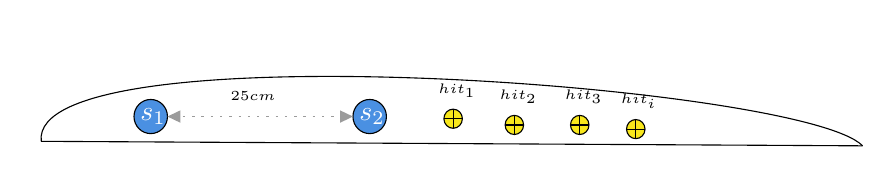
\begin{tikzpicture}[x=0.75pt,y=0.75pt,yscale=-1,xscale=1]
%uncomment if require: \path (0,300); %set diagram left start at 0, and has height of 300

%Curve Lines [id:da37291442444066547] 
\draw    (57,87) .. controls (50.74,32.51) and (424.54,59.84) .. (452.74,89.17) ;
%Straight Lines [id:da5213498635173044] 
\draw    (57,87) -- (452.74,89.17) ;
%Shape: Ellipse [id:dp5451517635936938] 
\draw  [color={rgb, 255:red, 0; green, 0; blue, 0 }  ,draw opacity=1 ][fill={rgb, 255:red, 74; green, 144; blue, 226 }  ,fill opacity=1 ] (101.7,75.06) .. controls (101.7,70.51) and (105.31,66.83) .. (109.76,66.83) .. controls (114.21,66.83) and (117.82,70.51) .. (117.82,75.06) .. controls (117.82,79.6) and (114.21,83.28) .. (109.76,83.28) .. controls (105.31,83.28) and (101.7,79.6) .. (101.7,75.06) -- cycle ;
\draw  [fill={rgb, 255:red, 248; green, 231; blue, 28 }  ,fill opacity=1 ] (251,76.11) .. controls (251,73.56) and (253,71.5) .. (255.46,71.5) .. controls (257.92,71.5) and (259.91,73.56) .. (259.91,76.11) .. controls (259.91,78.65) and (257.92,80.72) .. (255.46,80.72) .. controls (253,80.72) and (251,78.65) .. (251,76.11) -- cycle ; \draw   (251,76.11) -- (259.91,76.11) ; \draw   (255.46,71.5) -- (255.46,80.72) ;
%Shape: Ellipse [id:dp5239731363628557] 
\draw  [color={rgb, 255:red, 0; green, 0; blue, 0 }  ,draw opacity=1 ][fill={rgb, 255:red, 74; green, 144; blue, 226 }  ,fill opacity=1 ] (207.2,75.06) .. controls (207.2,70.51) and (210.81,66.83) .. (215.26,66.83) .. controls (219.71,66.83) and (223.32,70.51) .. (223.32,75.06) .. controls (223.32,79.6) and (219.71,83.28) .. (215.26,83.28) .. controls (210.81,83.28) and (207.2,79.6) .. (207.2,75.06) -- cycle ;
%Straight Lines [id:da7318958622897511] 
\draw [color={rgb, 255:red, 155; green, 155; blue, 155 }  ,draw opacity=1 ] [dash pattern={on 0.84pt off 2.51pt}]  (120.82,75.06) -- (204.2,75.06) ;
\draw [shift={(207.2,75.06)}, rotate = 180] [fill={rgb, 255:red, 155; green, 155; blue, 155 }  ,fill opacity=1 ][line width=0.08]  [draw opacity=0] (6.25,-3) -- (0,0) -- (6.25,3) -- cycle    ;
\draw [shift={(117.82,75.06)}, rotate = 0] [fill={rgb, 255:red, 155; green, 155; blue, 155 }  ,fill opacity=1 ][line width=0.08]  [draw opacity=0] (6.25,-3) -- (0,0) -- (6.25,3) -- cycle    ;
\draw  [fill={rgb, 255:red, 248; green, 231; blue, 28 }  ,fill opacity=1 ] (280.5,79.11) .. controls (280.5,76.56) and (282.5,74.5) .. (284.96,74.5) .. controls (287.42,74.5) and (289.41,76.56) .. (289.41,79.11) .. controls (289.41,81.65) and (287.42,83.72) .. (284.96,83.72) .. controls (282.5,83.72) and (280.5,81.65) .. (280.5,79.11) -- cycle ; \draw   (280.5,79.11) -- (289.41,79.11) ; \draw   (284.96,74.5) -- (284.96,83.72) ;
\draw  [fill={rgb, 255:red, 248; green, 231; blue, 28 }  ,fill opacity=1 ] (312,79.11) .. controls (312,76.56) and (314,74.5) .. (316.46,74.5) .. controls (318.92,74.5) and (320.91,76.56) .. (320.91,79.11) .. controls (320.91,81.65) and (318.92,83.72) .. (316.46,83.72) .. controls (314,83.72) and (312,81.65) .. (312,79.11) -- cycle ; \draw   (312,79.11) -- (320.91,79.11) ; \draw   (316.46,74.5) -- (316.46,83.72) ;
\draw  [fill={rgb, 255:red, 248; green, 231; blue, 28 }  ,fill opacity=1 ] (339,81.11) .. controls (339,78.56) and (341,76.5) .. (343.46,76.5) .. controls (345.92,76.5) and (347.91,78.56) .. (347.91,81.11) .. controls (347.91,83.65) and (345.92,85.72) .. (343.46,85.72) .. controls (341,85.72) and (339,83.65) .. (339,81.11) -- cycle ; \draw   (339,81.11) -- (347.91,81.11) ; \draw   (343.46,76.5) -- (343.46,85.72) ;

% Text Node
\draw (103.56,69.94) node [anchor=north west][inner sep=0.75pt]  [color={rgb, 255:red, 255; green, 255; blue, 255 }  ,opacity=1 ] [align=left] {$\displaystyle s_{1}$};
% Text Node
\draw (209.06,69.94) node [anchor=north west][inner sep=0.75pt]  [color={rgb, 255:red, 255; green, 255; blue, 255 }  ,opacity=1 ] [align=left] {$\displaystyle s_{2}$};
% Text Node
\draw (147,62) node [anchor=north west][inner sep=0.75pt]  [font=\tiny] [align=left] {$\displaystyle 25cm\ $};
% Text Node
\draw (247.06,57.94) node [anchor=north west][inner sep=0.75pt]  [font=\tiny,color={rgb, 255:red, 0; green, 0; blue, 0 }  ,opacity=1 ] [align=left] {$\displaystyle hit_{1}$};
% Text Node
\draw (276.56,60.94) node [anchor=north west][inner sep=0.75pt]  [font=\tiny,color={rgb, 255:red, 0; green, 0; blue, 0 }  ,opacity=1 ] [align=left] {$\displaystyle hit_{2}$};
% Text Node
\draw (308.06,60.94) node [anchor=north west][inner sep=0.75pt]  [font=\tiny,color={rgb, 255:red, 0; green, 0; blue, 0 }  ,opacity=1 ] [align=left] {$\displaystyle hit_{3}$};
% Text Node
\draw (335.06,62.94) node [anchor=north west][inner sep=0.75pt]  [font=\tiny,color={rgb, 255:red, 0; green, 0; blue, 0 }  ,opacity=1 ] [align=left] {$\displaystyle hit_{i}$};


\end{tikzpicture}}
        \caption{Experiment Visualization }
        \label{fig:label}
    \end{figure}

To make it easy for me, i have implemented a Signal class in python with
different modes one for attenuation, velocity calculation, and
localization. Each one has its own feature, but the common attribute
among them is the arrival time. It is calculated with AIC method
(discussed in next part). We know that:\\
{\[velocity = \frac{distance}{time}\]}By which we can compute the mean
velocity of different hits through the following equation:\\
{\[\overline{v} = \frac{1}{n}\sum\limits_{i = 1}^{n}\frac{d}{|t_{i,1} - t_{i,2}|}\]}Where,

\begin{itemize}

\item
  {\(d\)} is the distance between the two sensors that equals
  {\(25cm\)}.
\item
  {\(n\)} is the number of hits.
\item
  {\(t_{i,1}\)} is the arrival time of the signal to sensor {\(1\)} from
  hit {\(i\)}
\item
  {\(t_{i,2}\)} is the arrival time of the signal to sensor {\(2\)} from
  hit {\(i\)}
\end{itemize}

    \begin{figure}[htbp]
        \centering
        \scalebox{0.5}{%% Creator: Matplotlib, PGF backend
%%
%% To include the figure in your LaTeX document, write
%%   \input{<filename>.pgf}
%%
%% Make sure the required packages are loaded in your preamble
%%   \usepackage{pgf}
%%
%% Also ensure that all the required font packages are loaded; for instance,
%% the lmodern package is sometimes necessary when using math font.
%%   \usepackage{lmodern}
%%
%% Figures using additional raster images can only be included by \input if
%% they are in the same directory as the main LaTeX file. For loading figures
%% from other directories you can use the `import` package
%%   \usepackage{import}
%%
%% and then include the figures with
%%   \import{<path to file>}{<filename>.pgf}
%%
%% Matplotlib used the following preamble
%%
\begingroup%
\makeatletter%
\begin{pgfpicture}%
\pgfpathrectangle{\pgfpointorigin}{\pgfqpoint{9.968212in}{6.323786in}}%
\pgfusepath{use as bounding box, clip}%
\begin{pgfscope}%
\pgfsetbuttcap%
\pgfsetmiterjoin%
\definecolor{currentfill}{rgb}{1.000000,1.000000,1.000000}%
\pgfsetfillcolor{currentfill}%
\pgfsetlinewidth{0.000000pt}%
\definecolor{currentstroke}{rgb}{1.000000,1.000000,1.000000}%
\pgfsetstrokecolor{currentstroke}%
\pgfsetdash{}{0pt}%
\pgfpathmoveto{\pgfqpoint{0.000000in}{0.000000in}}%
\pgfpathlineto{\pgfqpoint{9.968212in}{0.000000in}}%
\pgfpathlineto{\pgfqpoint{9.968212in}{6.323786in}}%
\pgfpathlineto{\pgfqpoint{0.000000in}{6.323786in}}%
\pgfpathlineto{\pgfqpoint{0.000000in}{0.000000in}}%
\pgfpathclose%
\pgfusepath{fill}%
\end{pgfscope}%
\begin{pgfscope}%
\pgfsetbuttcap%
\pgfsetmiterjoin%
\definecolor{currentfill}{rgb}{1.000000,1.000000,1.000000}%
\pgfsetfillcolor{currentfill}%
\pgfsetlinewidth{0.000000pt}%
\definecolor{currentstroke}{rgb}{0.000000,0.000000,0.000000}%
\pgfsetstrokecolor{currentstroke}%
\pgfsetstrokeopacity{0.000000}%
\pgfsetdash{}{0pt}%
\pgfpathmoveto{\pgfqpoint{0.908293in}{0.718286in}}%
\pgfpathlineto{\pgfqpoint{8.968293in}{0.718286in}}%
\pgfpathlineto{\pgfqpoint{8.968293in}{6.223786in}}%
\pgfpathlineto{\pgfqpoint{0.908293in}{6.223786in}}%
\pgfpathlineto{\pgfqpoint{0.908293in}{0.718286in}}%
\pgfpathclose%
\pgfusepath{fill}%
\end{pgfscope}%
\begin{pgfscope}%
\pgfpathrectangle{\pgfqpoint{0.908293in}{0.718286in}}{\pgfqpoint{8.060000in}{5.505500in}}%
\pgfusepath{clip}%
\pgfsetrectcap%
\pgfsetroundjoin%
\pgfsetlinewidth{1.304875pt}%
\definecolor{currentstroke}{rgb}{0.690196,0.690196,0.690196}%
\pgfsetstrokecolor{currentstroke}%
\pgfsetdash{}{0pt}%
\pgfpathmoveto{\pgfqpoint{1.203101in}{0.718286in}}%
\pgfpathlineto{\pgfqpoint{1.203101in}{6.223786in}}%
\pgfusepath{stroke}%
\end{pgfscope}%
\begin{pgfscope}%
\pgfsetbuttcap%
\pgfsetroundjoin%
\definecolor{currentfill}{rgb}{0.000000,0.000000,0.000000}%
\pgfsetfillcolor{currentfill}%
\pgfsetlinewidth{1.304875pt}%
\definecolor{currentstroke}{rgb}{0.000000,0.000000,0.000000}%
\pgfsetstrokecolor{currentstroke}%
\pgfsetdash{}{0pt}%
\pgfsys@defobject{currentmarker}{\pgfqpoint{0.000000in}{-0.048611in}}{\pgfqpoint{0.000000in}{0.000000in}}{%
\pgfpathmoveto{\pgfqpoint{0.000000in}{0.000000in}}%
\pgfpathlineto{\pgfqpoint{0.000000in}{-0.048611in}}%
\pgfusepath{stroke,fill}%
}%
\begin{pgfscope}%
\pgfsys@transformshift{1.203101in}{0.718286in}%
\pgfsys@useobject{currentmarker}{}%
\end{pgfscope}%
\end{pgfscope}%
\begin{pgfscope}%
\definecolor{textcolor}{rgb}{0.000000,0.000000,0.000000}%
\pgfsetstrokecolor{textcolor}%
\pgfsetfillcolor{textcolor}%
\pgftext[x=1.203101in,y=0.543286in,,top]{\color{textcolor}\rmfamily\fontsize{13.000000}{15.600000}\selectfont \(\displaystyle {0.00065}\)}%
\end{pgfscope}%
\begin{pgfscope}%
\pgfpathrectangle{\pgfqpoint{0.908293in}{0.718286in}}{\pgfqpoint{8.060000in}{5.505500in}}%
\pgfusepath{clip}%
\pgfsetrectcap%
\pgfsetroundjoin%
\pgfsetlinewidth{1.304875pt}%
\definecolor{currentstroke}{rgb}{0.690196,0.690196,0.690196}%
\pgfsetstrokecolor{currentstroke}%
\pgfsetdash{}{0pt}%
\pgfpathmoveto{\pgfqpoint{2.991986in}{0.718286in}}%
\pgfpathlineto{\pgfqpoint{2.991986in}{6.223786in}}%
\pgfusepath{stroke}%
\end{pgfscope}%
\begin{pgfscope}%
\pgfsetbuttcap%
\pgfsetroundjoin%
\definecolor{currentfill}{rgb}{0.000000,0.000000,0.000000}%
\pgfsetfillcolor{currentfill}%
\pgfsetlinewidth{1.304875pt}%
\definecolor{currentstroke}{rgb}{0.000000,0.000000,0.000000}%
\pgfsetstrokecolor{currentstroke}%
\pgfsetdash{}{0pt}%
\pgfsys@defobject{currentmarker}{\pgfqpoint{0.000000in}{-0.048611in}}{\pgfqpoint{0.000000in}{0.000000in}}{%
\pgfpathmoveto{\pgfqpoint{0.000000in}{0.000000in}}%
\pgfpathlineto{\pgfqpoint{0.000000in}{-0.048611in}}%
\pgfusepath{stroke,fill}%
}%
\begin{pgfscope}%
\pgfsys@transformshift{2.991986in}{0.718286in}%
\pgfsys@useobject{currentmarker}{}%
\end{pgfscope}%
\end{pgfscope}%
\begin{pgfscope}%
\definecolor{textcolor}{rgb}{0.000000,0.000000,0.000000}%
\pgfsetstrokecolor{textcolor}%
\pgfsetfillcolor{textcolor}%
\pgftext[x=2.991986in,y=0.543286in,,top]{\color{textcolor}\rmfamily\fontsize{13.000000}{15.600000}\selectfont \(\displaystyle {0.00070}\)}%
\end{pgfscope}%
\begin{pgfscope}%
\pgfpathrectangle{\pgfqpoint{0.908293in}{0.718286in}}{\pgfqpoint{8.060000in}{5.505500in}}%
\pgfusepath{clip}%
\pgfsetrectcap%
\pgfsetroundjoin%
\pgfsetlinewidth{1.304875pt}%
\definecolor{currentstroke}{rgb}{0.690196,0.690196,0.690196}%
\pgfsetstrokecolor{currentstroke}%
\pgfsetdash{}{0pt}%
\pgfpathmoveto{\pgfqpoint{4.780871in}{0.718286in}}%
\pgfpathlineto{\pgfqpoint{4.780871in}{6.223786in}}%
\pgfusepath{stroke}%
\end{pgfscope}%
\begin{pgfscope}%
\pgfsetbuttcap%
\pgfsetroundjoin%
\definecolor{currentfill}{rgb}{0.000000,0.000000,0.000000}%
\pgfsetfillcolor{currentfill}%
\pgfsetlinewidth{1.304875pt}%
\definecolor{currentstroke}{rgb}{0.000000,0.000000,0.000000}%
\pgfsetstrokecolor{currentstroke}%
\pgfsetdash{}{0pt}%
\pgfsys@defobject{currentmarker}{\pgfqpoint{0.000000in}{-0.048611in}}{\pgfqpoint{0.000000in}{0.000000in}}{%
\pgfpathmoveto{\pgfqpoint{0.000000in}{0.000000in}}%
\pgfpathlineto{\pgfqpoint{0.000000in}{-0.048611in}}%
\pgfusepath{stroke,fill}%
}%
\begin{pgfscope}%
\pgfsys@transformshift{4.780871in}{0.718286in}%
\pgfsys@useobject{currentmarker}{}%
\end{pgfscope}%
\end{pgfscope}%
\begin{pgfscope}%
\definecolor{textcolor}{rgb}{0.000000,0.000000,0.000000}%
\pgfsetstrokecolor{textcolor}%
\pgfsetfillcolor{textcolor}%
\pgftext[x=4.780871in,y=0.543286in,,top]{\color{textcolor}\rmfamily\fontsize{13.000000}{15.600000}\selectfont \(\displaystyle {0.00075}\)}%
\end{pgfscope}%
\begin{pgfscope}%
\pgfpathrectangle{\pgfqpoint{0.908293in}{0.718286in}}{\pgfqpoint{8.060000in}{5.505500in}}%
\pgfusepath{clip}%
\pgfsetrectcap%
\pgfsetroundjoin%
\pgfsetlinewidth{1.304875pt}%
\definecolor{currentstroke}{rgb}{0.690196,0.690196,0.690196}%
\pgfsetstrokecolor{currentstroke}%
\pgfsetdash{}{0pt}%
\pgfpathmoveto{\pgfqpoint{6.569756in}{0.718286in}}%
\pgfpathlineto{\pgfqpoint{6.569756in}{6.223786in}}%
\pgfusepath{stroke}%
\end{pgfscope}%
\begin{pgfscope}%
\pgfsetbuttcap%
\pgfsetroundjoin%
\definecolor{currentfill}{rgb}{0.000000,0.000000,0.000000}%
\pgfsetfillcolor{currentfill}%
\pgfsetlinewidth{1.304875pt}%
\definecolor{currentstroke}{rgb}{0.000000,0.000000,0.000000}%
\pgfsetstrokecolor{currentstroke}%
\pgfsetdash{}{0pt}%
\pgfsys@defobject{currentmarker}{\pgfqpoint{0.000000in}{-0.048611in}}{\pgfqpoint{0.000000in}{0.000000in}}{%
\pgfpathmoveto{\pgfqpoint{0.000000in}{0.000000in}}%
\pgfpathlineto{\pgfqpoint{0.000000in}{-0.048611in}}%
\pgfusepath{stroke,fill}%
}%
\begin{pgfscope}%
\pgfsys@transformshift{6.569756in}{0.718286in}%
\pgfsys@useobject{currentmarker}{}%
\end{pgfscope}%
\end{pgfscope}%
\begin{pgfscope}%
\definecolor{textcolor}{rgb}{0.000000,0.000000,0.000000}%
\pgfsetstrokecolor{textcolor}%
\pgfsetfillcolor{textcolor}%
\pgftext[x=6.569756in,y=0.543286in,,top]{\color{textcolor}\rmfamily\fontsize{13.000000}{15.600000}\selectfont \(\displaystyle {0.00080}\)}%
\end{pgfscope}%
\begin{pgfscope}%
\pgfpathrectangle{\pgfqpoint{0.908293in}{0.718286in}}{\pgfqpoint{8.060000in}{5.505500in}}%
\pgfusepath{clip}%
\pgfsetrectcap%
\pgfsetroundjoin%
\pgfsetlinewidth{1.304875pt}%
\definecolor{currentstroke}{rgb}{0.690196,0.690196,0.690196}%
\pgfsetstrokecolor{currentstroke}%
\pgfsetdash{}{0pt}%
\pgfpathmoveto{\pgfqpoint{8.358641in}{0.718286in}}%
\pgfpathlineto{\pgfqpoint{8.358641in}{6.223786in}}%
\pgfusepath{stroke}%
\end{pgfscope}%
\begin{pgfscope}%
\pgfsetbuttcap%
\pgfsetroundjoin%
\definecolor{currentfill}{rgb}{0.000000,0.000000,0.000000}%
\pgfsetfillcolor{currentfill}%
\pgfsetlinewidth{1.304875pt}%
\definecolor{currentstroke}{rgb}{0.000000,0.000000,0.000000}%
\pgfsetstrokecolor{currentstroke}%
\pgfsetdash{}{0pt}%
\pgfsys@defobject{currentmarker}{\pgfqpoint{0.000000in}{-0.048611in}}{\pgfqpoint{0.000000in}{0.000000in}}{%
\pgfpathmoveto{\pgfqpoint{0.000000in}{0.000000in}}%
\pgfpathlineto{\pgfqpoint{0.000000in}{-0.048611in}}%
\pgfusepath{stroke,fill}%
}%
\begin{pgfscope}%
\pgfsys@transformshift{8.358641in}{0.718286in}%
\pgfsys@useobject{currentmarker}{}%
\end{pgfscope}%
\end{pgfscope}%
\begin{pgfscope}%
\definecolor{textcolor}{rgb}{0.000000,0.000000,0.000000}%
\pgfsetstrokecolor{textcolor}%
\pgfsetfillcolor{textcolor}%
\pgftext[x=8.358641in,y=0.543286in,,top]{\color{textcolor}\rmfamily\fontsize{13.000000}{15.600000}\selectfont \(\displaystyle {0.00085}\)}%
\end{pgfscope}%
\begin{pgfscope}%
\definecolor{textcolor}{rgb}{0.000000,0.000000,0.000000}%
\pgfsetstrokecolor{textcolor}%
\pgfsetfillcolor{textcolor}%
\pgftext[x=4.938293in,y=0.339583in,,top]{\color{textcolor}\rmfamily\fontsize{17.000000}{20.400000}\selectfont time \(\displaystyle [s]\)}%
\end{pgfscope}%
\begin{pgfscope}%
\definecolor{textcolor}{rgb}{0.000000,0.000000,0.000000}%
\pgfsetstrokecolor{textcolor}%
\pgfsetfillcolor{textcolor}%
\pgftext[x=8.968293in,y=0.353472in,right,top]{\color{textcolor}\rmfamily\fontsize{13.000000}{15.600000}\selectfont \(\displaystyle {+1.65405 \times 10^{3}}\)}%
\end{pgfscope}%
\begin{pgfscope}%
\pgfpathrectangle{\pgfqpoint{0.908293in}{0.718286in}}{\pgfqpoint{8.060000in}{5.505500in}}%
\pgfusepath{clip}%
\pgfsetrectcap%
\pgfsetroundjoin%
\pgfsetlinewidth{1.304875pt}%
\definecolor{currentstroke}{rgb}{0.690196,0.690196,0.690196}%
\pgfsetstrokecolor{currentstroke}%
\pgfsetdash{}{0pt}%
\pgfpathmoveto{\pgfqpoint{0.908293in}{0.788861in}}%
\pgfpathlineto{\pgfqpoint{8.968293in}{0.788861in}}%
\pgfusepath{stroke}%
\end{pgfscope}%
\begin{pgfscope}%
\pgfsetbuttcap%
\pgfsetroundjoin%
\definecolor{currentfill}{rgb}{0.000000,0.000000,0.000000}%
\pgfsetfillcolor{currentfill}%
\pgfsetlinewidth{1.304875pt}%
\definecolor{currentstroke}{rgb}{0.000000,0.000000,0.000000}%
\pgfsetstrokecolor{currentstroke}%
\pgfsetdash{}{0pt}%
\pgfsys@defobject{currentmarker}{\pgfqpoint{-0.048611in}{0.000000in}}{\pgfqpoint{-0.000000in}{0.000000in}}{%
\pgfpathmoveto{\pgfqpoint{-0.000000in}{0.000000in}}%
\pgfpathlineto{\pgfqpoint{-0.048611in}{0.000000in}}%
\pgfusepath{stroke,fill}%
}%
\begin{pgfscope}%
\pgfsys@transformshift{0.908293in}{0.788861in}%
\pgfsys@useobject{currentmarker}{}%
\end{pgfscope}%
\end{pgfscope}%
\begin{pgfscope}%
\definecolor{textcolor}{rgb}{0.000000,0.000000,0.000000}%
\pgfsetstrokecolor{textcolor}%
\pgfsetfillcolor{textcolor}%
\pgftext[x=0.395138in, y=0.730991in, left, base]{\color{textcolor}\rmfamily\fontsize{13.000000}{15.600000}\selectfont \(\displaystyle {\ensuremath{-}0.3}\)}%
\end{pgfscope}%
\begin{pgfscope}%
\pgfpathrectangle{\pgfqpoint{0.908293in}{0.718286in}}{\pgfqpoint{8.060000in}{5.505500in}}%
\pgfusepath{clip}%
\pgfsetrectcap%
\pgfsetroundjoin%
\pgfsetlinewidth{1.304875pt}%
\definecolor{currentstroke}{rgb}{0.690196,0.690196,0.690196}%
\pgfsetstrokecolor{currentstroke}%
\pgfsetdash{}{0pt}%
\pgfpathmoveto{\pgfqpoint{0.908293in}{1.435564in}}%
\pgfpathlineto{\pgfqpoint{8.968293in}{1.435564in}}%
\pgfusepath{stroke}%
\end{pgfscope}%
\begin{pgfscope}%
\pgfsetbuttcap%
\pgfsetroundjoin%
\definecolor{currentfill}{rgb}{0.000000,0.000000,0.000000}%
\pgfsetfillcolor{currentfill}%
\pgfsetlinewidth{1.304875pt}%
\definecolor{currentstroke}{rgb}{0.000000,0.000000,0.000000}%
\pgfsetstrokecolor{currentstroke}%
\pgfsetdash{}{0pt}%
\pgfsys@defobject{currentmarker}{\pgfqpoint{-0.048611in}{0.000000in}}{\pgfqpoint{-0.000000in}{0.000000in}}{%
\pgfpathmoveto{\pgfqpoint{-0.000000in}{0.000000in}}%
\pgfpathlineto{\pgfqpoint{-0.048611in}{0.000000in}}%
\pgfusepath{stroke,fill}%
}%
\begin{pgfscope}%
\pgfsys@transformshift{0.908293in}{1.435564in}%
\pgfsys@useobject{currentmarker}{}%
\end{pgfscope}%
\end{pgfscope}%
\begin{pgfscope}%
\definecolor{textcolor}{rgb}{0.000000,0.000000,0.000000}%
\pgfsetstrokecolor{textcolor}%
\pgfsetfillcolor{textcolor}%
\pgftext[x=0.395138in, y=1.377694in, left, base]{\color{textcolor}\rmfamily\fontsize{13.000000}{15.600000}\selectfont \(\displaystyle {\ensuremath{-}0.2}\)}%
\end{pgfscope}%
\begin{pgfscope}%
\pgfpathrectangle{\pgfqpoint{0.908293in}{0.718286in}}{\pgfqpoint{8.060000in}{5.505500in}}%
\pgfusepath{clip}%
\pgfsetrectcap%
\pgfsetroundjoin%
\pgfsetlinewidth{1.304875pt}%
\definecolor{currentstroke}{rgb}{0.690196,0.690196,0.690196}%
\pgfsetstrokecolor{currentstroke}%
\pgfsetdash{}{0pt}%
\pgfpathmoveto{\pgfqpoint{0.908293in}{2.082267in}}%
\pgfpathlineto{\pgfqpoint{8.968293in}{2.082267in}}%
\pgfusepath{stroke}%
\end{pgfscope}%
\begin{pgfscope}%
\pgfsetbuttcap%
\pgfsetroundjoin%
\definecolor{currentfill}{rgb}{0.000000,0.000000,0.000000}%
\pgfsetfillcolor{currentfill}%
\pgfsetlinewidth{1.304875pt}%
\definecolor{currentstroke}{rgb}{0.000000,0.000000,0.000000}%
\pgfsetstrokecolor{currentstroke}%
\pgfsetdash{}{0pt}%
\pgfsys@defobject{currentmarker}{\pgfqpoint{-0.048611in}{0.000000in}}{\pgfqpoint{-0.000000in}{0.000000in}}{%
\pgfpathmoveto{\pgfqpoint{-0.000000in}{0.000000in}}%
\pgfpathlineto{\pgfqpoint{-0.048611in}{0.000000in}}%
\pgfusepath{stroke,fill}%
}%
\begin{pgfscope}%
\pgfsys@transformshift{0.908293in}{2.082267in}%
\pgfsys@useobject{currentmarker}{}%
\end{pgfscope}%
\end{pgfscope}%
\begin{pgfscope}%
\definecolor{textcolor}{rgb}{0.000000,0.000000,0.000000}%
\pgfsetstrokecolor{textcolor}%
\pgfsetfillcolor{textcolor}%
\pgftext[x=0.395138in, y=2.024397in, left, base]{\color{textcolor}\rmfamily\fontsize{13.000000}{15.600000}\selectfont \(\displaystyle {\ensuremath{-}0.1}\)}%
\end{pgfscope}%
\begin{pgfscope}%
\pgfpathrectangle{\pgfqpoint{0.908293in}{0.718286in}}{\pgfqpoint{8.060000in}{5.505500in}}%
\pgfusepath{clip}%
\pgfsetrectcap%
\pgfsetroundjoin%
\pgfsetlinewidth{1.304875pt}%
\definecolor{currentstroke}{rgb}{0.690196,0.690196,0.690196}%
\pgfsetstrokecolor{currentstroke}%
\pgfsetdash{}{0pt}%
\pgfpathmoveto{\pgfqpoint{0.908293in}{2.728970in}}%
\pgfpathlineto{\pgfqpoint{8.968293in}{2.728970in}}%
\pgfusepath{stroke}%
\end{pgfscope}%
\begin{pgfscope}%
\pgfsetbuttcap%
\pgfsetroundjoin%
\definecolor{currentfill}{rgb}{0.000000,0.000000,0.000000}%
\pgfsetfillcolor{currentfill}%
\pgfsetlinewidth{1.304875pt}%
\definecolor{currentstroke}{rgb}{0.000000,0.000000,0.000000}%
\pgfsetstrokecolor{currentstroke}%
\pgfsetdash{}{0pt}%
\pgfsys@defobject{currentmarker}{\pgfqpoint{-0.048611in}{0.000000in}}{\pgfqpoint{-0.000000in}{0.000000in}}{%
\pgfpathmoveto{\pgfqpoint{-0.000000in}{0.000000in}}%
\pgfpathlineto{\pgfqpoint{-0.048611in}{0.000000in}}%
\pgfusepath{stroke,fill}%
}%
\begin{pgfscope}%
\pgfsys@transformshift{0.908293in}{2.728970in}%
\pgfsys@useobject{currentmarker}{}%
\end{pgfscope}%
\end{pgfscope}%
\begin{pgfscope}%
\definecolor{textcolor}{rgb}{0.000000,0.000000,0.000000}%
\pgfsetstrokecolor{textcolor}%
\pgfsetfillcolor{textcolor}%
\pgftext[x=0.524768in, y=2.671100in, left, base]{\color{textcolor}\rmfamily\fontsize{13.000000}{15.600000}\selectfont \(\displaystyle {0.0}\)}%
\end{pgfscope}%
\begin{pgfscope}%
\pgfpathrectangle{\pgfqpoint{0.908293in}{0.718286in}}{\pgfqpoint{8.060000in}{5.505500in}}%
\pgfusepath{clip}%
\pgfsetrectcap%
\pgfsetroundjoin%
\pgfsetlinewidth{1.304875pt}%
\definecolor{currentstroke}{rgb}{0.690196,0.690196,0.690196}%
\pgfsetstrokecolor{currentstroke}%
\pgfsetdash{}{0pt}%
\pgfpathmoveto{\pgfqpoint{0.908293in}{3.375673in}}%
\pgfpathlineto{\pgfqpoint{8.968293in}{3.375673in}}%
\pgfusepath{stroke}%
\end{pgfscope}%
\begin{pgfscope}%
\pgfsetbuttcap%
\pgfsetroundjoin%
\definecolor{currentfill}{rgb}{0.000000,0.000000,0.000000}%
\pgfsetfillcolor{currentfill}%
\pgfsetlinewidth{1.304875pt}%
\definecolor{currentstroke}{rgb}{0.000000,0.000000,0.000000}%
\pgfsetstrokecolor{currentstroke}%
\pgfsetdash{}{0pt}%
\pgfsys@defobject{currentmarker}{\pgfqpoint{-0.048611in}{0.000000in}}{\pgfqpoint{-0.000000in}{0.000000in}}{%
\pgfpathmoveto{\pgfqpoint{-0.000000in}{0.000000in}}%
\pgfpathlineto{\pgfqpoint{-0.048611in}{0.000000in}}%
\pgfusepath{stroke,fill}%
}%
\begin{pgfscope}%
\pgfsys@transformshift{0.908293in}{3.375673in}%
\pgfsys@useobject{currentmarker}{}%
\end{pgfscope}%
\end{pgfscope}%
\begin{pgfscope}%
\definecolor{textcolor}{rgb}{0.000000,0.000000,0.000000}%
\pgfsetstrokecolor{textcolor}%
\pgfsetfillcolor{textcolor}%
\pgftext[x=0.524768in, y=3.317802in, left, base]{\color{textcolor}\rmfamily\fontsize{13.000000}{15.600000}\selectfont \(\displaystyle {0.1}\)}%
\end{pgfscope}%
\begin{pgfscope}%
\pgfpathrectangle{\pgfqpoint{0.908293in}{0.718286in}}{\pgfqpoint{8.060000in}{5.505500in}}%
\pgfusepath{clip}%
\pgfsetrectcap%
\pgfsetroundjoin%
\pgfsetlinewidth{1.304875pt}%
\definecolor{currentstroke}{rgb}{0.690196,0.690196,0.690196}%
\pgfsetstrokecolor{currentstroke}%
\pgfsetdash{}{0pt}%
\pgfpathmoveto{\pgfqpoint{0.908293in}{4.022375in}}%
\pgfpathlineto{\pgfqpoint{8.968293in}{4.022375in}}%
\pgfusepath{stroke}%
\end{pgfscope}%
\begin{pgfscope}%
\pgfsetbuttcap%
\pgfsetroundjoin%
\definecolor{currentfill}{rgb}{0.000000,0.000000,0.000000}%
\pgfsetfillcolor{currentfill}%
\pgfsetlinewidth{1.304875pt}%
\definecolor{currentstroke}{rgb}{0.000000,0.000000,0.000000}%
\pgfsetstrokecolor{currentstroke}%
\pgfsetdash{}{0pt}%
\pgfsys@defobject{currentmarker}{\pgfqpoint{-0.048611in}{0.000000in}}{\pgfqpoint{-0.000000in}{0.000000in}}{%
\pgfpathmoveto{\pgfqpoint{-0.000000in}{0.000000in}}%
\pgfpathlineto{\pgfqpoint{-0.048611in}{0.000000in}}%
\pgfusepath{stroke,fill}%
}%
\begin{pgfscope}%
\pgfsys@transformshift{0.908293in}{4.022375in}%
\pgfsys@useobject{currentmarker}{}%
\end{pgfscope}%
\end{pgfscope}%
\begin{pgfscope}%
\definecolor{textcolor}{rgb}{0.000000,0.000000,0.000000}%
\pgfsetstrokecolor{textcolor}%
\pgfsetfillcolor{textcolor}%
\pgftext[x=0.524768in, y=3.964505in, left, base]{\color{textcolor}\rmfamily\fontsize{13.000000}{15.600000}\selectfont \(\displaystyle {0.2}\)}%
\end{pgfscope}%
\begin{pgfscope}%
\pgfpathrectangle{\pgfqpoint{0.908293in}{0.718286in}}{\pgfqpoint{8.060000in}{5.505500in}}%
\pgfusepath{clip}%
\pgfsetrectcap%
\pgfsetroundjoin%
\pgfsetlinewidth{1.304875pt}%
\definecolor{currentstroke}{rgb}{0.690196,0.690196,0.690196}%
\pgfsetstrokecolor{currentstroke}%
\pgfsetdash{}{0pt}%
\pgfpathmoveto{\pgfqpoint{0.908293in}{4.669078in}}%
\pgfpathlineto{\pgfqpoint{8.968293in}{4.669078in}}%
\pgfusepath{stroke}%
\end{pgfscope}%
\begin{pgfscope}%
\pgfsetbuttcap%
\pgfsetroundjoin%
\definecolor{currentfill}{rgb}{0.000000,0.000000,0.000000}%
\pgfsetfillcolor{currentfill}%
\pgfsetlinewidth{1.304875pt}%
\definecolor{currentstroke}{rgb}{0.000000,0.000000,0.000000}%
\pgfsetstrokecolor{currentstroke}%
\pgfsetdash{}{0pt}%
\pgfsys@defobject{currentmarker}{\pgfqpoint{-0.048611in}{0.000000in}}{\pgfqpoint{-0.000000in}{0.000000in}}{%
\pgfpathmoveto{\pgfqpoint{-0.000000in}{0.000000in}}%
\pgfpathlineto{\pgfqpoint{-0.048611in}{0.000000in}}%
\pgfusepath{stroke,fill}%
}%
\begin{pgfscope}%
\pgfsys@transformshift{0.908293in}{4.669078in}%
\pgfsys@useobject{currentmarker}{}%
\end{pgfscope}%
\end{pgfscope}%
\begin{pgfscope}%
\definecolor{textcolor}{rgb}{0.000000,0.000000,0.000000}%
\pgfsetstrokecolor{textcolor}%
\pgfsetfillcolor{textcolor}%
\pgftext[x=0.524768in, y=4.611208in, left, base]{\color{textcolor}\rmfamily\fontsize{13.000000}{15.600000}\selectfont \(\displaystyle {0.3}\)}%
\end{pgfscope}%
\begin{pgfscope}%
\pgfpathrectangle{\pgfqpoint{0.908293in}{0.718286in}}{\pgfqpoint{8.060000in}{5.505500in}}%
\pgfusepath{clip}%
\pgfsetrectcap%
\pgfsetroundjoin%
\pgfsetlinewidth{1.304875pt}%
\definecolor{currentstroke}{rgb}{0.690196,0.690196,0.690196}%
\pgfsetstrokecolor{currentstroke}%
\pgfsetdash{}{0pt}%
\pgfpathmoveto{\pgfqpoint{0.908293in}{5.315781in}}%
\pgfpathlineto{\pgfqpoint{8.968293in}{5.315781in}}%
\pgfusepath{stroke}%
\end{pgfscope}%
\begin{pgfscope}%
\pgfsetbuttcap%
\pgfsetroundjoin%
\definecolor{currentfill}{rgb}{0.000000,0.000000,0.000000}%
\pgfsetfillcolor{currentfill}%
\pgfsetlinewidth{1.304875pt}%
\definecolor{currentstroke}{rgb}{0.000000,0.000000,0.000000}%
\pgfsetstrokecolor{currentstroke}%
\pgfsetdash{}{0pt}%
\pgfsys@defobject{currentmarker}{\pgfqpoint{-0.048611in}{0.000000in}}{\pgfqpoint{-0.000000in}{0.000000in}}{%
\pgfpathmoveto{\pgfqpoint{-0.000000in}{0.000000in}}%
\pgfpathlineto{\pgfqpoint{-0.048611in}{0.000000in}}%
\pgfusepath{stroke,fill}%
}%
\begin{pgfscope}%
\pgfsys@transformshift{0.908293in}{5.315781in}%
\pgfsys@useobject{currentmarker}{}%
\end{pgfscope}%
\end{pgfscope}%
\begin{pgfscope}%
\definecolor{textcolor}{rgb}{0.000000,0.000000,0.000000}%
\pgfsetstrokecolor{textcolor}%
\pgfsetfillcolor{textcolor}%
\pgftext[x=0.524768in, y=5.257911in, left, base]{\color{textcolor}\rmfamily\fontsize{13.000000}{15.600000}\selectfont \(\displaystyle {0.4}\)}%
\end{pgfscope}%
\begin{pgfscope}%
\pgfpathrectangle{\pgfqpoint{0.908293in}{0.718286in}}{\pgfqpoint{8.060000in}{5.505500in}}%
\pgfusepath{clip}%
\pgfsetrectcap%
\pgfsetroundjoin%
\pgfsetlinewidth{1.304875pt}%
\definecolor{currentstroke}{rgb}{0.690196,0.690196,0.690196}%
\pgfsetstrokecolor{currentstroke}%
\pgfsetdash{}{0pt}%
\pgfpathmoveto{\pgfqpoint{0.908293in}{5.962484in}}%
\pgfpathlineto{\pgfqpoint{8.968293in}{5.962484in}}%
\pgfusepath{stroke}%
\end{pgfscope}%
\begin{pgfscope}%
\pgfsetbuttcap%
\pgfsetroundjoin%
\definecolor{currentfill}{rgb}{0.000000,0.000000,0.000000}%
\pgfsetfillcolor{currentfill}%
\pgfsetlinewidth{1.304875pt}%
\definecolor{currentstroke}{rgb}{0.000000,0.000000,0.000000}%
\pgfsetstrokecolor{currentstroke}%
\pgfsetdash{}{0pt}%
\pgfsys@defobject{currentmarker}{\pgfqpoint{-0.048611in}{0.000000in}}{\pgfqpoint{-0.000000in}{0.000000in}}{%
\pgfpathmoveto{\pgfqpoint{-0.000000in}{0.000000in}}%
\pgfpathlineto{\pgfqpoint{-0.048611in}{0.000000in}}%
\pgfusepath{stroke,fill}%
}%
\begin{pgfscope}%
\pgfsys@transformshift{0.908293in}{5.962484in}%
\pgfsys@useobject{currentmarker}{}%
\end{pgfscope}%
\end{pgfscope}%
\begin{pgfscope}%
\definecolor{textcolor}{rgb}{0.000000,0.000000,0.000000}%
\pgfsetstrokecolor{textcolor}%
\pgfsetfillcolor{textcolor}%
\pgftext[x=0.524768in, y=5.904614in, left, base]{\color{textcolor}\rmfamily\fontsize{13.000000}{15.600000}\selectfont \(\displaystyle {0.5}\)}%
\end{pgfscope}%
\begin{pgfscope}%
\definecolor{textcolor}{rgb}{0.000000,0.000000,0.000000}%
\pgfsetstrokecolor{textcolor}%
\pgfsetfillcolor{textcolor}%
\pgftext[x=0.339583in,y=3.471036in,,bottom,rotate=90.000000]{\color{textcolor}\rmfamily\fontsize{17.000000}{20.400000}\selectfont Amplitude[V]}%
\end{pgfscope}%
\begin{pgfscope}%
\pgfpathrectangle{\pgfqpoint{0.908293in}{0.718286in}}{\pgfqpoint{8.060000in}{5.505500in}}%
\pgfusepath{clip}%
\pgfsetrectcap%
\pgfsetroundjoin%
\pgfsetlinewidth{1.003750pt}%
\definecolor{currentstroke}{rgb}{0.000000,0.000000,1.000000}%
\pgfsetstrokecolor{currentstroke}%
\pgfsetdash{}{0pt}%
\pgfpathmoveto{\pgfqpoint{1.274656in}{2.717128in}}%
\pgfpathlineto{\pgfqpoint{1.281819in}{2.717128in}}%
\pgfpathlineto{\pgfqpoint{1.288981in}{2.715155in}}%
\pgfpathlineto{\pgfqpoint{1.296144in}{2.715155in}}%
\pgfpathlineto{\pgfqpoint{1.303306in}{2.713181in}}%
\pgfpathlineto{\pgfqpoint{1.317631in}{2.713181in}}%
\pgfpathlineto{\pgfqpoint{1.324794in}{2.715155in}}%
\pgfpathlineto{\pgfqpoint{1.331956in}{2.715155in}}%
\pgfpathlineto{\pgfqpoint{1.339119in}{2.717128in}}%
\pgfpathlineto{\pgfqpoint{1.346281in}{2.717128in}}%
\pgfpathlineto{\pgfqpoint{1.374932in}{2.725023in}}%
\pgfpathlineto{\pgfqpoint{1.382094in}{2.725023in}}%
\pgfpathlineto{\pgfqpoint{1.396419in}{2.728970in}}%
\pgfpathlineto{\pgfqpoint{1.403582in}{2.728970in}}%
\pgfpathlineto{\pgfqpoint{1.410744in}{2.730943in}}%
\pgfpathlineto{\pgfqpoint{1.417907in}{2.730943in}}%
\pgfpathlineto{\pgfqpoint{1.425069in}{2.732917in}}%
\pgfpathlineto{\pgfqpoint{1.475207in}{2.732917in}}%
\pgfpathlineto{\pgfqpoint{1.482370in}{2.730943in}}%
\pgfpathlineto{\pgfqpoint{1.496695in}{2.730943in}}%
\pgfpathlineto{\pgfqpoint{1.503857in}{2.728970in}}%
\pgfpathlineto{\pgfqpoint{1.568320in}{2.728970in}}%
\pgfpathlineto{\pgfqpoint{1.575483in}{2.730943in}}%
\pgfpathlineto{\pgfqpoint{1.625620in}{2.730943in}}%
\pgfpathlineto{\pgfqpoint{1.632783in}{2.732917in}}%
\pgfpathlineto{\pgfqpoint{1.668596in}{2.732917in}}%
\pgfpathlineto{\pgfqpoint{1.675758in}{2.734891in}}%
\pgfpathlineto{\pgfqpoint{1.697246in}{2.734891in}}%
\pgfpathlineto{\pgfqpoint{1.704408in}{2.732917in}}%
\pgfpathlineto{\pgfqpoint{1.725896in}{2.732917in}}%
\pgfpathlineto{\pgfqpoint{1.733058in}{2.730943in}}%
\pgfpathlineto{\pgfqpoint{1.768871in}{2.730943in}}%
\pgfpathlineto{\pgfqpoint{1.776034in}{2.732917in}}%
\pgfpathlineto{\pgfqpoint{1.783196in}{2.732917in}}%
\pgfpathlineto{\pgfqpoint{1.790359in}{2.734891in}}%
\pgfpathlineto{\pgfqpoint{1.797521in}{2.734891in}}%
\pgfpathlineto{\pgfqpoint{1.819009in}{2.740811in}}%
\pgfpathlineto{\pgfqpoint{1.826171in}{2.740811in}}%
\pgfpathlineto{\pgfqpoint{1.833334in}{2.742785in}}%
\pgfpathlineto{\pgfqpoint{1.861984in}{2.742785in}}%
\pgfpathlineto{\pgfqpoint{1.876309in}{2.738838in}}%
\pgfpathlineto{\pgfqpoint{1.883472in}{2.734891in}}%
\pgfpathlineto{\pgfqpoint{1.897797in}{2.723049in}}%
\pgfpathlineto{\pgfqpoint{1.912122in}{2.703313in}}%
\pgfpathlineto{\pgfqpoint{1.955097in}{2.620423in}}%
\pgfpathlineto{\pgfqpoint{1.969422in}{2.604634in}}%
\pgfpathlineto{\pgfqpoint{1.976585in}{2.602661in}}%
\pgfpathlineto{\pgfqpoint{1.983747in}{2.604634in}}%
\pgfpathlineto{\pgfqpoint{1.990910in}{2.612529in}}%
\pgfpathlineto{\pgfqpoint{1.998072in}{2.624370in}}%
\pgfpathlineto{\pgfqpoint{2.005235in}{2.640159in}}%
\pgfpathlineto{\pgfqpoint{2.019560in}{2.685551in}}%
\pgfpathlineto{\pgfqpoint{2.041047in}{2.772389in}}%
\pgfpathlineto{\pgfqpoint{2.076860in}{2.936196in}}%
\pgfpathlineto{\pgfqpoint{2.091185in}{2.993429in}}%
\pgfpathlineto{\pgfqpoint{2.105510in}{3.040795in}}%
\pgfpathlineto{\pgfqpoint{2.112673in}{3.056584in}}%
\pgfpathlineto{\pgfqpoint{2.119835in}{3.066452in}}%
\pgfpathlineto{\pgfqpoint{2.126998in}{3.068426in}}%
\pgfpathlineto{\pgfqpoint{2.134160in}{3.058558in}}%
\pgfpathlineto{\pgfqpoint{2.141323in}{3.040795in}}%
\pgfpathlineto{\pgfqpoint{2.148485in}{3.009218in}}%
\pgfpathlineto{\pgfqpoint{2.155648in}{2.967773in}}%
\pgfpathlineto{\pgfqpoint{2.162810in}{2.914486in}}%
\pgfpathlineto{\pgfqpoint{2.177135in}{2.774362in}}%
\pgfpathlineto{\pgfqpoint{2.191461in}{2.606608in}}%
\pgfpathlineto{\pgfqpoint{2.212948in}{2.346095in}}%
\pgfpathlineto{\pgfqpoint{2.227273in}{2.203997in}}%
\pgfpathlineto{\pgfqpoint{2.234436in}{2.150711in}}%
\pgfpathlineto{\pgfqpoint{2.241598in}{2.113213in}}%
\pgfpathlineto{\pgfqpoint{2.248761in}{2.089530in}}%
\pgfpathlineto{\pgfqpoint{2.255923in}{2.085583in}}%
\pgfpathlineto{\pgfqpoint{2.263086in}{2.097424in}}%
\pgfpathlineto{\pgfqpoint{2.270248in}{2.125054in}}%
\pgfpathlineto{\pgfqpoint{2.277411in}{2.170446in}}%
\pgfpathlineto{\pgfqpoint{2.284573in}{2.229654in}}%
\pgfpathlineto{\pgfqpoint{2.291736in}{2.302676in}}%
\pgfpathlineto{\pgfqpoint{2.306061in}{2.480299in}}%
\pgfpathlineto{\pgfqpoint{2.341874in}{2.959879in}}%
\pgfpathlineto{\pgfqpoint{2.356199in}{3.101976in}}%
\pgfpathlineto{\pgfqpoint{2.363361in}{3.149342in}}%
\pgfpathlineto{\pgfqpoint{2.370524in}{3.180920in}}%
\pgfpathlineto{\pgfqpoint{2.377686in}{3.196708in}}%
\pgfpathlineto{\pgfqpoint{2.384849in}{3.196708in}}%
\pgfpathlineto{\pgfqpoint{2.392012in}{3.180920in}}%
\pgfpathlineto{\pgfqpoint{2.399174in}{3.155263in}}%
\pgfpathlineto{\pgfqpoint{2.413499in}{3.082241in}}%
\pgfpathlineto{\pgfqpoint{2.427824in}{3.005271in}}%
\pgfpathlineto{\pgfqpoint{2.434987in}{2.975667in}}%
\pgfpathlineto{\pgfqpoint{2.442149in}{2.955931in}}%
\pgfpathlineto{\pgfqpoint{2.449312in}{2.946064in}}%
\pgfpathlineto{\pgfqpoint{2.456474in}{2.946064in}}%
\pgfpathlineto{\pgfqpoint{2.463637in}{2.955931in}}%
\pgfpathlineto{\pgfqpoint{2.470799in}{2.973694in}}%
\pgfpathlineto{\pgfqpoint{2.485124in}{3.017112in}}%
\pgfpathlineto{\pgfqpoint{2.492287in}{3.032901in}}%
\pgfpathlineto{\pgfqpoint{2.499450in}{3.040795in}}%
\pgfpathlineto{\pgfqpoint{2.506612in}{3.032901in}}%
\pgfpathlineto{\pgfqpoint{2.513775in}{3.011192in}}%
\pgfpathlineto{\pgfqpoint{2.520937in}{2.969747in}}%
\pgfpathlineto{\pgfqpoint{2.528100in}{2.908566in}}%
\pgfpathlineto{\pgfqpoint{2.535262in}{2.825675in}}%
\pgfpathlineto{\pgfqpoint{2.549587in}{2.614502in}}%
\pgfpathlineto{\pgfqpoint{2.585400in}{2.000719in}}%
\pgfpathlineto{\pgfqpoint{2.592562in}{1.905987in}}%
\pgfpathlineto{\pgfqpoint{2.599725in}{1.832964in}}%
\pgfpathlineto{\pgfqpoint{2.606888in}{1.785598in}}%
\pgfpathlineto{\pgfqpoint{2.614050in}{1.763889in}}%
\pgfpathlineto{\pgfqpoint{2.621213in}{1.771783in}}%
\pgfpathlineto{\pgfqpoint{2.628375in}{1.811255in}}%
\pgfpathlineto{\pgfqpoint{2.635538in}{1.880330in}}%
\pgfpathlineto{\pgfqpoint{2.642700in}{1.980983in}}%
\pgfpathlineto{\pgfqpoint{2.649863in}{2.109265in}}%
\pgfpathlineto{\pgfqpoint{2.664188in}{2.438853in}}%
\pgfpathlineto{\pgfqpoint{2.678513in}{2.843437in}}%
\pgfpathlineto{\pgfqpoint{2.707163in}{3.674315in}}%
\pgfpathlineto{\pgfqpoint{2.714326in}{3.842069in}}%
\pgfpathlineto{\pgfqpoint{2.721488in}{3.980220in}}%
\pgfpathlineto{\pgfqpoint{2.728651in}{4.078899in}}%
\pgfpathlineto{\pgfqpoint{2.735813in}{4.136133in}}%
\pgfpathlineto{\pgfqpoint{2.742976in}{4.146001in}}%
\pgfpathlineto{\pgfqpoint{2.750138in}{4.108502in}}%
\pgfpathlineto{\pgfqpoint{2.757301in}{4.025612in}}%
\pgfpathlineto{\pgfqpoint{2.764463in}{3.897329in}}%
\pgfpathlineto{\pgfqpoint{2.771626in}{3.733522in}}%
\pgfpathlineto{\pgfqpoint{2.785951in}{3.324991in}}%
\pgfpathlineto{\pgfqpoint{2.807439in}{2.659894in}}%
\pgfpathlineto{\pgfqpoint{2.821764in}{2.292808in}}%
\pgfpathlineto{\pgfqpoint{2.828926in}{2.152684in}}%
\pgfpathlineto{\pgfqpoint{2.836089in}{2.044137in}}%
\pgfpathlineto{\pgfqpoint{2.843251in}{1.969141in}}%
\pgfpathlineto{\pgfqpoint{2.850414in}{1.925723in}}%
\pgfpathlineto{\pgfqpoint{2.857576in}{1.907960in}}%
\pgfpathlineto{\pgfqpoint{2.864739in}{1.911907in}}%
\pgfpathlineto{\pgfqpoint{2.871901in}{1.933617in}}%
\pgfpathlineto{\pgfqpoint{2.879064in}{1.967168in}}%
\pgfpathlineto{\pgfqpoint{2.893389in}{2.050058in}}%
\pgfpathlineto{\pgfqpoint{2.922039in}{2.237548in}}%
\pgfpathlineto{\pgfqpoint{2.936364in}{2.352016in}}%
\pgfpathlineto{\pgfqpoint{2.943527in}{2.419118in}}%
\pgfpathlineto{\pgfqpoint{2.957852in}{2.584898in}}%
\pgfpathlineto{\pgfqpoint{2.993664in}{3.038822in}}%
\pgfpathlineto{\pgfqpoint{3.000827in}{3.098029in}}%
\pgfpathlineto{\pgfqpoint{3.007989in}{3.133554in}}%
\pgfpathlineto{\pgfqpoint{3.015152in}{3.145395in}}%
\pgfpathlineto{\pgfqpoint{3.022315in}{3.127633in}}%
\pgfpathlineto{\pgfqpoint{3.029477in}{3.084214in}}%
\pgfpathlineto{\pgfqpoint{3.036640in}{3.017112in}}%
\pgfpathlineto{\pgfqpoint{3.050965in}{2.837517in}}%
\pgfpathlineto{\pgfqpoint{3.065290in}{2.642132in}}%
\pgfpathlineto{\pgfqpoint{3.072452in}{2.561215in}}%
\pgfpathlineto{\pgfqpoint{3.079615in}{2.498061in}}%
\pgfpathlineto{\pgfqpoint{3.086777in}{2.460563in}}%
\pgfpathlineto{\pgfqpoint{3.093940in}{2.450695in}}%
\pgfpathlineto{\pgfqpoint{3.101102in}{2.466484in}}%
\pgfpathlineto{\pgfqpoint{3.108265in}{2.505955in}}%
\pgfpathlineto{\pgfqpoint{3.115427in}{2.567136in}}%
\pgfpathlineto{\pgfqpoint{3.129753in}{2.719102in}}%
\pgfpathlineto{\pgfqpoint{3.144078in}{2.865147in}}%
\pgfpathlineto{\pgfqpoint{3.151240in}{2.916460in}}%
\pgfpathlineto{\pgfqpoint{3.158403in}{2.948037in}}%
\pgfpathlineto{\pgfqpoint{3.165565in}{2.955931in}}%
\pgfpathlineto{\pgfqpoint{3.172728in}{2.942116in}}%
\pgfpathlineto{\pgfqpoint{3.179890in}{2.908566in}}%
\pgfpathlineto{\pgfqpoint{3.187053in}{2.859226in}}%
\pgfpathlineto{\pgfqpoint{3.208540in}{2.681604in}}%
\pgfpathlineto{\pgfqpoint{3.215703in}{2.634238in}}%
\pgfpathlineto{\pgfqpoint{3.222866in}{2.600687in}}%
\pgfpathlineto{\pgfqpoint{3.230028in}{2.584898in}}%
\pgfpathlineto{\pgfqpoint{3.237191in}{2.586872in}}%
\pgfpathlineto{\pgfqpoint{3.244353in}{2.606608in}}%
\pgfpathlineto{\pgfqpoint{3.251516in}{2.642132in}}%
\pgfpathlineto{\pgfqpoint{3.265841in}{2.738838in}}%
\pgfpathlineto{\pgfqpoint{3.280166in}{2.837517in}}%
\pgfpathlineto{\pgfqpoint{3.287328in}{2.876988in}}%
\pgfpathlineto{\pgfqpoint{3.294491in}{2.904618in}}%
\pgfpathlineto{\pgfqpoint{3.301653in}{2.918434in}}%
\pgfpathlineto{\pgfqpoint{3.308816in}{2.920407in}}%
\pgfpathlineto{\pgfqpoint{3.315978in}{2.908566in}}%
\pgfpathlineto{\pgfqpoint{3.323141in}{2.884883in}}%
\pgfpathlineto{\pgfqpoint{3.337466in}{2.813834in}}%
\pgfpathlineto{\pgfqpoint{3.380441in}{2.553321in}}%
\pgfpathlineto{\pgfqpoint{3.387604in}{2.519770in}}%
\pgfpathlineto{\pgfqpoint{3.394766in}{2.492140in}}%
\pgfpathlineto{\pgfqpoint{3.401929in}{2.474378in}}%
\pgfpathlineto{\pgfqpoint{3.409091in}{2.464510in}}%
\pgfpathlineto{\pgfqpoint{3.416254in}{2.470431in}}%
\pgfpathlineto{\pgfqpoint{3.423416in}{2.488193in}}%
\pgfpathlineto{\pgfqpoint{3.430579in}{2.525691in}}%
\pgfpathlineto{\pgfqpoint{3.437742in}{2.578978in}}%
\pgfpathlineto{\pgfqpoint{3.444904in}{2.648053in}}%
\pgfpathlineto{\pgfqpoint{3.459229in}{2.825675in}}%
\pgfpathlineto{\pgfqpoint{3.480717in}{3.111844in}}%
\pgfpathlineto{\pgfqpoint{3.487879in}{3.184867in}}%
\pgfpathlineto{\pgfqpoint{3.495042in}{3.238153in}}%
\pgfpathlineto{\pgfqpoint{3.502204in}{3.263810in}}%
\pgfpathlineto{\pgfqpoint{3.509367in}{3.261836in}}%
\pgfpathlineto{\pgfqpoint{3.516529in}{3.230259in}}%
\pgfpathlineto{\pgfqpoint{3.523692in}{3.171052in}}%
\pgfpathlineto{\pgfqpoint{3.530854in}{3.092109in}}%
\pgfpathlineto{\pgfqpoint{3.559505in}{2.715155in}}%
\pgfpathlineto{\pgfqpoint{3.566667in}{2.648053in}}%
\pgfpathlineto{\pgfqpoint{3.573830in}{2.600687in}}%
\pgfpathlineto{\pgfqpoint{3.580992in}{2.580951in}}%
\pgfpathlineto{\pgfqpoint{3.588155in}{2.586872in}}%
\pgfpathlineto{\pgfqpoint{3.595317in}{2.614502in}}%
\pgfpathlineto{\pgfqpoint{3.602480in}{2.661868in}}%
\pgfpathlineto{\pgfqpoint{3.631130in}{2.892777in}}%
\pgfpathlineto{\pgfqpoint{3.638293in}{2.930275in}}%
\pgfpathlineto{\pgfqpoint{3.645455in}{2.950011in}}%
\pgfpathlineto{\pgfqpoint{3.652618in}{2.951984in}}%
\pgfpathlineto{\pgfqpoint{3.659780in}{2.936196in}}%
\pgfpathlineto{\pgfqpoint{3.666943in}{2.906592in}}%
\pgfpathlineto{\pgfqpoint{3.681268in}{2.819754in}}%
\pgfpathlineto{\pgfqpoint{3.695593in}{2.730943in}}%
\pgfpathlineto{\pgfqpoint{3.702755in}{2.691472in}}%
\pgfpathlineto{\pgfqpoint{3.709918in}{2.659894in}}%
\pgfpathlineto{\pgfqpoint{3.724243in}{2.612529in}}%
\pgfpathlineto{\pgfqpoint{3.738568in}{2.575030in}}%
\pgfpathlineto{\pgfqpoint{3.752893in}{2.519770in}}%
\pgfpathlineto{\pgfqpoint{3.767218in}{2.434906in}}%
\pgfpathlineto{\pgfqpoint{3.795868in}{2.233601in}}%
\pgfpathlineto{\pgfqpoint{3.803031in}{2.202024in}}%
\pgfpathlineto{\pgfqpoint{3.810193in}{2.188209in}}%
\pgfpathlineto{\pgfqpoint{3.817356in}{2.194129in}}%
\pgfpathlineto{\pgfqpoint{3.824518in}{2.223733in}}%
\pgfpathlineto{\pgfqpoint{3.831681in}{2.275046in}}%
\pgfpathlineto{\pgfqpoint{3.838843in}{2.348069in}}%
\pgfpathlineto{\pgfqpoint{3.853169in}{2.537532in}}%
\pgfpathlineto{\pgfqpoint{3.874656in}{2.841464in}}%
\pgfpathlineto{\pgfqpoint{3.881819in}{2.922381in}}%
\pgfpathlineto{\pgfqpoint{3.888981in}{2.987509in}}%
\pgfpathlineto{\pgfqpoint{3.896144in}{3.030928in}}%
\pgfpathlineto{\pgfqpoint{3.903306in}{3.052637in}}%
\pgfpathlineto{\pgfqpoint{3.910469in}{3.054610in}}%
\pgfpathlineto{\pgfqpoint{3.917631in}{3.038822in}}%
\pgfpathlineto{\pgfqpoint{3.924794in}{3.009218in}}%
\pgfpathlineto{\pgfqpoint{3.931956in}{2.973694in}}%
\pgfpathlineto{\pgfqpoint{3.953444in}{2.855279in}}%
\pgfpathlineto{\pgfqpoint{3.960607in}{2.825675in}}%
\pgfpathlineto{\pgfqpoint{3.967769in}{2.803966in}}%
\pgfpathlineto{\pgfqpoint{3.974932in}{2.790151in}}%
\pgfpathlineto{\pgfqpoint{3.982094in}{2.782256in}}%
\pgfpathlineto{\pgfqpoint{3.989257in}{2.778309in}}%
\pgfpathlineto{\pgfqpoint{4.003582in}{2.774362in}}%
\pgfpathlineto{\pgfqpoint{4.010744in}{2.768441in}}%
\pgfpathlineto{\pgfqpoint{4.017907in}{2.754626in}}%
\pgfpathlineto{\pgfqpoint{4.025069in}{2.734891in}}%
\pgfpathlineto{\pgfqpoint{4.032232in}{2.705287in}}%
\pgfpathlineto{\pgfqpoint{4.039394in}{2.669762in}}%
\pgfpathlineto{\pgfqpoint{4.053719in}{2.577004in}}%
\pgfpathlineto{\pgfqpoint{4.082370in}{2.373725in}}%
\pgfpathlineto{\pgfqpoint{4.089532in}{2.332280in}}%
\pgfpathlineto{\pgfqpoint{4.096695in}{2.300703in}}%
\pgfpathlineto{\pgfqpoint{4.103857in}{2.277020in}}%
\pgfpathlineto{\pgfqpoint{4.111020in}{2.265178in}}%
\pgfpathlineto{\pgfqpoint{4.118182in}{2.265178in}}%
\pgfpathlineto{\pgfqpoint{4.125345in}{2.277020in}}%
\pgfpathlineto{\pgfqpoint{4.132507in}{2.300703in}}%
\pgfpathlineto{\pgfqpoint{4.139670in}{2.336227in}}%
\pgfpathlineto{\pgfqpoint{4.146832in}{2.383593in}}%
\pgfpathlineto{\pgfqpoint{4.161158in}{2.505955in}}%
\pgfpathlineto{\pgfqpoint{4.196970in}{2.851332in}}%
\pgfpathlineto{\pgfqpoint{4.204133in}{2.902645in}}%
\pgfpathlineto{\pgfqpoint{4.211295in}{2.938169in}}%
\pgfpathlineto{\pgfqpoint{4.218458in}{2.957905in}}%
\pgfpathlineto{\pgfqpoint{4.225620in}{2.961852in}}%
\pgfpathlineto{\pgfqpoint{4.232783in}{2.948037in}}%
\pgfpathlineto{\pgfqpoint{4.239945in}{2.920407in}}%
\pgfpathlineto{\pgfqpoint{4.254270in}{2.835543in}}%
\pgfpathlineto{\pgfqpoint{4.268596in}{2.734891in}}%
\pgfpathlineto{\pgfqpoint{4.275758in}{2.691472in}}%
\pgfpathlineto{\pgfqpoint{4.282921in}{2.657921in}}%
\pgfpathlineto{\pgfqpoint{4.290083in}{2.636211in}}%
\pgfpathlineto{\pgfqpoint{4.297246in}{2.630291in}}%
\pgfpathlineto{\pgfqpoint{4.304408in}{2.638185in}}%
\pgfpathlineto{\pgfqpoint{4.311571in}{2.661868in}}%
\pgfpathlineto{\pgfqpoint{4.318733in}{2.695419in}}%
\pgfpathlineto{\pgfqpoint{4.333058in}{2.784230in}}%
\pgfpathlineto{\pgfqpoint{4.347383in}{2.876988in}}%
\pgfpathlineto{\pgfqpoint{4.361708in}{2.950011in}}%
\pgfpathlineto{\pgfqpoint{4.368871in}{2.977641in}}%
\pgfpathlineto{\pgfqpoint{4.376034in}{2.997377in}}%
\pgfpathlineto{\pgfqpoint{4.390359in}{3.019086in}}%
\pgfpathlineto{\pgfqpoint{4.419009in}{3.042769in}}%
\pgfpathlineto{\pgfqpoint{4.433334in}{3.058558in}}%
\pgfpathlineto{\pgfqpoint{4.440496in}{3.062505in}}%
\pgfpathlineto{\pgfqpoint{4.447659in}{3.064478in}}%
\pgfpathlineto{\pgfqpoint{4.454821in}{3.058558in}}%
\pgfpathlineto{\pgfqpoint{4.461984in}{3.044743in}}%
\pgfpathlineto{\pgfqpoint{4.469146in}{3.021060in}}%
\pgfpathlineto{\pgfqpoint{4.476309in}{2.987509in}}%
\pgfpathlineto{\pgfqpoint{4.483472in}{2.944090in}}%
\pgfpathlineto{\pgfqpoint{4.497797in}{2.835543in}}%
\pgfpathlineto{\pgfqpoint{4.519284in}{2.653974in}}%
\pgfpathlineto{\pgfqpoint{4.533609in}{2.553321in}}%
\pgfpathlineto{\pgfqpoint{4.547934in}{2.484246in}}%
\pgfpathlineto{\pgfqpoint{4.555097in}{2.462536in}}%
\pgfpathlineto{\pgfqpoint{4.562259in}{2.450695in}}%
\pgfpathlineto{\pgfqpoint{4.569422in}{2.442801in}}%
\pgfpathlineto{\pgfqpoint{4.576585in}{2.442801in}}%
\pgfpathlineto{\pgfqpoint{4.583747in}{2.448721in}}%
\pgfpathlineto{\pgfqpoint{4.590910in}{2.462536in}}%
\pgfpathlineto{\pgfqpoint{4.598072in}{2.482272in}}%
\pgfpathlineto{\pgfqpoint{4.605235in}{2.509902in}}%
\pgfpathlineto{\pgfqpoint{4.612397in}{2.547400in}}%
\pgfpathlineto{\pgfqpoint{4.619560in}{2.594766in}}%
\pgfpathlineto{\pgfqpoint{4.626722in}{2.657921in}}%
\pgfpathlineto{\pgfqpoint{4.633885in}{2.730943in}}%
\pgfpathlineto{\pgfqpoint{4.648210in}{2.914486in}}%
\pgfpathlineto{\pgfqpoint{4.676860in}{3.330912in}}%
\pgfpathlineto{\pgfqpoint{4.684023in}{3.415776in}}%
\pgfpathlineto{\pgfqpoint{4.691185in}{3.478930in}}%
\pgfpathlineto{\pgfqpoint{4.698348in}{3.520376in}}%
\pgfpathlineto{\pgfqpoint{4.705510in}{3.534191in}}%
\pgfpathlineto{\pgfqpoint{4.712673in}{3.518402in}}%
\pgfpathlineto{\pgfqpoint{4.719835in}{3.474983in}}%
\pgfpathlineto{\pgfqpoint{4.726998in}{3.407881in}}%
\pgfpathlineto{\pgfqpoint{4.734160in}{3.319070in}}%
\pgfpathlineto{\pgfqpoint{4.748485in}{3.101976in}}%
\pgfpathlineto{\pgfqpoint{4.769973in}{2.768441in}}%
\pgfpathlineto{\pgfqpoint{4.784298in}{2.596740in}}%
\pgfpathlineto{\pgfqpoint{4.791461in}{2.533585in}}%
\pgfpathlineto{\pgfqpoint{4.798623in}{2.482272in}}%
\pgfpathlineto{\pgfqpoint{4.812948in}{2.409250in}}%
\pgfpathlineto{\pgfqpoint{4.827273in}{2.352016in}}%
\pgfpathlineto{\pgfqpoint{4.834436in}{2.320439in}}%
\pgfpathlineto{\pgfqpoint{4.848761in}{2.239522in}}%
\pgfpathlineto{\pgfqpoint{4.863086in}{2.138869in}}%
\pgfpathlineto{\pgfqpoint{4.877411in}{2.032296in}}%
\pgfpathlineto{\pgfqpoint{4.884573in}{1.986904in}}%
\pgfpathlineto{\pgfqpoint{4.891736in}{1.949405in}}%
\pgfpathlineto{\pgfqpoint{4.898899in}{1.923749in}}%
\pgfpathlineto{\pgfqpoint{4.906061in}{1.913881in}}%
\pgfpathlineto{\pgfqpoint{4.913224in}{1.917828in}}%
\pgfpathlineto{\pgfqpoint{4.920386in}{1.937564in}}%
\pgfpathlineto{\pgfqpoint{4.927549in}{1.969141in}}%
\pgfpathlineto{\pgfqpoint{4.934711in}{2.012560in}}%
\pgfpathlineto{\pgfqpoint{4.949036in}{2.123081in}}%
\pgfpathlineto{\pgfqpoint{4.970524in}{2.292808in}}%
\pgfpathlineto{\pgfqpoint{4.977686in}{2.342148in}}%
\pgfpathlineto{\pgfqpoint{4.992012in}{2.419118in}}%
\pgfpathlineto{\pgfqpoint{5.006337in}{2.478325in}}%
\pgfpathlineto{\pgfqpoint{5.027824in}{2.559242in}}%
\pgfpathlineto{\pgfqpoint{5.034987in}{2.590819in}}%
\pgfpathlineto{\pgfqpoint{5.042149in}{2.630291in}}%
\pgfpathlineto{\pgfqpoint{5.056474in}{2.730943in}}%
\pgfpathlineto{\pgfqpoint{5.070799in}{2.857253in}}%
\pgfpathlineto{\pgfqpoint{5.085124in}{3.009218in}}%
\pgfpathlineto{\pgfqpoint{5.128100in}{3.490772in}}%
\pgfpathlineto{\pgfqpoint{5.135262in}{3.555900in}}%
\pgfpathlineto{\pgfqpoint{5.142425in}{3.609187in}}%
\pgfpathlineto{\pgfqpoint{5.149587in}{3.648658in}}%
\pgfpathlineto{\pgfqpoint{5.156750in}{3.674315in}}%
\pgfpathlineto{\pgfqpoint{5.163912in}{3.680236in}}%
\pgfpathlineto{\pgfqpoint{5.171075in}{3.666420in}}%
\pgfpathlineto{\pgfqpoint{5.178237in}{3.634843in}}%
\pgfpathlineto{\pgfqpoint{5.185400in}{3.579583in}}%
\pgfpathlineto{\pgfqpoint{5.192562in}{3.506560in}}%
\pgfpathlineto{\pgfqpoint{5.206888in}{3.307229in}}%
\pgfpathlineto{\pgfqpoint{5.221213in}{3.056584in}}%
\pgfpathlineto{\pgfqpoint{5.249863in}{2.519770in}}%
\pgfpathlineto{\pgfqpoint{5.264188in}{2.286888in}}%
\pgfpathlineto{\pgfqpoint{5.278513in}{2.101371in}}%
\pgfpathlineto{\pgfqpoint{5.285675in}{2.026375in}}%
\pgfpathlineto{\pgfqpoint{5.292838in}{1.967168in}}%
\pgfpathlineto{\pgfqpoint{5.300000in}{1.919802in}}%
\pgfpathlineto{\pgfqpoint{5.307163in}{1.888224in}}%
\pgfpathlineto{\pgfqpoint{5.314326in}{1.872436in}}%
\pgfpathlineto{\pgfqpoint{5.321488in}{1.870462in}}%
\pgfpathlineto{\pgfqpoint{5.328651in}{1.886251in}}%
\pgfpathlineto{\pgfqpoint{5.335813in}{1.919802in}}%
\pgfpathlineto{\pgfqpoint{5.342976in}{1.971115in}}%
\pgfpathlineto{\pgfqpoint{5.350138in}{2.044137in}}%
\pgfpathlineto{\pgfqpoint{5.357301in}{2.132948in}}%
\pgfpathlineto{\pgfqpoint{5.364463in}{2.241495in}}%
\pgfpathlineto{\pgfqpoint{5.378788in}{2.505955in}}%
\pgfpathlineto{\pgfqpoint{5.400276in}{2.973694in}}%
\pgfpathlineto{\pgfqpoint{5.414601in}{3.277625in}}%
\pgfpathlineto{\pgfqpoint{5.428926in}{3.534191in}}%
\pgfpathlineto{\pgfqpoint{5.436089in}{3.634843in}}%
\pgfpathlineto{\pgfqpoint{5.443251in}{3.711813in}}%
\pgfpathlineto{\pgfqpoint{5.450414in}{3.769047in}}%
\pgfpathlineto{\pgfqpoint{5.457576in}{3.800624in}}%
\pgfpathlineto{\pgfqpoint{5.464739in}{3.810492in}}%
\pgfpathlineto{\pgfqpoint{5.471901in}{3.800624in}}%
\pgfpathlineto{\pgfqpoint{5.479064in}{3.771020in}}%
\pgfpathlineto{\pgfqpoint{5.486226in}{3.725628in}}%
\pgfpathlineto{\pgfqpoint{5.493389in}{3.666420in}}%
\pgfpathlineto{\pgfqpoint{5.507714in}{3.518402in}}%
\pgfpathlineto{\pgfqpoint{5.522039in}{3.338806in}}%
\pgfpathlineto{\pgfqpoint{5.550689in}{2.938169in}}%
\pgfpathlineto{\pgfqpoint{5.579339in}{2.521744in}}%
\pgfpathlineto{\pgfqpoint{5.593664in}{2.330306in}}%
\pgfpathlineto{\pgfqpoint{5.607989in}{2.164526in}}%
\pgfpathlineto{\pgfqpoint{5.622315in}{2.036243in}}%
\pgfpathlineto{\pgfqpoint{5.629477in}{1.986904in}}%
\pgfpathlineto{\pgfqpoint{5.636640in}{1.949405in}}%
\pgfpathlineto{\pgfqpoint{5.643802in}{1.919802in}}%
\pgfpathlineto{\pgfqpoint{5.650965in}{1.900066in}}%
\pgfpathlineto{\pgfqpoint{5.658127in}{1.888224in}}%
\pgfpathlineto{\pgfqpoint{5.665290in}{1.882304in}}%
\pgfpathlineto{\pgfqpoint{5.672452in}{1.882304in}}%
\pgfpathlineto{\pgfqpoint{5.679615in}{1.886251in}}%
\pgfpathlineto{\pgfqpoint{5.686777in}{1.894145in}}%
\pgfpathlineto{\pgfqpoint{5.693940in}{1.904013in}}%
\pgfpathlineto{\pgfqpoint{5.708265in}{1.933617in}}%
\pgfpathlineto{\pgfqpoint{5.715427in}{1.955326in}}%
\pgfpathlineto{\pgfqpoint{5.722590in}{1.980983in}}%
\pgfpathlineto{\pgfqpoint{5.729753in}{2.014534in}}%
\pgfpathlineto{\pgfqpoint{5.736915in}{2.057952in}}%
\pgfpathlineto{\pgfqpoint{5.744078in}{2.111239in}}%
\pgfpathlineto{\pgfqpoint{5.751240in}{2.174394in}}%
\pgfpathlineto{\pgfqpoint{5.758403in}{2.249390in}}%
\pgfpathlineto{\pgfqpoint{5.772728in}{2.432933in}}%
\pgfpathlineto{\pgfqpoint{5.787053in}{2.653974in}}%
\pgfpathlineto{\pgfqpoint{5.822866in}{3.222365in}}%
\pgfpathlineto{\pgfqpoint{5.837191in}{3.398014in}}%
\pgfpathlineto{\pgfqpoint{5.844353in}{3.465115in}}%
\pgfpathlineto{\pgfqpoint{5.851516in}{3.518402in}}%
\pgfpathlineto{\pgfqpoint{5.858678in}{3.555900in}}%
\pgfpathlineto{\pgfqpoint{5.865841in}{3.581557in}}%
\pgfpathlineto{\pgfqpoint{5.873003in}{3.591424in}}%
\pgfpathlineto{\pgfqpoint{5.880166in}{3.591424in}}%
\pgfpathlineto{\pgfqpoint{5.887328in}{3.577609in}}%
\pgfpathlineto{\pgfqpoint{5.894491in}{3.555900in}}%
\pgfpathlineto{\pgfqpoint{5.901653in}{3.524323in}}%
\pgfpathlineto{\pgfqpoint{5.908816in}{3.486825in}}%
\pgfpathlineto{\pgfqpoint{5.923141in}{3.388146in}}%
\pgfpathlineto{\pgfqpoint{5.937466in}{3.265784in}}%
\pgfpathlineto{\pgfqpoint{5.951791in}{3.125659in}}%
\pgfpathlineto{\pgfqpoint{5.973279in}{2.892777in}}%
\pgfpathlineto{\pgfqpoint{5.994766in}{2.661868in}}%
\pgfpathlineto{\pgfqpoint{6.009091in}{2.531612in}}%
\pgfpathlineto{\pgfqpoint{6.016254in}{2.474378in}}%
\pgfpathlineto{\pgfqpoint{6.023416in}{2.427012in}}%
\pgfpathlineto{\pgfqpoint{6.030579in}{2.387540in}}%
\pgfpathlineto{\pgfqpoint{6.037742in}{2.357937in}}%
\pgfpathlineto{\pgfqpoint{6.044904in}{2.334254in}}%
\pgfpathlineto{\pgfqpoint{6.052067in}{2.318465in}}%
\pgfpathlineto{\pgfqpoint{6.059229in}{2.310571in}}%
\pgfpathlineto{\pgfqpoint{6.066392in}{2.308597in}}%
\pgfpathlineto{\pgfqpoint{6.073554in}{2.310571in}}%
\pgfpathlineto{\pgfqpoint{6.080717in}{2.318465in}}%
\pgfpathlineto{\pgfqpoint{6.087879in}{2.330306in}}%
\pgfpathlineto{\pgfqpoint{6.095042in}{2.348069in}}%
\pgfpathlineto{\pgfqpoint{6.102204in}{2.369778in}}%
\pgfpathlineto{\pgfqpoint{6.109367in}{2.397408in}}%
\pgfpathlineto{\pgfqpoint{6.116529in}{2.430959in}}%
\pgfpathlineto{\pgfqpoint{6.123692in}{2.470431in}}%
\pgfpathlineto{\pgfqpoint{6.138017in}{2.575030in}}%
\pgfpathlineto{\pgfqpoint{6.152342in}{2.711208in}}%
\pgfpathlineto{\pgfqpoint{6.166667in}{2.878962in}}%
\pgfpathlineto{\pgfqpoint{6.216805in}{3.506560in}}%
\pgfpathlineto{\pgfqpoint{6.223967in}{3.571689in}}%
\pgfpathlineto{\pgfqpoint{6.231130in}{3.624975in}}%
\pgfpathlineto{\pgfqpoint{6.238293in}{3.666420in}}%
\pgfpathlineto{\pgfqpoint{6.245455in}{3.692077in}}%
\pgfpathlineto{\pgfqpoint{6.252618in}{3.705892in}}%
\pgfpathlineto{\pgfqpoint{6.259780in}{3.703919in}}%
\pgfpathlineto{\pgfqpoint{6.266943in}{3.688130in}}%
\pgfpathlineto{\pgfqpoint{6.274105in}{3.660500in}}%
\pgfpathlineto{\pgfqpoint{6.281268in}{3.619055in}}%
\pgfpathlineto{\pgfqpoint{6.288430in}{3.565768in}}%
\pgfpathlineto{\pgfqpoint{6.302755in}{3.427617in}}%
\pgfpathlineto{\pgfqpoint{6.317080in}{3.249995in}}%
\pgfpathlineto{\pgfqpoint{6.331405in}{3.040795in}}%
\pgfpathlineto{\pgfqpoint{6.352893in}{2.685551in}}%
\pgfpathlineto{\pgfqpoint{6.388706in}{2.079662in}}%
\pgfpathlineto{\pgfqpoint{6.403031in}{1.882304in}}%
\pgfpathlineto{\pgfqpoint{6.410193in}{1.801387in}}%
\pgfpathlineto{\pgfqpoint{6.417356in}{1.738232in}}%
\pgfpathlineto{\pgfqpoint{6.424518in}{1.690866in}}%
\pgfpathlineto{\pgfqpoint{6.431681in}{1.663236in}}%
\pgfpathlineto{\pgfqpoint{6.438843in}{1.653368in}}%
\pgfpathlineto{\pgfqpoint{6.446006in}{1.663236in}}%
\pgfpathlineto{\pgfqpoint{6.453169in}{1.694814in}}%
\pgfpathlineto{\pgfqpoint{6.460331in}{1.742180in}}%
\pgfpathlineto{\pgfqpoint{6.467494in}{1.807308in}}%
\pgfpathlineto{\pgfqpoint{6.481819in}{1.980983in}}%
\pgfpathlineto{\pgfqpoint{6.503306in}{2.296756in}}%
\pgfpathlineto{\pgfqpoint{6.524794in}{2.594766in}}%
\pgfpathlineto{\pgfqpoint{6.531956in}{2.673710in}}%
\pgfpathlineto{\pgfqpoint{6.539119in}{2.738838in}}%
\pgfpathlineto{\pgfqpoint{6.546281in}{2.786204in}}%
\pgfpathlineto{\pgfqpoint{6.553444in}{2.813834in}}%
\pgfpathlineto{\pgfqpoint{6.560607in}{2.821728in}}%
\pgfpathlineto{\pgfqpoint{6.567769in}{2.809887in}}%
\pgfpathlineto{\pgfqpoint{6.574932in}{2.778309in}}%
\pgfpathlineto{\pgfqpoint{6.582094in}{2.726996in}}%
\pgfpathlineto{\pgfqpoint{6.589257in}{2.657921in}}%
\pgfpathlineto{\pgfqpoint{6.596419in}{2.573057in}}%
\pgfpathlineto{\pgfqpoint{6.610744in}{2.361884in}}%
\pgfpathlineto{\pgfqpoint{6.632232in}{1.988877in}}%
\pgfpathlineto{\pgfqpoint{6.653720in}{1.607976in}}%
\pgfpathlineto{\pgfqpoint{6.668045in}{1.384961in}}%
\pgfpathlineto{\pgfqpoint{6.682370in}{1.201419in}}%
\pgfpathlineto{\pgfqpoint{6.689532in}{1.128396in}}%
\pgfpathlineto{\pgfqpoint{6.696695in}{1.069189in}}%
\pgfpathlineto{\pgfqpoint{6.703857in}{1.023796in}}%
\pgfpathlineto{\pgfqpoint{6.711020in}{0.992219in}}%
\pgfpathlineto{\pgfqpoint{6.718182in}{0.974457in}}%
\pgfpathlineto{\pgfqpoint{6.725345in}{0.968536in}}%
\pgfpathlineto{\pgfqpoint{6.732507in}{0.978404in}}%
\pgfpathlineto{\pgfqpoint{6.739670in}{1.000113in}}%
\pgfpathlineto{\pgfqpoint{6.746832in}{1.033664in}}%
\pgfpathlineto{\pgfqpoint{6.753995in}{1.079057in}}%
\pgfpathlineto{\pgfqpoint{6.761158in}{1.134317in}}%
\pgfpathlineto{\pgfqpoint{6.775483in}{1.276415in}}%
\pgfpathlineto{\pgfqpoint{6.789808in}{1.456010in}}%
\pgfpathlineto{\pgfqpoint{6.804133in}{1.671131in}}%
\pgfpathlineto{\pgfqpoint{6.818458in}{1.919802in}}%
\pgfpathlineto{\pgfqpoint{6.832783in}{2.200050in}}%
\pgfpathlineto{\pgfqpoint{6.854270in}{2.683577in}}%
\pgfpathlineto{\pgfqpoint{6.875758in}{3.234206in}}%
\pgfpathlineto{\pgfqpoint{6.940221in}{5.008455in}}%
\pgfpathlineto{\pgfqpoint{6.954546in}{5.330149in}}%
\pgfpathlineto{\pgfqpoint{6.968871in}{5.592635in}}%
\pgfpathlineto{\pgfqpoint{6.976034in}{5.699208in}}%
\pgfpathlineto{\pgfqpoint{6.983196in}{5.788019in}}%
\pgfpathlineto{\pgfqpoint{6.990359in}{5.859068in}}%
\pgfpathlineto{\pgfqpoint{6.997521in}{5.914329in}}%
\pgfpathlineto{\pgfqpoint{7.004684in}{5.949853in}}%
\pgfpathlineto{\pgfqpoint{7.011846in}{5.969589in}}%
\pgfpathlineto{\pgfqpoint{7.019009in}{5.973536in}}%
\pgfpathlineto{\pgfqpoint{7.026171in}{5.961695in}}%
\pgfpathlineto{\pgfqpoint{7.033334in}{5.936038in}}%
\pgfpathlineto{\pgfqpoint{7.040496in}{5.894593in}}%
\pgfpathlineto{\pgfqpoint{7.047659in}{5.839333in}}%
\pgfpathlineto{\pgfqpoint{7.054821in}{5.768284in}}%
\pgfpathlineto{\pgfqpoint{7.061984in}{5.685393in}}%
\pgfpathlineto{\pgfqpoint{7.076309in}{5.474220in}}%
\pgfpathlineto{\pgfqpoint{7.090634in}{5.203840in}}%
\pgfpathlineto{\pgfqpoint{7.104959in}{4.878199in}}%
\pgfpathlineto{\pgfqpoint{7.119284in}{4.503219in}}%
\pgfpathlineto{\pgfqpoint{7.140772in}{3.875620in}}%
\pgfpathlineto{\pgfqpoint{7.183747in}{2.594766in}}%
\pgfpathlineto{\pgfqpoint{7.198072in}{2.223733in}}%
\pgfpathlineto{\pgfqpoint{7.212397in}{1.902040in}}%
\pgfpathlineto{\pgfqpoint{7.226722in}{1.635606in}}%
\pgfpathlineto{\pgfqpoint{7.241047in}{1.424433in}}%
\pgfpathlineto{\pgfqpoint{7.255372in}{1.270494in}}%
\pgfpathlineto{\pgfqpoint{7.262535in}{1.213260in}}%
\pgfpathlineto{\pgfqpoint{7.269697in}{1.169841in}}%
\pgfpathlineto{\pgfqpoint{7.276860in}{1.136290in}}%
\pgfpathlineto{\pgfqpoint{7.284023in}{1.114581in}}%
\pgfpathlineto{\pgfqpoint{7.291185in}{1.100766in}}%
\pgfpathlineto{\pgfqpoint{7.298348in}{1.094845in}}%
\pgfpathlineto{\pgfqpoint{7.305510in}{1.096819in}}%
\pgfpathlineto{\pgfqpoint{7.312673in}{1.100766in}}%
\pgfpathlineto{\pgfqpoint{7.319835in}{1.110634in}}%
\pgfpathlineto{\pgfqpoint{7.341323in}{1.144185in}}%
\pgfpathlineto{\pgfqpoint{7.348485in}{1.154053in}}%
\pgfpathlineto{\pgfqpoint{7.355648in}{1.161947in}}%
\pgfpathlineto{\pgfqpoint{7.362810in}{1.167868in}}%
\pgfpathlineto{\pgfqpoint{7.369973in}{1.171815in}}%
\pgfpathlineto{\pgfqpoint{7.384298in}{1.175762in}}%
\pgfpathlineto{\pgfqpoint{7.391461in}{1.173788in}}%
\pgfpathlineto{\pgfqpoint{7.398623in}{1.173788in}}%
\pgfpathlineto{\pgfqpoint{7.412948in}{1.169841in}}%
\pgfpathlineto{\pgfqpoint{7.420111in}{1.169841in}}%
\pgfpathlineto{\pgfqpoint{7.427273in}{1.167868in}}%
\pgfpathlineto{\pgfqpoint{7.434436in}{1.169841in}}%
\pgfpathlineto{\pgfqpoint{7.441598in}{1.169841in}}%
\pgfpathlineto{\pgfqpoint{7.448761in}{1.171815in}}%
\pgfpathlineto{\pgfqpoint{7.463086in}{1.171815in}}%
\pgfpathlineto{\pgfqpoint{7.477411in}{1.167868in}}%
\pgfpathlineto{\pgfqpoint{7.484573in}{1.163920in}}%
\pgfpathlineto{\pgfqpoint{7.491736in}{1.158000in}}%
\pgfpathlineto{\pgfqpoint{7.498899in}{1.150105in}}%
\pgfpathlineto{\pgfqpoint{7.506061in}{1.140238in}}%
\pgfpathlineto{\pgfqpoint{7.541874in}{1.081030in}}%
\pgfpathlineto{\pgfqpoint{7.549036in}{1.073136in}}%
\pgfpathlineto{\pgfqpoint{7.556199in}{1.069189in}}%
\pgfpathlineto{\pgfqpoint{7.563361in}{1.069189in}}%
\pgfpathlineto{\pgfqpoint{7.570524in}{1.077083in}}%
\pgfpathlineto{\pgfqpoint{7.577686in}{1.088924in}}%
\pgfpathlineto{\pgfqpoint{7.584849in}{1.108660in}}%
\pgfpathlineto{\pgfqpoint{7.592012in}{1.136290in}}%
\pgfpathlineto{\pgfqpoint{7.599174in}{1.171815in}}%
\pgfpathlineto{\pgfqpoint{7.613499in}{1.268520in}}%
\pgfpathlineto{\pgfqpoint{7.627824in}{1.394829in}}%
\pgfpathlineto{\pgfqpoint{7.642149in}{1.548769in}}%
\pgfpathlineto{\pgfqpoint{7.663637in}{1.815202in}}%
\pgfpathlineto{\pgfqpoint{7.685124in}{2.115186in}}%
\pgfpathlineto{\pgfqpoint{7.706612in}{2.438853in}}%
\pgfpathlineto{\pgfqpoint{7.728100in}{2.788177in}}%
\pgfpathlineto{\pgfqpoint{7.756750in}{3.303282in}}%
\pgfpathlineto{\pgfqpoint{7.799725in}{4.110476in}}%
\pgfpathlineto{\pgfqpoint{7.814050in}{4.347306in}}%
\pgfpathlineto{\pgfqpoint{7.828375in}{4.546637in}}%
\pgfpathlineto{\pgfqpoint{7.835538in}{4.627554in}}%
\pgfpathlineto{\pgfqpoint{7.842700in}{4.694656in}}%
\pgfpathlineto{\pgfqpoint{7.849863in}{4.747943in}}%
\pgfpathlineto{\pgfqpoint{7.857025in}{4.787414in}}%
\pgfpathlineto{\pgfqpoint{7.864188in}{4.811097in}}%
\pgfpathlineto{\pgfqpoint{7.871350in}{4.820965in}}%
\pgfpathlineto{\pgfqpoint{7.878513in}{4.817018in}}%
\pgfpathlineto{\pgfqpoint{7.885675in}{4.801229in}}%
\pgfpathlineto{\pgfqpoint{7.892838in}{4.773599in}}%
\pgfpathlineto{\pgfqpoint{7.900000in}{4.738075in}}%
\pgfpathlineto{\pgfqpoint{7.914326in}{4.649264in}}%
\pgfpathlineto{\pgfqpoint{7.950138in}{4.398619in}}%
\pgfpathlineto{\pgfqpoint{7.964463in}{4.319676in}}%
\pgfpathlineto{\pgfqpoint{7.978788in}{4.260468in}}%
\pgfpathlineto{\pgfqpoint{7.993113in}{4.219023in}}%
\pgfpathlineto{\pgfqpoint{8.007439in}{4.193366in}}%
\pgfpathlineto{\pgfqpoint{8.021764in}{4.171657in}}%
\pgfpathlineto{\pgfqpoint{8.028926in}{4.161789in}}%
\pgfpathlineto{\pgfqpoint{8.043251in}{4.138106in}}%
\pgfpathlineto{\pgfqpoint{8.057576in}{4.104555in}}%
\pgfpathlineto{\pgfqpoint{8.064739in}{4.084820in}}%
\pgfpathlineto{\pgfqpoint{8.071901in}{4.061137in}}%
\pgfpathlineto{\pgfqpoint{8.086226in}{4.003903in}}%
\pgfpathlineto{\pgfqpoint{8.107714in}{3.893382in}}%
\pgfpathlineto{\pgfqpoint{8.129202in}{3.763126in}}%
\pgfpathlineto{\pgfqpoint{8.157852in}{3.585504in}}%
\pgfpathlineto{\pgfqpoint{8.172177in}{3.506560in}}%
\pgfpathlineto{\pgfqpoint{8.186502in}{3.439459in}}%
\pgfpathlineto{\pgfqpoint{8.193664in}{3.411829in}}%
\pgfpathlineto{\pgfqpoint{8.207989in}{3.370383in}}%
\pgfpathlineto{\pgfqpoint{8.222315in}{3.348674in}}%
\pgfpathlineto{\pgfqpoint{8.229477in}{3.342753in}}%
\pgfpathlineto{\pgfqpoint{8.243802in}{3.342753in}}%
\pgfpathlineto{\pgfqpoint{8.250965in}{3.346700in}}%
\pgfpathlineto{\pgfqpoint{8.258127in}{3.352621in}}%
\pgfpathlineto{\pgfqpoint{8.265290in}{3.360515in}}%
\pgfpathlineto{\pgfqpoint{8.272452in}{3.366436in}}%
\pgfpathlineto{\pgfqpoint{8.279615in}{3.374331in}}%
\pgfpathlineto{\pgfqpoint{8.286777in}{3.380251in}}%
\pgfpathlineto{\pgfqpoint{8.301102in}{3.388146in}}%
\pgfpathlineto{\pgfqpoint{8.315427in}{3.388146in}}%
\pgfpathlineto{\pgfqpoint{8.322590in}{3.384198in}}%
\pgfpathlineto{\pgfqpoint{8.329753in}{3.376304in}}%
\pgfpathlineto{\pgfqpoint{8.336915in}{3.366436in}}%
\pgfpathlineto{\pgfqpoint{8.344078in}{3.354595in}}%
\pgfpathlineto{\pgfqpoint{8.358403in}{3.317097in}}%
\pgfpathlineto{\pgfqpoint{8.372728in}{3.263810in}}%
\pgfpathlineto{\pgfqpoint{8.387053in}{3.192761in}}%
\pgfpathlineto{\pgfqpoint{8.401378in}{3.103950in}}%
\pgfpathlineto{\pgfqpoint{8.415703in}{2.999350in}}%
\pgfpathlineto{\pgfqpoint{8.430028in}{2.880935in}}%
\pgfpathlineto{\pgfqpoint{8.451516in}{2.683577in}}%
\pgfpathlineto{\pgfqpoint{8.508816in}{2.105318in}}%
\pgfpathlineto{\pgfqpoint{8.544629in}{1.748100in}}%
\pgfpathlineto{\pgfqpoint{8.566116in}{1.548769in}}%
\pgfpathlineto{\pgfqpoint{8.587604in}{1.367199in}}%
\pgfpathlineto{\pgfqpoint{8.601929in}{1.260626in}}%
\pgfpathlineto{\pgfqpoint{8.601929in}{1.260626in}}%
\pgfusepath{stroke}%
\end{pgfscope}%
\begin{pgfscope}%
\pgfsetrectcap%
\pgfsetmiterjoin%
\pgfsetlinewidth{0.803000pt}%
\definecolor{currentstroke}{rgb}{0.000000,0.000000,0.000000}%
\pgfsetstrokecolor{currentstroke}%
\pgfsetdash{}{0pt}%
\pgfpathmoveto{\pgfqpoint{0.908293in}{0.718286in}}%
\pgfpathlineto{\pgfqpoint{0.908293in}{6.223786in}}%
\pgfusepath{stroke}%
\end{pgfscope}%
\begin{pgfscope}%
\pgfsetrectcap%
\pgfsetmiterjoin%
\pgfsetlinewidth{0.803000pt}%
\definecolor{currentstroke}{rgb}{0.000000,0.000000,0.000000}%
\pgfsetstrokecolor{currentstroke}%
\pgfsetdash{}{0pt}%
\pgfpathmoveto{\pgfqpoint{8.968293in}{0.718286in}}%
\pgfpathlineto{\pgfqpoint{8.968293in}{6.223786in}}%
\pgfusepath{stroke}%
\end{pgfscope}%
\begin{pgfscope}%
\pgfsetrectcap%
\pgfsetmiterjoin%
\pgfsetlinewidth{0.803000pt}%
\definecolor{currentstroke}{rgb}{0.000000,0.000000,0.000000}%
\pgfsetstrokecolor{currentstroke}%
\pgfsetdash{}{0pt}%
\pgfpathmoveto{\pgfqpoint{0.908293in}{0.718286in}}%
\pgfpathlineto{\pgfqpoint{8.968293in}{0.718286in}}%
\pgfusepath{stroke}%
\end{pgfscope}%
\begin{pgfscope}%
\pgfsetrectcap%
\pgfsetmiterjoin%
\pgfsetlinewidth{0.803000pt}%
\definecolor{currentstroke}{rgb}{0.000000,0.000000,0.000000}%
\pgfsetstrokecolor{currentstroke}%
\pgfsetdash{}{0pt}%
\pgfpathmoveto{\pgfqpoint{0.908293in}{6.223786in}}%
\pgfpathlineto{\pgfqpoint{8.968293in}{6.223786in}}%
\pgfusepath{stroke}%
\end{pgfscope}%
\begin{pgfscope}%
\pgfsetbuttcap%
\pgfsetmiterjoin%
\definecolor{currentfill}{rgb}{1.000000,1.000000,1.000000}%
\pgfsetfillcolor{currentfill}%
\pgfsetfillopacity{0.800000}%
\pgfsetlinewidth{0.391462pt}%
\definecolor{currentstroke}{rgb}{0.800000,0.800000,0.800000}%
\pgfsetstrokecolor{currentstroke}%
\pgfsetstrokeopacity{0.800000}%
\pgfsetdash{}{0pt}%
\pgfpathmoveto{\pgfqpoint{7.634318in}{5.332120in}}%
\pgfpathlineto{\pgfqpoint{8.841904in}{5.332120in}}%
\pgfpathquadraticcurveto{\pgfqpoint{8.878015in}{5.332120in}}{\pgfqpoint{8.878015in}{5.368231in}}%
\pgfpathlineto{\pgfqpoint{8.878015in}{6.097397in}}%
\pgfpathquadraticcurveto{\pgfqpoint{8.878015in}{6.133508in}}{\pgfqpoint{8.841904in}{6.133508in}}%
\pgfpathlineto{\pgfqpoint{7.634318in}{6.133508in}}%
\pgfpathquadraticcurveto{\pgfqpoint{7.598207in}{6.133508in}}{\pgfqpoint{7.598207in}{6.097397in}}%
\pgfpathlineto{\pgfqpoint{7.598207in}{5.368231in}}%
\pgfpathquadraticcurveto{\pgfqpoint{7.598207in}{5.332120in}}{\pgfqpoint{7.634318in}{5.332120in}}%
\pgfpathlineto{\pgfqpoint{7.634318in}{5.332120in}}%
\pgfpathclose%
\pgfusepath{stroke,fill}%
\end{pgfscope}%
\begin{pgfscope}%
\pgfsetrectcap%
\pgfsetroundjoin%
\pgfsetlinewidth{1.003750pt}%
\definecolor{currentstroke}{rgb}{0.000000,0.000000,1.000000}%
\pgfsetstrokecolor{currentstroke}%
\pgfsetdash{}{0pt}%
\pgfpathmoveto{\pgfqpoint{7.670429in}{5.998092in}}%
\pgfpathlineto{\pgfqpoint{7.850984in}{5.998092in}}%
\pgfpathlineto{\pgfqpoint{8.031540in}{5.998092in}}%
\pgfusepath{stroke}%
\end{pgfscope}%
\begin{pgfscope}%
\definecolor{textcolor}{rgb}{0.000000,0.000000,0.000000}%
\pgfsetstrokecolor{textcolor}%
\pgfsetfillcolor{textcolor}%
\pgftext[x=8.175984in,y=5.934897in,left,base]{\color{textcolor}\rmfamily\fontsize{13.000000}{15.600000}\selectfont signal}%
\end{pgfscope}%
\begin{pgfscope}%
\pgfsetrectcap%
\pgfsetroundjoin%
\pgfsetlinewidth{1.204500pt}%
\definecolor{currentstroke}{rgb}{0.000000,0.000000,0.000000}%
\pgfsetstrokecolor{currentstroke}%
\pgfsetdash{}{0pt}%
\pgfpathmoveto{\pgfqpoint{7.670429in}{5.749018in}}%
\pgfpathlineto{\pgfqpoint{7.850984in}{5.749018in}}%
\pgfpathlineto{\pgfqpoint{8.031540in}{5.749018in}}%
\pgfusepath{stroke}%
\end{pgfscope}%
\begin{pgfscope}%
\definecolor{textcolor}{rgb}{0.000000,0.000000,0.000000}%
\pgfsetstrokecolor{textcolor}%
\pgfsetfillcolor{textcolor}%
\pgftext[x=8.175984in,y=5.685823in,left,base]{\color{textcolor}\rmfamily\fontsize{13.000000}{15.600000}\selectfont AIC}%
\end{pgfscope}%
\begin{pgfscope}%
\pgfsetrectcap%
\pgfsetroundjoin%
\pgfsetlinewidth{2.283531pt}%
\definecolor{currentstroke}{rgb}{0.121569,0.466667,0.705882}%
\pgfsetstrokecolor{currentstroke}%
\pgfsetdash{}{0pt}%
\pgfpathmoveto{\pgfqpoint{7.670429in}{5.499944in}}%
\pgfpathlineto{\pgfqpoint{7.850984in}{5.499944in}}%
\pgfpathlineto{\pgfqpoint{8.031540in}{5.499944in}}%
\pgfusepath{stroke}%
\end{pgfscope}%
\begin{pgfscope}%
\pgfsetbuttcap%
\pgfsetroundjoin%
\definecolor{currentfill}{rgb}{0.000000,0.501961,0.000000}%
\pgfsetfillcolor{currentfill}%
\pgfsetlinewidth{0.000000pt}%
\definecolor{currentstroke}{rgb}{0.121569,0.466667,0.705882}%
\pgfsetstrokecolor{currentstroke}%
\pgfsetdash{}{0pt}%
\pgfsys@defobject{currentmarker}{\pgfqpoint{-0.034722in}{-0.034722in}}{\pgfqpoint{0.034722in}{0.034722in}}{%
\pgfpathmoveto{\pgfqpoint{0.000000in}{-0.034722in}}%
\pgfpathcurveto{\pgfqpoint{0.009208in}{-0.034722in}}{\pgfqpoint{0.018041in}{-0.031064in}}{\pgfqpoint{0.024552in}{-0.024552in}}%
\pgfpathcurveto{\pgfqpoint{0.031064in}{-0.018041in}}{\pgfqpoint{0.034722in}{-0.009208in}}{\pgfqpoint{0.034722in}{0.000000in}}%
\pgfpathcurveto{\pgfqpoint{0.034722in}{0.009208in}}{\pgfqpoint{0.031064in}{0.018041in}}{\pgfqpoint{0.024552in}{0.024552in}}%
\pgfpathcurveto{\pgfqpoint{0.018041in}{0.031064in}}{\pgfqpoint{0.009208in}{0.034722in}}{\pgfqpoint{0.000000in}{0.034722in}}%
\pgfpathcurveto{\pgfqpoint{-0.009208in}{0.034722in}}{\pgfqpoint{-0.018041in}{0.031064in}}{\pgfqpoint{-0.024552in}{0.024552in}}%
\pgfpathcurveto{\pgfqpoint{-0.031064in}{0.018041in}}{\pgfqpoint{-0.034722in}{0.009208in}}{\pgfqpoint{-0.034722in}{0.000000in}}%
\pgfpathcurveto{\pgfqpoint{-0.034722in}{-0.009208in}}{\pgfqpoint{-0.031064in}{-0.018041in}}{\pgfqpoint{-0.024552in}{-0.024552in}}%
\pgfpathcurveto{\pgfqpoint{-0.018041in}{-0.031064in}}{\pgfqpoint{-0.009208in}{-0.034722in}}{\pgfqpoint{0.000000in}{-0.034722in}}%
\pgfpathlineto{\pgfqpoint{0.000000in}{-0.034722in}}%
\pgfpathclose%
\pgfusepath{fill}%
}%
\begin{pgfscope}%
\pgfsys@transformshift{7.850984in}{5.499944in}%
\pgfsys@useobject{currentmarker}{}%
\end{pgfscope}%
\end{pgfscope}%
\begin{pgfscope}%
\definecolor{textcolor}{rgb}{0.000000,0.000000,0.000000}%
\pgfsetstrokecolor{textcolor}%
\pgfsetfillcolor{textcolor}%
\pgftext[x=8.175984in,y=5.436750in,left,base]{\color{textcolor}\rmfamily\fontsize{13.000000}{15.600000}\selectfont AIC\_min}%
\end{pgfscope}%
\begin{pgfscope}%
\pgfsetbuttcap%
\pgfsetroundjoin%
\definecolor{currentfill}{rgb}{0.000000,0.000000,0.000000}%
\pgfsetfillcolor{currentfill}%
\pgfsetlinewidth{1.304875pt}%
\definecolor{currentstroke}{rgb}{0.000000,0.000000,0.000000}%
\pgfsetstrokecolor{currentstroke}%
\pgfsetdash{}{0pt}%
\pgfsys@defobject{currentmarker}{\pgfqpoint{0.000000in}{0.000000in}}{\pgfqpoint{0.048611in}{0.000000in}}{%
\pgfpathmoveto{\pgfqpoint{0.000000in}{0.000000in}}%
\pgfpathlineto{\pgfqpoint{0.048611in}{0.000000in}}%
\pgfusepath{stroke,fill}%
}%
\begin{pgfscope}%
\pgfsys@transformshift{8.968293in}{1.326776in}%
\pgfsys@useobject{currentmarker}{}%
\end{pgfscope}%
\end{pgfscope}%
\begin{pgfscope}%
\definecolor{textcolor}{rgb}{0.000000,0.000000,0.000000}%
\pgfsetstrokecolor{textcolor}%
\pgfsetfillcolor{textcolor}%
\pgftext[x=9.143292in, y=1.268906in, left, base]{\color{textcolor}\rmfamily\fontsize{13.000000}{15.600000}\selectfont \(\displaystyle {\ensuremath{-}2100}\)}%
\end{pgfscope}%
\begin{pgfscope}%
\pgfsetbuttcap%
\pgfsetroundjoin%
\definecolor{currentfill}{rgb}{0.000000,0.000000,0.000000}%
\pgfsetfillcolor{currentfill}%
\pgfsetlinewidth{1.304875pt}%
\definecolor{currentstroke}{rgb}{0.000000,0.000000,0.000000}%
\pgfsetstrokecolor{currentstroke}%
\pgfsetdash{}{0pt}%
\pgfsys@defobject{currentmarker}{\pgfqpoint{0.000000in}{0.000000in}}{\pgfqpoint{0.048611in}{0.000000in}}{%
\pgfpathmoveto{\pgfqpoint{0.000000in}{0.000000in}}%
\pgfpathlineto{\pgfqpoint{0.048611in}{0.000000in}}%
\pgfusepath{stroke,fill}%
}%
\begin{pgfscope}%
\pgfsys@transformshift{8.968293in}{2.084590in}%
\pgfsys@useobject{currentmarker}{}%
\end{pgfscope}%
\end{pgfscope}%
\begin{pgfscope}%
\definecolor{textcolor}{rgb}{0.000000,0.000000,0.000000}%
\pgfsetstrokecolor{textcolor}%
\pgfsetfillcolor{textcolor}%
\pgftext[x=9.143292in, y=2.026720in, left, base]{\color{textcolor}\rmfamily\fontsize{13.000000}{15.600000}\selectfont \(\displaystyle {\ensuremath{-}2050}\)}%
\end{pgfscope}%
\begin{pgfscope}%
\pgfsetbuttcap%
\pgfsetroundjoin%
\definecolor{currentfill}{rgb}{0.000000,0.000000,0.000000}%
\pgfsetfillcolor{currentfill}%
\pgfsetlinewidth{1.304875pt}%
\definecolor{currentstroke}{rgb}{0.000000,0.000000,0.000000}%
\pgfsetstrokecolor{currentstroke}%
\pgfsetdash{}{0pt}%
\pgfsys@defobject{currentmarker}{\pgfqpoint{0.000000in}{0.000000in}}{\pgfqpoint{0.048611in}{0.000000in}}{%
\pgfpathmoveto{\pgfqpoint{0.000000in}{0.000000in}}%
\pgfpathlineto{\pgfqpoint{0.048611in}{0.000000in}}%
\pgfusepath{stroke,fill}%
}%
\begin{pgfscope}%
\pgfsys@transformshift{8.968293in}{2.842404in}%
\pgfsys@useobject{currentmarker}{}%
\end{pgfscope}%
\end{pgfscope}%
\begin{pgfscope}%
\definecolor{textcolor}{rgb}{0.000000,0.000000,0.000000}%
\pgfsetstrokecolor{textcolor}%
\pgfsetfillcolor{textcolor}%
\pgftext[x=9.143292in, y=2.784534in, left, base]{\color{textcolor}\rmfamily\fontsize{13.000000}{15.600000}\selectfont \(\displaystyle {\ensuremath{-}2000}\)}%
\end{pgfscope}%
\begin{pgfscope}%
\pgfsetbuttcap%
\pgfsetroundjoin%
\definecolor{currentfill}{rgb}{0.000000,0.000000,0.000000}%
\pgfsetfillcolor{currentfill}%
\pgfsetlinewidth{1.304875pt}%
\definecolor{currentstroke}{rgb}{0.000000,0.000000,0.000000}%
\pgfsetstrokecolor{currentstroke}%
\pgfsetdash{}{0pt}%
\pgfsys@defobject{currentmarker}{\pgfqpoint{0.000000in}{0.000000in}}{\pgfqpoint{0.048611in}{0.000000in}}{%
\pgfpathmoveto{\pgfqpoint{0.000000in}{0.000000in}}%
\pgfpathlineto{\pgfqpoint{0.048611in}{0.000000in}}%
\pgfusepath{stroke,fill}%
}%
\begin{pgfscope}%
\pgfsys@transformshift{8.968293in}{3.600219in}%
\pgfsys@useobject{currentmarker}{}%
\end{pgfscope}%
\end{pgfscope}%
\begin{pgfscope}%
\definecolor{textcolor}{rgb}{0.000000,0.000000,0.000000}%
\pgfsetstrokecolor{textcolor}%
\pgfsetfillcolor{textcolor}%
\pgftext[x=9.143292in, y=3.542349in, left, base]{\color{textcolor}\rmfamily\fontsize{13.000000}{15.600000}\selectfont \(\displaystyle {\ensuremath{-}1950}\)}%
\end{pgfscope}%
\begin{pgfscope}%
\pgfsetbuttcap%
\pgfsetroundjoin%
\definecolor{currentfill}{rgb}{0.000000,0.000000,0.000000}%
\pgfsetfillcolor{currentfill}%
\pgfsetlinewidth{1.304875pt}%
\definecolor{currentstroke}{rgb}{0.000000,0.000000,0.000000}%
\pgfsetstrokecolor{currentstroke}%
\pgfsetdash{}{0pt}%
\pgfsys@defobject{currentmarker}{\pgfqpoint{0.000000in}{0.000000in}}{\pgfqpoint{0.048611in}{0.000000in}}{%
\pgfpathmoveto{\pgfqpoint{0.000000in}{0.000000in}}%
\pgfpathlineto{\pgfqpoint{0.048611in}{0.000000in}}%
\pgfusepath{stroke,fill}%
}%
\begin{pgfscope}%
\pgfsys@transformshift{8.968293in}{4.358033in}%
\pgfsys@useobject{currentmarker}{}%
\end{pgfscope}%
\end{pgfscope}%
\begin{pgfscope}%
\definecolor{textcolor}{rgb}{0.000000,0.000000,0.000000}%
\pgfsetstrokecolor{textcolor}%
\pgfsetfillcolor{textcolor}%
\pgftext[x=9.143292in, y=4.300163in, left, base]{\color{textcolor}\rmfamily\fontsize{13.000000}{15.600000}\selectfont \(\displaystyle {\ensuremath{-}1900}\)}%
\end{pgfscope}%
\begin{pgfscope}%
\pgfsetbuttcap%
\pgfsetroundjoin%
\definecolor{currentfill}{rgb}{0.000000,0.000000,0.000000}%
\pgfsetfillcolor{currentfill}%
\pgfsetlinewidth{1.304875pt}%
\definecolor{currentstroke}{rgb}{0.000000,0.000000,0.000000}%
\pgfsetstrokecolor{currentstroke}%
\pgfsetdash{}{0pt}%
\pgfsys@defobject{currentmarker}{\pgfqpoint{0.000000in}{0.000000in}}{\pgfqpoint{0.048611in}{0.000000in}}{%
\pgfpathmoveto{\pgfqpoint{0.000000in}{0.000000in}}%
\pgfpathlineto{\pgfqpoint{0.048611in}{0.000000in}}%
\pgfusepath{stroke,fill}%
}%
\begin{pgfscope}%
\pgfsys@transformshift{8.968293in}{5.115848in}%
\pgfsys@useobject{currentmarker}{}%
\end{pgfscope}%
\end{pgfscope}%
\begin{pgfscope}%
\definecolor{textcolor}{rgb}{0.000000,0.000000,0.000000}%
\pgfsetstrokecolor{textcolor}%
\pgfsetfillcolor{textcolor}%
\pgftext[x=9.143292in, y=5.057977in, left, base]{\color{textcolor}\rmfamily\fontsize{13.000000}{15.600000}\selectfont \(\displaystyle {\ensuremath{-}1850}\)}%
\end{pgfscope}%
\begin{pgfscope}%
\pgfsetbuttcap%
\pgfsetroundjoin%
\definecolor{currentfill}{rgb}{0.000000,0.000000,0.000000}%
\pgfsetfillcolor{currentfill}%
\pgfsetlinewidth{1.304875pt}%
\definecolor{currentstroke}{rgb}{0.000000,0.000000,0.000000}%
\pgfsetstrokecolor{currentstroke}%
\pgfsetdash{}{0pt}%
\pgfsys@defobject{currentmarker}{\pgfqpoint{0.000000in}{0.000000in}}{\pgfqpoint{0.048611in}{0.000000in}}{%
\pgfpathmoveto{\pgfqpoint{0.000000in}{0.000000in}}%
\pgfpathlineto{\pgfqpoint{0.048611in}{0.000000in}}%
\pgfusepath{stroke,fill}%
}%
\begin{pgfscope}%
\pgfsys@transformshift{8.968293in}{5.873662in}%
\pgfsys@useobject{currentmarker}{}%
\end{pgfscope}%
\end{pgfscope}%
\begin{pgfscope}%
\definecolor{textcolor}{rgb}{0.000000,0.000000,0.000000}%
\pgfsetstrokecolor{textcolor}%
\pgfsetfillcolor{textcolor}%
\pgftext[x=9.143292in, y=5.815792in, left, base]{\color{textcolor}\rmfamily\fontsize{13.000000}{15.600000}\selectfont \(\displaystyle {\ensuremath{-}1800}\)}%
\end{pgfscope}%
\begin{pgfscope}%
\definecolor{textcolor}{rgb}{0.000000,0.000000,0.000000}%
\pgfsetstrokecolor{textcolor}%
\pgfsetfillcolor{textcolor}%
\pgftext[x=9.654863in,y=3.471036in,,top,rotate=90.000000]{\color{textcolor}\rmfamily\fontsize{17.000000}{20.400000}\selectfont AIC}%
\end{pgfscope}%
\begin{pgfscope}%
\pgfpathrectangle{\pgfqpoint{0.908293in}{0.718286in}}{\pgfqpoint{8.060000in}{5.505500in}}%
\pgfusepath{clip}%
\pgfsetrectcap%
\pgfsetroundjoin%
\pgfsetlinewidth{1.204500pt}%
\definecolor{currentstroke}{rgb}{0.000000,0.000000,0.000000}%
\pgfsetstrokecolor{currentstroke}%
\pgfsetdash{}{0pt}%
\pgfpathmoveto{\pgfqpoint{1.303306in}{5.746282in}}%
\pgfpathlineto{\pgfqpoint{1.310469in}{5.665580in}}%
\pgfpathlineto{\pgfqpoint{1.317631in}{5.609288in}}%
\pgfpathlineto{\pgfqpoint{1.331956in}{5.464314in}}%
\pgfpathlineto{\pgfqpoint{1.353444in}{5.226855in}}%
\pgfpathlineto{\pgfqpoint{1.360607in}{5.153259in}}%
\pgfpathlineto{\pgfqpoint{1.367769in}{5.100933in}}%
\pgfpathlineto{\pgfqpoint{1.374932in}{5.063945in}}%
\pgfpathlineto{\pgfqpoint{1.389257in}{5.003377in}}%
\pgfpathlineto{\pgfqpoint{1.403582in}{4.922016in}}%
\pgfpathlineto{\pgfqpoint{1.410744in}{4.887061in}}%
\pgfpathlineto{\pgfqpoint{1.460882in}{4.583281in}}%
\pgfpathlineto{\pgfqpoint{1.489532in}{4.377702in}}%
\pgfpathlineto{\pgfqpoint{1.525345in}{4.084687in}}%
\pgfpathlineto{\pgfqpoint{1.682921in}{2.753462in}}%
\pgfpathlineto{\pgfqpoint{1.718733in}{2.469019in}}%
\pgfpathlineto{\pgfqpoint{1.761708in}{2.096203in}}%
\pgfpathlineto{\pgfqpoint{1.804684in}{1.722908in}}%
\pgfpathlineto{\pgfqpoint{1.819009in}{1.610619in}}%
\pgfpathlineto{\pgfqpoint{1.833334in}{1.520260in}}%
\pgfpathlineto{\pgfqpoint{1.847659in}{1.440367in}}%
\pgfpathlineto{\pgfqpoint{1.869146in}{1.321870in}}%
\pgfpathlineto{\pgfqpoint{1.876309in}{1.280125in}}%
\pgfpathlineto{\pgfqpoint{1.890634in}{1.177724in}}%
\pgfpathlineto{\pgfqpoint{1.912122in}{0.996369in}}%
\pgfpathlineto{\pgfqpoint{1.919284in}{0.968536in}}%
\pgfpathlineto{\pgfqpoint{1.926447in}{0.986280in}}%
\pgfpathlineto{\pgfqpoint{1.933609in}{1.076762in}}%
\pgfpathlineto{\pgfqpoint{1.940772in}{1.219910in}}%
\pgfpathlineto{\pgfqpoint{1.969422in}{1.869072in}}%
\pgfpathlineto{\pgfqpoint{1.983747in}{2.096221in}}%
\pgfpathlineto{\pgfqpoint{1.990910in}{2.175286in}}%
\pgfpathlineto{\pgfqpoint{1.998072in}{2.230989in}}%
\pgfpathlineto{\pgfqpoint{2.005235in}{2.262460in}}%
\pgfpathlineto{\pgfqpoint{2.012397in}{2.272513in}}%
\pgfpathlineto{\pgfqpoint{2.019560in}{2.263657in}}%
\pgfpathlineto{\pgfqpoint{2.026722in}{2.237509in}}%
\pgfpathlineto{\pgfqpoint{2.041047in}{2.156740in}}%
\pgfpathlineto{\pgfqpoint{2.048210in}{2.117398in}}%
\pgfpathlineto{\pgfqpoint{2.055372in}{2.091307in}}%
\pgfpathlineto{\pgfqpoint{2.062535in}{2.090305in}}%
\pgfpathlineto{\pgfqpoint{2.069697in}{2.118779in}}%
\pgfpathlineto{\pgfqpoint{2.076860in}{2.179712in}}%
\pgfpathlineto{\pgfqpoint{2.084023in}{2.268659in}}%
\pgfpathlineto{\pgfqpoint{2.098348in}{2.491314in}}%
\pgfpathlineto{\pgfqpoint{2.119835in}{2.831098in}}%
\pgfpathlineto{\pgfqpoint{2.134160in}{3.012572in}}%
\pgfpathlineto{\pgfqpoint{2.141323in}{3.082903in}}%
\pgfpathlineto{\pgfqpoint{2.148485in}{3.136384in}}%
\pgfpathlineto{\pgfqpoint{2.155648in}{3.173673in}}%
\pgfpathlineto{\pgfqpoint{2.162810in}{3.193383in}}%
\pgfpathlineto{\pgfqpoint{2.169973in}{3.196791in}}%
\pgfpathlineto{\pgfqpoint{2.177135in}{3.185390in}}%
\pgfpathlineto{\pgfqpoint{2.184298in}{3.162305in}}%
\pgfpathlineto{\pgfqpoint{2.198623in}{3.106067in}}%
\pgfpathlineto{\pgfqpoint{2.205786in}{3.090930in}}%
\pgfpathlineto{\pgfqpoint{2.212948in}{3.097538in}}%
\pgfpathlineto{\pgfqpoint{2.220111in}{3.132789in}}%
\pgfpathlineto{\pgfqpoint{2.227273in}{3.196606in}}%
\pgfpathlineto{\pgfqpoint{2.234436in}{3.284163in}}%
\pgfpathlineto{\pgfqpoint{2.263086in}{3.688264in}}%
\pgfpathlineto{\pgfqpoint{2.270248in}{3.768992in}}%
\pgfpathlineto{\pgfqpoint{2.277411in}{3.835052in}}%
\pgfpathlineto{\pgfqpoint{2.284573in}{3.885920in}}%
\pgfpathlineto{\pgfqpoint{2.291736in}{3.921248in}}%
\pgfpathlineto{\pgfqpoint{2.298899in}{3.942027in}}%
\pgfpathlineto{\pgfqpoint{2.306061in}{3.949478in}}%
\pgfpathlineto{\pgfqpoint{2.313224in}{3.945442in}}%
\pgfpathlineto{\pgfqpoint{2.320386in}{3.932525in}}%
\pgfpathlineto{\pgfqpoint{2.334711in}{3.892744in}}%
\pgfpathlineto{\pgfqpoint{2.341874in}{3.872970in}}%
\pgfpathlineto{\pgfqpoint{2.349036in}{3.857697in}}%
\pgfpathlineto{\pgfqpoint{2.356199in}{3.849282in}}%
\pgfpathlineto{\pgfqpoint{2.363361in}{3.848897in}}%
\pgfpathlineto{\pgfqpoint{2.370524in}{3.856387in}}%
\pgfpathlineto{\pgfqpoint{2.377686in}{3.869752in}}%
\pgfpathlineto{\pgfqpoint{2.399174in}{3.920652in}}%
\pgfpathlineto{\pgfqpoint{2.406337in}{3.933329in}}%
\pgfpathlineto{\pgfqpoint{2.413499in}{3.941558in}}%
\pgfpathlineto{\pgfqpoint{2.420662in}{3.944755in}}%
\pgfpathlineto{\pgfqpoint{2.427824in}{3.943413in}}%
\pgfpathlineto{\pgfqpoint{2.434987in}{3.937994in}}%
\pgfpathlineto{\pgfqpoint{2.442149in}{3.929250in}}%
\pgfpathlineto{\pgfqpoint{2.456474in}{3.905758in}}%
\pgfpathlineto{\pgfqpoint{2.485124in}{3.854975in}}%
\pgfpathlineto{\pgfqpoint{2.499450in}{3.835792in}}%
\pgfpathlineto{\pgfqpoint{2.520937in}{3.812511in}}%
\pgfpathlineto{\pgfqpoint{2.528100in}{3.802590in}}%
\pgfpathlineto{\pgfqpoint{2.535262in}{3.789840in}}%
\pgfpathlineto{\pgfqpoint{2.549587in}{3.755211in}}%
\pgfpathlineto{\pgfqpoint{2.563912in}{3.718732in}}%
\pgfpathlineto{\pgfqpoint{2.571075in}{3.708137in}}%
\pgfpathlineto{\pgfqpoint{2.578237in}{3.708662in}}%
\pgfpathlineto{\pgfqpoint{2.585400in}{3.723853in}}%
\pgfpathlineto{\pgfqpoint{2.592562in}{3.755504in}}%
\pgfpathlineto{\pgfqpoint{2.599725in}{3.802797in}}%
\pgfpathlineto{\pgfqpoint{2.614050in}{3.930038in}}%
\pgfpathlineto{\pgfqpoint{2.628375in}{4.065354in}}%
\pgfpathlineto{\pgfqpoint{2.635538in}{4.124009in}}%
\pgfpathlineto{\pgfqpoint{2.642700in}{4.171846in}}%
\pgfpathlineto{\pgfqpoint{2.649863in}{4.207052in}}%
\pgfpathlineto{\pgfqpoint{2.657025in}{4.228655in}}%
\pgfpathlineto{\pgfqpoint{2.664188in}{4.237158in}}%
\pgfpathlineto{\pgfqpoint{2.671350in}{4.234216in}}%
\pgfpathlineto{\pgfqpoint{2.678513in}{4.222827in}}%
\pgfpathlineto{\pgfqpoint{2.692838in}{4.193482in}}%
\pgfpathlineto{\pgfqpoint{2.700000in}{4.187835in}}%
\pgfpathlineto{\pgfqpoint{2.707163in}{4.196663in}}%
\pgfpathlineto{\pgfqpoint{2.714326in}{4.224465in}}%
\pgfpathlineto{\pgfqpoint{2.721488in}{4.272861in}}%
\pgfpathlineto{\pgfqpoint{2.728651in}{4.339315in}}%
\pgfpathlineto{\pgfqpoint{2.764463in}{4.729160in}}%
\pgfpathlineto{\pgfqpoint{2.771626in}{4.780414in}}%
\pgfpathlineto{\pgfqpoint{2.778788in}{4.816731in}}%
\pgfpathlineto{\pgfqpoint{2.785951in}{4.838786in}}%
\pgfpathlineto{\pgfqpoint{2.793113in}{4.848102in}}%
\pgfpathlineto{\pgfqpoint{2.800276in}{4.847384in}}%
\pgfpathlineto{\pgfqpoint{2.807439in}{4.839764in}}%
\pgfpathlineto{\pgfqpoint{2.821764in}{4.817769in}}%
\pgfpathlineto{\pgfqpoint{2.828926in}{4.809518in}}%
\pgfpathlineto{\pgfqpoint{2.836089in}{4.805803in}}%
\pgfpathlineto{\pgfqpoint{2.843251in}{4.807162in}}%
\pgfpathlineto{\pgfqpoint{2.850414in}{4.813157in}}%
\pgfpathlineto{\pgfqpoint{2.864739in}{4.833695in}}%
\pgfpathlineto{\pgfqpoint{2.879064in}{4.856021in}}%
\pgfpathlineto{\pgfqpoint{2.886226in}{4.865168in}}%
\pgfpathlineto{\pgfqpoint{2.893389in}{4.872253in}}%
\pgfpathlineto{\pgfqpoint{2.900551in}{4.877196in}}%
\pgfpathlineto{\pgfqpoint{2.907714in}{4.880032in}}%
\pgfpathlineto{\pgfqpoint{2.914877in}{4.880891in}}%
\pgfpathlineto{\pgfqpoint{2.922039in}{4.879964in}}%
\pgfpathlineto{\pgfqpoint{2.929202in}{4.877369in}}%
\pgfpathlineto{\pgfqpoint{2.936364in}{4.873225in}}%
\pgfpathlineto{\pgfqpoint{2.943527in}{4.867612in}}%
\pgfpathlineto{\pgfqpoint{2.957852in}{4.852196in}}%
\pgfpathlineto{\pgfqpoint{2.972177in}{4.832271in}}%
\pgfpathlineto{\pgfqpoint{2.993664in}{4.800805in}}%
\pgfpathlineto{\pgfqpoint{3.007989in}{4.784487in}}%
\pgfpathlineto{\pgfqpoint{3.022315in}{4.772907in}}%
\pgfpathlineto{\pgfqpoint{3.036640in}{4.762135in}}%
\pgfpathlineto{\pgfqpoint{3.050965in}{4.747202in}}%
\pgfpathlineto{\pgfqpoint{3.065290in}{4.727032in}}%
\pgfpathlineto{\pgfqpoint{3.086777in}{4.694644in}}%
\pgfpathlineto{\pgfqpoint{3.136915in}{4.625678in}}%
\pgfpathlineto{\pgfqpoint{3.158403in}{4.592524in}}%
\pgfpathlineto{\pgfqpoint{3.208540in}{4.520830in}}%
\pgfpathlineto{\pgfqpoint{3.301653in}{4.371060in}}%
\pgfpathlineto{\pgfqpoint{3.344629in}{4.305476in}}%
\pgfpathlineto{\pgfqpoint{3.409091in}{4.200182in}}%
\pgfpathlineto{\pgfqpoint{3.444904in}{4.147696in}}%
\pgfpathlineto{\pgfqpoint{3.480717in}{4.087543in}}%
\pgfpathlineto{\pgfqpoint{3.487879in}{4.078551in}}%
\pgfpathlineto{\pgfqpoint{3.495042in}{4.071958in}}%
\pgfpathlineto{\pgfqpoint{3.502204in}{4.067764in}}%
\pgfpathlineto{\pgfqpoint{3.516529in}{4.064248in}}%
\pgfpathlineto{\pgfqpoint{3.523692in}{4.062772in}}%
\pgfpathlineto{\pgfqpoint{3.530854in}{4.059926in}}%
\pgfpathlineto{\pgfqpoint{3.538017in}{4.054838in}}%
\pgfpathlineto{\pgfqpoint{3.545180in}{4.047243in}}%
\pgfpathlineto{\pgfqpoint{3.559505in}{4.025718in}}%
\pgfpathlineto{\pgfqpoint{3.652618in}{3.864518in}}%
\pgfpathlineto{\pgfqpoint{3.681268in}{3.818808in}}%
\pgfpathlineto{\pgfqpoint{3.709918in}{3.766906in}}%
\pgfpathlineto{\pgfqpoint{3.752893in}{3.689724in}}%
\pgfpathlineto{\pgfqpoint{3.774381in}{3.655143in}}%
\pgfpathlineto{\pgfqpoint{3.788706in}{3.636763in}}%
\pgfpathlineto{\pgfqpoint{3.795868in}{3.629880in}}%
\pgfpathlineto{\pgfqpoint{3.803031in}{3.624771in}}%
\pgfpathlineto{\pgfqpoint{3.810193in}{3.621387in}}%
\pgfpathlineto{\pgfqpoint{3.838843in}{3.612246in}}%
\pgfpathlineto{\pgfqpoint{3.846006in}{3.606796in}}%
\pgfpathlineto{\pgfqpoint{3.853169in}{3.598834in}}%
\pgfpathlineto{\pgfqpoint{3.867494in}{3.576160in}}%
\pgfpathlineto{\pgfqpoint{3.896144in}{3.524553in}}%
\pgfpathlineto{\pgfqpoint{3.910469in}{3.504727in}}%
\pgfpathlineto{\pgfqpoint{3.939119in}{3.467749in}}%
\pgfpathlineto{\pgfqpoint{3.953444in}{3.444966in}}%
\pgfpathlineto{\pgfqpoint{3.974932in}{3.406018in}}%
\pgfpathlineto{\pgfqpoint{4.032232in}{3.295437in}}%
\pgfpathlineto{\pgfqpoint{4.068045in}{3.226167in}}%
\pgfpathlineto{\pgfqpoint{4.082370in}{3.202184in}}%
\pgfpathlineto{\pgfqpoint{4.096695in}{3.183046in}}%
\pgfpathlineto{\pgfqpoint{4.111020in}{3.168983in}}%
\pgfpathlineto{\pgfqpoint{4.146832in}{3.140171in}}%
\pgfpathlineto{\pgfqpoint{4.161158in}{3.122452in}}%
\pgfpathlineto{\pgfqpoint{4.175483in}{3.098720in}}%
\pgfpathlineto{\pgfqpoint{4.225620in}{3.004093in}}%
\pgfpathlineto{\pgfqpoint{4.254270in}{2.956488in}}%
\pgfpathlineto{\pgfqpoint{4.275758in}{2.914944in}}%
\pgfpathlineto{\pgfqpoint{4.361708in}{2.740408in}}%
\pgfpathlineto{\pgfqpoint{4.383196in}{2.703614in}}%
\pgfpathlineto{\pgfqpoint{4.411846in}{2.660738in}}%
\pgfpathlineto{\pgfqpoint{4.447659in}{2.611108in}}%
\pgfpathlineto{\pgfqpoint{4.476309in}{2.572486in}}%
\pgfpathlineto{\pgfqpoint{4.490634in}{2.549775in}}%
\pgfpathlineto{\pgfqpoint{4.504959in}{2.522999in}}%
\pgfpathlineto{\pgfqpoint{4.555097in}{2.420848in}}%
\pgfpathlineto{\pgfqpoint{4.576585in}{2.384425in}}%
\pgfpathlineto{\pgfqpoint{4.612397in}{2.324409in}}%
\pgfpathlineto{\pgfqpoint{4.633885in}{2.282004in}}%
\pgfpathlineto{\pgfqpoint{4.662535in}{2.221885in}}%
\pgfpathlineto{\pgfqpoint{4.669697in}{2.210755in}}%
\pgfpathlineto{\pgfqpoint{4.676860in}{2.203521in}}%
\pgfpathlineto{\pgfqpoint{4.684023in}{2.201242in}}%
\pgfpathlineto{\pgfqpoint{4.691185in}{2.204378in}}%
\pgfpathlineto{\pgfqpoint{4.698348in}{2.212923in}}%
\pgfpathlineto{\pgfqpoint{4.705510in}{2.225786in}}%
\pgfpathlineto{\pgfqpoint{4.726998in}{2.272667in}}%
\pgfpathlineto{\pgfqpoint{4.734160in}{2.283879in}}%
\pgfpathlineto{\pgfqpoint{4.741323in}{2.290257in}}%
\pgfpathlineto{\pgfqpoint{4.748485in}{2.291117in}}%
\pgfpathlineto{\pgfqpoint{4.755648in}{2.286579in}}%
\pgfpathlineto{\pgfqpoint{4.762810in}{2.277473in}}%
\pgfpathlineto{\pgfqpoint{4.777135in}{2.250340in}}%
\pgfpathlineto{\pgfqpoint{4.798623in}{2.205043in}}%
\pgfpathlineto{\pgfqpoint{4.812948in}{2.179127in}}%
\pgfpathlineto{\pgfqpoint{4.827273in}{2.157345in}}%
\pgfpathlineto{\pgfqpoint{4.841598in}{2.139302in}}%
\pgfpathlineto{\pgfqpoint{4.855923in}{2.126120in}}%
\pgfpathlineto{\pgfqpoint{4.863086in}{2.122189in}}%
\pgfpathlineto{\pgfqpoint{4.870248in}{2.120624in}}%
\pgfpathlineto{\pgfqpoint{4.877411in}{2.121730in}}%
\pgfpathlineto{\pgfqpoint{4.884573in}{2.125946in}}%
\pgfpathlineto{\pgfqpoint{4.891736in}{2.133229in}}%
\pgfpathlineto{\pgfqpoint{4.898899in}{2.143333in}}%
\pgfpathlineto{\pgfqpoint{4.913224in}{2.169787in}}%
\pgfpathlineto{\pgfqpoint{4.927549in}{2.197851in}}%
\pgfpathlineto{\pgfqpoint{4.934711in}{2.209811in}}%
\pgfpathlineto{\pgfqpoint{4.941874in}{2.219318in}}%
\pgfpathlineto{\pgfqpoint{4.949036in}{2.225787in}}%
\pgfpathlineto{\pgfqpoint{4.956199in}{2.228893in}}%
\pgfpathlineto{\pgfqpoint{4.963361in}{2.228752in}}%
\pgfpathlineto{\pgfqpoint{4.970524in}{2.225618in}}%
\pgfpathlineto{\pgfqpoint{4.977686in}{2.219918in}}%
\pgfpathlineto{\pgfqpoint{4.984849in}{2.212111in}}%
\pgfpathlineto{\pgfqpoint{4.999174in}{2.191792in}}%
\pgfpathlineto{\pgfqpoint{5.013499in}{2.167489in}}%
\pgfpathlineto{\pgfqpoint{5.034987in}{2.126632in}}%
\pgfpathlineto{\pgfqpoint{5.063637in}{2.066591in}}%
\pgfpathlineto{\pgfqpoint{5.085124in}{2.021648in}}%
\pgfpathlineto{\pgfqpoint{5.099450in}{1.997255in}}%
\pgfpathlineto{\pgfqpoint{5.106612in}{1.988517in}}%
\pgfpathlineto{\pgfqpoint{5.113775in}{1.983030in}}%
\pgfpathlineto{\pgfqpoint{5.120937in}{1.981309in}}%
\pgfpathlineto{\pgfqpoint{5.128100in}{1.983913in}}%
\pgfpathlineto{\pgfqpoint{5.135262in}{1.991000in}}%
\pgfpathlineto{\pgfqpoint{5.142425in}{2.002716in}}%
\pgfpathlineto{\pgfqpoint{5.149587in}{2.018813in}}%
\pgfpathlineto{\pgfqpoint{5.163912in}{2.061039in}}%
\pgfpathlineto{\pgfqpoint{5.185400in}{2.131351in}}%
\pgfpathlineto{\pgfqpoint{5.192562in}{2.150784in}}%
\pgfpathlineto{\pgfqpoint{5.199725in}{2.165812in}}%
\pgfpathlineto{\pgfqpoint{5.206888in}{2.175674in}}%
\pgfpathlineto{\pgfqpoint{5.214050in}{2.179814in}}%
\pgfpathlineto{\pgfqpoint{5.221213in}{2.178379in}}%
\pgfpathlineto{\pgfqpoint{5.228375in}{2.171837in}}%
\pgfpathlineto{\pgfqpoint{5.235538in}{2.161134in}}%
\pgfpathlineto{\pgfqpoint{5.249863in}{2.132610in}}%
\pgfpathlineto{\pgfqpoint{5.264188in}{2.104466in}}%
\pgfpathlineto{\pgfqpoint{5.271350in}{2.093803in}}%
\pgfpathlineto{\pgfqpoint{5.278513in}{2.086572in}}%
\pgfpathlineto{\pgfqpoint{5.285675in}{2.083209in}}%
\pgfpathlineto{\pgfqpoint{5.292838in}{2.083847in}}%
\pgfpathlineto{\pgfqpoint{5.300000in}{2.088352in}}%
\pgfpathlineto{\pgfqpoint{5.307163in}{2.096131in}}%
\pgfpathlineto{\pgfqpoint{5.321488in}{2.118885in}}%
\pgfpathlineto{\pgfqpoint{5.342976in}{2.156239in}}%
\pgfpathlineto{\pgfqpoint{5.350138in}{2.165404in}}%
\pgfpathlineto{\pgfqpoint{5.357301in}{2.171351in}}%
\pgfpathlineto{\pgfqpoint{5.364463in}{2.173236in}}%
\pgfpathlineto{\pgfqpoint{5.371626in}{2.170840in}}%
\pgfpathlineto{\pgfqpoint{5.378788in}{2.164109in}}%
\pgfpathlineto{\pgfqpoint{5.385951in}{2.153508in}}%
\pgfpathlineto{\pgfqpoint{5.400276in}{2.125239in}}%
\pgfpathlineto{\pgfqpoint{5.414601in}{2.098563in}}%
\pgfpathlineto{\pgfqpoint{5.421764in}{2.090484in}}%
\pgfpathlineto{\pgfqpoint{5.428926in}{2.087991in}}%
\pgfpathlineto{\pgfqpoint{5.436089in}{2.092040in}}%
\pgfpathlineto{\pgfqpoint{5.443251in}{2.102917in}}%
\pgfpathlineto{\pgfqpoint{5.450414in}{2.120158in}}%
\pgfpathlineto{\pgfqpoint{5.457576in}{2.142543in}}%
\pgfpathlineto{\pgfqpoint{5.479064in}{2.225217in}}%
\pgfpathlineto{\pgfqpoint{5.493389in}{2.276327in}}%
\pgfpathlineto{\pgfqpoint{5.500551in}{2.296776in}}%
\pgfpathlineto{\pgfqpoint{5.507714in}{2.312865in}}%
\pgfpathlineto{\pgfqpoint{5.514877in}{2.324367in}}%
\pgfpathlineto{\pgfqpoint{5.522039in}{2.331185in}}%
\pgfpathlineto{\pgfqpoint{5.529202in}{2.333458in}}%
\pgfpathlineto{\pgfqpoint{5.536364in}{2.331522in}}%
\pgfpathlineto{\pgfqpoint{5.543527in}{2.325873in}}%
\pgfpathlineto{\pgfqpoint{5.550689in}{2.317120in}}%
\pgfpathlineto{\pgfqpoint{5.565014in}{2.292800in}}%
\pgfpathlineto{\pgfqpoint{5.593664in}{2.237158in}}%
\pgfpathlineto{\pgfqpoint{5.600827in}{2.225976in}}%
\pgfpathlineto{\pgfqpoint{5.607989in}{2.217049in}}%
\pgfpathlineto{\pgfqpoint{5.615152in}{2.210752in}}%
\pgfpathlineto{\pgfqpoint{5.622315in}{2.207268in}}%
\pgfpathlineto{\pgfqpoint{5.629477in}{2.206558in}}%
\pgfpathlineto{\pgfqpoint{5.636640in}{2.208437in}}%
\pgfpathlineto{\pgfqpoint{5.643802in}{2.212599in}}%
\pgfpathlineto{\pgfqpoint{5.658127in}{2.225883in}}%
\pgfpathlineto{\pgfqpoint{5.708265in}{2.282742in}}%
\pgfpathlineto{\pgfqpoint{5.722590in}{2.293671in}}%
\pgfpathlineto{\pgfqpoint{5.729753in}{2.297441in}}%
\pgfpathlineto{\pgfqpoint{5.736915in}{2.299867in}}%
\pgfpathlineto{\pgfqpoint{5.744078in}{2.300665in}}%
\pgfpathlineto{\pgfqpoint{5.751240in}{2.299525in}}%
\pgfpathlineto{\pgfqpoint{5.758403in}{2.296220in}}%
\pgfpathlineto{\pgfqpoint{5.765565in}{2.290624in}}%
\pgfpathlineto{\pgfqpoint{5.772728in}{2.282668in}}%
\pgfpathlineto{\pgfqpoint{5.779890in}{2.272448in}}%
\pgfpathlineto{\pgfqpoint{5.794215in}{2.246667in}}%
\pgfpathlineto{\pgfqpoint{5.815703in}{2.204750in}}%
\pgfpathlineto{\pgfqpoint{5.822866in}{2.193322in}}%
\pgfpathlineto{\pgfqpoint{5.830028in}{2.184494in}}%
\pgfpathlineto{\pgfqpoint{5.837191in}{2.178728in}}%
\pgfpathlineto{\pgfqpoint{5.844353in}{2.176359in}}%
\pgfpathlineto{\pgfqpoint{5.851516in}{2.177303in}}%
\pgfpathlineto{\pgfqpoint{5.858678in}{2.181258in}}%
\pgfpathlineto{\pgfqpoint{5.865841in}{2.187742in}}%
\pgfpathlineto{\pgfqpoint{5.880166in}{2.205539in}}%
\pgfpathlineto{\pgfqpoint{5.901653in}{2.233776in}}%
\pgfpathlineto{\pgfqpoint{5.908816in}{2.241187in}}%
\pgfpathlineto{\pgfqpoint{5.915978in}{2.246847in}}%
\pgfpathlineto{\pgfqpoint{5.923141in}{2.250565in}}%
\pgfpathlineto{\pgfqpoint{5.930304in}{2.252022in}}%
\pgfpathlineto{\pgfqpoint{5.937466in}{2.251224in}}%
\pgfpathlineto{\pgfqpoint{5.944629in}{2.248135in}}%
\pgfpathlineto{\pgfqpoint{5.951791in}{2.242715in}}%
\pgfpathlineto{\pgfqpoint{5.958954in}{2.235179in}}%
\pgfpathlineto{\pgfqpoint{5.973279in}{2.214472in}}%
\pgfpathlineto{\pgfqpoint{5.987604in}{2.188267in}}%
\pgfpathlineto{\pgfqpoint{6.030579in}{2.105008in}}%
\pgfpathlineto{\pgfqpoint{6.052067in}{2.071419in}}%
\pgfpathlineto{\pgfqpoint{6.087879in}{2.023118in}}%
\pgfpathlineto{\pgfqpoint{6.109367in}{1.992546in}}%
\pgfpathlineto{\pgfqpoint{6.130854in}{1.957328in}}%
\pgfpathlineto{\pgfqpoint{6.152342in}{1.916135in}}%
\pgfpathlineto{\pgfqpoint{6.188155in}{1.844128in}}%
\pgfpathlineto{\pgfqpoint{6.195317in}{1.832892in}}%
\pgfpathlineto{\pgfqpoint{6.202480in}{1.824004in}}%
\pgfpathlineto{\pgfqpoint{6.209642in}{1.818018in}}%
\pgfpathlineto{\pgfqpoint{6.216805in}{1.815320in}}%
\pgfpathlineto{\pgfqpoint{6.223967in}{1.816042in}}%
\pgfpathlineto{\pgfqpoint{6.231130in}{1.820277in}}%
\pgfpathlineto{\pgfqpoint{6.238293in}{1.827707in}}%
\pgfpathlineto{\pgfqpoint{6.245455in}{1.837872in}}%
\pgfpathlineto{\pgfqpoint{6.259780in}{1.863797in}}%
\pgfpathlineto{\pgfqpoint{6.281268in}{1.904413in}}%
\pgfpathlineto{\pgfqpoint{6.288430in}{1.915262in}}%
\pgfpathlineto{\pgfqpoint{6.295593in}{1.923668in}}%
\pgfpathlineto{\pgfqpoint{6.302755in}{1.929188in}}%
\pgfpathlineto{\pgfqpoint{6.309918in}{1.931498in}}%
\pgfpathlineto{\pgfqpoint{6.317080in}{1.930568in}}%
\pgfpathlineto{\pgfqpoint{6.324243in}{1.926323in}}%
\pgfpathlineto{\pgfqpoint{6.331405in}{1.918978in}}%
\pgfpathlineto{\pgfqpoint{6.338568in}{1.908868in}}%
\pgfpathlineto{\pgfqpoint{6.352893in}{1.882401in}}%
\pgfpathlineto{\pgfqpoint{6.374381in}{1.838325in}}%
\pgfpathlineto{\pgfqpoint{6.381543in}{1.826030in}}%
\pgfpathlineto{\pgfqpoint{6.388706in}{1.816411in}}%
\pgfpathlineto{\pgfqpoint{6.395868in}{1.810285in}}%
\pgfpathlineto{\pgfqpoint{6.403031in}{1.808174in}}%
\pgfpathlineto{\pgfqpoint{6.410193in}{1.810426in}}%
\pgfpathlineto{\pgfqpoint{6.417356in}{1.817018in}}%
\pgfpathlineto{\pgfqpoint{6.424518in}{1.827722in}}%
\pgfpathlineto{\pgfqpoint{6.431681in}{1.841784in}}%
\pgfpathlineto{\pgfqpoint{6.446006in}{1.876368in}}%
\pgfpathlineto{\pgfqpoint{6.460331in}{1.911929in}}%
\pgfpathlineto{\pgfqpoint{6.467494in}{1.927046in}}%
\pgfpathlineto{\pgfqpoint{6.474656in}{1.939201in}}%
\pgfpathlineto{\pgfqpoint{6.481819in}{1.947666in}}%
\pgfpathlineto{\pgfqpoint{6.488981in}{1.952008in}}%
\pgfpathlineto{\pgfqpoint{6.496144in}{1.952170in}}%
\pgfpathlineto{\pgfqpoint{6.503306in}{1.948401in}}%
\pgfpathlineto{\pgfqpoint{6.510469in}{1.941130in}}%
\pgfpathlineto{\pgfqpoint{6.517631in}{1.930964in}}%
\pgfpathlineto{\pgfqpoint{6.531956in}{1.904821in}}%
\pgfpathlineto{\pgfqpoint{6.589257in}{1.784927in}}%
\pgfpathlineto{\pgfqpoint{6.617907in}{1.725653in}}%
\pgfpathlineto{\pgfqpoint{6.625069in}{1.713683in}}%
\pgfpathlineto{\pgfqpoint{6.632232in}{1.704437in}}%
\pgfpathlineto{\pgfqpoint{6.639394in}{1.698962in}}%
\pgfpathlineto{\pgfqpoint{6.646557in}{1.698215in}}%
\pgfpathlineto{\pgfqpoint{6.653720in}{1.703164in}}%
\pgfpathlineto{\pgfqpoint{6.660882in}{1.714452in}}%
\pgfpathlineto{\pgfqpoint{6.668045in}{1.732710in}}%
\pgfpathlineto{\pgfqpoint{6.675207in}{1.757941in}}%
\pgfpathlineto{\pgfqpoint{6.682370in}{1.790201in}}%
\pgfpathlineto{\pgfqpoint{6.696695in}{1.873592in}}%
\pgfpathlineto{\pgfqpoint{6.711020in}{1.976291in}}%
\pgfpathlineto{\pgfqpoint{6.753995in}{2.305900in}}%
\pgfpathlineto{\pgfqpoint{6.768320in}{2.395026in}}%
\pgfpathlineto{\pgfqpoint{6.782645in}{2.464826in}}%
\pgfpathlineto{\pgfqpoint{6.789808in}{2.491780in}}%
\pgfpathlineto{\pgfqpoint{6.796970in}{2.513185in}}%
\pgfpathlineto{\pgfqpoint{6.804133in}{2.529238in}}%
\pgfpathlineto{\pgfqpoint{6.811295in}{2.539907in}}%
\pgfpathlineto{\pgfqpoint{6.818458in}{2.545542in}}%
\pgfpathlineto{\pgfqpoint{6.825620in}{2.546408in}}%
\pgfpathlineto{\pgfqpoint{6.832783in}{2.542957in}}%
\pgfpathlineto{\pgfqpoint{6.839945in}{2.535745in}}%
\pgfpathlineto{\pgfqpoint{6.847108in}{2.525449in}}%
\pgfpathlineto{\pgfqpoint{6.861433in}{2.498956in}}%
\pgfpathlineto{\pgfqpoint{6.875758in}{2.471913in}}%
\pgfpathlineto{\pgfqpoint{6.882921in}{2.461546in}}%
\pgfpathlineto{\pgfqpoint{6.890083in}{2.455366in}}%
\pgfpathlineto{\pgfqpoint{6.897246in}{2.455167in}}%
\pgfpathlineto{\pgfqpoint{6.904408in}{2.462647in}}%
\pgfpathlineto{\pgfqpoint{6.911571in}{2.479593in}}%
\pgfpathlineto{\pgfqpoint{6.918733in}{2.507669in}}%
\pgfpathlineto{\pgfqpoint{6.925896in}{2.548179in}}%
\pgfpathlineto{\pgfqpoint{6.933058in}{2.602198in}}%
\pgfpathlineto{\pgfqpoint{6.940221in}{2.670224in}}%
\pgfpathlineto{\pgfqpoint{6.947383in}{2.752410in}}%
\pgfpathlineto{\pgfqpoint{6.961708in}{2.956537in}}%
\pgfpathlineto{\pgfqpoint{6.976034in}{3.204270in}}%
\pgfpathlineto{\pgfqpoint{7.004684in}{3.764600in}}%
\pgfpathlineto{\pgfqpoint{7.026171in}{4.176046in}}%
\pgfpathlineto{\pgfqpoint{7.040496in}{4.422534in}}%
\pgfpathlineto{\pgfqpoint{7.054821in}{4.638757in}}%
\pgfpathlineto{\pgfqpoint{7.069146in}{4.821172in}}%
\pgfpathlineto{\pgfqpoint{7.083472in}{4.968813in}}%
\pgfpathlineto{\pgfqpoint{7.097797in}{5.082190in}}%
\pgfpathlineto{\pgfqpoint{7.104959in}{5.126558in}}%
\pgfpathlineto{\pgfqpoint{7.112122in}{5.163185in}}%
\pgfpathlineto{\pgfqpoint{7.119284in}{5.192490in}}%
\pgfpathlineto{\pgfqpoint{7.126447in}{5.215000in}}%
\pgfpathlineto{\pgfqpoint{7.133609in}{5.231271in}}%
\pgfpathlineto{\pgfqpoint{7.140772in}{5.241984in}}%
\pgfpathlineto{\pgfqpoint{7.147934in}{5.247784in}}%
\pgfpathlineto{\pgfqpoint{7.155097in}{5.249452in}}%
\pgfpathlineto{\pgfqpoint{7.162259in}{5.247757in}}%
\pgfpathlineto{\pgfqpoint{7.169422in}{5.243494in}}%
\pgfpathlineto{\pgfqpoint{7.183747in}{5.230523in}}%
\pgfpathlineto{\pgfqpoint{7.198072in}{5.216594in}}%
\pgfpathlineto{\pgfqpoint{7.205235in}{5.210897in}}%
\pgfpathlineto{\pgfqpoint{7.212397in}{5.206718in}}%
\pgfpathlineto{\pgfqpoint{7.219560in}{5.204403in}}%
\pgfpathlineto{\pgfqpoint{7.226722in}{5.204238in}}%
\pgfpathlineto{\pgfqpoint{7.233885in}{5.206321in}}%
\pgfpathlineto{\pgfqpoint{7.241047in}{5.210668in}}%
\pgfpathlineto{\pgfqpoint{7.248210in}{5.217204in}}%
\pgfpathlineto{\pgfqpoint{7.255372in}{5.225770in}}%
\pgfpathlineto{\pgfqpoint{7.269697in}{5.247923in}}%
\pgfpathlineto{\pgfqpoint{7.291185in}{5.289215in}}%
\pgfpathlineto{\pgfqpoint{7.326998in}{5.360698in}}%
\pgfpathlineto{\pgfqpoint{7.348485in}{5.397941in}}%
\pgfpathlineto{\pgfqpoint{7.369973in}{5.429995in}}%
\pgfpathlineto{\pgfqpoint{7.391461in}{5.457964in}}%
\pgfpathlineto{\pgfqpoint{7.412948in}{5.482767in}}%
\pgfpathlineto{\pgfqpoint{7.434436in}{5.504703in}}%
\pgfpathlineto{\pgfqpoint{7.455923in}{5.523430in}}%
\pgfpathlineto{\pgfqpoint{7.477411in}{5.538531in}}%
\pgfpathlineto{\pgfqpoint{7.498899in}{5.550084in}}%
\pgfpathlineto{\pgfqpoint{7.520386in}{5.558215in}}%
\pgfpathlineto{\pgfqpoint{7.534711in}{5.561701in}}%
\pgfpathlineto{\pgfqpoint{7.549036in}{5.563366in}}%
\pgfpathlineto{\pgfqpoint{7.563361in}{5.562666in}}%
\pgfpathlineto{\pgfqpoint{7.577686in}{5.558921in}}%
\pgfpathlineto{\pgfqpoint{7.592012in}{5.551364in}}%
\pgfpathlineto{\pgfqpoint{7.606337in}{5.539429in}}%
\pgfpathlineto{\pgfqpoint{7.620662in}{5.522887in}}%
\pgfpathlineto{\pgfqpoint{7.634987in}{5.502074in}}%
\pgfpathlineto{\pgfqpoint{7.656474in}{5.464929in}}%
\pgfpathlineto{\pgfqpoint{7.699450in}{5.387394in}}%
\pgfpathlineto{\pgfqpoint{7.713775in}{5.366069in}}%
\pgfpathlineto{\pgfqpoint{7.728100in}{5.349101in}}%
\pgfpathlineto{\pgfqpoint{7.742425in}{5.337535in}}%
\pgfpathlineto{\pgfqpoint{7.749587in}{5.334109in}}%
\pgfpathlineto{\pgfqpoint{7.756750in}{5.332398in}}%
\pgfpathlineto{\pgfqpoint{7.763912in}{5.332534in}}%
\pgfpathlineto{\pgfqpoint{7.771075in}{5.334649in}}%
\pgfpathlineto{\pgfqpoint{7.778237in}{5.338853in}}%
\pgfpathlineto{\pgfqpoint{7.785400in}{5.345224in}}%
\pgfpathlineto{\pgfqpoint{7.792562in}{5.353874in}}%
\pgfpathlineto{\pgfqpoint{7.799725in}{5.364841in}}%
\pgfpathlineto{\pgfqpoint{7.814050in}{5.393682in}}%
\pgfpathlineto{\pgfqpoint{7.828375in}{5.431250in}}%
\pgfpathlineto{\pgfqpoint{7.842700in}{5.476117in}}%
\pgfpathlineto{\pgfqpoint{7.871350in}{5.577302in}}%
\pgfpathlineto{\pgfqpoint{7.892838in}{5.651753in}}%
\pgfpathlineto{\pgfqpoint{7.907163in}{5.696387in}}%
\pgfpathlineto{\pgfqpoint{7.921488in}{5.735849in}}%
\pgfpathlineto{\pgfqpoint{7.935813in}{5.770114in}}%
\pgfpathlineto{\pgfqpoint{7.950138in}{5.799659in}}%
\pgfpathlineto{\pgfqpoint{7.964463in}{5.825282in}}%
\pgfpathlineto{\pgfqpoint{7.985951in}{5.857977in}}%
\pgfpathlineto{\pgfqpoint{8.007439in}{5.885413in}}%
\pgfpathlineto{\pgfqpoint{8.028926in}{5.908569in}}%
\pgfpathlineto{\pgfqpoint{8.050414in}{5.927596in}}%
\pgfpathlineto{\pgfqpoint{8.064739in}{5.937899in}}%
\pgfpathlineto{\pgfqpoint{8.079064in}{5.946271in}}%
\pgfpathlineto{\pgfqpoint{8.093389in}{5.952795in}}%
\pgfpathlineto{\pgfqpoint{8.114877in}{5.959610in}}%
\pgfpathlineto{\pgfqpoint{8.136364in}{5.963871in}}%
\pgfpathlineto{\pgfqpoint{8.179339in}{5.969212in}}%
\pgfpathlineto{\pgfqpoint{8.222315in}{5.973017in}}%
\pgfpathlineto{\pgfqpoint{8.250965in}{5.973326in}}%
\pgfpathlineto{\pgfqpoint{8.272452in}{5.971176in}}%
\pgfpathlineto{\pgfqpoint{8.293940in}{5.966048in}}%
\pgfpathlineto{\pgfqpoint{8.308265in}{5.960604in}}%
\pgfpathlineto{\pgfqpoint{8.322590in}{5.953281in}}%
\pgfpathlineto{\pgfqpoint{8.336915in}{5.943842in}}%
\pgfpathlineto{\pgfqpoint{8.351240in}{5.932143in}}%
\pgfpathlineto{\pgfqpoint{8.365565in}{5.917971in}}%
\pgfpathlineto{\pgfqpoint{8.379890in}{5.901287in}}%
\pgfpathlineto{\pgfqpoint{8.401378in}{5.871726in}}%
\pgfpathlineto{\pgfqpoint{8.430028in}{5.826072in}}%
\pgfpathlineto{\pgfqpoint{8.465841in}{5.768407in}}%
\pgfpathlineto{\pgfqpoint{8.480166in}{5.749015in}}%
\pgfpathlineto{\pgfqpoint{8.494491in}{5.733587in}}%
\pgfpathlineto{\pgfqpoint{8.501653in}{5.727840in}}%
\pgfpathlineto{\pgfqpoint{8.508816in}{5.723616in}}%
\pgfpathlineto{\pgfqpoint{8.515978in}{5.721095in}}%
\pgfpathlineto{\pgfqpoint{8.523141in}{5.720479in}}%
\pgfpathlineto{\pgfqpoint{8.530304in}{5.722006in}}%
\pgfpathlineto{\pgfqpoint{8.537466in}{5.725972in}}%
\pgfpathlineto{\pgfqpoint{8.544629in}{5.732468in}}%
\pgfpathlineto{\pgfqpoint{8.551791in}{5.741871in}}%
\pgfpathlineto{\pgfqpoint{8.558954in}{5.754344in}}%
\pgfpathlineto{\pgfqpoint{8.566116in}{5.770467in}}%
\pgfpathlineto{\pgfqpoint{8.573279in}{5.790178in}}%
\pgfpathlineto{\pgfqpoint{8.580441in}{5.814264in}}%
\pgfpathlineto{\pgfqpoint{8.587604in}{5.843472in}}%
\pgfpathlineto{\pgfqpoint{8.594766in}{5.878136in}}%
\pgfpathlineto{\pgfqpoint{8.601929in}{5.920679in}}%
\pgfpathlineto{\pgfqpoint{8.601929in}{5.920679in}}%
\pgfusepath{stroke}%
\end{pgfscope}%
\begin{pgfscope}%
\pgfpathrectangle{\pgfqpoint{0.908293in}{0.718286in}}{\pgfqpoint{8.060000in}{5.505500in}}%
\pgfusepath{clip}%
\pgfsetrectcap%
\pgfsetroundjoin%
\pgfsetlinewidth{2.283531pt}%
\definecolor{currentstroke}{rgb}{0.121569,0.466667,0.705882}%
\pgfsetstrokecolor{currentstroke}%
\pgfsetdash{}{0pt}%
\pgfpathmoveto{\pgfqpoint{1.918655in}{0.968536in}}%
\pgfusepath{stroke}%
\end{pgfscope}%
\begin{pgfscope}%
\pgfpathrectangle{\pgfqpoint{0.908293in}{0.718286in}}{\pgfqpoint{8.060000in}{5.505500in}}%
\pgfusepath{clip}%
\pgfsetbuttcap%
\pgfsetroundjoin%
\definecolor{currentfill}{rgb}{0.000000,0.501961,0.000000}%
\pgfsetfillcolor{currentfill}%
\pgfsetlinewidth{0.000000pt}%
\definecolor{currentstroke}{rgb}{0.121569,0.466667,0.705882}%
\pgfsetstrokecolor{currentstroke}%
\pgfsetdash{}{0pt}%
\pgfsys@defobject{currentmarker}{\pgfqpoint{-0.034722in}{-0.034722in}}{\pgfqpoint{0.034722in}{0.034722in}}{%
\pgfpathmoveto{\pgfqpoint{0.000000in}{-0.034722in}}%
\pgfpathcurveto{\pgfqpoint{0.009208in}{-0.034722in}}{\pgfqpoint{0.018041in}{-0.031064in}}{\pgfqpoint{0.024552in}{-0.024552in}}%
\pgfpathcurveto{\pgfqpoint{0.031064in}{-0.018041in}}{\pgfqpoint{0.034722in}{-0.009208in}}{\pgfqpoint{0.034722in}{0.000000in}}%
\pgfpathcurveto{\pgfqpoint{0.034722in}{0.009208in}}{\pgfqpoint{0.031064in}{0.018041in}}{\pgfqpoint{0.024552in}{0.024552in}}%
\pgfpathcurveto{\pgfqpoint{0.018041in}{0.031064in}}{\pgfqpoint{0.009208in}{0.034722in}}{\pgfqpoint{0.000000in}{0.034722in}}%
\pgfpathcurveto{\pgfqpoint{-0.009208in}{0.034722in}}{\pgfqpoint{-0.018041in}{0.031064in}}{\pgfqpoint{-0.024552in}{0.024552in}}%
\pgfpathcurveto{\pgfqpoint{-0.031064in}{0.018041in}}{\pgfqpoint{-0.034722in}{0.009208in}}{\pgfqpoint{-0.034722in}{0.000000in}}%
\pgfpathcurveto{\pgfqpoint{-0.034722in}{-0.009208in}}{\pgfqpoint{-0.031064in}{-0.018041in}}{\pgfqpoint{-0.024552in}{-0.024552in}}%
\pgfpathcurveto{\pgfqpoint{-0.018041in}{-0.031064in}}{\pgfqpoint{-0.009208in}{-0.034722in}}{\pgfqpoint{0.000000in}{-0.034722in}}%
\pgfpathlineto{\pgfqpoint{0.000000in}{-0.034722in}}%
\pgfpathclose%
\pgfusepath{fill}%
}%
\begin{pgfscope}%
\pgfsys@transformshift{1.918655in}{0.968536in}%
\pgfsys@useobject{currentmarker}{}%
\end{pgfscope}%
\end{pgfscope}%
\begin{pgfscope}%
\pgfpathrectangle{\pgfqpoint{0.908293in}{0.718286in}}{\pgfqpoint{8.060000in}{5.505500in}}%
\pgfusepath{clip}%
\pgfsetbuttcap%
\pgfsetroundjoin%
\pgfsetlinewidth{1.003750pt}%
\definecolor{currentstroke}{rgb}{0.000000,0.000000,0.000000}%
\pgfsetstrokecolor{currentstroke}%
\pgfsetdash{{3.700000pt}{1.600000pt}}{0.000000pt}%
\pgfpathmoveto{\pgfqpoint{1.918655in}{0.718286in}}%
\pgfpathlineto{\pgfqpoint{1.918655in}{6.223786in}}%
\pgfusepath{stroke}%
\end{pgfscope}%
\begin{pgfscope}%
\pgfsetrectcap%
\pgfsetmiterjoin%
\pgfsetlinewidth{0.803000pt}%
\definecolor{currentstroke}{rgb}{0.000000,0.000000,0.000000}%
\pgfsetstrokecolor{currentstroke}%
\pgfsetdash{}{0pt}%
\pgfpathmoveto{\pgfqpoint{0.908293in}{0.718286in}}%
\pgfpathlineto{\pgfqpoint{0.908293in}{6.223786in}}%
\pgfusepath{stroke}%
\end{pgfscope}%
\begin{pgfscope}%
\pgfsetrectcap%
\pgfsetmiterjoin%
\pgfsetlinewidth{0.803000pt}%
\definecolor{currentstroke}{rgb}{0.000000,0.000000,0.000000}%
\pgfsetstrokecolor{currentstroke}%
\pgfsetdash{}{0pt}%
\pgfpathmoveto{\pgfqpoint{8.968293in}{0.718286in}}%
\pgfpathlineto{\pgfqpoint{8.968293in}{6.223786in}}%
\pgfusepath{stroke}%
\end{pgfscope}%
\begin{pgfscope}%
\pgfsetrectcap%
\pgfsetmiterjoin%
\pgfsetlinewidth{0.803000pt}%
\definecolor{currentstroke}{rgb}{0.000000,0.000000,0.000000}%
\pgfsetstrokecolor{currentstroke}%
\pgfsetdash{}{0pt}%
\pgfpathmoveto{\pgfqpoint{0.908293in}{0.718286in}}%
\pgfpathlineto{\pgfqpoint{8.968293in}{0.718286in}}%
\pgfusepath{stroke}%
\end{pgfscope}%
\begin{pgfscope}%
\pgfsetrectcap%
\pgfsetmiterjoin%
\pgfsetlinewidth{0.803000pt}%
\definecolor{currentstroke}{rgb}{0.000000,0.000000,0.000000}%
\pgfsetstrokecolor{currentstroke}%
\pgfsetdash{}{0pt}%
\pgfpathmoveto{\pgfqpoint{0.908293in}{6.223786in}}%
\pgfpathlineto{\pgfqpoint{8.968293in}{6.223786in}}%
\pgfusepath{stroke}%
\end{pgfscope}%
\end{pgfpicture}%
\makeatother%
\endgroup%
}
        \caption{TOA Visualization }
        \label{fig:label}
    \end{figure}

We ran the experiment three times, but first we tested the the reading
to outliers, like the following figure shows one of the experiments has
an outlier reading, so we have to eliminate it.

    \begin{figure}[htbp]
        \centering
        \scalebox{0.5}{%% Creator: Matplotlib, PGF backend
%%
%% To include the figure in your LaTeX document, write
%%   \input{<filename>.pgf}
%%
%% Make sure the required packages are loaded in your preamble
%%   \usepackage{pgf}
%%
%% Also ensure that all the required font packages are loaded; for instance,
%% the lmodern package is sometimes necessary when using math font.
%%   \usepackage{lmodern}
%%
%% Figures using additional raster images can only be included by \input if
%% they are in the same directory as the main LaTeX file. For loading figures
%% from other directories you can use the `import` package
%%   \usepackage{import}
%%
%% and then include the figures with
%%   \import{<path to file>}{<filename>.pgf}
%%
%% Matplotlib used the following preamble
%%
\begingroup%
\makeatletter%
\begin{pgfpicture}%
\pgfpathrectangle{\pgfpointorigin}{\pgfqpoint{9.098537in}{6.261980in}}%
\pgfusepath{use as bounding box, clip}%
\begin{pgfscope}%
\pgfsetbuttcap%
\pgfsetmiterjoin%
\definecolor{currentfill}{rgb}{1.000000,1.000000,1.000000}%
\pgfsetfillcolor{currentfill}%
\pgfsetlinewidth{0.000000pt}%
\definecolor{currentstroke}{rgb}{1.000000,1.000000,1.000000}%
\pgfsetstrokecolor{currentstroke}%
\pgfsetdash{}{0pt}%
\pgfpathmoveto{\pgfqpoint{0.000000in}{0.000000in}}%
\pgfpathlineto{\pgfqpoint{9.098537in}{0.000000in}}%
\pgfpathlineto{\pgfqpoint{9.098537in}{6.261980in}}%
\pgfpathlineto{\pgfqpoint{0.000000in}{6.261980in}}%
\pgfpathlineto{\pgfqpoint{0.000000in}{0.000000in}}%
\pgfpathclose%
\pgfusepath{fill}%
\end{pgfscope}%
\begin{pgfscope}%
\pgfsetbuttcap%
\pgfsetmiterjoin%
\definecolor{currentfill}{rgb}{1.000000,1.000000,1.000000}%
\pgfsetfillcolor{currentfill}%
\pgfsetlinewidth{0.000000pt}%
\definecolor{currentstroke}{rgb}{0.000000,0.000000,0.000000}%
\pgfsetstrokecolor{currentstroke}%
\pgfsetstrokeopacity{0.000000}%
\pgfsetdash{}{0pt}%
\pgfpathmoveto{\pgfqpoint{0.938537in}{0.656480in}}%
\pgfpathlineto{\pgfqpoint{8.998537in}{0.656480in}}%
\pgfpathlineto{\pgfqpoint{8.998537in}{6.161980in}}%
\pgfpathlineto{\pgfqpoint{0.938537in}{6.161980in}}%
\pgfpathlineto{\pgfqpoint{0.938537in}{0.656480in}}%
\pgfpathclose%
\pgfusepath{fill}%
\end{pgfscope}%
\begin{pgfscope}%
\pgfpathrectangle{\pgfqpoint{0.938537in}{0.656480in}}{\pgfqpoint{8.060000in}{5.505500in}}%
\pgfusepath{clip}%
\pgfsetbuttcap%
\pgfsetroundjoin%
\definecolor{currentfill}{rgb}{0.000000,0.000000,1.000000}%
\pgfsetfillcolor{currentfill}%
\pgfsetlinewidth{0.391462pt}%
\definecolor{currentstroke}{rgb}{0.000000,0.000000,1.000000}%
\pgfsetstrokecolor{currentstroke}%
\pgfsetdash{}{0pt}%
\pgfsys@defobject{currentmarker}{\pgfqpoint{-0.063194in}{-0.063194in}}{\pgfqpoint{0.063194in}{0.063194in}}{%
\pgfpathmoveto{\pgfqpoint{0.000000in}{-0.063194in}}%
\pgfpathcurveto{\pgfqpoint{0.016759in}{-0.063194in}}{\pgfqpoint{0.032835in}{-0.056536in}}{\pgfqpoint{0.044685in}{-0.044685in}}%
\pgfpathcurveto{\pgfqpoint{0.056536in}{-0.032835in}}{\pgfqpoint{0.063194in}{-0.016759in}}{\pgfqpoint{0.063194in}{0.000000in}}%
\pgfpathcurveto{\pgfqpoint{0.063194in}{0.016759in}}{\pgfqpoint{0.056536in}{0.032835in}}{\pgfqpoint{0.044685in}{0.044685in}}%
\pgfpathcurveto{\pgfqpoint{0.032835in}{0.056536in}}{\pgfqpoint{0.016759in}{0.063194in}}{\pgfqpoint{0.000000in}{0.063194in}}%
\pgfpathcurveto{\pgfqpoint{-0.016759in}{0.063194in}}{\pgfqpoint{-0.032835in}{0.056536in}}{\pgfqpoint{-0.044685in}{0.044685in}}%
\pgfpathcurveto{\pgfqpoint{-0.056536in}{0.032835in}}{\pgfqpoint{-0.063194in}{0.016759in}}{\pgfqpoint{-0.063194in}{0.000000in}}%
\pgfpathcurveto{\pgfqpoint{-0.063194in}{-0.016759in}}{\pgfqpoint{-0.056536in}{-0.032835in}}{\pgfqpoint{-0.044685in}{-0.044685in}}%
\pgfpathcurveto{\pgfqpoint{-0.032835in}{-0.056536in}}{\pgfqpoint{-0.016759in}{-0.063194in}}{\pgfqpoint{0.000000in}{-0.063194in}}%
\pgfpathlineto{\pgfqpoint{0.000000in}{-0.063194in}}%
\pgfpathclose%
\pgfusepath{stroke,fill}%
}%
\begin{pgfscope}%
\pgfsys@transformshift{1.304901in}{0.906730in}%
\pgfsys@useobject{currentmarker}{}%
\end{pgfscope}%
\begin{pgfscope}%
\pgfsys@transformshift{3.136719in}{1.006564in}%
\pgfsys@useobject{currentmarker}{}%
\end{pgfscope}%
\begin{pgfscope}%
\pgfsys@transformshift{4.968537in}{0.923221in}%
\pgfsys@useobject{currentmarker}{}%
\end{pgfscope}%
\begin{pgfscope}%
\pgfsys@transformshift{6.800355in}{1.019883in}%
\pgfsys@useobject{currentmarker}{}%
\end{pgfscope}%
\begin{pgfscope}%
\pgfsys@transformshift{8.632174in}{5.911730in}%
\pgfsys@useobject{currentmarker}{}%
\end{pgfscope}%
\end{pgfscope}%
\begin{pgfscope}%
\pgfsetbuttcap%
\pgfsetroundjoin%
\definecolor{currentfill}{rgb}{0.000000,0.000000,0.000000}%
\pgfsetfillcolor{currentfill}%
\pgfsetlinewidth{1.304875pt}%
\definecolor{currentstroke}{rgb}{0.000000,0.000000,0.000000}%
\pgfsetstrokecolor{currentstroke}%
\pgfsetdash{}{0pt}%
\pgfsys@defobject{currentmarker}{\pgfqpoint{0.000000in}{-0.048611in}}{\pgfqpoint{0.000000in}{0.000000in}}{%
\pgfpathmoveto{\pgfqpoint{0.000000in}{0.000000in}}%
\pgfpathlineto{\pgfqpoint{0.000000in}{-0.048611in}}%
\pgfusepath{stroke,fill}%
}%
\begin{pgfscope}%
\pgfsys@transformshift{1.304901in}{0.656480in}%
\pgfsys@useobject{currentmarker}{}%
\end{pgfscope}%
\end{pgfscope}%
\begin{pgfscope}%
\definecolor{textcolor}{rgb}{0.000000,0.000000,0.000000}%
\pgfsetstrokecolor{textcolor}%
\pgfsetfillcolor{textcolor}%
\pgftext[x=1.304901in,y=0.481480in,,top]{\color{textcolor}\rmfamily\fontsize{13.000000}{15.600000}\selectfont \(\displaystyle {1.0}\)}%
\end{pgfscope}%
\begin{pgfscope}%
\pgfsetbuttcap%
\pgfsetroundjoin%
\definecolor{currentfill}{rgb}{0.000000,0.000000,0.000000}%
\pgfsetfillcolor{currentfill}%
\pgfsetlinewidth{1.304875pt}%
\definecolor{currentstroke}{rgb}{0.000000,0.000000,0.000000}%
\pgfsetstrokecolor{currentstroke}%
\pgfsetdash{}{0pt}%
\pgfsys@defobject{currentmarker}{\pgfqpoint{0.000000in}{-0.048611in}}{\pgfqpoint{0.000000in}{0.000000in}}{%
\pgfpathmoveto{\pgfqpoint{0.000000in}{0.000000in}}%
\pgfpathlineto{\pgfqpoint{0.000000in}{-0.048611in}}%
\pgfusepath{stroke,fill}%
}%
\begin{pgfscope}%
\pgfsys@transformshift{2.220810in}{0.656480in}%
\pgfsys@useobject{currentmarker}{}%
\end{pgfscope}%
\end{pgfscope}%
\begin{pgfscope}%
\definecolor{textcolor}{rgb}{0.000000,0.000000,0.000000}%
\pgfsetstrokecolor{textcolor}%
\pgfsetfillcolor{textcolor}%
\pgftext[x=2.220810in,y=0.481480in,,top]{\color{textcolor}\rmfamily\fontsize{13.000000}{15.600000}\selectfont \(\displaystyle {1.5}\)}%
\end{pgfscope}%
\begin{pgfscope}%
\pgfsetbuttcap%
\pgfsetroundjoin%
\definecolor{currentfill}{rgb}{0.000000,0.000000,0.000000}%
\pgfsetfillcolor{currentfill}%
\pgfsetlinewidth{1.304875pt}%
\definecolor{currentstroke}{rgb}{0.000000,0.000000,0.000000}%
\pgfsetstrokecolor{currentstroke}%
\pgfsetdash{}{0pt}%
\pgfsys@defobject{currentmarker}{\pgfqpoint{0.000000in}{-0.048611in}}{\pgfqpoint{0.000000in}{0.000000in}}{%
\pgfpathmoveto{\pgfqpoint{0.000000in}{0.000000in}}%
\pgfpathlineto{\pgfqpoint{0.000000in}{-0.048611in}}%
\pgfusepath{stroke,fill}%
}%
\begin{pgfscope}%
\pgfsys@transformshift{3.136719in}{0.656480in}%
\pgfsys@useobject{currentmarker}{}%
\end{pgfscope}%
\end{pgfscope}%
\begin{pgfscope}%
\definecolor{textcolor}{rgb}{0.000000,0.000000,0.000000}%
\pgfsetstrokecolor{textcolor}%
\pgfsetfillcolor{textcolor}%
\pgftext[x=3.136719in,y=0.481480in,,top]{\color{textcolor}\rmfamily\fontsize{13.000000}{15.600000}\selectfont \(\displaystyle {2.0}\)}%
\end{pgfscope}%
\begin{pgfscope}%
\pgfsetbuttcap%
\pgfsetroundjoin%
\definecolor{currentfill}{rgb}{0.000000,0.000000,0.000000}%
\pgfsetfillcolor{currentfill}%
\pgfsetlinewidth{1.304875pt}%
\definecolor{currentstroke}{rgb}{0.000000,0.000000,0.000000}%
\pgfsetstrokecolor{currentstroke}%
\pgfsetdash{}{0pt}%
\pgfsys@defobject{currentmarker}{\pgfqpoint{0.000000in}{-0.048611in}}{\pgfqpoint{0.000000in}{0.000000in}}{%
\pgfpathmoveto{\pgfqpoint{0.000000in}{0.000000in}}%
\pgfpathlineto{\pgfqpoint{0.000000in}{-0.048611in}}%
\pgfusepath{stroke,fill}%
}%
\begin{pgfscope}%
\pgfsys@transformshift{4.052628in}{0.656480in}%
\pgfsys@useobject{currentmarker}{}%
\end{pgfscope}%
\end{pgfscope}%
\begin{pgfscope}%
\definecolor{textcolor}{rgb}{0.000000,0.000000,0.000000}%
\pgfsetstrokecolor{textcolor}%
\pgfsetfillcolor{textcolor}%
\pgftext[x=4.052628in,y=0.481480in,,top]{\color{textcolor}\rmfamily\fontsize{13.000000}{15.600000}\selectfont \(\displaystyle {2.5}\)}%
\end{pgfscope}%
\begin{pgfscope}%
\pgfsetbuttcap%
\pgfsetroundjoin%
\definecolor{currentfill}{rgb}{0.000000,0.000000,0.000000}%
\pgfsetfillcolor{currentfill}%
\pgfsetlinewidth{1.304875pt}%
\definecolor{currentstroke}{rgb}{0.000000,0.000000,0.000000}%
\pgfsetstrokecolor{currentstroke}%
\pgfsetdash{}{0pt}%
\pgfsys@defobject{currentmarker}{\pgfqpoint{0.000000in}{-0.048611in}}{\pgfqpoint{0.000000in}{0.000000in}}{%
\pgfpathmoveto{\pgfqpoint{0.000000in}{0.000000in}}%
\pgfpathlineto{\pgfqpoint{0.000000in}{-0.048611in}}%
\pgfusepath{stroke,fill}%
}%
\begin{pgfscope}%
\pgfsys@transformshift{4.968537in}{0.656480in}%
\pgfsys@useobject{currentmarker}{}%
\end{pgfscope}%
\end{pgfscope}%
\begin{pgfscope}%
\definecolor{textcolor}{rgb}{0.000000,0.000000,0.000000}%
\pgfsetstrokecolor{textcolor}%
\pgfsetfillcolor{textcolor}%
\pgftext[x=4.968537in,y=0.481480in,,top]{\color{textcolor}\rmfamily\fontsize{13.000000}{15.600000}\selectfont \(\displaystyle {3.0}\)}%
\end{pgfscope}%
\begin{pgfscope}%
\pgfsetbuttcap%
\pgfsetroundjoin%
\definecolor{currentfill}{rgb}{0.000000,0.000000,0.000000}%
\pgfsetfillcolor{currentfill}%
\pgfsetlinewidth{1.304875pt}%
\definecolor{currentstroke}{rgb}{0.000000,0.000000,0.000000}%
\pgfsetstrokecolor{currentstroke}%
\pgfsetdash{}{0pt}%
\pgfsys@defobject{currentmarker}{\pgfqpoint{0.000000in}{-0.048611in}}{\pgfqpoint{0.000000in}{0.000000in}}{%
\pgfpathmoveto{\pgfqpoint{0.000000in}{0.000000in}}%
\pgfpathlineto{\pgfqpoint{0.000000in}{-0.048611in}}%
\pgfusepath{stroke,fill}%
}%
\begin{pgfscope}%
\pgfsys@transformshift{5.884446in}{0.656480in}%
\pgfsys@useobject{currentmarker}{}%
\end{pgfscope}%
\end{pgfscope}%
\begin{pgfscope}%
\definecolor{textcolor}{rgb}{0.000000,0.000000,0.000000}%
\pgfsetstrokecolor{textcolor}%
\pgfsetfillcolor{textcolor}%
\pgftext[x=5.884446in,y=0.481480in,,top]{\color{textcolor}\rmfamily\fontsize{13.000000}{15.600000}\selectfont \(\displaystyle {3.5}\)}%
\end{pgfscope}%
\begin{pgfscope}%
\pgfsetbuttcap%
\pgfsetroundjoin%
\definecolor{currentfill}{rgb}{0.000000,0.000000,0.000000}%
\pgfsetfillcolor{currentfill}%
\pgfsetlinewidth{1.304875pt}%
\definecolor{currentstroke}{rgb}{0.000000,0.000000,0.000000}%
\pgfsetstrokecolor{currentstroke}%
\pgfsetdash{}{0pt}%
\pgfsys@defobject{currentmarker}{\pgfqpoint{0.000000in}{-0.048611in}}{\pgfqpoint{0.000000in}{0.000000in}}{%
\pgfpathmoveto{\pgfqpoint{0.000000in}{0.000000in}}%
\pgfpathlineto{\pgfqpoint{0.000000in}{-0.048611in}}%
\pgfusepath{stroke,fill}%
}%
\begin{pgfscope}%
\pgfsys@transformshift{6.800355in}{0.656480in}%
\pgfsys@useobject{currentmarker}{}%
\end{pgfscope}%
\end{pgfscope}%
\begin{pgfscope}%
\definecolor{textcolor}{rgb}{0.000000,0.000000,0.000000}%
\pgfsetstrokecolor{textcolor}%
\pgfsetfillcolor{textcolor}%
\pgftext[x=6.800355in,y=0.481480in,,top]{\color{textcolor}\rmfamily\fontsize{13.000000}{15.600000}\selectfont \(\displaystyle {4.0}\)}%
\end{pgfscope}%
\begin{pgfscope}%
\pgfsetbuttcap%
\pgfsetroundjoin%
\definecolor{currentfill}{rgb}{0.000000,0.000000,0.000000}%
\pgfsetfillcolor{currentfill}%
\pgfsetlinewidth{1.304875pt}%
\definecolor{currentstroke}{rgb}{0.000000,0.000000,0.000000}%
\pgfsetstrokecolor{currentstroke}%
\pgfsetdash{}{0pt}%
\pgfsys@defobject{currentmarker}{\pgfqpoint{0.000000in}{-0.048611in}}{\pgfqpoint{0.000000in}{0.000000in}}{%
\pgfpathmoveto{\pgfqpoint{0.000000in}{0.000000in}}%
\pgfpathlineto{\pgfqpoint{0.000000in}{-0.048611in}}%
\pgfusepath{stroke,fill}%
}%
\begin{pgfscope}%
\pgfsys@transformshift{7.716264in}{0.656480in}%
\pgfsys@useobject{currentmarker}{}%
\end{pgfscope}%
\end{pgfscope}%
\begin{pgfscope}%
\definecolor{textcolor}{rgb}{0.000000,0.000000,0.000000}%
\pgfsetstrokecolor{textcolor}%
\pgfsetfillcolor{textcolor}%
\pgftext[x=7.716264in,y=0.481480in,,top]{\color{textcolor}\rmfamily\fontsize{13.000000}{15.600000}\selectfont \(\displaystyle {4.5}\)}%
\end{pgfscope}%
\begin{pgfscope}%
\pgfsetbuttcap%
\pgfsetroundjoin%
\definecolor{currentfill}{rgb}{0.000000,0.000000,0.000000}%
\pgfsetfillcolor{currentfill}%
\pgfsetlinewidth{1.304875pt}%
\definecolor{currentstroke}{rgb}{0.000000,0.000000,0.000000}%
\pgfsetstrokecolor{currentstroke}%
\pgfsetdash{}{0pt}%
\pgfsys@defobject{currentmarker}{\pgfqpoint{0.000000in}{-0.048611in}}{\pgfqpoint{0.000000in}{0.000000in}}{%
\pgfpathmoveto{\pgfqpoint{0.000000in}{0.000000in}}%
\pgfpathlineto{\pgfqpoint{0.000000in}{-0.048611in}}%
\pgfusepath{stroke,fill}%
}%
\begin{pgfscope}%
\pgfsys@transformshift{8.632174in}{0.656480in}%
\pgfsys@useobject{currentmarker}{}%
\end{pgfscope}%
\end{pgfscope}%
\begin{pgfscope}%
\definecolor{textcolor}{rgb}{0.000000,0.000000,0.000000}%
\pgfsetstrokecolor{textcolor}%
\pgfsetfillcolor{textcolor}%
\pgftext[x=8.632174in,y=0.481480in,,top]{\color{textcolor}\rmfamily\fontsize{13.000000}{15.600000}\selectfont \(\displaystyle {5.0}\)}%
\end{pgfscope}%
\begin{pgfscope}%
\definecolor{textcolor}{rgb}{0.000000,0.000000,0.000000}%
\pgfsetstrokecolor{textcolor}%
\pgfsetfillcolor{textcolor}%
\pgftext[x=4.968537in,y=0.277777in,,top]{\color{textcolor}\rmfamily\fontsize{14.300000}{17.160000}\selectfont Hit}%
\end{pgfscope}%
\begin{pgfscope}%
\pgfsetbuttcap%
\pgfsetroundjoin%
\definecolor{currentfill}{rgb}{0.000000,0.000000,0.000000}%
\pgfsetfillcolor{currentfill}%
\pgfsetlinewidth{1.304875pt}%
\definecolor{currentstroke}{rgb}{0.000000,0.000000,0.000000}%
\pgfsetstrokecolor{currentstroke}%
\pgfsetdash{}{0pt}%
\pgfsys@defobject{currentmarker}{\pgfqpoint{-0.048611in}{0.000000in}}{\pgfqpoint{-0.000000in}{0.000000in}}{%
\pgfpathmoveto{\pgfqpoint{-0.000000in}{0.000000in}}%
\pgfpathlineto{\pgfqpoint{-0.048611in}{0.000000in}}%
\pgfusepath{stroke,fill}%
}%
\begin{pgfscope}%
\pgfsys@transformshift{0.938537in}{0.672121in}%
\pgfsys@useobject{currentmarker}{}%
\end{pgfscope}%
\end{pgfscope}%
\begin{pgfscope}%
\definecolor{textcolor}{rgb}{0.000000,0.000000,0.000000}%
\pgfsetstrokecolor{textcolor}%
\pgfsetfillcolor{textcolor}%
\pgftext[x=0.681941in, y=0.614251in, left, base]{\color{textcolor}\rmfamily\fontsize{13.000000}{15.600000}\selectfont \(\displaystyle {0}\)}%
\end{pgfscope}%
\begin{pgfscope}%
\pgfsetbuttcap%
\pgfsetroundjoin%
\definecolor{currentfill}{rgb}{0.000000,0.000000,0.000000}%
\pgfsetfillcolor{currentfill}%
\pgfsetlinewidth{1.304875pt}%
\definecolor{currentstroke}{rgb}{0.000000,0.000000,0.000000}%
\pgfsetstrokecolor{currentstroke}%
\pgfsetdash{}{0pt}%
\pgfsys@defobject{currentmarker}{\pgfqpoint{-0.048611in}{0.000000in}}{\pgfqpoint{-0.000000in}{0.000000in}}{%
\pgfpathmoveto{\pgfqpoint{-0.000000in}{0.000000in}}%
\pgfpathlineto{\pgfqpoint{-0.048611in}{0.000000in}}%
\pgfusepath{stroke,fill}%
}%
\begin{pgfscope}%
\pgfsys@transformshift{0.938537in}{1.300874in}%
\pgfsys@useobject{currentmarker}{}%
\end{pgfscope}%
\end{pgfscope}%
\begin{pgfscope}%
\definecolor{textcolor}{rgb}{0.000000,0.000000,0.000000}%
\pgfsetstrokecolor{textcolor}%
\pgfsetfillcolor{textcolor}%
\pgftext[x=0.355555in, y=1.243004in, left, base]{\color{textcolor}\rmfamily\fontsize{13.000000}{15.600000}\selectfont \(\displaystyle {10000}\)}%
\end{pgfscope}%
\begin{pgfscope}%
\pgfsetbuttcap%
\pgfsetroundjoin%
\definecolor{currentfill}{rgb}{0.000000,0.000000,0.000000}%
\pgfsetfillcolor{currentfill}%
\pgfsetlinewidth{1.304875pt}%
\definecolor{currentstroke}{rgb}{0.000000,0.000000,0.000000}%
\pgfsetstrokecolor{currentstroke}%
\pgfsetdash{}{0pt}%
\pgfsys@defobject{currentmarker}{\pgfqpoint{-0.048611in}{0.000000in}}{\pgfqpoint{-0.000000in}{0.000000in}}{%
\pgfpathmoveto{\pgfqpoint{-0.000000in}{0.000000in}}%
\pgfpathlineto{\pgfqpoint{-0.048611in}{0.000000in}}%
\pgfusepath{stroke,fill}%
}%
\begin{pgfscope}%
\pgfsys@transformshift{0.938537in}{1.929627in}%
\pgfsys@useobject{currentmarker}{}%
\end{pgfscope}%
\end{pgfscope}%
\begin{pgfscope}%
\definecolor{textcolor}{rgb}{0.000000,0.000000,0.000000}%
\pgfsetstrokecolor{textcolor}%
\pgfsetfillcolor{textcolor}%
\pgftext[x=0.355555in, y=1.871757in, left, base]{\color{textcolor}\rmfamily\fontsize{13.000000}{15.600000}\selectfont \(\displaystyle {20000}\)}%
\end{pgfscope}%
\begin{pgfscope}%
\pgfsetbuttcap%
\pgfsetroundjoin%
\definecolor{currentfill}{rgb}{0.000000,0.000000,0.000000}%
\pgfsetfillcolor{currentfill}%
\pgfsetlinewidth{1.304875pt}%
\definecolor{currentstroke}{rgb}{0.000000,0.000000,0.000000}%
\pgfsetstrokecolor{currentstroke}%
\pgfsetdash{}{0pt}%
\pgfsys@defobject{currentmarker}{\pgfqpoint{-0.048611in}{0.000000in}}{\pgfqpoint{-0.000000in}{0.000000in}}{%
\pgfpathmoveto{\pgfqpoint{-0.000000in}{0.000000in}}%
\pgfpathlineto{\pgfqpoint{-0.048611in}{0.000000in}}%
\pgfusepath{stroke,fill}%
}%
\begin{pgfscope}%
\pgfsys@transformshift{0.938537in}{2.558380in}%
\pgfsys@useobject{currentmarker}{}%
\end{pgfscope}%
\end{pgfscope}%
\begin{pgfscope}%
\definecolor{textcolor}{rgb}{0.000000,0.000000,0.000000}%
\pgfsetstrokecolor{textcolor}%
\pgfsetfillcolor{textcolor}%
\pgftext[x=0.355555in, y=2.500510in, left, base]{\color{textcolor}\rmfamily\fontsize{13.000000}{15.600000}\selectfont \(\displaystyle {30000}\)}%
\end{pgfscope}%
\begin{pgfscope}%
\pgfsetbuttcap%
\pgfsetroundjoin%
\definecolor{currentfill}{rgb}{0.000000,0.000000,0.000000}%
\pgfsetfillcolor{currentfill}%
\pgfsetlinewidth{1.304875pt}%
\definecolor{currentstroke}{rgb}{0.000000,0.000000,0.000000}%
\pgfsetstrokecolor{currentstroke}%
\pgfsetdash{}{0pt}%
\pgfsys@defobject{currentmarker}{\pgfqpoint{-0.048611in}{0.000000in}}{\pgfqpoint{-0.000000in}{0.000000in}}{%
\pgfpathmoveto{\pgfqpoint{-0.000000in}{0.000000in}}%
\pgfpathlineto{\pgfqpoint{-0.048611in}{0.000000in}}%
\pgfusepath{stroke,fill}%
}%
\begin{pgfscope}%
\pgfsys@transformshift{0.938537in}{3.187133in}%
\pgfsys@useobject{currentmarker}{}%
\end{pgfscope}%
\end{pgfscope}%
\begin{pgfscope}%
\definecolor{textcolor}{rgb}{0.000000,0.000000,0.000000}%
\pgfsetstrokecolor{textcolor}%
\pgfsetfillcolor{textcolor}%
\pgftext[x=0.355555in, y=3.129263in, left, base]{\color{textcolor}\rmfamily\fontsize{13.000000}{15.600000}\selectfont \(\displaystyle {40000}\)}%
\end{pgfscope}%
\begin{pgfscope}%
\pgfsetbuttcap%
\pgfsetroundjoin%
\definecolor{currentfill}{rgb}{0.000000,0.000000,0.000000}%
\pgfsetfillcolor{currentfill}%
\pgfsetlinewidth{1.304875pt}%
\definecolor{currentstroke}{rgb}{0.000000,0.000000,0.000000}%
\pgfsetstrokecolor{currentstroke}%
\pgfsetdash{}{0pt}%
\pgfsys@defobject{currentmarker}{\pgfqpoint{-0.048611in}{0.000000in}}{\pgfqpoint{-0.000000in}{0.000000in}}{%
\pgfpathmoveto{\pgfqpoint{-0.000000in}{0.000000in}}%
\pgfpathlineto{\pgfqpoint{-0.048611in}{0.000000in}}%
\pgfusepath{stroke,fill}%
}%
\begin{pgfscope}%
\pgfsys@transformshift{0.938537in}{3.815886in}%
\pgfsys@useobject{currentmarker}{}%
\end{pgfscope}%
\end{pgfscope}%
\begin{pgfscope}%
\definecolor{textcolor}{rgb}{0.000000,0.000000,0.000000}%
\pgfsetstrokecolor{textcolor}%
\pgfsetfillcolor{textcolor}%
\pgftext[x=0.355555in, y=3.758016in, left, base]{\color{textcolor}\rmfamily\fontsize{13.000000}{15.600000}\selectfont \(\displaystyle {50000}\)}%
\end{pgfscope}%
\begin{pgfscope}%
\pgfsetbuttcap%
\pgfsetroundjoin%
\definecolor{currentfill}{rgb}{0.000000,0.000000,0.000000}%
\pgfsetfillcolor{currentfill}%
\pgfsetlinewidth{1.304875pt}%
\definecolor{currentstroke}{rgb}{0.000000,0.000000,0.000000}%
\pgfsetstrokecolor{currentstroke}%
\pgfsetdash{}{0pt}%
\pgfsys@defobject{currentmarker}{\pgfqpoint{-0.048611in}{0.000000in}}{\pgfqpoint{-0.000000in}{0.000000in}}{%
\pgfpathmoveto{\pgfqpoint{-0.000000in}{0.000000in}}%
\pgfpathlineto{\pgfqpoint{-0.048611in}{0.000000in}}%
\pgfusepath{stroke,fill}%
}%
\begin{pgfscope}%
\pgfsys@transformshift{0.938537in}{4.444639in}%
\pgfsys@useobject{currentmarker}{}%
\end{pgfscope}%
\end{pgfscope}%
\begin{pgfscope}%
\definecolor{textcolor}{rgb}{0.000000,0.000000,0.000000}%
\pgfsetstrokecolor{textcolor}%
\pgfsetfillcolor{textcolor}%
\pgftext[x=0.355555in, y=4.386769in, left, base]{\color{textcolor}\rmfamily\fontsize{13.000000}{15.600000}\selectfont \(\displaystyle {60000}\)}%
\end{pgfscope}%
\begin{pgfscope}%
\pgfsetbuttcap%
\pgfsetroundjoin%
\definecolor{currentfill}{rgb}{0.000000,0.000000,0.000000}%
\pgfsetfillcolor{currentfill}%
\pgfsetlinewidth{1.304875pt}%
\definecolor{currentstroke}{rgb}{0.000000,0.000000,0.000000}%
\pgfsetstrokecolor{currentstroke}%
\pgfsetdash{}{0pt}%
\pgfsys@defobject{currentmarker}{\pgfqpoint{-0.048611in}{0.000000in}}{\pgfqpoint{-0.000000in}{0.000000in}}{%
\pgfpathmoveto{\pgfqpoint{-0.000000in}{0.000000in}}%
\pgfpathlineto{\pgfqpoint{-0.048611in}{0.000000in}}%
\pgfusepath{stroke,fill}%
}%
\begin{pgfscope}%
\pgfsys@transformshift{0.938537in}{5.073392in}%
\pgfsys@useobject{currentmarker}{}%
\end{pgfscope}%
\end{pgfscope}%
\begin{pgfscope}%
\definecolor{textcolor}{rgb}{0.000000,0.000000,0.000000}%
\pgfsetstrokecolor{textcolor}%
\pgfsetfillcolor{textcolor}%
\pgftext[x=0.355555in, y=5.015522in, left, base]{\color{textcolor}\rmfamily\fontsize{13.000000}{15.600000}\selectfont \(\displaystyle {70000}\)}%
\end{pgfscope}%
\begin{pgfscope}%
\pgfsetbuttcap%
\pgfsetroundjoin%
\definecolor{currentfill}{rgb}{0.000000,0.000000,0.000000}%
\pgfsetfillcolor{currentfill}%
\pgfsetlinewidth{1.304875pt}%
\definecolor{currentstroke}{rgb}{0.000000,0.000000,0.000000}%
\pgfsetstrokecolor{currentstroke}%
\pgfsetdash{}{0pt}%
\pgfsys@defobject{currentmarker}{\pgfqpoint{-0.048611in}{0.000000in}}{\pgfqpoint{-0.000000in}{0.000000in}}{%
\pgfpathmoveto{\pgfqpoint{-0.000000in}{0.000000in}}%
\pgfpathlineto{\pgfqpoint{-0.048611in}{0.000000in}}%
\pgfusepath{stroke,fill}%
}%
\begin{pgfscope}%
\pgfsys@transformshift{0.938537in}{5.702145in}%
\pgfsys@useobject{currentmarker}{}%
\end{pgfscope}%
\end{pgfscope}%
\begin{pgfscope}%
\definecolor{textcolor}{rgb}{0.000000,0.000000,0.000000}%
\pgfsetstrokecolor{textcolor}%
\pgfsetfillcolor{textcolor}%
\pgftext[x=0.355555in, y=5.644275in, left, base]{\color{textcolor}\rmfamily\fontsize{13.000000}{15.600000}\selectfont \(\displaystyle {80000}\)}%
\end{pgfscope}%
\begin{pgfscope}%
\definecolor{textcolor}{rgb}{0.000000,0.000000,0.000000}%
\pgfsetstrokecolor{textcolor}%
\pgfsetfillcolor{textcolor}%
\pgftext[x=0.300000in,y=3.409230in,,bottom,rotate=90.000000]{\color{textcolor}\rmfamily\fontsize{14.300000}{17.160000}\selectfont velocity(m/s)}%
\end{pgfscope}%
\begin{pgfscope}%
\pgfpathrectangle{\pgfqpoint{0.938537in}{0.656480in}}{\pgfqpoint{8.060000in}{5.505500in}}%
\pgfusepath{clip}%
\pgfsetrectcap%
\pgfsetroundjoin%
\pgfsetlinewidth{2.283531pt}%
\definecolor{currentstroke}{rgb}{0.000000,0.000000,1.000000}%
\pgfsetstrokecolor{currentstroke}%
\pgfsetdash{}{0pt}%
\pgfpathmoveto{\pgfqpoint{1.304901in}{0.906730in}}%
\pgfpathlineto{\pgfqpoint{3.136719in}{1.006564in}}%
\pgfpathlineto{\pgfqpoint{4.968537in}{0.923221in}}%
\pgfpathlineto{\pgfqpoint{6.800355in}{1.019883in}}%
\pgfpathlineto{\pgfqpoint{8.632174in}{5.911730in}}%
\pgfusepath{stroke}%
\end{pgfscope}%
\begin{pgfscope}%
\pgfsetrectcap%
\pgfsetmiterjoin%
\pgfsetlinewidth{0.803000pt}%
\definecolor{currentstroke}{rgb}{0.000000,0.000000,0.000000}%
\pgfsetstrokecolor{currentstroke}%
\pgfsetdash{}{0pt}%
\pgfpathmoveto{\pgfqpoint{0.938537in}{0.656480in}}%
\pgfpathlineto{\pgfqpoint{0.938537in}{6.161980in}}%
\pgfusepath{stroke}%
\end{pgfscope}%
\begin{pgfscope}%
\pgfsetrectcap%
\pgfsetmiterjoin%
\pgfsetlinewidth{0.803000pt}%
\definecolor{currentstroke}{rgb}{0.000000,0.000000,0.000000}%
\pgfsetstrokecolor{currentstroke}%
\pgfsetdash{}{0pt}%
\pgfpathmoveto{\pgfqpoint{8.998537in}{0.656480in}}%
\pgfpathlineto{\pgfqpoint{8.998537in}{6.161980in}}%
\pgfusepath{stroke}%
\end{pgfscope}%
\begin{pgfscope}%
\pgfsetrectcap%
\pgfsetmiterjoin%
\pgfsetlinewidth{0.803000pt}%
\definecolor{currentstroke}{rgb}{0.000000,0.000000,0.000000}%
\pgfsetstrokecolor{currentstroke}%
\pgfsetdash{}{0pt}%
\pgfpathmoveto{\pgfqpoint{0.938537in}{0.656480in}}%
\pgfpathlineto{\pgfqpoint{8.998537in}{0.656480in}}%
\pgfusepath{stroke}%
\end{pgfscope}%
\begin{pgfscope}%
\pgfsetrectcap%
\pgfsetmiterjoin%
\pgfsetlinewidth{0.803000pt}%
\definecolor{currentstroke}{rgb}{0.000000,0.000000,0.000000}%
\pgfsetstrokecolor{currentstroke}%
\pgfsetdash{}{0pt}%
\pgfpathmoveto{\pgfqpoint{0.938537in}{6.161980in}}%
\pgfpathlineto{\pgfqpoint{8.998537in}{6.161980in}}%
\pgfusepath{stroke}%
\end{pgfscope}%
\end{pgfpicture}%
\makeatother%
\endgroup%
}
        \caption{Outlier Visualization }
        \label{fig:label}
    \end{figure}

The final results are summed up in the following table:
\\

\begin{center}
	\begin{tabularx}{0.8\textwidth} { 
			| >{\centering\arraybackslash}X 
			| >{\centering\arraybackslash}X 
			| >{\centering\arraybackslash}X | }
		\hline
		$\bar{v_1}$ & $\bar{v_2}$& $\bar{v_3}$ \\
		\hline
		{\(4107.52m/s\)} & {\(3715m/s\)} & {\(2740.8m/s\)}  \\
		\hline
	\end{tabularx}
\end{center}

\vspace{5mm}

Clearly, there is slight variations as the we assumed that the blade is
linear and we ignored the {\(y\)} component of velocity. In addition, we
did not consider the problem of line of sight. The signal is not
guaranteed to the take the shortest path between the hit and sensor, it
might take a long curved one. After all, the readings fall within the
reasonable range based on past tests on the host material, which is
carbon fiber.


\section{Attenuation}

This section is concerned with how the signal loses its energy through
traveling from the source to  sensor. Hence, we can answer a lot of
questions regarding the quality of the readings we get from a given hit.

The study can be made through the following procedure:

\begin{itemize}

\item
  Placing a piezoelectric sensor on the composite structure.
\item
  Drawing a line through the sensor and it has a {\(i\)} marks each one
  is {\(d(cm)\)} from the previous one.
\item
  Making {\(i\)} hits using the mechanical pencil at each mark
\item
  Recording the data to CSV files for further processing
\end{itemize}

    \begin{figure}[htbp]
        \centering
        \scalebox{1.2}{


\tikzset{every picture/.style={line width=0.75pt}} %set default line width to 0.75pt        

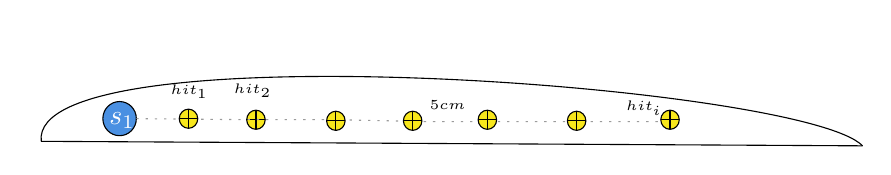
\begin{tikzpicture}[x=0.75pt,y=0.75pt,yscale=-1,xscale=1]
%uncomment if require: \path (0,300); %set diagram left start at 0, and has height of 300

%Curve Lines [id:da8422582381977624] 
\draw    (38.5,121) .. controls (32.24,66.51) and (406.04,93.84) .. (434.24,123.17) ;
%Straight Lines [id:da8049776185709991] 
\draw    (38.5,121) -- (434.24,123.17) ;
%Shape: Ellipse [id:dp7062717290883331] 
\draw  [color={rgb, 255:red, 0; green, 0; blue, 0 }  ,draw opacity=1 ][fill={rgb, 255:red, 74; green, 144; blue, 226 }  ,fill opacity=1 ] (68.2,110.06) .. controls (68.2,105.51) and (71.81,101.83) .. (76.26,101.83) .. controls (80.71,101.83) and (84.32,105.51) .. (84.32,110.06) .. controls (84.32,114.6) and (80.71,118.28) .. (76.26,118.28) .. controls (71.81,118.28) and (68.2,114.6) .. (68.2,110.06) -- cycle ;
\draw  [fill={rgb, 255:red, 248; green, 231; blue, 28 }  ,fill opacity=1 ] (137.5,110.61) .. controls (137.5,108.06) and (139.5,106) .. (141.96,106) .. controls (144.42,106) and (146.41,108.06) .. (146.41,110.61) .. controls (146.41,113.15) and (144.42,115.22) .. (141.96,115.22) .. controls (139.5,115.22) and (137.5,113.15) .. (137.5,110.61) -- cycle ; \draw   (137.5,110.61) -- (146.41,110.61) ; \draw   (141.96,106) -- (141.96,115.22) ;
%Straight Lines [id:da6986266442320166] 
\draw [color={rgb, 255:red, 155; green, 155; blue, 155 }  ,draw opacity=1 ] [dash pattern={on 0.84pt off 2.51pt}]  (84.32,110.06) -- (133.33,110.54) -- (178.33,110.54) -- (223.35,111.48) -- (278.83,111.54) -- (330.85,111.48) -- (337.85,111.48) ;
\draw  [fill={rgb, 255:red, 248; green, 231; blue, 28 }  ,fill opacity=1 ] (105,110.11) .. controls (105,107.56) and (107,105.5) .. (109.46,105.5) .. controls (111.92,105.5) and (113.91,107.56) .. (113.91,110.11) .. controls (113.91,112.65) and (111.92,114.72) .. (109.46,114.72) .. controls (107,114.72) and (105,112.65) .. (105,110.11) -- cycle ; \draw   (105,110.11) -- (113.91,110.11) ; \draw   (109.46,105.5) -- (109.46,114.72) ;
\draw  [fill={rgb, 255:red, 248; green, 231; blue, 28 }  ,fill opacity=1 ] (213,111.11) .. controls (213,108.56) and (215,106.5) .. (217.46,106.5) .. controls (219.92,106.5) and (221.91,108.56) .. (221.91,111.11) .. controls (221.91,113.65) and (219.92,115.72) .. (217.46,115.72) .. controls (215,115.72) and (213,113.65) .. (213,111.11) -- cycle ; \draw   (213,111.11) -- (221.91,111.11) ; \draw   (217.46,106.5) -- (217.46,115.72) ;
\draw  [fill={rgb, 255:red, 248; green, 231; blue, 28 }  ,fill opacity=1 ] (292,111.11) .. controls (292,108.56) and (294,106.5) .. (296.46,106.5) .. controls (298.92,106.5) and (300.91,108.56) .. (300.91,111.11) .. controls (300.91,113.65) and (298.92,115.72) .. (296.46,115.72) .. controls (294,115.72) and (292,113.65) .. (292,111.11) -- cycle ; \draw   (292,111.11) -- (300.91,111.11) ; \draw   (296.46,106.5) -- (296.46,115.72) ;
\draw  [fill={rgb, 255:red, 248; green, 231; blue, 28 }  ,fill opacity=1 ] (337,110.61) .. controls (337,108.06) and (339,106) .. (341.46,106) .. controls (343.92,106) and (345.91,108.06) .. (345.91,110.61) .. controls (345.91,113.15) and (343.92,115.22) .. (341.46,115.22) .. controls (339,115.22) and (337,113.15) .. (337,110.61) -- cycle ; \draw   (337,110.61) -- (345.91,110.61) ; \draw   (341.46,106) -- (341.46,115.22) ;
\draw  [fill={rgb, 255:red, 248; green, 231; blue, 28 }  ,fill opacity=1 ] (249,110.61) .. controls (249,108.06) and (251,106) .. (253.46,106) .. controls (255.92,106) and (257.91,108.06) .. (257.91,110.61) .. controls (257.91,113.15) and (255.92,115.22) .. (253.46,115.22) .. controls (251,115.22) and (249,113.15) .. (249,110.61) -- cycle ; \draw   (249,110.61) -- (257.91,110.61) ; \draw   (253.46,106) -- (253.46,115.22) ;
\draw  [fill={rgb, 255:red, 248; green, 231; blue, 28 }  ,fill opacity=1 ] (176,111.11) .. controls (176,108.56) and (178,106.5) .. (180.46,106.5) .. controls (182.92,106.5) and (184.91,108.56) .. (184.91,111.11) .. controls (184.91,113.65) and (182.92,115.72) .. (180.46,115.72) .. controls (178,115.72) and (176,113.65) .. (176,111.11) -- cycle ; \draw   (176,111.11) -- (184.91,111.11) ; \draw   (180.46,106.5) -- (180.46,115.72) ;

% Text Node
\draw (70.06,105.94) node [anchor=north west][inner sep=0.75pt]  [color={rgb, 255:red, 255; green, 255; blue, 255 }  ,opacity=1 ] [align=left] {$\displaystyle s_{1}$};
% Text Node
\draw (224.5,100) node [anchor=north west][inner sep=0.75pt]  [font=\tiny] [align=left] {$\displaystyle 5cm\ $};
% Text Node
\draw (99.56,92.44) node [anchor=north west][inner sep=0.75pt]  [font=\tiny,color={rgb, 255:red, 0; green, 0; blue, 0 }  ,opacity=1 ] [align=left] {$\displaystyle hit_{1}$};
% Text Node
\draw (130.06,91.94) node [anchor=north west][inner sep=0.75pt]  [font=\tiny,color={rgb, 255:red, 0; green, 0; blue, 0 }  ,opacity=1 ] [align=left] {$\displaystyle hit_{2}$};
% Text Node
\draw (319.06,100.44) node [anchor=north west][inner sep=0.75pt]  [font=\tiny,color={rgb, 255:red, 0; green, 0; blue, 0 }  ,opacity=1 ] [align=left] {$\displaystyle hit_{i}$};


\end{tikzpicture}}
        \caption{Experiment Visualization }
        \label{fig:label}
    \end{figure}

For this study, we made a {\(7\)} marks equidistant from each other at
{\(5cm\)}, However, {\(10\)} files were recorded, which means we have a
3 files as noise.\\
There are variety of methods to eliminate noise, i have used SNR (signal
to noise ratio), and ignoring negative values which excludes the hit
{\(5,8,10\)}.

    \begin{figure}[htbp]
        \centering
        \scalebox{0.5}{%% Creator: Matplotlib, PGF backend
%%
%% To include the figure in your LaTeX document, write
%%   \input{<filename>.pgf}
%%
%% Make sure the required packages are loaded in your preamble
%%   \usepackage{pgf}
%%
%% Also ensure that all the required font packages are loaded; for instance,
%% the lmodern package is sometimes necessary when using math font.
%%   \usepackage{lmodern}
%%
%% Figures using additional raster images can only be included by \input if
%% they are in the same directory as the main LaTeX file. For loading figures
%% from other directories you can use the `import` package
%%   \usepackage{import}
%%
%% and then include the figures with
%%   \import{<path to file>}{<filename>.pgf}
%%
%% Matplotlib used the following preamble
%%
\begingroup%
\makeatletter%
\begin{pgfpicture}%
\pgfpathrectangle{\pgfpointorigin}{\pgfqpoint{10.449923in}{7.259799in}}%
\pgfusepath{use as bounding box, clip}%
\begin{pgfscope}%
\pgfsetbuttcap%
\pgfsetmiterjoin%
\definecolor{currentfill}{rgb}{1.000000,1.000000,1.000000}%
\pgfsetfillcolor{currentfill}%
\pgfsetlinewidth{0.000000pt}%
\definecolor{currentstroke}{rgb}{1.000000,1.000000,1.000000}%
\pgfsetstrokecolor{currentstroke}%
\pgfsetdash{}{0pt}%
\pgfpathmoveto{\pgfqpoint{0.000000in}{0.000000in}}%
\pgfpathlineto{\pgfqpoint{10.449923in}{0.000000in}}%
\pgfpathlineto{\pgfqpoint{10.449923in}{7.259799in}}%
\pgfpathlineto{\pgfqpoint{0.000000in}{7.259799in}}%
\pgfpathlineto{\pgfqpoint{0.000000in}{0.000000in}}%
\pgfpathclose%
\pgfusepath{fill}%
\end{pgfscope}%
\begin{pgfscope}%
\pgfsetbuttcap%
\pgfsetmiterjoin%
\definecolor{currentfill}{rgb}{1.000000,1.000000,1.000000}%
\pgfsetfillcolor{currentfill}%
\pgfsetlinewidth{0.000000pt}%
\definecolor{currentstroke}{rgb}{0.000000,0.000000,0.000000}%
\pgfsetstrokecolor{currentstroke}%
\pgfsetstrokeopacity{0.000000}%
\pgfsetdash{}{0pt}%
\pgfpathmoveto{\pgfqpoint{0.844750in}{6.437873in}}%
\pgfpathlineto{\pgfqpoint{4.939352in}{6.437873in}}%
\pgfpathlineto{\pgfqpoint{4.939352in}{6.937577in}}%
\pgfpathlineto{\pgfqpoint{0.844750in}{6.937577in}}%
\pgfpathlineto{\pgfqpoint{0.844750in}{6.437873in}}%
\pgfpathclose%
\pgfusepath{fill}%
\end{pgfscope}%
\begin{pgfscope}%
\pgfpathrectangle{\pgfqpoint{0.844750in}{6.437873in}}{\pgfqpoint{4.094602in}{0.499704in}}%
\pgfusepath{clip}%
\pgfsetrectcap%
\pgfsetroundjoin%
\pgfsetlinewidth{1.304875pt}%
\definecolor{currentstroke}{rgb}{0.690196,0.690196,0.690196}%
\pgfsetstrokecolor{currentstroke}%
\pgfsetdash{}{0pt}%
\pgfpathmoveto{\pgfqpoint{1.188996in}{6.437873in}}%
\pgfpathlineto{\pgfqpoint{1.188996in}{6.937577in}}%
\pgfusepath{stroke}%
\end{pgfscope}%
\begin{pgfscope}%
\pgfsetbuttcap%
\pgfsetroundjoin%
\definecolor{currentfill}{rgb}{0.000000,0.000000,0.000000}%
\pgfsetfillcolor{currentfill}%
\pgfsetlinewidth{1.304875pt}%
\definecolor{currentstroke}{rgb}{0.000000,0.000000,0.000000}%
\pgfsetstrokecolor{currentstroke}%
\pgfsetdash{}{0pt}%
\pgfsys@defobject{currentmarker}{\pgfqpoint{0.000000in}{-0.048611in}}{\pgfqpoint{0.000000in}{0.000000in}}{%
\pgfpathmoveto{\pgfqpoint{0.000000in}{0.000000in}}%
\pgfpathlineto{\pgfqpoint{0.000000in}{-0.048611in}}%
\pgfusepath{stroke,fill}%
}%
\begin{pgfscope}%
\pgfsys@transformshift{1.188996in}{6.437873in}%
\pgfsys@useobject{currentmarker}{}%
\end{pgfscope}%
\end{pgfscope}%
\begin{pgfscope}%
\definecolor{textcolor}{rgb}{0.000000,0.000000,0.000000}%
\pgfsetstrokecolor{textcolor}%
\pgfsetfillcolor{textcolor}%
\pgftext[x=1.188996in,y=6.262873in,,top]{\color{textcolor}\rmfamily\fontsize{13.000000}{15.600000}\selectfont \(\displaystyle {0.00045}\)}%
\end{pgfscope}%
\begin{pgfscope}%
\pgfpathrectangle{\pgfqpoint{0.844750in}{6.437873in}}{\pgfqpoint{4.094602in}{0.499704in}}%
\pgfusepath{clip}%
\pgfsetrectcap%
\pgfsetroundjoin%
\pgfsetlinewidth{1.304875pt}%
\definecolor{currentstroke}{rgb}{0.690196,0.690196,0.690196}%
\pgfsetstrokecolor{currentstroke}%
\pgfsetdash{}{0pt}%
\pgfpathmoveto{\pgfqpoint{2.097777in}{6.437873in}}%
\pgfpathlineto{\pgfqpoint{2.097777in}{6.937577in}}%
\pgfusepath{stroke}%
\end{pgfscope}%
\begin{pgfscope}%
\pgfsetbuttcap%
\pgfsetroundjoin%
\definecolor{currentfill}{rgb}{0.000000,0.000000,0.000000}%
\pgfsetfillcolor{currentfill}%
\pgfsetlinewidth{1.304875pt}%
\definecolor{currentstroke}{rgb}{0.000000,0.000000,0.000000}%
\pgfsetstrokecolor{currentstroke}%
\pgfsetdash{}{0pt}%
\pgfsys@defobject{currentmarker}{\pgfqpoint{0.000000in}{-0.048611in}}{\pgfqpoint{0.000000in}{0.000000in}}{%
\pgfpathmoveto{\pgfqpoint{0.000000in}{0.000000in}}%
\pgfpathlineto{\pgfqpoint{0.000000in}{-0.048611in}}%
\pgfusepath{stroke,fill}%
}%
\begin{pgfscope}%
\pgfsys@transformshift{2.097777in}{6.437873in}%
\pgfsys@useobject{currentmarker}{}%
\end{pgfscope}%
\end{pgfscope}%
\begin{pgfscope}%
\definecolor{textcolor}{rgb}{0.000000,0.000000,0.000000}%
\pgfsetstrokecolor{textcolor}%
\pgfsetfillcolor{textcolor}%
\pgftext[x=2.097777in,y=6.262873in,,top]{\color{textcolor}\rmfamily\fontsize{13.000000}{15.600000}\selectfont \(\displaystyle {0.00050}\)}%
\end{pgfscope}%
\begin{pgfscope}%
\pgfpathrectangle{\pgfqpoint{0.844750in}{6.437873in}}{\pgfqpoint{4.094602in}{0.499704in}}%
\pgfusepath{clip}%
\pgfsetrectcap%
\pgfsetroundjoin%
\pgfsetlinewidth{1.304875pt}%
\definecolor{currentstroke}{rgb}{0.690196,0.690196,0.690196}%
\pgfsetstrokecolor{currentstroke}%
\pgfsetdash{}{0pt}%
\pgfpathmoveto{\pgfqpoint{3.006558in}{6.437873in}}%
\pgfpathlineto{\pgfqpoint{3.006558in}{6.937577in}}%
\pgfusepath{stroke}%
\end{pgfscope}%
\begin{pgfscope}%
\pgfsetbuttcap%
\pgfsetroundjoin%
\definecolor{currentfill}{rgb}{0.000000,0.000000,0.000000}%
\pgfsetfillcolor{currentfill}%
\pgfsetlinewidth{1.304875pt}%
\definecolor{currentstroke}{rgb}{0.000000,0.000000,0.000000}%
\pgfsetstrokecolor{currentstroke}%
\pgfsetdash{}{0pt}%
\pgfsys@defobject{currentmarker}{\pgfqpoint{0.000000in}{-0.048611in}}{\pgfqpoint{0.000000in}{0.000000in}}{%
\pgfpathmoveto{\pgfqpoint{0.000000in}{0.000000in}}%
\pgfpathlineto{\pgfqpoint{0.000000in}{-0.048611in}}%
\pgfusepath{stroke,fill}%
}%
\begin{pgfscope}%
\pgfsys@transformshift{3.006558in}{6.437873in}%
\pgfsys@useobject{currentmarker}{}%
\end{pgfscope}%
\end{pgfscope}%
\begin{pgfscope}%
\definecolor{textcolor}{rgb}{0.000000,0.000000,0.000000}%
\pgfsetstrokecolor{textcolor}%
\pgfsetfillcolor{textcolor}%
\pgftext[x=3.006558in,y=6.262873in,,top]{\color{textcolor}\rmfamily\fontsize{13.000000}{15.600000}\selectfont \(\displaystyle {0.00055}\)}%
\end{pgfscope}%
\begin{pgfscope}%
\pgfpathrectangle{\pgfqpoint{0.844750in}{6.437873in}}{\pgfqpoint{4.094602in}{0.499704in}}%
\pgfusepath{clip}%
\pgfsetrectcap%
\pgfsetroundjoin%
\pgfsetlinewidth{1.304875pt}%
\definecolor{currentstroke}{rgb}{0.690196,0.690196,0.690196}%
\pgfsetstrokecolor{currentstroke}%
\pgfsetdash{}{0pt}%
\pgfpathmoveto{\pgfqpoint{3.915338in}{6.437873in}}%
\pgfpathlineto{\pgfqpoint{3.915338in}{6.937577in}}%
\pgfusepath{stroke}%
\end{pgfscope}%
\begin{pgfscope}%
\pgfsetbuttcap%
\pgfsetroundjoin%
\definecolor{currentfill}{rgb}{0.000000,0.000000,0.000000}%
\pgfsetfillcolor{currentfill}%
\pgfsetlinewidth{1.304875pt}%
\definecolor{currentstroke}{rgb}{0.000000,0.000000,0.000000}%
\pgfsetstrokecolor{currentstroke}%
\pgfsetdash{}{0pt}%
\pgfsys@defobject{currentmarker}{\pgfqpoint{0.000000in}{-0.048611in}}{\pgfqpoint{0.000000in}{0.000000in}}{%
\pgfpathmoveto{\pgfqpoint{0.000000in}{0.000000in}}%
\pgfpathlineto{\pgfqpoint{0.000000in}{-0.048611in}}%
\pgfusepath{stroke,fill}%
}%
\begin{pgfscope}%
\pgfsys@transformshift{3.915338in}{6.437873in}%
\pgfsys@useobject{currentmarker}{}%
\end{pgfscope}%
\end{pgfscope}%
\begin{pgfscope}%
\definecolor{textcolor}{rgb}{0.000000,0.000000,0.000000}%
\pgfsetstrokecolor{textcolor}%
\pgfsetfillcolor{textcolor}%
\pgftext[x=3.915338in,y=6.262873in,,top]{\color{textcolor}\rmfamily\fontsize{13.000000}{15.600000}\selectfont \(\displaystyle {0.00060}\)}%
\end{pgfscope}%
\begin{pgfscope}%
\pgfpathrectangle{\pgfqpoint{0.844750in}{6.437873in}}{\pgfqpoint{4.094602in}{0.499704in}}%
\pgfusepath{clip}%
\pgfsetrectcap%
\pgfsetroundjoin%
\pgfsetlinewidth{1.304875pt}%
\definecolor{currentstroke}{rgb}{0.690196,0.690196,0.690196}%
\pgfsetstrokecolor{currentstroke}%
\pgfsetdash{}{0pt}%
\pgfpathmoveto{\pgfqpoint{4.824119in}{6.437873in}}%
\pgfpathlineto{\pgfqpoint{4.824119in}{6.937577in}}%
\pgfusepath{stroke}%
\end{pgfscope}%
\begin{pgfscope}%
\pgfsetbuttcap%
\pgfsetroundjoin%
\definecolor{currentfill}{rgb}{0.000000,0.000000,0.000000}%
\pgfsetfillcolor{currentfill}%
\pgfsetlinewidth{1.304875pt}%
\definecolor{currentstroke}{rgb}{0.000000,0.000000,0.000000}%
\pgfsetstrokecolor{currentstroke}%
\pgfsetdash{}{0pt}%
\pgfsys@defobject{currentmarker}{\pgfqpoint{0.000000in}{-0.048611in}}{\pgfqpoint{0.000000in}{0.000000in}}{%
\pgfpathmoveto{\pgfqpoint{0.000000in}{0.000000in}}%
\pgfpathlineto{\pgfqpoint{0.000000in}{-0.048611in}}%
\pgfusepath{stroke,fill}%
}%
\begin{pgfscope}%
\pgfsys@transformshift{4.824119in}{6.437873in}%
\pgfsys@useobject{currentmarker}{}%
\end{pgfscope}%
\end{pgfscope}%
\begin{pgfscope}%
\definecolor{textcolor}{rgb}{0.000000,0.000000,0.000000}%
\pgfsetstrokecolor{textcolor}%
\pgfsetfillcolor{textcolor}%
\pgftext[x=4.824119in,y=6.262873in,,top]{\color{textcolor}\rmfamily\fontsize{13.000000}{15.600000}\selectfont \(\displaystyle {0.00065}\)}%
\end{pgfscope}%
\begin{pgfscope}%
\definecolor{textcolor}{rgb}{0.000000,0.000000,0.000000}%
\pgfsetstrokecolor{textcolor}%
\pgfsetfillcolor{textcolor}%
\pgftext[x=4.939352in,y=6.073059in,right,top]{\color{textcolor}\rmfamily\fontsize{13.000000}{15.600000}\selectfont \(\displaystyle {+8.402}\)}%
\end{pgfscope}%
\begin{pgfscope}%
\pgfpathrectangle{\pgfqpoint{0.844750in}{6.437873in}}{\pgfqpoint{4.094602in}{0.499704in}}%
\pgfusepath{clip}%
\pgfsetrectcap%
\pgfsetroundjoin%
\pgfsetlinewidth{1.304875pt}%
\definecolor{currentstroke}{rgb}{0.690196,0.690196,0.690196}%
\pgfsetstrokecolor{currentstroke}%
\pgfsetdash{}{0pt}%
\pgfpathmoveto{\pgfqpoint{0.844750in}{6.489938in}}%
\pgfpathlineto{\pgfqpoint{4.939352in}{6.489938in}}%
\pgfusepath{stroke}%
\end{pgfscope}%
\begin{pgfscope}%
\pgfsetbuttcap%
\pgfsetroundjoin%
\definecolor{currentfill}{rgb}{0.000000,0.000000,0.000000}%
\pgfsetfillcolor{currentfill}%
\pgfsetlinewidth{1.304875pt}%
\definecolor{currentstroke}{rgb}{0.000000,0.000000,0.000000}%
\pgfsetstrokecolor{currentstroke}%
\pgfsetdash{}{0pt}%
\pgfsys@defobject{currentmarker}{\pgfqpoint{-0.048611in}{0.000000in}}{\pgfqpoint{-0.000000in}{0.000000in}}{%
\pgfpathmoveto{\pgfqpoint{-0.000000in}{0.000000in}}%
\pgfpathlineto{\pgfqpoint{-0.048611in}{0.000000in}}%
\pgfusepath{stroke,fill}%
}%
\begin{pgfscope}%
\pgfsys@transformshift{0.844750in}{6.489938in}%
\pgfsys@useobject{currentmarker}{}%
\end{pgfscope}%
\end{pgfscope}%
\begin{pgfscope}%
\definecolor{textcolor}{rgb}{0.000000,0.000000,0.000000}%
\pgfsetstrokecolor{textcolor}%
\pgfsetfillcolor{textcolor}%
\pgftext[x=0.250000in, y=6.432068in, left, base]{\color{textcolor}\rmfamily\fontsize{13.000000}{15.600000}\selectfont \(\displaystyle {\ensuremath{-}0.02}\)}%
\end{pgfscope}%
\begin{pgfscope}%
\pgfpathrectangle{\pgfqpoint{0.844750in}{6.437873in}}{\pgfqpoint{4.094602in}{0.499704in}}%
\pgfusepath{clip}%
\pgfsetrectcap%
\pgfsetroundjoin%
\pgfsetlinewidth{1.304875pt}%
\definecolor{currentstroke}{rgb}{0.690196,0.690196,0.690196}%
\pgfsetstrokecolor{currentstroke}%
\pgfsetdash{}{0pt}%
\pgfpathmoveto{\pgfqpoint{0.844750in}{6.717201in}}%
\pgfpathlineto{\pgfqpoint{4.939352in}{6.717201in}}%
\pgfusepath{stroke}%
\end{pgfscope}%
\begin{pgfscope}%
\pgfsetbuttcap%
\pgfsetroundjoin%
\definecolor{currentfill}{rgb}{0.000000,0.000000,0.000000}%
\pgfsetfillcolor{currentfill}%
\pgfsetlinewidth{1.304875pt}%
\definecolor{currentstroke}{rgb}{0.000000,0.000000,0.000000}%
\pgfsetstrokecolor{currentstroke}%
\pgfsetdash{}{0pt}%
\pgfsys@defobject{currentmarker}{\pgfqpoint{-0.048611in}{0.000000in}}{\pgfqpoint{-0.000000in}{0.000000in}}{%
\pgfpathmoveto{\pgfqpoint{-0.000000in}{0.000000in}}%
\pgfpathlineto{\pgfqpoint{-0.048611in}{0.000000in}}%
\pgfusepath{stroke,fill}%
}%
\begin{pgfscope}%
\pgfsys@transformshift{0.844750in}{6.717201in}%
\pgfsys@useobject{currentmarker}{}%
\end{pgfscope}%
\end{pgfscope}%
\begin{pgfscope}%
\definecolor{textcolor}{rgb}{0.000000,0.000000,0.000000}%
\pgfsetstrokecolor{textcolor}%
\pgfsetfillcolor{textcolor}%
\pgftext[x=0.379630in, y=6.659331in, left, base]{\color{textcolor}\rmfamily\fontsize{13.000000}{15.600000}\selectfont \(\displaystyle {0.00}\)}%
\end{pgfscope}%
\begin{pgfscope}%
\pgfpathrectangle{\pgfqpoint{0.844750in}{6.437873in}}{\pgfqpoint{4.094602in}{0.499704in}}%
\pgfusepath{clip}%
\pgfsetrectcap%
\pgfsetroundjoin%
\pgfsetlinewidth{1.003750pt}%
\definecolor{currentstroke}{rgb}{0.000000,0.000000,1.000000}%
\pgfsetstrokecolor{currentstroke}%
\pgfsetdash{}{0pt}%
\pgfpathmoveto{\pgfqpoint{1.030869in}{6.627039in}}%
\pgfpathlineto{\pgfqpoint{1.034507in}{6.623571in}}%
\pgfpathlineto{\pgfqpoint{1.038146in}{6.623571in}}%
\pgfpathlineto{\pgfqpoint{1.041785in}{6.627039in}}%
\pgfpathlineto{\pgfqpoint{1.045423in}{6.633975in}}%
\pgfpathlineto{\pgfqpoint{1.049062in}{6.637443in}}%
\pgfpathlineto{\pgfqpoint{1.056339in}{6.651314in}}%
\pgfpathlineto{\pgfqpoint{1.063617in}{6.675588in}}%
\pgfpathlineto{\pgfqpoint{1.067255in}{6.679056in}}%
\pgfpathlineto{\pgfqpoint{1.070894in}{6.685991in}}%
\pgfpathlineto{\pgfqpoint{1.089087in}{6.738007in}}%
\pgfpathlineto{\pgfqpoint{1.096365in}{6.744943in}}%
\pgfpathlineto{\pgfqpoint{1.100004in}{6.751879in}}%
\pgfpathlineto{\pgfqpoint{1.103642in}{6.765750in}}%
\pgfpathlineto{\pgfqpoint{1.107281in}{6.772685in}}%
\pgfpathlineto{\pgfqpoint{1.110920in}{6.783088in}}%
\pgfpathlineto{\pgfqpoint{1.114558in}{6.790024in}}%
\pgfpathlineto{\pgfqpoint{1.118197in}{6.793492in}}%
\pgfpathlineto{\pgfqpoint{1.121836in}{6.793492in}}%
\pgfpathlineto{\pgfqpoint{1.125474in}{6.800427in}}%
\pgfpathlineto{\pgfqpoint{1.129113in}{6.810831in}}%
\pgfpathlineto{\pgfqpoint{1.136390in}{6.824702in}}%
\pgfpathlineto{\pgfqpoint{1.140029in}{6.824702in}}%
\pgfpathlineto{\pgfqpoint{1.143668in}{6.831637in}}%
\pgfpathlineto{\pgfqpoint{1.147306in}{6.842040in}}%
\pgfpathlineto{\pgfqpoint{1.161861in}{6.869782in}}%
\pgfpathlineto{\pgfqpoint{1.165500in}{6.880186in}}%
\pgfpathlineto{\pgfqpoint{1.176416in}{6.900992in}}%
\pgfpathlineto{\pgfqpoint{1.190970in}{6.914863in}}%
\pgfpathlineto{\pgfqpoint{1.194609in}{6.914863in}}%
\pgfpathlineto{\pgfqpoint{1.198248in}{6.907928in}}%
\pgfpathlineto{\pgfqpoint{1.205525in}{6.914863in}}%
\pgfpathlineto{\pgfqpoint{1.209164in}{6.914863in}}%
\pgfpathlineto{\pgfqpoint{1.216441in}{6.907928in}}%
\pgfpathlineto{\pgfqpoint{1.220080in}{6.907928in}}%
\pgfpathlineto{\pgfqpoint{1.223718in}{6.904460in}}%
\pgfpathlineto{\pgfqpoint{1.227357in}{6.897525in}}%
\pgfpathlineto{\pgfqpoint{1.230996in}{6.894057in}}%
\pgfpathlineto{\pgfqpoint{1.238273in}{6.894057in}}%
\pgfpathlineto{\pgfqpoint{1.241912in}{6.890589in}}%
\pgfpathlineto{\pgfqpoint{1.245551in}{6.890589in}}%
\pgfpathlineto{\pgfqpoint{1.249189in}{6.883654in}}%
\pgfpathlineto{\pgfqpoint{1.260105in}{6.873250in}}%
\pgfpathlineto{\pgfqpoint{1.263744in}{6.866315in}}%
\pgfpathlineto{\pgfqpoint{1.267383in}{6.862847in}}%
\pgfpathlineto{\pgfqpoint{1.274660in}{6.848976in}}%
\pgfpathlineto{\pgfqpoint{1.278299in}{6.838573in}}%
\pgfpathlineto{\pgfqpoint{1.285576in}{6.831637in}}%
\pgfpathlineto{\pgfqpoint{1.292853in}{6.807363in}}%
\pgfpathlineto{\pgfqpoint{1.296492in}{6.796959in}}%
\pgfpathlineto{\pgfqpoint{1.300131in}{6.790024in}}%
\pgfpathlineto{\pgfqpoint{1.318324in}{6.724136in}}%
\pgfpathlineto{\pgfqpoint{1.321963in}{6.713733in}}%
\pgfpathlineto{\pgfqpoint{1.354711in}{6.592362in}}%
\pgfpathlineto{\pgfqpoint{1.358349in}{6.581958in}}%
\pgfpathlineto{\pgfqpoint{1.361988in}{6.575023in}}%
\pgfpathlineto{\pgfqpoint{1.365627in}{6.564620in}}%
\pgfpathlineto{\pgfqpoint{1.376543in}{6.526474in}}%
\pgfpathlineto{\pgfqpoint{1.380182in}{6.516071in}}%
\pgfpathlineto{\pgfqpoint{1.387459in}{6.502200in}}%
\pgfpathlineto{\pgfqpoint{1.394736in}{6.495264in}}%
\pgfpathlineto{\pgfqpoint{1.398375in}{6.488329in}}%
\pgfpathlineto{\pgfqpoint{1.405652in}{6.481393in}}%
\pgfpathlineto{\pgfqpoint{1.409291in}{6.481393in}}%
\pgfpathlineto{\pgfqpoint{1.416568in}{6.474458in}}%
\pgfpathlineto{\pgfqpoint{1.420207in}{6.467522in}}%
\pgfpathlineto{\pgfqpoint{1.427484in}{6.460587in}}%
\pgfpathlineto{\pgfqpoint{1.431123in}{6.460587in}}%
\pgfpathlineto{\pgfqpoint{1.434762in}{6.467522in}}%
\pgfpathlineto{\pgfqpoint{1.445678in}{6.467522in}}%
\pgfpathlineto{\pgfqpoint{1.449316in}{6.470990in}}%
\pgfpathlineto{\pgfqpoint{1.452955in}{6.477925in}}%
\pgfpathlineto{\pgfqpoint{1.456594in}{6.481393in}}%
\pgfpathlineto{\pgfqpoint{1.460232in}{6.481393in}}%
\pgfpathlineto{\pgfqpoint{1.474787in}{6.509135in}}%
\pgfpathlineto{\pgfqpoint{1.478426in}{6.512603in}}%
\pgfpathlineto{\pgfqpoint{1.482064in}{6.512603in}}%
\pgfpathlineto{\pgfqpoint{1.485703in}{6.509135in}}%
\pgfpathlineto{\pgfqpoint{1.489342in}{6.516071in}}%
\pgfpathlineto{\pgfqpoint{1.500258in}{6.526474in}}%
\pgfpathlineto{\pgfqpoint{1.503896in}{6.526474in}}%
\pgfpathlineto{\pgfqpoint{1.507535in}{6.533410in}}%
\pgfpathlineto{\pgfqpoint{1.511174in}{6.543813in}}%
\pgfpathlineto{\pgfqpoint{1.514813in}{6.550748in}}%
\pgfpathlineto{\pgfqpoint{1.518451in}{6.561152in}}%
\pgfpathlineto{\pgfqpoint{1.522090in}{6.561152in}}%
\pgfpathlineto{\pgfqpoint{1.525729in}{6.564620in}}%
\pgfpathlineto{\pgfqpoint{1.547561in}{6.606233in}}%
\pgfpathlineto{\pgfqpoint{1.551199in}{6.606233in}}%
\pgfpathlineto{\pgfqpoint{1.554838in}{6.613168in}}%
\pgfpathlineto{\pgfqpoint{1.558477in}{6.616636in}}%
\pgfpathlineto{\pgfqpoint{1.573031in}{6.644378in}}%
\pgfpathlineto{\pgfqpoint{1.576670in}{6.654781in}}%
\pgfpathlineto{\pgfqpoint{1.580309in}{6.661717in}}%
\pgfpathlineto{\pgfqpoint{1.583947in}{6.665185in}}%
\pgfpathlineto{\pgfqpoint{1.591225in}{6.679056in}}%
\pgfpathlineto{\pgfqpoint{1.594863in}{6.692927in}}%
\pgfpathlineto{\pgfqpoint{1.598502in}{6.699862in}}%
\pgfpathlineto{\pgfqpoint{1.602141in}{6.710265in}}%
\pgfpathlineto{\pgfqpoint{1.605779in}{6.717201in}}%
\pgfpathlineto{\pgfqpoint{1.609418in}{6.727604in}}%
\pgfpathlineto{\pgfqpoint{1.613057in}{6.734540in}}%
\pgfpathlineto{\pgfqpoint{1.616695in}{6.738007in}}%
\pgfpathlineto{\pgfqpoint{1.623973in}{6.758814in}}%
\pgfpathlineto{\pgfqpoint{1.627611in}{6.772685in}}%
\pgfpathlineto{\pgfqpoint{1.634889in}{6.779621in}}%
\pgfpathlineto{\pgfqpoint{1.638527in}{6.786556in}}%
\pgfpathlineto{\pgfqpoint{1.645805in}{6.810831in}}%
\pgfpathlineto{\pgfqpoint{1.660360in}{6.824702in}}%
\pgfpathlineto{\pgfqpoint{1.663998in}{6.831637in}}%
\pgfpathlineto{\pgfqpoint{1.667637in}{6.842040in}}%
\pgfpathlineto{\pgfqpoint{1.671276in}{6.845508in}}%
\pgfpathlineto{\pgfqpoint{1.678553in}{6.845508in}}%
\pgfpathlineto{\pgfqpoint{1.685830in}{6.852444in}}%
\pgfpathlineto{\pgfqpoint{1.689469in}{6.845508in}}%
\pgfpathlineto{\pgfqpoint{1.693108in}{6.845508in}}%
\pgfpathlineto{\pgfqpoint{1.707662in}{6.859379in}}%
\pgfpathlineto{\pgfqpoint{1.714940in}{6.859379in}}%
\pgfpathlineto{\pgfqpoint{1.718578in}{6.862847in}}%
\pgfpathlineto{\pgfqpoint{1.722217in}{6.855911in}}%
\pgfpathlineto{\pgfqpoint{1.733133in}{6.855911in}}%
\pgfpathlineto{\pgfqpoint{1.736772in}{6.848976in}}%
\pgfpathlineto{\pgfqpoint{1.740410in}{6.848976in}}%
\pgfpathlineto{\pgfqpoint{1.744049in}{6.845508in}}%
\pgfpathlineto{\pgfqpoint{1.751326in}{6.845508in}}%
\pgfpathlineto{\pgfqpoint{1.758604in}{6.838573in}}%
\pgfpathlineto{\pgfqpoint{1.762242in}{6.831637in}}%
\pgfpathlineto{\pgfqpoint{1.769520in}{6.824702in}}%
\pgfpathlineto{\pgfqpoint{1.802268in}{6.824702in}}%
\pgfpathlineto{\pgfqpoint{1.805907in}{6.821234in}}%
\pgfpathlineto{\pgfqpoint{1.816823in}{6.821234in}}%
\pgfpathlineto{\pgfqpoint{1.820461in}{6.824702in}}%
\pgfpathlineto{\pgfqpoint{1.827739in}{6.824702in}}%
\pgfpathlineto{\pgfqpoint{1.831377in}{6.821234in}}%
\pgfpathlineto{\pgfqpoint{1.835016in}{6.821234in}}%
\pgfpathlineto{\pgfqpoint{1.838655in}{6.817766in}}%
\pgfpathlineto{\pgfqpoint{1.842293in}{6.821234in}}%
\pgfpathlineto{\pgfqpoint{1.849571in}{6.814298in}}%
\pgfpathlineto{\pgfqpoint{1.856848in}{6.800427in}}%
\pgfpathlineto{\pgfqpoint{1.864125in}{6.793492in}}%
\pgfpathlineto{\pgfqpoint{1.871403in}{6.779621in}}%
\pgfpathlineto{\pgfqpoint{1.875041in}{6.776153in}}%
\pgfpathlineto{\pgfqpoint{1.878680in}{6.769217in}}%
\pgfpathlineto{\pgfqpoint{1.885957in}{6.744943in}}%
\pgfpathlineto{\pgfqpoint{1.907789in}{6.724136in}}%
\pgfpathlineto{\pgfqpoint{1.911428in}{6.713733in}}%
\pgfpathlineto{\pgfqpoint{1.915067in}{6.710265in}}%
\pgfpathlineto{\pgfqpoint{1.918706in}{6.710265in}}%
\pgfpathlineto{\pgfqpoint{1.922344in}{6.706798in}}%
\pgfpathlineto{\pgfqpoint{1.925983in}{6.696394in}}%
\pgfpathlineto{\pgfqpoint{1.929622in}{6.689459in}}%
\pgfpathlineto{\pgfqpoint{1.933260in}{6.685991in}}%
\pgfpathlineto{\pgfqpoint{1.940538in}{6.685991in}}%
\pgfpathlineto{\pgfqpoint{1.944176in}{6.682523in}}%
\pgfpathlineto{\pgfqpoint{1.951454in}{6.668652in}}%
\pgfpathlineto{\pgfqpoint{1.962370in}{6.679056in}}%
\pgfpathlineto{\pgfqpoint{1.966008in}{6.675588in}}%
\pgfpathlineto{\pgfqpoint{1.969647in}{6.675588in}}%
\pgfpathlineto{\pgfqpoint{1.973286in}{6.672120in}}%
\pgfpathlineto{\pgfqpoint{1.976924in}{6.672120in}}%
\pgfpathlineto{\pgfqpoint{1.980563in}{6.668652in}}%
\pgfpathlineto{\pgfqpoint{1.984202in}{6.668652in}}%
\pgfpathlineto{\pgfqpoint{1.987840in}{6.672120in}}%
\pgfpathlineto{\pgfqpoint{1.991479in}{6.672120in}}%
\pgfpathlineto{\pgfqpoint{1.995118in}{6.665185in}}%
\pgfpathlineto{\pgfqpoint{1.998756in}{6.661717in}}%
\pgfpathlineto{\pgfqpoint{2.002395in}{6.661717in}}%
\pgfpathlineto{\pgfqpoint{2.006034in}{6.665185in}}%
\pgfpathlineto{\pgfqpoint{2.009672in}{6.672120in}}%
\pgfpathlineto{\pgfqpoint{2.013311in}{6.675588in}}%
\pgfpathlineto{\pgfqpoint{2.016950in}{6.672120in}}%
\pgfpathlineto{\pgfqpoint{2.020588in}{6.675588in}}%
\pgfpathlineto{\pgfqpoint{2.024227in}{6.675588in}}%
\pgfpathlineto{\pgfqpoint{2.027866in}{6.679056in}}%
\pgfpathlineto{\pgfqpoint{2.031504in}{6.679056in}}%
\pgfpathlineto{\pgfqpoint{2.038782in}{6.665185in}}%
\pgfpathlineto{\pgfqpoint{2.053337in}{6.665185in}}%
\pgfpathlineto{\pgfqpoint{2.056975in}{6.668652in}}%
\pgfpathlineto{\pgfqpoint{2.060614in}{6.668652in}}%
\pgfpathlineto{\pgfqpoint{2.064253in}{6.665185in}}%
\pgfpathlineto{\pgfqpoint{2.071530in}{6.672120in}}%
\pgfpathlineto{\pgfqpoint{2.075169in}{6.672120in}}%
\pgfpathlineto{\pgfqpoint{2.078807in}{6.668652in}}%
\pgfpathlineto{\pgfqpoint{2.082446in}{6.672120in}}%
\pgfpathlineto{\pgfqpoint{2.086085in}{6.672120in}}%
\pgfpathlineto{\pgfqpoint{2.089723in}{6.675588in}}%
\pgfpathlineto{\pgfqpoint{2.093362in}{6.675588in}}%
\pgfpathlineto{\pgfqpoint{2.097001in}{6.672120in}}%
\pgfpathlineto{\pgfqpoint{2.100639in}{6.675588in}}%
\pgfpathlineto{\pgfqpoint{2.104278in}{6.675588in}}%
\pgfpathlineto{\pgfqpoint{2.107917in}{6.679056in}}%
\pgfpathlineto{\pgfqpoint{2.118833in}{6.668652in}}%
\pgfpathlineto{\pgfqpoint{2.126110in}{6.675588in}}%
\pgfpathlineto{\pgfqpoint{2.137026in}{6.675588in}}%
\pgfpathlineto{\pgfqpoint{2.140665in}{6.679056in}}%
\pgfpathlineto{\pgfqpoint{2.144303in}{6.679056in}}%
\pgfpathlineto{\pgfqpoint{2.147942in}{6.682523in}}%
\pgfpathlineto{\pgfqpoint{2.155219in}{6.682523in}}%
\pgfpathlineto{\pgfqpoint{2.158858in}{6.679056in}}%
\pgfpathlineto{\pgfqpoint{2.166135in}{6.685991in}}%
\pgfpathlineto{\pgfqpoint{2.169774in}{6.685991in}}%
\pgfpathlineto{\pgfqpoint{2.184329in}{6.699862in}}%
\pgfpathlineto{\pgfqpoint{2.191606in}{6.699862in}}%
\pgfpathlineto{\pgfqpoint{2.195245in}{6.703330in}}%
\pgfpathlineto{\pgfqpoint{2.198884in}{6.713733in}}%
\pgfpathlineto{\pgfqpoint{2.202522in}{6.720669in}}%
\pgfpathlineto{\pgfqpoint{2.213438in}{6.731072in}}%
\pgfpathlineto{\pgfqpoint{2.220716in}{6.744943in}}%
\pgfpathlineto{\pgfqpoint{2.224354in}{6.748411in}}%
\pgfpathlineto{\pgfqpoint{2.227993in}{6.748411in}}%
\pgfpathlineto{\pgfqpoint{2.231632in}{6.744943in}}%
\pgfpathlineto{\pgfqpoint{2.235270in}{6.744943in}}%
\pgfpathlineto{\pgfqpoint{2.238909in}{6.751879in}}%
\pgfpathlineto{\pgfqpoint{2.242548in}{6.755346in}}%
\pgfpathlineto{\pgfqpoint{2.246186in}{6.762282in}}%
\pgfpathlineto{\pgfqpoint{2.249825in}{6.765750in}}%
\pgfpathlineto{\pgfqpoint{2.253464in}{6.765750in}}%
\pgfpathlineto{\pgfqpoint{2.257102in}{6.762282in}}%
\pgfpathlineto{\pgfqpoint{2.260741in}{6.762282in}}%
\pgfpathlineto{\pgfqpoint{2.264380in}{6.769217in}}%
\pgfpathlineto{\pgfqpoint{2.271657in}{6.769217in}}%
\pgfpathlineto{\pgfqpoint{2.275296in}{6.762282in}}%
\pgfpathlineto{\pgfqpoint{2.282573in}{6.762282in}}%
\pgfpathlineto{\pgfqpoint{2.286212in}{6.765750in}}%
\pgfpathlineto{\pgfqpoint{2.289850in}{6.762282in}}%
\pgfpathlineto{\pgfqpoint{2.297128in}{6.762282in}}%
\pgfpathlineto{\pgfqpoint{2.311682in}{6.748411in}}%
\pgfpathlineto{\pgfqpoint{2.315321in}{6.748411in}}%
\pgfpathlineto{\pgfqpoint{2.318960in}{6.744943in}}%
\pgfpathlineto{\pgfqpoint{2.333515in}{6.744943in}}%
\pgfpathlineto{\pgfqpoint{2.337153in}{6.741475in}}%
\pgfpathlineto{\pgfqpoint{2.340792in}{6.741475in}}%
\pgfpathlineto{\pgfqpoint{2.348069in}{6.748411in}}%
\pgfpathlineto{\pgfqpoint{2.351708in}{6.744943in}}%
\pgfpathlineto{\pgfqpoint{2.355347in}{6.744943in}}%
\pgfpathlineto{\pgfqpoint{2.358985in}{6.741475in}}%
\pgfpathlineto{\pgfqpoint{2.362624in}{6.741475in}}%
\pgfpathlineto{\pgfqpoint{2.366263in}{6.744943in}}%
\pgfpathlineto{\pgfqpoint{2.369901in}{6.744943in}}%
\pgfpathlineto{\pgfqpoint{2.377179in}{6.751879in}}%
\pgfpathlineto{\pgfqpoint{2.380817in}{6.744943in}}%
\pgfpathlineto{\pgfqpoint{2.384456in}{6.741475in}}%
\pgfpathlineto{\pgfqpoint{2.388095in}{6.744943in}}%
\pgfpathlineto{\pgfqpoint{2.395372in}{6.738007in}}%
\pgfpathlineto{\pgfqpoint{2.399011in}{6.738007in}}%
\pgfpathlineto{\pgfqpoint{2.402649in}{6.731072in}}%
\pgfpathlineto{\pgfqpoint{2.409927in}{6.731072in}}%
\pgfpathlineto{\pgfqpoint{2.413565in}{6.727604in}}%
\pgfpathlineto{\pgfqpoint{2.417204in}{6.727604in}}%
\pgfpathlineto{\pgfqpoint{2.420843in}{6.720669in}}%
\pgfpathlineto{\pgfqpoint{2.424481in}{6.720669in}}%
\pgfpathlineto{\pgfqpoint{2.431759in}{6.713733in}}%
\pgfpathlineto{\pgfqpoint{2.435397in}{6.706798in}}%
\pgfpathlineto{\pgfqpoint{2.439036in}{6.703330in}}%
\pgfpathlineto{\pgfqpoint{2.442675in}{6.703330in}}%
\pgfpathlineto{\pgfqpoint{2.446313in}{6.706798in}}%
\pgfpathlineto{\pgfqpoint{2.449952in}{6.706798in}}%
\pgfpathlineto{\pgfqpoint{2.453591in}{6.703330in}}%
\pgfpathlineto{\pgfqpoint{2.457229in}{6.703330in}}%
\pgfpathlineto{\pgfqpoint{2.460868in}{6.699862in}}%
\pgfpathlineto{\pgfqpoint{2.464507in}{6.699862in}}%
\pgfpathlineto{\pgfqpoint{2.468146in}{6.696394in}}%
\pgfpathlineto{\pgfqpoint{2.471784in}{6.689459in}}%
\pgfpathlineto{\pgfqpoint{2.475423in}{6.689459in}}%
\pgfpathlineto{\pgfqpoint{2.479062in}{6.692927in}}%
\pgfpathlineto{\pgfqpoint{2.486339in}{6.692927in}}%
\pgfpathlineto{\pgfqpoint{2.504532in}{6.675588in}}%
\pgfpathlineto{\pgfqpoint{2.511810in}{6.675588in}}%
\pgfpathlineto{\pgfqpoint{2.515448in}{6.679056in}}%
\pgfpathlineto{\pgfqpoint{2.522726in}{6.679056in}}%
\pgfpathlineto{\pgfqpoint{2.526364in}{6.682523in}}%
\pgfpathlineto{\pgfqpoint{2.530003in}{6.679056in}}%
\pgfpathlineto{\pgfqpoint{2.533642in}{6.679056in}}%
\pgfpathlineto{\pgfqpoint{2.540919in}{6.685991in}}%
\pgfpathlineto{\pgfqpoint{2.548196in}{6.679056in}}%
\pgfpathlineto{\pgfqpoint{2.555474in}{6.685991in}}%
\pgfpathlineto{\pgfqpoint{2.559112in}{6.692927in}}%
\pgfpathlineto{\pgfqpoint{2.562751in}{6.696394in}}%
\pgfpathlineto{\pgfqpoint{2.573667in}{6.696394in}}%
\pgfpathlineto{\pgfqpoint{2.577306in}{6.699862in}}%
\pgfpathlineto{\pgfqpoint{2.588222in}{6.699862in}}%
\pgfpathlineto{\pgfqpoint{2.595499in}{6.706798in}}%
\pgfpathlineto{\pgfqpoint{2.602777in}{6.706798in}}%
\pgfpathlineto{\pgfqpoint{2.613693in}{6.717201in}}%
\pgfpathlineto{\pgfqpoint{2.617331in}{6.717201in}}%
\pgfpathlineto{\pgfqpoint{2.620970in}{6.720669in}}%
\pgfpathlineto{\pgfqpoint{2.624609in}{6.720669in}}%
\pgfpathlineto{\pgfqpoint{2.631886in}{6.713733in}}%
\pgfpathlineto{\pgfqpoint{2.642802in}{6.724136in}}%
\pgfpathlineto{\pgfqpoint{2.646441in}{6.720669in}}%
\pgfpathlineto{\pgfqpoint{2.650079in}{6.724136in}}%
\pgfpathlineto{\pgfqpoint{2.653718in}{6.720669in}}%
\pgfpathlineto{\pgfqpoint{2.657357in}{6.720669in}}%
\pgfpathlineto{\pgfqpoint{2.660995in}{6.717201in}}%
\pgfpathlineto{\pgfqpoint{2.664634in}{6.720669in}}%
\pgfpathlineto{\pgfqpoint{2.668273in}{6.720669in}}%
\pgfpathlineto{\pgfqpoint{2.671911in}{6.717201in}}%
\pgfpathlineto{\pgfqpoint{2.675550in}{6.706798in}}%
\pgfpathlineto{\pgfqpoint{2.679189in}{6.703330in}}%
\pgfpathlineto{\pgfqpoint{2.686466in}{6.710265in}}%
\pgfpathlineto{\pgfqpoint{2.690105in}{6.710265in}}%
\pgfpathlineto{\pgfqpoint{2.693743in}{6.703330in}}%
\pgfpathlineto{\pgfqpoint{2.701021in}{6.696394in}}%
\pgfpathlineto{\pgfqpoint{2.708298in}{6.696394in}}%
\pgfpathlineto{\pgfqpoint{2.711937in}{6.692927in}}%
\pgfpathlineto{\pgfqpoint{2.726491in}{6.692927in}}%
\pgfpathlineto{\pgfqpoint{2.733769in}{6.685991in}}%
\pgfpathlineto{\pgfqpoint{2.737408in}{6.689459in}}%
\pgfpathlineto{\pgfqpoint{2.741046in}{6.689459in}}%
\pgfpathlineto{\pgfqpoint{2.748324in}{6.696394in}}%
\pgfpathlineto{\pgfqpoint{2.751962in}{6.689459in}}%
\pgfpathlineto{\pgfqpoint{2.755601in}{6.689459in}}%
\pgfpathlineto{\pgfqpoint{2.762878in}{6.703330in}}%
\pgfpathlineto{\pgfqpoint{2.766517in}{6.699862in}}%
\pgfpathlineto{\pgfqpoint{2.773794in}{6.699862in}}%
\pgfpathlineto{\pgfqpoint{2.777433in}{6.696394in}}%
\pgfpathlineto{\pgfqpoint{2.781072in}{6.696394in}}%
\pgfpathlineto{\pgfqpoint{2.784710in}{6.692927in}}%
\pgfpathlineto{\pgfqpoint{2.788349in}{6.696394in}}%
\pgfpathlineto{\pgfqpoint{2.795626in}{6.696394in}}%
\pgfpathlineto{\pgfqpoint{2.799265in}{6.692927in}}%
\pgfpathlineto{\pgfqpoint{2.802904in}{6.692927in}}%
\pgfpathlineto{\pgfqpoint{2.806542in}{6.696394in}}%
\pgfpathlineto{\pgfqpoint{2.810181in}{6.696394in}}%
\pgfpathlineto{\pgfqpoint{2.813820in}{6.699862in}}%
\pgfpathlineto{\pgfqpoint{2.821097in}{6.692927in}}%
\pgfpathlineto{\pgfqpoint{2.824736in}{6.692927in}}%
\pgfpathlineto{\pgfqpoint{2.828374in}{6.696394in}}%
\pgfpathlineto{\pgfqpoint{2.835652in}{6.710265in}}%
\pgfpathlineto{\pgfqpoint{2.839290in}{6.706798in}}%
\pgfpathlineto{\pgfqpoint{2.842929in}{6.699862in}}%
\pgfpathlineto{\pgfqpoint{2.850206in}{6.692927in}}%
\pgfpathlineto{\pgfqpoint{2.853845in}{6.696394in}}%
\pgfpathlineto{\pgfqpoint{2.857484in}{6.692927in}}%
\pgfpathlineto{\pgfqpoint{2.861122in}{6.692927in}}%
\pgfpathlineto{\pgfqpoint{2.864761in}{6.689459in}}%
\pgfpathlineto{\pgfqpoint{2.875677in}{6.689459in}}%
\pgfpathlineto{\pgfqpoint{2.879316in}{6.692927in}}%
\pgfpathlineto{\pgfqpoint{2.882955in}{6.685991in}}%
\pgfpathlineto{\pgfqpoint{2.886593in}{6.685991in}}%
\pgfpathlineto{\pgfqpoint{2.897509in}{6.696394in}}%
\pgfpathlineto{\pgfqpoint{2.901148in}{6.692927in}}%
\pgfpathlineto{\pgfqpoint{2.904787in}{6.692927in}}%
\pgfpathlineto{\pgfqpoint{2.908425in}{6.696394in}}%
\pgfpathlineto{\pgfqpoint{2.912064in}{6.703330in}}%
\pgfpathlineto{\pgfqpoint{2.922980in}{6.692927in}}%
\pgfpathlineto{\pgfqpoint{2.926619in}{6.699862in}}%
\pgfpathlineto{\pgfqpoint{2.930257in}{6.703330in}}%
\pgfpathlineto{\pgfqpoint{2.952089in}{6.703330in}}%
\pgfpathlineto{\pgfqpoint{2.955728in}{6.710265in}}%
\pgfpathlineto{\pgfqpoint{2.959367in}{6.710265in}}%
\pgfpathlineto{\pgfqpoint{2.963005in}{6.706798in}}%
\pgfpathlineto{\pgfqpoint{2.970283in}{6.713733in}}%
\pgfpathlineto{\pgfqpoint{2.981199in}{6.703330in}}%
\pgfpathlineto{\pgfqpoint{2.984837in}{6.703330in}}%
\pgfpathlineto{\pgfqpoint{2.988476in}{6.713733in}}%
\pgfpathlineto{\pgfqpoint{2.992115in}{6.713733in}}%
\pgfpathlineto{\pgfqpoint{2.995753in}{6.710265in}}%
\pgfpathlineto{\pgfqpoint{3.003031in}{6.710265in}}%
\pgfpathlineto{\pgfqpoint{3.006669in}{6.713733in}}%
\pgfpathlineto{\pgfqpoint{3.013947in}{6.706798in}}%
\pgfpathlineto{\pgfqpoint{3.017586in}{6.706798in}}%
\pgfpathlineto{\pgfqpoint{3.021224in}{6.710265in}}%
\pgfpathlineto{\pgfqpoint{3.024863in}{6.717201in}}%
\pgfpathlineto{\pgfqpoint{3.028502in}{6.717201in}}%
\pgfpathlineto{\pgfqpoint{3.032140in}{6.720669in}}%
\pgfpathlineto{\pgfqpoint{3.039418in}{6.720669in}}%
\pgfpathlineto{\pgfqpoint{3.046695in}{6.713733in}}%
\pgfpathlineto{\pgfqpoint{3.057611in}{6.713733in}}%
\pgfpathlineto{\pgfqpoint{3.061250in}{6.717201in}}%
\pgfpathlineto{\pgfqpoint{3.068527in}{6.710265in}}%
\pgfpathlineto{\pgfqpoint{3.075804in}{6.717201in}}%
\pgfpathlineto{\pgfqpoint{3.079443in}{6.717201in}}%
\pgfpathlineto{\pgfqpoint{3.086720in}{6.710265in}}%
\pgfpathlineto{\pgfqpoint{3.097636in}{6.710265in}}%
\pgfpathlineto{\pgfqpoint{3.101275in}{6.706798in}}%
\pgfpathlineto{\pgfqpoint{3.104914in}{6.706798in}}%
\pgfpathlineto{\pgfqpoint{3.108552in}{6.710265in}}%
\pgfpathlineto{\pgfqpoint{3.119468in}{6.699862in}}%
\pgfpathlineto{\pgfqpoint{3.123107in}{6.699862in}}%
\pgfpathlineto{\pgfqpoint{3.134023in}{6.689459in}}%
\pgfpathlineto{\pgfqpoint{3.141300in}{6.689459in}}%
\pgfpathlineto{\pgfqpoint{3.144939in}{6.692927in}}%
\pgfpathlineto{\pgfqpoint{3.148578in}{6.692927in}}%
\pgfpathlineto{\pgfqpoint{3.152217in}{6.689459in}}%
\pgfpathlineto{\pgfqpoint{3.155855in}{6.682523in}}%
\pgfpathlineto{\pgfqpoint{3.159494in}{6.682523in}}%
\pgfpathlineto{\pgfqpoint{3.166771in}{6.689459in}}%
\pgfpathlineto{\pgfqpoint{3.170410in}{6.689459in}}%
\pgfpathlineto{\pgfqpoint{3.177687in}{6.696394in}}%
\pgfpathlineto{\pgfqpoint{3.181326in}{6.696394in}}%
\pgfpathlineto{\pgfqpoint{3.188603in}{6.689459in}}%
\pgfpathlineto{\pgfqpoint{3.192242in}{6.692927in}}%
\pgfpathlineto{\pgfqpoint{3.195881in}{6.692927in}}%
\pgfpathlineto{\pgfqpoint{3.199519in}{6.696394in}}%
\pgfpathlineto{\pgfqpoint{3.210435in}{6.685991in}}%
\pgfpathlineto{\pgfqpoint{3.217713in}{6.692927in}}%
\pgfpathlineto{\pgfqpoint{3.221351in}{6.689459in}}%
\pgfpathlineto{\pgfqpoint{3.224990in}{6.689459in}}%
\pgfpathlineto{\pgfqpoint{3.228629in}{6.692927in}}%
\pgfpathlineto{\pgfqpoint{3.235906in}{6.692927in}}%
\pgfpathlineto{\pgfqpoint{3.239545in}{6.689459in}}%
\pgfpathlineto{\pgfqpoint{3.243183in}{6.689459in}}%
\pgfpathlineto{\pgfqpoint{3.246822in}{6.692927in}}%
\pgfpathlineto{\pgfqpoint{3.250461in}{6.692927in}}%
\pgfpathlineto{\pgfqpoint{3.254099in}{6.699862in}}%
\pgfpathlineto{\pgfqpoint{3.257738in}{6.692927in}}%
\pgfpathlineto{\pgfqpoint{3.261377in}{6.689459in}}%
\pgfpathlineto{\pgfqpoint{3.268654in}{6.703330in}}%
\pgfpathlineto{\pgfqpoint{3.272293in}{6.706798in}}%
\pgfpathlineto{\pgfqpoint{3.279570in}{6.699862in}}%
\pgfpathlineto{\pgfqpoint{3.283209in}{6.703330in}}%
\pgfpathlineto{\pgfqpoint{3.286848in}{6.710265in}}%
\pgfpathlineto{\pgfqpoint{3.290486in}{6.713733in}}%
\pgfpathlineto{\pgfqpoint{3.297764in}{6.713733in}}%
\pgfpathlineto{\pgfqpoint{3.301402in}{6.720669in}}%
\pgfpathlineto{\pgfqpoint{3.305041in}{6.724136in}}%
\pgfpathlineto{\pgfqpoint{3.315957in}{6.724136in}}%
\pgfpathlineto{\pgfqpoint{3.330512in}{6.738007in}}%
\pgfpathlineto{\pgfqpoint{3.334150in}{6.744943in}}%
\pgfpathlineto{\pgfqpoint{3.345066in}{6.755346in}}%
\pgfpathlineto{\pgfqpoint{3.348705in}{6.755346in}}%
\pgfpathlineto{\pgfqpoint{3.352344in}{6.758814in}}%
\pgfpathlineto{\pgfqpoint{3.359621in}{6.772685in}}%
\pgfpathlineto{\pgfqpoint{3.366898in}{6.772685in}}%
\pgfpathlineto{\pgfqpoint{3.377814in}{6.793492in}}%
\pgfpathlineto{\pgfqpoint{3.381453in}{6.793492in}}%
\pgfpathlineto{\pgfqpoint{3.388730in}{6.786556in}}%
\pgfpathlineto{\pgfqpoint{3.399646in}{6.796959in}}%
\pgfpathlineto{\pgfqpoint{3.410562in}{6.796959in}}%
\pgfpathlineto{\pgfqpoint{3.421479in}{6.807363in}}%
\pgfpathlineto{\pgfqpoint{3.425117in}{6.807363in}}%
\pgfpathlineto{\pgfqpoint{3.443311in}{6.824702in}}%
\pgfpathlineto{\pgfqpoint{3.446949in}{6.821234in}}%
\pgfpathlineto{\pgfqpoint{3.450588in}{6.821234in}}%
\pgfpathlineto{\pgfqpoint{3.461504in}{6.831637in}}%
\pgfpathlineto{\pgfqpoint{3.472420in}{6.831637in}}%
\pgfpathlineto{\pgfqpoint{3.476059in}{6.828169in}}%
\pgfpathlineto{\pgfqpoint{3.479697in}{6.828169in}}%
\pgfpathlineto{\pgfqpoint{3.483336in}{6.835105in}}%
\pgfpathlineto{\pgfqpoint{3.486975in}{6.835105in}}%
\pgfpathlineto{\pgfqpoint{3.494252in}{6.821234in}}%
\pgfpathlineto{\pgfqpoint{3.501529in}{6.821234in}}%
\pgfpathlineto{\pgfqpoint{3.505168in}{6.824702in}}%
\pgfpathlineto{\pgfqpoint{3.512445in}{6.817766in}}%
\pgfpathlineto{\pgfqpoint{3.516084in}{6.810831in}}%
\pgfpathlineto{\pgfqpoint{3.523361in}{6.817766in}}%
\pgfpathlineto{\pgfqpoint{3.527000in}{6.817766in}}%
\pgfpathlineto{\pgfqpoint{3.530639in}{6.810831in}}%
\pgfpathlineto{\pgfqpoint{3.534277in}{6.807363in}}%
\pgfpathlineto{\pgfqpoint{3.537916in}{6.807363in}}%
\pgfpathlineto{\pgfqpoint{3.541555in}{6.810831in}}%
\pgfpathlineto{\pgfqpoint{3.548832in}{6.810831in}}%
\pgfpathlineto{\pgfqpoint{3.552471in}{6.803895in}}%
\pgfpathlineto{\pgfqpoint{3.556110in}{6.793492in}}%
\pgfpathlineto{\pgfqpoint{3.559748in}{6.786556in}}%
\pgfpathlineto{\pgfqpoint{3.570664in}{6.786556in}}%
\pgfpathlineto{\pgfqpoint{3.574303in}{6.783088in}}%
\pgfpathlineto{\pgfqpoint{3.577942in}{6.783088in}}%
\pgfpathlineto{\pgfqpoint{3.588858in}{6.762282in}}%
\pgfpathlineto{\pgfqpoint{3.596135in}{6.755346in}}%
\pgfpathlineto{\pgfqpoint{3.599774in}{6.755346in}}%
\pgfpathlineto{\pgfqpoint{3.603412in}{6.748411in}}%
\pgfpathlineto{\pgfqpoint{3.610690in}{6.741475in}}%
\pgfpathlineto{\pgfqpoint{3.614328in}{6.744943in}}%
\pgfpathlineto{\pgfqpoint{3.617967in}{6.741475in}}%
\pgfpathlineto{\pgfqpoint{3.621606in}{6.731072in}}%
\pgfpathlineto{\pgfqpoint{3.625244in}{6.724136in}}%
\pgfpathlineto{\pgfqpoint{3.628883in}{6.720669in}}%
\pgfpathlineto{\pgfqpoint{3.632522in}{6.720669in}}%
\pgfpathlineto{\pgfqpoint{3.636160in}{6.717201in}}%
\pgfpathlineto{\pgfqpoint{3.639799in}{6.706798in}}%
\pgfpathlineto{\pgfqpoint{3.643438in}{6.699862in}}%
\pgfpathlineto{\pgfqpoint{3.650715in}{6.699862in}}%
\pgfpathlineto{\pgfqpoint{3.661631in}{6.679056in}}%
\pgfpathlineto{\pgfqpoint{3.665270in}{6.668652in}}%
\pgfpathlineto{\pgfqpoint{3.668908in}{6.661717in}}%
\pgfpathlineto{\pgfqpoint{3.672547in}{6.658249in}}%
\pgfpathlineto{\pgfqpoint{3.676186in}{6.661717in}}%
\pgfpathlineto{\pgfqpoint{3.679824in}{6.658249in}}%
\pgfpathlineto{\pgfqpoint{3.687102in}{6.644378in}}%
\pgfpathlineto{\pgfqpoint{3.694379in}{6.637443in}}%
\pgfpathlineto{\pgfqpoint{3.701657in}{6.637443in}}%
\pgfpathlineto{\pgfqpoint{3.705295in}{6.633975in}}%
\pgfpathlineto{\pgfqpoint{3.708934in}{6.627039in}}%
\pgfpathlineto{\pgfqpoint{3.712573in}{6.630507in}}%
\pgfpathlineto{\pgfqpoint{3.716211in}{6.637443in}}%
\pgfpathlineto{\pgfqpoint{3.719850in}{6.637443in}}%
\pgfpathlineto{\pgfqpoint{3.727127in}{6.630507in}}%
\pgfpathlineto{\pgfqpoint{3.730766in}{6.630507in}}%
\pgfpathlineto{\pgfqpoint{3.734405in}{6.627039in}}%
\pgfpathlineto{\pgfqpoint{3.738043in}{6.620104in}}%
\pgfpathlineto{\pgfqpoint{3.741682in}{6.616636in}}%
\pgfpathlineto{\pgfqpoint{3.748959in}{6.616636in}}%
\pgfpathlineto{\pgfqpoint{3.752598in}{6.613168in}}%
\pgfpathlineto{\pgfqpoint{3.756237in}{6.613168in}}%
\pgfpathlineto{\pgfqpoint{3.759875in}{6.609700in}}%
\pgfpathlineto{\pgfqpoint{3.763514in}{6.609700in}}%
\pgfpathlineto{\pgfqpoint{3.767153in}{6.613168in}}%
\pgfpathlineto{\pgfqpoint{3.770791in}{6.613168in}}%
\pgfpathlineto{\pgfqpoint{3.788985in}{6.595829in}}%
\pgfpathlineto{\pgfqpoint{3.792623in}{6.599297in}}%
\pgfpathlineto{\pgfqpoint{3.796262in}{6.599297in}}%
\pgfpathlineto{\pgfqpoint{3.799901in}{6.602765in}}%
\pgfpathlineto{\pgfqpoint{3.803539in}{6.602765in}}%
\pgfpathlineto{\pgfqpoint{3.807178in}{6.599297in}}%
\pgfpathlineto{\pgfqpoint{3.825371in}{6.599297in}}%
\pgfpathlineto{\pgfqpoint{3.829010in}{6.602765in}}%
\pgfpathlineto{\pgfqpoint{3.843565in}{6.602765in}}%
\pgfpathlineto{\pgfqpoint{3.847204in}{6.606233in}}%
\pgfpathlineto{\pgfqpoint{3.861758in}{6.606233in}}%
\pgfpathlineto{\pgfqpoint{3.865397in}{6.602765in}}%
\pgfpathlineto{\pgfqpoint{3.869036in}{6.602765in}}%
\pgfpathlineto{\pgfqpoint{3.876313in}{6.609700in}}%
\pgfpathlineto{\pgfqpoint{3.879952in}{6.609700in}}%
\pgfpathlineto{\pgfqpoint{3.887229in}{6.623571in}}%
\pgfpathlineto{\pgfqpoint{3.890868in}{6.620104in}}%
\pgfpathlineto{\pgfqpoint{3.894506in}{6.620104in}}%
\pgfpathlineto{\pgfqpoint{3.901784in}{6.627039in}}%
\pgfpathlineto{\pgfqpoint{3.912700in}{6.627039in}}%
\pgfpathlineto{\pgfqpoint{3.923616in}{6.637443in}}%
\pgfpathlineto{\pgfqpoint{3.927254in}{6.637443in}}%
\pgfpathlineto{\pgfqpoint{3.930893in}{6.640910in}}%
\pgfpathlineto{\pgfqpoint{3.938170in}{6.640910in}}%
\pgfpathlineto{\pgfqpoint{3.941809in}{6.644378in}}%
\pgfpathlineto{\pgfqpoint{3.949086in}{6.658249in}}%
\pgfpathlineto{\pgfqpoint{3.952725in}{6.661717in}}%
\pgfpathlineto{\pgfqpoint{3.956364in}{6.658249in}}%
\pgfpathlineto{\pgfqpoint{3.963641in}{6.665185in}}%
\pgfpathlineto{\pgfqpoint{3.970919in}{6.679056in}}%
\pgfpathlineto{\pgfqpoint{3.978196in}{6.685991in}}%
\pgfpathlineto{\pgfqpoint{3.981835in}{6.685991in}}%
\pgfpathlineto{\pgfqpoint{3.985473in}{6.689459in}}%
\pgfpathlineto{\pgfqpoint{3.989112in}{6.689459in}}%
\pgfpathlineto{\pgfqpoint{4.000028in}{6.710265in}}%
\pgfpathlineto{\pgfqpoint{4.003667in}{6.713733in}}%
\pgfpathlineto{\pgfqpoint{4.007305in}{6.720669in}}%
\pgfpathlineto{\pgfqpoint{4.010944in}{6.720669in}}%
\pgfpathlineto{\pgfqpoint{4.014583in}{6.717201in}}%
\pgfpathlineto{\pgfqpoint{4.018221in}{6.717201in}}%
\pgfpathlineto{\pgfqpoint{4.021860in}{6.720669in}}%
\pgfpathlineto{\pgfqpoint{4.025499in}{6.727604in}}%
\pgfpathlineto{\pgfqpoint{4.029137in}{6.731072in}}%
\pgfpathlineto{\pgfqpoint{4.036415in}{6.731072in}}%
\pgfpathlineto{\pgfqpoint{4.040053in}{6.734540in}}%
\pgfpathlineto{\pgfqpoint{4.043692in}{6.741475in}}%
\pgfpathlineto{\pgfqpoint{4.047331in}{6.744943in}}%
\pgfpathlineto{\pgfqpoint{4.054608in}{6.744943in}}%
\pgfpathlineto{\pgfqpoint{4.061885in}{6.738007in}}%
\pgfpathlineto{\pgfqpoint{4.065524in}{6.741475in}}%
\pgfpathlineto{\pgfqpoint{4.069163in}{6.748411in}}%
\pgfpathlineto{\pgfqpoint{4.080079in}{6.758814in}}%
\pgfpathlineto{\pgfqpoint{4.083717in}{6.765750in}}%
\pgfpathlineto{\pgfqpoint{4.094633in}{6.765750in}}%
\pgfpathlineto{\pgfqpoint{4.101911in}{6.772685in}}%
\pgfpathlineto{\pgfqpoint{4.105550in}{6.772685in}}%
\pgfpathlineto{\pgfqpoint{4.112827in}{6.779621in}}%
\pgfpathlineto{\pgfqpoint{4.116466in}{6.776153in}}%
\pgfpathlineto{\pgfqpoint{4.120104in}{6.779621in}}%
\pgfpathlineto{\pgfqpoint{4.123743in}{6.776153in}}%
\pgfpathlineto{\pgfqpoint{4.134659in}{6.776153in}}%
\pgfpathlineto{\pgfqpoint{4.138298in}{6.779621in}}%
\pgfpathlineto{\pgfqpoint{4.141936in}{6.779621in}}%
\pgfpathlineto{\pgfqpoint{4.145575in}{6.783088in}}%
\pgfpathlineto{\pgfqpoint{4.149214in}{6.783088in}}%
\pgfpathlineto{\pgfqpoint{4.152852in}{6.779621in}}%
\pgfpathlineto{\pgfqpoint{4.163768in}{6.779621in}}%
\pgfpathlineto{\pgfqpoint{4.171046in}{6.793492in}}%
\pgfpathlineto{\pgfqpoint{4.174684in}{6.793492in}}%
\pgfpathlineto{\pgfqpoint{4.178323in}{6.790024in}}%
\pgfpathlineto{\pgfqpoint{4.181962in}{6.783088in}}%
\pgfpathlineto{\pgfqpoint{4.185600in}{6.783088in}}%
\pgfpathlineto{\pgfqpoint{4.189239in}{6.786556in}}%
\pgfpathlineto{\pgfqpoint{4.196516in}{6.779621in}}%
\pgfpathlineto{\pgfqpoint{4.200155in}{6.779621in}}%
\pgfpathlineto{\pgfqpoint{4.203794in}{6.783088in}}%
\pgfpathlineto{\pgfqpoint{4.214710in}{6.772685in}}%
\pgfpathlineto{\pgfqpoint{4.218348in}{6.776153in}}%
\pgfpathlineto{\pgfqpoint{4.225626in}{6.769217in}}%
\pgfpathlineto{\pgfqpoint{4.229264in}{6.769217in}}%
\pgfpathlineto{\pgfqpoint{4.232903in}{6.772685in}}%
\pgfpathlineto{\pgfqpoint{4.243819in}{6.772685in}}%
\pgfpathlineto{\pgfqpoint{4.251097in}{6.779621in}}%
\pgfpathlineto{\pgfqpoint{4.262013in}{6.769217in}}%
\pgfpathlineto{\pgfqpoint{4.265651in}{6.769217in}}%
\pgfpathlineto{\pgfqpoint{4.269290in}{6.779621in}}%
\pgfpathlineto{\pgfqpoint{4.272929in}{6.783088in}}%
\pgfpathlineto{\pgfqpoint{4.280206in}{6.783088in}}%
\pgfpathlineto{\pgfqpoint{4.287483in}{6.776153in}}%
\pgfpathlineto{\pgfqpoint{4.291122in}{6.779621in}}%
\pgfpathlineto{\pgfqpoint{4.294761in}{6.786556in}}%
\pgfpathlineto{\pgfqpoint{4.298399in}{6.790024in}}%
\pgfpathlineto{\pgfqpoint{4.302038in}{6.786556in}}%
\pgfpathlineto{\pgfqpoint{4.305677in}{6.779621in}}%
\pgfpathlineto{\pgfqpoint{4.309315in}{6.779621in}}%
\pgfpathlineto{\pgfqpoint{4.312954in}{6.783088in}}%
\pgfpathlineto{\pgfqpoint{4.320231in}{6.783088in}}%
\pgfpathlineto{\pgfqpoint{4.323870in}{6.779621in}}%
\pgfpathlineto{\pgfqpoint{4.331147in}{6.779621in}}%
\pgfpathlineto{\pgfqpoint{4.334786in}{6.783088in}}%
\pgfpathlineto{\pgfqpoint{4.345702in}{6.783088in}}%
\pgfpathlineto{\pgfqpoint{4.349341in}{6.790024in}}%
\pgfpathlineto{\pgfqpoint{4.352979in}{6.793492in}}%
\pgfpathlineto{\pgfqpoint{4.360257in}{6.793492in}}%
\pgfpathlineto{\pgfqpoint{4.363895in}{6.790024in}}%
\pgfpathlineto{\pgfqpoint{4.367534in}{6.790024in}}%
\pgfpathlineto{\pgfqpoint{4.371173in}{6.793492in}}%
\pgfpathlineto{\pgfqpoint{4.374812in}{6.793492in}}%
\pgfpathlineto{\pgfqpoint{4.382089in}{6.800427in}}%
\pgfpathlineto{\pgfqpoint{4.385728in}{6.800427in}}%
\pgfpathlineto{\pgfqpoint{4.389366in}{6.793492in}}%
\pgfpathlineto{\pgfqpoint{4.396644in}{6.793492in}}%
\pgfpathlineto{\pgfqpoint{4.403921in}{6.800427in}}%
\pgfpathlineto{\pgfqpoint{4.407560in}{6.796959in}}%
\pgfpathlineto{\pgfqpoint{4.411198in}{6.796959in}}%
\pgfpathlineto{\pgfqpoint{4.414837in}{6.793492in}}%
\pgfpathlineto{\pgfqpoint{4.418476in}{6.793492in}}%
\pgfpathlineto{\pgfqpoint{4.425753in}{6.800427in}}%
\pgfpathlineto{\pgfqpoint{4.429392in}{6.796959in}}%
\pgfpathlineto{\pgfqpoint{4.433030in}{6.790024in}}%
\pgfpathlineto{\pgfqpoint{4.436669in}{6.790024in}}%
\pgfpathlineto{\pgfqpoint{4.440308in}{6.786556in}}%
\pgfpathlineto{\pgfqpoint{4.443946in}{6.786556in}}%
\pgfpathlineto{\pgfqpoint{4.451224in}{6.779621in}}%
\pgfpathlineto{\pgfqpoint{4.454862in}{6.783088in}}%
\pgfpathlineto{\pgfqpoint{4.458501in}{6.783088in}}%
\pgfpathlineto{\pgfqpoint{4.462140in}{6.779621in}}%
\pgfpathlineto{\pgfqpoint{4.465778in}{6.772685in}}%
\pgfpathlineto{\pgfqpoint{4.473056in}{6.765750in}}%
\pgfpathlineto{\pgfqpoint{4.480333in}{6.765750in}}%
\pgfpathlineto{\pgfqpoint{4.483972in}{6.758814in}}%
\pgfpathlineto{\pgfqpoint{4.494888in}{6.748411in}}%
\pgfpathlineto{\pgfqpoint{4.498526in}{6.751879in}}%
\pgfpathlineto{\pgfqpoint{4.505804in}{6.744943in}}%
\pgfpathlineto{\pgfqpoint{4.509442in}{6.744943in}}%
\pgfpathlineto{\pgfqpoint{4.513081in}{6.748411in}}%
\pgfpathlineto{\pgfqpoint{4.527636in}{6.748411in}}%
\pgfpathlineto{\pgfqpoint{4.531275in}{6.751879in}}%
\pgfpathlineto{\pgfqpoint{4.534913in}{6.751879in}}%
\pgfpathlineto{\pgfqpoint{4.538552in}{6.748411in}}%
\pgfpathlineto{\pgfqpoint{4.542191in}{6.748411in}}%
\pgfpathlineto{\pgfqpoint{4.545829in}{6.744943in}}%
\pgfpathlineto{\pgfqpoint{4.549468in}{6.738007in}}%
\pgfpathlineto{\pgfqpoint{4.553107in}{6.734540in}}%
\pgfpathlineto{\pgfqpoint{4.564023in}{6.734540in}}%
\pgfpathlineto{\pgfqpoint{4.574939in}{6.724136in}}%
\pgfpathlineto{\pgfqpoint{4.578577in}{6.724136in}}%
\pgfpathlineto{\pgfqpoint{4.585855in}{6.717201in}}%
\pgfpathlineto{\pgfqpoint{4.589493in}{6.717201in}}%
\pgfpathlineto{\pgfqpoint{4.596771in}{6.703330in}}%
\pgfpathlineto{\pgfqpoint{4.614964in}{6.703330in}}%
\pgfpathlineto{\pgfqpoint{4.622241in}{6.689459in}}%
\pgfpathlineto{\pgfqpoint{4.625880in}{6.685991in}}%
\pgfpathlineto{\pgfqpoint{4.629519in}{6.685991in}}%
\pgfpathlineto{\pgfqpoint{4.633157in}{6.689459in}}%
\pgfpathlineto{\pgfqpoint{4.647712in}{6.689459in}}%
\pgfpathlineto{\pgfqpoint{4.654990in}{6.682523in}}%
\pgfpathlineto{\pgfqpoint{4.658628in}{6.682523in}}%
\pgfpathlineto{\pgfqpoint{4.662267in}{6.685991in}}%
\pgfpathlineto{\pgfqpoint{4.673183in}{6.675588in}}%
\pgfpathlineto{\pgfqpoint{4.676822in}{6.675588in}}%
\pgfpathlineto{\pgfqpoint{4.680460in}{6.672120in}}%
\pgfpathlineto{\pgfqpoint{4.684099in}{6.672120in}}%
\pgfpathlineto{\pgfqpoint{4.687738in}{6.668652in}}%
\pgfpathlineto{\pgfqpoint{4.691376in}{6.668652in}}%
\pgfpathlineto{\pgfqpoint{4.698654in}{6.675588in}}%
\pgfpathlineto{\pgfqpoint{4.705931in}{6.675588in}}%
\pgfpathlineto{\pgfqpoint{4.713208in}{6.668652in}}%
\pgfpathlineto{\pgfqpoint{4.720486in}{6.668652in}}%
\pgfpathlineto{\pgfqpoint{4.724124in}{6.672120in}}%
\pgfpathlineto{\pgfqpoint{4.727763in}{6.672120in}}%
\pgfpathlineto{\pgfqpoint{4.738679in}{6.661717in}}%
\pgfpathlineto{\pgfqpoint{4.742318in}{6.654781in}}%
\pgfpathlineto{\pgfqpoint{4.745956in}{6.651314in}}%
\pgfpathlineto{\pgfqpoint{4.753234in}{6.658249in}}%
\pgfpathlineto{\pgfqpoint{4.753234in}{6.658249in}}%
\pgfusepath{stroke}%
\end{pgfscope}%
\begin{pgfscope}%
\pgfsetrectcap%
\pgfsetmiterjoin%
\pgfsetlinewidth{0.803000pt}%
\definecolor{currentstroke}{rgb}{0.000000,0.000000,0.000000}%
\pgfsetstrokecolor{currentstroke}%
\pgfsetdash{}{0pt}%
\pgfpathmoveto{\pgfqpoint{0.844750in}{6.437873in}}%
\pgfpathlineto{\pgfqpoint{0.844750in}{6.937577in}}%
\pgfusepath{stroke}%
\end{pgfscope}%
\begin{pgfscope}%
\pgfsetrectcap%
\pgfsetmiterjoin%
\pgfsetlinewidth{0.803000pt}%
\definecolor{currentstroke}{rgb}{0.000000,0.000000,0.000000}%
\pgfsetstrokecolor{currentstroke}%
\pgfsetdash{}{0pt}%
\pgfpathmoveto{\pgfqpoint{4.939352in}{6.437873in}}%
\pgfpathlineto{\pgfqpoint{4.939352in}{6.937577in}}%
\pgfusepath{stroke}%
\end{pgfscope}%
\begin{pgfscope}%
\pgfsetrectcap%
\pgfsetmiterjoin%
\pgfsetlinewidth{0.803000pt}%
\definecolor{currentstroke}{rgb}{0.000000,0.000000,0.000000}%
\pgfsetstrokecolor{currentstroke}%
\pgfsetdash{}{0pt}%
\pgfpathmoveto{\pgfqpoint{0.844750in}{6.437873in}}%
\pgfpathlineto{\pgfqpoint{4.939352in}{6.437873in}}%
\pgfusepath{stroke}%
\end{pgfscope}%
\begin{pgfscope}%
\pgfsetrectcap%
\pgfsetmiterjoin%
\pgfsetlinewidth{0.803000pt}%
\definecolor{currentstroke}{rgb}{0.000000,0.000000,0.000000}%
\pgfsetstrokecolor{currentstroke}%
\pgfsetdash{}{0pt}%
\pgfpathmoveto{\pgfqpoint{0.844750in}{6.937577in}}%
\pgfpathlineto{\pgfqpoint{4.939352in}{6.937577in}}%
\pgfusepath{stroke}%
\end{pgfscope}%
\begin{pgfscope}%
\definecolor{textcolor}{rgb}{0.000000,0.000000,0.000000}%
\pgfsetstrokecolor{textcolor}%
\pgfsetfillcolor{textcolor}%
\pgftext[x=2.892051in,y=7.020911in,,base]{\color{textcolor}\rmfamily\fontsize{15.600000}{18.720000}\selectfont hit 1}%
\end{pgfscope}%
\begin{pgfscope}%
\pgfsetbuttcap%
\pgfsetmiterjoin%
\definecolor{currentfill}{rgb}{1.000000,1.000000,1.000000}%
\pgfsetfillcolor{currentfill}%
\pgfsetlinewidth{0.000000pt}%
\definecolor{currentstroke}{rgb}{0.000000,0.000000,0.000000}%
\pgfsetstrokecolor{currentstroke}%
\pgfsetstrokeopacity{0.000000}%
\pgfsetdash{}{0pt}%
\pgfpathmoveto{\pgfqpoint{5.988594in}{6.437873in}}%
\pgfpathlineto{\pgfqpoint{10.083196in}{6.437873in}}%
\pgfpathlineto{\pgfqpoint{10.083196in}{6.937577in}}%
\pgfpathlineto{\pgfqpoint{5.988594in}{6.937577in}}%
\pgfpathlineto{\pgfqpoint{5.988594in}{6.437873in}}%
\pgfpathclose%
\pgfusepath{fill}%
\end{pgfscope}%
\begin{pgfscope}%
\pgfpathrectangle{\pgfqpoint{5.988594in}{6.437873in}}{\pgfqpoint{4.094602in}{0.499704in}}%
\pgfusepath{clip}%
\pgfsetrectcap%
\pgfsetroundjoin%
\pgfsetlinewidth{1.304875pt}%
\definecolor{currentstroke}{rgb}{0.690196,0.690196,0.690196}%
\pgfsetstrokecolor{currentstroke}%
\pgfsetdash{}{0pt}%
\pgfpathmoveto{\pgfqpoint{6.692717in}{6.437873in}}%
\pgfpathlineto{\pgfqpoint{6.692717in}{6.937577in}}%
\pgfusepath{stroke}%
\end{pgfscope}%
\begin{pgfscope}%
\pgfsetbuttcap%
\pgfsetroundjoin%
\definecolor{currentfill}{rgb}{0.000000,0.000000,0.000000}%
\pgfsetfillcolor{currentfill}%
\pgfsetlinewidth{1.304875pt}%
\definecolor{currentstroke}{rgb}{0.000000,0.000000,0.000000}%
\pgfsetstrokecolor{currentstroke}%
\pgfsetdash{}{0pt}%
\pgfsys@defobject{currentmarker}{\pgfqpoint{0.000000in}{-0.048611in}}{\pgfqpoint{0.000000in}{0.000000in}}{%
\pgfpathmoveto{\pgfqpoint{0.000000in}{0.000000in}}%
\pgfpathlineto{\pgfqpoint{0.000000in}{-0.048611in}}%
\pgfusepath{stroke,fill}%
}%
\begin{pgfscope}%
\pgfsys@transformshift{6.692717in}{6.437873in}%
\pgfsys@useobject{currentmarker}{}%
\end{pgfscope}%
\end{pgfscope}%
\begin{pgfscope}%
\definecolor{textcolor}{rgb}{0.000000,0.000000,0.000000}%
\pgfsetstrokecolor{textcolor}%
\pgfsetfillcolor{textcolor}%
\pgftext[x=6.692717in,y=6.262873in,,top]{\color{textcolor}\rmfamily\fontsize{13.000000}{15.600000}\selectfont \(\displaystyle {8.41200}\)}%
\end{pgfscope}%
\begin{pgfscope}%
\pgfpathrectangle{\pgfqpoint{5.988594in}{6.437873in}}{\pgfqpoint{4.094602in}{0.499704in}}%
\pgfusepath{clip}%
\pgfsetrectcap%
\pgfsetroundjoin%
\pgfsetlinewidth{1.304875pt}%
\definecolor{currentstroke}{rgb}{0.690196,0.690196,0.690196}%
\pgfsetstrokecolor{currentstroke}%
\pgfsetdash{}{0pt}%
\pgfpathmoveto{\pgfqpoint{7.601498in}{6.437873in}}%
\pgfpathlineto{\pgfqpoint{7.601498in}{6.937577in}}%
\pgfusepath{stroke}%
\end{pgfscope}%
\begin{pgfscope}%
\pgfsetbuttcap%
\pgfsetroundjoin%
\definecolor{currentfill}{rgb}{0.000000,0.000000,0.000000}%
\pgfsetfillcolor{currentfill}%
\pgfsetlinewidth{1.304875pt}%
\definecolor{currentstroke}{rgb}{0.000000,0.000000,0.000000}%
\pgfsetstrokecolor{currentstroke}%
\pgfsetdash{}{0pt}%
\pgfsys@defobject{currentmarker}{\pgfqpoint{0.000000in}{-0.048611in}}{\pgfqpoint{0.000000in}{0.000000in}}{%
\pgfpathmoveto{\pgfqpoint{0.000000in}{0.000000in}}%
\pgfpathlineto{\pgfqpoint{0.000000in}{-0.048611in}}%
\pgfusepath{stroke,fill}%
}%
\begin{pgfscope}%
\pgfsys@transformshift{7.601498in}{6.437873in}%
\pgfsys@useobject{currentmarker}{}%
\end{pgfscope}%
\end{pgfscope}%
\begin{pgfscope}%
\definecolor{textcolor}{rgb}{0.000000,0.000000,0.000000}%
\pgfsetstrokecolor{textcolor}%
\pgfsetfillcolor{textcolor}%
\pgftext[x=7.601498in,y=6.262873in,,top]{\color{textcolor}\rmfamily\fontsize{13.000000}{15.600000}\selectfont \(\displaystyle {8.41205}\)}%
\end{pgfscope}%
\begin{pgfscope}%
\pgfpathrectangle{\pgfqpoint{5.988594in}{6.437873in}}{\pgfqpoint{4.094602in}{0.499704in}}%
\pgfusepath{clip}%
\pgfsetrectcap%
\pgfsetroundjoin%
\pgfsetlinewidth{1.304875pt}%
\definecolor{currentstroke}{rgb}{0.690196,0.690196,0.690196}%
\pgfsetstrokecolor{currentstroke}%
\pgfsetdash{}{0pt}%
\pgfpathmoveto{\pgfqpoint{8.510278in}{6.437873in}}%
\pgfpathlineto{\pgfqpoint{8.510278in}{6.937577in}}%
\pgfusepath{stroke}%
\end{pgfscope}%
\begin{pgfscope}%
\pgfsetbuttcap%
\pgfsetroundjoin%
\definecolor{currentfill}{rgb}{0.000000,0.000000,0.000000}%
\pgfsetfillcolor{currentfill}%
\pgfsetlinewidth{1.304875pt}%
\definecolor{currentstroke}{rgb}{0.000000,0.000000,0.000000}%
\pgfsetstrokecolor{currentstroke}%
\pgfsetdash{}{0pt}%
\pgfsys@defobject{currentmarker}{\pgfqpoint{0.000000in}{-0.048611in}}{\pgfqpoint{0.000000in}{0.000000in}}{%
\pgfpathmoveto{\pgfqpoint{0.000000in}{0.000000in}}%
\pgfpathlineto{\pgfqpoint{0.000000in}{-0.048611in}}%
\pgfusepath{stroke,fill}%
}%
\begin{pgfscope}%
\pgfsys@transformshift{8.510278in}{6.437873in}%
\pgfsys@useobject{currentmarker}{}%
\end{pgfscope}%
\end{pgfscope}%
\begin{pgfscope}%
\definecolor{textcolor}{rgb}{0.000000,0.000000,0.000000}%
\pgfsetstrokecolor{textcolor}%
\pgfsetfillcolor{textcolor}%
\pgftext[x=8.510278in,y=6.262873in,,top]{\color{textcolor}\rmfamily\fontsize{13.000000}{15.600000}\selectfont \(\displaystyle {8.41210}\)}%
\end{pgfscope}%
\begin{pgfscope}%
\pgfpathrectangle{\pgfqpoint{5.988594in}{6.437873in}}{\pgfqpoint{4.094602in}{0.499704in}}%
\pgfusepath{clip}%
\pgfsetrectcap%
\pgfsetroundjoin%
\pgfsetlinewidth{1.304875pt}%
\definecolor{currentstroke}{rgb}{0.690196,0.690196,0.690196}%
\pgfsetstrokecolor{currentstroke}%
\pgfsetdash{}{0pt}%
\pgfpathmoveto{\pgfqpoint{9.419059in}{6.437873in}}%
\pgfpathlineto{\pgfqpoint{9.419059in}{6.937577in}}%
\pgfusepath{stroke}%
\end{pgfscope}%
\begin{pgfscope}%
\pgfsetbuttcap%
\pgfsetroundjoin%
\definecolor{currentfill}{rgb}{0.000000,0.000000,0.000000}%
\pgfsetfillcolor{currentfill}%
\pgfsetlinewidth{1.304875pt}%
\definecolor{currentstroke}{rgb}{0.000000,0.000000,0.000000}%
\pgfsetstrokecolor{currentstroke}%
\pgfsetdash{}{0pt}%
\pgfsys@defobject{currentmarker}{\pgfqpoint{0.000000in}{-0.048611in}}{\pgfqpoint{0.000000in}{0.000000in}}{%
\pgfpathmoveto{\pgfqpoint{0.000000in}{0.000000in}}%
\pgfpathlineto{\pgfqpoint{0.000000in}{-0.048611in}}%
\pgfusepath{stroke,fill}%
}%
\begin{pgfscope}%
\pgfsys@transformshift{9.419059in}{6.437873in}%
\pgfsys@useobject{currentmarker}{}%
\end{pgfscope}%
\end{pgfscope}%
\begin{pgfscope}%
\definecolor{textcolor}{rgb}{0.000000,0.000000,0.000000}%
\pgfsetstrokecolor{textcolor}%
\pgfsetfillcolor{textcolor}%
\pgftext[x=9.419059in,y=6.262873in,,top]{\color{textcolor}\rmfamily\fontsize{13.000000}{15.600000}\selectfont \(\displaystyle {8.41215}\)}%
\end{pgfscope}%
\begin{pgfscope}%
\pgfpathrectangle{\pgfqpoint{5.988594in}{6.437873in}}{\pgfqpoint{4.094602in}{0.499704in}}%
\pgfusepath{clip}%
\pgfsetrectcap%
\pgfsetroundjoin%
\pgfsetlinewidth{1.304875pt}%
\definecolor{currentstroke}{rgb}{0.690196,0.690196,0.690196}%
\pgfsetstrokecolor{currentstroke}%
\pgfsetdash{}{0pt}%
\pgfpathmoveto{\pgfqpoint{5.988594in}{6.462463in}}%
\pgfpathlineto{\pgfqpoint{10.083196in}{6.462463in}}%
\pgfusepath{stroke}%
\end{pgfscope}%
\begin{pgfscope}%
\pgfsetbuttcap%
\pgfsetroundjoin%
\definecolor{currentfill}{rgb}{0.000000,0.000000,0.000000}%
\pgfsetfillcolor{currentfill}%
\pgfsetlinewidth{1.304875pt}%
\definecolor{currentstroke}{rgb}{0.000000,0.000000,0.000000}%
\pgfsetstrokecolor{currentstroke}%
\pgfsetdash{}{0pt}%
\pgfsys@defobject{currentmarker}{\pgfqpoint{-0.048611in}{0.000000in}}{\pgfqpoint{-0.000000in}{0.000000in}}{%
\pgfpathmoveto{\pgfqpoint{-0.000000in}{0.000000in}}%
\pgfpathlineto{\pgfqpoint{-0.048611in}{0.000000in}}%
\pgfusepath{stroke,fill}%
}%
\begin{pgfscope}%
\pgfsys@transformshift{5.988594in}{6.462463in}%
\pgfsys@useobject{currentmarker}{}%
\end{pgfscope}%
\end{pgfscope}%
\begin{pgfscope}%
\definecolor{textcolor}{rgb}{0.000000,0.000000,0.000000}%
\pgfsetstrokecolor{textcolor}%
\pgfsetfillcolor{textcolor}%
\pgftext[x=5.475440in, y=6.404592in, left, base]{\color{textcolor}\rmfamily\fontsize{13.000000}{15.600000}\selectfont \(\displaystyle {\ensuremath{-}2.5}\)}%
\end{pgfscope}%
\begin{pgfscope}%
\pgfpathrectangle{\pgfqpoint{5.988594in}{6.437873in}}{\pgfqpoint{4.094602in}{0.499704in}}%
\pgfusepath{clip}%
\pgfsetrectcap%
\pgfsetroundjoin%
\pgfsetlinewidth{1.304875pt}%
\definecolor{currentstroke}{rgb}{0.690196,0.690196,0.690196}%
\pgfsetstrokecolor{currentstroke}%
\pgfsetdash{}{0pt}%
\pgfpathmoveto{\pgfqpoint{5.988594in}{6.702586in}}%
\pgfpathlineto{\pgfqpoint{10.083196in}{6.702586in}}%
\pgfusepath{stroke}%
\end{pgfscope}%
\begin{pgfscope}%
\pgfsetbuttcap%
\pgfsetroundjoin%
\definecolor{currentfill}{rgb}{0.000000,0.000000,0.000000}%
\pgfsetfillcolor{currentfill}%
\pgfsetlinewidth{1.304875pt}%
\definecolor{currentstroke}{rgb}{0.000000,0.000000,0.000000}%
\pgfsetstrokecolor{currentstroke}%
\pgfsetdash{}{0pt}%
\pgfsys@defobject{currentmarker}{\pgfqpoint{-0.048611in}{0.000000in}}{\pgfqpoint{-0.000000in}{0.000000in}}{%
\pgfpathmoveto{\pgfqpoint{-0.000000in}{0.000000in}}%
\pgfpathlineto{\pgfqpoint{-0.048611in}{0.000000in}}%
\pgfusepath{stroke,fill}%
}%
\begin{pgfscope}%
\pgfsys@transformshift{5.988594in}{6.702586in}%
\pgfsys@useobject{currentmarker}{}%
\end{pgfscope}%
\end{pgfscope}%
\begin{pgfscope}%
\definecolor{textcolor}{rgb}{0.000000,0.000000,0.000000}%
\pgfsetstrokecolor{textcolor}%
\pgfsetfillcolor{textcolor}%
\pgftext[x=5.605070in, y=6.644716in, left, base]{\color{textcolor}\rmfamily\fontsize{13.000000}{15.600000}\selectfont \(\displaystyle {0.0}\)}%
\end{pgfscope}%
\begin{pgfscope}%
\pgfpathrectangle{\pgfqpoint{5.988594in}{6.437873in}}{\pgfqpoint{4.094602in}{0.499704in}}%
\pgfusepath{clip}%
\pgfsetrectcap%
\pgfsetroundjoin%
\pgfsetlinewidth{1.003750pt}%
\definecolor{currentstroke}{rgb}{0.000000,0.000000,1.000000}%
\pgfsetstrokecolor{currentstroke}%
\pgfsetdash{}{0pt}%
\pgfpathmoveto{\pgfqpoint{6.174712in}{6.702528in}}%
\pgfpathlineto{\pgfqpoint{6.516748in}{6.701707in}}%
\pgfpathlineto{\pgfqpoint{6.534941in}{6.700681in}}%
\pgfpathlineto{\pgfqpoint{6.545857in}{6.702762in}}%
\pgfpathlineto{\pgfqpoint{6.564051in}{6.707276in}}%
\pgfpathlineto{\pgfqpoint{6.571328in}{6.706338in}}%
\pgfpathlineto{\pgfqpoint{6.596799in}{6.698277in}}%
\pgfpathlineto{\pgfqpoint{6.604076in}{6.699420in}}%
\pgfpathlineto{\pgfqpoint{6.625908in}{6.706309in}}%
\pgfpathlineto{\pgfqpoint{6.633185in}{6.704638in}}%
\pgfpathlineto{\pgfqpoint{6.644102in}{6.697926in}}%
\pgfpathlineto{\pgfqpoint{6.655018in}{6.691711in}}%
\pgfpathlineto{\pgfqpoint{6.662295in}{6.691799in}}%
\pgfpathlineto{\pgfqpoint{6.669572in}{6.696196in}}%
\pgfpathlineto{\pgfqpoint{6.680488in}{6.707804in}}%
\pgfpathlineto{\pgfqpoint{6.687766in}{6.714926in}}%
\pgfpathlineto{\pgfqpoint{6.691404in}{6.716773in}}%
\pgfpathlineto{\pgfqpoint{6.695043in}{6.716890in}}%
\pgfpathlineto{\pgfqpoint{6.698682in}{6.715425in}}%
\pgfpathlineto{\pgfqpoint{6.705959in}{6.708742in}}%
\pgfpathlineto{\pgfqpoint{6.716875in}{6.694906in}}%
\pgfpathlineto{\pgfqpoint{6.720514in}{6.691829in}}%
\pgfpathlineto{\pgfqpoint{6.724152in}{6.690304in}}%
\pgfpathlineto{\pgfqpoint{6.727791in}{6.690451in}}%
\pgfpathlineto{\pgfqpoint{6.731430in}{6.692180in}}%
\pgfpathlineto{\pgfqpoint{6.738707in}{6.699567in}}%
\pgfpathlineto{\pgfqpoint{6.749623in}{6.713930in}}%
\pgfpathlineto{\pgfqpoint{6.753262in}{6.717096in}}%
\pgfpathlineto{\pgfqpoint{6.756900in}{6.717799in}}%
\pgfpathlineto{\pgfqpoint{6.764178in}{6.713432in}}%
\pgfpathlineto{\pgfqpoint{6.771455in}{6.706162in}}%
\pgfpathlineto{\pgfqpoint{6.793287in}{6.676821in}}%
\pgfpathlineto{\pgfqpoint{6.796926in}{6.675561in}}%
\pgfpathlineto{\pgfqpoint{6.800565in}{6.676499in}}%
\pgfpathlineto{\pgfqpoint{6.804203in}{6.679606in}}%
\pgfpathlineto{\pgfqpoint{6.807842in}{6.684794in}}%
\pgfpathlineto{\pgfqpoint{6.815119in}{6.700769in}}%
\pgfpathlineto{\pgfqpoint{6.826035in}{6.727560in}}%
\pgfpathlineto{\pgfqpoint{6.829674in}{6.732777in}}%
\pgfpathlineto{\pgfqpoint{6.833313in}{6.734800in}}%
\pgfpathlineto{\pgfqpoint{6.836951in}{6.731312in}}%
\pgfpathlineto{\pgfqpoint{6.847867in}{6.705224in}}%
\pgfpathlineto{\pgfqpoint{6.855145in}{6.687491in}}%
\pgfpathlineto{\pgfqpoint{6.858783in}{6.681013in}}%
\pgfpathlineto{\pgfqpoint{6.862422in}{6.677231in}}%
\pgfpathlineto{\pgfqpoint{6.866061in}{6.676264in}}%
\pgfpathlineto{\pgfqpoint{6.869699in}{6.677935in}}%
\pgfpathlineto{\pgfqpoint{6.873338in}{6.681951in}}%
\pgfpathlineto{\pgfqpoint{6.880615in}{6.695229in}}%
\pgfpathlineto{\pgfqpoint{6.887893in}{6.710295in}}%
\pgfpathlineto{\pgfqpoint{6.895170in}{6.720085in}}%
\pgfpathlineto{\pgfqpoint{6.898809in}{6.721082in}}%
\pgfpathlineto{\pgfqpoint{6.902447in}{6.718297in}}%
\pgfpathlineto{\pgfqpoint{6.920641in}{6.697632in}}%
\pgfpathlineto{\pgfqpoint{6.924280in}{6.695112in}}%
\pgfpathlineto{\pgfqpoint{6.927918in}{6.693998in}}%
\pgfpathlineto{\pgfqpoint{6.935196in}{6.695434in}}%
\pgfpathlineto{\pgfqpoint{6.942473in}{6.700300in}}%
\pgfpathlineto{\pgfqpoint{6.957028in}{6.710911in}}%
\pgfpathlineto{\pgfqpoint{6.971582in}{6.717184in}}%
\pgfpathlineto{\pgfqpoint{6.978860in}{6.718708in}}%
\pgfpathlineto{\pgfqpoint{6.986137in}{6.718209in}}%
\pgfpathlineto{\pgfqpoint{6.993414in}{6.715278in}}%
\pgfpathlineto{\pgfqpoint{7.000692in}{6.709592in}}%
\pgfpathlineto{\pgfqpoint{7.022524in}{6.688751in}}%
\pgfpathlineto{\pgfqpoint{7.029801in}{6.685966in}}%
\pgfpathlineto{\pgfqpoint{7.037078in}{6.685439in}}%
\pgfpathlineto{\pgfqpoint{7.044356in}{6.686611in}}%
\pgfpathlineto{\pgfqpoint{7.051633in}{6.689865in}}%
\pgfpathlineto{\pgfqpoint{7.058911in}{6.695493in}}%
\pgfpathlineto{\pgfqpoint{7.069827in}{6.708038in}}%
\pgfpathlineto{\pgfqpoint{7.080743in}{6.720584in}}%
\pgfpathlineto{\pgfqpoint{7.084381in}{6.722636in}}%
\pgfpathlineto{\pgfqpoint{7.088020in}{6.722870in}}%
\pgfpathlineto{\pgfqpoint{7.095297in}{6.719411in}}%
\pgfpathlineto{\pgfqpoint{7.113491in}{6.706192in}}%
\pgfpathlineto{\pgfqpoint{7.120768in}{6.706573in}}%
\pgfpathlineto{\pgfqpoint{7.135323in}{6.712523in}}%
\pgfpathlineto{\pgfqpoint{7.138961in}{6.711907in}}%
\pgfpathlineto{\pgfqpoint{7.142600in}{6.709387in}}%
\pgfpathlineto{\pgfqpoint{7.149877in}{6.698951in}}%
\pgfpathlineto{\pgfqpoint{7.168071in}{6.662165in}}%
\pgfpathlineto{\pgfqpoint{7.171709in}{6.658208in}}%
\pgfpathlineto{\pgfqpoint{7.175348in}{6.656860in}}%
\pgfpathlineto{\pgfqpoint{7.178987in}{6.658003in}}%
\pgfpathlineto{\pgfqpoint{7.182625in}{6.661549in}}%
\pgfpathlineto{\pgfqpoint{7.193542in}{6.678345in}}%
\pgfpathlineto{\pgfqpoint{7.200819in}{6.690891in}}%
\pgfpathlineto{\pgfqpoint{7.204458in}{6.695434in}}%
\pgfpathlineto{\pgfqpoint{7.208096in}{6.697955in}}%
\pgfpathlineto{\pgfqpoint{7.211735in}{6.697134in}}%
\pgfpathlineto{\pgfqpoint{7.229928in}{6.681247in}}%
\pgfpathlineto{\pgfqpoint{7.237206in}{6.676323in}}%
\pgfpathlineto{\pgfqpoint{7.244483in}{6.673655in}}%
\pgfpathlineto{\pgfqpoint{7.255399in}{6.672072in}}%
\pgfpathlineto{\pgfqpoint{7.266315in}{6.672014in}}%
\pgfpathlineto{\pgfqpoint{7.273592in}{6.673948in}}%
\pgfpathlineto{\pgfqpoint{7.280870in}{6.678814in}}%
\pgfpathlineto{\pgfqpoint{7.288147in}{6.686963in}}%
\pgfpathlineto{\pgfqpoint{7.306340in}{6.710969in}}%
\pgfpathlineto{\pgfqpoint{7.309979in}{6.712083in}}%
\pgfpathlineto{\pgfqpoint{7.313618in}{6.710149in}}%
\pgfpathlineto{\pgfqpoint{7.320895in}{6.701560in}}%
\pgfpathlineto{\pgfqpoint{7.339089in}{6.673216in}}%
\pgfpathlineto{\pgfqpoint{7.342727in}{6.671164in}}%
\pgfpathlineto{\pgfqpoint{7.346366in}{6.671691in}}%
\pgfpathlineto{\pgfqpoint{7.350005in}{6.674476in}}%
\pgfpathlineto{\pgfqpoint{7.353643in}{6.679430in}}%
\pgfpathlineto{\pgfqpoint{7.360921in}{6.695844in}}%
\pgfpathlineto{\pgfqpoint{7.379114in}{6.747375in}}%
\pgfpathlineto{\pgfqpoint{7.386391in}{6.759569in}}%
\pgfpathlineto{\pgfqpoint{7.390030in}{6.763145in}}%
\pgfpathlineto{\pgfqpoint{7.393669in}{6.765138in}}%
\pgfpathlineto{\pgfqpoint{7.397307in}{6.765666in}}%
\pgfpathlineto{\pgfqpoint{7.400946in}{6.764610in}}%
\pgfpathlineto{\pgfqpoint{7.408223in}{6.759334in}}%
\pgfpathlineto{\pgfqpoint{7.419139in}{6.749837in}}%
\pgfpathlineto{\pgfqpoint{7.422778in}{6.747902in}}%
\pgfpathlineto{\pgfqpoint{7.426417in}{6.747228in}}%
\pgfpathlineto{\pgfqpoint{7.430055in}{6.748313in}}%
\pgfpathlineto{\pgfqpoint{7.433694in}{6.750804in}}%
\pgfpathlineto{\pgfqpoint{7.440971in}{6.759979in}}%
\pgfpathlineto{\pgfqpoint{7.455526in}{6.782344in}}%
\pgfpathlineto{\pgfqpoint{7.459165in}{6.786184in}}%
\pgfpathlineto{\pgfqpoint{7.462804in}{6.788236in}}%
\pgfpathlineto{\pgfqpoint{7.466442in}{6.788881in}}%
\pgfpathlineto{\pgfqpoint{7.473720in}{6.785920in}}%
\pgfpathlineto{\pgfqpoint{7.491913in}{6.772730in}}%
\pgfpathlineto{\pgfqpoint{7.499190in}{6.771411in}}%
\pgfpathlineto{\pgfqpoint{7.506468in}{6.773228in}}%
\pgfpathlineto{\pgfqpoint{7.517384in}{6.776657in}}%
\pgfpathlineto{\pgfqpoint{7.524661in}{6.775720in}}%
\pgfpathlineto{\pgfqpoint{7.528300in}{6.773521in}}%
\pgfpathlineto{\pgfqpoint{7.535577in}{6.765109in}}%
\pgfpathlineto{\pgfqpoint{7.546493in}{6.746378in}}%
\pgfpathlineto{\pgfqpoint{7.553770in}{6.734712in}}%
\pgfpathlineto{\pgfqpoint{7.561048in}{6.726915in}}%
\pgfpathlineto{\pgfqpoint{7.568325in}{6.724189in}}%
\pgfpathlineto{\pgfqpoint{7.575602in}{6.725010in}}%
\pgfpathlineto{\pgfqpoint{7.590157in}{6.728908in}}%
\pgfpathlineto{\pgfqpoint{7.597435in}{6.727560in}}%
\pgfpathlineto{\pgfqpoint{7.604712in}{6.722254in}}%
\pgfpathlineto{\pgfqpoint{7.611989in}{6.712611in}}%
\pgfpathlineto{\pgfqpoint{7.622905in}{6.692298in}}%
\pgfpathlineto{\pgfqpoint{7.633821in}{6.671809in}}%
\pgfpathlineto{\pgfqpoint{7.641099in}{6.663367in}}%
\pgfpathlineto{\pgfqpoint{7.644737in}{6.661930in}}%
\pgfpathlineto{\pgfqpoint{7.648376in}{6.662575in}}%
\pgfpathlineto{\pgfqpoint{7.652015in}{6.665038in}}%
\pgfpathlineto{\pgfqpoint{7.662931in}{6.679400in}}%
\pgfpathlineto{\pgfqpoint{7.673847in}{6.696782in}}%
\pgfpathlineto{\pgfqpoint{7.677485in}{6.700183in}}%
\pgfpathlineto{\pgfqpoint{7.681124in}{6.700212in}}%
\pgfpathlineto{\pgfqpoint{7.684763in}{6.696167in}}%
\pgfpathlineto{\pgfqpoint{7.692040in}{6.682947in}}%
\pgfpathlineto{\pgfqpoint{7.710233in}{6.642526in}}%
\pgfpathlineto{\pgfqpoint{7.713872in}{6.638334in}}%
\pgfpathlineto{\pgfqpoint{7.717511in}{6.636488in}}%
\pgfpathlineto{\pgfqpoint{7.721149in}{6.637103in}}%
\pgfpathlineto{\pgfqpoint{7.724788in}{6.639976in}}%
\pgfpathlineto{\pgfqpoint{7.732066in}{6.650645in}}%
\pgfpathlineto{\pgfqpoint{7.742982in}{6.666826in}}%
\pgfpathlineto{\pgfqpoint{7.746620in}{6.669317in}}%
\pgfpathlineto{\pgfqpoint{7.750259in}{6.669815in}}%
\pgfpathlineto{\pgfqpoint{7.753898in}{6.667998in}}%
\pgfpathlineto{\pgfqpoint{7.761175in}{6.658970in}}%
\pgfpathlineto{\pgfqpoint{7.779368in}{6.629951in}}%
\pgfpathlineto{\pgfqpoint{7.786646in}{6.624294in}}%
\pgfpathlineto{\pgfqpoint{7.793923in}{6.622740in}}%
\pgfpathlineto{\pgfqpoint{7.801200in}{6.623884in}}%
\pgfpathlineto{\pgfqpoint{7.808478in}{6.627196in}}%
\pgfpathlineto{\pgfqpoint{7.815755in}{6.631651in}}%
\pgfpathlineto{\pgfqpoint{7.823032in}{6.638452in}}%
\pgfpathlineto{\pgfqpoint{7.833948in}{6.652785in}}%
\pgfpathlineto{\pgfqpoint{7.844864in}{6.669229in}}%
\pgfpathlineto{\pgfqpoint{7.855780in}{6.681863in}}%
\pgfpathlineto{\pgfqpoint{7.859419in}{6.683709in}}%
\pgfpathlineto{\pgfqpoint{7.863058in}{6.682947in}}%
\pgfpathlineto{\pgfqpoint{7.877613in}{6.672190in}}%
\pgfpathlineto{\pgfqpoint{7.884890in}{6.666650in}}%
\pgfpathlineto{\pgfqpoint{7.892167in}{6.664275in}}%
\pgfpathlineto{\pgfqpoint{7.899445in}{6.665565in}}%
\pgfpathlineto{\pgfqpoint{7.913999in}{6.671398in}}%
\pgfpathlineto{\pgfqpoint{7.921277in}{6.671809in}}%
\pgfpathlineto{\pgfqpoint{7.935831in}{6.668643in}}%
\pgfpathlineto{\pgfqpoint{7.943109in}{6.670519in}}%
\pgfpathlineto{\pgfqpoint{7.950386in}{6.676264in}}%
\pgfpathlineto{\pgfqpoint{7.961302in}{6.690627in}}%
\pgfpathlineto{\pgfqpoint{7.968579in}{6.700564in}}%
\pgfpathlineto{\pgfqpoint{7.972218in}{6.704228in}}%
\pgfpathlineto{\pgfqpoint{7.975857in}{6.705810in}}%
\pgfpathlineto{\pgfqpoint{7.979495in}{6.705019in}}%
\pgfpathlineto{\pgfqpoint{7.990411in}{6.697808in}}%
\pgfpathlineto{\pgfqpoint{8.001327in}{6.689835in}}%
\pgfpathlineto{\pgfqpoint{8.004966in}{6.688780in}}%
\pgfpathlineto{\pgfqpoint{8.008605in}{6.688985in}}%
\pgfpathlineto{\pgfqpoint{8.015882in}{6.693177in}}%
\pgfpathlineto{\pgfqpoint{8.023160in}{6.701150in}}%
\pgfpathlineto{\pgfqpoint{8.034076in}{6.714340in}}%
\pgfpathlineto{\pgfqpoint{8.041353in}{6.718884in}}%
\pgfpathlineto{\pgfqpoint{8.052269in}{6.719470in}}%
\pgfpathlineto{\pgfqpoint{8.063185in}{6.720437in}}%
\pgfpathlineto{\pgfqpoint{8.070462in}{6.723427in}}%
\pgfpathlineto{\pgfqpoint{8.085017in}{6.731517in}}%
\pgfpathlineto{\pgfqpoint{8.088656in}{6.731664in}}%
\pgfpathlineto{\pgfqpoint{8.092294in}{6.730315in}}%
\pgfpathlineto{\pgfqpoint{8.095933in}{6.727443in}}%
\pgfpathlineto{\pgfqpoint{8.103210in}{6.717477in}}%
\pgfpathlineto{\pgfqpoint{8.121404in}{6.684032in}}%
\pgfpathlineto{\pgfqpoint{8.125042in}{6.679987in}}%
\pgfpathlineto{\pgfqpoint{8.128681in}{6.677818in}}%
\pgfpathlineto{\pgfqpoint{8.132320in}{6.677730in}}%
\pgfpathlineto{\pgfqpoint{8.135958in}{6.679664in}}%
\pgfpathlineto{\pgfqpoint{8.139597in}{6.683358in}}%
\pgfpathlineto{\pgfqpoint{8.146875in}{6.695346in}}%
\pgfpathlineto{\pgfqpoint{8.161429in}{6.725039in}}%
\pgfpathlineto{\pgfqpoint{8.168707in}{6.733950in}}%
\pgfpathlineto{\pgfqpoint{8.183261in}{6.727912in}}%
\pgfpathlineto{\pgfqpoint{8.194177in}{6.717623in}}%
\pgfpathlineto{\pgfqpoint{8.212371in}{6.698219in}}%
\pgfpathlineto{\pgfqpoint{8.223287in}{6.681804in}}%
\pgfpathlineto{\pgfqpoint{8.241480in}{6.650264in}}%
\pgfpathlineto{\pgfqpoint{8.248757in}{6.643552in}}%
\pgfpathlineto{\pgfqpoint{8.252396in}{6.643229in}}%
\pgfpathlineto{\pgfqpoint{8.256035in}{6.645311in}}%
\pgfpathlineto{\pgfqpoint{8.259673in}{6.649854in}}%
\pgfpathlineto{\pgfqpoint{8.266951in}{6.666093in}}%
\pgfpathlineto{\pgfqpoint{8.270589in}{6.673831in}}%
\pgfpathlineto{\pgfqpoint{8.281506in}{6.715894in}}%
\pgfpathlineto{\pgfqpoint{8.288783in}{6.744297in}}%
\pgfpathlineto{\pgfqpoint{8.296060in}{6.764288in}}%
\pgfpathlineto{\pgfqpoint{8.299699in}{6.771323in}}%
\pgfpathlineto{\pgfqpoint{8.303338in}{6.775837in}}%
\pgfpathlineto{\pgfqpoint{8.306976in}{6.778006in}}%
\pgfpathlineto{\pgfqpoint{8.310615in}{6.778211in}}%
\pgfpathlineto{\pgfqpoint{8.314254in}{6.776130in}}%
\pgfpathlineto{\pgfqpoint{8.321531in}{6.767629in}}%
\pgfpathlineto{\pgfqpoint{8.328808in}{6.754644in}}%
\pgfpathlineto{\pgfqpoint{8.339724in}{6.728820in}}%
\pgfpathlineto{\pgfqpoint{8.354279in}{6.687520in}}%
\pgfpathlineto{\pgfqpoint{8.376111in}{6.622652in}}%
\pgfpathlineto{\pgfqpoint{8.383388in}{6.607410in}}%
\pgfpathlineto{\pgfqpoint{8.387027in}{6.602339in}}%
\pgfpathlineto{\pgfqpoint{8.390666in}{6.599379in}}%
\pgfpathlineto{\pgfqpoint{8.394304in}{6.598499in}}%
\pgfpathlineto{\pgfqpoint{8.397943in}{6.599613in}}%
\pgfpathlineto{\pgfqpoint{8.401582in}{6.602720in}}%
\pgfpathlineto{\pgfqpoint{8.408859in}{6.614768in}}%
\pgfpathlineto{\pgfqpoint{8.416137in}{6.633000in}}%
\pgfpathlineto{\pgfqpoint{8.430691in}{6.676733in}}%
\pgfpathlineto{\pgfqpoint{8.463439in}{6.807318in}}%
\pgfpathlineto{\pgfqpoint{8.470717in}{6.827543in}}%
\pgfpathlineto{\pgfqpoint{8.477994in}{6.840763in}}%
\pgfpathlineto{\pgfqpoint{8.481633in}{6.844485in}}%
\pgfpathlineto{\pgfqpoint{8.485271in}{6.846273in}}%
\pgfpathlineto{\pgfqpoint{8.488910in}{6.845863in}}%
\pgfpathlineto{\pgfqpoint{8.492549in}{6.843753in}}%
\pgfpathlineto{\pgfqpoint{8.499826in}{6.833874in}}%
\pgfpathlineto{\pgfqpoint{8.507103in}{6.817899in}}%
\pgfpathlineto{\pgfqpoint{8.518019in}{6.784513in}}%
\pgfpathlineto{\pgfqpoint{8.532574in}{6.729641in}}%
\pgfpathlineto{\pgfqpoint{8.550768in}{6.655834in}}%
\pgfpathlineto{\pgfqpoint{8.561684in}{6.618432in}}%
\pgfpathlineto{\pgfqpoint{8.568961in}{6.599818in}}%
\pgfpathlineto{\pgfqpoint{8.576238in}{6.588475in}}%
\pgfpathlineto{\pgfqpoint{8.579877in}{6.585807in}}%
\pgfpathlineto{\pgfqpoint{8.583516in}{6.584840in}}%
\pgfpathlineto{\pgfqpoint{8.587154in}{6.585807in}}%
\pgfpathlineto{\pgfqpoint{8.590793in}{6.588621in}}%
\pgfpathlineto{\pgfqpoint{8.598070in}{6.599115in}}%
\pgfpathlineto{\pgfqpoint{8.605348in}{6.615295in}}%
\pgfpathlineto{\pgfqpoint{8.616264in}{6.648095in}}%
\pgfpathlineto{\pgfqpoint{8.634457in}{6.716011in}}%
\pgfpathlineto{\pgfqpoint{8.645373in}{6.764669in}}%
\pgfpathlineto{\pgfqpoint{8.656289in}{6.804914in}}%
\pgfpathlineto{\pgfqpoint{8.663566in}{6.824524in}}%
\pgfpathlineto{\pgfqpoint{8.670844in}{6.836278in}}%
\pgfpathlineto{\pgfqpoint{8.674482in}{6.839033in}}%
\pgfpathlineto{\pgfqpoint{8.678121in}{6.839385in}}%
\pgfpathlineto{\pgfqpoint{8.681760in}{6.838183in}}%
\pgfpathlineto{\pgfqpoint{8.689037in}{6.829800in}}%
\pgfpathlineto{\pgfqpoint{8.696315in}{6.816199in}}%
\pgfpathlineto{\pgfqpoint{8.721785in}{6.761503in}}%
\pgfpathlineto{\pgfqpoint{8.732701in}{6.745001in}}%
\pgfpathlineto{\pgfqpoint{8.739979in}{6.737145in}}%
\pgfpathlineto{\pgfqpoint{8.747256in}{6.731195in}}%
\pgfpathlineto{\pgfqpoint{8.754533in}{6.727765in}}%
\pgfpathlineto{\pgfqpoint{8.761811in}{6.726300in}}%
\pgfpathlineto{\pgfqpoint{8.769088in}{6.726622in}}%
\pgfpathlineto{\pgfqpoint{8.780004in}{6.729612in}}%
\pgfpathlineto{\pgfqpoint{8.790920in}{6.732484in}}%
\pgfpathlineto{\pgfqpoint{8.798197in}{6.732074in}}%
\pgfpathlineto{\pgfqpoint{8.805475in}{6.728820in}}%
\pgfpathlineto{\pgfqpoint{8.812752in}{6.721991in}}%
\pgfpathlineto{\pgfqpoint{8.820029in}{6.711438in}}%
\pgfpathlineto{\pgfqpoint{8.827307in}{6.697163in}}%
\pgfpathlineto{\pgfqpoint{8.838223in}{6.670255in}}%
\pgfpathlineto{\pgfqpoint{8.852778in}{6.626258in}}%
\pgfpathlineto{\pgfqpoint{8.874610in}{6.559251in}}%
\pgfpathlineto{\pgfqpoint{8.885526in}{6.534160in}}%
\pgfpathlineto{\pgfqpoint{8.892803in}{6.522845in}}%
\pgfpathlineto{\pgfqpoint{8.900080in}{6.516162in}}%
\pgfpathlineto{\pgfqpoint{8.903719in}{6.514872in}}%
\pgfpathlineto{\pgfqpoint{8.907358in}{6.514814in}}%
\pgfpathlineto{\pgfqpoint{8.910996in}{6.516221in}}%
\pgfpathlineto{\pgfqpoint{8.918274in}{6.523109in}}%
\pgfpathlineto{\pgfqpoint{8.925551in}{6.535713in}}%
\pgfpathlineto{\pgfqpoint{8.932828in}{6.553623in}}%
\pgfpathlineto{\pgfqpoint{8.943744in}{6.588914in}}%
\pgfpathlineto{\pgfqpoint{8.958299in}{6.645780in}}%
\pgfpathlineto{\pgfqpoint{8.961938in}{6.660875in}}%
\pgfpathlineto{\pgfqpoint{8.965577in}{6.671134in}}%
\pgfpathlineto{\pgfqpoint{8.972854in}{6.702322in}}%
\pgfpathlineto{\pgfqpoint{8.991047in}{6.783253in}}%
\pgfpathlineto{\pgfqpoint{9.009241in}{6.852575in}}%
\pgfpathlineto{\pgfqpoint{9.020157in}{6.884291in}}%
\pgfpathlineto{\pgfqpoint{9.027434in}{6.899709in}}%
\pgfpathlineto{\pgfqpoint{9.034711in}{6.909675in}}%
\pgfpathlineto{\pgfqpoint{9.041989in}{6.914512in}}%
\pgfpathlineto{\pgfqpoint{9.045627in}{6.914863in}}%
\pgfpathlineto{\pgfqpoint{9.052905in}{6.912372in}}%
\pgfpathlineto{\pgfqpoint{9.060182in}{6.905308in}}%
\pgfpathlineto{\pgfqpoint{9.067459in}{6.894609in}}%
\pgfpathlineto{\pgfqpoint{9.078375in}{6.873328in}}%
\pgfpathlineto{\pgfqpoint{9.096569in}{6.828217in}}%
\pgfpathlineto{\pgfqpoint{9.132956in}{6.730198in}}%
\pgfpathlineto{\pgfqpoint{9.151149in}{6.682273in}}%
\pgfpathlineto{\pgfqpoint{9.165704in}{6.648535in}}%
\pgfpathlineto{\pgfqpoint{9.180258in}{6.620630in}}%
\pgfpathlineto{\pgfqpoint{9.191174in}{6.604157in}}%
\pgfpathlineto{\pgfqpoint{9.202090in}{6.591465in}}%
\pgfpathlineto{\pgfqpoint{9.213006in}{6.581792in}}%
\pgfpathlineto{\pgfqpoint{9.282141in}{6.533339in}}%
\pgfpathlineto{\pgfqpoint{9.293057in}{6.528942in}}%
\pgfpathlineto{\pgfqpoint{9.300335in}{6.528385in}}%
\pgfpathlineto{\pgfqpoint{9.307612in}{6.529704in}}%
\pgfpathlineto{\pgfqpoint{9.314889in}{6.533544in}}%
\pgfpathlineto{\pgfqpoint{9.322167in}{6.540579in}}%
\pgfpathlineto{\pgfqpoint{9.329444in}{6.551249in}}%
\pgfpathlineto{\pgfqpoint{9.336721in}{6.564820in}}%
\pgfpathlineto{\pgfqpoint{9.347637in}{6.591640in}}%
\pgfpathlineto{\pgfqpoint{9.362192in}{6.637250in}}%
\pgfpathlineto{\pgfqpoint{9.384024in}{6.716451in}}%
\pgfpathlineto{\pgfqpoint{9.398579in}{6.776745in}}%
\pgfpathlineto{\pgfqpoint{9.416772in}{6.844280in}}%
\pgfpathlineto{\pgfqpoint{9.427688in}{6.875527in}}%
\pgfpathlineto{\pgfqpoint{9.434966in}{6.890300in}}%
\pgfpathlineto{\pgfqpoint{9.442243in}{6.899768in}}%
\pgfpathlineto{\pgfqpoint{9.449520in}{6.904223in}}%
\pgfpathlineto{\pgfqpoint{9.456798in}{6.904458in}}%
\pgfpathlineto{\pgfqpoint{9.464075in}{6.901732in}}%
\pgfpathlineto{\pgfqpoint{9.474991in}{6.894198in}}%
\pgfpathlineto{\pgfqpoint{9.507739in}{6.868140in}}%
\pgfpathlineto{\pgfqpoint{9.518655in}{6.862395in}}%
\pgfpathlineto{\pgfqpoint{9.529571in}{6.860519in}}%
\pgfpathlineto{\pgfqpoint{9.540487in}{6.863333in}}%
\pgfpathlineto{\pgfqpoint{9.547765in}{6.867026in}}%
\pgfpathlineto{\pgfqpoint{9.562319in}{6.875351in}}%
\pgfpathlineto{\pgfqpoint{9.569597in}{6.877784in}}%
\pgfpathlineto{\pgfqpoint{9.576874in}{6.877667in}}%
\pgfpathlineto{\pgfqpoint{9.584151in}{6.874090in}}%
\pgfpathlineto{\pgfqpoint{9.591429in}{6.866645in}}%
\pgfpathlineto{\pgfqpoint{9.598706in}{6.854774in}}%
\pgfpathlineto{\pgfqpoint{9.605983in}{6.838183in}}%
\pgfpathlineto{\pgfqpoint{9.616899in}{6.805706in}}%
\pgfpathlineto{\pgfqpoint{9.627815in}{6.765402in}}%
\pgfpathlineto{\pgfqpoint{9.646009in}{6.686787in}}%
\pgfpathlineto{\pgfqpoint{9.678757in}{6.545855in}}%
\pgfpathlineto{\pgfqpoint{9.689673in}{6.509127in}}%
\pgfpathlineto{\pgfqpoint{9.696950in}{6.490309in}}%
\pgfpathlineto{\pgfqpoint{9.704228in}{6.475887in}}%
\pgfpathlineto{\pgfqpoint{9.711505in}{6.466478in}}%
\pgfpathlineto{\pgfqpoint{9.718782in}{6.461583in}}%
\pgfpathlineto{\pgfqpoint{9.726060in}{6.460587in}}%
\pgfpathlineto{\pgfqpoint{9.733337in}{6.462609in}}%
\pgfpathlineto{\pgfqpoint{9.740614in}{6.466859in}}%
\pgfpathlineto{\pgfqpoint{9.747892in}{6.473044in}}%
\pgfpathlineto{\pgfqpoint{9.762446in}{6.489342in}}%
\pgfpathlineto{\pgfqpoint{9.787917in}{6.521292in}}%
\pgfpathlineto{\pgfqpoint{9.802472in}{6.534951in}}%
\pgfpathlineto{\pgfqpoint{9.817027in}{6.544272in}}%
\pgfpathlineto{\pgfqpoint{9.842497in}{6.559368in}}%
\pgfpathlineto{\pgfqpoint{9.853413in}{6.568660in}}%
\pgfpathlineto{\pgfqpoint{9.864329in}{6.579769in}}%
\pgfpathlineto{\pgfqpoint{9.875245in}{6.594542in}}%
\pgfpathlineto{\pgfqpoint{9.886161in}{6.613302in}}%
\pgfpathlineto{\pgfqpoint{9.897077in}{6.636810in}}%
\pgfpathlineto{\pgfqpoint{9.897077in}{6.636810in}}%
\pgfusepath{stroke}%
\end{pgfscope}%
\begin{pgfscope}%
\pgfsetrectcap%
\pgfsetmiterjoin%
\pgfsetlinewidth{0.803000pt}%
\definecolor{currentstroke}{rgb}{0.000000,0.000000,0.000000}%
\pgfsetstrokecolor{currentstroke}%
\pgfsetdash{}{0pt}%
\pgfpathmoveto{\pgfqpoint{5.988594in}{6.437873in}}%
\pgfpathlineto{\pgfqpoint{5.988594in}{6.937577in}}%
\pgfusepath{stroke}%
\end{pgfscope}%
\begin{pgfscope}%
\pgfsetrectcap%
\pgfsetmiterjoin%
\pgfsetlinewidth{0.803000pt}%
\definecolor{currentstroke}{rgb}{0.000000,0.000000,0.000000}%
\pgfsetstrokecolor{currentstroke}%
\pgfsetdash{}{0pt}%
\pgfpathmoveto{\pgfqpoint{10.083196in}{6.437873in}}%
\pgfpathlineto{\pgfqpoint{10.083196in}{6.937577in}}%
\pgfusepath{stroke}%
\end{pgfscope}%
\begin{pgfscope}%
\pgfsetrectcap%
\pgfsetmiterjoin%
\pgfsetlinewidth{0.803000pt}%
\definecolor{currentstroke}{rgb}{0.000000,0.000000,0.000000}%
\pgfsetstrokecolor{currentstroke}%
\pgfsetdash{}{0pt}%
\pgfpathmoveto{\pgfqpoint{5.988594in}{6.437873in}}%
\pgfpathlineto{\pgfqpoint{10.083196in}{6.437873in}}%
\pgfusepath{stroke}%
\end{pgfscope}%
\begin{pgfscope}%
\pgfsetrectcap%
\pgfsetmiterjoin%
\pgfsetlinewidth{0.803000pt}%
\definecolor{currentstroke}{rgb}{0.000000,0.000000,0.000000}%
\pgfsetstrokecolor{currentstroke}%
\pgfsetdash{}{0pt}%
\pgfpathmoveto{\pgfqpoint{5.988594in}{6.937577in}}%
\pgfpathlineto{\pgfqpoint{10.083196in}{6.937577in}}%
\pgfusepath{stroke}%
\end{pgfscope}%
\begin{pgfscope}%
\definecolor{textcolor}{rgb}{0.000000,0.000000,0.000000}%
\pgfsetstrokecolor{textcolor}%
\pgfsetfillcolor{textcolor}%
\pgftext[x=8.035895in,y=7.020911in,,base]{\color{textcolor}\rmfamily\fontsize{15.600000}{18.720000}\selectfont hit 6}%
\end{pgfscope}%
\begin{pgfscope}%
\pgfsetbuttcap%
\pgfsetmiterjoin%
\definecolor{currentfill}{rgb}{1.000000,1.000000,1.000000}%
\pgfsetfillcolor{currentfill}%
\pgfsetlinewidth{0.000000pt}%
\definecolor{currentstroke}{rgb}{0.000000,0.000000,0.000000}%
\pgfsetstrokecolor{currentstroke}%
\pgfsetstrokeopacity{0.000000}%
\pgfsetdash{}{0pt}%
\pgfpathmoveto{\pgfqpoint{0.844750in}{5.037873in}}%
\pgfpathlineto{\pgfqpoint{4.939352in}{5.037873in}}%
\pgfpathlineto{\pgfqpoint{4.939352in}{5.537577in}}%
\pgfpathlineto{\pgfqpoint{0.844750in}{5.537577in}}%
\pgfpathlineto{\pgfqpoint{0.844750in}{5.037873in}}%
\pgfpathclose%
\pgfusepath{fill}%
\end{pgfscope}%
\begin{pgfscope}%
\pgfpathrectangle{\pgfqpoint{0.844750in}{5.037873in}}{\pgfqpoint{4.094602in}{0.499704in}}%
\pgfusepath{clip}%
\pgfsetrectcap%
\pgfsetroundjoin%
\pgfsetlinewidth{1.304875pt}%
\definecolor{currentstroke}{rgb}{0.690196,0.690196,0.690196}%
\pgfsetstrokecolor{currentstroke}%
\pgfsetdash{}{0pt}%
\pgfpathmoveto{\pgfqpoint{1.548874in}{5.037873in}}%
\pgfpathlineto{\pgfqpoint{1.548874in}{5.537577in}}%
\pgfusepath{stroke}%
\end{pgfscope}%
\begin{pgfscope}%
\pgfsetbuttcap%
\pgfsetroundjoin%
\definecolor{currentfill}{rgb}{0.000000,0.000000,0.000000}%
\pgfsetfillcolor{currentfill}%
\pgfsetlinewidth{1.304875pt}%
\definecolor{currentstroke}{rgb}{0.000000,0.000000,0.000000}%
\pgfsetstrokecolor{currentstroke}%
\pgfsetdash{}{0pt}%
\pgfsys@defobject{currentmarker}{\pgfqpoint{0.000000in}{-0.048611in}}{\pgfqpoint{0.000000in}{0.000000in}}{%
\pgfpathmoveto{\pgfqpoint{0.000000in}{0.000000in}}%
\pgfpathlineto{\pgfqpoint{0.000000in}{-0.048611in}}%
\pgfusepath{stroke,fill}%
}%
\begin{pgfscope}%
\pgfsys@transformshift{1.548874in}{5.037873in}%
\pgfsys@useobject{currentmarker}{}%
\end{pgfscope}%
\end{pgfscope}%
\begin{pgfscope}%
\definecolor{textcolor}{rgb}{0.000000,0.000000,0.000000}%
\pgfsetstrokecolor{textcolor}%
\pgfsetfillcolor{textcolor}%
\pgftext[x=1.548874in,y=4.862873in,,top]{\color{textcolor}\rmfamily\fontsize{13.000000}{15.600000}\selectfont \(\displaystyle {8.41200}\)}%
\end{pgfscope}%
\begin{pgfscope}%
\pgfpathrectangle{\pgfqpoint{0.844750in}{5.037873in}}{\pgfqpoint{4.094602in}{0.499704in}}%
\pgfusepath{clip}%
\pgfsetrectcap%
\pgfsetroundjoin%
\pgfsetlinewidth{1.304875pt}%
\definecolor{currentstroke}{rgb}{0.690196,0.690196,0.690196}%
\pgfsetstrokecolor{currentstroke}%
\pgfsetdash{}{0pt}%
\pgfpathmoveto{\pgfqpoint{2.457654in}{5.037873in}}%
\pgfpathlineto{\pgfqpoint{2.457654in}{5.537577in}}%
\pgfusepath{stroke}%
\end{pgfscope}%
\begin{pgfscope}%
\pgfsetbuttcap%
\pgfsetroundjoin%
\definecolor{currentfill}{rgb}{0.000000,0.000000,0.000000}%
\pgfsetfillcolor{currentfill}%
\pgfsetlinewidth{1.304875pt}%
\definecolor{currentstroke}{rgb}{0.000000,0.000000,0.000000}%
\pgfsetstrokecolor{currentstroke}%
\pgfsetdash{}{0pt}%
\pgfsys@defobject{currentmarker}{\pgfqpoint{0.000000in}{-0.048611in}}{\pgfqpoint{0.000000in}{0.000000in}}{%
\pgfpathmoveto{\pgfqpoint{0.000000in}{0.000000in}}%
\pgfpathlineto{\pgfqpoint{0.000000in}{-0.048611in}}%
\pgfusepath{stroke,fill}%
}%
\begin{pgfscope}%
\pgfsys@transformshift{2.457654in}{5.037873in}%
\pgfsys@useobject{currentmarker}{}%
\end{pgfscope}%
\end{pgfscope}%
\begin{pgfscope}%
\definecolor{textcolor}{rgb}{0.000000,0.000000,0.000000}%
\pgfsetstrokecolor{textcolor}%
\pgfsetfillcolor{textcolor}%
\pgftext[x=2.457654in,y=4.862873in,,top]{\color{textcolor}\rmfamily\fontsize{13.000000}{15.600000}\selectfont \(\displaystyle {8.41205}\)}%
\end{pgfscope}%
\begin{pgfscope}%
\pgfpathrectangle{\pgfqpoint{0.844750in}{5.037873in}}{\pgfqpoint{4.094602in}{0.499704in}}%
\pgfusepath{clip}%
\pgfsetrectcap%
\pgfsetroundjoin%
\pgfsetlinewidth{1.304875pt}%
\definecolor{currentstroke}{rgb}{0.690196,0.690196,0.690196}%
\pgfsetstrokecolor{currentstroke}%
\pgfsetdash{}{0pt}%
\pgfpathmoveto{\pgfqpoint{3.366435in}{5.037873in}}%
\pgfpathlineto{\pgfqpoint{3.366435in}{5.537577in}}%
\pgfusepath{stroke}%
\end{pgfscope}%
\begin{pgfscope}%
\pgfsetbuttcap%
\pgfsetroundjoin%
\definecolor{currentfill}{rgb}{0.000000,0.000000,0.000000}%
\pgfsetfillcolor{currentfill}%
\pgfsetlinewidth{1.304875pt}%
\definecolor{currentstroke}{rgb}{0.000000,0.000000,0.000000}%
\pgfsetstrokecolor{currentstroke}%
\pgfsetdash{}{0pt}%
\pgfsys@defobject{currentmarker}{\pgfqpoint{0.000000in}{-0.048611in}}{\pgfqpoint{0.000000in}{0.000000in}}{%
\pgfpathmoveto{\pgfqpoint{0.000000in}{0.000000in}}%
\pgfpathlineto{\pgfqpoint{0.000000in}{-0.048611in}}%
\pgfusepath{stroke,fill}%
}%
\begin{pgfscope}%
\pgfsys@transformshift{3.366435in}{5.037873in}%
\pgfsys@useobject{currentmarker}{}%
\end{pgfscope}%
\end{pgfscope}%
\begin{pgfscope}%
\definecolor{textcolor}{rgb}{0.000000,0.000000,0.000000}%
\pgfsetstrokecolor{textcolor}%
\pgfsetfillcolor{textcolor}%
\pgftext[x=3.366435in,y=4.862873in,,top]{\color{textcolor}\rmfamily\fontsize{13.000000}{15.600000}\selectfont \(\displaystyle {8.41210}\)}%
\end{pgfscope}%
\begin{pgfscope}%
\pgfpathrectangle{\pgfqpoint{0.844750in}{5.037873in}}{\pgfqpoint{4.094602in}{0.499704in}}%
\pgfusepath{clip}%
\pgfsetrectcap%
\pgfsetroundjoin%
\pgfsetlinewidth{1.304875pt}%
\definecolor{currentstroke}{rgb}{0.690196,0.690196,0.690196}%
\pgfsetstrokecolor{currentstroke}%
\pgfsetdash{}{0pt}%
\pgfpathmoveto{\pgfqpoint{4.275215in}{5.037873in}}%
\pgfpathlineto{\pgfqpoint{4.275215in}{5.537577in}}%
\pgfusepath{stroke}%
\end{pgfscope}%
\begin{pgfscope}%
\pgfsetbuttcap%
\pgfsetroundjoin%
\definecolor{currentfill}{rgb}{0.000000,0.000000,0.000000}%
\pgfsetfillcolor{currentfill}%
\pgfsetlinewidth{1.304875pt}%
\definecolor{currentstroke}{rgb}{0.000000,0.000000,0.000000}%
\pgfsetstrokecolor{currentstroke}%
\pgfsetdash{}{0pt}%
\pgfsys@defobject{currentmarker}{\pgfqpoint{0.000000in}{-0.048611in}}{\pgfqpoint{0.000000in}{0.000000in}}{%
\pgfpathmoveto{\pgfqpoint{0.000000in}{0.000000in}}%
\pgfpathlineto{\pgfqpoint{0.000000in}{-0.048611in}}%
\pgfusepath{stroke,fill}%
}%
\begin{pgfscope}%
\pgfsys@transformshift{4.275215in}{5.037873in}%
\pgfsys@useobject{currentmarker}{}%
\end{pgfscope}%
\end{pgfscope}%
\begin{pgfscope}%
\definecolor{textcolor}{rgb}{0.000000,0.000000,0.000000}%
\pgfsetstrokecolor{textcolor}%
\pgfsetfillcolor{textcolor}%
\pgftext[x=4.275215in,y=4.862873in,,top]{\color{textcolor}\rmfamily\fontsize{13.000000}{15.600000}\selectfont \(\displaystyle {8.41215}\)}%
\end{pgfscope}%
\begin{pgfscope}%
\pgfpathrectangle{\pgfqpoint{0.844750in}{5.037873in}}{\pgfqpoint{4.094602in}{0.499704in}}%
\pgfusepath{clip}%
\pgfsetrectcap%
\pgfsetroundjoin%
\pgfsetlinewidth{1.304875pt}%
\definecolor{currentstroke}{rgb}{0.690196,0.690196,0.690196}%
\pgfsetstrokecolor{currentstroke}%
\pgfsetdash{}{0pt}%
\pgfpathmoveto{\pgfqpoint{0.844750in}{5.062463in}}%
\pgfpathlineto{\pgfqpoint{4.939352in}{5.062463in}}%
\pgfusepath{stroke}%
\end{pgfscope}%
\begin{pgfscope}%
\pgfsetbuttcap%
\pgfsetroundjoin%
\definecolor{currentfill}{rgb}{0.000000,0.000000,0.000000}%
\pgfsetfillcolor{currentfill}%
\pgfsetlinewidth{1.304875pt}%
\definecolor{currentstroke}{rgb}{0.000000,0.000000,0.000000}%
\pgfsetstrokecolor{currentstroke}%
\pgfsetdash{}{0pt}%
\pgfsys@defobject{currentmarker}{\pgfqpoint{-0.048611in}{0.000000in}}{\pgfqpoint{-0.000000in}{0.000000in}}{%
\pgfpathmoveto{\pgfqpoint{-0.000000in}{0.000000in}}%
\pgfpathlineto{\pgfqpoint{-0.048611in}{0.000000in}}%
\pgfusepath{stroke,fill}%
}%
\begin{pgfscope}%
\pgfsys@transformshift{0.844750in}{5.062463in}%
\pgfsys@useobject{currentmarker}{}%
\end{pgfscope}%
\end{pgfscope}%
\begin{pgfscope}%
\definecolor{textcolor}{rgb}{0.000000,0.000000,0.000000}%
\pgfsetstrokecolor{textcolor}%
\pgfsetfillcolor{textcolor}%
\pgftext[x=0.331596in, y=5.004592in, left, base]{\color{textcolor}\rmfamily\fontsize{13.000000}{15.600000}\selectfont \(\displaystyle {\ensuremath{-}2.5}\)}%
\end{pgfscope}%
\begin{pgfscope}%
\pgfpathrectangle{\pgfqpoint{0.844750in}{5.037873in}}{\pgfqpoint{4.094602in}{0.499704in}}%
\pgfusepath{clip}%
\pgfsetrectcap%
\pgfsetroundjoin%
\pgfsetlinewidth{1.304875pt}%
\definecolor{currentstroke}{rgb}{0.690196,0.690196,0.690196}%
\pgfsetstrokecolor{currentstroke}%
\pgfsetdash{}{0pt}%
\pgfpathmoveto{\pgfqpoint{0.844750in}{5.302586in}}%
\pgfpathlineto{\pgfqpoint{4.939352in}{5.302586in}}%
\pgfusepath{stroke}%
\end{pgfscope}%
\begin{pgfscope}%
\pgfsetbuttcap%
\pgfsetroundjoin%
\definecolor{currentfill}{rgb}{0.000000,0.000000,0.000000}%
\pgfsetfillcolor{currentfill}%
\pgfsetlinewidth{1.304875pt}%
\definecolor{currentstroke}{rgb}{0.000000,0.000000,0.000000}%
\pgfsetstrokecolor{currentstroke}%
\pgfsetdash{}{0pt}%
\pgfsys@defobject{currentmarker}{\pgfqpoint{-0.048611in}{0.000000in}}{\pgfqpoint{-0.000000in}{0.000000in}}{%
\pgfpathmoveto{\pgfqpoint{-0.000000in}{0.000000in}}%
\pgfpathlineto{\pgfqpoint{-0.048611in}{0.000000in}}%
\pgfusepath{stroke,fill}%
}%
\begin{pgfscope}%
\pgfsys@transformshift{0.844750in}{5.302586in}%
\pgfsys@useobject{currentmarker}{}%
\end{pgfscope}%
\end{pgfscope}%
\begin{pgfscope}%
\definecolor{textcolor}{rgb}{0.000000,0.000000,0.000000}%
\pgfsetstrokecolor{textcolor}%
\pgfsetfillcolor{textcolor}%
\pgftext[x=0.461226in, y=5.244716in, left, base]{\color{textcolor}\rmfamily\fontsize{13.000000}{15.600000}\selectfont \(\displaystyle {0.0}\)}%
\end{pgfscope}%
\begin{pgfscope}%
\pgfpathrectangle{\pgfqpoint{0.844750in}{5.037873in}}{\pgfqpoint{4.094602in}{0.499704in}}%
\pgfusepath{clip}%
\pgfsetrectcap%
\pgfsetroundjoin%
\pgfsetlinewidth{1.003750pt}%
\definecolor{currentstroke}{rgb}{0.000000,0.000000,1.000000}%
\pgfsetstrokecolor{currentstroke}%
\pgfsetdash{}{0pt}%
\pgfpathmoveto{\pgfqpoint{1.030869in}{5.302528in}}%
\pgfpathlineto{\pgfqpoint{1.372904in}{5.301707in}}%
\pgfpathlineto{\pgfqpoint{1.391098in}{5.300681in}}%
\pgfpathlineto{\pgfqpoint{1.402014in}{5.302762in}}%
\pgfpathlineto{\pgfqpoint{1.420207in}{5.307276in}}%
\pgfpathlineto{\pgfqpoint{1.427484in}{5.306338in}}%
\pgfpathlineto{\pgfqpoint{1.452955in}{5.298277in}}%
\pgfpathlineto{\pgfqpoint{1.460232in}{5.299420in}}%
\pgfpathlineto{\pgfqpoint{1.482064in}{5.306309in}}%
\pgfpathlineto{\pgfqpoint{1.489342in}{5.304638in}}%
\pgfpathlineto{\pgfqpoint{1.500258in}{5.297926in}}%
\pgfpathlineto{\pgfqpoint{1.511174in}{5.291711in}}%
\pgfpathlineto{\pgfqpoint{1.518451in}{5.291799in}}%
\pgfpathlineto{\pgfqpoint{1.525729in}{5.296196in}}%
\pgfpathlineto{\pgfqpoint{1.536645in}{5.307804in}}%
\pgfpathlineto{\pgfqpoint{1.543922in}{5.314926in}}%
\pgfpathlineto{\pgfqpoint{1.547561in}{5.316773in}}%
\pgfpathlineto{\pgfqpoint{1.551199in}{5.316890in}}%
\pgfpathlineto{\pgfqpoint{1.554838in}{5.315425in}}%
\pgfpathlineto{\pgfqpoint{1.562115in}{5.308742in}}%
\pgfpathlineto{\pgfqpoint{1.573031in}{5.294906in}}%
\pgfpathlineto{\pgfqpoint{1.576670in}{5.291829in}}%
\pgfpathlineto{\pgfqpoint{1.580309in}{5.290304in}}%
\pgfpathlineto{\pgfqpoint{1.583947in}{5.290451in}}%
\pgfpathlineto{\pgfqpoint{1.587586in}{5.292180in}}%
\pgfpathlineto{\pgfqpoint{1.594863in}{5.299567in}}%
\pgfpathlineto{\pgfqpoint{1.605779in}{5.313930in}}%
\pgfpathlineto{\pgfqpoint{1.609418in}{5.317096in}}%
\pgfpathlineto{\pgfqpoint{1.613057in}{5.317799in}}%
\pgfpathlineto{\pgfqpoint{1.620334in}{5.313432in}}%
\pgfpathlineto{\pgfqpoint{1.627611in}{5.306162in}}%
\pgfpathlineto{\pgfqpoint{1.649444in}{5.276821in}}%
\pgfpathlineto{\pgfqpoint{1.653082in}{5.275561in}}%
\pgfpathlineto{\pgfqpoint{1.656721in}{5.276499in}}%
\pgfpathlineto{\pgfqpoint{1.660360in}{5.279606in}}%
\pgfpathlineto{\pgfqpoint{1.663998in}{5.284794in}}%
\pgfpathlineto{\pgfqpoint{1.671276in}{5.300769in}}%
\pgfpathlineto{\pgfqpoint{1.682192in}{5.327560in}}%
\pgfpathlineto{\pgfqpoint{1.685830in}{5.332777in}}%
\pgfpathlineto{\pgfqpoint{1.689469in}{5.334800in}}%
\pgfpathlineto{\pgfqpoint{1.693108in}{5.331312in}}%
\pgfpathlineto{\pgfqpoint{1.704024in}{5.305224in}}%
\pgfpathlineto{\pgfqpoint{1.711301in}{5.287491in}}%
\pgfpathlineto{\pgfqpoint{1.714940in}{5.281013in}}%
\pgfpathlineto{\pgfqpoint{1.718578in}{5.277231in}}%
\pgfpathlineto{\pgfqpoint{1.722217in}{5.276264in}}%
\pgfpathlineto{\pgfqpoint{1.725856in}{5.277935in}}%
\pgfpathlineto{\pgfqpoint{1.729494in}{5.281951in}}%
\pgfpathlineto{\pgfqpoint{1.736772in}{5.295229in}}%
\pgfpathlineto{\pgfqpoint{1.744049in}{5.310295in}}%
\pgfpathlineto{\pgfqpoint{1.751326in}{5.320085in}}%
\pgfpathlineto{\pgfqpoint{1.754965in}{5.321082in}}%
\pgfpathlineto{\pgfqpoint{1.758604in}{5.318297in}}%
\pgfpathlineto{\pgfqpoint{1.776797in}{5.297632in}}%
\pgfpathlineto{\pgfqpoint{1.780436in}{5.295112in}}%
\pgfpathlineto{\pgfqpoint{1.784075in}{5.293998in}}%
\pgfpathlineto{\pgfqpoint{1.791352in}{5.295434in}}%
\pgfpathlineto{\pgfqpoint{1.798629in}{5.300300in}}%
\pgfpathlineto{\pgfqpoint{1.813184in}{5.310911in}}%
\pgfpathlineto{\pgfqpoint{1.827739in}{5.317184in}}%
\pgfpathlineto{\pgfqpoint{1.835016in}{5.318708in}}%
\pgfpathlineto{\pgfqpoint{1.842293in}{5.318209in}}%
\pgfpathlineto{\pgfqpoint{1.849571in}{5.315278in}}%
\pgfpathlineto{\pgfqpoint{1.856848in}{5.309592in}}%
\pgfpathlineto{\pgfqpoint{1.878680in}{5.288751in}}%
\pgfpathlineto{\pgfqpoint{1.885957in}{5.285966in}}%
\pgfpathlineto{\pgfqpoint{1.893235in}{5.285439in}}%
\pgfpathlineto{\pgfqpoint{1.900512in}{5.286611in}}%
\pgfpathlineto{\pgfqpoint{1.907789in}{5.289865in}}%
\pgfpathlineto{\pgfqpoint{1.915067in}{5.295493in}}%
\pgfpathlineto{\pgfqpoint{1.925983in}{5.308038in}}%
\pgfpathlineto{\pgfqpoint{1.936899in}{5.320584in}}%
\pgfpathlineto{\pgfqpoint{1.940538in}{5.322636in}}%
\pgfpathlineto{\pgfqpoint{1.944176in}{5.322870in}}%
\pgfpathlineto{\pgfqpoint{1.951454in}{5.319411in}}%
\pgfpathlineto{\pgfqpoint{1.969647in}{5.306192in}}%
\pgfpathlineto{\pgfqpoint{1.976924in}{5.306573in}}%
\pgfpathlineto{\pgfqpoint{1.991479in}{5.312523in}}%
\pgfpathlineto{\pgfqpoint{1.995118in}{5.311907in}}%
\pgfpathlineto{\pgfqpoint{1.998756in}{5.309387in}}%
\pgfpathlineto{\pgfqpoint{2.006034in}{5.298951in}}%
\pgfpathlineto{\pgfqpoint{2.024227in}{5.262165in}}%
\pgfpathlineto{\pgfqpoint{2.027866in}{5.258208in}}%
\pgfpathlineto{\pgfqpoint{2.031504in}{5.256860in}}%
\pgfpathlineto{\pgfqpoint{2.035143in}{5.258003in}}%
\pgfpathlineto{\pgfqpoint{2.038782in}{5.261549in}}%
\pgfpathlineto{\pgfqpoint{2.049698in}{5.278345in}}%
\pgfpathlineto{\pgfqpoint{2.056975in}{5.290891in}}%
\pgfpathlineto{\pgfqpoint{2.060614in}{5.295434in}}%
\pgfpathlineto{\pgfqpoint{2.064253in}{5.297955in}}%
\pgfpathlineto{\pgfqpoint{2.067891in}{5.297134in}}%
\pgfpathlineto{\pgfqpoint{2.086085in}{5.281247in}}%
\pgfpathlineto{\pgfqpoint{2.093362in}{5.276323in}}%
\pgfpathlineto{\pgfqpoint{2.100639in}{5.273655in}}%
\pgfpathlineto{\pgfqpoint{2.111555in}{5.272072in}}%
\pgfpathlineto{\pgfqpoint{2.122471in}{5.272014in}}%
\pgfpathlineto{\pgfqpoint{2.129749in}{5.273948in}}%
\pgfpathlineto{\pgfqpoint{2.137026in}{5.278814in}}%
\pgfpathlineto{\pgfqpoint{2.144303in}{5.286963in}}%
\pgfpathlineto{\pgfqpoint{2.162497in}{5.310969in}}%
\pgfpathlineto{\pgfqpoint{2.166135in}{5.312083in}}%
\pgfpathlineto{\pgfqpoint{2.169774in}{5.310149in}}%
\pgfpathlineto{\pgfqpoint{2.177051in}{5.301560in}}%
\pgfpathlineto{\pgfqpoint{2.195245in}{5.273216in}}%
\pgfpathlineto{\pgfqpoint{2.198884in}{5.271164in}}%
\pgfpathlineto{\pgfqpoint{2.202522in}{5.271691in}}%
\pgfpathlineto{\pgfqpoint{2.206161in}{5.274476in}}%
\pgfpathlineto{\pgfqpoint{2.209800in}{5.279430in}}%
\pgfpathlineto{\pgfqpoint{2.217077in}{5.295844in}}%
\pgfpathlineto{\pgfqpoint{2.235270in}{5.347375in}}%
\pgfpathlineto{\pgfqpoint{2.242548in}{5.359569in}}%
\pgfpathlineto{\pgfqpoint{2.246186in}{5.363145in}}%
\pgfpathlineto{\pgfqpoint{2.249825in}{5.365138in}}%
\pgfpathlineto{\pgfqpoint{2.253464in}{5.365666in}}%
\pgfpathlineto{\pgfqpoint{2.257102in}{5.364610in}}%
\pgfpathlineto{\pgfqpoint{2.264380in}{5.359334in}}%
\pgfpathlineto{\pgfqpoint{2.275296in}{5.349837in}}%
\pgfpathlineto{\pgfqpoint{2.278934in}{5.347902in}}%
\pgfpathlineto{\pgfqpoint{2.282573in}{5.347228in}}%
\pgfpathlineto{\pgfqpoint{2.286212in}{5.348313in}}%
\pgfpathlineto{\pgfqpoint{2.289850in}{5.350804in}}%
\pgfpathlineto{\pgfqpoint{2.297128in}{5.359979in}}%
\pgfpathlineto{\pgfqpoint{2.311682in}{5.382344in}}%
\pgfpathlineto{\pgfqpoint{2.315321in}{5.386184in}}%
\pgfpathlineto{\pgfqpoint{2.318960in}{5.388236in}}%
\pgfpathlineto{\pgfqpoint{2.322598in}{5.388881in}}%
\pgfpathlineto{\pgfqpoint{2.329876in}{5.385920in}}%
\pgfpathlineto{\pgfqpoint{2.348069in}{5.372730in}}%
\pgfpathlineto{\pgfqpoint{2.355347in}{5.371411in}}%
\pgfpathlineto{\pgfqpoint{2.362624in}{5.373228in}}%
\pgfpathlineto{\pgfqpoint{2.373540in}{5.376657in}}%
\pgfpathlineto{\pgfqpoint{2.380817in}{5.375720in}}%
\pgfpathlineto{\pgfqpoint{2.384456in}{5.373521in}}%
\pgfpathlineto{\pgfqpoint{2.391733in}{5.365109in}}%
\pgfpathlineto{\pgfqpoint{2.402649in}{5.346378in}}%
\pgfpathlineto{\pgfqpoint{2.409927in}{5.334712in}}%
\pgfpathlineto{\pgfqpoint{2.417204in}{5.326915in}}%
\pgfpathlineto{\pgfqpoint{2.424481in}{5.324189in}}%
\pgfpathlineto{\pgfqpoint{2.431759in}{5.325010in}}%
\pgfpathlineto{\pgfqpoint{2.446313in}{5.328908in}}%
\pgfpathlineto{\pgfqpoint{2.453591in}{5.327560in}}%
\pgfpathlineto{\pgfqpoint{2.460868in}{5.322254in}}%
\pgfpathlineto{\pgfqpoint{2.468146in}{5.312611in}}%
\pgfpathlineto{\pgfqpoint{2.479062in}{5.292298in}}%
\pgfpathlineto{\pgfqpoint{2.489978in}{5.271809in}}%
\pgfpathlineto{\pgfqpoint{2.497255in}{5.263367in}}%
\pgfpathlineto{\pgfqpoint{2.500894in}{5.261930in}}%
\pgfpathlineto{\pgfqpoint{2.504532in}{5.262575in}}%
\pgfpathlineto{\pgfqpoint{2.508171in}{5.265038in}}%
\pgfpathlineto{\pgfqpoint{2.519087in}{5.279400in}}%
\pgfpathlineto{\pgfqpoint{2.530003in}{5.296782in}}%
\pgfpathlineto{\pgfqpoint{2.533642in}{5.300183in}}%
\pgfpathlineto{\pgfqpoint{2.537280in}{5.300212in}}%
\pgfpathlineto{\pgfqpoint{2.540919in}{5.296167in}}%
\pgfpathlineto{\pgfqpoint{2.548196in}{5.282947in}}%
\pgfpathlineto{\pgfqpoint{2.566390in}{5.242526in}}%
\pgfpathlineto{\pgfqpoint{2.570028in}{5.238334in}}%
\pgfpathlineto{\pgfqpoint{2.573667in}{5.236488in}}%
\pgfpathlineto{\pgfqpoint{2.577306in}{5.237103in}}%
\pgfpathlineto{\pgfqpoint{2.580944in}{5.239976in}}%
\pgfpathlineto{\pgfqpoint{2.588222in}{5.250645in}}%
\pgfpathlineto{\pgfqpoint{2.599138in}{5.266826in}}%
\pgfpathlineto{\pgfqpoint{2.602777in}{5.269317in}}%
\pgfpathlineto{\pgfqpoint{2.606415in}{5.269815in}}%
\pgfpathlineto{\pgfqpoint{2.610054in}{5.267998in}}%
\pgfpathlineto{\pgfqpoint{2.617331in}{5.258970in}}%
\pgfpathlineto{\pgfqpoint{2.635525in}{5.229951in}}%
\pgfpathlineto{\pgfqpoint{2.642802in}{5.224294in}}%
\pgfpathlineto{\pgfqpoint{2.650079in}{5.222740in}}%
\pgfpathlineto{\pgfqpoint{2.657357in}{5.223884in}}%
\pgfpathlineto{\pgfqpoint{2.664634in}{5.227196in}}%
\pgfpathlineto{\pgfqpoint{2.671911in}{5.231651in}}%
\pgfpathlineto{\pgfqpoint{2.679189in}{5.238452in}}%
\pgfpathlineto{\pgfqpoint{2.690105in}{5.252785in}}%
\pgfpathlineto{\pgfqpoint{2.701021in}{5.269229in}}%
\pgfpathlineto{\pgfqpoint{2.711937in}{5.281863in}}%
\pgfpathlineto{\pgfqpoint{2.715575in}{5.283709in}}%
\pgfpathlineto{\pgfqpoint{2.719214in}{5.282947in}}%
\pgfpathlineto{\pgfqpoint{2.733769in}{5.272190in}}%
\pgfpathlineto{\pgfqpoint{2.741046in}{5.266650in}}%
\pgfpathlineto{\pgfqpoint{2.748324in}{5.264275in}}%
\pgfpathlineto{\pgfqpoint{2.755601in}{5.265565in}}%
\pgfpathlineto{\pgfqpoint{2.770156in}{5.271398in}}%
\pgfpathlineto{\pgfqpoint{2.777433in}{5.271809in}}%
\pgfpathlineto{\pgfqpoint{2.791988in}{5.268643in}}%
\pgfpathlineto{\pgfqpoint{2.799265in}{5.270519in}}%
\pgfpathlineto{\pgfqpoint{2.806542in}{5.276264in}}%
\pgfpathlineto{\pgfqpoint{2.817458in}{5.290627in}}%
\pgfpathlineto{\pgfqpoint{2.824736in}{5.300564in}}%
\pgfpathlineto{\pgfqpoint{2.828374in}{5.304228in}}%
\pgfpathlineto{\pgfqpoint{2.832013in}{5.305810in}}%
\pgfpathlineto{\pgfqpoint{2.835652in}{5.305019in}}%
\pgfpathlineto{\pgfqpoint{2.846568in}{5.297808in}}%
\pgfpathlineto{\pgfqpoint{2.857484in}{5.289835in}}%
\pgfpathlineto{\pgfqpoint{2.861122in}{5.288780in}}%
\pgfpathlineto{\pgfqpoint{2.864761in}{5.288985in}}%
\pgfpathlineto{\pgfqpoint{2.872039in}{5.293177in}}%
\pgfpathlineto{\pgfqpoint{2.879316in}{5.301150in}}%
\pgfpathlineto{\pgfqpoint{2.890232in}{5.314340in}}%
\pgfpathlineto{\pgfqpoint{2.897509in}{5.318884in}}%
\pgfpathlineto{\pgfqpoint{2.908425in}{5.319470in}}%
\pgfpathlineto{\pgfqpoint{2.919341in}{5.320437in}}%
\pgfpathlineto{\pgfqpoint{2.926619in}{5.323427in}}%
\pgfpathlineto{\pgfqpoint{2.941173in}{5.331517in}}%
\pgfpathlineto{\pgfqpoint{2.944812in}{5.331664in}}%
\pgfpathlineto{\pgfqpoint{2.948451in}{5.330315in}}%
\pgfpathlineto{\pgfqpoint{2.952089in}{5.327443in}}%
\pgfpathlineto{\pgfqpoint{2.959367in}{5.317477in}}%
\pgfpathlineto{\pgfqpoint{2.977560in}{5.284032in}}%
\pgfpathlineto{\pgfqpoint{2.981199in}{5.279987in}}%
\pgfpathlineto{\pgfqpoint{2.984837in}{5.277818in}}%
\pgfpathlineto{\pgfqpoint{2.988476in}{5.277730in}}%
\pgfpathlineto{\pgfqpoint{2.992115in}{5.279664in}}%
\pgfpathlineto{\pgfqpoint{2.995753in}{5.283358in}}%
\pgfpathlineto{\pgfqpoint{3.003031in}{5.295346in}}%
\pgfpathlineto{\pgfqpoint{3.017586in}{5.325039in}}%
\pgfpathlineto{\pgfqpoint{3.024863in}{5.333950in}}%
\pgfpathlineto{\pgfqpoint{3.039418in}{5.327912in}}%
\pgfpathlineto{\pgfqpoint{3.050334in}{5.317623in}}%
\pgfpathlineto{\pgfqpoint{3.068527in}{5.298219in}}%
\pgfpathlineto{\pgfqpoint{3.079443in}{5.281804in}}%
\pgfpathlineto{\pgfqpoint{3.097636in}{5.250264in}}%
\pgfpathlineto{\pgfqpoint{3.104914in}{5.243552in}}%
\pgfpathlineto{\pgfqpoint{3.108552in}{5.243229in}}%
\pgfpathlineto{\pgfqpoint{3.112191in}{5.245311in}}%
\pgfpathlineto{\pgfqpoint{3.115830in}{5.249854in}}%
\pgfpathlineto{\pgfqpoint{3.123107in}{5.266093in}}%
\pgfpathlineto{\pgfqpoint{3.126746in}{5.273831in}}%
\pgfpathlineto{\pgfqpoint{3.137662in}{5.315894in}}%
\pgfpathlineto{\pgfqpoint{3.144939in}{5.344297in}}%
\pgfpathlineto{\pgfqpoint{3.152217in}{5.364288in}}%
\pgfpathlineto{\pgfqpoint{3.155855in}{5.371323in}}%
\pgfpathlineto{\pgfqpoint{3.159494in}{5.375837in}}%
\pgfpathlineto{\pgfqpoint{3.163133in}{5.378006in}}%
\pgfpathlineto{\pgfqpoint{3.166771in}{5.378211in}}%
\pgfpathlineto{\pgfqpoint{3.170410in}{5.376130in}}%
\pgfpathlineto{\pgfqpoint{3.177687in}{5.367629in}}%
\pgfpathlineto{\pgfqpoint{3.184965in}{5.354644in}}%
\pgfpathlineto{\pgfqpoint{3.195881in}{5.328820in}}%
\pgfpathlineto{\pgfqpoint{3.210435in}{5.287520in}}%
\pgfpathlineto{\pgfqpoint{3.232267in}{5.222652in}}%
\pgfpathlineto{\pgfqpoint{3.239545in}{5.207410in}}%
\pgfpathlineto{\pgfqpoint{3.243183in}{5.202339in}}%
\pgfpathlineto{\pgfqpoint{3.246822in}{5.199379in}}%
\pgfpathlineto{\pgfqpoint{3.250461in}{5.198499in}}%
\pgfpathlineto{\pgfqpoint{3.254099in}{5.199613in}}%
\pgfpathlineto{\pgfqpoint{3.257738in}{5.202720in}}%
\pgfpathlineto{\pgfqpoint{3.265015in}{5.214768in}}%
\pgfpathlineto{\pgfqpoint{3.272293in}{5.233000in}}%
\pgfpathlineto{\pgfqpoint{3.286848in}{5.276733in}}%
\pgfpathlineto{\pgfqpoint{3.319596in}{5.407318in}}%
\pgfpathlineto{\pgfqpoint{3.326873in}{5.427543in}}%
\pgfpathlineto{\pgfqpoint{3.334150in}{5.440763in}}%
\pgfpathlineto{\pgfqpoint{3.337789in}{5.444485in}}%
\pgfpathlineto{\pgfqpoint{3.341428in}{5.446273in}}%
\pgfpathlineto{\pgfqpoint{3.345066in}{5.445863in}}%
\pgfpathlineto{\pgfqpoint{3.348705in}{5.443753in}}%
\pgfpathlineto{\pgfqpoint{3.355982in}{5.433874in}}%
\pgfpathlineto{\pgfqpoint{3.363260in}{5.417899in}}%
\pgfpathlineto{\pgfqpoint{3.374176in}{5.384513in}}%
\pgfpathlineto{\pgfqpoint{3.388730in}{5.329641in}}%
\pgfpathlineto{\pgfqpoint{3.406924in}{5.255834in}}%
\pgfpathlineto{\pgfqpoint{3.417840in}{5.218432in}}%
\pgfpathlineto{\pgfqpoint{3.425117in}{5.199818in}}%
\pgfpathlineto{\pgfqpoint{3.432395in}{5.188475in}}%
\pgfpathlineto{\pgfqpoint{3.436033in}{5.185807in}}%
\pgfpathlineto{\pgfqpoint{3.439672in}{5.184840in}}%
\pgfpathlineto{\pgfqpoint{3.443311in}{5.185807in}}%
\pgfpathlineto{\pgfqpoint{3.446949in}{5.188621in}}%
\pgfpathlineto{\pgfqpoint{3.454227in}{5.199115in}}%
\pgfpathlineto{\pgfqpoint{3.461504in}{5.215295in}}%
\pgfpathlineto{\pgfqpoint{3.472420in}{5.248095in}}%
\pgfpathlineto{\pgfqpoint{3.490613in}{5.316011in}}%
\pgfpathlineto{\pgfqpoint{3.501529in}{5.364669in}}%
\pgfpathlineto{\pgfqpoint{3.512445in}{5.404914in}}%
\pgfpathlineto{\pgfqpoint{3.519723in}{5.424524in}}%
\pgfpathlineto{\pgfqpoint{3.527000in}{5.436278in}}%
\pgfpathlineto{\pgfqpoint{3.530639in}{5.439033in}}%
\pgfpathlineto{\pgfqpoint{3.534277in}{5.439385in}}%
\pgfpathlineto{\pgfqpoint{3.537916in}{5.438183in}}%
\pgfpathlineto{\pgfqpoint{3.545193in}{5.429800in}}%
\pgfpathlineto{\pgfqpoint{3.552471in}{5.416199in}}%
\pgfpathlineto{\pgfqpoint{3.577942in}{5.361503in}}%
\pgfpathlineto{\pgfqpoint{3.588858in}{5.345001in}}%
\pgfpathlineto{\pgfqpoint{3.596135in}{5.337145in}}%
\pgfpathlineto{\pgfqpoint{3.603412in}{5.331195in}}%
\pgfpathlineto{\pgfqpoint{3.610690in}{5.327765in}}%
\pgfpathlineto{\pgfqpoint{3.617967in}{5.326300in}}%
\pgfpathlineto{\pgfqpoint{3.625244in}{5.326622in}}%
\pgfpathlineto{\pgfqpoint{3.636160in}{5.329612in}}%
\pgfpathlineto{\pgfqpoint{3.647076in}{5.332484in}}%
\pgfpathlineto{\pgfqpoint{3.654354in}{5.332074in}}%
\pgfpathlineto{\pgfqpoint{3.661631in}{5.328820in}}%
\pgfpathlineto{\pgfqpoint{3.668908in}{5.321991in}}%
\pgfpathlineto{\pgfqpoint{3.676186in}{5.311438in}}%
\pgfpathlineto{\pgfqpoint{3.683463in}{5.297163in}}%
\pgfpathlineto{\pgfqpoint{3.694379in}{5.270255in}}%
\pgfpathlineto{\pgfqpoint{3.708934in}{5.226258in}}%
\pgfpathlineto{\pgfqpoint{3.730766in}{5.159251in}}%
\pgfpathlineto{\pgfqpoint{3.741682in}{5.134160in}}%
\pgfpathlineto{\pgfqpoint{3.748959in}{5.122845in}}%
\pgfpathlineto{\pgfqpoint{3.756237in}{5.116162in}}%
\pgfpathlineto{\pgfqpoint{3.759875in}{5.114872in}}%
\pgfpathlineto{\pgfqpoint{3.763514in}{5.114814in}}%
\pgfpathlineto{\pgfqpoint{3.767153in}{5.116221in}}%
\pgfpathlineto{\pgfqpoint{3.774430in}{5.123109in}}%
\pgfpathlineto{\pgfqpoint{3.781707in}{5.135713in}}%
\pgfpathlineto{\pgfqpoint{3.788985in}{5.153623in}}%
\pgfpathlineto{\pgfqpoint{3.799901in}{5.188914in}}%
\pgfpathlineto{\pgfqpoint{3.814455in}{5.245780in}}%
\pgfpathlineto{\pgfqpoint{3.818094in}{5.260875in}}%
\pgfpathlineto{\pgfqpoint{3.821733in}{5.271134in}}%
\pgfpathlineto{\pgfqpoint{3.829010in}{5.302322in}}%
\pgfpathlineto{\pgfqpoint{3.847204in}{5.383253in}}%
\pgfpathlineto{\pgfqpoint{3.865397in}{5.452575in}}%
\pgfpathlineto{\pgfqpoint{3.876313in}{5.484291in}}%
\pgfpathlineto{\pgfqpoint{3.883590in}{5.499709in}}%
\pgfpathlineto{\pgfqpoint{3.890868in}{5.509675in}}%
\pgfpathlineto{\pgfqpoint{3.898145in}{5.514512in}}%
\pgfpathlineto{\pgfqpoint{3.901784in}{5.514863in}}%
\pgfpathlineto{\pgfqpoint{3.909061in}{5.512372in}}%
\pgfpathlineto{\pgfqpoint{3.916338in}{5.505308in}}%
\pgfpathlineto{\pgfqpoint{3.923616in}{5.494609in}}%
\pgfpathlineto{\pgfqpoint{3.934532in}{5.473328in}}%
\pgfpathlineto{\pgfqpoint{3.952725in}{5.428217in}}%
\pgfpathlineto{\pgfqpoint{3.989112in}{5.330198in}}%
\pgfpathlineto{\pgfqpoint{4.007305in}{5.282273in}}%
\pgfpathlineto{\pgfqpoint{4.021860in}{5.248535in}}%
\pgfpathlineto{\pgfqpoint{4.036415in}{5.220630in}}%
\pgfpathlineto{\pgfqpoint{4.047331in}{5.204157in}}%
\pgfpathlineto{\pgfqpoint{4.058247in}{5.191465in}}%
\pgfpathlineto{\pgfqpoint{4.069163in}{5.181792in}}%
\pgfpathlineto{\pgfqpoint{4.138298in}{5.133339in}}%
\pgfpathlineto{\pgfqpoint{4.149214in}{5.128942in}}%
\pgfpathlineto{\pgfqpoint{4.156491in}{5.128385in}}%
\pgfpathlineto{\pgfqpoint{4.163768in}{5.129704in}}%
\pgfpathlineto{\pgfqpoint{4.171046in}{5.133544in}}%
\pgfpathlineto{\pgfqpoint{4.178323in}{5.140579in}}%
\pgfpathlineto{\pgfqpoint{4.185600in}{5.151249in}}%
\pgfpathlineto{\pgfqpoint{4.192878in}{5.164820in}}%
\pgfpathlineto{\pgfqpoint{4.203794in}{5.191640in}}%
\pgfpathlineto{\pgfqpoint{4.218348in}{5.237250in}}%
\pgfpathlineto{\pgfqpoint{4.240181in}{5.316451in}}%
\pgfpathlineto{\pgfqpoint{4.254735in}{5.376745in}}%
\pgfpathlineto{\pgfqpoint{4.272929in}{5.444280in}}%
\pgfpathlineto{\pgfqpoint{4.283845in}{5.475527in}}%
\pgfpathlineto{\pgfqpoint{4.291122in}{5.490300in}}%
\pgfpathlineto{\pgfqpoint{4.298399in}{5.499768in}}%
\pgfpathlineto{\pgfqpoint{4.305677in}{5.504223in}}%
\pgfpathlineto{\pgfqpoint{4.312954in}{5.504458in}}%
\pgfpathlineto{\pgfqpoint{4.320231in}{5.501732in}}%
\pgfpathlineto{\pgfqpoint{4.331147in}{5.494198in}}%
\pgfpathlineto{\pgfqpoint{4.363895in}{5.468140in}}%
\pgfpathlineto{\pgfqpoint{4.374812in}{5.462395in}}%
\pgfpathlineto{\pgfqpoint{4.385728in}{5.460519in}}%
\pgfpathlineto{\pgfqpoint{4.396644in}{5.463333in}}%
\pgfpathlineto{\pgfqpoint{4.403921in}{5.467026in}}%
\pgfpathlineto{\pgfqpoint{4.418476in}{5.475351in}}%
\pgfpathlineto{\pgfqpoint{4.425753in}{5.477784in}}%
\pgfpathlineto{\pgfqpoint{4.433030in}{5.477667in}}%
\pgfpathlineto{\pgfqpoint{4.440308in}{5.474090in}}%
\pgfpathlineto{\pgfqpoint{4.447585in}{5.466645in}}%
\pgfpathlineto{\pgfqpoint{4.454862in}{5.454774in}}%
\pgfpathlineto{\pgfqpoint{4.462140in}{5.438183in}}%
\pgfpathlineto{\pgfqpoint{4.473056in}{5.405706in}}%
\pgfpathlineto{\pgfqpoint{4.483972in}{5.365402in}}%
\pgfpathlineto{\pgfqpoint{4.502165in}{5.286787in}}%
\pgfpathlineto{\pgfqpoint{4.534913in}{5.145855in}}%
\pgfpathlineto{\pgfqpoint{4.545829in}{5.109127in}}%
\pgfpathlineto{\pgfqpoint{4.553107in}{5.090309in}}%
\pgfpathlineto{\pgfqpoint{4.560384in}{5.075887in}}%
\pgfpathlineto{\pgfqpoint{4.567661in}{5.066478in}}%
\pgfpathlineto{\pgfqpoint{4.574939in}{5.061583in}}%
\pgfpathlineto{\pgfqpoint{4.582216in}{5.060587in}}%
\pgfpathlineto{\pgfqpoint{4.589493in}{5.062609in}}%
\pgfpathlineto{\pgfqpoint{4.596771in}{5.066859in}}%
\pgfpathlineto{\pgfqpoint{4.604048in}{5.073044in}}%
\pgfpathlineto{\pgfqpoint{4.618603in}{5.089342in}}%
\pgfpathlineto{\pgfqpoint{4.644073in}{5.121292in}}%
\pgfpathlineto{\pgfqpoint{4.658628in}{5.134951in}}%
\pgfpathlineto{\pgfqpoint{4.673183in}{5.144272in}}%
\pgfpathlineto{\pgfqpoint{4.698654in}{5.159368in}}%
\pgfpathlineto{\pgfqpoint{4.709570in}{5.168660in}}%
\pgfpathlineto{\pgfqpoint{4.720486in}{5.179769in}}%
\pgfpathlineto{\pgfqpoint{4.731402in}{5.194542in}}%
\pgfpathlineto{\pgfqpoint{4.742318in}{5.213302in}}%
\pgfpathlineto{\pgfqpoint{4.753234in}{5.236810in}}%
\pgfpathlineto{\pgfqpoint{4.753234in}{5.236810in}}%
\pgfusepath{stroke}%
\end{pgfscope}%
\begin{pgfscope}%
\pgfsetrectcap%
\pgfsetmiterjoin%
\pgfsetlinewidth{0.803000pt}%
\definecolor{currentstroke}{rgb}{0.000000,0.000000,0.000000}%
\pgfsetstrokecolor{currentstroke}%
\pgfsetdash{}{0pt}%
\pgfpathmoveto{\pgfqpoint{0.844750in}{5.037873in}}%
\pgfpathlineto{\pgfqpoint{0.844750in}{5.537577in}}%
\pgfusepath{stroke}%
\end{pgfscope}%
\begin{pgfscope}%
\pgfsetrectcap%
\pgfsetmiterjoin%
\pgfsetlinewidth{0.803000pt}%
\definecolor{currentstroke}{rgb}{0.000000,0.000000,0.000000}%
\pgfsetstrokecolor{currentstroke}%
\pgfsetdash{}{0pt}%
\pgfpathmoveto{\pgfqpoint{4.939352in}{5.037873in}}%
\pgfpathlineto{\pgfqpoint{4.939352in}{5.537577in}}%
\pgfusepath{stroke}%
\end{pgfscope}%
\begin{pgfscope}%
\pgfsetrectcap%
\pgfsetmiterjoin%
\pgfsetlinewidth{0.803000pt}%
\definecolor{currentstroke}{rgb}{0.000000,0.000000,0.000000}%
\pgfsetstrokecolor{currentstroke}%
\pgfsetdash{}{0pt}%
\pgfpathmoveto{\pgfqpoint{0.844750in}{5.037873in}}%
\pgfpathlineto{\pgfqpoint{4.939352in}{5.037873in}}%
\pgfusepath{stroke}%
\end{pgfscope}%
\begin{pgfscope}%
\pgfsetrectcap%
\pgfsetmiterjoin%
\pgfsetlinewidth{0.803000pt}%
\definecolor{currentstroke}{rgb}{0.000000,0.000000,0.000000}%
\pgfsetstrokecolor{currentstroke}%
\pgfsetdash{}{0pt}%
\pgfpathmoveto{\pgfqpoint{0.844750in}{5.537577in}}%
\pgfpathlineto{\pgfqpoint{4.939352in}{5.537577in}}%
\pgfusepath{stroke}%
\end{pgfscope}%
\begin{pgfscope}%
\definecolor{textcolor}{rgb}{0.000000,0.000000,0.000000}%
\pgfsetstrokecolor{textcolor}%
\pgfsetfillcolor{textcolor}%
\pgftext[x=2.892051in,y=5.620911in,,base]{\color{textcolor}\rmfamily\fontsize{15.600000}{18.720000}\selectfont hit 2}%
\end{pgfscope}%
\begin{pgfscope}%
\pgfsetbuttcap%
\pgfsetmiterjoin%
\definecolor{currentfill}{rgb}{1.000000,1.000000,1.000000}%
\pgfsetfillcolor{currentfill}%
\pgfsetlinewidth{0.000000pt}%
\definecolor{currentstroke}{rgb}{0.000000,0.000000,0.000000}%
\pgfsetstrokecolor{currentstroke}%
\pgfsetstrokeopacity{0.000000}%
\pgfsetdash{}{0pt}%
\pgfpathmoveto{\pgfqpoint{5.988594in}{5.037873in}}%
\pgfpathlineto{\pgfqpoint{10.083196in}{5.037873in}}%
\pgfpathlineto{\pgfqpoint{10.083196in}{5.537577in}}%
\pgfpathlineto{\pgfqpoint{5.988594in}{5.537577in}}%
\pgfpathlineto{\pgfqpoint{5.988594in}{5.037873in}}%
\pgfpathclose%
\pgfusepath{fill}%
\end{pgfscope}%
\begin{pgfscope}%
\pgfpathrectangle{\pgfqpoint{5.988594in}{5.037873in}}{\pgfqpoint{4.094602in}{0.499704in}}%
\pgfusepath{clip}%
\pgfsetrectcap%
\pgfsetroundjoin%
\pgfsetlinewidth{1.304875pt}%
\definecolor{currentstroke}{rgb}{0.690196,0.690196,0.690196}%
\pgfsetstrokecolor{currentstroke}%
\pgfsetdash{}{0pt}%
\pgfpathmoveto{\pgfqpoint{6.729068in}{5.037873in}}%
\pgfpathlineto{\pgfqpoint{6.729068in}{5.537577in}}%
\pgfusepath{stroke}%
\end{pgfscope}%
\begin{pgfscope}%
\pgfsetbuttcap%
\pgfsetroundjoin%
\definecolor{currentfill}{rgb}{0.000000,0.000000,0.000000}%
\pgfsetfillcolor{currentfill}%
\pgfsetlinewidth{1.304875pt}%
\definecolor{currentstroke}{rgb}{0.000000,0.000000,0.000000}%
\pgfsetstrokecolor{currentstroke}%
\pgfsetdash{}{0pt}%
\pgfsys@defobject{currentmarker}{\pgfqpoint{0.000000in}{-0.048611in}}{\pgfqpoint{0.000000in}{0.000000in}}{%
\pgfpathmoveto{\pgfqpoint{0.000000in}{0.000000in}}%
\pgfpathlineto{\pgfqpoint{0.000000in}{-0.048611in}}%
\pgfusepath{stroke,fill}%
}%
\begin{pgfscope}%
\pgfsys@transformshift{6.729068in}{5.037873in}%
\pgfsys@useobject{currentmarker}{}%
\end{pgfscope}%
\end{pgfscope}%
\begin{pgfscope}%
\definecolor{textcolor}{rgb}{0.000000,0.000000,0.000000}%
\pgfsetstrokecolor{textcolor}%
\pgfsetfillcolor{textcolor}%
\pgftext[x=6.729068in,y=4.862873in,,top]{\color{textcolor}\rmfamily\fontsize{13.000000}{15.600000}\selectfont \(\displaystyle {0.00395}\)}%
\end{pgfscope}%
\begin{pgfscope}%
\pgfpathrectangle{\pgfqpoint{5.988594in}{5.037873in}}{\pgfqpoint{4.094602in}{0.499704in}}%
\pgfusepath{clip}%
\pgfsetrectcap%
\pgfsetroundjoin%
\pgfsetlinewidth{1.304875pt}%
\definecolor{currentstroke}{rgb}{0.690196,0.690196,0.690196}%
\pgfsetstrokecolor{currentstroke}%
\pgfsetdash{}{0pt}%
\pgfpathmoveto{\pgfqpoint{7.637849in}{5.037873in}}%
\pgfpathlineto{\pgfqpoint{7.637849in}{5.537577in}}%
\pgfusepath{stroke}%
\end{pgfscope}%
\begin{pgfscope}%
\pgfsetbuttcap%
\pgfsetroundjoin%
\definecolor{currentfill}{rgb}{0.000000,0.000000,0.000000}%
\pgfsetfillcolor{currentfill}%
\pgfsetlinewidth{1.304875pt}%
\definecolor{currentstroke}{rgb}{0.000000,0.000000,0.000000}%
\pgfsetstrokecolor{currentstroke}%
\pgfsetdash{}{0pt}%
\pgfsys@defobject{currentmarker}{\pgfqpoint{0.000000in}{-0.048611in}}{\pgfqpoint{0.000000in}{0.000000in}}{%
\pgfpathmoveto{\pgfqpoint{0.000000in}{0.000000in}}%
\pgfpathlineto{\pgfqpoint{0.000000in}{-0.048611in}}%
\pgfusepath{stroke,fill}%
}%
\begin{pgfscope}%
\pgfsys@transformshift{7.637849in}{5.037873in}%
\pgfsys@useobject{currentmarker}{}%
\end{pgfscope}%
\end{pgfscope}%
\begin{pgfscope}%
\definecolor{textcolor}{rgb}{0.000000,0.000000,0.000000}%
\pgfsetstrokecolor{textcolor}%
\pgfsetfillcolor{textcolor}%
\pgftext[x=7.637849in,y=4.862873in,,top]{\color{textcolor}\rmfamily\fontsize{13.000000}{15.600000}\selectfont \(\displaystyle {0.00400}\)}%
\end{pgfscope}%
\begin{pgfscope}%
\pgfpathrectangle{\pgfqpoint{5.988594in}{5.037873in}}{\pgfqpoint{4.094602in}{0.499704in}}%
\pgfusepath{clip}%
\pgfsetrectcap%
\pgfsetroundjoin%
\pgfsetlinewidth{1.304875pt}%
\definecolor{currentstroke}{rgb}{0.690196,0.690196,0.690196}%
\pgfsetstrokecolor{currentstroke}%
\pgfsetdash{}{0pt}%
\pgfpathmoveto{\pgfqpoint{8.546630in}{5.037873in}}%
\pgfpathlineto{\pgfqpoint{8.546630in}{5.537577in}}%
\pgfusepath{stroke}%
\end{pgfscope}%
\begin{pgfscope}%
\pgfsetbuttcap%
\pgfsetroundjoin%
\definecolor{currentfill}{rgb}{0.000000,0.000000,0.000000}%
\pgfsetfillcolor{currentfill}%
\pgfsetlinewidth{1.304875pt}%
\definecolor{currentstroke}{rgb}{0.000000,0.000000,0.000000}%
\pgfsetstrokecolor{currentstroke}%
\pgfsetdash{}{0pt}%
\pgfsys@defobject{currentmarker}{\pgfqpoint{0.000000in}{-0.048611in}}{\pgfqpoint{0.000000in}{0.000000in}}{%
\pgfpathmoveto{\pgfqpoint{0.000000in}{0.000000in}}%
\pgfpathlineto{\pgfqpoint{0.000000in}{-0.048611in}}%
\pgfusepath{stroke,fill}%
}%
\begin{pgfscope}%
\pgfsys@transformshift{8.546630in}{5.037873in}%
\pgfsys@useobject{currentmarker}{}%
\end{pgfscope}%
\end{pgfscope}%
\begin{pgfscope}%
\definecolor{textcolor}{rgb}{0.000000,0.000000,0.000000}%
\pgfsetstrokecolor{textcolor}%
\pgfsetfillcolor{textcolor}%
\pgftext[x=8.546630in,y=4.862873in,,top]{\color{textcolor}\rmfamily\fontsize{13.000000}{15.600000}\selectfont \(\displaystyle {0.00405}\)}%
\end{pgfscope}%
\begin{pgfscope}%
\pgfpathrectangle{\pgfqpoint{5.988594in}{5.037873in}}{\pgfqpoint{4.094602in}{0.499704in}}%
\pgfusepath{clip}%
\pgfsetrectcap%
\pgfsetroundjoin%
\pgfsetlinewidth{1.304875pt}%
\definecolor{currentstroke}{rgb}{0.690196,0.690196,0.690196}%
\pgfsetstrokecolor{currentstroke}%
\pgfsetdash{}{0pt}%
\pgfpathmoveto{\pgfqpoint{9.455410in}{5.037873in}}%
\pgfpathlineto{\pgfqpoint{9.455410in}{5.537577in}}%
\pgfusepath{stroke}%
\end{pgfscope}%
\begin{pgfscope}%
\pgfsetbuttcap%
\pgfsetroundjoin%
\definecolor{currentfill}{rgb}{0.000000,0.000000,0.000000}%
\pgfsetfillcolor{currentfill}%
\pgfsetlinewidth{1.304875pt}%
\definecolor{currentstroke}{rgb}{0.000000,0.000000,0.000000}%
\pgfsetstrokecolor{currentstroke}%
\pgfsetdash{}{0pt}%
\pgfsys@defobject{currentmarker}{\pgfqpoint{0.000000in}{-0.048611in}}{\pgfqpoint{0.000000in}{0.000000in}}{%
\pgfpathmoveto{\pgfqpoint{0.000000in}{0.000000in}}%
\pgfpathlineto{\pgfqpoint{0.000000in}{-0.048611in}}%
\pgfusepath{stroke,fill}%
}%
\begin{pgfscope}%
\pgfsys@transformshift{9.455410in}{5.037873in}%
\pgfsys@useobject{currentmarker}{}%
\end{pgfscope}%
\end{pgfscope}%
\begin{pgfscope}%
\definecolor{textcolor}{rgb}{0.000000,0.000000,0.000000}%
\pgfsetstrokecolor{textcolor}%
\pgfsetfillcolor{textcolor}%
\pgftext[x=9.455410in,y=4.862873in,,top]{\color{textcolor}\rmfamily\fontsize{13.000000}{15.600000}\selectfont \(\displaystyle {0.00410}\)}%
\end{pgfscope}%
\begin{pgfscope}%
\definecolor{textcolor}{rgb}{0.000000,0.000000,0.000000}%
\pgfsetstrokecolor{textcolor}%
\pgfsetfillcolor{textcolor}%
\pgftext[x=10.083196in,y=4.673059in,right,top]{\color{textcolor}\rmfamily\fontsize{13.000000}{15.600000}\selectfont \(\displaystyle {+1.88 \times 10^{1}}\)}%
\end{pgfscope}%
\begin{pgfscope}%
\pgfpathrectangle{\pgfqpoint{5.988594in}{5.037873in}}{\pgfqpoint{4.094602in}{0.499704in}}%
\pgfusepath{clip}%
\pgfsetrectcap%
\pgfsetroundjoin%
\pgfsetlinewidth{1.304875pt}%
\definecolor{currentstroke}{rgb}{0.690196,0.690196,0.690196}%
\pgfsetstrokecolor{currentstroke}%
\pgfsetdash{}{0pt}%
\pgfpathmoveto{\pgfqpoint{5.988594in}{5.143154in}}%
\pgfpathlineto{\pgfqpoint{10.083196in}{5.143154in}}%
\pgfusepath{stroke}%
\end{pgfscope}%
\begin{pgfscope}%
\pgfsetbuttcap%
\pgfsetroundjoin%
\definecolor{currentfill}{rgb}{0.000000,0.000000,0.000000}%
\pgfsetfillcolor{currentfill}%
\pgfsetlinewidth{1.304875pt}%
\definecolor{currentstroke}{rgb}{0.000000,0.000000,0.000000}%
\pgfsetstrokecolor{currentstroke}%
\pgfsetdash{}{0pt}%
\pgfsys@defobject{currentmarker}{\pgfqpoint{-0.048611in}{0.000000in}}{\pgfqpoint{-0.000000in}{0.000000in}}{%
\pgfpathmoveto{\pgfqpoint{-0.000000in}{0.000000in}}%
\pgfpathlineto{\pgfqpoint{-0.048611in}{0.000000in}}%
\pgfusepath{stroke,fill}%
}%
\begin{pgfscope}%
\pgfsys@transformshift{5.988594in}{5.143154in}%
\pgfsys@useobject{currentmarker}{}%
\end{pgfscope}%
\end{pgfscope}%
\begin{pgfscope}%
\definecolor{textcolor}{rgb}{0.000000,0.000000,0.000000}%
\pgfsetstrokecolor{textcolor}%
\pgfsetfillcolor{textcolor}%
\pgftext[x=5.393844in, y=5.085284in, left, base]{\color{textcolor}\rmfamily\fontsize{13.000000}{15.600000}\selectfont \(\displaystyle {\ensuremath{-}0.25}\)}%
\end{pgfscope}%
\begin{pgfscope}%
\pgfpathrectangle{\pgfqpoint{5.988594in}{5.037873in}}{\pgfqpoint{4.094602in}{0.499704in}}%
\pgfusepath{clip}%
\pgfsetrectcap%
\pgfsetroundjoin%
\pgfsetlinewidth{1.304875pt}%
\definecolor{currentstroke}{rgb}{0.690196,0.690196,0.690196}%
\pgfsetstrokecolor{currentstroke}%
\pgfsetdash{}{0pt}%
\pgfpathmoveto{\pgfqpoint{5.988594in}{5.352695in}}%
\pgfpathlineto{\pgfqpoint{10.083196in}{5.352695in}}%
\pgfusepath{stroke}%
\end{pgfscope}%
\begin{pgfscope}%
\pgfsetbuttcap%
\pgfsetroundjoin%
\definecolor{currentfill}{rgb}{0.000000,0.000000,0.000000}%
\pgfsetfillcolor{currentfill}%
\pgfsetlinewidth{1.304875pt}%
\definecolor{currentstroke}{rgb}{0.000000,0.000000,0.000000}%
\pgfsetstrokecolor{currentstroke}%
\pgfsetdash{}{0pt}%
\pgfsys@defobject{currentmarker}{\pgfqpoint{-0.048611in}{0.000000in}}{\pgfqpoint{-0.000000in}{0.000000in}}{%
\pgfpathmoveto{\pgfqpoint{-0.000000in}{0.000000in}}%
\pgfpathlineto{\pgfqpoint{-0.048611in}{0.000000in}}%
\pgfusepath{stroke,fill}%
}%
\begin{pgfscope}%
\pgfsys@transformshift{5.988594in}{5.352695in}%
\pgfsys@useobject{currentmarker}{}%
\end{pgfscope}%
\end{pgfscope}%
\begin{pgfscope}%
\definecolor{textcolor}{rgb}{0.000000,0.000000,0.000000}%
\pgfsetstrokecolor{textcolor}%
\pgfsetfillcolor{textcolor}%
\pgftext[x=5.523474in, y=5.294825in, left, base]{\color{textcolor}\rmfamily\fontsize{13.000000}{15.600000}\selectfont \(\displaystyle {0.00}\)}%
\end{pgfscope}%
\begin{pgfscope}%
\pgfpathrectangle{\pgfqpoint{5.988594in}{5.037873in}}{\pgfqpoint{4.094602in}{0.499704in}}%
\pgfusepath{clip}%
\pgfsetrectcap%
\pgfsetroundjoin%
\pgfsetlinewidth{1.003750pt}%
\definecolor{currentstroke}{rgb}{0.000000,0.000000,1.000000}%
\pgfsetstrokecolor{currentstroke}%
\pgfsetdash{}{0pt}%
\pgfpathmoveto{\pgfqpoint{6.174712in}{5.352439in}}%
\pgfpathlineto{\pgfqpoint{6.192906in}{5.352695in}}%
\pgfpathlineto{\pgfqpoint{6.287511in}{5.351672in}}%
\pgfpathlineto{\pgfqpoint{6.298427in}{5.350904in}}%
\pgfpathlineto{\pgfqpoint{6.331175in}{5.353718in}}%
\pgfpathlineto{\pgfqpoint{6.345730in}{5.357043in}}%
\pgfpathlineto{\pgfqpoint{6.356646in}{5.356020in}}%
\pgfpathlineto{\pgfqpoint{6.371201in}{5.350904in}}%
\pgfpathlineto{\pgfqpoint{6.382117in}{5.345533in}}%
\pgfpathlineto{\pgfqpoint{6.393033in}{5.343486in}}%
\pgfpathlineto{\pgfqpoint{6.400310in}{5.343742in}}%
\pgfpathlineto{\pgfqpoint{6.411226in}{5.348858in}}%
\pgfpathlineto{\pgfqpoint{6.425781in}{5.356787in}}%
\pgfpathlineto{\pgfqpoint{6.436697in}{5.359601in}}%
\pgfpathlineto{\pgfqpoint{6.447613in}{5.360880in}}%
\pgfpathlineto{\pgfqpoint{6.462168in}{5.360113in}}%
\pgfpathlineto{\pgfqpoint{6.476722in}{5.354485in}}%
\pgfpathlineto{\pgfqpoint{6.487638in}{5.348091in}}%
\pgfpathlineto{\pgfqpoint{6.494916in}{5.346812in}}%
\pgfpathlineto{\pgfqpoint{6.502193in}{5.348091in}}%
\pgfpathlineto{\pgfqpoint{6.509471in}{5.353206in}}%
\pgfpathlineto{\pgfqpoint{6.527664in}{5.370088in}}%
\pgfpathlineto{\pgfqpoint{6.531303in}{5.371879in}}%
\pgfpathlineto{\pgfqpoint{6.534941in}{5.372390in}}%
\pgfpathlineto{\pgfqpoint{6.542219in}{5.370088in}}%
\pgfpathlineto{\pgfqpoint{6.549496in}{5.362670in}}%
\pgfpathlineto{\pgfqpoint{6.556773in}{5.351160in}}%
\pgfpathlineto{\pgfqpoint{6.578605in}{5.306909in}}%
\pgfpathlineto{\pgfqpoint{6.582244in}{5.302816in}}%
\pgfpathlineto{\pgfqpoint{6.585883in}{5.301026in}}%
\pgfpathlineto{\pgfqpoint{6.589521in}{5.302049in}}%
\pgfpathlineto{\pgfqpoint{6.593160in}{5.306142in}}%
\pgfpathlineto{\pgfqpoint{6.596799in}{5.312792in}}%
\pgfpathlineto{\pgfqpoint{6.604076in}{5.334022in}}%
\pgfpathlineto{\pgfqpoint{6.618631in}{5.387993in}}%
\pgfpathlineto{\pgfqpoint{6.622269in}{5.397202in}}%
\pgfpathlineto{\pgfqpoint{6.625908in}{5.403085in}}%
\pgfpathlineto{\pgfqpoint{6.629547in}{5.405387in}}%
\pgfpathlineto{\pgfqpoint{6.633185in}{5.404364in}}%
\pgfpathlineto{\pgfqpoint{6.636824in}{5.400527in}}%
\pgfpathlineto{\pgfqpoint{6.644102in}{5.386203in}}%
\pgfpathlineto{\pgfqpoint{6.655018in}{5.362415in}}%
\pgfpathlineto{\pgfqpoint{6.662295in}{5.352183in}}%
\pgfpathlineto{\pgfqpoint{6.665934in}{5.349370in}}%
\pgfpathlineto{\pgfqpoint{6.669572in}{5.348091in}}%
\pgfpathlineto{\pgfqpoint{6.680488in}{5.349881in}}%
\pgfpathlineto{\pgfqpoint{6.687766in}{5.350393in}}%
\pgfpathlineto{\pgfqpoint{6.691404in}{5.349114in}}%
\pgfpathlineto{\pgfqpoint{6.698682in}{5.342208in}}%
\pgfpathlineto{\pgfqpoint{6.705959in}{5.331720in}}%
\pgfpathlineto{\pgfqpoint{6.716875in}{5.310490in}}%
\pgfpathlineto{\pgfqpoint{6.727791in}{5.291306in}}%
\pgfpathlineto{\pgfqpoint{6.731430in}{5.286958in}}%
\pgfpathlineto{\pgfqpoint{6.735068in}{5.284656in}}%
\pgfpathlineto{\pgfqpoint{6.738707in}{5.284656in}}%
\pgfpathlineto{\pgfqpoint{6.742346in}{5.288237in}}%
\pgfpathlineto{\pgfqpoint{6.745984in}{5.295143in}}%
\pgfpathlineto{\pgfqpoint{6.753262in}{5.318164in}}%
\pgfpathlineto{\pgfqpoint{6.760539in}{5.352183in}}%
\pgfpathlineto{\pgfqpoint{6.771455in}{5.407433in}}%
\pgfpathlineto{\pgfqpoint{6.778733in}{5.430965in}}%
\pgfpathlineto{\pgfqpoint{6.782371in}{5.436337in}}%
\pgfpathlineto{\pgfqpoint{6.786010in}{5.436337in}}%
\pgfpathlineto{\pgfqpoint{6.789649in}{5.431989in}}%
\pgfpathlineto{\pgfqpoint{6.796926in}{5.411781in}}%
\pgfpathlineto{\pgfqpoint{6.815119in}{5.346556in}}%
\pgfpathlineto{\pgfqpoint{6.818758in}{5.340417in}}%
\pgfpathlineto{\pgfqpoint{6.822397in}{5.338115in}}%
\pgfpathlineto{\pgfqpoint{6.826035in}{5.339905in}}%
\pgfpathlineto{\pgfqpoint{6.829674in}{5.344765in}}%
\pgfpathlineto{\pgfqpoint{6.836951in}{5.361392in}}%
\pgfpathlineto{\pgfqpoint{6.844229in}{5.379808in}}%
\pgfpathlineto{\pgfqpoint{6.847867in}{5.386203in}}%
\pgfpathlineto{\pgfqpoint{6.851506in}{5.390040in}}%
\pgfpathlineto{\pgfqpoint{6.855145in}{5.390295in}}%
\pgfpathlineto{\pgfqpoint{6.858783in}{5.386970in}}%
\pgfpathlineto{\pgfqpoint{6.862422in}{5.379808in}}%
\pgfpathlineto{\pgfqpoint{6.869699in}{5.355508in}}%
\pgfpathlineto{\pgfqpoint{6.880615in}{5.313559in}}%
\pgfpathlineto{\pgfqpoint{6.884254in}{5.302561in}}%
\pgfpathlineto{\pgfqpoint{6.887893in}{5.295399in}}%
\pgfpathlineto{\pgfqpoint{6.891531in}{5.292841in}}%
\pgfpathlineto{\pgfqpoint{6.895170in}{5.295654in}}%
\pgfpathlineto{\pgfqpoint{6.898809in}{5.303840in}}%
\pgfpathlineto{\pgfqpoint{6.906086in}{5.334534in}}%
\pgfpathlineto{\pgfqpoint{6.920641in}{5.409224in}}%
\pgfpathlineto{\pgfqpoint{6.924280in}{5.418176in}}%
\pgfpathlineto{\pgfqpoint{6.927918in}{5.419711in}}%
\pgfpathlineto{\pgfqpoint{6.931557in}{5.414084in}}%
\pgfpathlineto{\pgfqpoint{6.935196in}{5.401806in}}%
\pgfpathlineto{\pgfqpoint{6.942473in}{5.365228in}}%
\pgfpathlineto{\pgfqpoint{6.949750in}{5.326093in}}%
\pgfpathlineto{\pgfqpoint{6.953389in}{5.310746in}}%
\pgfpathlineto{\pgfqpoint{6.957028in}{5.301537in}}%
\pgfpathlineto{\pgfqpoint{6.960666in}{5.299491in}}%
\pgfpathlineto{\pgfqpoint{6.964305in}{5.304351in}}%
\pgfpathlineto{\pgfqpoint{6.967944in}{5.315862in}}%
\pgfpathlineto{\pgfqpoint{6.975221in}{5.350393in}}%
\pgfpathlineto{\pgfqpoint{6.982498in}{5.386714in}}%
\pgfpathlineto{\pgfqpoint{6.986137in}{5.399248in}}%
\pgfpathlineto{\pgfqpoint{6.989776in}{5.406154in}}%
\pgfpathlineto{\pgfqpoint{6.993414in}{5.407177in}}%
\pgfpathlineto{\pgfqpoint{6.997053in}{5.403085in}}%
\pgfpathlineto{\pgfqpoint{7.004330in}{5.383645in}}%
\pgfpathlineto{\pgfqpoint{7.011608in}{5.361647in}}%
\pgfpathlineto{\pgfqpoint{7.018885in}{5.347067in}}%
\pgfpathlineto{\pgfqpoint{7.022524in}{5.344254in}}%
\pgfpathlineto{\pgfqpoint{7.026162in}{5.344510in}}%
\pgfpathlineto{\pgfqpoint{7.040717in}{5.351160in}}%
\pgfpathlineto{\pgfqpoint{7.044356in}{5.349370in}}%
\pgfpathlineto{\pgfqpoint{7.047995in}{5.345277in}}%
\pgfpathlineto{\pgfqpoint{7.055272in}{5.331209in}}%
\pgfpathlineto{\pgfqpoint{7.062549in}{5.314327in}}%
\pgfpathlineto{\pgfqpoint{7.066188in}{5.308188in}}%
\pgfpathlineto{\pgfqpoint{7.069827in}{5.305118in}}%
\pgfpathlineto{\pgfqpoint{7.073465in}{5.305374in}}%
\pgfpathlineto{\pgfqpoint{7.077104in}{5.308699in}}%
\pgfpathlineto{\pgfqpoint{7.080743in}{5.314838in}}%
\pgfpathlineto{\pgfqpoint{7.088020in}{5.334022in}}%
\pgfpathlineto{\pgfqpoint{7.095297in}{5.355253in}}%
\pgfpathlineto{\pgfqpoint{7.098936in}{5.362670in}}%
\pgfpathlineto{\pgfqpoint{7.102575in}{5.366763in}}%
\pgfpathlineto{\pgfqpoint{7.106213in}{5.367786in}}%
\pgfpathlineto{\pgfqpoint{7.109852in}{5.365484in}}%
\pgfpathlineto{\pgfqpoint{7.117129in}{5.354741in}}%
\pgfpathlineto{\pgfqpoint{7.124407in}{5.342208in}}%
\pgfpathlineto{\pgfqpoint{7.128045in}{5.337859in}}%
\pgfpathlineto{\pgfqpoint{7.131684in}{5.335813in}}%
\pgfpathlineto{\pgfqpoint{7.135323in}{5.336836in}}%
\pgfpathlineto{\pgfqpoint{7.138961in}{5.340417in}}%
\pgfpathlineto{\pgfqpoint{7.146239in}{5.354741in}}%
\pgfpathlineto{\pgfqpoint{7.153516in}{5.371879in}}%
\pgfpathlineto{\pgfqpoint{7.157155in}{5.378018in}}%
\pgfpathlineto{\pgfqpoint{7.160793in}{5.381854in}}%
\pgfpathlineto{\pgfqpoint{7.164432in}{5.382366in}}%
\pgfpathlineto{\pgfqpoint{7.168071in}{5.378785in}}%
\pgfpathlineto{\pgfqpoint{7.171709in}{5.371879in}}%
\pgfpathlineto{\pgfqpoint{7.178987in}{5.349114in}}%
\pgfpathlineto{\pgfqpoint{7.189903in}{5.311002in}}%
\pgfpathlineto{\pgfqpoint{7.193542in}{5.302305in}}%
\pgfpathlineto{\pgfqpoint{7.197180in}{5.296678in}}%
\pgfpathlineto{\pgfqpoint{7.200819in}{5.295399in}}%
\pgfpathlineto{\pgfqpoint{7.204458in}{5.297956in}}%
\pgfpathlineto{\pgfqpoint{7.208096in}{5.304351in}}%
\pgfpathlineto{\pgfqpoint{7.215374in}{5.325581in}}%
\pgfpathlineto{\pgfqpoint{7.226290in}{5.361647in}}%
\pgfpathlineto{\pgfqpoint{7.229928in}{5.369832in}}%
\pgfpathlineto{\pgfqpoint{7.233567in}{5.374948in}}%
\pgfpathlineto{\pgfqpoint{7.237206in}{5.376227in}}%
\pgfpathlineto{\pgfqpoint{7.240844in}{5.374948in}}%
\pgfpathlineto{\pgfqpoint{7.244483in}{5.371367in}}%
\pgfpathlineto{\pgfqpoint{7.259038in}{5.349625in}}%
\pgfpathlineto{\pgfqpoint{7.266315in}{5.344510in}}%
\pgfpathlineto{\pgfqpoint{7.273592in}{5.342975in}}%
\pgfpathlineto{\pgfqpoint{7.280870in}{5.342463in}}%
\pgfpathlineto{\pgfqpoint{7.284508in}{5.340929in}}%
\pgfpathlineto{\pgfqpoint{7.291786in}{5.332488in}}%
\pgfpathlineto{\pgfqpoint{7.299063in}{5.319187in}}%
\pgfpathlineto{\pgfqpoint{7.306340in}{5.305374in}}%
\pgfpathlineto{\pgfqpoint{7.309979in}{5.301026in}}%
\pgfpathlineto{\pgfqpoint{7.313618in}{5.299491in}}%
\pgfpathlineto{\pgfqpoint{7.317256in}{5.301026in}}%
\pgfpathlineto{\pgfqpoint{7.320895in}{5.305886in}}%
\pgfpathlineto{\pgfqpoint{7.328173in}{5.324558in}}%
\pgfpathlineto{\pgfqpoint{7.342727in}{5.370344in}}%
\pgfpathlineto{\pgfqpoint{7.346366in}{5.378529in}}%
\pgfpathlineto{\pgfqpoint{7.350005in}{5.383901in}}%
\pgfpathlineto{\pgfqpoint{7.353643in}{5.386970in}}%
\pgfpathlineto{\pgfqpoint{7.360921in}{5.388249in}}%
\pgfpathlineto{\pgfqpoint{7.368198in}{5.389272in}}%
\pgfpathlineto{\pgfqpoint{7.371837in}{5.391830in}}%
\pgfpathlineto{\pgfqpoint{7.375475in}{5.396178in}}%
\pgfpathlineto{\pgfqpoint{7.382753in}{5.411014in}}%
\pgfpathlineto{\pgfqpoint{7.397307in}{5.446568in}}%
\pgfpathlineto{\pgfqpoint{7.400946in}{5.451684in}}%
\pgfpathlineto{\pgfqpoint{7.404585in}{5.453475in}}%
\pgfpathlineto{\pgfqpoint{7.408223in}{5.451428in}}%
\pgfpathlineto{\pgfqpoint{7.411862in}{5.445545in}}%
\pgfpathlineto{\pgfqpoint{7.419139in}{5.425082in}}%
\pgfpathlineto{\pgfqpoint{7.440971in}{5.347579in}}%
\pgfpathlineto{\pgfqpoint{7.448249in}{5.336580in}}%
\pgfpathlineto{\pgfqpoint{7.451887in}{5.333767in}}%
\pgfpathlineto{\pgfqpoint{7.462804in}{5.330441in}}%
\pgfpathlineto{\pgfqpoint{7.470081in}{5.322768in}}%
\pgfpathlineto{\pgfqpoint{7.477358in}{5.310746in}}%
\pgfpathlineto{\pgfqpoint{7.488274in}{5.290539in}}%
\pgfpathlineto{\pgfqpoint{7.491913in}{5.286190in}}%
\pgfpathlineto{\pgfqpoint{7.495552in}{5.284400in}}%
\pgfpathlineto{\pgfqpoint{7.499190in}{5.286190in}}%
\pgfpathlineto{\pgfqpoint{7.502829in}{5.291562in}}%
\pgfpathlineto{\pgfqpoint{7.510106in}{5.311513in}}%
\pgfpathlineto{\pgfqpoint{7.521022in}{5.355508in}}%
\pgfpathlineto{\pgfqpoint{7.528300in}{5.383389in}}%
\pgfpathlineto{\pgfqpoint{7.535577in}{5.402317in}}%
\pgfpathlineto{\pgfqpoint{7.539216in}{5.407945in}}%
\pgfpathlineto{\pgfqpoint{7.542854in}{5.411014in}}%
\pgfpathlineto{\pgfqpoint{7.550132in}{5.412549in}}%
\pgfpathlineto{\pgfqpoint{7.557409in}{5.410758in}}%
\pgfpathlineto{\pgfqpoint{7.571964in}{5.405643in}}%
\pgfpathlineto{\pgfqpoint{7.575602in}{5.403596in}}%
\pgfpathlineto{\pgfqpoint{7.582880in}{5.395923in}}%
\pgfpathlineto{\pgfqpoint{7.590157in}{5.381854in}}%
\pgfpathlineto{\pgfqpoint{7.597435in}{5.361136in}}%
\pgfpathlineto{\pgfqpoint{7.626544in}{5.269308in}}%
\pgfpathlineto{\pgfqpoint{7.633821in}{5.257542in}}%
\pgfpathlineto{\pgfqpoint{7.637460in}{5.254473in}}%
\pgfpathlineto{\pgfqpoint{7.641099in}{5.253705in}}%
\pgfpathlineto{\pgfqpoint{7.644737in}{5.255240in}}%
\pgfpathlineto{\pgfqpoint{7.648376in}{5.259588in}}%
\pgfpathlineto{\pgfqpoint{7.652015in}{5.266495in}}%
\pgfpathlineto{\pgfqpoint{7.659292in}{5.287725in}}%
\pgfpathlineto{\pgfqpoint{7.666569in}{5.318164in}}%
\pgfpathlineto{\pgfqpoint{7.684763in}{5.405387in}}%
\pgfpathlineto{\pgfqpoint{7.692040in}{5.431221in}}%
\pgfpathlineto{\pgfqpoint{7.695679in}{5.440174in}}%
\pgfpathlineto{\pgfqpoint{7.699317in}{5.446057in}}%
\pgfpathlineto{\pgfqpoint{7.702956in}{5.448615in}}%
\pgfpathlineto{\pgfqpoint{7.706595in}{5.448615in}}%
\pgfpathlineto{\pgfqpoint{7.710233in}{5.446313in}}%
\pgfpathlineto{\pgfqpoint{7.717511in}{5.437104in}}%
\pgfpathlineto{\pgfqpoint{7.724788in}{5.424315in}}%
\pgfpathlineto{\pgfqpoint{7.768452in}{5.333511in}}%
\pgfpathlineto{\pgfqpoint{7.793923in}{5.270587in}}%
\pgfpathlineto{\pgfqpoint{7.801200in}{5.257798in}}%
\pgfpathlineto{\pgfqpoint{7.808478in}{5.249869in}}%
\pgfpathlineto{\pgfqpoint{7.812116in}{5.249101in}}%
\pgfpathlineto{\pgfqpoint{7.815755in}{5.251148in}}%
\pgfpathlineto{\pgfqpoint{7.823032in}{5.261891in}}%
\pgfpathlineto{\pgfqpoint{7.830310in}{5.280307in}}%
\pgfpathlineto{\pgfqpoint{7.855780in}{5.357555in}}%
\pgfpathlineto{\pgfqpoint{7.892167in}{5.430198in}}%
\pgfpathlineto{\pgfqpoint{7.899445in}{5.440174in}}%
\pgfpathlineto{\pgfqpoint{7.903083in}{5.441197in}}%
\pgfpathlineto{\pgfqpoint{7.906722in}{5.439151in}}%
\pgfpathlineto{\pgfqpoint{7.910361in}{5.433267in}}%
\pgfpathlineto{\pgfqpoint{7.913999in}{5.424059in}}%
\pgfpathlineto{\pgfqpoint{7.921277in}{5.396690in}}%
\pgfpathlineto{\pgfqpoint{7.946747in}{5.277238in}}%
\pgfpathlineto{\pgfqpoint{7.954025in}{5.259333in}}%
\pgfpathlineto{\pgfqpoint{7.957663in}{5.255496in}}%
\pgfpathlineto{\pgfqpoint{7.961302in}{5.254473in}}%
\pgfpathlineto{\pgfqpoint{7.964941in}{5.255752in}}%
\pgfpathlineto{\pgfqpoint{7.972218in}{5.263169in}}%
\pgfpathlineto{\pgfqpoint{7.979495in}{5.274936in}}%
\pgfpathlineto{\pgfqpoint{7.997689in}{5.306909in}}%
\pgfpathlineto{\pgfqpoint{8.015882in}{5.331976in}}%
\pgfpathlineto{\pgfqpoint{8.026798in}{5.348346in}}%
\pgfpathlineto{\pgfqpoint{8.034076in}{5.364461in}}%
\pgfpathlineto{\pgfqpoint{8.041353in}{5.385435in}}%
\pgfpathlineto{\pgfqpoint{8.048630in}{5.411526in}}%
\pgfpathlineto{\pgfqpoint{8.070462in}{5.500284in}}%
\pgfpathlineto{\pgfqpoint{8.074101in}{5.508980in}}%
\pgfpathlineto{\pgfqpoint{8.077740in}{5.514096in}}%
\pgfpathlineto{\pgfqpoint{8.081378in}{5.514863in}}%
\pgfpathlineto{\pgfqpoint{8.085017in}{5.511538in}}%
\pgfpathlineto{\pgfqpoint{8.088656in}{5.503609in}}%
\pgfpathlineto{\pgfqpoint{8.095933in}{5.476751in}}%
\pgfpathlineto{\pgfqpoint{8.106849in}{5.418688in}}%
\pgfpathlineto{\pgfqpoint{8.117765in}{5.362670in}}%
\pgfpathlineto{\pgfqpoint{8.125042in}{5.334790in}}%
\pgfpathlineto{\pgfqpoint{8.132320in}{5.316629in}}%
\pgfpathlineto{\pgfqpoint{8.143236in}{5.298980in}}%
\pgfpathlineto{\pgfqpoint{8.157791in}{5.278261in}}%
\pgfpathlineto{\pgfqpoint{8.168707in}{5.263425in}}%
\pgfpathlineto{\pgfqpoint{8.172345in}{5.261123in}}%
\pgfpathlineto{\pgfqpoint{8.175984in}{5.260867in}}%
\pgfpathlineto{\pgfqpoint{8.179623in}{5.263425in}}%
\pgfpathlineto{\pgfqpoint{8.183261in}{5.268541in}}%
\pgfpathlineto{\pgfqpoint{8.186900in}{5.276982in}}%
\pgfpathlineto{\pgfqpoint{8.194177in}{5.303584in}}%
\pgfpathlineto{\pgfqpoint{8.205093in}{5.360624in}}%
\pgfpathlineto{\pgfqpoint{8.216009in}{5.420478in}}%
\pgfpathlineto{\pgfqpoint{8.223287in}{5.450405in}}%
\pgfpathlineto{\pgfqpoint{8.226925in}{5.460637in}}%
\pgfpathlineto{\pgfqpoint{8.230564in}{5.467543in}}%
\pgfpathlineto{\pgfqpoint{8.234203in}{5.470357in}}%
\pgfpathlineto{\pgfqpoint{8.237841in}{5.469078in}}%
\pgfpathlineto{\pgfqpoint{8.241480in}{5.463962in}}%
\pgfpathlineto{\pgfqpoint{8.245119in}{5.456032in}}%
\pgfpathlineto{\pgfqpoint{8.252396in}{5.432756in}}%
\pgfpathlineto{\pgfqpoint{8.277867in}{5.333255in}}%
\pgfpathlineto{\pgfqpoint{8.285144in}{5.313559in}}%
\pgfpathlineto{\pgfqpoint{8.292422in}{5.298980in}}%
\pgfpathlineto{\pgfqpoint{8.303338in}{5.284400in}}%
\pgfpathlineto{\pgfqpoint{8.314254in}{5.273913in}}%
\pgfpathlineto{\pgfqpoint{8.325170in}{5.266239in}}%
\pgfpathlineto{\pgfqpoint{8.332447in}{5.264193in}}%
\pgfpathlineto{\pgfqpoint{8.343363in}{5.267262in}}%
\pgfpathlineto{\pgfqpoint{8.361556in}{5.274680in}}%
\pgfpathlineto{\pgfqpoint{8.376111in}{5.276982in}}%
\pgfpathlineto{\pgfqpoint{8.379750in}{5.278772in}}%
\pgfpathlineto{\pgfqpoint{8.383388in}{5.281842in}}%
\pgfpathlineto{\pgfqpoint{8.390666in}{5.293097in}}%
\pgfpathlineto{\pgfqpoint{8.397943in}{5.312792in}}%
\pgfpathlineto{\pgfqpoint{8.408859in}{5.354997in}}%
\pgfpathlineto{\pgfqpoint{8.419775in}{5.398481in}}%
\pgfpathlineto{\pgfqpoint{8.427053in}{5.420222in}}%
\pgfpathlineto{\pgfqpoint{8.430691in}{5.426873in}}%
\pgfpathlineto{\pgfqpoint{8.434330in}{5.430965in}}%
\pgfpathlineto{\pgfqpoint{8.437969in}{5.431733in}}%
\pgfpathlineto{\pgfqpoint{8.441607in}{5.430198in}}%
\pgfpathlineto{\pgfqpoint{8.448885in}{5.420478in}}%
\pgfpathlineto{\pgfqpoint{8.459801in}{5.397713in}}%
\pgfpathlineto{\pgfqpoint{8.485271in}{5.337348in}}%
\pgfpathlineto{\pgfqpoint{8.510742in}{5.264960in}}%
\pgfpathlineto{\pgfqpoint{8.514381in}{5.259333in}}%
\pgfpathlineto{\pgfqpoint{8.518019in}{5.256263in}}%
\pgfpathlineto{\pgfqpoint{8.521658in}{5.256007in}}%
\pgfpathlineto{\pgfqpoint{8.525297in}{5.259077in}}%
\pgfpathlineto{\pgfqpoint{8.528935in}{5.265472in}}%
\pgfpathlineto{\pgfqpoint{8.536213in}{5.284656in}}%
\pgfpathlineto{\pgfqpoint{8.561684in}{5.368554in}}%
\pgfpathlineto{\pgfqpoint{8.572600in}{5.390551in}}%
\pgfpathlineto{\pgfqpoint{8.583516in}{5.406154in}}%
\pgfpathlineto{\pgfqpoint{8.598070in}{5.423292in}}%
\pgfpathlineto{\pgfqpoint{8.605348in}{5.430454in}}%
\pgfpathlineto{\pgfqpoint{8.612625in}{5.434802in}}%
\pgfpathlineto{\pgfqpoint{8.623541in}{5.435314in}}%
\pgfpathlineto{\pgfqpoint{8.630818in}{5.433267in}}%
\pgfpathlineto{\pgfqpoint{8.638096in}{5.430710in}}%
\pgfpathlineto{\pgfqpoint{8.645373in}{5.430710in}}%
\pgfpathlineto{\pgfqpoint{8.652650in}{5.433779in}}%
\pgfpathlineto{\pgfqpoint{8.670844in}{5.446313in}}%
\pgfpathlineto{\pgfqpoint{8.674482in}{5.447080in}}%
\pgfpathlineto{\pgfqpoint{8.678121in}{5.445801in}}%
\pgfpathlineto{\pgfqpoint{8.681760in}{5.442476in}}%
\pgfpathlineto{\pgfqpoint{8.685398in}{5.437104in}}%
\pgfpathlineto{\pgfqpoint{8.692676in}{5.418688in}}%
\pgfpathlineto{\pgfqpoint{8.699953in}{5.392086in}}%
\pgfpathlineto{\pgfqpoint{8.721785in}{5.302561in}}%
\pgfpathlineto{\pgfqpoint{8.729063in}{5.282865in}}%
\pgfpathlineto{\pgfqpoint{8.732701in}{5.276470in}}%
\pgfpathlineto{\pgfqpoint{8.739979in}{5.269820in}}%
\pgfpathlineto{\pgfqpoint{8.743617in}{5.269053in}}%
\pgfpathlineto{\pgfqpoint{8.747256in}{5.270076in}}%
\pgfpathlineto{\pgfqpoint{8.750895in}{5.272634in}}%
\pgfpathlineto{\pgfqpoint{8.758172in}{5.281842in}}%
\pgfpathlineto{\pgfqpoint{8.765449in}{5.294120in}}%
\pgfpathlineto{\pgfqpoint{8.772727in}{5.311002in}}%
\pgfpathlineto{\pgfqpoint{8.787281in}{5.353974in}}%
\pgfpathlineto{\pgfqpoint{8.805475in}{5.410503in}}%
\pgfpathlineto{\pgfqpoint{8.812752in}{5.425338in}}%
\pgfpathlineto{\pgfqpoint{8.820029in}{5.433012in}}%
\pgfpathlineto{\pgfqpoint{8.823668in}{5.434546in}}%
\pgfpathlineto{\pgfqpoint{8.827307in}{5.434546in}}%
\pgfpathlineto{\pgfqpoint{8.830946in}{5.431989in}}%
\pgfpathlineto{\pgfqpoint{8.838223in}{5.422013in}}%
\pgfpathlineto{\pgfqpoint{8.845500in}{5.407689in}}%
\pgfpathlineto{\pgfqpoint{8.856416in}{5.380064in}}%
\pgfpathlineto{\pgfqpoint{8.874610in}{5.330953in}}%
\pgfpathlineto{\pgfqpoint{8.885526in}{5.307676in}}%
\pgfpathlineto{\pgfqpoint{8.892803in}{5.297701in}}%
\pgfpathlineto{\pgfqpoint{8.900080in}{5.292329in}}%
\pgfpathlineto{\pgfqpoint{8.907358in}{5.290283in}}%
\pgfpathlineto{\pgfqpoint{8.929190in}{5.286190in}}%
\pgfpathlineto{\pgfqpoint{8.947383in}{5.278517in}}%
\pgfpathlineto{\pgfqpoint{8.951022in}{5.278772in}}%
\pgfpathlineto{\pgfqpoint{8.954660in}{5.280307in}}%
\pgfpathlineto{\pgfqpoint{8.958299in}{5.283121in}}%
\pgfpathlineto{\pgfqpoint{8.965577in}{5.294631in}}%
\pgfpathlineto{\pgfqpoint{8.972854in}{5.310490in}}%
\pgfpathlineto{\pgfqpoint{8.994686in}{5.361903in}}%
\pgfpathlineto{\pgfqpoint{9.001963in}{5.370600in}}%
\pgfpathlineto{\pgfqpoint{9.009241in}{5.373925in}}%
\pgfpathlineto{\pgfqpoint{9.016518in}{5.372902in}}%
\pgfpathlineto{\pgfqpoint{9.027434in}{5.365996in}}%
\pgfpathlineto{\pgfqpoint{9.041989in}{5.354485in}}%
\pgfpathlineto{\pgfqpoint{9.056543in}{5.342463in}}%
\pgfpathlineto{\pgfqpoint{9.063821in}{5.339394in}}%
\pgfpathlineto{\pgfqpoint{9.067459in}{5.339650in}}%
\pgfpathlineto{\pgfqpoint{9.071098in}{5.341184in}}%
\pgfpathlineto{\pgfqpoint{9.078375in}{5.348602in}}%
\pgfpathlineto{\pgfqpoint{9.085653in}{5.361647in}}%
\pgfpathlineto{\pgfqpoint{9.092930in}{5.380575in}}%
\pgfpathlineto{\pgfqpoint{9.111124in}{5.432244in}}%
\pgfpathlineto{\pgfqpoint{9.118401in}{5.445289in}}%
\pgfpathlineto{\pgfqpoint{9.122040in}{5.449126in}}%
\pgfpathlineto{\pgfqpoint{9.125678in}{5.450917in}}%
\pgfpathlineto{\pgfqpoint{9.129317in}{5.450661in}}%
\pgfpathlineto{\pgfqpoint{9.136594in}{5.444778in}}%
\pgfpathlineto{\pgfqpoint{9.143872in}{5.432500in}}%
\pgfpathlineto{\pgfqpoint{9.151149in}{5.414851in}}%
\pgfpathlineto{\pgfqpoint{9.162065in}{5.381854in}}%
\pgfpathlineto{\pgfqpoint{9.194813in}{5.272122in}}%
\pgfpathlineto{\pgfqpoint{9.202090in}{5.259077in}}%
\pgfpathlineto{\pgfqpoint{9.205729in}{5.256007in}}%
\pgfpathlineto{\pgfqpoint{9.209368in}{5.254984in}}%
\pgfpathlineto{\pgfqpoint{9.213006in}{5.256007in}}%
\pgfpathlineto{\pgfqpoint{9.216645in}{5.259077in}}%
\pgfpathlineto{\pgfqpoint{9.223922in}{5.270587in}}%
\pgfpathlineto{\pgfqpoint{9.234839in}{5.297189in}}%
\pgfpathlineto{\pgfqpoint{9.253032in}{5.344765in}}%
\pgfpathlineto{\pgfqpoint{9.293057in}{5.441708in}}%
\pgfpathlineto{\pgfqpoint{9.300335in}{5.453219in}}%
\pgfpathlineto{\pgfqpoint{9.303973in}{5.457056in}}%
\pgfpathlineto{\pgfqpoint{9.307612in}{5.458846in}}%
\pgfpathlineto{\pgfqpoint{9.311251in}{5.458590in}}%
\pgfpathlineto{\pgfqpoint{9.318528in}{5.453986in}}%
\pgfpathlineto{\pgfqpoint{9.325805in}{5.444011in}}%
\pgfpathlineto{\pgfqpoint{9.336721in}{5.423292in}}%
\pgfpathlineto{\pgfqpoint{9.354915in}{5.389784in}}%
\pgfpathlineto{\pgfqpoint{9.365831in}{5.376227in}}%
\pgfpathlineto{\pgfqpoint{9.373108in}{5.371623in}}%
\pgfpathlineto{\pgfqpoint{9.380386in}{5.370088in}}%
\pgfpathlineto{\pgfqpoint{9.387663in}{5.370088in}}%
\pgfpathlineto{\pgfqpoint{9.398579in}{5.374692in}}%
\pgfpathlineto{\pgfqpoint{9.424050in}{5.386714in}}%
\pgfpathlineto{\pgfqpoint{9.434966in}{5.389784in}}%
\pgfpathlineto{\pgfqpoint{9.460436in}{5.397969in}}%
\pgfpathlineto{\pgfqpoint{9.467714in}{5.396434in}}%
\pgfpathlineto{\pgfqpoint{9.471352in}{5.393876in}}%
\pgfpathlineto{\pgfqpoint{9.474991in}{5.389784in}}%
\pgfpathlineto{\pgfqpoint{9.482268in}{5.375716in}}%
\pgfpathlineto{\pgfqpoint{9.489546in}{5.353718in}}%
\pgfpathlineto{\pgfqpoint{9.496823in}{5.323024in}}%
\pgfpathlineto{\pgfqpoint{9.511378in}{5.247311in}}%
\pgfpathlineto{\pgfqpoint{9.525933in}{5.174412in}}%
\pgfpathlineto{\pgfqpoint{9.533210in}{5.146531in}}%
\pgfpathlineto{\pgfqpoint{9.540487in}{5.126835in}}%
\pgfpathlineto{\pgfqpoint{9.547765in}{5.115069in}}%
\pgfpathlineto{\pgfqpoint{9.551403in}{5.112511in}}%
\pgfpathlineto{\pgfqpoint{9.555042in}{5.112000in}}%
\pgfpathlineto{\pgfqpoint{9.558681in}{5.113534in}}%
\pgfpathlineto{\pgfqpoint{9.562319in}{5.117115in}}%
\pgfpathlineto{\pgfqpoint{9.565958in}{5.122487in}}%
\pgfpathlineto{\pgfqpoint{9.573235in}{5.139880in}}%
\pgfpathlineto{\pgfqpoint{9.580513in}{5.164692in}}%
\pgfpathlineto{\pgfqpoint{9.591429in}{5.211501in}}%
\pgfpathlineto{\pgfqpoint{9.609622in}{5.293352in}}%
\pgfpathlineto{\pgfqpoint{9.620538in}{5.331720in}}%
\pgfpathlineto{\pgfqpoint{9.627815in}{5.349114in}}%
\pgfpathlineto{\pgfqpoint{9.638731in}{5.368042in}}%
\pgfpathlineto{\pgfqpoint{9.649648in}{5.380831in}}%
\pgfpathlineto{\pgfqpoint{9.664202in}{5.393876in}}%
\pgfpathlineto{\pgfqpoint{9.671480in}{5.397969in}}%
\pgfpathlineto{\pgfqpoint{9.682396in}{5.399248in}}%
\pgfpathlineto{\pgfqpoint{9.689673in}{5.396178in}}%
\pgfpathlineto{\pgfqpoint{9.711505in}{5.380831in}}%
\pgfpathlineto{\pgfqpoint{9.718782in}{5.379808in}}%
\pgfpathlineto{\pgfqpoint{9.722421in}{5.380831in}}%
\pgfpathlineto{\pgfqpoint{9.729698in}{5.386714in}}%
\pgfpathlineto{\pgfqpoint{9.736976in}{5.397457in}}%
\pgfpathlineto{\pgfqpoint{9.747892in}{5.421246in}}%
\pgfpathlineto{\pgfqpoint{9.773362in}{5.484681in}}%
\pgfpathlineto{\pgfqpoint{9.780640in}{5.496447in}}%
\pgfpathlineto{\pgfqpoint{9.784279in}{5.500284in}}%
\pgfpathlineto{\pgfqpoint{9.787917in}{5.502074in}}%
\pgfpathlineto{\pgfqpoint{9.791556in}{5.502074in}}%
\pgfpathlineto{\pgfqpoint{9.795195in}{5.499516in}}%
\pgfpathlineto{\pgfqpoint{9.798833in}{5.493889in}}%
\pgfpathlineto{\pgfqpoint{9.806111in}{5.475472in}}%
\pgfpathlineto{\pgfqpoint{9.813388in}{5.446824in}}%
\pgfpathlineto{\pgfqpoint{9.820665in}{5.406921in}}%
\pgfpathlineto{\pgfqpoint{9.831581in}{5.334022in}}%
\pgfpathlineto{\pgfqpoint{9.857052in}{5.153181in}}%
\pgfpathlineto{\pgfqpoint{9.864329in}{5.114302in}}%
\pgfpathlineto{\pgfqpoint{9.871607in}{5.086933in}}%
\pgfpathlineto{\pgfqpoint{9.875245in}{5.075678in}}%
\pgfpathlineto{\pgfqpoint{9.882523in}{5.062633in}}%
\pgfpathlineto{\pgfqpoint{9.886161in}{5.060587in}}%
\pgfpathlineto{\pgfqpoint{9.889800in}{5.060587in}}%
\pgfpathlineto{\pgfqpoint{9.893439in}{5.064168in}}%
\pgfpathlineto{\pgfqpoint{9.897077in}{5.072609in}}%
\pgfpathlineto{\pgfqpoint{9.897077in}{5.072609in}}%
\pgfusepath{stroke}%
\end{pgfscope}%
\begin{pgfscope}%
\pgfsetrectcap%
\pgfsetmiterjoin%
\pgfsetlinewidth{0.803000pt}%
\definecolor{currentstroke}{rgb}{0.000000,0.000000,0.000000}%
\pgfsetstrokecolor{currentstroke}%
\pgfsetdash{}{0pt}%
\pgfpathmoveto{\pgfqpoint{5.988594in}{5.037873in}}%
\pgfpathlineto{\pgfqpoint{5.988594in}{5.537577in}}%
\pgfusepath{stroke}%
\end{pgfscope}%
\begin{pgfscope}%
\pgfsetrectcap%
\pgfsetmiterjoin%
\pgfsetlinewidth{0.803000pt}%
\definecolor{currentstroke}{rgb}{0.000000,0.000000,0.000000}%
\pgfsetstrokecolor{currentstroke}%
\pgfsetdash{}{0pt}%
\pgfpathmoveto{\pgfqpoint{10.083196in}{5.037873in}}%
\pgfpathlineto{\pgfqpoint{10.083196in}{5.537577in}}%
\pgfusepath{stroke}%
\end{pgfscope}%
\begin{pgfscope}%
\pgfsetrectcap%
\pgfsetmiterjoin%
\pgfsetlinewidth{0.803000pt}%
\definecolor{currentstroke}{rgb}{0.000000,0.000000,0.000000}%
\pgfsetstrokecolor{currentstroke}%
\pgfsetdash{}{0pt}%
\pgfpathmoveto{\pgfqpoint{5.988594in}{5.037873in}}%
\pgfpathlineto{\pgfqpoint{10.083196in}{5.037873in}}%
\pgfusepath{stroke}%
\end{pgfscope}%
\begin{pgfscope}%
\pgfsetrectcap%
\pgfsetmiterjoin%
\pgfsetlinewidth{0.803000pt}%
\definecolor{currentstroke}{rgb}{0.000000,0.000000,0.000000}%
\pgfsetstrokecolor{currentstroke}%
\pgfsetdash{}{0pt}%
\pgfpathmoveto{\pgfqpoint{5.988594in}{5.537577in}}%
\pgfpathlineto{\pgfqpoint{10.083196in}{5.537577in}}%
\pgfusepath{stroke}%
\end{pgfscope}%
\begin{pgfscope}%
\definecolor{textcolor}{rgb}{0.000000,0.000000,0.000000}%
\pgfsetstrokecolor{textcolor}%
\pgfsetfillcolor{textcolor}%
\pgftext[x=8.035895in,y=5.620911in,,base]{\color{textcolor}\rmfamily\fontsize{15.600000}{18.720000}\selectfont hit 7}%
\end{pgfscope}%
\begin{pgfscope}%
\pgfsetbuttcap%
\pgfsetmiterjoin%
\definecolor{currentfill}{rgb}{1.000000,1.000000,1.000000}%
\pgfsetfillcolor{currentfill}%
\pgfsetlinewidth{0.000000pt}%
\definecolor{currentstroke}{rgb}{0.000000,0.000000,0.000000}%
\pgfsetstrokecolor{currentstroke}%
\pgfsetstrokeopacity{0.000000}%
\pgfsetdash{}{0pt}%
\pgfpathmoveto{\pgfqpoint{0.844750in}{3.637873in}}%
\pgfpathlineto{\pgfqpoint{4.939352in}{3.637873in}}%
\pgfpathlineto{\pgfqpoint{4.939352in}{4.137577in}}%
\pgfpathlineto{\pgfqpoint{0.844750in}{4.137577in}}%
\pgfpathlineto{\pgfqpoint{0.844750in}{3.637873in}}%
\pgfpathclose%
\pgfusepath{fill}%
\end{pgfscope}%
\begin{pgfscope}%
\pgfpathrectangle{\pgfqpoint{0.844750in}{3.637873in}}{\pgfqpoint{4.094602in}{0.499704in}}%
\pgfusepath{clip}%
\pgfsetrectcap%
\pgfsetroundjoin%
\pgfsetlinewidth{1.304875pt}%
\definecolor{currentstroke}{rgb}{0.690196,0.690196,0.690196}%
\pgfsetstrokecolor{currentstroke}%
\pgfsetdash{}{0pt}%
\pgfpathmoveto{\pgfqpoint{1.270787in}{3.637873in}}%
\pgfpathlineto{\pgfqpoint{1.270787in}{4.137577in}}%
\pgfusepath{stroke}%
\end{pgfscope}%
\begin{pgfscope}%
\pgfsetbuttcap%
\pgfsetroundjoin%
\definecolor{currentfill}{rgb}{0.000000,0.000000,0.000000}%
\pgfsetfillcolor{currentfill}%
\pgfsetlinewidth{1.304875pt}%
\definecolor{currentstroke}{rgb}{0.000000,0.000000,0.000000}%
\pgfsetstrokecolor{currentstroke}%
\pgfsetdash{}{0pt}%
\pgfsys@defobject{currentmarker}{\pgfqpoint{0.000000in}{-0.048611in}}{\pgfqpoint{0.000000in}{0.000000in}}{%
\pgfpathmoveto{\pgfqpoint{0.000000in}{0.000000in}}%
\pgfpathlineto{\pgfqpoint{0.000000in}{-0.048611in}}%
\pgfusepath{stroke,fill}%
}%
\begin{pgfscope}%
\pgfsys@transformshift{1.270787in}{3.637873in}%
\pgfsys@useobject{currentmarker}{}%
\end{pgfscope}%
\end{pgfscope}%
\begin{pgfscope}%
\definecolor{textcolor}{rgb}{0.000000,0.000000,0.000000}%
\pgfsetstrokecolor{textcolor}%
\pgfsetfillcolor{textcolor}%
\pgftext[x=1.270787in,y=3.462873in,,top]{\color{textcolor}\rmfamily\fontsize{13.000000}{15.600000}\selectfont \(\displaystyle {0.00035}\)}%
\end{pgfscope}%
\begin{pgfscope}%
\pgfpathrectangle{\pgfqpoint{0.844750in}{3.637873in}}{\pgfqpoint{4.094602in}{0.499704in}}%
\pgfusepath{clip}%
\pgfsetrectcap%
\pgfsetroundjoin%
\pgfsetlinewidth{1.304875pt}%
\definecolor{currentstroke}{rgb}{0.690196,0.690196,0.690196}%
\pgfsetstrokecolor{currentstroke}%
\pgfsetdash{}{0pt}%
\pgfpathmoveto{\pgfqpoint{2.179567in}{3.637873in}}%
\pgfpathlineto{\pgfqpoint{2.179567in}{4.137577in}}%
\pgfusepath{stroke}%
\end{pgfscope}%
\begin{pgfscope}%
\pgfsetbuttcap%
\pgfsetroundjoin%
\definecolor{currentfill}{rgb}{0.000000,0.000000,0.000000}%
\pgfsetfillcolor{currentfill}%
\pgfsetlinewidth{1.304875pt}%
\definecolor{currentstroke}{rgb}{0.000000,0.000000,0.000000}%
\pgfsetstrokecolor{currentstroke}%
\pgfsetdash{}{0pt}%
\pgfsys@defobject{currentmarker}{\pgfqpoint{0.000000in}{-0.048611in}}{\pgfqpoint{0.000000in}{0.000000in}}{%
\pgfpathmoveto{\pgfqpoint{0.000000in}{0.000000in}}%
\pgfpathlineto{\pgfqpoint{0.000000in}{-0.048611in}}%
\pgfusepath{stroke,fill}%
}%
\begin{pgfscope}%
\pgfsys@transformshift{2.179567in}{3.637873in}%
\pgfsys@useobject{currentmarker}{}%
\end{pgfscope}%
\end{pgfscope}%
\begin{pgfscope}%
\definecolor{textcolor}{rgb}{0.000000,0.000000,0.000000}%
\pgfsetstrokecolor{textcolor}%
\pgfsetfillcolor{textcolor}%
\pgftext[x=2.179567in,y=3.462873in,,top]{\color{textcolor}\rmfamily\fontsize{13.000000}{15.600000}\selectfont \(\displaystyle {0.00040}\)}%
\end{pgfscope}%
\begin{pgfscope}%
\pgfpathrectangle{\pgfqpoint{0.844750in}{3.637873in}}{\pgfqpoint{4.094602in}{0.499704in}}%
\pgfusepath{clip}%
\pgfsetrectcap%
\pgfsetroundjoin%
\pgfsetlinewidth{1.304875pt}%
\definecolor{currentstroke}{rgb}{0.690196,0.690196,0.690196}%
\pgfsetstrokecolor{currentstroke}%
\pgfsetdash{}{0pt}%
\pgfpathmoveto{\pgfqpoint{3.088348in}{3.637873in}}%
\pgfpathlineto{\pgfqpoint{3.088348in}{4.137577in}}%
\pgfusepath{stroke}%
\end{pgfscope}%
\begin{pgfscope}%
\pgfsetbuttcap%
\pgfsetroundjoin%
\definecolor{currentfill}{rgb}{0.000000,0.000000,0.000000}%
\pgfsetfillcolor{currentfill}%
\pgfsetlinewidth{1.304875pt}%
\definecolor{currentstroke}{rgb}{0.000000,0.000000,0.000000}%
\pgfsetstrokecolor{currentstroke}%
\pgfsetdash{}{0pt}%
\pgfsys@defobject{currentmarker}{\pgfqpoint{0.000000in}{-0.048611in}}{\pgfqpoint{0.000000in}{0.000000in}}{%
\pgfpathmoveto{\pgfqpoint{0.000000in}{0.000000in}}%
\pgfpathlineto{\pgfqpoint{0.000000in}{-0.048611in}}%
\pgfusepath{stroke,fill}%
}%
\begin{pgfscope}%
\pgfsys@transformshift{3.088348in}{3.637873in}%
\pgfsys@useobject{currentmarker}{}%
\end{pgfscope}%
\end{pgfscope}%
\begin{pgfscope}%
\definecolor{textcolor}{rgb}{0.000000,0.000000,0.000000}%
\pgfsetstrokecolor{textcolor}%
\pgfsetfillcolor{textcolor}%
\pgftext[x=3.088348in,y=3.462873in,,top]{\color{textcolor}\rmfamily\fontsize{13.000000}{15.600000}\selectfont \(\displaystyle {0.00045}\)}%
\end{pgfscope}%
\begin{pgfscope}%
\pgfpathrectangle{\pgfqpoint{0.844750in}{3.637873in}}{\pgfqpoint{4.094602in}{0.499704in}}%
\pgfusepath{clip}%
\pgfsetrectcap%
\pgfsetroundjoin%
\pgfsetlinewidth{1.304875pt}%
\definecolor{currentstroke}{rgb}{0.690196,0.690196,0.690196}%
\pgfsetstrokecolor{currentstroke}%
\pgfsetdash{}{0pt}%
\pgfpathmoveto{\pgfqpoint{3.997128in}{3.637873in}}%
\pgfpathlineto{\pgfqpoint{3.997128in}{4.137577in}}%
\pgfusepath{stroke}%
\end{pgfscope}%
\begin{pgfscope}%
\pgfsetbuttcap%
\pgfsetroundjoin%
\definecolor{currentfill}{rgb}{0.000000,0.000000,0.000000}%
\pgfsetfillcolor{currentfill}%
\pgfsetlinewidth{1.304875pt}%
\definecolor{currentstroke}{rgb}{0.000000,0.000000,0.000000}%
\pgfsetstrokecolor{currentstroke}%
\pgfsetdash{}{0pt}%
\pgfsys@defobject{currentmarker}{\pgfqpoint{0.000000in}{-0.048611in}}{\pgfqpoint{0.000000in}{0.000000in}}{%
\pgfpathmoveto{\pgfqpoint{0.000000in}{0.000000in}}%
\pgfpathlineto{\pgfqpoint{0.000000in}{-0.048611in}}%
\pgfusepath{stroke,fill}%
}%
\begin{pgfscope}%
\pgfsys@transformshift{3.997128in}{3.637873in}%
\pgfsys@useobject{currentmarker}{}%
\end{pgfscope}%
\end{pgfscope}%
\begin{pgfscope}%
\definecolor{textcolor}{rgb}{0.000000,0.000000,0.000000}%
\pgfsetstrokecolor{textcolor}%
\pgfsetfillcolor{textcolor}%
\pgftext[x=3.997128in,y=3.462873in,,top]{\color{textcolor}\rmfamily\fontsize{13.000000}{15.600000}\selectfont \(\displaystyle {0.00050}\)}%
\end{pgfscope}%
\begin{pgfscope}%
\pgfpathrectangle{\pgfqpoint{0.844750in}{3.637873in}}{\pgfqpoint{4.094602in}{0.499704in}}%
\pgfusepath{clip}%
\pgfsetrectcap%
\pgfsetroundjoin%
\pgfsetlinewidth{1.304875pt}%
\definecolor{currentstroke}{rgb}{0.690196,0.690196,0.690196}%
\pgfsetstrokecolor{currentstroke}%
\pgfsetdash{}{0pt}%
\pgfpathmoveto{\pgfqpoint{4.905909in}{3.637873in}}%
\pgfpathlineto{\pgfqpoint{4.905909in}{4.137577in}}%
\pgfusepath{stroke}%
\end{pgfscope}%
\begin{pgfscope}%
\pgfsetbuttcap%
\pgfsetroundjoin%
\definecolor{currentfill}{rgb}{0.000000,0.000000,0.000000}%
\pgfsetfillcolor{currentfill}%
\pgfsetlinewidth{1.304875pt}%
\definecolor{currentstroke}{rgb}{0.000000,0.000000,0.000000}%
\pgfsetstrokecolor{currentstroke}%
\pgfsetdash{}{0pt}%
\pgfsys@defobject{currentmarker}{\pgfqpoint{0.000000in}{-0.048611in}}{\pgfqpoint{0.000000in}{0.000000in}}{%
\pgfpathmoveto{\pgfqpoint{0.000000in}{0.000000in}}%
\pgfpathlineto{\pgfqpoint{0.000000in}{-0.048611in}}%
\pgfusepath{stroke,fill}%
}%
\begin{pgfscope}%
\pgfsys@transformshift{4.905909in}{3.637873in}%
\pgfsys@useobject{currentmarker}{}%
\end{pgfscope}%
\end{pgfscope}%
\begin{pgfscope}%
\definecolor{textcolor}{rgb}{0.000000,0.000000,0.000000}%
\pgfsetstrokecolor{textcolor}%
\pgfsetfillcolor{textcolor}%
\pgftext[x=4.905909in,y=3.462873in,,top]{\color{textcolor}\rmfamily\fontsize{13.000000}{15.600000}\selectfont \(\displaystyle {0.00055}\)}%
\end{pgfscope}%
\begin{pgfscope}%
\definecolor{textcolor}{rgb}{0.000000,0.000000,0.000000}%
\pgfsetstrokecolor{textcolor}%
\pgfsetfillcolor{textcolor}%
\pgftext[x=4.939352in,y=3.273059in,right,top]{\color{textcolor}\rmfamily\fontsize{13.000000}{15.600000}\selectfont \(\displaystyle {+1.3915 \times 10^{1}}\)}%
\end{pgfscope}%
\begin{pgfscope}%
\pgfpathrectangle{\pgfqpoint{0.844750in}{3.637873in}}{\pgfqpoint{4.094602in}{0.499704in}}%
\pgfusepath{clip}%
\pgfsetrectcap%
\pgfsetroundjoin%
\pgfsetlinewidth{1.304875pt}%
\definecolor{currentstroke}{rgb}{0.690196,0.690196,0.690196}%
\pgfsetstrokecolor{currentstroke}%
\pgfsetdash{}{0pt}%
\pgfpathmoveto{\pgfqpoint{0.844750in}{3.673365in}}%
\pgfpathlineto{\pgfqpoint{4.939352in}{3.673365in}}%
\pgfusepath{stroke}%
\end{pgfscope}%
\begin{pgfscope}%
\pgfsetbuttcap%
\pgfsetroundjoin%
\definecolor{currentfill}{rgb}{0.000000,0.000000,0.000000}%
\pgfsetfillcolor{currentfill}%
\pgfsetlinewidth{1.304875pt}%
\definecolor{currentstroke}{rgb}{0.000000,0.000000,0.000000}%
\pgfsetstrokecolor{currentstroke}%
\pgfsetdash{}{0pt}%
\pgfsys@defobject{currentmarker}{\pgfqpoint{-0.048611in}{0.000000in}}{\pgfqpoint{-0.000000in}{0.000000in}}{%
\pgfpathmoveto{\pgfqpoint{-0.000000in}{0.000000in}}%
\pgfpathlineto{\pgfqpoint{-0.048611in}{0.000000in}}%
\pgfusepath{stroke,fill}%
}%
\begin{pgfscope}%
\pgfsys@transformshift{0.844750in}{3.673365in}%
\pgfsys@useobject{currentmarker}{}%
\end{pgfscope}%
\end{pgfscope}%
\begin{pgfscope}%
\definecolor{textcolor}{rgb}{0.000000,0.000000,0.000000}%
\pgfsetstrokecolor{textcolor}%
\pgfsetfillcolor{textcolor}%
\pgftext[x=0.331596in, y=3.615495in, left, base]{\color{textcolor}\rmfamily\fontsize{13.000000}{15.600000}\selectfont \(\displaystyle {\ensuremath{-}0.5}\)}%
\end{pgfscope}%
\begin{pgfscope}%
\pgfpathrectangle{\pgfqpoint{0.844750in}{3.637873in}}{\pgfqpoint{4.094602in}{0.499704in}}%
\pgfusepath{clip}%
\pgfsetrectcap%
\pgfsetroundjoin%
\pgfsetlinewidth{1.304875pt}%
\definecolor{currentstroke}{rgb}{0.690196,0.690196,0.690196}%
\pgfsetstrokecolor{currentstroke}%
\pgfsetdash{}{0pt}%
\pgfpathmoveto{\pgfqpoint{0.844750in}{3.875452in}}%
\pgfpathlineto{\pgfqpoint{4.939352in}{3.875452in}}%
\pgfusepath{stroke}%
\end{pgfscope}%
\begin{pgfscope}%
\pgfsetbuttcap%
\pgfsetroundjoin%
\definecolor{currentfill}{rgb}{0.000000,0.000000,0.000000}%
\pgfsetfillcolor{currentfill}%
\pgfsetlinewidth{1.304875pt}%
\definecolor{currentstroke}{rgb}{0.000000,0.000000,0.000000}%
\pgfsetstrokecolor{currentstroke}%
\pgfsetdash{}{0pt}%
\pgfsys@defobject{currentmarker}{\pgfqpoint{-0.048611in}{0.000000in}}{\pgfqpoint{-0.000000in}{0.000000in}}{%
\pgfpathmoveto{\pgfqpoint{-0.000000in}{0.000000in}}%
\pgfpathlineto{\pgfqpoint{-0.048611in}{0.000000in}}%
\pgfusepath{stroke,fill}%
}%
\begin{pgfscope}%
\pgfsys@transformshift{0.844750in}{3.875452in}%
\pgfsys@useobject{currentmarker}{}%
\end{pgfscope}%
\end{pgfscope}%
\begin{pgfscope}%
\definecolor{textcolor}{rgb}{0.000000,0.000000,0.000000}%
\pgfsetstrokecolor{textcolor}%
\pgfsetfillcolor{textcolor}%
\pgftext[x=0.461226in, y=3.817582in, left, base]{\color{textcolor}\rmfamily\fontsize{13.000000}{15.600000}\selectfont \(\displaystyle {0.0}\)}%
\end{pgfscope}%
\begin{pgfscope}%
\pgfpathrectangle{\pgfqpoint{0.844750in}{3.637873in}}{\pgfqpoint{4.094602in}{0.499704in}}%
\pgfusepath{clip}%
\pgfsetrectcap%
\pgfsetroundjoin%
\pgfsetlinewidth{1.304875pt}%
\definecolor{currentstroke}{rgb}{0.690196,0.690196,0.690196}%
\pgfsetstrokecolor{currentstroke}%
\pgfsetdash{}{0pt}%
\pgfpathmoveto{\pgfqpoint{0.844750in}{4.077539in}}%
\pgfpathlineto{\pgfqpoint{4.939352in}{4.077539in}}%
\pgfusepath{stroke}%
\end{pgfscope}%
\begin{pgfscope}%
\pgfsetbuttcap%
\pgfsetroundjoin%
\definecolor{currentfill}{rgb}{0.000000,0.000000,0.000000}%
\pgfsetfillcolor{currentfill}%
\pgfsetlinewidth{1.304875pt}%
\definecolor{currentstroke}{rgb}{0.000000,0.000000,0.000000}%
\pgfsetstrokecolor{currentstroke}%
\pgfsetdash{}{0pt}%
\pgfsys@defobject{currentmarker}{\pgfqpoint{-0.048611in}{0.000000in}}{\pgfqpoint{-0.000000in}{0.000000in}}{%
\pgfpathmoveto{\pgfqpoint{-0.000000in}{0.000000in}}%
\pgfpathlineto{\pgfqpoint{-0.048611in}{0.000000in}}%
\pgfusepath{stroke,fill}%
}%
\begin{pgfscope}%
\pgfsys@transformshift{0.844750in}{4.077539in}%
\pgfsys@useobject{currentmarker}{}%
\end{pgfscope}%
\end{pgfscope}%
\begin{pgfscope}%
\definecolor{textcolor}{rgb}{0.000000,0.000000,0.000000}%
\pgfsetstrokecolor{textcolor}%
\pgfsetfillcolor{textcolor}%
\pgftext[x=0.461226in, y=4.019669in, left, base]{\color{textcolor}\rmfamily\fontsize{13.000000}{15.600000}\selectfont \(\displaystyle {0.5}\)}%
\end{pgfscope}%
\begin{pgfscope}%
\pgfpathrectangle{\pgfqpoint{0.844750in}{3.637873in}}{\pgfqpoint{4.094602in}{0.499704in}}%
\pgfusepath{clip}%
\pgfsetrectcap%
\pgfsetroundjoin%
\pgfsetlinewidth{1.003750pt}%
\definecolor{currentstroke}{rgb}{0.000000,0.000000,1.000000}%
\pgfsetstrokecolor{currentstroke}%
\pgfsetdash{}{0pt}%
\pgfpathmoveto{\pgfqpoint{1.030869in}{3.875452in}}%
\pgfpathlineto{\pgfqpoint{1.070894in}{3.875082in}}%
\pgfpathlineto{\pgfqpoint{1.107281in}{3.875329in}}%
\pgfpathlineto{\pgfqpoint{1.140029in}{3.875329in}}%
\pgfpathlineto{\pgfqpoint{1.176416in}{3.875576in}}%
\pgfpathlineto{\pgfqpoint{1.205525in}{3.875699in}}%
\pgfpathlineto{\pgfqpoint{1.249189in}{3.876069in}}%
\pgfpathlineto{\pgfqpoint{1.325601in}{3.874959in}}%
\pgfpathlineto{\pgfqpoint{1.340156in}{3.873972in}}%
\pgfpathlineto{\pgfqpoint{1.347433in}{3.875206in}}%
\pgfpathlineto{\pgfqpoint{1.361988in}{3.879153in}}%
\pgfpathlineto{\pgfqpoint{1.369265in}{3.877179in}}%
\pgfpathlineto{\pgfqpoint{1.376543in}{3.873109in}}%
\pgfpathlineto{\pgfqpoint{1.387459in}{3.866201in}}%
\pgfpathlineto{\pgfqpoint{1.394736in}{3.865955in}}%
\pgfpathlineto{\pgfqpoint{1.402014in}{3.870272in}}%
\pgfpathlineto{\pgfqpoint{1.412930in}{3.881989in}}%
\pgfpathlineto{\pgfqpoint{1.420207in}{3.888280in}}%
\pgfpathlineto{\pgfqpoint{1.423846in}{3.889637in}}%
\pgfpathlineto{\pgfqpoint{1.427484in}{3.889390in}}%
\pgfpathlineto{\pgfqpoint{1.434762in}{3.884826in}}%
\pgfpathlineto{\pgfqpoint{1.445678in}{3.873232in}}%
\pgfpathlineto{\pgfqpoint{1.456594in}{3.861761in}}%
\pgfpathlineto{\pgfqpoint{1.463871in}{3.858061in}}%
\pgfpathlineto{\pgfqpoint{1.471148in}{3.858801in}}%
\pgfpathlineto{\pgfqpoint{1.478426in}{3.863981in}}%
\pgfpathlineto{\pgfqpoint{1.489342in}{3.877179in}}%
\pgfpathlineto{\pgfqpoint{1.496619in}{3.885320in}}%
\pgfpathlineto{\pgfqpoint{1.503896in}{3.888773in}}%
\pgfpathlineto{\pgfqpoint{1.522090in}{3.891487in}}%
\pgfpathlineto{\pgfqpoint{1.529367in}{3.893584in}}%
\pgfpathlineto{\pgfqpoint{1.536645in}{3.892227in}}%
\pgfpathlineto{\pgfqpoint{1.543922in}{3.885443in}}%
\pgfpathlineto{\pgfqpoint{1.551199in}{3.874095in}}%
\pgfpathlineto{\pgfqpoint{1.562115in}{3.855717in}}%
\pgfpathlineto{\pgfqpoint{1.565754in}{3.852017in}}%
\pgfpathlineto{\pgfqpoint{1.569393in}{3.850537in}}%
\pgfpathlineto{\pgfqpoint{1.573031in}{3.851400in}}%
\pgfpathlineto{\pgfqpoint{1.576670in}{3.854484in}}%
\pgfpathlineto{\pgfqpoint{1.583947in}{3.865215in}}%
\pgfpathlineto{\pgfqpoint{1.591225in}{3.876686in}}%
\pgfpathlineto{\pgfqpoint{1.598502in}{3.883346in}}%
\pgfpathlineto{\pgfqpoint{1.602141in}{3.884703in}}%
\pgfpathlineto{\pgfqpoint{1.609418in}{3.883840in}}%
\pgfpathlineto{\pgfqpoint{1.616695in}{3.878906in}}%
\pgfpathlineto{\pgfqpoint{1.631250in}{3.866078in}}%
\pgfpathlineto{\pgfqpoint{1.634889in}{3.864598in}}%
\pgfpathlineto{\pgfqpoint{1.638527in}{3.864475in}}%
\pgfpathlineto{\pgfqpoint{1.642166in}{3.866078in}}%
\pgfpathlineto{\pgfqpoint{1.649444in}{3.874465in}}%
\pgfpathlineto{\pgfqpoint{1.667637in}{3.903945in}}%
\pgfpathlineto{\pgfqpoint{1.671276in}{3.906042in}}%
\pgfpathlineto{\pgfqpoint{1.674914in}{3.906288in}}%
\pgfpathlineto{\pgfqpoint{1.678553in}{3.904315in}}%
\pgfpathlineto{\pgfqpoint{1.682192in}{3.900368in}}%
\pgfpathlineto{\pgfqpoint{1.689469in}{3.887417in}}%
\pgfpathlineto{\pgfqpoint{1.711301in}{3.842273in}}%
\pgfpathlineto{\pgfqpoint{1.718578in}{3.831912in}}%
\pgfpathlineto{\pgfqpoint{1.722217in}{3.828335in}}%
\pgfpathlineto{\pgfqpoint{1.725856in}{3.826608in}}%
\pgfpathlineto{\pgfqpoint{1.729494in}{3.826731in}}%
\pgfpathlineto{\pgfqpoint{1.733133in}{3.829445in}}%
\pgfpathlineto{\pgfqpoint{1.736772in}{3.834625in}}%
\pgfpathlineto{\pgfqpoint{1.744049in}{3.851770in}}%
\pgfpathlineto{\pgfqpoint{1.754965in}{3.888897in}}%
\pgfpathlineto{\pgfqpoint{1.762242in}{3.914182in}}%
\pgfpathlineto{\pgfqpoint{1.765881in}{3.923310in}}%
\pgfpathlineto{\pgfqpoint{1.769520in}{3.927874in}}%
\pgfpathlineto{\pgfqpoint{1.773158in}{3.927257in}}%
\pgfpathlineto{\pgfqpoint{1.776797in}{3.921953in}}%
\pgfpathlineto{\pgfqpoint{1.784075in}{3.900121in}}%
\pgfpathlineto{\pgfqpoint{1.794991in}{3.859788in}}%
\pgfpathlineto{\pgfqpoint{1.798629in}{3.850537in}}%
\pgfpathlineto{\pgfqpoint{1.802268in}{3.845726in}}%
\pgfpathlineto{\pgfqpoint{1.805907in}{3.845603in}}%
\pgfpathlineto{\pgfqpoint{1.809545in}{3.850290in}}%
\pgfpathlineto{\pgfqpoint{1.813184in}{3.858924in}}%
\pgfpathlineto{\pgfqpoint{1.827739in}{3.906288in}}%
\pgfpathlineto{\pgfqpoint{1.831377in}{3.911962in}}%
\pgfpathlineto{\pgfqpoint{1.835016in}{3.912332in}}%
\pgfpathlineto{\pgfqpoint{1.838655in}{3.908138in}}%
\pgfpathlineto{\pgfqpoint{1.845932in}{3.890624in}}%
\pgfpathlineto{\pgfqpoint{1.856848in}{3.857691in}}%
\pgfpathlineto{\pgfqpoint{1.860487in}{3.849797in}}%
\pgfpathlineto{\pgfqpoint{1.864125in}{3.844616in}}%
\pgfpathlineto{\pgfqpoint{1.867764in}{3.842889in}}%
\pgfpathlineto{\pgfqpoint{1.871403in}{3.844246in}}%
\pgfpathlineto{\pgfqpoint{1.875041in}{3.848070in}}%
\pgfpathlineto{\pgfqpoint{1.885957in}{3.867435in}}%
\pgfpathlineto{\pgfqpoint{1.893235in}{3.877672in}}%
\pgfpathlineto{\pgfqpoint{1.896873in}{3.880386in}}%
\pgfpathlineto{\pgfqpoint{1.900512in}{3.881373in}}%
\pgfpathlineto{\pgfqpoint{1.904151in}{3.881003in}}%
\pgfpathlineto{\pgfqpoint{1.911428in}{3.876192in}}%
\pgfpathlineto{\pgfqpoint{1.925983in}{3.863981in}}%
\pgfpathlineto{\pgfqpoint{1.929622in}{3.862748in}}%
\pgfpathlineto{\pgfqpoint{1.933260in}{3.862871in}}%
\pgfpathlineto{\pgfqpoint{1.936899in}{3.864475in}}%
\pgfpathlineto{\pgfqpoint{1.944176in}{3.871505in}}%
\pgfpathlineto{\pgfqpoint{1.951454in}{3.882236in}}%
\pgfpathlineto{\pgfqpoint{1.966008in}{3.905425in}}%
\pgfpathlineto{\pgfqpoint{1.973286in}{3.912085in}}%
\pgfpathlineto{\pgfqpoint{1.976924in}{3.913072in}}%
\pgfpathlineto{\pgfqpoint{1.980563in}{3.912579in}}%
\pgfpathlineto{\pgfqpoint{1.987840in}{3.907152in}}%
\pgfpathlineto{\pgfqpoint{1.995118in}{3.896914in}}%
\pgfpathlineto{\pgfqpoint{2.024227in}{3.847453in}}%
\pgfpathlineto{\pgfqpoint{2.031504in}{3.840793in}}%
\pgfpathlineto{\pgfqpoint{2.035143in}{3.839312in}}%
\pgfpathlineto{\pgfqpoint{2.038782in}{3.839436in}}%
\pgfpathlineto{\pgfqpoint{2.042420in}{3.841286in}}%
\pgfpathlineto{\pgfqpoint{2.046059in}{3.844863in}}%
\pgfpathlineto{\pgfqpoint{2.053337in}{3.856581in}}%
\pgfpathlineto{\pgfqpoint{2.067891in}{3.885937in}}%
\pgfpathlineto{\pgfqpoint{2.071530in}{3.890377in}}%
\pgfpathlineto{\pgfqpoint{2.075169in}{3.892720in}}%
\pgfpathlineto{\pgfqpoint{2.078807in}{3.893090in}}%
\pgfpathlineto{\pgfqpoint{2.082446in}{3.891610in}}%
\pgfpathlineto{\pgfqpoint{2.097001in}{3.880263in}}%
\pgfpathlineto{\pgfqpoint{2.100639in}{3.880016in}}%
\pgfpathlineto{\pgfqpoint{2.104278in}{3.881496in}}%
\pgfpathlineto{\pgfqpoint{2.107917in}{3.885196in}}%
\pgfpathlineto{\pgfqpoint{2.115194in}{3.897531in}}%
\pgfpathlineto{\pgfqpoint{2.122471in}{3.909742in}}%
\pgfpathlineto{\pgfqpoint{2.126110in}{3.912702in}}%
\pgfpathlineto{\pgfqpoint{2.129749in}{3.912456in}}%
\pgfpathlineto{\pgfqpoint{2.133387in}{3.908755in}}%
\pgfpathlineto{\pgfqpoint{2.137026in}{3.901725in}}%
\pgfpathlineto{\pgfqpoint{2.144303in}{3.880879in}}%
\pgfpathlineto{\pgfqpoint{2.155219in}{3.847576in}}%
\pgfpathlineto{\pgfqpoint{2.158858in}{3.840422in}}%
\pgfpathlineto{\pgfqpoint{2.162497in}{3.836475in}}%
\pgfpathlineto{\pgfqpoint{2.166135in}{3.835735in}}%
\pgfpathlineto{\pgfqpoint{2.169774in}{3.838079in}}%
\pgfpathlineto{\pgfqpoint{2.177051in}{3.849057in}}%
\pgfpathlineto{\pgfqpoint{2.187967in}{3.867805in}}%
\pgfpathlineto{\pgfqpoint{2.195245in}{3.874219in}}%
\pgfpathlineto{\pgfqpoint{2.202522in}{3.876562in}}%
\pgfpathlineto{\pgfqpoint{2.213438in}{3.879893in}}%
\pgfpathlineto{\pgfqpoint{2.231632in}{3.891364in}}%
\pgfpathlineto{\pgfqpoint{2.235270in}{3.891734in}}%
\pgfpathlineto{\pgfqpoint{2.238909in}{3.890254in}}%
\pgfpathlineto{\pgfqpoint{2.242548in}{3.886677in}}%
\pgfpathlineto{\pgfqpoint{2.249825in}{3.874712in}}%
\pgfpathlineto{\pgfqpoint{2.264380in}{3.846220in}}%
\pgfpathlineto{\pgfqpoint{2.268018in}{3.843259in}}%
\pgfpathlineto{\pgfqpoint{2.271657in}{3.843383in}}%
\pgfpathlineto{\pgfqpoint{2.275296in}{3.846590in}}%
\pgfpathlineto{\pgfqpoint{2.278934in}{3.853250in}}%
\pgfpathlineto{\pgfqpoint{2.286212in}{3.874219in}}%
\pgfpathlineto{\pgfqpoint{2.297128in}{3.908015in}}%
\pgfpathlineto{\pgfqpoint{2.300766in}{3.914059in}}%
\pgfpathlineto{\pgfqpoint{2.304405in}{3.915662in}}%
\pgfpathlineto{\pgfqpoint{2.308044in}{3.912456in}}%
\pgfpathlineto{\pgfqpoint{2.311682in}{3.904932in}}%
\pgfpathlineto{\pgfqpoint{2.318960in}{3.880386in}}%
\pgfpathlineto{\pgfqpoint{2.329876in}{3.838819in}}%
\pgfpathlineto{\pgfqpoint{2.333515in}{3.829815in}}%
\pgfpathlineto{\pgfqpoint{2.337153in}{3.825128in}}%
\pgfpathlineto{\pgfqpoint{2.340792in}{3.825251in}}%
\pgfpathlineto{\pgfqpoint{2.344431in}{3.830308in}}%
\pgfpathlineto{\pgfqpoint{2.348069in}{3.839929in}}%
\pgfpathlineto{\pgfqpoint{2.355347in}{3.868422in}}%
\pgfpathlineto{\pgfqpoint{2.362624in}{3.898394in}}%
\pgfpathlineto{\pgfqpoint{2.366263in}{3.909002in}}%
\pgfpathlineto{\pgfqpoint{2.369901in}{3.913689in}}%
\pgfpathlineto{\pgfqpoint{2.373540in}{3.912209in}}%
\pgfpathlineto{\pgfqpoint{2.377179in}{3.906165in}}%
\pgfpathlineto{\pgfqpoint{2.384456in}{3.884580in}}%
\pgfpathlineto{\pgfqpoint{2.391733in}{3.859047in}}%
\pgfpathlineto{\pgfqpoint{2.395372in}{3.849303in}}%
\pgfpathlineto{\pgfqpoint{2.399011in}{3.843629in}}%
\pgfpathlineto{\pgfqpoint{2.402649in}{3.842519in}}%
\pgfpathlineto{\pgfqpoint{2.406288in}{3.846590in}}%
\pgfpathlineto{\pgfqpoint{2.409927in}{3.855470in}}%
\pgfpathlineto{\pgfqpoint{2.417204in}{3.883223in}}%
\pgfpathlineto{\pgfqpoint{2.428120in}{3.927997in}}%
\pgfpathlineto{\pgfqpoint{2.431759in}{3.935398in}}%
\pgfpathlineto{\pgfqpoint{2.435397in}{3.936384in}}%
\pgfpathlineto{\pgfqpoint{2.439036in}{3.932314in}}%
\pgfpathlineto{\pgfqpoint{2.442675in}{3.924667in}}%
\pgfpathlineto{\pgfqpoint{2.449952in}{3.902465in}}%
\pgfpathlineto{\pgfqpoint{2.457229in}{3.879276in}}%
\pgfpathlineto{\pgfqpoint{2.464507in}{3.864351in}}%
\pgfpathlineto{\pgfqpoint{2.468146in}{3.861514in}}%
\pgfpathlineto{\pgfqpoint{2.471784in}{3.861761in}}%
\pgfpathlineto{\pgfqpoint{2.475423in}{3.864598in}}%
\pgfpathlineto{\pgfqpoint{2.482700in}{3.875822in}}%
\pgfpathlineto{\pgfqpoint{2.489978in}{3.888403in}}%
\pgfpathlineto{\pgfqpoint{2.497255in}{3.895927in}}%
\pgfpathlineto{\pgfqpoint{2.500894in}{3.897284in}}%
\pgfpathlineto{\pgfqpoint{2.504532in}{3.897037in}}%
\pgfpathlineto{\pgfqpoint{2.511810in}{3.892967in}}%
\pgfpathlineto{\pgfqpoint{2.522726in}{3.880386in}}%
\pgfpathlineto{\pgfqpoint{2.544558in}{3.851770in}}%
\pgfpathlineto{\pgfqpoint{2.555474in}{3.843383in}}%
\pgfpathlineto{\pgfqpoint{2.562751in}{3.841779in}}%
\pgfpathlineto{\pgfqpoint{2.570028in}{3.843013in}}%
\pgfpathlineto{\pgfqpoint{2.577306in}{3.847206in}}%
\pgfpathlineto{\pgfqpoint{2.588222in}{3.858307in}}%
\pgfpathlineto{\pgfqpoint{2.602777in}{3.873109in}}%
\pgfpathlineto{\pgfqpoint{2.606415in}{3.874836in}}%
\pgfpathlineto{\pgfqpoint{2.610054in}{3.875082in}}%
\pgfpathlineto{\pgfqpoint{2.617331in}{3.871259in}}%
\pgfpathlineto{\pgfqpoint{2.624609in}{3.863241in}}%
\pgfpathlineto{\pgfqpoint{2.635525in}{3.849550in}}%
\pgfpathlineto{\pgfqpoint{2.639163in}{3.846836in}}%
\pgfpathlineto{\pgfqpoint{2.642802in}{3.845973in}}%
\pgfpathlineto{\pgfqpoint{2.646441in}{3.847330in}}%
\pgfpathlineto{\pgfqpoint{2.650079in}{3.851030in}}%
\pgfpathlineto{\pgfqpoint{2.657357in}{3.863981in}}%
\pgfpathlineto{\pgfqpoint{2.671911in}{3.895557in}}%
\pgfpathlineto{\pgfqpoint{2.675550in}{3.899998in}}%
\pgfpathlineto{\pgfqpoint{2.679189in}{3.901848in}}%
\pgfpathlineto{\pgfqpoint{2.682827in}{3.900738in}}%
\pgfpathlineto{\pgfqpoint{2.686466in}{3.897161in}}%
\pgfpathlineto{\pgfqpoint{2.693743in}{3.884456in}}%
\pgfpathlineto{\pgfqpoint{2.711937in}{3.845973in}}%
\pgfpathlineto{\pgfqpoint{2.719214in}{3.836229in}}%
\pgfpathlineto{\pgfqpoint{2.726491in}{3.830062in}}%
\pgfpathlineto{\pgfqpoint{2.733769in}{3.826485in}}%
\pgfpathlineto{\pgfqpoint{2.741046in}{3.825374in}}%
\pgfpathlineto{\pgfqpoint{2.744685in}{3.826485in}}%
\pgfpathlineto{\pgfqpoint{2.748324in}{3.829075in}}%
\pgfpathlineto{\pgfqpoint{2.751962in}{3.833639in}}%
\pgfpathlineto{\pgfqpoint{2.759240in}{3.848563in}}%
\pgfpathlineto{\pgfqpoint{2.770156in}{3.881496in}}%
\pgfpathlineto{\pgfqpoint{2.777433in}{3.902835in}}%
\pgfpathlineto{\pgfqpoint{2.781072in}{3.910235in}}%
\pgfpathlineto{\pgfqpoint{2.784710in}{3.914306in}}%
\pgfpathlineto{\pgfqpoint{2.788349in}{3.915046in}}%
\pgfpathlineto{\pgfqpoint{2.791988in}{3.912579in}}%
\pgfpathlineto{\pgfqpoint{2.795626in}{3.907152in}}%
\pgfpathlineto{\pgfqpoint{2.802904in}{3.890254in}}%
\pgfpathlineto{\pgfqpoint{2.813820in}{3.864228in}}%
\pgfpathlineto{\pgfqpoint{2.817458in}{3.859171in}}%
\pgfpathlineto{\pgfqpoint{2.821097in}{3.857074in}}%
\pgfpathlineto{\pgfqpoint{2.824736in}{3.857937in}}%
\pgfpathlineto{\pgfqpoint{2.828374in}{3.861761in}}%
\pgfpathlineto{\pgfqpoint{2.835652in}{3.876192in}}%
\pgfpathlineto{\pgfqpoint{2.850206in}{3.909865in}}%
\pgfpathlineto{\pgfqpoint{2.857484in}{3.918746in}}%
\pgfpathlineto{\pgfqpoint{2.864761in}{3.922940in}}%
\pgfpathlineto{\pgfqpoint{2.879316in}{3.928367in}}%
\pgfpathlineto{\pgfqpoint{2.897509in}{3.939838in}}%
\pgfpathlineto{\pgfqpoint{2.901148in}{3.939591in}}%
\pgfpathlineto{\pgfqpoint{2.904787in}{3.937371in}}%
\pgfpathlineto{\pgfqpoint{2.908425in}{3.933054in}}%
\pgfpathlineto{\pgfqpoint{2.915703in}{3.919486in}}%
\pgfpathlineto{\pgfqpoint{2.930257in}{3.886060in}}%
\pgfpathlineto{\pgfqpoint{2.933896in}{3.881126in}}%
\pgfpathlineto{\pgfqpoint{2.937535in}{3.879153in}}%
\pgfpathlineto{\pgfqpoint{2.941173in}{3.880016in}}%
\pgfpathlineto{\pgfqpoint{2.944812in}{3.884210in}}%
\pgfpathlineto{\pgfqpoint{2.948451in}{3.891364in}}%
\pgfpathlineto{\pgfqpoint{2.955728in}{3.912702in}}%
\pgfpathlineto{\pgfqpoint{2.966644in}{3.948225in}}%
\pgfpathlineto{\pgfqpoint{2.970283in}{3.956859in}}%
\pgfpathlineto{\pgfqpoint{2.973921in}{3.962533in}}%
\pgfpathlineto{\pgfqpoint{2.977560in}{3.965123in}}%
\pgfpathlineto{\pgfqpoint{2.981199in}{3.965123in}}%
\pgfpathlineto{\pgfqpoint{2.984837in}{3.963520in}}%
\pgfpathlineto{\pgfqpoint{3.003031in}{3.949582in}}%
\pgfpathlineto{\pgfqpoint{3.006669in}{3.949829in}}%
\pgfpathlineto{\pgfqpoint{3.013947in}{3.953652in}}%
\pgfpathlineto{\pgfqpoint{3.021224in}{3.958586in}}%
\pgfpathlineto{\pgfqpoint{3.024863in}{3.959820in}}%
\pgfpathlineto{\pgfqpoint{3.028502in}{3.959080in}}%
\pgfpathlineto{\pgfqpoint{3.032140in}{3.955996in}}%
\pgfpathlineto{\pgfqpoint{3.035779in}{3.950199in}}%
\pgfpathlineto{\pgfqpoint{3.043056in}{3.930340in}}%
\pgfpathlineto{\pgfqpoint{3.053972in}{3.886800in}}%
\pgfpathlineto{\pgfqpoint{3.064888in}{3.845356in}}%
\pgfpathlineto{\pgfqpoint{3.072166in}{3.826485in}}%
\pgfpathlineto{\pgfqpoint{3.079443in}{3.816740in}}%
\pgfpathlineto{\pgfqpoint{3.083082in}{3.814767in}}%
\pgfpathlineto{\pgfqpoint{3.090359in}{3.814520in}}%
\pgfpathlineto{\pgfqpoint{3.101275in}{3.815630in}}%
\pgfpathlineto{\pgfqpoint{3.108552in}{3.813657in}}%
\pgfpathlineto{\pgfqpoint{3.119468in}{3.807366in}}%
\pgfpathlineto{\pgfqpoint{3.126746in}{3.803543in}}%
\pgfpathlineto{\pgfqpoint{3.134023in}{3.802926in}}%
\pgfpathlineto{\pgfqpoint{3.137662in}{3.804159in}}%
\pgfpathlineto{\pgfqpoint{3.144939in}{3.810080in}}%
\pgfpathlineto{\pgfqpoint{3.163133in}{3.829568in}}%
\pgfpathlineto{\pgfqpoint{3.166771in}{3.830678in}}%
\pgfpathlineto{\pgfqpoint{3.170410in}{3.829815in}}%
\pgfpathlineto{\pgfqpoint{3.174049in}{3.826855in}}%
\pgfpathlineto{\pgfqpoint{3.177687in}{3.821674in}}%
\pgfpathlineto{\pgfqpoint{3.184965in}{3.804159in}}%
\pgfpathlineto{\pgfqpoint{3.195881in}{3.766909in}}%
\pgfpathlineto{\pgfqpoint{3.203158in}{3.741500in}}%
\pgfpathlineto{\pgfqpoint{3.210435in}{3.722505in}}%
\pgfpathlineto{\pgfqpoint{3.214074in}{3.715968in}}%
\pgfpathlineto{\pgfqpoint{3.217713in}{3.712515in}}%
\pgfpathlineto{\pgfqpoint{3.221351in}{3.712391in}}%
\pgfpathlineto{\pgfqpoint{3.224990in}{3.713871in}}%
\pgfpathlineto{\pgfqpoint{3.228629in}{3.717942in}}%
\pgfpathlineto{\pgfqpoint{3.239545in}{3.742117in}}%
\pgfpathlineto{\pgfqpoint{3.250461in}{3.764812in}}%
\pgfpathlineto{\pgfqpoint{3.254099in}{3.769253in}}%
\pgfpathlineto{\pgfqpoint{3.257738in}{3.771350in}}%
\pgfpathlineto{\pgfqpoint{3.261377in}{3.770980in}}%
\pgfpathlineto{\pgfqpoint{3.265015in}{3.768513in}}%
\pgfpathlineto{\pgfqpoint{3.272293in}{3.758769in}}%
\pgfpathlineto{\pgfqpoint{3.283209in}{3.742240in}}%
\pgfpathlineto{\pgfqpoint{3.286848in}{3.738787in}}%
\pgfpathlineto{\pgfqpoint{3.290486in}{3.736937in}}%
\pgfpathlineto{\pgfqpoint{3.294125in}{3.738540in}}%
\pgfpathlineto{\pgfqpoint{3.297764in}{3.742487in}}%
\pgfpathlineto{\pgfqpoint{3.301402in}{3.748654in}}%
\pgfpathlineto{\pgfqpoint{3.308680in}{3.769006in}}%
\pgfpathlineto{\pgfqpoint{3.330512in}{3.845233in}}%
\pgfpathlineto{\pgfqpoint{3.337789in}{3.858924in}}%
\pgfpathlineto{\pgfqpoint{3.345066in}{3.866941in}}%
\pgfpathlineto{\pgfqpoint{3.359621in}{3.878042in}}%
\pgfpathlineto{\pgfqpoint{3.370537in}{3.891364in}}%
\pgfpathlineto{\pgfqpoint{3.381453in}{3.906535in}}%
\pgfpathlineto{\pgfqpoint{3.385092in}{3.910112in}}%
\pgfpathlineto{\pgfqpoint{3.388730in}{3.912085in}}%
\pgfpathlineto{\pgfqpoint{3.392369in}{3.912332in}}%
\pgfpathlineto{\pgfqpoint{3.396008in}{3.910729in}}%
\pgfpathlineto{\pgfqpoint{3.399646in}{3.907522in}}%
\pgfpathlineto{\pgfqpoint{3.406924in}{3.896297in}}%
\pgfpathlineto{\pgfqpoint{3.421479in}{3.870642in}}%
\pgfpathlineto{\pgfqpoint{3.425117in}{3.867188in}}%
\pgfpathlineto{\pgfqpoint{3.428756in}{3.866078in}}%
\pgfpathlineto{\pgfqpoint{3.432395in}{3.867435in}}%
\pgfpathlineto{\pgfqpoint{3.436033in}{3.871505in}}%
\pgfpathlineto{\pgfqpoint{3.439672in}{3.877919in}}%
\pgfpathlineto{\pgfqpoint{3.446949in}{3.896791in}}%
\pgfpathlineto{\pgfqpoint{3.461504in}{3.938604in}}%
\pgfpathlineto{\pgfqpoint{3.465143in}{3.945635in}}%
\pgfpathlineto{\pgfqpoint{3.468781in}{3.949829in}}%
\pgfpathlineto{\pgfqpoint{3.472420in}{3.951186in}}%
\pgfpathlineto{\pgfqpoint{3.476059in}{3.949952in}}%
\pgfpathlineto{\pgfqpoint{3.479697in}{3.946499in}}%
\pgfpathlineto{\pgfqpoint{3.486975in}{3.933671in}}%
\pgfpathlineto{\pgfqpoint{3.501529in}{3.901601in}}%
\pgfpathlineto{\pgfqpoint{3.508807in}{3.891364in}}%
\pgfpathlineto{\pgfqpoint{3.512445in}{3.889020in}}%
\pgfpathlineto{\pgfqpoint{3.516084in}{3.888403in}}%
\pgfpathlineto{\pgfqpoint{3.519723in}{3.889390in}}%
\pgfpathlineto{\pgfqpoint{3.527000in}{3.895064in}}%
\pgfpathlineto{\pgfqpoint{3.534277in}{3.904191in}}%
\pgfpathlineto{\pgfqpoint{3.552471in}{3.931821in}}%
\pgfpathlineto{\pgfqpoint{3.563387in}{3.953899in}}%
\pgfpathlineto{\pgfqpoint{3.574303in}{3.983378in}}%
\pgfpathlineto{\pgfqpoint{3.596135in}{4.048628in}}%
\pgfpathlineto{\pgfqpoint{3.599774in}{4.054671in}}%
\pgfpathlineto{\pgfqpoint{3.607051in}{4.060099in}}%
\pgfpathlineto{\pgfqpoint{3.610690in}{4.058865in}}%
\pgfpathlineto{\pgfqpoint{3.614328in}{4.054671in}}%
\pgfpathlineto{\pgfqpoint{3.617967in}{4.047641in}}%
\pgfpathlineto{\pgfqpoint{3.625244in}{4.025809in}}%
\pgfpathlineto{\pgfqpoint{3.636160in}{3.981528in}}%
\pgfpathlineto{\pgfqpoint{3.650715in}{3.925160in}}%
\pgfpathlineto{\pgfqpoint{3.657992in}{3.904068in}}%
\pgfpathlineto{\pgfqpoint{3.665270in}{3.890377in}}%
\pgfpathlineto{\pgfqpoint{3.668908in}{3.886430in}}%
\pgfpathlineto{\pgfqpoint{3.672547in}{3.884580in}}%
\pgfpathlineto{\pgfqpoint{3.676186in}{3.884950in}}%
\pgfpathlineto{\pgfqpoint{3.679824in}{3.887540in}}%
\pgfpathlineto{\pgfqpoint{3.683463in}{3.892474in}}%
\pgfpathlineto{\pgfqpoint{3.690740in}{3.908509in}}%
\pgfpathlineto{\pgfqpoint{3.698018in}{3.932807in}}%
\pgfpathlineto{\pgfqpoint{3.708934in}{3.981405in}}%
\pgfpathlineto{\pgfqpoint{3.723489in}{4.051834in}}%
\pgfpathlineto{\pgfqpoint{3.734405in}{4.089084in}}%
\pgfpathlineto{\pgfqpoint{3.741682in}{4.100555in}}%
\pgfpathlineto{\pgfqpoint{3.745321in}{4.101049in}}%
\pgfpathlineto{\pgfqpoint{3.748959in}{4.098829in}}%
\pgfpathlineto{\pgfqpoint{3.752598in}{4.093031in}}%
\pgfpathlineto{\pgfqpoint{3.759875in}{4.072680in}}%
\pgfpathlineto{\pgfqpoint{3.767153in}{4.042337in}}%
\pgfpathlineto{\pgfqpoint{3.774430in}{4.003114in}}%
\pgfpathlineto{\pgfqpoint{3.814455in}{3.752355in}}%
\pgfpathlineto{\pgfqpoint{3.821733in}{3.721519in}}%
\pgfpathlineto{\pgfqpoint{3.829010in}{3.698577in}}%
\pgfpathlineto{\pgfqpoint{3.832649in}{3.690806in}}%
\pgfpathlineto{\pgfqpoint{3.839926in}{3.683405in}}%
\pgfpathlineto{\pgfqpoint{3.843565in}{3.683035in}}%
\pgfpathlineto{\pgfqpoint{3.847204in}{3.684269in}}%
\pgfpathlineto{\pgfqpoint{3.854481in}{3.693766in}}%
\pgfpathlineto{\pgfqpoint{3.861758in}{3.708197in}}%
\pgfpathlineto{\pgfqpoint{3.909061in}{3.826115in}}%
\pgfpathlineto{\pgfqpoint{3.927254in}{3.883716in}}%
\pgfpathlineto{\pgfqpoint{3.938170in}{3.913812in}}%
\pgfpathlineto{\pgfqpoint{3.945448in}{3.927010in}}%
\pgfpathlineto{\pgfqpoint{3.949086in}{3.930957in}}%
\pgfpathlineto{\pgfqpoint{3.952725in}{3.932931in}}%
\pgfpathlineto{\pgfqpoint{3.956364in}{3.932807in}}%
\pgfpathlineto{\pgfqpoint{3.960002in}{3.930710in}}%
\pgfpathlineto{\pgfqpoint{3.967280in}{3.921460in}}%
\pgfpathlineto{\pgfqpoint{3.974557in}{3.906905in}}%
\pgfpathlineto{\pgfqpoint{3.996389in}{3.857937in}}%
\pgfpathlineto{\pgfqpoint{4.003667in}{3.847206in}}%
\pgfpathlineto{\pgfqpoint{4.007305in}{3.843999in}}%
\pgfpathlineto{\pgfqpoint{4.010944in}{3.842519in}}%
\pgfpathlineto{\pgfqpoint{4.014583in}{3.842889in}}%
\pgfpathlineto{\pgfqpoint{4.018221in}{3.845233in}}%
\pgfpathlineto{\pgfqpoint{4.025499in}{3.855224in}}%
\pgfpathlineto{\pgfqpoint{4.032776in}{3.872122in}}%
\pgfpathlineto{\pgfqpoint{4.040053in}{3.895434in}}%
\pgfpathlineto{\pgfqpoint{4.050969in}{3.938728in}}%
\pgfpathlineto{\pgfqpoint{4.083717in}{4.077613in}}%
\pgfpathlineto{\pgfqpoint{4.090995in}{4.098459in}}%
\pgfpathlineto{\pgfqpoint{4.098272in}{4.111040in}}%
\pgfpathlineto{\pgfqpoint{4.105550in}{4.114863in}}%
\pgfpathlineto{\pgfqpoint{4.109188in}{4.112150in}}%
\pgfpathlineto{\pgfqpoint{4.112827in}{4.107833in}}%
\pgfpathlineto{\pgfqpoint{4.120104in}{4.091305in}}%
\pgfpathlineto{\pgfqpoint{4.127382in}{4.064539in}}%
\pgfpathlineto{\pgfqpoint{4.138298in}{4.011378in}}%
\pgfpathlineto{\pgfqpoint{4.181962in}{3.738047in}}%
\pgfpathlineto{\pgfqpoint{4.189239in}{3.704744in}}%
\pgfpathlineto{\pgfqpoint{4.196516in}{3.680075in}}%
\pgfpathlineto{\pgfqpoint{4.203794in}{3.665767in}}%
\pgfpathlineto{\pgfqpoint{4.207432in}{3.661450in}}%
\pgfpathlineto{\pgfqpoint{4.214710in}{3.660587in}}%
\pgfpathlineto{\pgfqpoint{4.221987in}{3.664780in}}%
\pgfpathlineto{\pgfqpoint{4.229264in}{3.671564in}}%
\pgfpathlineto{\pgfqpoint{4.232903in}{3.674648in}}%
\pgfpathlineto{\pgfqpoint{4.247458in}{3.694630in}}%
\pgfpathlineto{\pgfqpoint{4.258374in}{3.714981in}}%
\pgfpathlineto{\pgfqpoint{4.272929in}{3.752601in}}%
\pgfpathlineto{\pgfqpoint{4.291122in}{3.804159in}}%
\pgfpathlineto{\pgfqpoint{4.298399in}{3.819454in}}%
\pgfpathlineto{\pgfqpoint{4.305677in}{3.830308in}}%
\pgfpathlineto{\pgfqpoint{4.312954in}{3.836969in}}%
\pgfpathlineto{\pgfqpoint{4.323870in}{3.843383in}}%
\pgfpathlineto{\pgfqpoint{4.338425in}{3.852387in}}%
\pgfpathlineto{\pgfqpoint{4.356618in}{3.864105in}}%
\pgfpathlineto{\pgfqpoint{4.363895in}{3.866078in}}%
\pgfpathlineto{\pgfqpoint{4.374812in}{3.864845in}}%
\pgfpathlineto{\pgfqpoint{4.389366in}{3.861761in}}%
\pgfpathlineto{\pgfqpoint{4.396644in}{3.862871in}}%
\pgfpathlineto{\pgfqpoint{4.403921in}{3.867312in}}%
\pgfpathlineto{\pgfqpoint{4.411198in}{3.875576in}}%
\pgfpathlineto{\pgfqpoint{4.422114in}{3.891980in}}%
\pgfpathlineto{\pgfqpoint{4.447585in}{3.931327in}}%
\pgfpathlineto{\pgfqpoint{4.480333in}{3.977458in}}%
\pgfpathlineto{\pgfqpoint{4.491249in}{3.996330in}}%
\pgfpathlineto{\pgfqpoint{4.498526in}{4.010267in}}%
\pgfpathlineto{\pgfqpoint{4.505804in}{4.021738in}}%
\pgfpathlineto{\pgfqpoint{4.513081in}{4.029386in}}%
\pgfpathlineto{\pgfqpoint{4.516720in}{4.032593in}}%
\pgfpathlineto{\pgfqpoint{4.523997in}{4.033826in}}%
\pgfpathlineto{\pgfqpoint{4.527636in}{4.032963in}}%
\pgfpathlineto{\pgfqpoint{4.534913in}{4.023589in}}%
\pgfpathlineto{\pgfqpoint{4.542191in}{4.007554in}}%
\pgfpathlineto{\pgfqpoint{4.553107in}{3.971167in}}%
\pgfpathlineto{\pgfqpoint{4.564023in}{3.924420in}}%
\pgfpathlineto{\pgfqpoint{4.604048in}{3.736073in}}%
\pgfpathlineto{\pgfqpoint{4.611325in}{3.712885in}}%
\pgfpathlineto{\pgfqpoint{4.618603in}{3.696356in}}%
\pgfpathlineto{\pgfqpoint{4.622241in}{3.691299in}}%
\pgfpathlineto{\pgfqpoint{4.625880in}{3.688586in}}%
\pgfpathlineto{\pgfqpoint{4.629519in}{3.688832in}}%
\pgfpathlineto{\pgfqpoint{4.633157in}{3.691176in}}%
\pgfpathlineto{\pgfqpoint{4.640435in}{3.700920in}}%
\pgfpathlineto{\pgfqpoint{4.647712in}{3.716832in}}%
\pgfpathlineto{\pgfqpoint{4.654990in}{3.737307in}}%
\pgfpathlineto{\pgfqpoint{4.684099in}{3.818961in}}%
\pgfpathlineto{\pgfqpoint{4.691376in}{3.832405in}}%
\pgfpathlineto{\pgfqpoint{4.698654in}{3.840176in}}%
\pgfpathlineto{\pgfqpoint{4.702292in}{3.841903in}}%
\pgfpathlineto{\pgfqpoint{4.705931in}{3.842149in}}%
\pgfpathlineto{\pgfqpoint{4.709570in}{3.840793in}}%
\pgfpathlineto{\pgfqpoint{4.713208in}{3.837956in}}%
\pgfpathlineto{\pgfqpoint{4.720486in}{3.827471in}}%
\pgfpathlineto{\pgfqpoint{4.727763in}{3.811313in}}%
\pgfpathlineto{\pgfqpoint{4.738679in}{3.779120in}}%
\pgfpathlineto{\pgfqpoint{4.753234in}{3.731510in}}%
\pgfpathlineto{\pgfqpoint{4.753234in}{3.731510in}}%
\pgfusepath{stroke}%
\end{pgfscope}%
\begin{pgfscope}%
\pgfsetrectcap%
\pgfsetmiterjoin%
\pgfsetlinewidth{0.803000pt}%
\definecolor{currentstroke}{rgb}{0.000000,0.000000,0.000000}%
\pgfsetstrokecolor{currentstroke}%
\pgfsetdash{}{0pt}%
\pgfpathmoveto{\pgfqpoint{0.844750in}{3.637873in}}%
\pgfpathlineto{\pgfqpoint{0.844750in}{4.137577in}}%
\pgfusepath{stroke}%
\end{pgfscope}%
\begin{pgfscope}%
\pgfsetrectcap%
\pgfsetmiterjoin%
\pgfsetlinewidth{0.803000pt}%
\definecolor{currentstroke}{rgb}{0.000000,0.000000,0.000000}%
\pgfsetstrokecolor{currentstroke}%
\pgfsetdash{}{0pt}%
\pgfpathmoveto{\pgfqpoint{4.939352in}{3.637873in}}%
\pgfpathlineto{\pgfqpoint{4.939352in}{4.137577in}}%
\pgfusepath{stroke}%
\end{pgfscope}%
\begin{pgfscope}%
\pgfsetrectcap%
\pgfsetmiterjoin%
\pgfsetlinewidth{0.803000pt}%
\definecolor{currentstroke}{rgb}{0.000000,0.000000,0.000000}%
\pgfsetstrokecolor{currentstroke}%
\pgfsetdash{}{0pt}%
\pgfpathmoveto{\pgfqpoint{0.844750in}{3.637873in}}%
\pgfpathlineto{\pgfqpoint{4.939352in}{3.637873in}}%
\pgfusepath{stroke}%
\end{pgfscope}%
\begin{pgfscope}%
\pgfsetrectcap%
\pgfsetmiterjoin%
\pgfsetlinewidth{0.803000pt}%
\definecolor{currentstroke}{rgb}{0.000000,0.000000,0.000000}%
\pgfsetstrokecolor{currentstroke}%
\pgfsetdash{}{0pt}%
\pgfpathmoveto{\pgfqpoint{0.844750in}{4.137577in}}%
\pgfpathlineto{\pgfqpoint{4.939352in}{4.137577in}}%
\pgfusepath{stroke}%
\end{pgfscope}%
\begin{pgfscope}%
\definecolor{textcolor}{rgb}{0.000000,0.000000,0.000000}%
\pgfsetstrokecolor{textcolor}%
\pgfsetfillcolor{textcolor}%
\pgftext[x=2.892051in,y=4.220911in,,base]{\color{textcolor}\rmfamily\fontsize{15.600000}{18.720000}\selectfont hit 3}%
\end{pgfscope}%
\begin{pgfscope}%
\pgfsetbuttcap%
\pgfsetmiterjoin%
\definecolor{currentfill}{rgb}{1.000000,1.000000,1.000000}%
\pgfsetfillcolor{currentfill}%
\pgfsetlinewidth{0.000000pt}%
\definecolor{currentstroke}{rgb}{0.000000,0.000000,0.000000}%
\pgfsetstrokecolor{currentstroke}%
\pgfsetstrokeopacity{0.000000}%
\pgfsetdash{}{0pt}%
\pgfpathmoveto{\pgfqpoint{5.988594in}{3.637873in}}%
\pgfpathlineto{\pgfqpoint{10.083196in}{3.637873in}}%
\pgfpathlineto{\pgfqpoint{10.083196in}{4.137577in}}%
\pgfpathlineto{\pgfqpoint{5.988594in}{4.137577in}}%
\pgfpathlineto{\pgfqpoint{5.988594in}{3.637873in}}%
\pgfpathclose%
\pgfusepath{fill}%
\end{pgfscope}%
\begin{pgfscope}%
\pgfpathrectangle{\pgfqpoint{5.988594in}{3.637873in}}{\pgfqpoint{4.094602in}{0.499704in}}%
\pgfusepath{clip}%
\pgfsetrectcap%
\pgfsetroundjoin%
\pgfsetlinewidth{1.304875pt}%
\definecolor{currentstroke}{rgb}{0.690196,0.690196,0.690196}%
\pgfsetstrokecolor{currentstroke}%
\pgfsetdash{}{0pt}%
\pgfpathmoveto{\pgfqpoint{6.051118in}{3.637873in}}%
\pgfpathlineto{\pgfqpoint{6.051118in}{4.137577in}}%
\pgfusepath{stroke}%
\end{pgfscope}%
\begin{pgfscope}%
\pgfsetbuttcap%
\pgfsetroundjoin%
\definecolor{currentfill}{rgb}{0.000000,0.000000,0.000000}%
\pgfsetfillcolor{currentfill}%
\pgfsetlinewidth{1.304875pt}%
\definecolor{currentstroke}{rgb}{0.000000,0.000000,0.000000}%
\pgfsetstrokecolor{currentstroke}%
\pgfsetdash{}{0pt}%
\pgfsys@defobject{currentmarker}{\pgfqpoint{0.000000in}{-0.048611in}}{\pgfqpoint{0.000000in}{0.000000in}}{%
\pgfpathmoveto{\pgfqpoint{0.000000in}{0.000000in}}%
\pgfpathlineto{\pgfqpoint{0.000000in}{-0.048611in}}%
\pgfusepath{stroke,fill}%
}%
\begin{pgfscope}%
\pgfsys@transformshift{6.051118in}{3.637873in}%
\pgfsys@useobject{currentmarker}{}%
\end{pgfscope}%
\end{pgfscope}%
\begin{pgfscope}%
\definecolor{textcolor}{rgb}{0.000000,0.000000,0.000000}%
\pgfsetstrokecolor{textcolor}%
\pgfsetfillcolor{textcolor}%
\pgftext[x=6.051118in,y=3.462873in,,top]{\color{textcolor}\rmfamily\fontsize{13.000000}{15.600000}\selectfont \(\displaystyle {0.00040}\)}%
\end{pgfscope}%
\begin{pgfscope}%
\pgfpathrectangle{\pgfqpoint{5.988594in}{3.637873in}}{\pgfqpoint{4.094602in}{0.499704in}}%
\pgfusepath{clip}%
\pgfsetrectcap%
\pgfsetroundjoin%
\pgfsetlinewidth{1.304875pt}%
\definecolor{currentstroke}{rgb}{0.690196,0.690196,0.690196}%
\pgfsetstrokecolor{currentstroke}%
\pgfsetdash{}{0pt}%
\pgfpathmoveto{\pgfqpoint{6.959899in}{3.637873in}}%
\pgfpathlineto{\pgfqpoint{6.959899in}{4.137577in}}%
\pgfusepath{stroke}%
\end{pgfscope}%
\begin{pgfscope}%
\pgfsetbuttcap%
\pgfsetroundjoin%
\definecolor{currentfill}{rgb}{0.000000,0.000000,0.000000}%
\pgfsetfillcolor{currentfill}%
\pgfsetlinewidth{1.304875pt}%
\definecolor{currentstroke}{rgb}{0.000000,0.000000,0.000000}%
\pgfsetstrokecolor{currentstroke}%
\pgfsetdash{}{0pt}%
\pgfsys@defobject{currentmarker}{\pgfqpoint{0.000000in}{-0.048611in}}{\pgfqpoint{0.000000in}{0.000000in}}{%
\pgfpathmoveto{\pgfqpoint{0.000000in}{0.000000in}}%
\pgfpathlineto{\pgfqpoint{0.000000in}{-0.048611in}}%
\pgfusepath{stroke,fill}%
}%
\begin{pgfscope}%
\pgfsys@transformshift{6.959899in}{3.637873in}%
\pgfsys@useobject{currentmarker}{}%
\end{pgfscope}%
\end{pgfscope}%
\begin{pgfscope}%
\definecolor{textcolor}{rgb}{0.000000,0.000000,0.000000}%
\pgfsetstrokecolor{textcolor}%
\pgfsetfillcolor{textcolor}%
\pgftext[x=6.959899in,y=3.462873in,,top]{\color{textcolor}\rmfamily\fontsize{13.000000}{15.600000}\selectfont \(\displaystyle {0.00045}\)}%
\end{pgfscope}%
\begin{pgfscope}%
\pgfpathrectangle{\pgfqpoint{5.988594in}{3.637873in}}{\pgfqpoint{4.094602in}{0.499704in}}%
\pgfusepath{clip}%
\pgfsetrectcap%
\pgfsetroundjoin%
\pgfsetlinewidth{1.304875pt}%
\definecolor{currentstroke}{rgb}{0.690196,0.690196,0.690196}%
\pgfsetstrokecolor{currentstroke}%
\pgfsetdash{}{0pt}%
\pgfpathmoveto{\pgfqpoint{7.868679in}{3.637873in}}%
\pgfpathlineto{\pgfqpoint{7.868679in}{4.137577in}}%
\pgfusepath{stroke}%
\end{pgfscope}%
\begin{pgfscope}%
\pgfsetbuttcap%
\pgfsetroundjoin%
\definecolor{currentfill}{rgb}{0.000000,0.000000,0.000000}%
\pgfsetfillcolor{currentfill}%
\pgfsetlinewidth{1.304875pt}%
\definecolor{currentstroke}{rgb}{0.000000,0.000000,0.000000}%
\pgfsetstrokecolor{currentstroke}%
\pgfsetdash{}{0pt}%
\pgfsys@defobject{currentmarker}{\pgfqpoint{0.000000in}{-0.048611in}}{\pgfqpoint{0.000000in}{0.000000in}}{%
\pgfpathmoveto{\pgfqpoint{0.000000in}{0.000000in}}%
\pgfpathlineto{\pgfqpoint{0.000000in}{-0.048611in}}%
\pgfusepath{stroke,fill}%
}%
\begin{pgfscope}%
\pgfsys@transformshift{7.868679in}{3.637873in}%
\pgfsys@useobject{currentmarker}{}%
\end{pgfscope}%
\end{pgfscope}%
\begin{pgfscope}%
\definecolor{textcolor}{rgb}{0.000000,0.000000,0.000000}%
\pgfsetstrokecolor{textcolor}%
\pgfsetfillcolor{textcolor}%
\pgftext[x=7.868679in,y=3.462873in,,top]{\color{textcolor}\rmfamily\fontsize{13.000000}{15.600000}\selectfont \(\displaystyle {0.00050}\)}%
\end{pgfscope}%
\begin{pgfscope}%
\pgfpathrectangle{\pgfqpoint{5.988594in}{3.637873in}}{\pgfqpoint{4.094602in}{0.499704in}}%
\pgfusepath{clip}%
\pgfsetrectcap%
\pgfsetroundjoin%
\pgfsetlinewidth{1.304875pt}%
\definecolor{currentstroke}{rgb}{0.690196,0.690196,0.690196}%
\pgfsetstrokecolor{currentstroke}%
\pgfsetdash{}{0pt}%
\pgfpathmoveto{\pgfqpoint{8.777460in}{3.637873in}}%
\pgfpathlineto{\pgfqpoint{8.777460in}{4.137577in}}%
\pgfusepath{stroke}%
\end{pgfscope}%
\begin{pgfscope}%
\pgfsetbuttcap%
\pgfsetroundjoin%
\definecolor{currentfill}{rgb}{0.000000,0.000000,0.000000}%
\pgfsetfillcolor{currentfill}%
\pgfsetlinewidth{1.304875pt}%
\definecolor{currentstroke}{rgb}{0.000000,0.000000,0.000000}%
\pgfsetstrokecolor{currentstroke}%
\pgfsetdash{}{0pt}%
\pgfsys@defobject{currentmarker}{\pgfqpoint{0.000000in}{-0.048611in}}{\pgfqpoint{0.000000in}{0.000000in}}{%
\pgfpathmoveto{\pgfqpoint{0.000000in}{0.000000in}}%
\pgfpathlineto{\pgfqpoint{0.000000in}{-0.048611in}}%
\pgfusepath{stroke,fill}%
}%
\begin{pgfscope}%
\pgfsys@transformshift{8.777460in}{3.637873in}%
\pgfsys@useobject{currentmarker}{}%
\end{pgfscope}%
\end{pgfscope}%
\begin{pgfscope}%
\definecolor{textcolor}{rgb}{0.000000,0.000000,0.000000}%
\pgfsetstrokecolor{textcolor}%
\pgfsetfillcolor{textcolor}%
\pgftext[x=8.777460in,y=3.462873in,,top]{\color{textcolor}\rmfamily\fontsize{13.000000}{15.600000}\selectfont \(\displaystyle {0.00055}\)}%
\end{pgfscope}%
\begin{pgfscope}%
\pgfpathrectangle{\pgfqpoint{5.988594in}{3.637873in}}{\pgfqpoint{4.094602in}{0.499704in}}%
\pgfusepath{clip}%
\pgfsetrectcap%
\pgfsetroundjoin%
\pgfsetlinewidth{1.304875pt}%
\definecolor{currentstroke}{rgb}{0.690196,0.690196,0.690196}%
\pgfsetstrokecolor{currentstroke}%
\pgfsetdash{}{0pt}%
\pgfpathmoveto{\pgfqpoint{9.686240in}{3.637873in}}%
\pgfpathlineto{\pgfqpoint{9.686240in}{4.137577in}}%
\pgfusepath{stroke}%
\end{pgfscope}%
\begin{pgfscope}%
\pgfsetbuttcap%
\pgfsetroundjoin%
\definecolor{currentfill}{rgb}{0.000000,0.000000,0.000000}%
\pgfsetfillcolor{currentfill}%
\pgfsetlinewidth{1.304875pt}%
\definecolor{currentstroke}{rgb}{0.000000,0.000000,0.000000}%
\pgfsetstrokecolor{currentstroke}%
\pgfsetdash{}{0pt}%
\pgfsys@defobject{currentmarker}{\pgfqpoint{0.000000in}{-0.048611in}}{\pgfqpoint{0.000000in}{0.000000in}}{%
\pgfpathmoveto{\pgfqpoint{0.000000in}{0.000000in}}%
\pgfpathlineto{\pgfqpoint{0.000000in}{-0.048611in}}%
\pgfusepath{stroke,fill}%
}%
\begin{pgfscope}%
\pgfsys@transformshift{9.686240in}{3.637873in}%
\pgfsys@useobject{currentmarker}{}%
\end{pgfscope}%
\end{pgfscope}%
\begin{pgfscope}%
\definecolor{textcolor}{rgb}{0.000000,0.000000,0.000000}%
\pgfsetstrokecolor{textcolor}%
\pgfsetfillcolor{textcolor}%
\pgftext[x=9.686240in,y=3.462873in,,top]{\color{textcolor}\rmfamily\fontsize{13.000000}{15.600000}\selectfont \(\displaystyle {0.00060}\)}%
\end{pgfscope}%
\begin{pgfscope}%
\definecolor{textcolor}{rgb}{0.000000,0.000000,0.000000}%
\pgfsetstrokecolor{textcolor}%
\pgfsetfillcolor{textcolor}%
\pgftext[x=10.083196in,y=3.273059in,right,top]{\color{textcolor}\rmfamily\fontsize{13.000000}{15.600000}\selectfont \(\displaystyle {+4.3098 \times 10^{1}}\)}%
\end{pgfscope}%
\begin{pgfscope}%
\pgfpathrectangle{\pgfqpoint{5.988594in}{3.637873in}}{\pgfqpoint{4.094602in}{0.499704in}}%
\pgfusepath{clip}%
\pgfsetrectcap%
\pgfsetroundjoin%
\pgfsetlinewidth{1.304875pt}%
\definecolor{currentstroke}{rgb}{0.690196,0.690196,0.690196}%
\pgfsetstrokecolor{currentstroke}%
\pgfsetdash{}{0pt}%
\pgfpathmoveto{\pgfqpoint{5.988594in}{3.666017in}}%
\pgfpathlineto{\pgfqpoint{10.083196in}{3.666017in}}%
\pgfusepath{stroke}%
\end{pgfscope}%
\begin{pgfscope}%
\pgfsetbuttcap%
\pgfsetroundjoin%
\definecolor{currentfill}{rgb}{0.000000,0.000000,0.000000}%
\pgfsetfillcolor{currentfill}%
\pgfsetlinewidth{1.304875pt}%
\definecolor{currentstroke}{rgb}{0.000000,0.000000,0.000000}%
\pgfsetstrokecolor{currentstroke}%
\pgfsetdash{}{0pt}%
\pgfsys@defobject{currentmarker}{\pgfqpoint{-0.048611in}{0.000000in}}{\pgfqpoint{-0.000000in}{0.000000in}}{%
\pgfpathmoveto{\pgfqpoint{-0.000000in}{0.000000in}}%
\pgfpathlineto{\pgfqpoint{-0.048611in}{0.000000in}}%
\pgfusepath{stroke,fill}%
}%
\begin{pgfscope}%
\pgfsys@transformshift{5.988594in}{3.666017in}%
\pgfsys@useobject{currentmarker}{}%
\end{pgfscope}%
\end{pgfscope}%
\begin{pgfscope}%
\definecolor{textcolor}{rgb}{0.000000,0.000000,0.000000}%
\pgfsetstrokecolor{textcolor}%
\pgfsetfillcolor{textcolor}%
\pgftext[x=5.393844in, y=3.608147in, left, base]{\color{textcolor}\rmfamily\fontsize{13.000000}{15.600000}\selectfont \(\displaystyle {\ensuremath{-}0.05}\)}%
\end{pgfscope}%
\begin{pgfscope}%
\pgfpathrectangle{\pgfqpoint{5.988594in}{3.637873in}}{\pgfqpoint{4.094602in}{0.499704in}}%
\pgfusepath{clip}%
\pgfsetrectcap%
\pgfsetroundjoin%
\pgfsetlinewidth{1.304875pt}%
\definecolor{currentstroke}{rgb}{0.690196,0.690196,0.690196}%
\pgfsetstrokecolor{currentstroke}%
\pgfsetdash{}{0pt}%
\pgfpathmoveto{\pgfqpoint{5.988594in}{3.879893in}}%
\pgfpathlineto{\pgfqpoint{10.083196in}{3.879893in}}%
\pgfusepath{stroke}%
\end{pgfscope}%
\begin{pgfscope}%
\pgfsetbuttcap%
\pgfsetroundjoin%
\definecolor{currentfill}{rgb}{0.000000,0.000000,0.000000}%
\pgfsetfillcolor{currentfill}%
\pgfsetlinewidth{1.304875pt}%
\definecolor{currentstroke}{rgb}{0.000000,0.000000,0.000000}%
\pgfsetstrokecolor{currentstroke}%
\pgfsetdash{}{0pt}%
\pgfsys@defobject{currentmarker}{\pgfqpoint{-0.048611in}{0.000000in}}{\pgfqpoint{-0.000000in}{0.000000in}}{%
\pgfpathmoveto{\pgfqpoint{-0.000000in}{0.000000in}}%
\pgfpathlineto{\pgfqpoint{-0.048611in}{0.000000in}}%
\pgfusepath{stroke,fill}%
}%
\begin{pgfscope}%
\pgfsys@transformshift{5.988594in}{3.879893in}%
\pgfsys@useobject{currentmarker}{}%
\end{pgfscope}%
\end{pgfscope}%
\begin{pgfscope}%
\definecolor{textcolor}{rgb}{0.000000,0.000000,0.000000}%
\pgfsetstrokecolor{textcolor}%
\pgfsetfillcolor{textcolor}%
\pgftext[x=5.523474in, y=3.822022in, left, base]{\color{textcolor}\rmfamily\fontsize{13.000000}{15.600000}\selectfont \(\displaystyle {0.00}\)}%
\end{pgfscope}%
\begin{pgfscope}%
\pgfpathrectangle{\pgfqpoint{5.988594in}{3.637873in}}{\pgfqpoint{4.094602in}{0.499704in}}%
\pgfusepath{clip}%
\pgfsetrectcap%
\pgfsetroundjoin%
\pgfsetlinewidth{1.304875pt}%
\definecolor{currentstroke}{rgb}{0.690196,0.690196,0.690196}%
\pgfsetstrokecolor{currentstroke}%
\pgfsetdash{}{0pt}%
\pgfpathmoveto{\pgfqpoint{5.988594in}{4.093768in}}%
\pgfpathlineto{\pgfqpoint{10.083196in}{4.093768in}}%
\pgfusepath{stroke}%
\end{pgfscope}%
\begin{pgfscope}%
\pgfsetbuttcap%
\pgfsetroundjoin%
\definecolor{currentfill}{rgb}{0.000000,0.000000,0.000000}%
\pgfsetfillcolor{currentfill}%
\pgfsetlinewidth{1.304875pt}%
\definecolor{currentstroke}{rgb}{0.000000,0.000000,0.000000}%
\pgfsetstrokecolor{currentstroke}%
\pgfsetdash{}{0pt}%
\pgfsys@defobject{currentmarker}{\pgfqpoint{-0.048611in}{0.000000in}}{\pgfqpoint{-0.000000in}{0.000000in}}{%
\pgfpathmoveto{\pgfqpoint{-0.000000in}{0.000000in}}%
\pgfpathlineto{\pgfqpoint{-0.048611in}{0.000000in}}%
\pgfusepath{stroke,fill}%
}%
\begin{pgfscope}%
\pgfsys@transformshift{5.988594in}{4.093768in}%
\pgfsys@useobject{currentmarker}{}%
\end{pgfscope}%
\end{pgfscope}%
\begin{pgfscope}%
\definecolor{textcolor}{rgb}{0.000000,0.000000,0.000000}%
\pgfsetstrokecolor{textcolor}%
\pgfsetfillcolor{textcolor}%
\pgftext[x=5.523474in, y=4.035898in, left, base]{\color{textcolor}\rmfamily\fontsize{13.000000}{15.600000}\selectfont \(\displaystyle {0.05}\)}%
\end{pgfscope}%
\begin{pgfscope}%
\pgfpathrectangle{\pgfqpoint{5.988594in}{3.637873in}}{\pgfqpoint{4.094602in}{0.499704in}}%
\pgfusepath{clip}%
\pgfsetrectcap%
\pgfsetroundjoin%
\pgfsetlinewidth{1.003750pt}%
\definecolor{currentstroke}{rgb}{0.000000,0.000000,1.000000}%
\pgfsetstrokecolor{currentstroke}%
\pgfsetdash{}{0pt}%
\pgfpathmoveto{\pgfqpoint{6.174712in}{3.865533in}}%
\pgfpathlineto{\pgfqpoint{6.181990in}{3.872060in}}%
\pgfpathlineto{\pgfqpoint{6.189267in}{3.885114in}}%
\pgfpathlineto{\pgfqpoint{6.196544in}{3.891641in}}%
\pgfpathlineto{\pgfqpoint{6.200183in}{3.892947in}}%
\pgfpathlineto{\pgfqpoint{6.207460in}{3.886420in}}%
\pgfpathlineto{\pgfqpoint{6.214738in}{3.868144in}}%
\pgfpathlineto{\pgfqpoint{6.222015in}{3.849869in}}%
\pgfpathlineto{\pgfqpoint{6.225654in}{3.843342in}}%
\pgfpathlineto{\pgfqpoint{6.229293in}{3.839425in}}%
\pgfpathlineto{\pgfqpoint{6.232931in}{3.839425in}}%
\pgfpathlineto{\pgfqpoint{6.236570in}{3.843342in}}%
\pgfpathlineto{\pgfqpoint{6.240209in}{3.849869in}}%
\pgfpathlineto{\pgfqpoint{6.251125in}{3.878587in}}%
\pgfpathlineto{\pgfqpoint{6.258402in}{3.902084in}}%
\pgfpathlineto{\pgfqpoint{6.265679in}{3.916444in}}%
\pgfpathlineto{\pgfqpoint{6.269318in}{3.919054in}}%
\pgfpathlineto{\pgfqpoint{6.272957in}{3.919054in}}%
\pgfpathlineto{\pgfqpoint{6.283873in}{3.911222in}}%
\pgfpathlineto{\pgfqpoint{6.294789in}{3.896863in}}%
\pgfpathlineto{\pgfqpoint{6.302066in}{3.892947in}}%
\pgfpathlineto{\pgfqpoint{6.305705in}{3.892947in}}%
\pgfpathlineto{\pgfqpoint{6.312982in}{3.886420in}}%
\pgfpathlineto{\pgfqpoint{6.323898in}{3.869449in}}%
\pgfpathlineto{\pgfqpoint{6.342091in}{3.822455in}}%
\pgfpathlineto{\pgfqpoint{6.345730in}{3.818539in}}%
\pgfpathlineto{\pgfqpoint{6.349369in}{3.817234in}}%
\pgfpathlineto{\pgfqpoint{6.353007in}{3.819845in}}%
\pgfpathlineto{\pgfqpoint{6.356646in}{3.825066in}}%
\pgfpathlineto{\pgfqpoint{6.363923in}{3.840731in}}%
\pgfpathlineto{\pgfqpoint{6.371201in}{3.866839in}}%
\pgfpathlineto{\pgfqpoint{6.382117in}{3.904695in}}%
\pgfpathlineto{\pgfqpoint{6.393033in}{3.929498in}}%
\pgfpathlineto{\pgfqpoint{6.396672in}{3.936025in}}%
\pgfpathlineto{\pgfqpoint{6.403949in}{3.939941in}}%
\pgfpathlineto{\pgfqpoint{6.407588in}{3.941246in}}%
\pgfpathlineto{\pgfqpoint{6.411226in}{3.939941in}}%
\pgfpathlineto{\pgfqpoint{6.422142in}{3.926887in}}%
\pgfpathlineto{\pgfqpoint{6.429420in}{3.913833in}}%
\pgfpathlineto{\pgfqpoint{6.436697in}{3.896863in}}%
\pgfpathlineto{\pgfqpoint{6.443974in}{3.889030in}}%
\pgfpathlineto{\pgfqpoint{6.451252in}{3.886420in}}%
\pgfpathlineto{\pgfqpoint{6.454890in}{3.887725in}}%
\pgfpathlineto{\pgfqpoint{6.458529in}{3.887725in}}%
\pgfpathlineto{\pgfqpoint{6.462168in}{3.886420in}}%
\pgfpathlineto{\pgfqpoint{6.469445in}{3.881198in}}%
\pgfpathlineto{\pgfqpoint{6.480361in}{3.864228in}}%
\pgfpathlineto{\pgfqpoint{6.487638in}{3.852479in}}%
\pgfpathlineto{\pgfqpoint{6.491277in}{3.851174in}}%
\pgfpathlineto{\pgfqpoint{6.494916in}{3.851174in}}%
\pgfpathlineto{\pgfqpoint{6.502193in}{3.857701in}}%
\pgfpathlineto{\pgfqpoint{6.505832in}{3.866839in}}%
\pgfpathlineto{\pgfqpoint{6.516748in}{3.913833in}}%
\pgfpathlineto{\pgfqpoint{6.524025in}{3.945162in}}%
\pgfpathlineto{\pgfqpoint{6.527664in}{3.958216in}}%
\pgfpathlineto{\pgfqpoint{6.531303in}{3.966049in}}%
\pgfpathlineto{\pgfqpoint{6.534941in}{3.969965in}}%
\pgfpathlineto{\pgfqpoint{6.538580in}{3.968659in}}%
\pgfpathlineto{\pgfqpoint{6.542219in}{3.963438in}}%
\pgfpathlineto{\pgfqpoint{6.545857in}{3.951689in}}%
\pgfpathlineto{\pgfqpoint{6.564051in}{3.869449in}}%
\pgfpathlineto{\pgfqpoint{6.571328in}{3.849869in}}%
\pgfpathlineto{\pgfqpoint{6.574967in}{3.847258in}}%
\pgfpathlineto{\pgfqpoint{6.578605in}{3.847258in}}%
\pgfpathlineto{\pgfqpoint{6.582244in}{3.849869in}}%
\pgfpathlineto{\pgfqpoint{6.589521in}{3.847258in}}%
\pgfpathlineto{\pgfqpoint{6.596799in}{3.840731in}}%
\pgfpathlineto{\pgfqpoint{6.600437in}{3.834204in}}%
\pgfpathlineto{\pgfqpoint{6.607715in}{3.808096in}}%
\pgfpathlineto{\pgfqpoint{6.618631in}{3.762407in}}%
\pgfpathlineto{\pgfqpoint{6.622269in}{3.751964in}}%
\pgfpathlineto{\pgfqpoint{6.625908in}{3.745437in}}%
\pgfpathlineto{\pgfqpoint{6.629547in}{3.744132in}}%
\pgfpathlineto{\pgfqpoint{6.633185in}{3.750659in}}%
\pgfpathlineto{\pgfqpoint{6.636824in}{3.763713in}}%
\pgfpathlineto{\pgfqpoint{6.640463in}{3.781988in}}%
\pgfpathlineto{\pgfqpoint{6.647740in}{3.839425in}}%
\pgfpathlineto{\pgfqpoint{6.662295in}{3.964743in}}%
\pgfpathlineto{\pgfqpoint{6.669572in}{4.005210in}}%
\pgfpathlineto{\pgfqpoint{6.673211in}{4.014348in}}%
\pgfpathlineto{\pgfqpoint{6.676850in}{4.014348in}}%
\pgfpathlineto{\pgfqpoint{6.680488in}{4.009127in}}%
\pgfpathlineto{\pgfqpoint{6.687766in}{3.984324in}}%
\pgfpathlineto{\pgfqpoint{6.702320in}{3.911222in}}%
\pgfpathlineto{\pgfqpoint{6.709598in}{3.889030in}}%
\pgfpathlineto{\pgfqpoint{6.713236in}{3.882503in}}%
\pgfpathlineto{\pgfqpoint{6.716875in}{3.882503in}}%
\pgfpathlineto{\pgfqpoint{6.724152in}{3.892947in}}%
\pgfpathlineto{\pgfqpoint{6.735068in}{3.913833in}}%
\pgfpathlineto{\pgfqpoint{6.738707in}{3.917749in}}%
\pgfpathlineto{\pgfqpoint{6.742346in}{3.916444in}}%
\pgfpathlineto{\pgfqpoint{6.745984in}{3.909917in}}%
\pgfpathlineto{\pgfqpoint{6.749623in}{3.900779in}}%
\pgfpathlineto{\pgfqpoint{6.756900in}{3.869449in}}%
\pgfpathlineto{\pgfqpoint{6.775094in}{3.776767in}}%
\pgfpathlineto{\pgfqpoint{6.778733in}{3.770240in}}%
\pgfpathlineto{\pgfqpoint{6.782371in}{3.768934in}}%
\pgfpathlineto{\pgfqpoint{6.786010in}{3.771545in}}%
\pgfpathlineto{\pgfqpoint{6.793287in}{3.792431in}}%
\pgfpathlineto{\pgfqpoint{6.800565in}{3.827677in}}%
\pgfpathlineto{\pgfqpoint{6.811481in}{3.878587in}}%
\pgfpathlineto{\pgfqpoint{6.815119in}{3.887725in}}%
\pgfpathlineto{\pgfqpoint{6.826035in}{3.903390in}}%
\pgfpathlineto{\pgfqpoint{6.829674in}{3.906001in}}%
\pgfpathlineto{\pgfqpoint{6.836951in}{3.902084in}}%
\pgfpathlineto{\pgfqpoint{6.840590in}{3.903390in}}%
\pgfpathlineto{\pgfqpoint{6.847867in}{3.913833in}}%
\pgfpathlineto{\pgfqpoint{6.858783in}{3.943857in}}%
\pgfpathlineto{\pgfqpoint{6.869699in}{3.981713in}}%
\pgfpathlineto{\pgfqpoint{6.876977in}{3.994767in}}%
\pgfpathlineto{\pgfqpoint{6.880615in}{3.997378in}}%
\pgfpathlineto{\pgfqpoint{6.884254in}{3.997378in}}%
\pgfpathlineto{\pgfqpoint{6.887893in}{3.992156in}}%
\pgfpathlineto{\pgfqpoint{6.895170in}{3.971270in}}%
\pgfpathlineto{\pgfqpoint{6.902447in}{3.939941in}}%
\pgfpathlineto{\pgfqpoint{6.920641in}{3.856396in}}%
\pgfpathlineto{\pgfqpoint{6.927918in}{3.839425in}}%
\pgfpathlineto{\pgfqpoint{6.938834in}{3.821150in}}%
\pgfpathlineto{\pgfqpoint{6.946112in}{3.815928in}}%
\pgfpathlineto{\pgfqpoint{6.949750in}{3.815928in}}%
\pgfpathlineto{\pgfqpoint{6.953389in}{3.814623in}}%
\pgfpathlineto{\pgfqpoint{6.957028in}{3.814623in}}%
\pgfpathlineto{\pgfqpoint{6.960666in}{3.813318in}}%
\pgfpathlineto{\pgfqpoint{6.964305in}{3.814623in}}%
\pgfpathlineto{\pgfqpoint{6.967944in}{3.812012in}}%
\pgfpathlineto{\pgfqpoint{6.978860in}{3.812012in}}%
\pgfpathlineto{\pgfqpoint{6.986137in}{3.818539in}}%
\pgfpathlineto{\pgfqpoint{6.993414in}{3.832898in}}%
\pgfpathlineto{\pgfqpoint{7.000692in}{3.852479in}}%
\pgfpathlineto{\pgfqpoint{7.018885in}{3.909917in}}%
\pgfpathlineto{\pgfqpoint{7.029801in}{3.928192in}}%
\pgfpathlineto{\pgfqpoint{7.037078in}{3.932108in}}%
\pgfpathlineto{\pgfqpoint{7.044356in}{3.929498in}}%
\pgfpathlineto{\pgfqpoint{7.055272in}{3.922971in}}%
\pgfpathlineto{\pgfqpoint{7.058911in}{3.921665in}}%
\pgfpathlineto{\pgfqpoint{7.066188in}{3.915138in}}%
\pgfpathlineto{\pgfqpoint{7.069827in}{3.908611in}}%
\pgfpathlineto{\pgfqpoint{7.080743in}{3.896863in}}%
\pgfpathlineto{\pgfqpoint{7.095297in}{3.862923in}}%
\pgfpathlineto{\pgfqpoint{7.102575in}{3.845952in}}%
\pgfpathlineto{\pgfqpoint{7.109852in}{3.834204in}}%
\pgfpathlineto{\pgfqpoint{7.117129in}{3.823761in}}%
\pgfpathlineto{\pgfqpoint{7.120768in}{3.823761in}}%
\pgfpathlineto{\pgfqpoint{7.124407in}{3.822455in}}%
\pgfpathlineto{\pgfqpoint{7.135323in}{3.814623in}}%
\pgfpathlineto{\pgfqpoint{7.138961in}{3.815928in}}%
\pgfpathlineto{\pgfqpoint{7.142600in}{3.818539in}}%
\pgfpathlineto{\pgfqpoint{7.146239in}{3.815928in}}%
\pgfpathlineto{\pgfqpoint{7.149877in}{3.817234in}}%
\pgfpathlineto{\pgfqpoint{7.157155in}{3.826372in}}%
\pgfpathlineto{\pgfqpoint{7.164432in}{3.843342in}}%
\pgfpathlineto{\pgfqpoint{7.168071in}{3.855090in}}%
\pgfpathlineto{\pgfqpoint{7.178987in}{3.906001in}}%
\pgfpathlineto{\pgfqpoint{7.204458in}{4.030013in}}%
\pgfpathlineto{\pgfqpoint{7.208096in}{4.037845in}}%
\pgfpathlineto{\pgfqpoint{7.215374in}{4.044372in}}%
\pgfpathlineto{\pgfqpoint{7.219012in}{4.046983in}}%
\pgfpathlineto{\pgfqpoint{7.222651in}{4.045678in}}%
\pgfpathlineto{\pgfqpoint{7.226290in}{4.043067in}}%
\pgfpathlineto{\pgfqpoint{7.229928in}{4.036540in}}%
\pgfpathlineto{\pgfqpoint{7.244483in}{3.998683in}}%
\pgfpathlineto{\pgfqpoint{7.255399in}{3.955605in}}%
\pgfpathlineto{\pgfqpoint{7.266315in}{3.909917in}}%
\pgfpathlineto{\pgfqpoint{7.277231in}{3.862923in}}%
\pgfpathlineto{\pgfqpoint{7.284508in}{3.838120in}}%
\pgfpathlineto{\pgfqpoint{7.291786in}{3.826372in}}%
\pgfpathlineto{\pgfqpoint{7.295424in}{3.825066in}}%
\pgfpathlineto{\pgfqpoint{7.299063in}{3.825066in}}%
\pgfpathlineto{\pgfqpoint{7.306340in}{3.834204in}}%
\pgfpathlineto{\pgfqpoint{7.313618in}{3.848563in}}%
\pgfpathlineto{\pgfqpoint{7.320895in}{3.855090in}}%
\pgfpathlineto{\pgfqpoint{7.324534in}{3.855090in}}%
\pgfpathlineto{\pgfqpoint{7.328173in}{3.853785in}}%
\pgfpathlineto{\pgfqpoint{7.331811in}{3.849869in}}%
\pgfpathlineto{\pgfqpoint{7.335450in}{3.843342in}}%
\pgfpathlineto{\pgfqpoint{7.350005in}{3.809401in}}%
\pgfpathlineto{\pgfqpoint{7.360921in}{3.787210in}}%
\pgfpathlineto{\pgfqpoint{7.371837in}{3.772850in}}%
\pgfpathlineto{\pgfqpoint{7.379114in}{3.763713in}}%
\pgfpathlineto{\pgfqpoint{7.386391in}{3.749353in}}%
\pgfpathlineto{\pgfqpoint{7.393669in}{3.731078in}}%
\pgfpathlineto{\pgfqpoint{7.404585in}{3.695832in}}%
\pgfpathlineto{\pgfqpoint{7.408223in}{3.688000in}}%
\pgfpathlineto{\pgfqpoint{7.415501in}{3.681473in}}%
\pgfpathlineto{\pgfqpoint{7.419139in}{3.681473in}}%
\pgfpathlineto{\pgfqpoint{7.422778in}{3.688000in}}%
\pgfpathlineto{\pgfqpoint{7.433694in}{3.721940in}}%
\pgfpathlineto{\pgfqpoint{7.448249in}{3.775461in}}%
\pgfpathlineto{\pgfqpoint{7.459165in}{3.800264in}}%
\pgfpathlineto{\pgfqpoint{7.470081in}{3.810707in}}%
\pgfpathlineto{\pgfqpoint{7.477358in}{3.817234in}}%
\pgfpathlineto{\pgfqpoint{7.484636in}{3.828982in}}%
\pgfpathlineto{\pgfqpoint{7.495552in}{3.853785in}}%
\pgfpathlineto{\pgfqpoint{7.502829in}{3.874671in}}%
\pgfpathlineto{\pgfqpoint{7.510106in}{3.891641in}}%
\pgfpathlineto{\pgfqpoint{7.513745in}{3.896863in}}%
\pgfpathlineto{\pgfqpoint{7.521022in}{3.899474in}}%
\pgfpathlineto{\pgfqpoint{7.524661in}{3.899474in}}%
\pgfpathlineto{\pgfqpoint{7.531938in}{3.896863in}}%
\pgfpathlineto{\pgfqpoint{7.535577in}{3.894252in}}%
\pgfpathlineto{\pgfqpoint{7.539216in}{3.889030in}}%
\pgfpathlineto{\pgfqpoint{7.542854in}{3.889030in}}%
\pgfpathlineto{\pgfqpoint{7.546493in}{3.890336in}}%
\pgfpathlineto{\pgfqpoint{7.550132in}{3.895557in}}%
\pgfpathlineto{\pgfqpoint{7.557409in}{3.913833in}}%
\pgfpathlineto{\pgfqpoint{7.564686in}{3.934719in}}%
\pgfpathlineto{\pgfqpoint{7.571964in}{3.960827in}}%
\pgfpathlineto{\pgfqpoint{7.579241in}{3.985629in}}%
\pgfpathlineto{\pgfqpoint{7.590157in}{4.010432in}}%
\pgfpathlineto{\pgfqpoint{7.601073in}{4.022180in}}%
\pgfpathlineto{\pgfqpoint{7.611989in}{4.026097in}}%
\pgfpathlineto{\pgfqpoint{7.619267in}{4.032624in}}%
\pgfpathlineto{\pgfqpoint{7.622905in}{4.036540in}}%
\pgfpathlineto{\pgfqpoint{7.630183in}{4.039151in}}%
\pgfpathlineto{\pgfqpoint{7.633821in}{4.039151in}}%
\pgfpathlineto{\pgfqpoint{7.637460in}{4.037845in}}%
\pgfpathlineto{\pgfqpoint{7.644737in}{4.032624in}}%
\pgfpathlineto{\pgfqpoint{7.652015in}{4.018264in}}%
\pgfpathlineto{\pgfqpoint{7.670208in}{3.976492in}}%
\pgfpathlineto{\pgfqpoint{7.673847in}{3.967354in}}%
\pgfpathlineto{\pgfqpoint{7.681124in}{3.960827in}}%
\pgfpathlineto{\pgfqpoint{7.684763in}{3.958216in}}%
\pgfpathlineto{\pgfqpoint{7.688401in}{3.959522in}}%
\pgfpathlineto{\pgfqpoint{7.692040in}{3.963438in}}%
\pgfpathlineto{\pgfqpoint{7.699317in}{3.975186in}}%
\pgfpathlineto{\pgfqpoint{7.706595in}{3.981713in}}%
\pgfpathlineto{\pgfqpoint{7.717511in}{3.990851in}}%
\pgfpathlineto{\pgfqpoint{7.724788in}{3.984324in}}%
\pgfpathlineto{\pgfqpoint{7.732066in}{3.975186in}}%
\pgfpathlineto{\pgfqpoint{7.735704in}{3.968659in}}%
\pgfpathlineto{\pgfqpoint{7.746620in}{3.943857in}}%
\pgfpathlineto{\pgfqpoint{7.786646in}{3.860312in}}%
\pgfpathlineto{\pgfqpoint{7.793923in}{3.856396in}}%
\pgfpathlineto{\pgfqpoint{7.797562in}{3.856396in}}%
\pgfpathlineto{\pgfqpoint{7.801200in}{3.857701in}}%
\pgfpathlineto{\pgfqpoint{7.804839in}{3.862923in}}%
\pgfpathlineto{\pgfqpoint{7.812116in}{3.881198in}}%
\pgfpathlineto{\pgfqpoint{7.826671in}{3.916444in}}%
\pgfpathlineto{\pgfqpoint{7.830310in}{3.922971in}}%
\pgfpathlineto{\pgfqpoint{7.837587in}{3.929498in}}%
\pgfpathlineto{\pgfqpoint{7.844864in}{3.933414in}}%
\pgfpathlineto{\pgfqpoint{7.848503in}{3.930803in}}%
\pgfpathlineto{\pgfqpoint{7.852142in}{3.924276in}}%
\pgfpathlineto{\pgfqpoint{7.866696in}{3.886420in}}%
\pgfpathlineto{\pgfqpoint{7.881251in}{3.842036in}}%
\pgfpathlineto{\pgfqpoint{7.884890in}{3.832898in}}%
\pgfpathlineto{\pgfqpoint{7.892167in}{3.821150in}}%
\pgfpathlineto{\pgfqpoint{7.910361in}{3.789821in}}%
\pgfpathlineto{\pgfqpoint{7.928554in}{3.770240in}}%
\pgfpathlineto{\pgfqpoint{7.935831in}{3.770240in}}%
\pgfpathlineto{\pgfqpoint{7.939470in}{3.774156in}}%
\pgfpathlineto{\pgfqpoint{7.943109in}{3.775461in}}%
\pgfpathlineto{\pgfqpoint{7.950386in}{3.781988in}}%
\pgfpathlineto{\pgfqpoint{7.954025in}{3.787210in}}%
\pgfpathlineto{\pgfqpoint{7.972218in}{3.825066in}}%
\pgfpathlineto{\pgfqpoint{7.979495in}{3.834204in}}%
\pgfpathlineto{\pgfqpoint{7.986773in}{3.834204in}}%
\pgfpathlineto{\pgfqpoint{7.990411in}{3.832898in}}%
\pgfpathlineto{\pgfqpoint{8.001327in}{3.813318in}}%
\pgfpathlineto{\pgfqpoint{8.012244in}{3.779377in}}%
\pgfpathlineto{\pgfqpoint{8.019521in}{3.757186in}}%
\pgfpathlineto{\pgfqpoint{8.023160in}{3.749353in}}%
\pgfpathlineto{\pgfqpoint{8.026798in}{3.745437in}}%
\pgfpathlineto{\pgfqpoint{8.030437in}{3.744132in}}%
\pgfpathlineto{\pgfqpoint{8.034076in}{3.744132in}}%
\pgfpathlineto{\pgfqpoint{8.037714in}{3.742826in}}%
\pgfpathlineto{\pgfqpoint{8.044992in}{3.751964in}}%
\pgfpathlineto{\pgfqpoint{8.052269in}{3.768934in}}%
\pgfpathlineto{\pgfqpoint{8.063185in}{3.802874in}}%
\pgfpathlineto{\pgfqpoint{8.077740in}{3.856396in}}%
\pgfpathlineto{\pgfqpoint{8.088656in}{3.891641in}}%
\pgfpathlineto{\pgfqpoint{8.099572in}{3.916444in}}%
\pgfpathlineto{\pgfqpoint{8.103210in}{3.922971in}}%
\pgfpathlineto{\pgfqpoint{8.106849in}{3.925581in}}%
\pgfpathlineto{\pgfqpoint{8.114126in}{3.925581in}}%
\pgfpathlineto{\pgfqpoint{8.121404in}{3.922971in}}%
\pgfpathlineto{\pgfqpoint{8.125042in}{3.919054in}}%
\pgfpathlineto{\pgfqpoint{8.128681in}{3.912527in}}%
\pgfpathlineto{\pgfqpoint{8.143236in}{3.873366in}}%
\pgfpathlineto{\pgfqpoint{8.146875in}{3.861617in}}%
\pgfpathlineto{\pgfqpoint{8.165068in}{3.825066in}}%
\pgfpathlineto{\pgfqpoint{8.172345in}{3.813318in}}%
\pgfpathlineto{\pgfqpoint{8.179623in}{3.809401in}}%
\pgfpathlineto{\pgfqpoint{8.183261in}{3.812012in}}%
\pgfpathlineto{\pgfqpoint{8.186900in}{3.812012in}}%
\pgfpathlineto{\pgfqpoint{8.197816in}{3.819845in}}%
\pgfpathlineto{\pgfqpoint{8.205093in}{3.836815in}}%
\pgfpathlineto{\pgfqpoint{8.212371in}{3.860312in}}%
\pgfpathlineto{\pgfqpoint{8.248757in}{3.989546in}}%
\pgfpathlineto{\pgfqpoint{8.252396in}{3.997378in}}%
\pgfpathlineto{\pgfqpoint{8.270589in}{4.016959in}}%
\pgfpathlineto{\pgfqpoint{8.274228in}{4.016959in}}%
\pgfpathlineto{\pgfqpoint{8.277867in}{4.019570in}}%
\pgfpathlineto{\pgfqpoint{8.281506in}{4.018264in}}%
\pgfpathlineto{\pgfqpoint{8.292422in}{4.005210in}}%
\pgfpathlineto{\pgfqpoint{8.296060in}{3.999989in}}%
\pgfpathlineto{\pgfqpoint{8.303338in}{3.984324in}}%
\pgfpathlineto{\pgfqpoint{8.310615in}{3.959522in}}%
\pgfpathlineto{\pgfqpoint{8.328808in}{3.891641in}}%
\pgfpathlineto{\pgfqpoint{8.336086in}{3.875976in}}%
\pgfpathlineto{\pgfqpoint{8.343363in}{3.864228in}}%
\pgfpathlineto{\pgfqpoint{8.350640in}{3.857701in}}%
\pgfpathlineto{\pgfqpoint{8.354279in}{3.857701in}}%
\pgfpathlineto{\pgfqpoint{8.365195in}{3.861617in}}%
\pgfpathlineto{\pgfqpoint{8.372472in}{3.872060in}}%
\pgfpathlineto{\pgfqpoint{8.383388in}{3.881198in}}%
\pgfpathlineto{\pgfqpoint{8.390666in}{3.892947in}}%
\pgfpathlineto{\pgfqpoint{8.408859in}{3.929498in}}%
\pgfpathlineto{\pgfqpoint{8.416137in}{3.943857in}}%
\pgfpathlineto{\pgfqpoint{8.423414in}{3.958216in}}%
\pgfpathlineto{\pgfqpoint{8.434330in}{3.973881in}}%
\pgfpathlineto{\pgfqpoint{8.437969in}{3.975186in}}%
\pgfpathlineto{\pgfqpoint{8.441607in}{3.975186in}}%
\pgfpathlineto{\pgfqpoint{8.448885in}{3.966049in}}%
\pgfpathlineto{\pgfqpoint{8.456162in}{3.947773in}}%
\pgfpathlineto{\pgfqpoint{8.467078in}{3.913833in}}%
\pgfpathlineto{\pgfqpoint{8.477994in}{3.874671in}}%
\pgfpathlineto{\pgfqpoint{8.485271in}{3.849869in}}%
\pgfpathlineto{\pgfqpoint{8.492549in}{3.823761in}}%
\pgfpathlineto{\pgfqpoint{8.503465in}{3.798958in}}%
\pgfpathlineto{\pgfqpoint{8.507103in}{3.792431in}}%
\pgfpathlineto{\pgfqpoint{8.514381in}{3.785904in}}%
\pgfpathlineto{\pgfqpoint{8.518019in}{3.785904in}}%
\pgfpathlineto{\pgfqpoint{8.528935in}{3.792431in}}%
\pgfpathlineto{\pgfqpoint{8.532574in}{3.793737in}}%
\pgfpathlineto{\pgfqpoint{8.536213in}{3.796347in}}%
\pgfpathlineto{\pgfqpoint{8.543490in}{3.805485in}}%
\pgfpathlineto{\pgfqpoint{8.550768in}{3.810707in}}%
\pgfpathlineto{\pgfqpoint{8.554406in}{3.809401in}}%
\pgfpathlineto{\pgfqpoint{8.568961in}{3.809401in}}%
\pgfpathlineto{\pgfqpoint{8.598070in}{3.788515in}}%
\pgfpathlineto{\pgfqpoint{8.612625in}{3.793737in}}%
\pgfpathlineto{\pgfqpoint{8.619902in}{3.802874in}}%
\pgfpathlineto{\pgfqpoint{8.641734in}{3.849869in}}%
\pgfpathlineto{\pgfqpoint{8.667205in}{3.934719in}}%
\pgfpathlineto{\pgfqpoint{8.689037in}{4.009127in}}%
\pgfpathlineto{\pgfqpoint{8.692676in}{4.019570in}}%
\pgfpathlineto{\pgfqpoint{8.703592in}{4.037845in}}%
\pgfpathlineto{\pgfqpoint{8.707231in}{4.041761in}}%
\pgfpathlineto{\pgfqpoint{8.710869in}{4.043067in}}%
\pgfpathlineto{\pgfqpoint{8.714508in}{4.043067in}}%
\pgfpathlineto{\pgfqpoint{8.718147in}{4.045678in}}%
\pgfpathlineto{\pgfqpoint{8.725424in}{4.043067in}}%
\pgfpathlineto{\pgfqpoint{8.732701in}{4.033929in}}%
\pgfpathlineto{\pgfqpoint{8.747256in}{4.023486in}}%
\pgfpathlineto{\pgfqpoint{8.761811in}{4.001294in}}%
\pgfpathlineto{\pgfqpoint{8.772727in}{3.980408in}}%
\pgfpathlineto{\pgfqpoint{8.776365in}{3.976492in}}%
\pgfpathlineto{\pgfqpoint{8.787281in}{3.956911in}}%
\pgfpathlineto{\pgfqpoint{8.790920in}{3.952995in}}%
\pgfpathlineto{\pgfqpoint{8.798197in}{3.938635in}}%
\pgfpathlineto{\pgfqpoint{8.823668in}{3.912527in}}%
\pgfpathlineto{\pgfqpoint{8.830946in}{3.906001in}}%
\pgfpathlineto{\pgfqpoint{8.834584in}{3.902084in}}%
\pgfpathlineto{\pgfqpoint{8.838223in}{3.900779in}}%
\pgfpathlineto{\pgfqpoint{8.863694in}{3.872060in}}%
\pgfpathlineto{\pgfqpoint{8.878248in}{3.852479in}}%
\pgfpathlineto{\pgfqpoint{8.881887in}{3.849869in}}%
\pgfpathlineto{\pgfqpoint{8.907358in}{3.812012in}}%
\pgfpathlineto{\pgfqpoint{8.914635in}{3.797653in}}%
\pgfpathlineto{\pgfqpoint{8.940106in}{3.745437in}}%
\pgfpathlineto{\pgfqpoint{8.947383in}{3.733689in}}%
\pgfpathlineto{\pgfqpoint{8.961938in}{3.723245in}}%
\pgfpathlineto{\pgfqpoint{8.965577in}{3.724551in}}%
\pgfpathlineto{\pgfqpoint{8.969215in}{3.727162in}}%
\pgfpathlineto{\pgfqpoint{8.976493in}{3.738910in}}%
\pgfpathlineto{\pgfqpoint{8.987409in}{3.759796in}}%
\pgfpathlineto{\pgfqpoint{8.994686in}{3.780683in}}%
\pgfpathlineto{\pgfqpoint{9.012879in}{3.842036in}}%
\pgfpathlineto{\pgfqpoint{9.031073in}{3.898168in}}%
\pgfpathlineto{\pgfqpoint{9.038350in}{3.915138in}}%
\pgfpathlineto{\pgfqpoint{9.041989in}{3.921665in}}%
\pgfpathlineto{\pgfqpoint{9.045627in}{3.925581in}}%
\pgfpathlineto{\pgfqpoint{9.049266in}{3.926887in}}%
\pgfpathlineto{\pgfqpoint{9.052905in}{3.926887in}}%
\pgfpathlineto{\pgfqpoint{9.056543in}{3.925581in}}%
\pgfpathlineto{\pgfqpoint{9.060182in}{3.922971in}}%
\pgfpathlineto{\pgfqpoint{9.067459in}{3.911222in}}%
\pgfpathlineto{\pgfqpoint{9.074737in}{3.887725in}}%
\pgfpathlineto{\pgfqpoint{9.082014in}{3.861617in}}%
\pgfpathlineto{\pgfqpoint{9.089291in}{3.826372in}}%
\pgfpathlineto{\pgfqpoint{9.100208in}{3.771545in}}%
\pgfpathlineto{\pgfqpoint{9.122040in}{3.681473in}}%
\pgfpathlineto{\pgfqpoint{9.125678in}{3.671030in}}%
\pgfpathlineto{\pgfqpoint{9.129317in}{3.665808in}}%
\pgfpathlineto{\pgfqpoint{9.136594in}{3.661892in}}%
\pgfpathlineto{\pgfqpoint{9.140233in}{3.660587in}}%
\pgfpathlineto{\pgfqpoint{9.143872in}{3.661892in}}%
\pgfpathlineto{\pgfqpoint{9.151149in}{3.676251in}}%
\pgfpathlineto{\pgfqpoint{9.158426in}{3.697138in}}%
\pgfpathlineto{\pgfqpoint{9.172981in}{3.758491in}}%
\pgfpathlineto{\pgfqpoint{9.198452in}{3.875976in}}%
\pgfpathlineto{\pgfqpoint{9.209368in}{3.908611in}}%
\pgfpathlineto{\pgfqpoint{9.220284in}{3.929498in}}%
\pgfpathlineto{\pgfqpoint{9.231200in}{3.939941in}}%
\pgfpathlineto{\pgfqpoint{9.238477in}{3.939941in}}%
\pgfpathlineto{\pgfqpoint{9.245755in}{3.943857in}}%
\pgfpathlineto{\pgfqpoint{9.249393in}{3.945162in}}%
\pgfpathlineto{\pgfqpoint{9.253032in}{3.945162in}}%
\pgfpathlineto{\pgfqpoint{9.256671in}{3.946468in}}%
\pgfpathlineto{\pgfqpoint{9.267587in}{3.955605in}}%
\pgfpathlineto{\pgfqpoint{9.278503in}{3.968659in}}%
\pgfpathlineto{\pgfqpoint{9.293057in}{3.989546in}}%
\pgfpathlineto{\pgfqpoint{9.329444in}{4.070480in}}%
\pgfpathlineto{\pgfqpoint{9.336721in}{4.086145in}}%
\pgfpathlineto{\pgfqpoint{9.340360in}{4.090061in}}%
\pgfpathlineto{\pgfqpoint{9.347637in}{4.103115in}}%
\pgfpathlineto{\pgfqpoint{9.351276in}{4.107031in}}%
\pgfpathlineto{\pgfqpoint{9.354915in}{4.108336in}}%
\pgfpathlineto{\pgfqpoint{9.365831in}{4.114863in}}%
\pgfpathlineto{\pgfqpoint{9.369470in}{4.113558in}}%
\pgfpathlineto{\pgfqpoint{9.376747in}{4.107031in}}%
\pgfpathlineto{\pgfqpoint{9.387663in}{4.095282in}}%
\pgfpathlineto{\pgfqpoint{9.409495in}{4.040456in}}%
\pgfpathlineto{\pgfqpoint{9.427688in}{3.977797in}}%
\pgfpathlineto{\pgfqpoint{9.434966in}{3.955605in}}%
\pgfpathlineto{\pgfqpoint{9.453159in}{3.894252in}}%
\pgfpathlineto{\pgfqpoint{9.471352in}{3.844647in}}%
\pgfpathlineto{\pgfqpoint{9.478630in}{3.830288in}}%
\pgfpathlineto{\pgfqpoint{9.493184in}{3.796347in}}%
\pgfpathlineto{\pgfqpoint{9.507739in}{3.768934in}}%
\pgfpathlineto{\pgfqpoint{9.518655in}{3.748048in}}%
\pgfpathlineto{\pgfqpoint{9.522294in}{3.741521in}}%
\pgfpathlineto{\pgfqpoint{9.529571in}{3.732383in}}%
\pgfpathlineto{\pgfqpoint{9.536849in}{3.721940in}}%
\pgfpathlineto{\pgfqpoint{9.544126in}{3.718024in}}%
\pgfpathlineto{\pgfqpoint{9.547765in}{3.716719in}}%
\pgfpathlineto{\pgfqpoint{9.551403in}{3.718024in}}%
\pgfpathlineto{\pgfqpoint{9.555042in}{3.716719in}}%
\pgfpathlineto{\pgfqpoint{9.558681in}{3.716719in}}%
\pgfpathlineto{\pgfqpoint{9.565958in}{3.725856in}}%
\pgfpathlineto{\pgfqpoint{9.576874in}{3.742826in}}%
\pgfpathlineto{\pgfqpoint{9.602345in}{3.789821in}}%
\pgfpathlineto{\pgfqpoint{9.605983in}{3.798958in}}%
\pgfpathlineto{\pgfqpoint{9.620538in}{3.818539in}}%
\pgfpathlineto{\pgfqpoint{9.631454in}{3.828982in}}%
\pgfpathlineto{\pgfqpoint{9.635093in}{3.828982in}}%
\pgfpathlineto{\pgfqpoint{9.642370in}{3.826372in}}%
\pgfpathlineto{\pgfqpoint{9.656925in}{3.814623in}}%
\pgfpathlineto{\pgfqpoint{9.664202in}{3.805485in}}%
\pgfpathlineto{\pgfqpoint{9.667841in}{3.800264in}}%
\pgfpathlineto{\pgfqpoint{9.675118in}{3.796347in}}%
\pgfpathlineto{\pgfqpoint{9.678757in}{3.795042in}}%
\pgfpathlineto{\pgfqpoint{9.686034in}{3.787210in}}%
\pgfpathlineto{\pgfqpoint{9.689673in}{3.785904in}}%
\pgfpathlineto{\pgfqpoint{9.704228in}{3.797653in}}%
\pgfpathlineto{\pgfqpoint{9.707866in}{3.802874in}}%
\pgfpathlineto{\pgfqpoint{9.726060in}{3.851174in}}%
\pgfpathlineto{\pgfqpoint{9.733337in}{3.874671in}}%
\pgfpathlineto{\pgfqpoint{9.762446in}{3.967354in}}%
\pgfpathlineto{\pgfqpoint{9.769724in}{3.979103in}}%
\pgfpathlineto{\pgfqpoint{9.784279in}{3.994767in}}%
\pgfpathlineto{\pgfqpoint{9.791556in}{3.997378in}}%
\pgfpathlineto{\pgfqpoint{9.809749in}{3.983019in}}%
\pgfpathlineto{\pgfqpoint{9.824304in}{3.967354in}}%
\pgfpathlineto{\pgfqpoint{9.835220in}{3.949078in}}%
\pgfpathlineto{\pgfqpoint{9.853413in}{3.928192in}}%
\pgfpathlineto{\pgfqpoint{9.860691in}{3.919054in}}%
\pgfpathlineto{\pgfqpoint{9.867968in}{3.911222in}}%
\pgfpathlineto{\pgfqpoint{9.875245in}{3.898168in}}%
\pgfpathlineto{\pgfqpoint{9.897077in}{3.874671in}}%
\pgfpathlineto{\pgfqpoint{9.897077in}{3.874671in}}%
\pgfusepath{stroke}%
\end{pgfscope}%
\begin{pgfscope}%
\pgfsetrectcap%
\pgfsetmiterjoin%
\pgfsetlinewidth{0.803000pt}%
\definecolor{currentstroke}{rgb}{0.000000,0.000000,0.000000}%
\pgfsetstrokecolor{currentstroke}%
\pgfsetdash{}{0pt}%
\pgfpathmoveto{\pgfqpoint{5.988594in}{3.637873in}}%
\pgfpathlineto{\pgfqpoint{5.988594in}{4.137577in}}%
\pgfusepath{stroke}%
\end{pgfscope}%
\begin{pgfscope}%
\pgfsetrectcap%
\pgfsetmiterjoin%
\pgfsetlinewidth{0.803000pt}%
\definecolor{currentstroke}{rgb}{0.000000,0.000000,0.000000}%
\pgfsetstrokecolor{currentstroke}%
\pgfsetdash{}{0pt}%
\pgfpathmoveto{\pgfqpoint{10.083196in}{3.637873in}}%
\pgfpathlineto{\pgfqpoint{10.083196in}{4.137577in}}%
\pgfusepath{stroke}%
\end{pgfscope}%
\begin{pgfscope}%
\pgfsetrectcap%
\pgfsetmiterjoin%
\pgfsetlinewidth{0.803000pt}%
\definecolor{currentstroke}{rgb}{0.000000,0.000000,0.000000}%
\pgfsetstrokecolor{currentstroke}%
\pgfsetdash{}{0pt}%
\pgfpathmoveto{\pgfqpoint{5.988594in}{3.637873in}}%
\pgfpathlineto{\pgfqpoint{10.083196in}{3.637873in}}%
\pgfusepath{stroke}%
\end{pgfscope}%
\begin{pgfscope}%
\pgfsetrectcap%
\pgfsetmiterjoin%
\pgfsetlinewidth{0.803000pt}%
\definecolor{currentstroke}{rgb}{0.000000,0.000000,0.000000}%
\pgfsetstrokecolor{currentstroke}%
\pgfsetdash{}{0pt}%
\pgfpathmoveto{\pgfqpoint{5.988594in}{4.137577in}}%
\pgfpathlineto{\pgfqpoint{10.083196in}{4.137577in}}%
\pgfusepath{stroke}%
\end{pgfscope}%
\begin{pgfscope}%
\definecolor{textcolor}{rgb}{0.000000,0.000000,0.000000}%
\pgfsetstrokecolor{textcolor}%
\pgfsetfillcolor{textcolor}%
\pgftext[x=8.035895in,y=4.220911in,,base]{\color{textcolor}\rmfamily\fontsize{15.600000}{18.720000}\selectfont hit 8}%
\end{pgfscope}%
\begin{pgfscope}%
\pgfsetbuttcap%
\pgfsetmiterjoin%
\definecolor{currentfill}{rgb}{1.000000,1.000000,1.000000}%
\pgfsetfillcolor{currentfill}%
\pgfsetlinewidth{0.000000pt}%
\definecolor{currentstroke}{rgb}{0.000000,0.000000,0.000000}%
\pgfsetstrokecolor{currentstroke}%
\pgfsetstrokeopacity{0.000000}%
\pgfsetdash{}{0pt}%
\pgfpathmoveto{\pgfqpoint{0.844750in}{2.237873in}}%
\pgfpathlineto{\pgfqpoint{4.939352in}{2.237873in}}%
\pgfpathlineto{\pgfqpoint{4.939352in}{2.737577in}}%
\pgfpathlineto{\pgfqpoint{0.844750in}{2.737577in}}%
\pgfpathlineto{\pgfqpoint{0.844750in}{2.237873in}}%
\pgfpathclose%
\pgfusepath{fill}%
\end{pgfscope}%
\begin{pgfscope}%
\pgfpathrectangle{\pgfqpoint{0.844750in}{2.237873in}}{\pgfqpoint{4.094602in}{0.499704in}}%
\pgfusepath{clip}%
\pgfsetrectcap%
\pgfsetroundjoin%
\pgfsetlinewidth{1.304875pt}%
\definecolor{currentstroke}{rgb}{0.690196,0.690196,0.690196}%
\pgfsetstrokecolor{currentstroke}%
\pgfsetdash{}{0pt}%
\pgfpathmoveto{\pgfqpoint{1.585225in}{2.237873in}}%
\pgfpathlineto{\pgfqpoint{1.585225in}{2.737577in}}%
\pgfusepath{stroke}%
\end{pgfscope}%
\begin{pgfscope}%
\pgfsetbuttcap%
\pgfsetroundjoin%
\definecolor{currentfill}{rgb}{0.000000,0.000000,0.000000}%
\pgfsetfillcolor{currentfill}%
\pgfsetlinewidth{1.304875pt}%
\definecolor{currentstroke}{rgb}{0.000000,0.000000,0.000000}%
\pgfsetstrokecolor{currentstroke}%
\pgfsetdash{}{0pt}%
\pgfsys@defobject{currentmarker}{\pgfqpoint{0.000000in}{-0.048611in}}{\pgfqpoint{0.000000in}{0.000000in}}{%
\pgfpathmoveto{\pgfqpoint{0.000000in}{0.000000in}}%
\pgfpathlineto{\pgfqpoint{0.000000in}{-0.048611in}}%
\pgfusepath{stroke,fill}%
}%
\begin{pgfscope}%
\pgfsys@transformshift{1.585225in}{2.237873in}%
\pgfsys@useobject{currentmarker}{}%
\end{pgfscope}%
\end{pgfscope}%
\begin{pgfscope}%
\definecolor{textcolor}{rgb}{0.000000,0.000000,0.000000}%
\pgfsetstrokecolor{textcolor}%
\pgfsetfillcolor{textcolor}%
\pgftext[x=1.585225in,y=2.062873in,,top]{\color{textcolor}\rmfamily\fontsize{13.000000}{15.600000}\selectfont \(\displaystyle {0.00395}\)}%
\end{pgfscope}%
\begin{pgfscope}%
\pgfpathrectangle{\pgfqpoint{0.844750in}{2.237873in}}{\pgfqpoint{4.094602in}{0.499704in}}%
\pgfusepath{clip}%
\pgfsetrectcap%
\pgfsetroundjoin%
\pgfsetlinewidth{1.304875pt}%
\definecolor{currentstroke}{rgb}{0.690196,0.690196,0.690196}%
\pgfsetstrokecolor{currentstroke}%
\pgfsetdash{}{0pt}%
\pgfpathmoveto{\pgfqpoint{2.494005in}{2.237873in}}%
\pgfpathlineto{\pgfqpoint{2.494005in}{2.737577in}}%
\pgfusepath{stroke}%
\end{pgfscope}%
\begin{pgfscope}%
\pgfsetbuttcap%
\pgfsetroundjoin%
\definecolor{currentfill}{rgb}{0.000000,0.000000,0.000000}%
\pgfsetfillcolor{currentfill}%
\pgfsetlinewidth{1.304875pt}%
\definecolor{currentstroke}{rgb}{0.000000,0.000000,0.000000}%
\pgfsetstrokecolor{currentstroke}%
\pgfsetdash{}{0pt}%
\pgfsys@defobject{currentmarker}{\pgfqpoint{0.000000in}{-0.048611in}}{\pgfqpoint{0.000000in}{0.000000in}}{%
\pgfpathmoveto{\pgfqpoint{0.000000in}{0.000000in}}%
\pgfpathlineto{\pgfqpoint{0.000000in}{-0.048611in}}%
\pgfusepath{stroke,fill}%
}%
\begin{pgfscope}%
\pgfsys@transformshift{2.494005in}{2.237873in}%
\pgfsys@useobject{currentmarker}{}%
\end{pgfscope}%
\end{pgfscope}%
\begin{pgfscope}%
\definecolor{textcolor}{rgb}{0.000000,0.000000,0.000000}%
\pgfsetstrokecolor{textcolor}%
\pgfsetfillcolor{textcolor}%
\pgftext[x=2.494005in,y=2.062873in,,top]{\color{textcolor}\rmfamily\fontsize{13.000000}{15.600000}\selectfont \(\displaystyle {0.00400}\)}%
\end{pgfscope}%
\begin{pgfscope}%
\pgfpathrectangle{\pgfqpoint{0.844750in}{2.237873in}}{\pgfqpoint{4.094602in}{0.499704in}}%
\pgfusepath{clip}%
\pgfsetrectcap%
\pgfsetroundjoin%
\pgfsetlinewidth{1.304875pt}%
\definecolor{currentstroke}{rgb}{0.690196,0.690196,0.690196}%
\pgfsetstrokecolor{currentstroke}%
\pgfsetdash{}{0pt}%
\pgfpathmoveto{\pgfqpoint{3.402786in}{2.237873in}}%
\pgfpathlineto{\pgfqpoint{3.402786in}{2.737577in}}%
\pgfusepath{stroke}%
\end{pgfscope}%
\begin{pgfscope}%
\pgfsetbuttcap%
\pgfsetroundjoin%
\definecolor{currentfill}{rgb}{0.000000,0.000000,0.000000}%
\pgfsetfillcolor{currentfill}%
\pgfsetlinewidth{1.304875pt}%
\definecolor{currentstroke}{rgb}{0.000000,0.000000,0.000000}%
\pgfsetstrokecolor{currentstroke}%
\pgfsetdash{}{0pt}%
\pgfsys@defobject{currentmarker}{\pgfqpoint{0.000000in}{-0.048611in}}{\pgfqpoint{0.000000in}{0.000000in}}{%
\pgfpathmoveto{\pgfqpoint{0.000000in}{0.000000in}}%
\pgfpathlineto{\pgfqpoint{0.000000in}{-0.048611in}}%
\pgfusepath{stroke,fill}%
}%
\begin{pgfscope}%
\pgfsys@transformshift{3.402786in}{2.237873in}%
\pgfsys@useobject{currentmarker}{}%
\end{pgfscope}%
\end{pgfscope}%
\begin{pgfscope}%
\definecolor{textcolor}{rgb}{0.000000,0.000000,0.000000}%
\pgfsetstrokecolor{textcolor}%
\pgfsetfillcolor{textcolor}%
\pgftext[x=3.402786in,y=2.062873in,,top]{\color{textcolor}\rmfamily\fontsize{13.000000}{15.600000}\selectfont \(\displaystyle {0.00405}\)}%
\end{pgfscope}%
\begin{pgfscope}%
\pgfpathrectangle{\pgfqpoint{0.844750in}{2.237873in}}{\pgfqpoint{4.094602in}{0.499704in}}%
\pgfusepath{clip}%
\pgfsetrectcap%
\pgfsetroundjoin%
\pgfsetlinewidth{1.304875pt}%
\definecolor{currentstroke}{rgb}{0.690196,0.690196,0.690196}%
\pgfsetstrokecolor{currentstroke}%
\pgfsetdash{}{0pt}%
\pgfpathmoveto{\pgfqpoint{4.311566in}{2.237873in}}%
\pgfpathlineto{\pgfqpoint{4.311566in}{2.737577in}}%
\pgfusepath{stroke}%
\end{pgfscope}%
\begin{pgfscope}%
\pgfsetbuttcap%
\pgfsetroundjoin%
\definecolor{currentfill}{rgb}{0.000000,0.000000,0.000000}%
\pgfsetfillcolor{currentfill}%
\pgfsetlinewidth{1.304875pt}%
\definecolor{currentstroke}{rgb}{0.000000,0.000000,0.000000}%
\pgfsetstrokecolor{currentstroke}%
\pgfsetdash{}{0pt}%
\pgfsys@defobject{currentmarker}{\pgfqpoint{0.000000in}{-0.048611in}}{\pgfqpoint{0.000000in}{0.000000in}}{%
\pgfpathmoveto{\pgfqpoint{0.000000in}{0.000000in}}%
\pgfpathlineto{\pgfqpoint{0.000000in}{-0.048611in}}%
\pgfusepath{stroke,fill}%
}%
\begin{pgfscope}%
\pgfsys@transformshift{4.311566in}{2.237873in}%
\pgfsys@useobject{currentmarker}{}%
\end{pgfscope}%
\end{pgfscope}%
\begin{pgfscope}%
\definecolor{textcolor}{rgb}{0.000000,0.000000,0.000000}%
\pgfsetstrokecolor{textcolor}%
\pgfsetfillcolor{textcolor}%
\pgftext[x=4.311566in,y=2.062873in,,top]{\color{textcolor}\rmfamily\fontsize{13.000000}{15.600000}\selectfont \(\displaystyle {0.00410}\)}%
\end{pgfscope}%
\begin{pgfscope}%
\definecolor{textcolor}{rgb}{0.000000,0.000000,0.000000}%
\pgfsetstrokecolor{textcolor}%
\pgfsetfillcolor{textcolor}%
\pgftext[x=4.939352in,y=1.873059in,right,top]{\color{textcolor}\rmfamily\fontsize{13.000000}{15.600000}\selectfont \(\displaystyle {+1.88 \times 10^{1}}\)}%
\end{pgfscope}%
\begin{pgfscope}%
\pgfpathrectangle{\pgfqpoint{0.844750in}{2.237873in}}{\pgfqpoint{4.094602in}{0.499704in}}%
\pgfusepath{clip}%
\pgfsetrectcap%
\pgfsetroundjoin%
\pgfsetlinewidth{1.304875pt}%
\definecolor{currentstroke}{rgb}{0.690196,0.690196,0.690196}%
\pgfsetstrokecolor{currentstroke}%
\pgfsetdash{}{0pt}%
\pgfpathmoveto{\pgfqpoint{0.844750in}{2.343154in}}%
\pgfpathlineto{\pgfqpoint{4.939352in}{2.343154in}}%
\pgfusepath{stroke}%
\end{pgfscope}%
\begin{pgfscope}%
\pgfsetbuttcap%
\pgfsetroundjoin%
\definecolor{currentfill}{rgb}{0.000000,0.000000,0.000000}%
\pgfsetfillcolor{currentfill}%
\pgfsetlinewidth{1.304875pt}%
\definecolor{currentstroke}{rgb}{0.000000,0.000000,0.000000}%
\pgfsetstrokecolor{currentstroke}%
\pgfsetdash{}{0pt}%
\pgfsys@defobject{currentmarker}{\pgfqpoint{-0.048611in}{0.000000in}}{\pgfqpoint{-0.000000in}{0.000000in}}{%
\pgfpathmoveto{\pgfqpoint{-0.000000in}{0.000000in}}%
\pgfpathlineto{\pgfqpoint{-0.048611in}{0.000000in}}%
\pgfusepath{stroke,fill}%
}%
\begin{pgfscope}%
\pgfsys@transformshift{0.844750in}{2.343154in}%
\pgfsys@useobject{currentmarker}{}%
\end{pgfscope}%
\end{pgfscope}%
\begin{pgfscope}%
\definecolor{textcolor}{rgb}{0.000000,0.000000,0.000000}%
\pgfsetstrokecolor{textcolor}%
\pgfsetfillcolor{textcolor}%
\pgftext[x=0.250000in, y=2.285284in, left, base]{\color{textcolor}\rmfamily\fontsize{13.000000}{15.600000}\selectfont \(\displaystyle {\ensuremath{-}0.25}\)}%
\end{pgfscope}%
\begin{pgfscope}%
\pgfpathrectangle{\pgfqpoint{0.844750in}{2.237873in}}{\pgfqpoint{4.094602in}{0.499704in}}%
\pgfusepath{clip}%
\pgfsetrectcap%
\pgfsetroundjoin%
\pgfsetlinewidth{1.304875pt}%
\definecolor{currentstroke}{rgb}{0.690196,0.690196,0.690196}%
\pgfsetstrokecolor{currentstroke}%
\pgfsetdash{}{0pt}%
\pgfpathmoveto{\pgfqpoint{0.844750in}{2.552695in}}%
\pgfpathlineto{\pgfqpoint{4.939352in}{2.552695in}}%
\pgfusepath{stroke}%
\end{pgfscope}%
\begin{pgfscope}%
\pgfsetbuttcap%
\pgfsetroundjoin%
\definecolor{currentfill}{rgb}{0.000000,0.000000,0.000000}%
\pgfsetfillcolor{currentfill}%
\pgfsetlinewidth{1.304875pt}%
\definecolor{currentstroke}{rgb}{0.000000,0.000000,0.000000}%
\pgfsetstrokecolor{currentstroke}%
\pgfsetdash{}{0pt}%
\pgfsys@defobject{currentmarker}{\pgfqpoint{-0.048611in}{0.000000in}}{\pgfqpoint{-0.000000in}{0.000000in}}{%
\pgfpathmoveto{\pgfqpoint{-0.000000in}{0.000000in}}%
\pgfpathlineto{\pgfqpoint{-0.048611in}{0.000000in}}%
\pgfusepath{stroke,fill}%
}%
\begin{pgfscope}%
\pgfsys@transformshift{0.844750in}{2.552695in}%
\pgfsys@useobject{currentmarker}{}%
\end{pgfscope}%
\end{pgfscope}%
\begin{pgfscope}%
\definecolor{textcolor}{rgb}{0.000000,0.000000,0.000000}%
\pgfsetstrokecolor{textcolor}%
\pgfsetfillcolor{textcolor}%
\pgftext[x=0.379630in, y=2.494825in, left, base]{\color{textcolor}\rmfamily\fontsize{13.000000}{15.600000}\selectfont \(\displaystyle {0.00}\)}%
\end{pgfscope}%
\begin{pgfscope}%
\pgfpathrectangle{\pgfqpoint{0.844750in}{2.237873in}}{\pgfqpoint{4.094602in}{0.499704in}}%
\pgfusepath{clip}%
\pgfsetrectcap%
\pgfsetroundjoin%
\pgfsetlinewidth{1.003750pt}%
\definecolor{currentstroke}{rgb}{0.000000,0.000000,1.000000}%
\pgfsetstrokecolor{currentstroke}%
\pgfsetdash{}{0pt}%
\pgfpathmoveto{\pgfqpoint{1.030869in}{2.552439in}}%
\pgfpathlineto{\pgfqpoint{1.049062in}{2.552695in}}%
\pgfpathlineto{\pgfqpoint{1.143668in}{2.551672in}}%
\pgfpathlineto{\pgfqpoint{1.154584in}{2.550904in}}%
\pgfpathlineto{\pgfqpoint{1.187332in}{2.553718in}}%
\pgfpathlineto{\pgfqpoint{1.201886in}{2.557043in}}%
\pgfpathlineto{\pgfqpoint{1.212802in}{2.556020in}}%
\pgfpathlineto{\pgfqpoint{1.227357in}{2.550904in}}%
\pgfpathlineto{\pgfqpoint{1.238273in}{2.545533in}}%
\pgfpathlineto{\pgfqpoint{1.249189in}{2.543486in}}%
\pgfpathlineto{\pgfqpoint{1.256467in}{2.543742in}}%
\pgfpathlineto{\pgfqpoint{1.267383in}{2.548858in}}%
\pgfpathlineto{\pgfqpoint{1.281937in}{2.556787in}}%
\pgfpathlineto{\pgfqpoint{1.292853in}{2.559601in}}%
\pgfpathlineto{\pgfqpoint{1.303769in}{2.560880in}}%
\pgfpathlineto{\pgfqpoint{1.318324in}{2.560113in}}%
\pgfpathlineto{\pgfqpoint{1.332879in}{2.554485in}}%
\pgfpathlineto{\pgfqpoint{1.343795in}{2.548091in}}%
\pgfpathlineto{\pgfqpoint{1.351072in}{2.546812in}}%
\pgfpathlineto{\pgfqpoint{1.358349in}{2.548091in}}%
\pgfpathlineto{\pgfqpoint{1.365627in}{2.553206in}}%
\pgfpathlineto{\pgfqpoint{1.383820in}{2.570088in}}%
\pgfpathlineto{\pgfqpoint{1.387459in}{2.571879in}}%
\pgfpathlineto{\pgfqpoint{1.391098in}{2.572390in}}%
\pgfpathlineto{\pgfqpoint{1.398375in}{2.570088in}}%
\pgfpathlineto{\pgfqpoint{1.405652in}{2.562670in}}%
\pgfpathlineto{\pgfqpoint{1.412930in}{2.551160in}}%
\pgfpathlineto{\pgfqpoint{1.434762in}{2.506909in}}%
\pgfpathlineto{\pgfqpoint{1.438400in}{2.502816in}}%
\pgfpathlineto{\pgfqpoint{1.442039in}{2.501026in}}%
\pgfpathlineto{\pgfqpoint{1.445678in}{2.502049in}}%
\pgfpathlineto{\pgfqpoint{1.449316in}{2.506142in}}%
\pgfpathlineto{\pgfqpoint{1.452955in}{2.512792in}}%
\pgfpathlineto{\pgfqpoint{1.460232in}{2.534022in}}%
\pgfpathlineto{\pgfqpoint{1.474787in}{2.587993in}}%
\pgfpathlineto{\pgfqpoint{1.478426in}{2.597202in}}%
\pgfpathlineto{\pgfqpoint{1.482064in}{2.603085in}}%
\pgfpathlineto{\pgfqpoint{1.485703in}{2.605387in}}%
\pgfpathlineto{\pgfqpoint{1.489342in}{2.604364in}}%
\pgfpathlineto{\pgfqpoint{1.492980in}{2.600527in}}%
\pgfpathlineto{\pgfqpoint{1.500258in}{2.586203in}}%
\pgfpathlineto{\pgfqpoint{1.511174in}{2.562415in}}%
\pgfpathlineto{\pgfqpoint{1.518451in}{2.552183in}}%
\pgfpathlineto{\pgfqpoint{1.522090in}{2.549370in}}%
\pgfpathlineto{\pgfqpoint{1.525729in}{2.548091in}}%
\pgfpathlineto{\pgfqpoint{1.536645in}{2.549881in}}%
\pgfpathlineto{\pgfqpoint{1.543922in}{2.550393in}}%
\pgfpathlineto{\pgfqpoint{1.547561in}{2.549114in}}%
\pgfpathlineto{\pgfqpoint{1.554838in}{2.542208in}}%
\pgfpathlineto{\pgfqpoint{1.562115in}{2.531720in}}%
\pgfpathlineto{\pgfqpoint{1.573031in}{2.510490in}}%
\pgfpathlineto{\pgfqpoint{1.583947in}{2.491306in}}%
\pgfpathlineto{\pgfqpoint{1.587586in}{2.486958in}}%
\pgfpathlineto{\pgfqpoint{1.591225in}{2.484656in}}%
\pgfpathlineto{\pgfqpoint{1.594863in}{2.484656in}}%
\pgfpathlineto{\pgfqpoint{1.598502in}{2.488237in}}%
\pgfpathlineto{\pgfqpoint{1.602141in}{2.495143in}}%
\pgfpathlineto{\pgfqpoint{1.609418in}{2.518164in}}%
\pgfpathlineto{\pgfqpoint{1.616695in}{2.552183in}}%
\pgfpathlineto{\pgfqpoint{1.627611in}{2.607433in}}%
\pgfpathlineto{\pgfqpoint{1.634889in}{2.630965in}}%
\pgfpathlineto{\pgfqpoint{1.638527in}{2.636337in}}%
\pgfpathlineto{\pgfqpoint{1.642166in}{2.636337in}}%
\pgfpathlineto{\pgfqpoint{1.645805in}{2.631989in}}%
\pgfpathlineto{\pgfqpoint{1.653082in}{2.611781in}}%
\pgfpathlineto{\pgfqpoint{1.671276in}{2.546556in}}%
\pgfpathlineto{\pgfqpoint{1.674914in}{2.540417in}}%
\pgfpathlineto{\pgfqpoint{1.678553in}{2.538115in}}%
\pgfpathlineto{\pgfqpoint{1.682192in}{2.539905in}}%
\pgfpathlineto{\pgfqpoint{1.685830in}{2.544765in}}%
\pgfpathlineto{\pgfqpoint{1.693108in}{2.561392in}}%
\pgfpathlineto{\pgfqpoint{1.700385in}{2.579808in}}%
\pgfpathlineto{\pgfqpoint{1.704024in}{2.586203in}}%
\pgfpathlineto{\pgfqpoint{1.707662in}{2.590040in}}%
\pgfpathlineto{\pgfqpoint{1.711301in}{2.590295in}}%
\pgfpathlineto{\pgfqpoint{1.714940in}{2.586970in}}%
\pgfpathlineto{\pgfqpoint{1.718578in}{2.579808in}}%
\pgfpathlineto{\pgfqpoint{1.725856in}{2.555508in}}%
\pgfpathlineto{\pgfqpoint{1.736772in}{2.513559in}}%
\pgfpathlineto{\pgfqpoint{1.740410in}{2.502561in}}%
\pgfpathlineto{\pgfqpoint{1.744049in}{2.495399in}}%
\pgfpathlineto{\pgfqpoint{1.747688in}{2.492841in}}%
\pgfpathlineto{\pgfqpoint{1.751326in}{2.495654in}}%
\pgfpathlineto{\pgfqpoint{1.754965in}{2.503840in}}%
\pgfpathlineto{\pgfqpoint{1.762242in}{2.534534in}}%
\pgfpathlineto{\pgfqpoint{1.776797in}{2.609224in}}%
\pgfpathlineto{\pgfqpoint{1.780436in}{2.618176in}}%
\pgfpathlineto{\pgfqpoint{1.784075in}{2.619711in}}%
\pgfpathlineto{\pgfqpoint{1.787713in}{2.614084in}}%
\pgfpathlineto{\pgfqpoint{1.791352in}{2.601806in}}%
\pgfpathlineto{\pgfqpoint{1.798629in}{2.565228in}}%
\pgfpathlineto{\pgfqpoint{1.805907in}{2.526093in}}%
\pgfpathlineto{\pgfqpoint{1.809545in}{2.510746in}}%
\pgfpathlineto{\pgfqpoint{1.813184in}{2.501537in}}%
\pgfpathlineto{\pgfqpoint{1.816823in}{2.499491in}}%
\pgfpathlineto{\pgfqpoint{1.820461in}{2.504351in}}%
\pgfpathlineto{\pgfqpoint{1.824100in}{2.515862in}}%
\pgfpathlineto{\pgfqpoint{1.831377in}{2.550393in}}%
\pgfpathlineto{\pgfqpoint{1.838655in}{2.586714in}}%
\pgfpathlineto{\pgfqpoint{1.842293in}{2.599248in}}%
\pgfpathlineto{\pgfqpoint{1.845932in}{2.606154in}}%
\pgfpathlineto{\pgfqpoint{1.849571in}{2.607177in}}%
\pgfpathlineto{\pgfqpoint{1.853209in}{2.603085in}}%
\pgfpathlineto{\pgfqpoint{1.860487in}{2.583645in}}%
\pgfpathlineto{\pgfqpoint{1.867764in}{2.561647in}}%
\pgfpathlineto{\pgfqpoint{1.875041in}{2.547067in}}%
\pgfpathlineto{\pgfqpoint{1.878680in}{2.544254in}}%
\pgfpathlineto{\pgfqpoint{1.882319in}{2.544510in}}%
\pgfpathlineto{\pgfqpoint{1.896873in}{2.551160in}}%
\pgfpathlineto{\pgfqpoint{1.900512in}{2.549370in}}%
\pgfpathlineto{\pgfqpoint{1.904151in}{2.545277in}}%
\pgfpathlineto{\pgfqpoint{1.911428in}{2.531209in}}%
\pgfpathlineto{\pgfqpoint{1.918706in}{2.514327in}}%
\pgfpathlineto{\pgfqpoint{1.922344in}{2.508188in}}%
\pgfpathlineto{\pgfqpoint{1.925983in}{2.505118in}}%
\pgfpathlineto{\pgfqpoint{1.929622in}{2.505374in}}%
\pgfpathlineto{\pgfqpoint{1.933260in}{2.508699in}}%
\pgfpathlineto{\pgfqpoint{1.936899in}{2.514838in}}%
\pgfpathlineto{\pgfqpoint{1.944176in}{2.534022in}}%
\pgfpathlineto{\pgfqpoint{1.951454in}{2.555253in}}%
\pgfpathlineto{\pgfqpoint{1.955092in}{2.562670in}}%
\pgfpathlineto{\pgfqpoint{1.958731in}{2.566763in}}%
\pgfpathlineto{\pgfqpoint{1.962370in}{2.567786in}}%
\pgfpathlineto{\pgfqpoint{1.966008in}{2.565484in}}%
\pgfpathlineto{\pgfqpoint{1.973286in}{2.554741in}}%
\pgfpathlineto{\pgfqpoint{1.980563in}{2.542208in}}%
\pgfpathlineto{\pgfqpoint{1.984202in}{2.537859in}}%
\pgfpathlineto{\pgfqpoint{1.987840in}{2.535813in}}%
\pgfpathlineto{\pgfqpoint{1.991479in}{2.536836in}}%
\pgfpathlineto{\pgfqpoint{1.995118in}{2.540417in}}%
\pgfpathlineto{\pgfqpoint{2.002395in}{2.554741in}}%
\pgfpathlineto{\pgfqpoint{2.009672in}{2.571879in}}%
\pgfpathlineto{\pgfqpoint{2.013311in}{2.578018in}}%
\pgfpathlineto{\pgfqpoint{2.016950in}{2.581854in}}%
\pgfpathlineto{\pgfqpoint{2.020588in}{2.582366in}}%
\pgfpathlineto{\pgfqpoint{2.024227in}{2.578785in}}%
\pgfpathlineto{\pgfqpoint{2.027866in}{2.571879in}}%
\pgfpathlineto{\pgfqpoint{2.035143in}{2.549114in}}%
\pgfpathlineto{\pgfqpoint{2.046059in}{2.511002in}}%
\pgfpathlineto{\pgfqpoint{2.049698in}{2.502305in}}%
\pgfpathlineto{\pgfqpoint{2.053337in}{2.496678in}}%
\pgfpathlineto{\pgfqpoint{2.056975in}{2.495399in}}%
\pgfpathlineto{\pgfqpoint{2.060614in}{2.497956in}}%
\pgfpathlineto{\pgfqpoint{2.064253in}{2.504351in}}%
\pgfpathlineto{\pgfqpoint{2.071530in}{2.525581in}}%
\pgfpathlineto{\pgfqpoint{2.082446in}{2.561647in}}%
\pgfpathlineto{\pgfqpoint{2.086085in}{2.569832in}}%
\pgfpathlineto{\pgfqpoint{2.089723in}{2.574948in}}%
\pgfpathlineto{\pgfqpoint{2.093362in}{2.576227in}}%
\pgfpathlineto{\pgfqpoint{2.097001in}{2.574948in}}%
\pgfpathlineto{\pgfqpoint{2.100639in}{2.571367in}}%
\pgfpathlineto{\pgfqpoint{2.115194in}{2.549625in}}%
\pgfpathlineto{\pgfqpoint{2.122471in}{2.544510in}}%
\pgfpathlineto{\pgfqpoint{2.129749in}{2.542975in}}%
\pgfpathlineto{\pgfqpoint{2.137026in}{2.542463in}}%
\pgfpathlineto{\pgfqpoint{2.140665in}{2.540929in}}%
\pgfpathlineto{\pgfqpoint{2.147942in}{2.532488in}}%
\pgfpathlineto{\pgfqpoint{2.155219in}{2.519187in}}%
\pgfpathlineto{\pgfqpoint{2.162497in}{2.505374in}}%
\pgfpathlineto{\pgfqpoint{2.166135in}{2.501026in}}%
\pgfpathlineto{\pgfqpoint{2.169774in}{2.499491in}}%
\pgfpathlineto{\pgfqpoint{2.173413in}{2.501026in}}%
\pgfpathlineto{\pgfqpoint{2.177051in}{2.505886in}}%
\pgfpathlineto{\pgfqpoint{2.184329in}{2.524558in}}%
\pgfpathlineto{\pgfqpoint{2.198884in}{2.570344in}}%
\pgfpathlineto{\pgfqpoint{2.202522in}{2.578529in}}%
\pgfpathlineto{\pgfqpoint{2.206161in}{2.583901in}}%
\pgfpathlineto{\pgfqpoint{2.209800in}{2.586970in}}%
\pgfpathlineto{\pgfqpoint{2.217077in}{2.588249in}}%
\pgfpathlineto{\pgfqpoint{2.224354in}{2.589272in}}%
\pgfpathlineto{\pgfqpoint{2.227993in}{2.591830in}}%
\pgfpathlineto{\pgfqpoint{2.231632in}{2.596178in}}%
\pgfpathlineto{\pgfqpoint{2.238909in}{2.611014in}}%
\pgfpathlineto{\pgfqpoint{2.253464in}{2.646568in}}%
\pgfpathlineto{\pgfqpoint{2.257102in}{2.651684in}}%
\pgfpathlineto{\pgfqpoint{2.260741in}{2.653475in}}%
\pgfpathlineto{\pgfqpoint{2.264380in}{2.651428in}}%
\pgfpathlineto{\pgfqpoint{2.268018in}{2.645545in}}%
\pgfpathlineto{\pgfqpoint{2.275296in}{2.625082in}}%
\pgfpathlineto{\pgfqpoint{2.297128in}{2.547579in}}%
\pgfpathlineto{\pgfqpoint{2.304405in}{2.536580in}}%
\pgfpathlineto{\pgfqpoint{2.308044in}{2.533767in}}%
\pgfpathlineto{\pgfqpoint{2.318960in}{2.530441in}}%
\pgfpathlineto{\pgfqpoint{2.326237in}{2.522768in}}%
\pgfpathlineto{\pgfqpoint{2.333515in}{2.510746in}}%
\pgfpathlineto{\pgfqpoint{2.344431in}{2.490539in}}%
\pgfpathlineto{\pgfqpoint{2.348069in}{2.486190in}}%
\pgfpathlineto{\pgfqpoint{2.351708in}{2.484400in}}%
\pgfpathlineto{\pgfqpoint{2.355347in}{2.486190in}}%
\pgfpathlineto{\pgfqpoint{2.358985in}{2.491562in}}%
\pgfpathlineto{\pgfqpoint{2.366263in}{2.511513in}}%
\pgfpathlineto{\pgfqpoint{2.377179in}{2.555508in}}%
\pgfpathlineto{\pgfqpoint{2.384456in}{2.583389in}}%
\pgfpathlineto{\pgfqpoint{2.391733in}{2.602317in}}%
\pgfpathlineto{\pgfqpoint{2.395372in}{2.607945in}}%
\pgfpathlineto{\pgfqpoint{2.399011in}{2.611014in}}%
\pgfpathlineto{\pgfqpoint{2.406288in}{2.612549in}}%
\pgfpathlineto{\pgfqpoint{2.413565in}{2.610758in}}%
\pgfpathlineto{\pgfqpoint{2.428120in}{2.605643in}}%
\pgfpathlineto{\pgfqpoint{2.431759in}{2.603596in}}%
\pgfpathlineto{\pgfqpoint{2.439036in}{2.595923in}}%
\pgfpathlineto{\pgfqpoint{2.446313in}{2.581854in}}%
\pgfpathlineto{\pgfqpoint{2.453591in}{2.561136in}}%
\pgfpathlineto{\pgfqpoint{2.482700in}{2.469308in}}%
\pgfpathlineto{\pgfqpoint{2.489978in}{2.457542in}}%
\pgfpathlineto{\pgfqpoint{2.493616in}{2.454473in}}%
\pgfpathlineto{\pgfqpoint{2.497255in}{2.453705in}}%
\pgfpathlineto{\pgfqpoint{2.500894in}{2.455240in}}%
\pgfpathlineto{\pgfqpoint{2.504532in}{2.459588in}}%
\pgfpathlineto{\pgfqpoint{2.508171in}{2.466495in}}%
\pgfpathlineto{\pgfqpoint{2.515448in}{2.487725in}}%
\pgfpathlineto{\pgfqpoint{2.522726in}{2.518164in}}%
\pgfpathlineto{\pgfqpoint{2.540919in}{2.605387in}}%
\pgfpathlineto{\pgfqpoint{2.548196in}{2.631221in}}%
\pgfpathlineto{\pgfqpoint{2.551835in}{2.640174in}}%
\pgfpathlineto{\pgfqpoint{2.555474in}{2.646057in}}%
\pgfpathlineto{\pgfqpoint{2.559112in}{2.648615in}}%
\pgfpathlineto{\pgfqpoint{2.562751in}{2.648615in}}%
\pgfpathlineto{\pgfqpoint{2.566390in}{2.646313in}}%
\pgfpathlineto{\pgfqpoint{2.573667in}{2.637104in}}%
\pgfpathlineto{\pgfqpoint{2.580944in}{2.624315in}}%
\pgfpathlineto{\pgfqpoint{2.624609in}{2.533511in}}%
\pgfpathlineto{\pgfqpoint{2.650079in}{2.470587in}}%
\pgfpathlineto{\pgfqpoint{2.657357in}{2.457798in}}%
\pgfpathlineto{\pgfqpoint{2.664634in}{2.449869in}}%
\pgfpathlineto{\pgfqpoint{2.668273in}{2.449101in}}%
\pgfpathlineto{\pgfqpoint{2.671911in}{2.451148in}}%
\pgfpathlineto{\pgfqpoint{2.679189in}{2.461891in}}%
\pgfpathlineto{\pgfqpoint{2.686466in}{2.480307in}}%
\pgfpathlineto{\pgfqpoint{2.711937in}{2.557555in}}%
\pgfpathlineto{\pgfqpoint{2.748324in}{2.630198in}}%
\pgfpathlineto{\pgfqpoint{2.755601in}{2.640174in}}%
\pgfpathlineto{\pgfqpoint{2.759240in}{2.641197in}}%
\pgfpathlineto{\pgfqpoint{2.762878in}{2.639151in}}%
\pgfpathlineto{\pgfqpoint{2.766517in}{2.633267in}}%
\pgfpathlineto{\pgfqpoint{2.770156in}{2.624059in}}%
\pgfpathlineto{\pgfqpoint{2.777433in}{2.596690in}}%
\pgfpathlineto{\pgfqpoint{2.802904in}{2.477238in}}%
\pgfpathlineto{\pgfqpoint{2.810181in}{2.459333in}}%
\pgfpathlineto{\pgfqpoint{2.813820in}{2.455496in}}%
\pgfpathlineto{\pgfqpoint{2.817458in}{2.454473in}}%
\pgfpathlineto{\pgfqpoint{2.821097in}{2.455752in}}%
\pgfpathlineto{\pgfqpoint{2.828374in}{2.463169in}}%
\pgfpathlineto{\pgfqpoint{2.835652in}{2.474936in}}%
\pgfpathlineto{\pgfqpoint{2.853845in}{2.506909in}}%
\pgfpathlineto{\pgfqpoint{2.872039in}{2.531976in}}%
\pgfpathlineto{\pgfqpoint{2.882955in}{2.548346in}}%
\pgfpathlineto{\pgfqpoint{2.890232in}{2.564461in}}%
\pgfpathlineto{\pgfqpoint{2.897509in}{2.585435in}}%
\pgfpathlineto{\pgfqpoint{2.904787in}{2.611526in}}%
\pgfpathlineto{\pgfqpoint{2.926619in}{2.700284in}}%
\pgfpathlineto{\pgfqpoint{2.930257in}{2.708980in}}%
\pgfpathlineto{\pgfqpoint{2.933896in}{2.714096in}}%
\pgfpathlineto{\pgfqpoint{2.937535in}{2.714863in}}%
\pgfpathlineto{\pgfqpoint{2.941173in}{2.711538in}}%
\pgfpathlineto{\pgfqpoint{2.944812in}{2.703609in}}%
\pgfpathlineto{\pgfqpoint{2.952089in}{2.676751in}}%
\pgfpathlineto{\pgfqpoint{2.963005in}{2.618688in}}%
\pgfpathlineto{\pgfqpoint{2.973921in}{2.562670in}}%
\pgfpathlineto{\pgfqpoint{2.981199in}{2.534790in}}%
\pgfpathlineto{\pgfqpoint{2.988476in}{2.516629in}}%
\pgfpathlineto{\pgfqpoint{2.999392in}{2.498980in}}%
\pgfpathlineto{\pgfqpoint{3.013947in}{2.478261in}}%
\pgfpathlineto{\pgfqpoint{3.024863in}{2.463425in}}%
\pgfpathlineto{\pgfqpoint{3.028502in}{2.461123in}}%
\pgfpathlineto{\pgfqpoint{3.032140in}{2.460867in}}%
\pgfpathlineto{\pgfqpoint{3.035779in}{2.463425in}}%
\pgfpathlineto{\pgfqpoint{3.039418in}{2.468541in}}%
\pgfpathlineto{\pgfqpoint{3.043056in}{2.476982in}}%
\pgfpathlineto{\pgfqpoint{3.050334in}{2.503584in}}%
\pgfpathlineto{\pgfqpoint{3.061250in}{2.560624in}}%
\pgfpathlineto{\pgfqpoint{3.072166in}{2.620478in}}%
\pgfpathlineto{\pgfqpoint{3.079443in}{2.650405in}}%
\pgfpathlineto{\pgfqpoint{3.083082in}{2.660637in}}%
\pgfpathlineto{\pgfqpoint{3.086720in}{2.667543in}}%
\pgfpathlineto{\pgfqpoint{3.090359in}{2.670357in}}%
\pgfpathlineto{\pgfqpoint{3.093998in}{2.669078in}}%
\pgfpathlineto{\pgfqpoint{3.097636in}{2.663962in}}%
\pgfpathlineto{\pgfqpoint{3.101275in}{2.656032in}}%
\pgfpathlineto{\pgfqpoint{3.108552in}{2.632756in}}%
\pgfpathlineto{\pgfqpoint{3.134023in}{2.533255in}}%
\pgfpathlineto{\pgfqpoint{3.141300in}{2.513559in}}%
\pgfpathlineto{\pgfqpoint{3.148578in}{2.498980in}}%
\pgfpathlineto{\pgfqpoint{3.159494in}{2.484400in}}%
\pgfpathlineto{\pgfqpoint{3.170410in}{2.473913in}}%
\pgfpathlineto{\pgfqpoint{3.181326in}{2.466239in}}%
\pgfpathlineto{\pgfqpoint{3.188603in}{2.464193in}}%
\pgfpathlineto{\pgfqpoint{3.199519in}{2.467262in}}%
\pgfpathlineto{\pgfqpoint{3.217713in}{2.474680in}}%
\pgfpathlineto{\pgfqpoint{3.232267in}{2.476982in}}%
\pgfpathlineto{\pgfqpoint{3.235906in}{2.478772in}}%
\pgfpathlineto{\pgfqpoint{3.239545in}{2.481842in}}%
\pgfpathlineto{\pgfqpoint{3.246822in}{2.493097in}}%
\pgfpathlineto{\pgfqpoint{3.254099in}{2.512792in}}%
\pgfpathlineto{\pgfqpoint{3.265015in}{2.554997in}}%
\pgfpathlineto{\pgfqpoint{3.275931in}{2.598481in}}%
\pgfpathlineto{\pgfqpoint{3.283209in}{2.620222in}}%
\pgfpathlineto{\pgfqpoint{3.286848in}{2.626873in}}%
\pgfpathlineto{\pgfqpoint{3.290486in}{2.630965in}}%
\pgfpathlineto{\pgfqpoint{3.294125in}{2.631733in}}%
\pgfpathlineto{\pgfqpoint{3.297764in}{2.630198in}}%
\pgfpathlineto{\pgfqpoint{3.305041in}{2.620478in}}%
\pgfpathlineto{\pgfqpoint{3.315957in}{2.597713in}}%
\pgfpathlineto{\pgfqpoint{3.341428in}{2.537348in}}%
\pgfpathlineto{\pgfqpoint{3.366898in}{2.464960in}}%
\pgfpathlineto{\pgfqpoint{3.370537in}{2.459333in}}%
\pgfpathlineto{\pgfqpoint{3.374176in}{2.456263in}}%
\pgfpathlineto{\pgfqpoint{3.377814in}{2.456007in}}%
\pgfpathlineto{\pgfqpoint{3.381453in}{2.459077in}}%
\pgfpathlineto{\pgfqpoint{3.385092in}{2.465472in}}%
\pgfpathlineto{\pgfqpoint{3.392369in}{2.484656in}}%
\pgfpathlineto{\pgfqpoint{3.417840in}{2.568554in}}%
\pgfpathlineto{\pgfqpoint{3.428756in}{2.590551in}}%
\pgfpathlineto{\pgfqpoint{3.439672in}{2.606154in}}%
\pgfpathlineto{\pgfqpoint{3.454227in}{2.623292in}}%
\pgfpathlineto{\pgfqpoint{3.461504in}{2.630454in}}%
\pgfpathlineto{\pgfqpoint{3.468781in}{2.634802in}}%
\pgfpathlineto{\pgfqpoint{3.479697in}{2.635314in}}%
\pgfpathlineto{\pgfqpoint{3.486975in}{2.633267in}}%
\pgfpathlineto{\pgfqpoint{3.494252in}{2.630710in}}%
\pgfpathlineto{\pgfqpoint{3.501529in}{2.630710in}}%
\pgfpathlineto{\pgfqpoint{3.508807in}{2.633779in}}%
\pgfpathlineto{\pgfqpoint{3.527000in}{2.646313in}}%
\pgfpathlineto{\pgfqpoint{3.530639in}{2.647080in}}%
\pgfpathlineto{\pgfqpoint{3.534277in}{2.645801in}}%
\pgfpathlineto{\pgfqpoint{3.537916in}{2.642476in}}%
\pgfpathlineto{\pgfqpoint{3.541555in}{2.637104in}}%
\pgfpathlineto{\pgfqpoint{3.548832in}{2.618688in}}%
\pgfpathlineto{\pgfqpoint{3.556110in}{2.592086in}}%
\pgfpathlineto{\pgfqpoint{3.577942in}{2.502561in}}%
\pgfpathlineto{\pgfqpoint{3.585219in}{2.482865in}}%
\pgfpathlineto{\pgfqpoint{3.588858in}{2.476470in}}%
\pgfpathlineto{\pgfqpoint{3.596135in}{2.469820in}}%
\pgfpathlineto{\pgfqpoint{3.599774in}{2.469053in}}%
\pgfpathlineto{\pgfqpoint{3.603412in}{2.470076in}}%
\pgfpathlineto{\pgfqpoint{3.607051in}{2.472634in}}%
\pgfpathlineto{\pgfqpoint{3.614328in}{2.481842in}}%
\pgfpathlineto{\pgfqpoint{3.621606in}{2.494120in}}%
\pgfpathlineto{\pgfqpoint{3.628883in}{2.511002in}}%
\pgfpathlineto{\pgfqpoint{3.643438in}{2.553974in}}%
\pgfpathlineto{\pgfqpoint{3.661631in}{2.610503in}}%
\pgfpathlineto{\pgfqpoint{3.668908in}{2.625338in}}%
\pgfpathlineto{\pgfqpoint{3.676186in}{2.633012in}}%
\pgfpathlineto{\pgfqpoint{3.679824in}{2.634546in}}%
\pgfpathlineto{\pgfqpoint{3.683463in}{2.634546in}}%
\pgfpathlineto{\pgfqpoint{3.687102in}{2.631989in}}%
\pgfpathlineto{\pgfqpoint{3.694379in}{2.622013in}}%
\pgfpathlineto{\pgfqpoint{3.701657in}{2.607689in}}%
\pgfpathlineto{\pgfqpoint{3.712573in}{2.580064in}}%
\pgfpathlineto{\pgfqpoint{3.730766in}{2.530953in}}%
\pgfpathlineto{\pgfqpoint{3.741682in}{2.507676in}}%
\pgfpathlineto{\pgfqpoint{3.748959in}{2.497701in}}%
\pgfpathlineto{\pgfqpoint{3.756237in}{2.492329in}}%
\pgfpathlineto{\pgfqpoint{3.763514in}{2.490283in}}%
\pgfpathlineto{\pgfqpoint{3.785346in}{2.486190in}}%
\pgfpathlineto{\pgfqpoint{3.803539in}{2.478517in}}%
\pgfpathlineto{\pgfqpoint{3.807178in}{2.478772in}}%
\pgfpathlineto{\pgfqpoint{3.810817in}{2.480307in}}%
\pgfpathlineto{\pgfqpoint{3.814455in}{2.483121in}}%
\pgfpathlineto{\pgfqpoint{3.821733in}{2.494631in}}%
\pgfpathlineto{\pgfqpoint{3.829010in}{2.510490in}}%
\pgfpathlineto{\pgfqpoint{3.850842in}{2.561903in}}%
\pgfpathlineto{\pgfqpoint{3.858120in}{2.570600in}}%
\pgfpathlineto{\pgfqpoint{3.865397in}{2.573925in}}%
\pgfpathlineto{\pgfqpoint{3.872674in}{2.572902in}}%
\pgfpathlineto{\pgfqpoint{3.883590in}{2.565996in}}%
\pgfpathlineto{\pgfqpoint{3.898145in}{2.554485in}}%
\pgfpathlineto{\pgfqpoint{3.912700in}{2.542463in}}%
\pgfpathlineto{\pgfqpoint{3.919977in}{2.539394in}}%
\pgfpathlineto{\pgfqpoint{3.923616in}{2.539650in}}%
\pgfpathlineto{\pgfqpoint{3.927254in}{2.541184in}}%
\pgfpathlineto{\pgfqpoint{3.934532in}{2.548602in}}%
\pgfpathlineto{\pgfqpoint{3.941809in}{2.561647in}}%
\pgfpathlineto{\pgfqpoint{3.949086in}{2.580575in}}%
\pgfpathlineto{\pgfqpoint{3.967280in}{2.632244in}}%
\pgfpathlineto{\pgfqpoint{3.974557in}{2.645289in}}%
\pgfpathlineto{\pgfqpoint{3.978196in}{2.649126in}}%
\pgfpathlineto{\pgfqpoint{3.981835in}{2.650917in}}%
\pgfpathlineto{\pgfqpoint{3.985473in}{2.650661in}}%
\pgfpathlineto{\pgfqpoint{3.992751in}{2.644778in}}%
\pgfpathlineto{\pgfqpoint{4.000028in}{2.632500in}}%
\pgfpathlineto{\pgfqpoint{4.007305in}{2.614851in}}%
\pgfpathlineto{\pgfqpoint{4.018221in}{2.581854in}}%
\pgfpathlineto{\pgfqpoint{4.050969in}{2.472122in}}%
\pgfpathlineto{\pgfqpoint{4.058247in}{2.459077in}}%
\pgfpathlineto{\pgfqpoint{4.061885in}{2.456007in}}%
\pgfpathlineto{\pgfqpoint{4.065524in}{2.454984in}}%
\pgfpathlineto{\pgfqpoint{4.069163in}{2.456007in}}%
\pgfpathlineto{\pgfqpoint{4.072801in}{2.459077in}}%
\pgfpathlineto{\pgfqpoint{4.080079in}{2.470587in}}%
\pgfpathlineto{\pgfqpoint{4.090995in}{2.497189in}}%
\pgfpathlineto{\pgfqpoint{4.109188in}{2.544765in}}%
\pgfpathlineto{\pgfqpoint{4.149214in}{2.641708in}}%
\pgfpathlineto{\pgfqpoint{4.156491in}{2.653219in}}%
\pgfpathlineto{\pgfqpoint{4.160130in}{2.657056in}}%
\pgfpathlineto{\pgfqpoint{4.163768in}{2.658846in}}%
\pgfpathlineto{\pgfqpoint{4.167407in}{2.658590in}}%
\pgfpathlineto{\pgfqpoint{4.174684in}{2.653986in}}%
\pgfpathlineto{\pgfqpoint{4.181962in}{2.644011in}}%
\pgfpathlineto{\pgfqpoint{4.192878in}{2.623292in}}%
\pgfpathlineto{\pgfqpoint{4.211071in}{2.589784in}}%
\pgfpathlineto{\pgfqpoint{4.221987in}{2.576227in}}%
\pgfpathlineto{\pgfqpoint{4.229264in}{2.571623in}}%
\pgfpathlineto{\pgfqpoint{4.236542in}{2.570088in}}%
\pgfpathlineto{\pgfqpoint{4.243819in}{2.570088in}}%
\pgfpathlineto{\pgfqpoint{4.254735in}{2.574692in}}%
\pgfpathlineto{\pgfqpoint{4.280206in}{2.586714in}}%
\pgfpathlineto{\pgfqpoint{4.291122in}{2.589784in}}%
\pgfpathlineto{\pgfqpoint{4.316593in}{2.597969in}}%
\pgfpathlineto{\pgfqpoint{4.323870in}{2.596434in}}%
\pgfpathlineto{\pgfqpoint{4.327509in}{2.593876in}}%
\pgfpathlineto{\pgfqpoint{4.331147in}{2.589784in}}%
\pgfpathlineto{\pgfqpoint{4.338425in}{2.575716in}}%
\pgfpathlineto{\pgfqpoint{4.345702in}{2.553718in}}%
\pgfpathlineto{\pgfqpoint{4.352979in}{2.523024in}}%
\pgfpathlineto{\pgfqpoint{4.367534in}{2.447311in}}%
\pgfpathlineto{\pgfqpoint{4.382089in}{2.374412in}}%
\pgfpathlineto{\pgfqpoint{4.389366in}{2.346531in}}%
\pgfpathlineto{\pgfqpoint{4.396644in}{2.326835in}}%
\pgfpathlineto{\pgfqpoint{4.403921in}{2.315069in}}%
\pgfpathlineto{\pgfqpoint{4.407560in}{2.312511in}}%
\pgfpathlineto{\pgfqpoint{4.411198in}{2.312000in}}%
\pgfpathlineto{\pgfqpoint{4.414837in}{2.313534in}}%
\pgfpathlineto{\pgfqpoint{4.418476in}{2.317115in}}%
\pgfpathlineto{\pgfqpoint{4.422114in}{2.322487in}}%
\pgfpathlineto{\pgfqpoint{4.429392in}{2.339880in}}%
\pgfpathlineto{\pgfqpoint{4.436669in}{2.364692in}}%
\pgfpathlineto{\pgfqpoint{4.447585in}{2.411501in}}%
\pgfpathlineto{\pgfqpoint{4.465778in}{2.493352in}}%
\pgfpathlineto{\pgfqpoint{4.476694in}{2.531720in}}%
\pgfpathlineto{\pgfqpoint{4.483972in}{2.549114in}}%
\pgfpathlineto{\pgfqpoint{4.494888in}{2.568042in}}%
\pgfpathlineto{\pgfqpoint{4.505804in}{2.580831in}}%
\pgfpathlineto{\pgfqpoint{4.520359in}{2.593876in}}%
\pgfpathlineto{\pgfqpoint{4.527636in}{2.597969in}}%
\pgfpathlineto{\pgfqpoint{4.538552in}{2.599248in}}%
\pgfpathlineto{\pgfqpoint{4.545829in}{2.596178in}}%
\pgfpathlineto{\pgfqpoint{4.567661in}{2.580831in}}%
\pgfpathlineto{\pgfqpoint{4.574939in}{2.579808in}}%
\pgfpathlineto{\pgfqpoint{4.578577in}{2.580831in}}%
\pgfpathlineto{\pgfqpoint{4.585855in}{2.586714in}}%
\pgfpathlineto{\pgfqpoint{4.593132in}{2.597457in}}%
\pgfpathlineto{\pgfqpoint{4.604048in}{2.621246in}}%
\pgfpathlineto{\pgfqpoint{4.629519in}{2.684681in}}%
\pgfpathlineto{\pgfqpoint{4.636796in}{2.696447in}}%
\pgfpathlineto{\pgfqpoint{4.640435in}{2.700284in}}%
\pgfpathlineto{\pgfqpoint{4.644073in}{2.702074in}}%
\pgfpathlineto{\pgfqpoint{4.647712in}{2.702074in}}%
\pgfpathlineto{\pgfqpoint{4.651351in}{2.699516in}}%
\pgfpathlineto{\pgfqpoint{4.654990in}{2.693889in}}%
\pgfpathlineto{\pgfqpoint{4.662267in}{2.675472in}}%
\pgfpathlineto{\pgfqpoint{4.669544in}{2.646824in}}%
\pgfpathlineto{\pgfqpoint{4.676822in}{2.606921in}}%
\pgfpathlineto{\pgfqpoint{4.687738in}{2.534022in}}%
\pgfpathlineto{\pgfqpoint{4.713208in}{2.353181in}}%
\pgfpathlineto{\pgfqpoint{4.720486in}{2.314302in}}%
\pgfpathlineto{\pgfqpoint{4.727763in}{2.286933in}}%
\pgfpathlineto{\pgfqpoint{4.731402in}{2.275678in}}%
\pgfpathlineto{\pgfqpoint{4.738679in}{2.262633in}}%
\pgfpathlineto{\pgfqpoint{4.742318in}{2.260587in}}%
\pgfpathlineto{\pgfqpoint{4.745956in}{2.260587in}}%
\pgfpathlineto{\pgfqpoint{4.749595in}{2.264168in}}%
\pgfpathlineto{\pgfqpoint{4.753234in}{2.272609in}}%
\pgfpathlineto{\pgfqpoint{4.753234in}{2.272609in}}%
\pgfusepath{stroke}%
\end{pgfscope}%
\begin{pgfscope}%
\pgfsetrectcap%
\pgfsetmiterjoin%
\pgfsetlinewidth{0.803000pt}%
\definecolor{currentstroke}{rgb}{0.000000,0.000000,0.000000}%
\pgfsetstrokecolor{currentstroke}%
\pgfsetdash{}{0pt}%
\pgfpathmoveto{\pgfqpoint{0.844750in}{2.237873in}}%
\pgfpathlineto{\pgfqpoint{0.844750in}{2.737577in}}%
\pgfusepath{stroke}%
\end{pgfscope}%
\begin{pgfscope}%
\pgfsetrectcap%
\pgfsetmiterjoin%
\pgfsetlinewidth{0.803000pt}%
\definecolor{currentstroke}{rgb}{0.000000,0.000000,0.000000}%
\pgfsetstrokecolor{currentstroke}%
\pgfsetdash{}{0pt}%
\pgfpathmoveto{\pgfqpoint{4.939352in}{2.237873in}}%
\pgfpathlineto{\pgfqpoint{4.939352in}{2.737577in}}%
\pgfusepath{stroke}%
\end{pgfscope}%
\begin{pgfscope}%
\pgfsetrectcap%
\pgfsetmiterjoin%
\pgfsetlinewidth{0.803000pt}%
\definecolor{currentstroke}{rgb}{0.000000,0.000000,0.000000}%
\pgfsetstrokecolor{currentstroke}%
\pgfsetdash{}{0pt}%
\pgfpathmoveto{\pgfqpoint{0.844750in}{2.237873in}}%
\pgfpathlineto{\pgfqpoint{4.939352in}{2.237873in}}%
\pgfusepath{stroke}%
\end{pgfscope}%
\begin{pgfscope}%
\pgfsetrectcap%
\pgfsetmiterjoin%
\pgfsetlinewidth{0.803000pt}%
\definecolor{currentstroke}{rgb}{0.000000,0.000000,0.000000}%
\pgfsetstrokecolor{currentstroke}%
\pgfsetdash{}{0pt}%
\pgfpathmoveto{\pgfqpoint{0.844750in}{2.737577in}}%
\pgfpathlineto{\pgfqpoint{4.939352in}{2.737577in}}%
\pgfusepath{stroke}%
\end{pgfscope}%
\begin{pgfscope}%
\definecolor{textcolor}{rgb}{0.000000,0.000000,0.000000}%
\pgfsetstrokecolor{textcolor}%
\pgfsetfillcolor{textcolor}%
\pgftext[x=2.892051in,y=2.820911in,,base]{\color{textcolor}\rmfamily\fontsize{15.600000}{18.720000}\selectfont hit 4}%
\end{pgfscope}%
\begin{pgfscope}%
\pgfsetbuttcap%
\pgfsetmiterjoin%
\definecolor{currentfill}{rgb}{1.000000,1.000000,1.000000}%
\pgfsetfillcolor{currentfill}%
\pgfsetlinewidth{0.000000pt}%
\definecolor{currentstroke}{rgb}{0.000000,0.000000,0.000000}%
\pgfsetstrokecolor{currentstroke}%
\pgfsetstrokeopacity{0.000000}%
\pgfsetdash{}{0pt}%
\pgfpathmoveto{\pgfqpoint{5.988594in}{2.237873in}}%
\pgfpathlineto{\pgfqpoint{10.083196in}{2.237873in}}%
\pgfpathlineto{\pgfqpoint{10.083196in}{2.737577in}}%
\pgfpathlineto{\pgfqpoint{5.988594in}{2.737577in}}%
\pgfpathlineto{\pgfqpoint{5.988594in}{2.237873in}}%
\pgfpathclose%
\pgfusepath{fill}%
\end{pgfscope}%
\begin{pgfscope}%
\pgfpathrectangle{\pgfqpoint{5.988594in}{2.237873in}}{\pgfqpoint{4.094602in}{0.499704in}}%
\pgfusepath{clip}%
\pgfsetrectcap%
\pgfsetroundjoin%
\pgfsetlinewidth{1.304875pt}%
\definecolor{currentstroke}{rgb}{0.690196,0.690196,0.690196}%
\pgfsetstrokecolor{currentstroke}%
\pgfsetdash{}{0pt}%
\pgfpathmoveto{\pgfqpoint{6.832669in}{2.237873in}}%
\pgfpathlineto{\pgfqpoint{6.832669in}{2.737577in}}%
\pgfusepath{stroke}%
\end{pgfscope}%
\begin{pgfscope}%
\pgfsetbuttcap%
\pgfsetroundjoin%
\definecolor{currentfill}{rgb}{0.000000,0.000000,0.000000}%
\pgfsetfillcolor{currentfill}%
\pgfsetlinewidth{1.304875pt}%
\definecolor{currentstroke}{rgb}{0.000000,0.000000,0.000000}%
\pgfsetstrokecolor{currentstroke}%
\pgfsetdash{}{0pt}%
\pgfsys@defobject{currentmarker}{\pgfqpoint{0.000000in}{-0.048611in}}{\pgfqpoint{0.000000in}{0.000000in}}{%
\pgfpathmoveto{\pgfqpoint{0.000000in}{0.000000in}}%
\pgfpathlineto{\pgfqpoint{0.000000in}{-0.048611in}}%
\pgfusepath{stroke,fill}%
}%
\begin{pgfscope}%
\pgfsys@transformshift{6.832669in}{2.237873in}%
\pgfsys@useobject{currentmarker}{}%
\end{pgfscope}%
\end{pgfscope}%
\begin{pgfscope}%
\definecolor{textcolor}{rgb}{0.000000,0.000000,0.000000}%
\pgfsetstrokecolor{textcolor}%
\pgfsetfillcolor{textcolor}%
\pgftext[x=6.832669in,y=2.062873in,,top]{\color{textcolor}\rmfamily\fontsize{13.000000}{15.600000}\selectfont \(\displaystyle {0.00015}\)}%
\end{pgfscope}%
\begin{pgfscope}%
\pgfpathrectangle{\pgfqpoint{5.988594in}{2.237873in}}{\pgfqpoint{4.094602in}{0.499704in}}%
\pgfusepath{clip}%
\pgfsetrectcap%
\pgfsetroundjoin%
\pgfsetlinewidth{1.304875pt}%
\definecolor{currentstroke}{rgb}{0.690196,0.690196,0.690196}%
\pgfsetstrokecolor{currentstroke}%
\pgfsetdash{}{0pt}%
\pgfpathmoveto{\pgfqpoint{7.741450in}{2.237873in}}%
\pgfpathlineto{\pgfqpoint{7.741450in}{2.737577in}}%
\pgfusepath{stroke}%
\end{pgfscope}%
\begin{pgfscope}%
\pgfsetbuttcap%
\pgfsetroundjoin%
\definecolor{currentfill}{rgb}{0.000000,0.000000,0.000000}%
\pgfsetfillcolor{currentfill}%
\pgfsetlinewidth{1.304875pt}%
\definecolor{currentstroke}{rgb}{0.000000,0.000000,0.000000}%
\pgfsetstrokecolor{currentstroke}%
\pgfsetdash{}{0pt}%
\pgfsys@defobject{currentmarker}{\pgfqpoint{0.000000in}{-0.048611in}}{\pgfqpoint{0.000000in}{0.000000in}}{%
\pgfpathmoveto{\pgfqpoint{0.000000in}{0.000000in}}%
\pgfpathlineto{\pgfqpoint{0.000000in}{-0.048611in}}%
\pgfusepath{stroke,fill}%
}%
\begin{pgfscope}%
\pgfsys@transformshift{7.741450in}{2.237873in}%
\pgfsys@useobject{currentmarker}{}%
\end{pgfscope}%
\end{pgfscope}%
\begin{pgfscope}%
\definecolor{textcolor}{rgb}{0.000000,0.000000,0.000000}%
\pgfsetstrokecolor{textcolor}%
\pgfsetfillcolor{textcolor}%
\pgftext[x=7.741450in,y=2.062873in,,top]{\color{textcolor}\rmfamily\fontsize{13.000000}{15.600000}\selectfont \(\displaystyle {0.00020}\)}%
\end{pgfscope}%
\begin{pgfscope}%
\pgfpathrectangle{\pgfqpoint{5.988594in}{2.237873in}}{\pgfqpoint{4.094602in}{0.499704in}}%
\pgfusepath{clip}%
\pgfsetrectcap%
\pgfsetroundjoin%
\pgfsetlinewidth{1.304875pt}%
\definecolor{currentstroke}{rgb}{0.690196,0.690196,0.690196}%
\pgfsetstrokecolor{currentstroke}%
\pgfsetdash{}{0pt}%
\pgfpathmoveto{\pgfqpoint{8.650231in}{2.237873in}}%
\pgfpathlineto{\pgfqpoint{8.650231in}{2.737577in}}%
\pgfusepath{stroke}%
\end{pgfscope}%
\begin{pgfscope}%
\pgfsetbuttcap%
\pgfsetroundjoin%
\definecolor{currentfill}{rgb}{0.000000,0.000000,0.000000}%
\pgfsetfillcolor{currentfill}%
\pgfsetlinewidth{1.304875pt}%
\definecolor{currentstroke}{rgb}{0.000000,0.000000,0.000000}%
\pgfsetstrokecolor{currentstroke}%
\pgfsetdash{}{0pt}%
\pgfsys@defobject{currentmarker}{\pgfqpoint{0.000000in}{-0.048611in}}{\pgfqpoint{0.000000in}{0.000000in}}{%
\pgfpathmoveto{\pgfqpoint{0.000000in}{0.000000in}}%
\pgfpathlineto{\pgfqpoint{0.000000in}{-0.048611in}}%
\pgfusepath{stroke,fill}%
}%
\begin{pgfscope}%
\pgfsys@transformshift{8.650231in}{2.237873in}%
\pgfsys@useobject{currentmarker}{}%
\end{pgfscope}%
\end{pgfscope}%
\begin{pgfscope}%
\definecolor{textcolor}{rgb}{0.000000,0.000000,0.000000}%
\pgfsetstrokecolor{textcolor}%
\pgfsetfillcolor{textcolor}%
\pgftext[x=8.650231in,y=2.062873in,,top]{\color{textcolor}\rmfamily\fontsize{13.000000}{15.600000}\selectfont \(\displaystyle {0.00025}\)}%
\end{pgfscope}%
\begin{pgfscope}%
\pgfpathrectangle{\pgfqpoint{5.988594in}{2.237873in}}{\pgfqpoint{4.094602in}{0.499704in}}%
\pgfusepath{clip}%
\pgfsetrectcap%
\pgfsetroundjoin%
\pgfsetlinewidth{1.304875pt}%
\definecolor{currentstroke}{rgb}{0.690196,0.690196,0.690196}%
\pgfsetstrokecolor{currentstroke}%
\pgfsetdash{}{0pt}%
\pgfpathmoveto{\pgfqpoint{9.559011in}{2.237873in}}%
\pgfpathlineto{\pgfqpoint{9.559011in}{2.737577in}}%
\pgfusepath{stroke}%
\end{pgfscope}%
\begin{pgfscope}%
\pgfsetbuttcap%
\pgfsetroundjoin%
\definecolor{currentfill}{rgb}{0.000000,0.000000,0.000000}%
\pgfsetfillcolor{currentfill}%
\pgfsetlinewidth{1.304875pt}%
\definecolor{currentstroke}{rgb}{0.000000,0.000000,0.000000}%
\pgfsetstrokecolor{currentstroke}%
\pgfsetdash{}{0pt}%
\pgfsys@defobject{currentmarker}{\pgfqpoint{0.000000in}{-0.048611in}}{\pgfqpoint{0.000000in}{0.000000in}}{%
\pgfpathmoveto{\pgfqpoint{0.000000in}{0.000000in}}%
\pgfpathlineto{\pgfqpoint{0.000000in}{-0.048611in}}%
\pgfusepath{stroke,fill}%
}%
\begin{pgfscope}%
\pgfsys@transformshift{9.559011in}{2.237873in}%
\pgfsys@useobject{currentmarker}{}%
\end{pgfscope}%
\end{pgfscope}%
\begin{pgfscope}%
\definecolor{textcolor}{rgb}{0.000000,0.000000,0.000000}%
\pgfsetstrokecolor{textcolor}%
\pgfsetfillcolor{textcolor}%
\pgftext[x=9.559011in,y=2.062873in,,top]{\color{textcolor}\rmfamily\fontsize{13.000000}{15.600000}\selectfont \(\displaystyle {0.00030}\)}%
\end{pgfscope}%
\begin{pgfscope}%
\definecolor{textcolor}{rgb}{0.000000,0.000000,0.000000}%
\pgfsetstrokecolor{textcolor}%
\pgfsetfillcolor{textcolor}%
\pgftext[x=10.083196in,y=1.873059in,right,top]{\color{textcolor}\rmfamily\fontsize{13.000000}{15.600000}\selectfont \(\displaystyle {+4.9717 \times 10^{1}}\)}%
\end{pgfscope}%
\begin{pgfscope}%
\pgfpathrectangle{\pgfqpoint{5.988594in}{2.237873in}}{\pgfqpoint{4.094602in}{0.499704in}}%
\pgfusepath{clip}%
\pgfsetrectcap%
\pgfsetroundjoin%
\pgfsetlinewidth{1.304875pt}%
\definecolor{currentstroke}{rgb}{0.690196,0.690196,0.690196}%
\pgfsetstrokecolor{currentstroke}%
\pgfsetdash{}{0pt}%
\pgfpathmoveto{\pgfqpoint{5.988594in}{2.243696in}}%
\pgfpathlineto{\pgfqpoint{10.083196in}{2.243696in}}%
\pgfusepath{stroke}%
\end{pgfscope}%
\begin{pgfscope}%
\pgfsetbuttcap%
\pgfsetroundjoin%
\definecolor{currentfill}{rgb}{0.000000,0.000000,0.000000}%
\pgfsetfillcolor{currentfill}%
\pgfsetlinewidth{1.304875pt}%
\definecolor{currentstroke}{rgb}{0.000000,0.000000,0.000000}%
\pgfsetstrokecolor{currentstroke}%
\pgfsetdash{}{0pt}%
\pgfsys@defobject{currentmarker}{\pgfqpoint{-0.048611in}{0.000000in}}{\pgfqpoint{-0.000000in}{0.000000in}}{%
\pgfpathmoveto{\pgfqpoint{-0.000000in}{0.000000in}}%
\pgfpathlineto{\pgfqpoint{-0.048611in}{0.000000in}}%
\pgfusepath{stroke,fill}%
}%
\begin{pgfscope}%
\pgfsys@transformshift{5.988594in}{2.243696in}%
\pgfsys@useobject{currentmarker}{}%
\end{pgfscope}%
\end{pgfscope}%
\begin{pgfscope}%
\definecolor{textcolor}{rgb}{0.000000,0.000000,0.000000}%
\pgfsetstrokecolor{textcolor}%
\pgfsetfillcolor{textcolor}%
\pgftext[x=5.393844in, y=2.185826in, left, base]{\color{textcolor}\rmfamily\fontsize{13.000000}{15.600000}\selectfont \(\displaystyle {\ensuremath{-}0.02}\)}%
\end{pgfscope}%
\begin{pgfscope}%
\pgfpathrectangle{\pgfqpoint{5.988594in}{2.237873in}}{\pgfqpoint{4.094602in}{0.499704in}}%
\pgfusepath{clip}%
\pgfsetrectcap%
\pgfsetroundjoin%
\pgfsetlinewidth{1.304875pt}%
\definecolor{currentstroke}{rgb}{0.690196,0.690196,0.690196}%
\pgfsetstrokecolor{currentstroke}%
\pgfsetdash{}{0pt}%
\pgfpathmoveto{\pgfqpoint{5.988594in}{2.487725in}}%
\pgfpathlineto{\pgfqpoint{10.083196in}{2.487725in}}%
\pgfusepath{stroke}%
\end{pgfscope}%
\begin{pgfscope}%
\pgfsetbuttcap%
\pgfsetroundjoin%
\definecolor{currentfill}{rgb}{0.000000,0.000000,0.000000}%
\pgfsetfillcolor{currentfill}%
\pgfsetlinewidth{1.304875pt}%
\definecolor{currentstroke}{rgb}{0.000000,0.000000,0.000000}%
\pgfsetstrokecolor{currentstroke}%
\pgfsetdash{}{0pt}%
\pgfsys@defobject{currentmarker}{\pgfqpoint{-0.048611in}{0.000000in}}{\pgfqpoint{-0.000000in}{0.000000in}}{%
\pgfpathmoveto{\pgfqpoint{-0.000000in}{0.000000in}}%
\pgfpathlineto{\pgfqpoint{-0.048611in}{0.000000in}}%
\pgfusepath{stroke,fill}%
}%
\begin{pgfscope}%
\pgfsys@transformshift{5.988594in}{2.487725in}%
\pgfsys@useobject{currentmarker}{}%
\end{pgfscope}%
\end{pgfscope}%
\begin{pgfscope}%
\definecolor{textcolor}{rgb}{0.000000,0.000000,0.000000}%
\pgfsetstrokecolor{textcolor}%
\pgfsetfillcolor{textcolor}%
\pgftext[x=5.523474in, y=2.429855in, left, base]{\color{textcolor}\rmfamily\fontsize{13.000000}{15.600000}\selectfont \(\displaystyle {0.00}\)}%
\end{pgfscope}%
\begin{pgfscope}%
\pgfpathrectangle{\pgfqpoint{5.988594in}{2.237873in}}{\pgfqpoint{4.094602in}{0.499704in}}%
\pgfusepath{clip}%
\pgfsetrectcap%
\pgfsetroundjoin%
\pgfsetlinewidth{1.304875pt}%
\definecolor{currentstroke}{rgb}{0.690196,0.690196,0.690196}%
\pgfsetstrokecolor{currentstroke}%
\pgfsetdash{}{0pt}%
\pgfpathmoveto{\pgfqpoint{5.988594in}{2.731754in}}%
\pgfpathlineto{\pgfqpoint{10.083196in}{2.731754in}}%
\pgfusepath{stroke}%
\end{pgfscope}%
\begin{pgfscope}%
\pgfsetbuttcap%
\pgfsetroundjoin%
\definecolor{currentfill}{rgb}{0.000000,0.000000,0.000000}%
\pgfsetfillcolor{currentfill}%
\pgfsetlinewidth{1.304875pt}%
\definecolor{currentstroke}{rgb}{0.000000,0.000000,0.000000}%
\pgfsetstrokecolor{currentstroke}%
\pgfsetdash{}{0pt}%
\pgfsys@defobject{currentmarker}{\pgfqpoint{-0.048611in}{0.000000in}}{\pgfqpoint{-0.000000in}{0.000000in}}{%
\pgfpathmoveto{\pgfqpoint{-0.000000in}{0.000000in}}%
\pgfpathlineto{\pgfqpoint{-0.048611in}{0.000000in}}%
\pgfusepath{stroke,fill}%
}%
\begin{pgfscope}%
\pgfsys@transformshift{5.988594in}{2.731754in}%
\pgfsys@useobject{currentmarker}{}%
\end{pgfscope}%
\end{pgfscope}%
\begin{pgfscope}%
\definecolor{textcolor}{rgb}{0.000000,0.000000,0.000000}%
\pgfsetstrokecolor{textcolor}%
\pgfsetfillcolor{textcolor}%
\pgftext[x=5.523474in, y=2.673883in, left, base]{\color{textcolor}\rmfamily\fontsize{13.000000}{15.600000}\selectfont \(\displaystyle {0.02}\)}%
\end{pgfscope}%
\begin{pgfscope}%
\pgfpathrectangle{\pgfqpoint{5.988594in}{2.237873in}}{\pgfqpoint{4.094602in}{0.499704in}}%
\pgfusepath{clip}%
\pgfsetrectcap%
\pgfsetroundjoin%
\pgfsetlinewidth{1.003750pt}%
\definecolor{currentstroke}{rgb}{0.000000,0.000000,1.000000}%
\pgfsetstrokecolor{currentstroke}%
\pgfsetdash{}{0pt}%
\pgfpathmoveto{\pgfqpoint{6.174712in}{2.271757in}}%
\pgfpathlineto{\pgfqpoint{6.178351in}{2.264310in}}%
\pgfpathlineto{\pgfqpoint{6.181990in}{2.260587in}}%
\pgfpathlineto{\pgfqpoint{6.185628in}{2.264310in}}%
\pgfpathlineto{\pgfqpoint{6.189267in}{2.271757in}}%
\pgfpathlineto{\pgfqpoint{6.203822in}{2.271757in}}%
\pgfpathlineto{\pgfqpoint{6.207460in}{2.268034in}}%
\pgfpathlineto{\pgfqpoint{6.211099in}{2.271757in}}%
\pgfpathlineto{\pgfqpoint{6.222015in}{2.271757in}}%
\pgfpathlineto{\pgfqpoint{6.229293in}{2.279205in}}%
\pgfpathlineto{\pgfqpoint{6.232931in}{2.286652in}}%
\pgfpathlineto{\pgfqpoint{6.236570in}{2.290375in}}%
\pgfpathlineto{\pgfqpoint{6.243847in}{2.290375in}}%
\pgfpathlineto{\pgfqpoint{6.247486in}{2.294099in}}%
\pgfpathlineto{\pgfqpoint{6.251125in}{2.305270in}}%
\pgfpathlineto{\pgfqpoint{6.254763in}{2.308993in}}%
\pgfpathlineto{\pgfqpoint{6.258402in}{2.308993in}}%
\pgfpathlineto{\pgfqpoint{6.269318in}{2.320164in}}%
\pgfpathlineto{\pgfqpoint{6.272957in}{2.327611in}}%
\pgfpathlineto{\pgfqpoint{6.287511in}{2.342505in}}%
\pgfpathlineto{\pgfqpoint{6.291150in}{2.349953in}}%
\pgfpathlineto{\pgfqpoint{6.298427in}{2.357400in}}%
\pgfpathlineto{\pgfqpoint{6.302066in}{2.364847in}}%
\pgfpathlineto{\pgfqpoint{6.305705in}{2.368570in}}%
\pgfpathlineto{\pgfqpoint{6.309343in}{2.376018in}}%
\pgfpathlineto{\pgfqpoint{6.320259in}{2.387188in}}%
\pgfpathlineto{\pgfqpoint{6.327537in}{2.409530in}}%
\pgfpathlineto{\pgfqpoint{6.331175in}{2.416977in}}%
\pgfpathlineto{\pgfqpoint{6.334814in}{2.428148in}}%
\pgfpathlineto{\pgfqpoint{6.338453in}{2.435595in}}%
\pgfpathlineto{\pgfqpoint{6.342091in}{2.439318in}}%
\pgfpathlineto{\pgfqpoint{6.353007in}{2.461660in}}%
\pgfpathlineto{\pgfqpoint{6.356646in}{2.472831in}}%
\pgfpathlineto{\pgfqpoint{6.367562in}{2.484001in}}%
\pgfpathlineto{\pgfqpoint{6.371201in}{2.491449in}}%
\pgfpathlineto{\pgfqpoint{6.374840in}{2.502619in}}%
\pgfpathlineto{\pgfqpoint{6.382117in}{2.517514in}}%
\pgfpathlineto{\pgfqpoint{6.389394in}{2.524961in}}%
\pgfpathlineto{\pgfqpoint{6.403949in}{2.554749in}}%
\pgfpathlineto{\pgfqpoint{6.411226in}{2.577091in}}%
\pgfpathlineto{\pgfqpoint{6.414865in}{2.580814in}}%
\pgfpathlineto{\pgfqpoint{6.418504in}{2.580814in}}%
\pgfpathlineto{\pgfqpoint{6.422142in}{2.584538in}}%
\pgfpathlineto{\pgfqpoint{6.429420in}{2.599432in}}%
\pgfpathlineto{\pgfqpoint{6.433058in}{2.603156in}}%
\pgfpathlineto{\pgfqpoint{6.454890in}{2.647839in}}%
\pgfpathlineto{\pgfqpoint{6.458529in}{2.647839in}}%
\pgfpathlineto{\pgfqpoint{6.462168in}{2.655286in}}%
\pgfpathlineto{\pgfqpoint{6.465806in}{2.659010in}}%
\pgfpathlineto{\pgfqpoint{6.469445in}{2.670180in}}%
\pgfpathlineto{\pgfqpoint{6.476722in}{2.670180in}}%
\pgfpathlineto{\pgfqpoint{6.480361in}{2.673904in}}%
\pgfpathlineto{\pgfqpoint{6.484000in}{2.681351in}}%
\pgfpathlineto{\pgfqpoint{6.487638in}{2.681351in}}%
\pgfpathlineto{\pgfqpoint{6.498554in}{2.692522in}}%
\pgfpathlineto{\pgfqpoint{6.505832in}{2.692522in}}%
\pgfpathlineto{\pgfqpoint{6.516748in}{2.703693in}}%
\pgfpathlineto{\pgfqpoint{6.524025in}{2.703693in}}%
\pgfpathlineto{\pgfqpoint{6.527664in}{2.711140in}}%
\pgfpathlineto{\pgfqpoint{6.538580in}{2.711140in}}%
\pgfpathlineto{\pgfqpoint{6.542219in}{2.714863in}}%
\pgfpathlineto{\pgfqpoint{6.545857in}{2.711140in}}%
\pgfpathlineto{\pgfqpoint{6.549496in}{2.711140in}}%
\pgfpathlineto{\pgfqpoint{6.556773in}{2.703693in}}%
\pgfpathlineto{\pgfqpoint{6.564051in}{2.703693in}}%
\pgfpathlineto{\pgfqpoint{6.567689in}{2.707416in}}%
\pgfpathlineto{\pgfqpoint{6.571328in}{2.703693in}}%
\pgfpathlineto{\pgfqpoint{6.574967in}{2.703693in}}%
\pgfpathlineto{\pgfqpoint{6.585883in}{2.692522in}}%
\pgfpathlineto{\pgfqpoint{6.589521in}{2.699969in}}%
\pgfpathlineto{\pgfqpoint{6.593160in}{2.703693in}}%
\pgfpathlineto{\pgfqpoint{6.596799in}{2.692522in}}%
\pgfpathlineto{\pgfqpoint{6.600437in}{2.688798in}}%
\pgfpathlineto{\pgfqpoint{6.604076in}{2.688798in}}%
\pgfpathlineto{\pgfqpoint{6.611353in}{2.681351in}}%
\pgfpathlineto{\pgfqpoint{6.618631in}{2.681351in}}%
\pgfpathlineto{\pgfqpoint{6.625908in}{2.673904in}}%
\pgfpathlineto{\pgfqpoint{6.629547in}{2.662733in}}%
\pgfpathlineto{\pgfqpoint{6.633185in}{2.655286in}}%
\pgfpathlineto{\pgfqpoint{6.640463in}{2.655286in}}%
\pgfpathlineto{\pgfqpoint{6.644102in}{2.651562in}}%
\pgfpathlineto{\pgfqpoint{6.647740in}{2.644115in}}%
\pgfpathlineto{\pgfqpoint{6.658656in}{2.632945in}}%
\pgfpathlineto{\pgfqpoint{6.665934in}{2.618050in}}%
\pgfpathlineto{\pgfqpoint{6.669572in}{2.614327in}}%
\pgfpathlineto{\pgfqpoint{6.673211in}{2.606880in}}%
\pgfpathlineto{\pgfqpoint{6.676850in}{2.595709in}}%
\pgfpathlineto{\pgfqpoint{6.680488in}{2.588262in}}%
\pgfpathlineto{\pgfqpoint{6.684127in}{2.584538in}}%
\pgfpathlineto{\pgfqpoint{6.687766in}{2.577091in}}%
\pgfpathlineto{\pgfqpoint{6.691404in}{2.565920in}}%
\pgfpathlineto{\pgfqpoint{6.695043in}{2.558473in}}%
\pgfpathlineto{\pgfqpoint{6.702320in}{2.558473in}}%
\pgfpathlineto{\pgfqpoint{6.705959in}{2.551026in}}%
\pgfpathlineto{\pgfqpoint{6.713236in}{2.524961in}}%
\pgfpathlineto{\pgfqpoint{6.716875in}{2.521237in}}%
\pgfpathlineto{\pgfqpoint{6.720514in}{2.521237in}}%
\pgfpathlineto{\pgfqpoint{6.727791in}{2.513790in}}%
\pgfpathlineto{\pgfqpoint{6.731430in}{2.506343in}}%
\pgfpathlineto{\pgfqpoint{6.735068in}{2.495172in}}%
\pgfpathlineto{\pgfqpoint{6.738707in}{2.487725in}}%
\pgfpathlineto{\pgfqpoint{6.745984in}{2.480278in}}%
\pgfpathlineto{\pgfqpoint{6.753262in}{2.465384in}}%
\pgfpathlineto{\pgfqpoint{6.756900in}{2.461660in}}%
\pgfpathlineto{\pgfqpoint{6.767816in}{2.439318in}}%
\pgfpathlineto{\pgfqpoint{6.775094in}{2.431871in}}%
\pgfpathlineto{\pgfqpoint{6.778733in}{2.424424in}}%
\pgfpathlineto{\pgfqpoint{6.786010in}{2.424424in}}%
\pgfpathlineto{\pgfqpoint{6.789649in}{2.420701in}}%
\pgfpathlineto{\pgfqpoint{6.793287in}{2.413253in}}%
\pgfpathlineto{\pgfqpoint{6.796926in}{2.409530in}}%
\pgfpathlineto{\pgfqpoint{6.800565in}{2.402083in}}%
\pgfpathlineto{\pgfqpoint{6.807842in}{2.394636in}}%
\pgfpathlineto{\pgfqpoint{6.811481in}{2.387188in}}%
\pgfpathlineto{\pgfqpoint{6.815119in}{2.376018in}}%
\pgfpathlineto{\pgfqpoint{6.822397in}{2.368570in}}%
\pgfpathlineto{\pgfqpoint{6.826035in}{2.368570in}}%
\pgfpathlineto{\pgfqpoint{6.829674in}{2.372294in}}%
\pgfpathlineto{\pgfqpoint{6.833313in}{2.368570in}}%
\pgfpathlineto{\pgfqpoint{6.836951in}{2.361123in}}%
\pgfpathlineto{\pgfqpoint{6.840590in}{2.357400in}}%
\pgfpathlineto{\pgfqpoint{6.844229in}{2.357400in}}%
\pgfpathlineto{\pgfqpoint{6.847867in}{2.361123in}}%
\pgfpathlineto{\pgfqpoint{6.851506in}{2.357400in}}%
\pgfpathlineto{\pgfqpoint{6.855145in}{2.349953in}}%
\pgfpathlineto{\pgfqpoint{6.858783in}{2.346229in}}%
\pgfpathlineto{\pgfqpoint{6.869699in}{2.346229in}}%
\pgfpathlineto{\pgfqpoint{6.880615in}{2.335058in}}%
\pgfpathlineto{\pgfqpoint{6.884254in}{2.342505in}}%
\pgfpathlineto{\pgfqpoint{6.887893in}{2.338782in}}%
\pgfpathlineto{\pgfqpoint{6.891531in}{2.331335in}}%
\pgfpathlineto{\pgfqpoint{6.895170in}{2.327611in}}%
\pgfpathlineto{\pgfqpoint{6.902447in}{2.327611in}}%
\pgfpathlineto{\pgfqpoint{6.906086in}{2.331335in}}%
\pgfpathlineto{\pgfqpoint{6.909725in}{2.331335in}}%
\pgfpathlineto{\pgfqpoint{6.924280in}{2.316440in}}%
\pgfpathlineto{\pgfqpoint{6.935196in}{2.316440in}}%
\pgfpathlineto{\pgfqpoint{6.938834in}{2.312717in}}%
\pgfpathlineto{\pgfqpoint{6.942473in}{2.316440in}}%
\pgfpathlineto{\pgfqpoint{6.953389in}{2.316440in}}%
\pgfpathlineto{\pgfqpoint{6.957028in}{2.312717in}}%
\pgfpathlineto{\pgfqpoint{6.960666in}{2.312717in}}%
\pgfpathlineto{\pgfqpoint{6.964305in}{2.316440in}}%
\pgfpathlineto{\pgfqpoint{6.967944in}{2.323888in}}%
\pgfpathlineto{\pgfqpoint{6.971582in}{2.327611in}}%
\pgfpathlineto{\pgfqpoint{6.975221in}{2.323888in}}%
\pgfpathlineto{\pgfqpoint{6.982498in}{2.323888in}}%
\pgfpathlineto{\pgfqpoint{6.986137in}{2.327611in}}%
\pgfpathlineto{\pgfqpoint{6.989776in}{2.327611in}}%
\pgfpathlineto{\pgfqpoint{6.997053in}{2.335058in}}%
\pgfpathlineto{\pgfqpoint{7.000692in}{2.342505in}}%
\pgfpathlineto{\pgfqpoint{7.004330in}{2.346229in}}%
\pgfpathlineto{\pgfqpoint{7.007969in}{2.346229in}}%
\pgfpathlineto{\pgfqpoint{7.015246in}{2.338782in}}%
\pgfpathlineto{\pgfqpoint{7.018885in}{2.342505in}}%
\pgfpathlineto{\pgfqpoint{7.022524in}{2.349953in}}%
\pgfpathlineto{\pgfqpoint{7.029801in}{2.372294in}}%
\pgfpathlineto{\pgfqpoint{7.033440in}{2.376018in}}%
\pgfpathlineto{\pgfqpoint{7.037078in}{2.376018in}}%
\pgfpathlineto{\pgfqpoint{7.044356in}{2.368570in}}%
\pgfpathlineto{\pgfqpoint{7.047995in}{2.372294in}}%
\pgfpathlineto{\pgfqpoint{7.051633in}{2.383465in}}%
\pgfpathlineto{\pgfqpoint{7.066188in}{2.398359in}}%
\pgfpathlineto{\pgfqpoint{7.069827in}{2.398359in}}%
\pgfpathlineto{\pgfqpoint{7.073465in}{2.402083in}}%
\pgfpathlineto{\pgfqpoint{7.077104in}{2.409530in}}%
\pgfpathlineto{\pgfqpoint{7.080743in}{2.409530in}}%
\pgfpathlineto{\pgfqpoint{7.088020in}{2.424424in}}%
\pgfpathlineto{\pgfqpoint{7.091659in}{2.424424in}}%
\pgfpathlineto{\pgfqpoint{7.095297in}{2.431871in}}%
\pgfpathlineto{\pgfqpoint{7.098936in}{2.435595in}}%
\pgfpathlineto{\pgfqpoint{7.106213in}{2.435595in}}%
\pgfpathlineto{\pgfqpoint{7.109852in}{2.439318in}}%
\pgfpathlineto{\pgfqpoint{7.113491in}{2.446766in}}%
\pgfpathlineto{\pgfqpoint{7.135323in}{2.469107in}}%
\pgfpathlineto{\pgfqpoint{7.138961in}{2.476554in}}%
\pgfpathlineto{\pgfqpoint{7.142600in}{2.491449in}}%
\pgfpathlineto{\pgfqpoint{7.157155in}{2.506343in}}%
\pgfpathlineto{\pgfqpoint{7.164432in}{2.506343in}}%
\pgfpathlineto{\pgfqpoint{7.168071in}{2.510066in}}%
\pgfpathlineto{\pgfqpoint{7.171709in}{2.517514in}}%
\pgfpathlineto{\pgfqpoint{7.175348in}{2.521237in}}%
\pgfpathlineto{\pgfqpoint{7.178987in}{2.528684in}}%
\pgfpathlineto{\pgfqpoint{7.182625in}{2.532408in}}%
\pgfpathlineto{\pgfqpoint{7.186264in}{2.528684in}}%
\pgfpathlineto{\pgfqpoint{7.197180in}{2.539855in}}%
\pgfpathlineto{\pgfqpoint{7.204458in}{2.554749in}}%
\pgfpathlineto{\pgfqpoint{7.208096in}{2.558473in}}%
\pgfpathlineto{\pgfqpoint{7.215374in}{2.558473in}}%
\pgfpathlineto{\pgfqpoint{7.219012in}{2.565920in}}%
\pgfpathlineto{\pgfqpoint{7.222651in}{2.565920in}}%
\pgfpathlineto{\pgfqpoint{7.244483in}{2.588262in}}%
\pgfpathlineto{\pgfqpoint{7.255399in}{2.588262in}}%
\pgfpathlineto{\pgfqpoint{7.259038in}{2.595709in}}%
\pgfpathlineto{\pgfqpoint{7.262676in}{2.595709in}}%
\pgfpathlineto{\pgfqpoint{7.269954in}{2.603156in}}%
\pgfpathlineto{\pgfqpoint{7.273592in}{2.603156in}}%
\pgfpathlineto{\pgfqpoint{7.277231in}{2.606880in}}%
\pgfpathlineto{\pgfqpoint{7.280870in}{2.603156in}}%
\pgfpathlineto{\pgfqpoint{7.284508in}{2.603156in}}%
\pgfpathlineto{\pgfqpoint{7.288147in}{2.610603in}}%
\pgfpathlineto{\pgfqpoint{7.291786in}{2.614327in}}%
\pgfpathlineto{\pgfqpoint{7.295424in}{2.614327in}}%
\pgfpathlineto{\pgfqpoint{7.299063in}{2.606880in}}%
\pgfpathlineto{\pgfqpoint{7.302702in}{2.610603in}}%
\pgfpathlineto{\pgfqpoint{7.306340in}{2.621774in}}%
\pgfpathlineto{\pgfqpoint{7.309979in}{2.621774in}}%
\pgfpathlineto{\pgfqpoint{7.313618in}{2.618050in}}%
\pgfpathlineto{\pgfqpoint{7.317256in}{2.618050in}}%
\pgfpathlineto{\pgfqpoint{7.320895in}{2.614327in}}%
\pgfpathlineto{\pgfqpoint{7.328173in}{2.629221in}}%
\pgfpathlineto{\pgfqpoint{7.331811in}{2.629221in}}%
\pgfpathlineto{\pgfqpoint{7.335450in}{2.625497in}}%
\pgfpathlineto{\pgfqpoint{7.339089in}{2.625497in}}%
\pgfpathlineto{\pgfqpoint{7.342727in}{2.629221in}}%
\pgfpathlineto{\pgfqpoint{7.353643in}{2.629221in}}%
\pgfpathlineto{\pgfqpoint{7.357282in}{2.625497in}}%
\pgfpathlineto{\pgfqpoint{7.360921in}{2.618050in}}%
\pgfpathlineto{\pgfqpoint{7.368198in}{2.610603in}}%
\pgfpathlineto{\pgfqpoint{7.371837in}{2.610603in}}%
\pgfpathlineto{\pgfqpoint{7.375475in}{2.606880in}}%
\pgfpathlineto{\pgfqpoint{7.379114in}{2.610603in}}%
\pgfpathlineto{\pgfqpoint{7.382753in}{2.610603in}}%
\pgfpathlineto{\pgfqpoint{7.386391in}{2.614327in}}%
\pgfpathlineto{\pgfqpoint{7.390030in}{2.610603in}}%
\pgfpathlineto{\pgfqpoint{7.397307in}{2.610603in}}%
\pgfpathlineto{\pgfqpoint{7.400946in}{2.603156in}}%
\pgfpathlineto{\pgfqpoint{7.404585in}{2.599432in}}%
\pgfpathlineto{\pgfqpoint{7.415501in}{2.599432in}}%
\pgfpathlineto{\pgfqpoint{7.419139in}{2.595709in}}%
\pgfpathlineto{\pgfqpoint{7.422778in}{2.588262in}}%
\pgfpathlineto{\pgfqpoint{7.437333in}{2.573367in}}%
\pgfpathlineto{\pgfqpoint{7.444610in}{2.573367in}}%
\pgfpathlineto{\pgfqpoint{7.448249in}{2.565920in}}%
\pgfpathlineto{\pgfqpoint{7.473720in}{2.539855in}}%
\pgfpathlineto{\pgfqpoint{7.477358in}{2.539855in}}%
\pgfpathlineto{\pgfqpoint{7.488274in}{2.528684in}}%
\pgfpathlineto{\pgfqpoint{7.491913in}{2.517514in}}%
\pgfpathlineto{\pgfqpoint{7.510106in}{2.498896in}}%
\pgfpathlineto{\pgfqpoint{7.517384in}{2.498896in}}%
\pgfpathlineto{\pgfqpoint{7.524661in}{2.491449in}}%
\pgfpathlineto{\pgfqpoint{7.528300in}{2.484001in}}%
\pgfpathlineto{\pgfqpoint{7.531938in}{2.484001in}}%
\pgfpathlineto{\pgfqpoint{7.535577in}{2.480278in}}%
\pgfpathlineto{\pgfqpoint{7.539216in}{2.472831in}}%
\pgfpathlineto{\pgfqpoint{7.542854in}{2.472831in}}%
\pgfpathlineto{\pgfqpoint{7.557409in}{2.457936in}}%
\pgfpathlineto{\pgfqpoint{7.561048in}{2.457936in}}%
\pgfpathlineto{\pgfqpoint{7.568325in}{2.450489in}}%
\pgfpathlineto{\pgfqpoint{7.571964in}{2.450489in}}%
\pgfpathlineto{\pgfqpoint{7.575602in}{2.446766in}}%
\pgfpathlineto{\pgfqpoint{7.586518in}{2.446766in}}%
\pgfpathlineto{\pgfqpoint{7.593796in}{2.439318in}}%
\pgfpathlineto{\pgfqpoint{7.597435in}{2.439318in}}%
\pgfpathlineto{\pgfqpoint{7.604712in}{2.446766in}}%
\pgfpathlineto{\pgfqpoint{7.615628in}{2.435595in}}%
\pgfpathlineto{\pgfqpoint{7.619267in}{2.435595in}}%
\pgfpathlineto{\pgfqpoint{7.622905in}{2.439318in}}%
\pgfpathlineto{\pgfqpoint{7.626544in}{2.439318in}}%
\pgfpathlineto{\pgfqpoint{7.630183in}{2.431871in}}%
\pgfpathlineto{\pgfqpoint{7.637460in}{2.431871in}}%
\pgfpathlineto{\pgfqpoint{7.648376in}{2.443042in}}%
\pgfpathlineto{\pgfqpoint{7.652015in}{2.443042in}}%
\pgfpathlineto{\pgfqpoint{7.659292in}{2.435595in}}%
\pgfpathlineto{\pgfqpoint{7.662931in}{2.439318in}}%
\pgfpathlineto{\pgfqpoint{7.670208in}{2.454213in}}%
\pgfpathlineto{\pgfqpoint{7.677485in}{2.454213in}}%
\pgfpathlineto{\pgfqpoint{7.681124in}{2.450489in}}%
\pgfpathlineto{\pgfqpoint{7.684763in}{2.450489in}}%
\pgfpathlineto{\pgfqpoint{7.688401in}{2.457936in}}%
\pgfpathlineto{\pgfqpoint{7.692040in}{2.457936in}}%
\pgfpathlineto{\pgfqpoint{7.695679in}{2.454213in}}%
\pgfpathlineto{\pgfqpoint{7.699317in}{2.454213in}}%
\pgfpathlineto{\pgfqpoint{7.702956in}{2.461660in}}%
\pgfpathlineto{\pgfqpoint{7.706595in}{2.472831in}}%
\pgfpathlineto{\pgfqpoint{7.713872in}{2.465384in}}%
\pgfpathlineto{\pgfqpoint{7.717511in}{2.472831in}}%
\pgfpathlineto{\pgfqpoint{7.721149in}{2.476554in}}%
\pgfpathlineto{\pgfqpoint{7.724788in}{2.476554in}}%
\pgfpathlineto{\pgfqpoint{7.728427in}{2.472831in}}%
\pgfpathlineto{\pgfqpoint{7.735704in}{2.472831in}}%
\pgfpathlineto{\pgfqpoint{7.746620in}{2.484001in}}%
\pgfpathlineto{\pgfqpoint{7.757536in}{2.484001in}}%
\pgfpathlineto{\pgfqpoint{7.761175in}{2.487725in}}%
\pgfpathlineto{\pgfqpoint{7.772091in}{2.487725in}}%
\pgfpathlineto{\pgfqpoint{7.779368in}{2.495172in}}%
\pgfpathlineto{\pgfqpoint{7.786646in}{2.487725in}}%
\pgfpathlineto{\pgfqpoint{7.793923in}{2.487725in}}%
\pgfpathlineto{\pgfqpoint{7.797562in}{2.491449in}}%
\pgfpathlineto{\pgfqpoint{7.801200in}{2.487725in}}%
\pgfpathlineto{\pgfqpoint{7.804839in}{2.487725in}}%
\pgfpathlineto{\pgfqpoint{7.808478in}{2.484001in}}%
\pgfpathlineto{\pgfqpoint{7.815755in}{2.484001in}}%
\pgfpathlineto{\pgfqpoint{7.819394in}{2.480278in}}%
\pgfpathlineto{\pgfqpoint{7.823032in}{2.480278in}}%
\pgfpathlineto{\pgfqpoint{7.830310in}{2.487725in}}%
\pgfpathlineto{\pgfqpoint{7.841226in}{2.487725in}}%
\pgfpathlineto{\pgfqpoint{7.844864in}{2.480278in}}%
\pgfpathlineto{\pgfqpoint{7.848503in}{2.476554in}}%
\pgfpathlineto{\pgfqpoint{7.855780in}{2.476554in}}%
\pgfpathlineto{\pgfqpoint{7.859419in}{2.480278in}}%
\pgfpathlineto{\pgfqpoint{7.870335in}{2.480278in}}%
\pgfpathlineto{\pgfqpoint{7.884890in}{2.465384in}}%
\pgfpathlineto{\pgfqpoint{7.892167in}{2.465384in}}%
\pgfpathlineto{\pgfqpoint{7.895806in}{2.461660in}}%
\pgfpathlineto{\pgfqpoint{7.903083in}{2.461660in}}%
\pgfpathlineto{\pgfqpoint{7.906722in}{2.457936in}}%
\pgfpathlineto{\pgfqpoint{7.913999in}{2.457936in}}%
\pgfpathlineto{\pgfqpoint{7.917638in}{2.454213in}}%
\pgfpathlineto{\pgfqpoint{7.924915in}{2.454213in}}%
\pgfpathlineto{\pgfqpoint{7.928554in}{2.450489in}}%
\pgfpathlineto{\pgfqpoint{7.932193in}{2.450489in}}%
\pgfpathlineto{\pgfqpoint{7.935831in}{2.454213in}}%
\pgfpathlineto{\pgfqpoint{7.943109in}{2.446766in}}%
\pgfpathlineto{\pgfqpoint{7.950386in}{2.446766in}}%
\pgfpathlineto{\pgfqpoint{7.954025in}{2.443042in}}%
\pgfpathlineto{\pgfqpoint{7.961302in}{2.443042in}}%
\pgfpathlineto{\pgfqpoint{7.964941in}{2.439318in}}%
\pgfpathlineto{\pgfqpoint{7.975857in}{2.439318in}}%
\pgfpathlineto{\pgfqpoint{7.979495in}{2.435595in}}%
\pgfpathlineto{\pgfqpoint{7.983134in}{2.435595in}}%
\pgfpathlineto{\pgfqpoint{7.986773in}{2.428148in}}%
\pgfpathlineto{\pgfqpoint{7.990411in}{2.428148in}}%
\pgfpathlineto{\pgfqpoint{7.994050in}{2.431871in}}%
\pgfpathlineto{\pgfqpoint{8.001327in}{2.431871in}}%
\pgfpathlineto{\pgfqpoint{8.008605in}{2.424424in}}%
\pgfpathlineto{\pgfqpoint{8.012244in}{2.431871in}}%
\pgfpathlineto{\pgfqpoint{8.015882in}{2.431871in}}%
\pgfpathlineto{\pgfqpoint{8.023160in}{2.424424in}}%
\pgfpathlineto{\pgfqpoint{8.034076in}{2.424424in}}%
\pgfpathlineto{\pgfqpoint{8.037714in}{2.428148in}}%
\pgfpathlineto{\pgfqpoint{8.044992in}{2.428148in}}%
\pgfpathlineto{\pgfqpoint{8.052269in}{2.435595in}}%
\pgfpathlineto{\pgfqpoint{8.066824in}{2.435595in}}%
\pgfpathlineto{\pgfqpoint{8.070462in}{2.431871in}}%
\pgfpathlineto{\pgfqpoint{8.077740in}{2.431871in}}%
\pgfpathlineto{\pgfqpoint{8.081378in}{2.428148in}}%
\pgfpathlineto{\pgfqpoint{8.085017in}{2.428148in}}%
\pgfpathlineto{\pgfqpoint{8.088656in}{2.431871in}}%
\pgfpathlineto{\pgfqpoint{8.092294in}{2.431871in}}%
\pgfpathlineto{\pgfqpoint{8.095933in}{2.439318in}}%
\pgfpathlineto{\pgfqpoint{8.103210in}{2.446766in}}%
\pgfpathlineto{\pgfqpoint{8.106849in}{2.446766in}}%
\pgfpathlineto{\pgfqpoint{8.110488in}{2.450489in}}%
\pgfpathlineto{\pgfqpoint{8.114126in}{2.446766in}}%
\pgfpathlineto{\pgfqpoint{8.117765in}{2.446766in}}%
\pgfpathlineto{\pgfqpoint{8.121404in}{2.450489in}}%
\pgfpathlineto{\pgfqpoint{8.132320in}{2.450489in}}%
\pgfpathlineto{\pgfqpoint{8.139597in}{2.457936in}}%
\pgfpathlineto{\pgfqpoint{8.143236in}{2.454213in}}%
\pgfpathlineto{\pgfqpoint{8.146875in}{2.457936in}}%
\pgfpathlineto{\pgfqpoint{8.154152in}{2.457936in}}%
\pgfpathlineto{\pgfqpoint{8.161429in}{2.465384in}}%
\pgfpathlineto{\pgfqpoint{8.165068in}{2.465384in}}%
\pgfpathlineto{\pgfqpoint{8.168707in}{2.472831in}}%
\pgfpathlineto{\pgfqpoint{8.175984in}{2.472831in}}%
\pgfpathlineto{\pgfqpoint{8.186900in}{2.484001in}}%
\pgfpathlineto{\pgfqpoint{8.197816in}{2.484001in}}%
\pgfpathlineto{\pgfqpoint{8.201455in}{2.491449in}}%
\pgfpathlineto{\pgfqpoint{8.205093in}{2.495172in}}%
\pgfpathlineto{\pgfqpoint{8.212371in}{2.495172in}}%
\pgfpathlineto{\pgfqpoint{8.216009in}{2.498896in}}%
\pgfpathlineto{\pgfqpoint{8.223287in}{2.513790in}}%
\pgfpathlineto{\pgfqpoint{8.234203in}{2.513790in}}%
\pgfpathlineto{\pgfqpoint{8.245119in}{2.524961in}}%
\pgfpathlineto{\pgfqpoint{8.248757in}{2.524961in}}%
\pgfpathlineto{\pgfqpoint{8.252396in}{2.528684in}}%
\pgfpathlineto{\pgfqpoint{8.259673in}{2.528684in}}%
\pgfpathlineto{\pgfqpoint{8.263312in}{2.532408in}}%
\pgfpathlineto{\pgfqpoint{8.266951in}{2.539855in}}%
\pgfpathlineto{\pgfqpoint{8.270589in}{2.539855in}}%
\pgfpathlineto{\pgfqpoint{8.277867in}{2.547302in}}%
\pgfpathlineto{\pgfqpoint{8.281506in}{2.543579in}}%
\pgfpathlineto{\pgfqpoint{8.288783in}{2.543579in}}%
\pgfpathlineto{\pgfqpoint{8.292422in}{2.551026in}}%
\pgfpathlineto{\pgfqpoint{8.296060in}{2.554749in}}%
\pgfpathlineto{\pgfqpoint{8.303338in}{2.554749in}}%
\pgfpathlineto{\pgfqpoint{8.314254in}{2.565920in}}%
\pgfpathlineto{\pgfqpoint{8.317892in}{2.565920in}}%
\pgfpathlineto{\pgfqpoint{8.321531in}{2.569644in}}%
\pgfpathlineto{\pgfqpoint{8.325170in}{2.569644in}}%
\pgfpathlineto{\pgfqpoint{8.328808in}{2.573367in}}%
\pgfpathlineto{\pgfqpoint{8.332447in}{2.573367in}}%
\pgfpathlineto{\pgfqpoint{8.336086in}{2.577091in}}%
\pgfpathlineto{\pgfqpoint{8.339724in}{2.577091in}}%
\pgfpathlineto{\pgfqpoint{8.343363in}{2.569644in}}%
\pgfpathlineto{\pgfqpoint{8.347002in}{2.569644in}}%
\pgfpathlineto{\pgfqpoint{8.357918in}{2.580814in}}%
\pgfpathlineto{\pgfqpoint{8.368834in}{2.580814in}}%
\pgfpathlineto{\pgfqpoint{8.372472in}{2.584538in}}%
\pgfpathlineto{\pgfqpoint{8.383388in}{2.584538in}}%
\pgfpathlineto{\pgfqpoint{8.387027in}{2.588262in}}%
\pgfpathlineto{\pgfqpoint{8.390666in}{2.584538in}}%
\pgfpathlineto{\pgfqpoint{8.394304in}{2.584538in}}%
\pgfpathlineto{\pgfqpoint{8.397943in}{2.588262in}}%
\pgfpathlineto{\pgfqpoint{8.401582in}{2.595709in}}%
\pgfpathlineto{\pgfqpoint{8.419775in}{2.595709in}}%
\pgfpathlineto{\pgfqpoint{8.423414in}{2.599432in}}%
\pgfpathlineto{\pgfqpoint{8.430691in}{2.599432in}}%
\pgfpathlineto{\pgfqpoint{8.434330in}{2.591985in}}%
\pgfpathlineto{\pgfqpoint{8.441607in}{2.591985in}}%
\pgfpathlineto{\pgfqpoint{8.445246in}{2.595709in}}%
\pgfpathlineto{\pgfqpoint{8.456162in}{2.595709in}}%
\pgfpathlineto{\pgfqpoint{8.459801in}{2.599432in}}%
\pgfpathlineto{\pgfqpoint{8.463439in}{2.599432in}}%
\pgfpathlineto{\pgfqpoint{8.467078in}{2.591985in}}%
\pgfpathlineto{\pgfqpoint{8.470717in}{2.588262in}}%
\pgfpathlineto{\pgfqpoint{8.477994in}{2.588262in}}%
\pgfpathlineto{\pgfqpoint{8.481633in}{2.584538in}}%
\pgfpathlineto{\pgfqpoint{8.485271in}{2.584538in}}%
\pgfpathlineto{\pgfqpoint{8.488910in}{2.588262in}}%
\pgfpathlineto{\pgfqpoint{8.496187in}{2.580814in}}%
\pgfpathlineto{\pgfqpoint{8.499826in}{2.580814in}}%
\pgfpathlineto{\pgfqpoint{8.503465in}{2.573367in}}%
\pgfpathlineto{\pgfqpoint{8.507103in}{2.569644in}}%
\pgfpathlineto{\pgfqpoint{8.510742in}{2.569644in}}%
\pgfpathlineto{\pgfqpoint{8.514381in}{2.573367in}}%
\pgfpathlineto{\pgfqpoint{8.518019in}{2.573367in}}%
\pgfpathlineto{\pgfqpoint{8.521658in}{2.569644in}}%
\pgfpathlineto{\pgfqpoint{8.525297in}{2.562197in}}%
\pgfpathlineto{\pgfqpoint{8.528935in}{2.565920in}}%
\pgfpathlineto{\pgfqpoint{8.532574in}{2.562197in}}%
\pgfpathlineto{\pgfqpoint{8.536213in}{2.554749in}}%
\pgfpathlineto{\pgfqpoint{8.539851in}{2.551026in}}%
\pgfpathlineto{\pgfqpoint{8.547129in}{2.536132in}}%
\pgfpathlineto{\pgfqpoint{8.558045in}{2.536132in}}%
\pgfpathlineto{\pgfqpoint{8.561684in}{2.528684in}}%
\pgfpathlineto{\pgfqpoint{8.565322in}{2.524961in}}%
\pgfpathlineto{\pgfqpoint{8.568961in}{2.517514in}}%
\pgfpathlineto{\pgfqpoint{8.572600in}{2.513790in}}%
\pgfpathlineto{\pgfqpoint{8.576238in}{2.517514in}}%
\pgfpathlineto{\pgfqpoint{8.583516in}{2.510066in}}%
\pgfpathlineto{\pgfqpoint{8.587154in}{2.502619in}}%
\pgfpathlineto{\pgfqpoint{8.590793in}{2.498896in}}%
\pgfpathlineto{\pgfqpoint{8.594432in}{2.498896in}}%
\pgfpathlineto{\pgfqpoint{8.598070in}{2.495172in}}%
\pgfpathlineto{\pgfqpoint{8.605348in}{2.495172in}}%
\pgfpathlineto{\pgfqpoint{8.608986in}{2.491449in}}%
\pgfpathlineto{\pgfqpoint{8.612625in}{2.484001in}}%
\pgfpathlineto{\pgfqpoint{8.616264in}{2.484001in}}%
\pgfpathlineto{\pgfqpoint{8.627180in}{2.472831in}}%
\pgfpathlineto{\pgfqpoint{8.630818in}{2.465384in}}%
\pgfpathlineto{\pgfqpoint{8.634457in}{2.461660in}}%
\pgfpathlineto{\pgfqpoint{8.638096in}{2.461660in}}%
\pgfpathlineto{\pgfqpoint{8.641734in}{2.465384in}}%
\pgfpathlineto{\pgfqpoint{8.645373in}{2.465384in}}%
\pgfpathlineto{\pgfqpoint{8.652650in}{2.457936in}}%
\pgfpathlineto{\pgfqpoint{8.656289in}{2.450489in}}%
\pgfpathlineto{\pgfqpoint{8.659928in}{2.450489in}}%
\pgfpathlineto{\pgfqpoint{8.663566in}{2.446766in}}%
\pgfpathlineto{\pgfqpoint{8.667205in}{2.439318in}}%
\pgfpathlineto{\pgfqpoint{8.670844in}{2.439318in}}%
\pgfpathlineto{\pgfqpoint{8.678121in}{2.424424in}}%
\pgfpathlineto{\pgfqpoint{8.681760in}{2.420701in}}%
\pgfpathlineto{\pgfqpoint{8.685398in}{2.420701in}}%
\pgfpathlineto{\pgfqpoint{8.689037in}{2.416977in}}%
\pgfpathlineto{\pgfqpoint{8.692676in}{2.416977in}}%
\pgfpathlineto{\pgfqpoint{8.696315in}{2.409530in}}%
\pgfpathlineto{\pgfqpoint{8.703592in}{2.402083in}}%
\pgfpathlineto{\pgfqpoint{8.707231in}{2.394636in}}%
\pgfpathlineto{\pgfqpoint{8.710869in}{2.394636in}}%
\pgfpathlineto{\pgfqpoint{8.714508in}{2.398359in}}%
\pgfpathlineto{\pgfqpoint{8.718147in}{2.394636in}}%
\pgfpathlineto{\pgfqpoint{8.725424in}{2.379741in}}%
\pgfpathlineto{\pgfqpoint{8.729063in}{2.376018in}}%
\pgfpathlineto{\pgfqpoint{8.736340in}{2.376018in}}%
\pgfpathlineto{\pgfqpoint{8.747256in}{2.364847in}}%
\pgfpathlineto{\pgfqpoint{8.765449in}{2.364847in}}%
\pgfpathlineto{\pgfqpoint{8.769088in}{2.357400in}}%
\pgfpathlineto{\pgfqpoint{8.772727in}{2.353676in}}%
\pgfpathlineto{\pgfqpoint{8.776365in}{2.357400in}}%
\pgfpathlineto{\pgfqpoint{8.780004in}{2.357400in}}%
\pgfpathlineto{\pgfqpoint{8.783643in}{2.349953in}}%
\pgfpathlineto{\pgfqpoint{8.790920in}{2.342505in}}%
\pgfpathlineto{\pgfqpoint{8.794559in}{2.342505in}}%
\pgfpathlineto{\pgfqpoint{8.798197in}{2.346229in}}%
\pgfpathlineto{\pgfqpoint{8.801836in}{2.338782in}}%
\pgfpathlineto{\pgfqpoint{8.805475in}{2.335058in}}%
\pgfpathlineto{\pgfqpoint{8.816391in}{2.335058in}}%
\pgfpathlineto{\pgfqpoint{8.823668in}{2.327611in}}%
\pgfpathlineto{\pgfqpoint{8.827307in}{2.331335in}}%
\pgfpathlineto{\pgfqpoint{8.830946in}{2.331335in}}%
\pgfpathlineto{\pgfqpoint{8.834584in}{2.327611in}}%
\pgfpathlineto{\pgfqpoint{8.838223in}{2.327611in}}%
\pgfpathlineto{\pgfqpoint{8.841862in}{2.331335in}}%
\pgfpathlineto{\pgfqpoint{8.845500in}{2.327611in}}%
\pgfpathlineto{\pgfqpoint{8.849139in}{2.327611in}}%
\pgfpathlineto{\pgfqpoint{8.852778in}{2.323888in}}%
\pgfpathlineto{\pgfqpoint{8.856416in}{2.323888in}}%
\pgfpathlineto{\pgfqpoint{8.860055in}{2.320164in}}%
\pgfpathlineto{\pgfqpoint{8.863694in}{2.323888in}}%
\pgfpathlineto{\pgfqpoint{8.870971in}{2.323888in}}%
\pgfpathlineto{\pgfqpoint{8.874610in}{2.320164in}}%
\pgfpathlineto{\pgfqpoint{8.881887in}{2.327611in}}%
\pgfpathlineto{\pgfqpoint{8.885526in}{2.323888in}}%
\pgfpathlineto{\pgfqpoint{8.889164in}{2.323888in}}%
\pgfpathlineto{\pgfqpoint{8.892803in}{2.327611in}}%
\pgfpathlineto{\pgfqpoint{8.910996in}{2.327611in}}%
\pgfpathlineto{\pgfqpoint{8.925551in}{2.342505in}}%
\pgfpathlineto{\pgfqpoint{8.929190in}{2.338782in}}%
\pgfpathlineto{\pgfqpoint{8.932828in}{2.338782in}}%
\pgfpathlineto{\pgfqpoint{8.936467in}{2.346229in}}%
\pgfpathlineto{\pgfqpoint{8.940106in}{2.349953in}}%
\pgfpathlineto{\pgfqpoint{8.947383in}{2.342505in}}%
\pgfpathlineto{\pgfqpoint{8.951022in}{2.353676in}}%
\pgfpathlineto{\pgfqpoint{8.954660in}{2.361123in}}%
\pgfpathlineto{\pgfqpoint{8.961938in}{2.361123in}}%
\pgfpathlineto{\pgfqpoint{8.969215in}{2.368570in}}%
\pgfpathlineto{\pgfqpoint{8.972854in}{2.376018in}}%
\pgfpathlineto{\pgfqpoint{8.976493in}{2.379741in}}%
\pgfpathlineto{\pgfqpoint{8.983770in}{2.379741in}}%
\pgfpathlineto{\pgfqpoint{8.987409in}{2.387188in}}%
\pgfpathlineto{\pgfqpoint{8.991047in}{2.390912in}}%
\pgfpathlineto{\pgfqpoint{8.994686in}{2.390912in}}%
\pgfpathlineto{\pgfqpoint{8.998325in}{2.394636in}}%
\pgfpathlineto{\pgfqpoint{9.012879in}{2.424424in}}%
\pgfpathlineto{\pgfqpoint{9.016518in}{2.435595in}}%
\pgfpathlineto{\pgfqpoint{9.020157in}{2.435595in}}%
\pgfpathlineto{\pgfqpoint{9.023795in}{2.439318in}}%
\pgfpathlineto{\pgfqpoint{9.027434in}{2.446766in}}%
\pgfpathlineto{\pgfqpoint{9.031073in}{2.457936in}}%
\pgfpathlineto{\pgfqpoint{9.041989in}{2.469107in}}%
\pgfpathlineto{\pgfqpoint{9.049266in}{2.484001in}}%
\pgfpathlineto{\pgfqpoint{9.052905in}{2.487725in}}%
\pgfpathlineto{\pgfqpoint{9.056543in}{2.487725in}}%
\pgfpathlineto{\pgfqpoint{9.060182in}{2.491449in}}%
\pgfpathlineto{\pgfqpoint{9.067459in}{2.506343in}}%
\pgfpathlineto{\pgfqpoint{9.071098in}{2.510066in}}%
\pgfpathlineto{\pgfqpoint{9.089291in}{2.547302in}}%
\pgfpathlineto{\pgfqpoint{9.096569in}{2.554749in}}%
\pgfpathlineto{\pgfqpoint{9.100208in}{2.554749in}}%
\pgfpathlineto{\pgfqpoint{9.107485in}{2.562197in}}%
\pgfpathlineto{\pgfqpoint{9.111124in}{2.569644in}}%
\pgfpathlineto{\pgfqpoint{9.114762in}{2.580814in}}%
\pgfpathlineto{\pgfqpoint{9.118401in}{2.588262in}}%
\pgfpathlineto{\pgfqpoint{9.122040in}{2.588262in}}%
\pgfpathlineto{\pgfqpoint{9.132956in}{2.599432in}}%
\pgfpathlineto{\pgfqpoint{9.136594in}{2.606880in}}%
\pgfpathlineto{\pgfqpoint{9.140233in}{2.610603in}}%
\pgfpathlineto{\pgfqpoint{9.143872in}{2.618050in}}%
\pgfpathlineto{\pgfqpoint{9.147510in}{2.621774in}}%
\pgfpathlineto{\pgfqpoint{9.151149in}{2.629221in}}%
\pgfpathlineto{\pgfqpoint{9.154788in}{2.632945in}}%
\pgfpathlineto{\pgfqpoint{9.158426in}{2.632945in}}%
\pgfpathlineto{\pgfqpoint{9.169342in}{2.644115in}}%
\pgfpathlineto{\pgfqpoint{9.172981in}{2.644115in}}%
\pgfpathlineto{\pgfqpoint{9.176620in}{2.640392in}}%
\pgfpathlineto{\pgfqpoint{9.180258in}{2.644115in}}%
\pgfpathlineto{\pgfqpoint{9.183897in}{2.651562in}}%
\pgfpathlineto{\pgfqpoint{9.187536in}{2.655286in}}%
\pgfpathlineto{\pgfqpoint{9.202090in}{2.655286in}}%
\pgfpathlineto{\pgfqpoint{9.205729in}{2.659010in}}%
\pgfpathlineto{\pgfqpoint{9.209368in}{2.666457in}}%
\pgfpathlineto{\pgfqpoint{9.213006in}{2.666457in}}%
\pgfpathlineto{\pgfqpoint{9.216645in}{2.662733in}}%
\pgfpathlineto{\pgfqpoint{9.220284in}{2.666457in}}%
\pgfpathlineto{\pgfqpoint{9.223922in}{2.673904in}}%
\pgfpathlineto{\pgfqpoint{9.227561in}{2.673904in}}%
\pgfpathlineto{\pgfqpoint{9.234839in}{2.666457in}}%
\pgfpathlineto{\pgfqpoint{9.238477in}{2.659010in}}%
\pgfpathlineto{\pgfqpoint{9.242116in}{2.659010in}}%
\pgfpathlineto{\pgfqpoint{9.249393in}{2.666457in}}%
\pgfpathlineto{\pgfqpoint{9.263948in}{2.651562in}}%
\pgfpathlineto{\pgfqpoint{9.267587in}{2.655286in}}%
\pgfpathlineto{\pgfqpoint{9.271225in}{2.655286in}}%
\pgfpathlineto{\pgfqpoint{9.282141in}{2.644115in}}%
\pgfpathlineto{\pgfqpoint{9.285780in}{2.644115in}}%
\pgfpathlineto{\pgfqpoint{9.289419in}{2.640392in}}%
\pgfpathlineto{\pgfqpoint{9.293057in}{2.640392in}}%
\pgfpathlineto{\pgfqpoint{9.296696in}{2.632945in}}%
\pgfpathlineto{\pgfqpoint{9.300335in}{2.632945in}}%
\pgfpathlineto{\pgfqpoint{9.303973in}{2.629221in}}%
\pgfpathlineto{\pgfqpoint{9.307612in}{2.629221in}}%
\pgfpathlineto{\pgfqpoint{9.311251in}{2.621774in}}%
\pgfpathlineto{\pgfqpoint{9.314889in}{2.621774in}}%
\pgfpathlineto{\pgfqpoint{9.322167in}{2.614327in}}%
\pgfpathlineto{\pgfqpoint{9.325805in}{2.603156in}}%
\pgfpathlineto{\pgfqpoint{9.329444in}{2.599432in}}%
\pgfpathlineto{\pgfqpoint{9.336721in}{2.599432in}}%
\pgfpathlineto{\pgfqpoint{9.340360in}{2.595709in}}%
\pgfpathlineto{\pgfqpoint{9.343999in}{2.588262in}}%
\pgfpathlineto{\pgfqpoint{9.347637in}{2.584538in}}%
\pgfpathlineto{\pgfqpoint{9.351276in}{2.588262in}}%
\pgfpathlineto{\pgfqpoint{9.362192in}{2.565920in}}%
\pgfpathlineto{\pgfqpoint{9.365831in}{2.562197in}}%
\pgfpathlineto{\pgfqpoint{9.369470in}{2.565920in}}%
\pgfpathlineto{\pgfqpoint{9.373108in}{2.565920in}}%
\pgfpathlineto{\pgfqpoint{9.380386in}{2.551026in}}%
\pgfpathlineto{\pgfqpoint{9.384024in}{2.547302in}}%
\pgfpathlineto{\pgfqpoint{9.394940in}{2.547302in}}%
\pgfpathlineto{\pgfqpoint{9.398579in}{2.539855in}}%
\pgfpathlineto{\pgfqpoint{9.402218in}{2.536132in}}%
\pgfpathlineto{\pgfqpoint{9.405856in}{2.539855in}}%
\pgfpathlineto{\pgfqpoint{9.413134in}{2.524961in}}%
\pgfpathlineto{\pgfqpoint{9.420411in}{2.517514in}}%
\pgfpathlineto{\pgfqpoint{9.431327in}{2.517514in}}%
\pgfpathlineto{\pgfqpoint{9.438604in}{2.502619in}}%
\pgfpathlineto{\pgfqpoint{9.442243in}{2.498896in}}%
\pgfpathlineto{\pgfqpoint{9.453159in}{2.498896in}}%
\pgfpathlineto{\pgfqpoint{9.456798in}{2.495172in}}%
\pgfpathlineto{\pgfqpoint{9.460436in}{2.495172in}}%
\pgfpathlineto{\pgfqpoint{9.464075in}{2.491449in}}%
\pgfpathlineto{\pgfqpoint{9.467714in}{2.491449in}}%
\pgfpathlineto{\pgfqpoint{9.471352in}{2.487725in}}%
\pgfpathlineto{\pgfqpoint{9.474991in}{2.480278in}}%
\pgfpathlineto{\pgfqpoint{9.478630in}{2.480278in}}%
\pgfpathlineto{\pgfqpoint{9.482268in}{2.476554in}}%
\pgfpathlineto{\pgfqpoint{9.485907in}{2.476554in}}%
\pgfpathlineto{\pgfqpoint{9.493184in}{2.469107in}}%
\pgfpathlineto{\pgfqpoint{9.496823in}{2.469107in}}%
\pgfpathlineto{\pgfqpoint{9.500462in}{2.465384in}}%
\pgfpathlineto{\pgfqpoint{9.504100in}{2.465384in}}%
\pgfpathlineto{\pgfqpoint{9.507739in}{2.472831in}}%
\pgfpathlineto{\pgfqpoint{9.511378in}{2.472831in}}%
\pgfpathlineto{\pgfqpoint{9.522294in}{2.450489in}}%
\pgfpathlineto{\pgfqpoint{9.525933in}{2.446766in}}%
\pgfpathlineto{\pgfqpoint{9.533210in}{2.454213in}}%
\pgfpathlineto{\pgfqpoint{9.536849in}{2.450489in}}%
\pgfpathlineto{\pgfqpoint{9.544126in}{2.450489in}}%
\pgfpathlineto{\pgfqpoint{9.547765in}{2.446766in}}%
\pgfpathlineto{\pgfqpoint{9.551403in}{2.446766in}}%
\pgfpathlineto{\pgfqpoint{9.558681in}{2.439318in}}%
\pgfpathlineto{\pgfqpoint{9.562319in}{2.439318in}}%
\pgfpathlineto{\pgfqpoint{9.565958in}{2.443042in}}%
\pgfpathlineto{\pgfqpoint{9.569597in}{2.443042in}}%
\pgfpathlineto{\pgfqpoint{9.573235in}{2.446766in}}%
\pgfpathlineto{\pgfqpoint{9.576874in}{2.446766in}}%
\pgfpathlineto{\pgfqpoint{9.580513in}{2.439318in}}%
\pgfpathlineto{\pgfqpoint{9.584151in}{2.435595in}}%
\pgfpathlineto{\pgfqpoint{9.591429in}{2.443042in}}%
\pgfpathlineto{\pgfqpoint{9.595067in}{2.435595in}}%
\pgfpathlineto{\pgfqpoint{9.598706in}{2.431871in}}%
\pgfpathlineto{\pgfqpoint{9.602345in}{2.431871in}}%
\pgfpathlineto{\pgfqpoint{9.605983in}{2.428148in}}%
\pgfpathlineto{\pgfqpoint{9.609622in}{2.431871in}}%
\pgfpathlineto{\pgfqpoint{9.613261in}{2.431871in}}%
\pgfpathlineto{\pgfqpoint{9.616899in}{2.435595in}}%
\pgfpathlineto{\pgfqpoint{9.620538in}{2.428148in}}%
\pgfpathlineto{\pgfqpoint{9.627815in}{2.420701in}}%
\pgfpathlineto{\pgfqpoint{9.631454in}{2.424424in}}%
\pgfpathlineto{\pgfqpoint{9.635093in}{2.424424in}}%
\pgfpathlineto{\pgfqpoint{9.638731in}{2.416977in}}%
\pgfpathlineto{\pgfqpoint{9.646009in}{2.416977in}}%
\pgfpathlineto{\pgfqpoint{9.649648in}{2.413253in}}%
\pgfpathlineto{\pgfqpoint{9.653286in}{2.413253in}}%
\pgfpathlineto{\pgfqpoint{9.656925in}{2.416977in}}%
\pgfpathlineto{\pgfqpoint{9.660564in}{2.416977in}}%
\pgfpathlineto{\pgfqpoint{9.667841in}{2.409530in}}%
\pgfpathlineto{\pgfqpoint{9.675118in}{2.416977in}}%
\pgfpathlineto{\pgfqpoint{9.678757in}{2.413253in}}%
\pgfpathlineto{\pgfqpoint{9.682396in}{2.405806in}}%
\pgfpathlineto{\pgfqpoint{9.686034in}{2.402083in}}%
\pgfpathlineto{\pgfqpoint{9.689673in}{2.405806in}}%
\pgfpathlineto{\pgfqpoint{9.693312in}{2.405806in}}%
\pgfpathlineto{\pgfqpoint{9.696950in}{2.402083in}}%
\pgfpathlineto{\pgfqpoint{9.704228in}{2.402083in}}%
\pgfpathlineto{\pgfqpoint{9.707866in}{2.398359in}}%
\pgfpathlineto{\pgfqpoint{9.715144in}{2.398359in}}%
\pgfpathlineto{\pgfqpoint{9.718782in}{2.394636in}}%
\pgfpathlineto{\pgfqpoint{9.722421in}{2.398359in}}%
\pgfpathlineto{\pgfqpoint{9.733337in}{2.398359in}}%
\pgfpathlineto{\pgfqpoint{9.736976in}{2.394636in}}%
\pgfpathlineto{\pgfqpoint{9.747892in}{2.405806in}}%
\pgfpathlineto{\pgfqpoint{9.751530in}{2.402083in}}%
\pgfpathlineto{\pgfqpoint{9.755169in}{2.405806in}}%
\pgfpathlineto{\pgfqpoint{9.758808in}{2.405806in}}%
\pgfpathlineto{\pgfqpoint{9.762446in}{2.402083in}}%
\pgfpathlineto{\pgfqpoint{9.777001in}{2.402083in}}%
\pgfpathlineto{\pgfqpoint{9.780640in}{2.398359in}}%
\pgfpathlineto{\pgfqpoint{9.784279in}{2.402083in}}%
\pgfpathlineto{\pgfqpoint{9.787917in}{2.402083in}}%
\pgfpathlineto{\pgfqpoint{9.791556in}{2.398359in}}%
\pgfpathlineto{\pgfqpoint{9.798833in}{2.398359in}}%
\pgfpathlineto{\pgfqpoint{9.809749in}{2.409530in}}%
\pgfpathlineto{\pgfqpoint{9.817027in}{2.409530in}}%
\pgfpathlineto{\pgfqpoint{9.820665in}{2.405806in}}%
\pgfpathlineto{\pgfqpoint{9.827943in}{2.405806in}}%
\pgfpathlineto{\pgfqpoint{9.831581in}{2.409530in}}%
\pgfpathlineto{\pgfqpoint{9.835220in}{2.416977in}}%
\pgfpathlineto{\pgfqpoint{9.838859in}{2.413253in}}%
\pgfpathlineto{\pgfqpoint{9.842497in}{2.413253in}}%
\pgfpathlineto{\pgfqpoint{9.846136in}{2.420701in}}%
\pgfpathlineto{\pgfqpoint{9.849775in}{2.424424in}}%
\pgfpathlineto{\pgfqpoint{9.853413in}{2.424424in}}%
\pgfpathlineto{\pgfqpoint{9.860691in}{2.416977in}}%
\pgfpathlineto{\pgfqpoint{9.867968in}{2.424424in}}%
\pgfpathlineto{\pgfqpoint{9.871607in}{2.424424in}}%
\pgfpathlineto{\pgfqpoint{9.875245in}{2.428148in}}%
\pgfpathlineto{\pgfqpoint{9.878884in}{2.424424in}}%
\pgfpathlineto{\pgfqpoint{9.882523in}{2.424424in}}%
\pgfpathlineto{\pgfqpoint{9.886161in}{2.428148in}}%
\pgfpathlineto{\pgfqpoint{9.889800in}{2.435595in}}%
\pgfpathlineto{\pgfqpoint{9.893439in}{2.439318in}}%
\pgfpathlineto{\pgfqpoint{9.897077in}{2.439318in}}%
\pgfpathlineto{\pgfqpoint{9.897077in}{2.439318in}}%
\pgfusepath{stroke}%
\end{pgfscope}%
\begin{pgfscope}%
\pgfsetrectcap%
\pgfsetmiterjoin%
\pgfsetlinewidth{0.803000pt}%
\definecolor{currentstroke}{rgb}{0.000000,0.000000,0.000000}%
\pgfsetstrokecolor{currentstroke}%
\pgfsetdash{}{0pt}%
\pgfpathmoveto{\pgfqpoint{5.988594in}{2.237873in}}%
\pgfpathlineto{\pgfqpoint{5.988594in}{2.737577in}}%
\pgfusepath{stroke}%
\end{pgfscope}%
\begin{pgfscope}%
\pgfsetrectcap%
\pgfsetmiterjoin%
\pgfsetlinewidth{0.803000pt}%
\definecolor{currentstroke}{rgb}{0.000000,0.000000,0.000000}%
\pgfsetstrokecolor{currentstroke}%
\pgfsetdash{}{0pt}%
\pgfpathmoveto{\pgfqpoint{10.083196in}{2.237873in}}%
\pgfpathlineto{\pgfqpoint{10.083196in}{2.737577in}}%
\pgfusepath{stroke}%
\end{pgfscope}%
\begin{pgfscope}%
\pgfsetrectcap%
\pgfsetmiterjoin%
\pgfsetlinewidth{0.803000pt}%
\definecolor{currentstroke}{rgb}{0.000000,0.000000,0.000000}%
\pgfsetstrokecolor{currentstroke}%
\pgfsetdash{}{0pt}%
\pgfpathmoveto{\pgfqpoint{5.988594in}{2.237873in}}%
\pgfpathlineto{\pgfqpoint{10.083196in}{2.237873in}}%
\pgfusepath{stroke}%
\end{pgfscope}%
\begin{pgfscope}%
\pgfsetrectcap%
\pgfsetmiterjoin%
\pgfsetlinewidth{0.803000pt}%
\definecolor{currentstroke}{rgb}{0.000000,0.000000,0.000000}%
\pgfsetstrokecolor{currentstroke}%
\pgfsetdash{}{0pt}%
\pgfpathmoveto{\pgfqpoint{5.988594in}{2.737577in}}%
\pgfpathlineto{\pgfqpoint{10.083196in}{2.737577in}}%
\pgfusepath{stroke}%
\end{pgfscope}%
\begin{pgfscope}%
\definecolor{textcolor}{rgb}{0.000000,0.000000,0.000000}%
\pgfsetstrokecolor{textcolor}%
\pgfsetfillcolor{textcolor}%
\pgftext[x=8.035895in,y=2.820911in,,base]{\color{textcolor}\rmfamily\fontsize{15.600000}{18.720000}\selectfont hit 9}%
\end{pgfscope}%
\begin{pgfscope}%
\pgfsetbuttcap%
\pgfsetmiterjoin%
\definecolor{currentfill}{rgb}{1.000000,1.000000,1.000000}%
\pgfsetfillcolor{currentfill}%
\pgfsetlinewidth{0.000000pt}%
\definecolor{currentstroke}{rgb}{0.000000,0.000000,0.000000}%
\pgfsetstrokecolor{currentstroke}%
\pgfsetstrokeopacity{0.000000}%
\pgfsetdash{}{0pt}%
\pgfpathmoveto{\pgfqpoint{0.844750in}{0.837873in}}%
\pgfpathlineto{\pgfqpoint{4.939352in}{0.837873in}}%
\pgfpathlineto{\pgfqpoint{4.939352in}{1.337577in}}%
\pgfpathlineto{\pgfqpoint{0.844750in}{1.337577in}}%
\pgfpathlineto{\pgfqpoint{0.844750in}{0.837873in}}%
\pgfpathclose%
\pgfusepath{fill}%
\end{pgfscope}%
\begin{pgfscope}%
\pgfpathrectangle{\pgfqpoint{0.844750in}{0.837873in}}{\pgfqpoint{4.094602in}{0.499704in}}%
\pgfusepath{clip}%
\pgfsetrectcap%
\pgfsetroundjoin%
\pgfsetlinewidth{1.304875pt}%
\definecolor{currentstroke}{rgb}{0.690196,0.690196,0.690196}%
\pgfsetstrokecolor{currentstroke}%
\pgfsetdash{}{0pt}%
\pgfpathmoveto{\pgfqpoint{1.254429in}{0.837873in}}%
\pgfpathlineto{\pgfqpoint{1.254429in}{1.337577in}}%
\pgfusepath{stroke}%
\end{pgfscope}%
\begin{pgfscope}%
\pgfsetbuttcap%
\pgfsetroundjoin%
\definecolor{currentfill}{rgb}{0.000000,0.000000,0.000000}%
\pgfsetfillcolor{currentfill}%
\pgfsetlinewidth{1.304875pt}%
\definecolor{currentstroke}{rgb}{0.000000,0.000000,0.000000}%
\pgfsetstrokecolor{currentstroke}%
\pgfsetdash{}{0pt}%
\pgfsys@defobject{currentmarker}{\pgfqpoint{0.000000in}{-0.048611in}}{\pgfqpoint{0.000000in}{0.000000in}}{%
\pgfpathmoveto{\pgfqpoint{0.000000in}{0.000000in}}%
\pgfpathlineto{\pgfqpoint{0.000000in}{-0.048611in}}%
\pgfusepath{stroke,fill}%
}%
\begin{pgfscope}%
\pgfsys@transformshift{1.254429in}{0.837873in}%
\pgfsys@useobject{currentmarker}{}%
\end{pgfscope}%
\end{pgfscope}%
\begin{pgfscope}%
\definecolor{textcolor}{rgb}{0.000000,0.000000,0.000000}%
\pgfsetstrokecolor{textcolor}%
\pgfsetfillcolor{textcolor}%
\pgftext[x=1.254429in,y=0.662873in,,top]{\color{textcolor}\rmfamily\fontsize{13.000000}{15.600000}\selectfont \(\displaystyle {0.00035}\)}%
\end{pgfscope}%
\begin{pgfscope}%
\pgfpathrectangle{\pgfqpoint{0.844750in}{0.837873in}}{\pgfqpoint{4.094602in}{0.499704in}}%
\pgfusepath{clip}%
\pgfsetrectcap%
\pgfsetroundjoin%
\pgfsetlinewidth{1.304875pt}%
\definecolor{currentstroke}{rgb}{0.690196,0.690196,0.690196}%
\pgfsetstrokecolor{currentstroke}%
\pgfsetdash{}{0pt}%
\pgfpathmoveto{\pgfqpoint{2.163209in}{0.837873in}}%
\pgfpathlineto{\pgfqpoint{2.163209in}{1.337577in}}%
\pgfusepath{stroke}%
\end{pgfscope}%
\begin{pgfscope}%
\pgfsetbuttcap%
\pgfsetroundjoin%
\definecolor{currentfill}{rgb}{0.000000,0.000000,0.000000}%
\pgfsetfillcolor{currentfill}%
\pgfsetlinewidth{1.304875pt}%
\definecolor{currentstroke}{rgb}{0.000000,0.000000,0.000000}%
\pgfsetstrokecolor{currentstroke}%
\pgfsetdash{}{0pt}%
\pgfsys@defobject{currentmarker}{\pgfqpoint{0.000000in}{-0.048611in}}{\pgfqpoint{0.000000in}{0.000000in}}{%
\pgfpathmoveto{\pgfqpoint{0.000000in}{0.000000in}}%
\pgfpathlineto{\pgfqpoint{0.000000in}{-0.048611in}}%
\pgfusepath{stroke,fill}%
}%
\begin{pgfscope}%
\pgfsys@transformshift{2.163209in}{0.837873in}%
\pgfsys@useobject{currentmarker}{}%
\end{pgfscope}%
\end{pgfscope}%
\begin{pgfscope}%
\definecolor{textcolor}{rgb}{0.000000,0.000000,0.000000}%
\pgfsetstrokecolor{textcolor}%
\pgfsetfillcolor{textcolor}%
\pgftext[x=2.163209in,y=0.662873in,,top]{\color{textcolor}\rmfamily\fontsize{13.000000}{15.600000}\selectfont \(\displaystyle {0.00040}\)}%
\end{pgfscope}%
\begin{pgfscope}%
\pgfpathrectangle{\pgfqpoint{0.844750in}{0.837873in}}{\pgfqpoint{4.094602in}{0.499704in}}%
\pgfusepath{clip}%
\pgfsetrectcap%
\pgfsetroundjoin%
\pgfsetlinewidth{1.304875pt}%
\definecolor{currentstroke}{rgb}{0.690196,0.690196,0.690196}%
\pgfsetstrokecolor{currentstroke}%
\pgfsetdash{}{0pt}%
\pgfpathmoveto{\pgfqpoint{3.071990in}{0.837873in}}%
\pgfpathlineto{\pgfqpoint{3.071990in}{1.337577in}}%
\pgfusepath{stroke}%
\end{pgfscope}%
\begin{pgfscope}%
\pgfsetbuttcap%
\pgfsetroundjoin%
\definecolor{currentfill}{rgb}{0.000000,0.000000,0.000000}%
\pgfsetfillcolor{currentfill}%
\pgfsetlinewidth{1.304875pt}%
\definecolor{currentstroke}{rgb}{0.000000,0.000000,0.000000}%
\pgfsetstrokecolor{currentstroke}%
\pgfsetdash{}{0pt}%
\pgfsys@defobject{currentmarker}{\pgfqpoint{0.000000in}{-0.048611in}}{\pgfqpoint{0.000000in}{0.000000in}}{%
\pgfpathmoveto{\pgfqpoint{0.000000in}{0.000000in}}%
\pgfpathlineto{\pgfqpoint{0.000000in}{-0.048611in}}%
\pgfusepath{stroke,fill}%
}%
\begin{pgfscope}%
\pgfsys@transformshift{3.071990in}{0.837873in}%
\pgfsys@useobject{currentmarker}{}%
\end{pgfscope}%
\end{pgfscope}%
\begin{pgfscope}%
\definecolor{textcolor}{rgb}{0.000000,0.000000,0.000000}%
\pgfsetstrokecolor{textcolor}%
\pgfsetfillcolor{textcolor}%
\pgftext[x=3.071990in,y=0.662873in,,top]{\color{textcolor}\rmfamily\fontsize{13.000000}{15.600000}\selectfont \(\displaystyle {0.00045}\)}%
\end{pgfscope}%
\begin{pgfscope}%
\pgfpathrectangle{\pgfqpoint{0.844750in}{0.837873in}}{\pgfqpoint{4.094602in}{0.499704in}}%
\pgfusepath{clip}%
\pgfsetrectcap%
\pgfsetroundjoin%
\pgfsetlinewidth{1.304875pt}%
\definecolor{currentstroke}{rgb}{0.690196,0.690196,0.690196}%
\pgfsetstrokecolor{currentstroke}%
\pgfsetdash{}{0pt}%
\pgfpathmoveto{\pgfqpoint{3.980770in}{0.837873in}}%
\pgfpathlineto{\pgfqpoint{3.980770in}{1.337577in}}%
\pgfusepath{stroke}%
\end{pgfscope}%
\begin{pgfscope}%
\pgfsetbuttcap%
\pgfsetroundjoin%
\definecolor{currentfill}{rgb}{0.000000,0.000000,0.000000}%
\pgfsetfillcolor{currentfill}%
\pgfsetlinewidth{1.304875pt}%
\definecolor{currentstroke}{rgb}{0.000000,0.000000,0.000000}%
\pgfsetstrokecolor{currentstroke}%
\pgfsetdash{}{0pt}%
\pgfsys@defobject{currentmarker}{\pgfqpoint{0.000000in}{-0.048611in}}{\pgfqpoint{0.000000in}{0.000000in}}{%
\pgfpathmoveto{\pgfqpoint{0.000000in}{0.000000in}}%
\pgfpathlineto{\pgfqpoint{0.000000in}{-0.048611in}}%
\pgfusepath{stroke,fill}%
}%
\begin{pgfscope}%
\pgfsys@transformshift{3.980770in}{0.837873in}%
\pgfsys@useobject{currentmarker}{}%
\end{pgfscope}%
\end{pgfscope}%
\begin{pgfscope}%
\definecolor{textcolor}{rgb}{0.000000,0.000000,0.000000}%
\pgfsetstrokecolor{textcolor}%
\pgfsetfillcolor{textcolor}%
\pgftext[x=3.980770in,y=0.662873in,,top]{\color{textcolor}\rmfamily\fontsize{13.000000}{15.600000}\selectfont \(\displaystyle {0.00050}\)}%
\end{pgfscope}%
\begin{pgfscope}%
\pgfpathrectangle{\pgfqpoint{0.844750in}{0.837873in}}{\pgfqpoint{4.094602in}{0.499704in}}%
\pgfusepath{clip}%
\pgfsetrectcap%
\pgfsetroundjoin%
\pgfsetlinewidth{1.304875pt}%
\definecolor{currentstroke}{rgb}{0.690196,0.690196,0.690196}%
\pgfsetstrokecolor{currentstroke}%
\pgfsetdash{}{0pt}%
\pgfpathmoveto{\pgfqpoint{4.889551in}{0.837873in}}%
\pgfpathlineto{\pgfqpoint{4.889551in}{1.337577in}}%
\pgfusepath{stroke}%
\end{pgfscope}%
\begin{pgfscope}%
\pgfsetbuttcap%
\pgfsetroundjoin%
\definecolor{currentfill}{rgb}{0.000000,0.000000,0.000000}%
\pgfsetfillcolor{currentfill}%
\pgfsetlinewidth{1.304875pt}%
\definecolor{currentstroke}{rgb}{0.000000,0.000000,0.000000}%
\pgfsetstrokecolor{currentstroke}%
\pgfsetdash{}{0pt}%
\pgfsys@defobject{currentmarker}{\pgfqpoint{0.000000in}{-0.048611in}}{\pgfqpoint{0.000000in}{0.000000in}}{%
\pgfpathmoveto{\pgfqpoint{0.000000in}{0.000000in}}%
\pgfpathlineto{\pgfqpoint{0.000000in}{-0.048611in}}%
\pgfusepath{stroke,fill}%
}%
\begin{pgfscope}%
\pgfsys@transformshift{4.889551in}{0.837873in}%
\pgfsys@useobject{currentmarker}{}%
\end{pgfscope}%
\end{pgfscope}%
\begin{pgfscope}%
\definecolor{textcolor}{rgb}{0.000000,0.000000,0.000000}%
\pgfsetstrokecolor{textcolor}%
\pgfsetfillcolor{textcolor}%
\pgftext[x=4.889551in,y=0.662873in,,top]{\color{textcolor}\rmfamily\fontsize{13.000000}{15.600000}\selectfont \(\displaystyle {0.00055}\)}%
\end{pgfscope}%
\begin{pgfscope}%
\definecolor{textcolor}{rgb}{0.000000,0.000000,0.000000}%
\pgfsetstrokecolor{textcolor}%
\pgfsetfillcolor{textcolor}%
\pgftext[x=4.939352in,y=0.473059in,right,top]{\color{textcolor}\rmfamily\fontsize{13.000000}{15.600000}\selectfont \(\displaystyle {+2.3836 \times 10^{1}}\)}%
\end{pgfscope}%
\begin{pgfscope}%
\pgfpathrectangle{\pgfqpoint{0.844750in}{0.837873in}}{\pgfqpoint{4.094602in}{0.499704in}}%
\pgfusepath{clip}%
\pgfsetrectcap%
\pgfsetroundjoin%
\pgfsetlinewidth{1.304875pt}%
\definecolor{currentstroke}{rgb}{0.690196,0.690196,0.690196}%
\pgfsetstrokecolor{currentstroke}%
\pgfsetdash{}{0pt}%
\pgfpathmoveto{\pgfqpoint{0.844750in}{0.848144in}}%
\pgfpathlineto{\pgfqpoint{4.939352in}{0.848144in}}%
\pgfusepath{stroke}%
\end{pgfscope}%
\begin{pgfscope}%
\pgfsetbuttcap%
\pgfsetroundjoin%
\definecolor{currentfill}{rgb}{0.000000,0.000000,0.000000}%
\pgfsetfillcolor{currentfill}%
\pgfsetlinewidth{1.304875pt}%
\definecolor{currentstroke}{rgb}{0.000000,0.000000,0.000000}%
\pgfsetstrokecolor{currentstroke}%
\pgfsetdash{}{0pt}%
\pgfsys@defobject{currentmarker}{\pgfqpoint{-0.048611in}{0.000000in}}{\pgfqpoint{-0.000000in}{0.000000in}}{%
\pgfpathmoveto{\pgfqpoint{-0.000000in}{0.000000in}}%
\pgfpathlineto{\pgfqpoint{-0.048611in}{0.000000in}}%
\pgfusepath{stroke,fill}%
}%
\begin{pgfscope}%
\pgfsys@transformshift{0.844750in}{0.848144in}%
\pgfsys@useobject{currentmarker}{}%
\end{pgfscope}%
\end{pgfscope}%
\begin{pgfscope}%
\definecolor{textcolor}{rgb}{0.000000,0.000000,0.000000}%
\pgfsetstrokecolor{textcolor}%
\pgfsetfillcolor{textcolor}%
\pgftext[x=0.331596in, y=0.790274in, left, base]{\color{textcolor}\rmfamily\fontsize{13.000000}{15.600000}\selectfont \(\displaystyle {\ensuremath{-}0.1}\)}%
\end{pgfscope}%
\begin{pgfscope}%
\pgfpathrectangle{\pgfqpoint{0.844750in}{0.837873in}}{\pgfqpoint{4.094602in}{0.499704in}}%
\pgfusepath{clip}%
\pgfsetrectcap%
\pgfsetroundjoin%
\pgfsetlinewidth{1.304875pt}%
\definecolor{currentstroke}{rgb}{0.690196,0.690196,0.690196}%
\pgfsetstrokecolor{currentstroke}%
\pgfsetdash{}{0pt}%
\pgfpathmoveto{\pgfqpoint{0.844750in}{1.066410in}}%
\pgfpathlineto{\pgfqpoint{4.939352in}{1.066410in}}%
\pgfusepath{stroke}%
\end{pgfscope}%
\begin{pgfscope}%
\pgfsetbuttcap%
\pgfsetroundjoin%
\definecolor{currentfill}{rgb}{0.000000,0.000000,0.000000}%
\pgfsetfillcolor{currentfill}%
\pgfsetlinewidth{1.304875pt}%
\definecolor{currentstroke}{rgb}{0.000000,0.000000,0.000000}%
\pgfsetstrokecolor{currentstroke}%
\pgfsetdash{}{0pt}%
\pgfsys@defobject{currentmarker}{\pgfqpoint{-0.048611in}{0.000000in}}{\pgfqpoint{-0.000000in}{0.000000in}}{%
\pgfpathmoveto{\pgfqpoint{-0.000000in}{0.000000in}}%
\pgfpathlineto{\pgfqpoint{-0.048611in}{0.000000in}}%
\pgfusepath{stroke,fill}%
}%
\begin{pgfscope}%
\pgfsys@transformshift{0.844750in}{1.066410in}%
\pgfsys@useobject{currentmarker}{}%
\end{pgfscope}%
\end{pgfscope}%
\begin{pgfscope}%
\definecolor{textcolor}{rgb}{0.000000,0.000000,0.000000}%
\pgfsetstrokecolor{textcolor}%
\pgfsetfillcolor{textcolor}%
\pgftext[x=0.461226in, y=1.008540in, left, base]{\color{textcolor}\rmfamily\fontsize{13.000000}{15.600000}\selectfont \(\displaystyle {0.0}\)}%
\end{pgfscope}%
\begin{pgfscope}%
\pgfpathrectangle{\pgfqpoint{0.844750in}{0.837873in}}{\pgfqpoint{4.094602in}{0.499704in}}%
\pgfusepath{clip}%
\pgfsetrectcap%
\pgfsetroundjoin%
\pgfsetlinewidth{1.304875pt}%
\definecolor{currentstroke}{rgb}{0.690196,0.690196,0.690196}%
\pgfsetstrokecolor{currentstroke}%
\pgfsetdash{}{0pt}%
\pgfpathmoveto{\pgfqpoint{0.844750in}{1.284676in}}%
\pgfpathlineto{\pgfqpoint{4.939352in}{1.284676in}}%
\pgfusepath{stroke}%
\end{pgfscope}%
\begin{pgfscope}%
\pgfsetbuttcap%
\pgfsetroundjoin%
\definecolor{currentfill}{rgb}{0.000000,0.000000,0.000000}%
\pgfsetfillcolor{currentfill}%
\pgfsetlinewidth{1.304875pt}%
\definecolor{currentstroke}{rgb}{0.000000,0.000000,0.000000}%
\pgfsetstrokecolor{currentstroke}%
\pgfsetdash{}{0pt}%
\pgfsys@defobject{currentmarker}{\pgfqpoint{-0.048611in}{0.000000in}}{\pgfqpoint{-0.000000in}{0.000000in}}{%
\pgfpathmoveto{\pgfqpoint{-0.000000in}{0.000000in}}%
\pgfpathlineto{\pgfqpoint{-0.048611in}{0.000000in}}%
\pgfusepath{stroke,fill}%
}%
\begin{pgfscope}%
\pgfsys@transformshift{0.844750in}{1.284676in}%
\pgfsys@useobject{currentmarker}{}%
\end{pgfscope}%
\end{pgfscope}%
\begin{pgfscope}%
\definecolor{textcolor}{rgb}{0.000000,0.000000,0.000000}%
\pgfsetstrokecolor{textcolor}%
\pgfsetfillcolor{textcolor}%
\pgftext[x=0.461226in, y=1.226806in, left, base]{\color{textcolor}\rmfamily\fontsize{13.000000}{15.600000}\selectfont \(\displaystyle {0.1}\)}%
\end{pgfscope}%
\begin{pgfscope}%
\pgfpathrectangle{\pgfqpoint{0.844750in}{0.837873in}}{\pgfqpoint{4.094602in}{0.499704in}}%
\pgfusepath{clip}%
\pgfsetrectcap%
\pgfsetroundjoin%
\pgfsetlinewidth{1.003750pt}%
\definecolor{currentstroke}{rgb}{0.000000,0.000000,1.000000}%
\pgfsetstrokecolor{currentstroke}%
\pgfsetdash{}{0pt}%
\pgfpathmoveto{\pgfqpoint{1.030869in}{1.065078in}}%
\pgfpathlineto{\pgfqpoint{1.045423in}{1.064412in}}%
\pgfpathlineto{\pgfqpoint{1.049062in}{1.063746in}}%
\pgfpathlineto{\pgfqpoint{1.059978in}{1.065078in}}%
\pgfpathlineto{\pgfqpoint{1.078171in}{1.065078in}}%
\pgfpathlineto{\pgfqpoint{1.081810in}{1.063746in}}%
\pgfpathlineto{\pgfqpoint{1.085449in}{1.063746in}}%
\pgfpathlineto{\pgfqpoint{1.089087in}{1.065078in}}%
\pgfpathlineto{\pgfqpoint{1.110920in}{1.065744in}}%
\pgfpathlineto{\pgfqpoint{1.114558in}{1.066410in}}%
\pgfpathlineto{\pgfqpoint{1.121836in}{1.065744in}}%
\pgfpathlineto{\pgfqpoint{1.180054in}{1.065078in}}%
\pgfpathlineto{\pgfqpoint{1.183693in}{1.064412in}}%
\pgfpathlineto{\pgfqpoint{1.190970in}{1.065744in}}%
\pgfpathlineto{\pgfqpoint{1.201886in}{1.063746in}}%
\pgfpathlineto{\pgfqpoint{1.212802in}{1.065078in}}%
\pgfpathlineto{\pgfqpoint{1.238273in}{1.065744in}}%
\pgfpathlineto{\pgfqpoint{1.241912in}{1.066410in}}%
\pgfpathlineto{\pgfqpoint{1.245551in}{1.065078in}}%
\pgfpathlineto{\pgfqpoint{1.256467in}{1.065078in}}%
\pgfpathlineto{\pgfqpoint{1.263744in}{1.063079in}}%
\pgfpathlineto{\pgfqpoint{1.274660in}{1.061747in}}%
\pgfpathlineto{\pgfqpoint{1.289215in}{1.062413in}}%
\pgfpathlineto{\pgfqpoint{1.318324in}{1.072405in}}%
\pgfpathlineto{\pgfqpoint{1.329240in}{1.070407in}}%
\pgfpathlineto{\pgfqpoint{1.332879in}{1.068408in}}%
\pgfpathlineto{\pgfqpoint{1.343795in}{1.059749in}}%
\pgfpathlineto{\pgfqpoint{1.351072in}{1.057751in}}%
\pgfpathlineto{\pgfqpoint{1.354711in}{1.057751in}}%
\pgfpathlineto{\pgfqpoint{1.358349in}{1.060415in}}%
\pgfpathlineto{\pgfqpoint{1.365627in}{1.071073in}}%
\pgfpathlineto{\pgfqpoint{1.383820in}{1.109040in}}%
\pgfpathlineto{\pgfqpoint{1.387459in}{1.111038in}}%
\pgfpathlineto{\pgfqpoint{1.391098in}{1.110372in}}%
\pgfpathlineto{\pgfqpoint{1.394736in}{1.106376in}}%
\pgfpathlineto{\pgfqpoint{1.398375in}{1.097716in}}%
\pgfpathlineto{\pgfqpoint{1.405652in}{1.069074in}}%
\pgfpathlineto{\pgfqpoint{1.416568in}{1.022448in}}%
\pgfpathlineto{\pgfqpoint{1.423846in}{1.003131in}}%
\pgfpathlineto{\pgfqpoint{1.427484in}{0.999800in}}%
\pgfpathlineto{\pgfqpoint{1.431123in}{1.001799in}}%
\pgfpathlineto{\pgfqpoint{1.434762in}{1.008460in}}%
\pgfpathlineto{\pgfqpoint{1.442039in}{1.031773in}}%
\pgfpathlineto{\pgfqpoint{1.452955in}{1.069074in}}%
\pgfpathlineto{\pgfqpoint{1.456594in}{1.076401in}}%
\pgfpathlineto{\pgfqpoint{1.460232in}{1.081064in}}%
\pgfpathlineto{\pgfqpoint{1.463871in}{1.081064in}}%
\pgfpathlineto{\pgfqpoint{1.467510in}{1.077067in}}%
\pgfpathlineto{\pgfqpoint{1.482064in}{1.049758in}}%
\pgfpathlineto{\pgfqpoint{1.485703in}{1.049091in}}%
\pgfpathlineto{\pgfqpoint{1.489342in}{1.052422in}}%
\pgfpathlineto{\pgfqpoint{1.492980in}{1.058417in}}%
\pgfpathlineto{\pgfqpoint{1.496619in}{1.067742in}}%
\pgfpathlineto{\pgfqpoint{1.507535in}{1.105710in}}%
\pgfpathlineto{\pgfqpoint{1.511174in}{1.114369in}}%
\pgfpathlineto{\pgfqpoint{1.514813in}{1.118365in}}%
\pgfpathlineto{\pgfqpoint{1.518451in}{1.115035in}}%
\pgfpathlineto{\pgfqpoint{1.522090in}{1.105043in}}%
\pgfpathlineto{\pgfqpoint{1.525729in}{1.090389in}}%
\pgfpathlineto{\pgfqpoint{1.533006in}{1.047093in}}%
\pgfpathlineto{\pgfqpoint{1.543922in}{0.982482in}}%
\pgfpathlineto{\pgfqpoint{1.547561in}{0.971158in}}%
\pgfpathlineto{\pgfqpoint{1.551199in}{0.967162in}}%
\pgfpathlineto{\pgfqpoint{1.554838in}{0.971824in}}%
\pgfpathlineto{\pgfqpoint{1.558477in}{0.983814in}}%
\pgfpathlineto{\pgfqpoint{1.562115in}{1.002465in}}%
\pgfpathlineto{\pgfqpoint{1.580309in}{1.123694in}}%
\pgfpathlineto{\pgfqpoint{1.583947in}{1.135684in}}%
\pgfpathlineto{\pgfqpoint{1.587586in}{1.139680in}}%
\pgfpathlineto{\pgfqpoint{1.591225in}{1.136350in}}%
\pgfpathlineto{\pgfqpoint{1.594863in}{1.127025in}}%
\pgfpathlineto{\pgfqpoint{1.613057in}{1.055752in}}%
\pgfpathlineto{\pgfqpoint{1.616695in}{1.048425in}}%
\pgfpathlineto{\pgfqpoint{1.620334in}{1.046427in}}%
\pgfpathlineto{\pgfqpoint{1.623973in}{1.047759in}}%
\pgfpathlineto{\pgfqpoint{1.627611in}{1.053754in}}%
\pgfpathlineto{\pgfqpoint{1.634889in}{1.073737in}}%
\pgfpathlineto{\pgfqpoint{1.642166in}{1.096384in}}%
\pgfpathlineto{\pgfqpoint{1.645805in}{1.103711in}}%
\pgfpathlineto{\pgfqpoint{1.649444in}{1.107042in}}%
\pgfpathlineto{\pgfqpoint{1.653082in}{1.107042in}}%
\pgfpathlineto{\pgfqpoint{1.656721in}{1.104377in}}%
\pgfpathlineto{\pgfqpoint{1.663998in}{1.089723in}}%
\pgfpathlineto{\pgfqpoint{1.678553in}{1.059749in}}%
\pgfpathlineto{\pgfqpoint{1.682192in}{1.055086in}}%
\pgfpathlineto{\pgfqpoint{1.685830in}{1.054420in}}%
\pgfpathlineto{\pgfqpoint{1.689469in}{1.056419in}}%
\pgfpathlineto{\pgfqpoint{1.693108in}{1.060415in}}%
\pgfpathlineto{\pgfqpoint{1.700385in}{1.073737in}}%
\pgfpathlineto{\pgfqpoint{1.725856in}{1.131687in}}%
\pgfpathlineto{\pgfqpoint{1.733133in}{1.145009in}}%
\pgfpathlineto{\pgfqpoint{1.736772in}{1.149006in}}%
\pgfpathlineto{\pgfqpoint{1.740410in}{1.150338in}}%
\pgfpathlineto{\pgfqpoint{1.744049in}{1.148340in}}%
\pgfpathlineto{\pgfqpoint{1.747688in}{1.141679in}}%
\pgfpathlineto{\pgfqpoint{1.751326in}{1.131687in}}%
\pgfpathlineto{\pgfqpoint{1.758604in}{1.103045in}}%
\pgfpathlineto{\pgfqpoint{1.780436in}{0.999800in}}%
\pgfpathlineto{\pgfqpoint{1.784075in}{0.989809in}}%
\pgfpathlineto{\pgfqpoint{1.787713in}{0.983814in}}%
\pgfpathlineto{\pgfqpoint{1.791352in}{0.982482in}}%
\pgfpathlineto{\pgfqpoint{1.794991in}{0.984480in}}%
\pgfpathlineto{\pgfqpoint{1.802268in}{0.995138in}}%
\pgfpathlineto{\pgfqpoint{1.809545in}{1.014455in}}%
\pgfpathlineto{\pgfqpoint{1.827739in}{1.072405in}}%
\pgfpathlineto{\pgfqpoint{1.835016in}{1.089723in}}%
\pgfpathlineto{\pgfqpoint{1.842293in}{1.102379in}}%
\pgfpathlineto{\pgfqpoint{1.845932in}{1.106376in}}%
\pgfpathlineto{\pgfqpoint{1.849571in}{1.107708in}}%
\pgfpathlineto{\pgfqpoint{1.853209in}{1.107042in}}%
\pgfpathlineto{\pgfqpoint{1.856848in}{1.102379in}}%
\pgfpathlineto{\pgfqpoint{1.864125in}{1.085727in}}%
\pgfpathlineto{\pgfqpoint{1.871403in}{1.061081in}}%
\pgfpathlineto{\pgfqpoint{1.885957in}{1.009792in}}%
\pgfpathlineto{\pgfqpoint{1.889596in}{1.001799in}}%
\pgfpathlineto{\pgfqpoint{1.893235in}{0.997802in}}%
\pgfpathlineto{\pgfqpoint{1.896873in}{0.996470in}}%
\pgfpathlineto{\pgfqpoint{1.900512in}{0.999134in}}%
\pgfpathlineto{\pgfqpoint{1.904151in}{1.004463in}}%
\pgfpathlineto{\pgfqpoint{1.907789in}{1.012456in}}%
\pgfpathlineto{\pgfqpoint{1.918706in}{1.043763in}}%
\pgfpathlineto{\pgfqpoint{1.922344in}{1.050424in}}%
\pgfpathlineto{\pgfqpoint{1.925983in}{1.054420in}}%
\pgfpathlineto{\pgfqpoint{1.929622in}{1.054420in}}%
\pgfpathlineto{\pgfqpoint{1.933260in}{1.049091in}}%
\pgfpathlineto{\pgfqpoint{1.936899in}{1.038434in}}%
\pgfpathlineto{\pgfqpoint{1.947815in}{0.985812in}}%
\pgfpathlineto{\pgfqpoint{1.955092in}{0.953174in}}%
\pgfpathlineto{\pgfqpoint{1.958731in}{0.943182in}}%
\pgfpathlineto{\pgfqpoint{1.962370in}{0.939186in}}%
\pgfpathlineto{\pgfqpoint{1.966008in}{0.940518in}}%
\pgfpathlineto{\pgfqpoint{1.969647in}{0.949177in}}%
\pgfpathlineto{\pgfqpoint{1.973286in}{0.965164in}}%
\pgfpathlineto{\pgfqpoint{1.980563in}{1.011124in}}%
\pgfpathlineto{\pgfqpoint{1.991479in}{1.085727in}}%
\pgfpathlineto{\pgfqpoint{1.995118in}{1.102379in}}%
\pgfpathlineto{\pgfqpoint{1.998756in}{1.113037in}}%
\pgfpathlineto{\pgfqpoint{2.002395in}{1.117033in}}%
\pgfpathlineto{\pgfqpoint{2.006034in}{1.113703in}}%
\pgfpathlineto{\pgfqpoint{2.009672in}{1.103045in}}%
\pgfpathlineto{\pgfqpoint{2.027866in}{1.029109in}}%
\pgfpathlineto{\pgfqpoint{2.031504in}{1.022448in}}%
\pgfpathlineto{\pgfqpoint{2.035143in}{1.023114in}}%
\pgfpathlineto{\pgfqpoint{2.038782in}{1.030441in}}%
\pgfpathlineto{\pgfqpoint{2.046059in}{1.059749in}}%
\pgfpathlineto{\pgfqpoint{2.056975in}{1.116367in}}%
\pgfpathlineto{\pgfqpoint{2.060614in}{1.128357in}}%
\pgfpathlineto{\pgfqpoint{2.064253in}{1.135018in}}%
\pgfpathlineto{\pgfqpoint{2.067891in}{1.137016in}}%
\pgfpathlineto{\pgfqpoint{2.071530in}{1.132353in}}%
\pgfpathlineto{\pgfqpoint{2.075169in}{1.123028in}}%
\pgfpathlineto{\pgfqpoint{2.093362in}{1.049758in}}%
\pgfpathlineto{\pgfqpoint{2.097001in}{1.043097in}}%
\pgfpathlineto{\pgfqpoint{2.100639in}{1.041098in}}%
\pgfpathlineto{\pgfqpoint{2.104278in}{1.043763in}}%
\pgfpathlineto{\pgfqpoint{2.107917in}{1.052422in}}%
\pgfpathlineto{\pgfqpoint{2.122471in}{1.103711in}}%
\pgfpathlineto{\pgfqpoint{2.126110in}{1.113037in}}%
\pgfpathlineto{\pgfqpoint{2.129749in}{1.119031in}}%
\pgfpathlineto{\pgfqpoint{2.133387in}{1.121696in}}%
\pgfpathlineto{\pgfqpoint{2.137026in}{1.120364in}}%
\pgfpathlineto{\pgfqpoint{2.151581in}{1.103711in}}%
\pgfpathlineto{\pgfqpoint{2.155219in}{1.102379in}}%
\pgfpathlineto{\pgfqpoint{2.158858in}{1.104377in}}%
\pgfpathlineto{\pgfqpoint{2.162497in}{1.111704in}}%
\pgfpathlineto{\pgfqpoint{2.169774in}{1.133686in}}%
\pgfpathlineto{\pgfqpoint{2.180690in}{1.169655in}}%
\pgfpathlineto{\pgfqpoint{2.184329in}{1.176316in}}%
\pgfpathlineto{\pgfqpoint{2.187967in}{1.180312in}}%
\pgfpathlineto{\pgfqpoint{2.191606in}{1.180312in}}%
\pgfpathlineto{\pgfqpoint{2.198884in}{1.169655in}}%
\pgfpathlineto{\pgfqpoint{2.217077in}{1.128357in}}%
\pgfpathlineto{\pgfqpoint{2.220716in}{1.127025in}}%
\pgfpathlineto{\pgfqpoint{2.224354in}{1.128357in}}%
\pgfpathlineto{\pgfqpoint{2.227993in}{1.132353in}}%
\pgfpathlineto{\pgfqpoint{2.242548in}{1.156333in}}%
\pgfpathlineto{\pgfqpoint{2.246186in}{1.158331in}}%
\pgfpathlineto{\pgfqpoint{2.249825in}{1.156333in}}%
\pgfpathlineto{\pgfqpoint{2.253464in}{1.151004in}}%
\pgfpathlineto{\pgfqpoint{2.260741in}{1.131687in}}%
\pgfpathlineto{\pgfqpoint{2.275296in}{1.081730in}}%
\pgfpathlineto{\pgfqpoint{2.282573in}{1.066410in}}%
\pgfpathlineto{\pgfqpoint{2.289850in}{1.059749in}}%
\pgfpathlineto{\pgfqpoint{2.293489in}{1.058417in}}%
\pgfpathlineto{\pgfqpoint{2.308044in}{1.057751in}}%
\pgfpathlineto{\pgfqpoint{2.315321in}{1.053088in}}%
\pgfpathlineto{\pgfqpoint{2.329876in}{1.040432in}}%
\pgfpathlineto{\pgfqpoint{2.333515in}{1.039766in}}%
\pgfpathlineto{\pgfqpoint{2.337153in}{1.041098in}}%
\pgfpathlineto{\pgfqpoint{2.344431in}{1.049091in}}%
\pgfpathlineto{\pgfqpoint{2.351708in}{1.057085in}}%
\pgfpathlineto{\pgfqpoint{2.355347in}{1.061081in}}%
\pgfpathlineto{\pgfqpoint{2.358985in}{1.063079in}}%
\pgfpathlineto{\pgfqpoint{2.362624in}{1.061747in}}%
\pgfpathlineto{\pgfqpoint{2.366263in}{1.058417in}}%
\pgfpathlineto{\pgfqpoint{2.373540in}{1.045095in}}%
\pgfpathlineto{\pgfqpoint{2.402649in}{0.961833in}}%
\pgfpathlineto{\pgfqpoint{2.409927in}{0.949843in}}%
\pgfpathlineto{\pgfqpoint{2.417204in}{0.940518in}}%
\pgfpathlineto{\pgfqpoint{2.435397in}{0.918537in}}%
\pgfpathlineto{\pgfqpoint{2.442675in}{0.916539in}}%
\pgfpathlineto{\pgfqpoint{2.449952in}{0.922533in}}%
\pgfpathlineto{\pgfqpoint{2.457229in}{0.936521in}}%
\pgfpathlineto{\pgfqpoint{2.475423in}{0.980484in}}%
\pgfpathlineto{\pgfqpoint{2.500894in}{1.033771in}}%
\pgfpathlineto{\pgfqpoint{2.515448in}{1.067076in}}%
\pgfpathlineto{\pgfqpoint{2.522726in}{1.078400in}}%
\pgfpathlineto{\pgfqpoint{2.526364in}{1.080398in}}%
\pgfpathlineto{\pgfqpoint{2.537280in}{1.082396in}}%
\pgfpathlineto{\pgfqpoint{2.540919in}{1.084395in}}%
\pgfpathlineto{\pgfqpoint{2.548196in}{1.086393in}}%
\pgfpathlineto{\pgfqpoint{2.551835in}{1.089723in}}%
\pgfpathlineto{\pgfqpoint{2.555474in}{1.096384in}}%
\pgfpathlineto{\pgfqpoint{2.570028in}{1.132353in}}%
\pgfpathlineto{\pgfqpoint{2.577306in}{1.145009in}}%
\pgfpathlineto{\pgfqpoint{2.580944in}{1.145009in}}%
\pgfpathlineto{\pgfqpoint{2.584583in}{1.141013in}}%
\pgfpathlineto{\pgfqpoint{2.588222in}{1.131021in}}%
\pgfpathlineto{\pgfqpoint{2.595499in}{1.099715in}}%
\pgfpathlineto{\pgfqpoint{2.610054in}{1.023114in}}%
\pgfpathlineto{\pgfqpoint{2.613693in}{1.009792in}}%
\pgfpathlineto{\pgfqpoint{2.617331in}{1.001799in}}%
\pgfpathlineto{\pgfqpoint{2.620970in}{0.999134in}}%
\pgfpathlineto{\pgfqpoint{2.624609in}{1.001799in}}%
\pgfpathlineto{\pgfqpoint{2.628247in}{1.009126in}}%
\pgfpathlineto{\pgfqpoint{2.635525in}{1.037768in}}%
\pgfpathlineto{\pgfqpoint{2.646441in}{1.084395in}}%
\pgfpathlineto{\pgfqpoint{2.653718in}{1.103711in}}%
\pgfpathlineto{\pgfqpoint{2.657357in}{1.107708in}}%
\pgfpathlineto{\pgfqpoint{2.660995in}{1.107042in}}%
\pgfpathlineto{\pgfqpoint{2.668273in}{1.097716in}}%
\pgfpathlineto{\pgfqpoint{2.679189in}{1.077734in}}%
\pgfpathlineto{\pgfqpoint{2.682827in}{1.075069in}}%
\pgfpathlineto{\pgfqpoint{2.686466in}{1.074403in}}%
\pgfpathlineto{\pgfqpoint{2.690105in}{1.075735in}}%
\pgfpathlineto{\pgfqpoint{2.693743in}{1.081064in}}%
\pgfpathlineto{\pgfqpoint{2.701021in}{1.097716in}}%
\pgfpathlineto{\pgfqpoint{2.719214in}{1.151670in}}%
\pgfpathlineto{\pgfqpoint{2.722853in}{1.157665in}}%
\pgfpathlineto{\pgfqpoint{2.726491in}{1.158997in}}%
\pgfpathlineto{\pgfqpoint{2.730130in}{1.156999in}}%
\pgfpathlineto{\pgfqpoint{2.733769in}{1.151670in}}%
\pgfpathlineto{\pgfqpoint{2.741046in}{1.132353in}}%
\pgfpathlineto{\pgfqpoint{2.762878in}{1.059083in}}%
\pgfpathlineto{\pgfqpoint{2.766517in}{1.053088in}}%
\pgfpathlineto{\pgfqpoint{2.770156in}{1.049758in}}%
\pgfpathlineto{\pgfqpoint{2.773794in}{1.049758in}}%
\pgfpathlineto{\pgfqpoint{2.777433in}{1.053088in}}%
\pgfpathlineto{\pgfqpoint{2.784710in}{1.068408in}}%
\pgfpathlineto{\pgfqpoint{2.799265in}{1.104377in}}%
\pgfpathlineto{\pgfqpoint{2.806542in}{1.117033in}}%
\pgfpathlineto{\pgfqpoint{2.810181in}{1.120364in}}%
\pgfpathlineto{\pgfqpoint{2.817458in}{1.119698in}}%
\pgfpathlineto{\pgfqpoint{2.821097in}{1.118365in}}%
\pgfpathlineto{\pgfqpoint{2.832013in}{1.111704in}}%
\pgfpathlineto{\pgfqpoint{2.835652in}{1.111704in}}%
\pgfpathlineto{\pgfqpoint{2.839290in}{1.113703in}}%
\pgfpathlineto{\pgfqpoint{2.846568in}{1.123028in}}%
\pgfpathlineto{\pgfqpoint{2.857484in}{1.143011in}}%
\pgfpathlineto{\pgfqpoint{2.864761in}{1.158331in}}%
\pgfpathlineto{\pgfqpoint{2.868400in}{1.163660in}}%
\pgfpathlineto{\pgfqpoint{2.875677in}{1.169655in}}%
\pgfpathlineto{\pgfqpoint{2.879316in}{1.169655in}}%
\pgfpathlineto{\pgfqpoint{2.882955in}{1.166990in}}%
\pgfpathlineto{\pgfqpoint{2.890232in}{1.156333in}}%
\pgfpathlineto{\pgfqpoint{2.912064in}{1.116367in}}%
\pgfpathlineto{\pgfqpoint{2.919341in}{1.109040in}}%
\pgfpathlineto{\pgfqpoint{2.926619in}{1.104377in}}%
\pgfpathlineto{\pgfqpoint{2.941173in}{1.092388in}}%
\pgfpathlineto{\pgfqpoint{2.948451in}{1.079732in}}%
\pgfpathlineto{\pgfqpoint{2.955728in}{1.062413in}}%
\pgfpathlineto{\pgfqpoint{2.970283in}{1.013788in}}%
\pgfpathlineto{\pgfqpoint{2.981199in}{0.973823in}}%
\pgfpathlineto{\pgfqpoint{2.988476in}{0.951176in}}%
\pgfpathlineto{\pgfqpoint{2.995753in}{0.935189in}}%
\pgfpathlineto{\pgfqpoint{2.999392in}{0.930527in}}%
\pgfpathlineto{\pgfqpoint{3.003031in}{0.929194in}}%
\pgfpathlineto{\pgfqpoint{3.006669in}{0.929860in}}%
\pgfpathlineto{\pgfqpoint{3.010308in}{0.932525in}}%
\pgfpathlineto{\pgfqpoint{3.017586in}{0.943182in}}%
\pgfpathlineto{\pgfqpoint{3.039418in}{0.985146in}}%
\pgfpathlineto{\pgfqpoint{3.046695in}{0.992473in}}%
\pgfpathlineto{\pgfqpoint{3.050334in}{0.994472in}}%
\pgfpathlineto{\pgfqpoint{3.061250in}{0.997136in}}%
\pgfpathlineto{\pgfqpoint{3.068527in}{1.003131in}}%
\pgfpathlineto{\pgfqpoint{3.083082in}{1.019783in}}%
\pgfpathlineto{\pgfqpoint{3.090359in}{1.029775in}}%
\pgfpathlineto{\pgfqpoint{3.093998in}{1.032439in}}%
\pgfpathlineto{\pgfqpoint{3.097636in}{1.032439in}}%
\pgfpathlineto{\pgfqpoint{3.104914in}{1.027776in}}%
\pgfpathlineto{\pgfqpoint{3.112191in}{1.019117in}}%
\pgfpathlineto{\pgfqpoint{3.126746in}{0.997136in}}%
\pgfpathlineto{\pgfqpoint{3.130384in}{0.995138in}}%
\pgfpathlineto{\pgfqpoint{3.134023in}{0.994472in}}%
\pgfpathlineto{\pgfqpoint{3.137662in}{0.995804in}}%
\pgfpathlineto{\pgfqpoint{3.144939in}{1.005129in}}%
\pgfpathlineto{\pgfqpoint{3.155855in}{1.031107in}}%
\pgfpathlineto{\pgfqpoint{3.181326in}{1.100381in}}%
\pgfpathlineto{\pgfqpoint{3.192242in}{1.119031in}}%
\pgfpathlineto{\pgfqpoint{3.199519in}{1.129023in}}%
\pgfpathlineto{\pgfqpoint{3.206797in}{1.135684in}}%
\pgfpathlineto{\pgfqpoint{3.221351in}{1.149006in}}%
\pgfpathlineto{\pgfqpoint{3.232267in}{1.165658in}}%
\pgfpathlineto{\pgfqpoint{3.250461in}{1.198297in}}%
\pgfpathlineto{\pgfqpoint{3.254099in}{1.202959in}}%
\pgfpathlineto{\pgfqpoint{3.257738in}{1.204958in}}%
\pgfpathlineto{\pgfqpoint{3.261377in}{1.203626in}}%
\pgfpathlineto{\pgfqpoint{3.265015in}{1.200295in}}%
\pgfpathlineto{\pgfqpoint{3.268654in}{1.194966in}}%
\pgfpathlineto{\pgfqpoint{3.275931in}{1.178980in}}%
\pgfpathlineto{\pgfqpoint{3.294125in}{1.122362in}}%
\pgfpathlineto{\pgfqpoint{3.301402in}{1.105043in}}%
\pgfpathlineto{\pgfqpoint{3.308680in}{1.093054in}}%
\pgfpathlineto{\pgfqpoint{3.326873in}{1.065744in}}%
\pgfpathlineto{\pgfqpoint{3.334150in}{1.050424in}}%
\pgfpathlineto{\pgfqpoint{3.359621in}{0.992473in}}%
\pgfpathlineto{\pgfqpoint{3.366898in}{0.981816in}}%
\pgfpathlineto{\pgfqpoint{3.381453in}{0.969160in}}%
\pgfpathlineto{\pgfqpoint{3.388730in}{0.969826in}}%
\pgfpathlineto{\pgfqpoint{3.399646in}{0.976487in}}%
\pgfpathlineto{\pgfqpoint{3.403285in}{0.981816in}}%
\pgfpathlineto{\pgfqpoint{3.410562in}{0.999134in}}%
\pgfpathlineto{\pgfqpoint{3.432395in}{1.061747in}}%
\pgfpathlineto{\pgfqpoint{3.436033in}{1.068408in}}%
\pgfpathlineto{\pgfqpoint{3.439672in}{1.072405in}}%
\pgfpathlineto{\pgfqpoint{3.443311in}{1.073737in}}%
\pgfpathlineto{\pgfqpoint{3.446949in}{1.072405in}}%
\pgfpathlineto{\pgfqpoint{3.454227in}{1.064412in}}%
\pgfpathlineto{\pgfqpoint{3.468781in}{1.041098in}}%
\pgfpathlineto{\pgfqpoint{3.472420in}{1.039100in}}%
\pgfpathlineto{\pgfqpoint{3.479697in}{1.038434in}}%
\pgfpathlineto{\pgfqpoint{3.483336in}{1.041098in}}%
\pgfpathlineto{\pgfqpoint{3.490613in}{1.051756in}}%
\pgfpathlineto{\pgfqpoint{3.497891in}{1.062413in}}%
\pgfpathlineto{\pgfqpoint{3.501529in}{1.065078in}}%
\pgfpathlineto{\pgfqpoint{3.505168in}{1.065744in}}%
\pgfpathlineto{\pgfqpoint{3.508807in}{1.064412in}}%
\pgfpathlineto{\pgfqpoint{3.512445in}{1.061747in}}%
\pgfpathlineto{\pgfqpoint{3.519723in}{1.051090in}}%
\pgfpathlineto{\pgfqpoint{3.527000in}{1.037768in}}%
\pgfpathlineto{\pgfqpoint{3.534277in}{1.027776in}}%
\pgfpathlineto{\pgfqpoint{3.537916in}{1.025778in}}%
\pgfpathlineto{\pgfqpoint{3.541555in}{1.025778in}}%
\pgfpathlineto{\pgfqpoint{3.545193in}{1.027776in}}%
\pgfpathlineto{\pgfqpoint{3.552471in}{1.038434in}}%
\pgfpathlineto{\pgfqpoint{3.574303in}{1.077734in}}%
\pgfpathlineto{\pgfqpoint{3.581580in}{1.081730in}}%
\pgfpathlineto{\pgfqpoint{3.588858in}{1.082396in}}%
\pgfpathlineto{\pgfqpoint{3.596135in}{1.079066in}}%
\pgfpathlineto{\pgfqpoint{3.625244in}{1.056419in}}%
\pgfpathlineto{\pgfqpoint{3.632522in}{1.047093in}}%
\pgfpathlineto{\pgfqpoint{3.647076in}{1.026444in}}%
\pgfpathlineto{\pgfqpoint{3.650715in}{1.024446in}}%
\pgfpathlineto{\pgfqpoint{3.657992in}{1.023780in}}%
\pgfpathlineto{\pgfqpoint{3.661631in}{1.026444in}}%
\pgfpathlineto{\pgfqpoint{3.665270in}{1.031107in}}%
\pgfpathlineto{\pgfqpoint{3.672547in}{1.046427in}}%
\pgfpathlineto{\pgfqpoint{3.705295in}{1.139014in}}%
\pgfpathlineto{\pgfqpoint{3.712573in}{1.153002in}}%
\pgfpathlineto{\pgfqpoint{3.730766in}{1.171653in}}%
\pgfpathlineto{\pgfqpoint{3.738043in}{1.174317in}}%
\pgfpathlineto{\pgfqpoint{3.745321in}{1.174317in}}%
\pgfpathlineto{\pgfqpoint{3.756237in}{1.169655in}}%
\pgfpathlineto{\pgfqpoint{3.759875in}{1.167656in}}%
\pgfpathlineto{\pgfqpoint{3.767153in}{1.166990in}}%
\pgfpathlineto{\pgfqpoint{3.770791in}{1.166990in}}%
\pgfpathlineto{\pgfqpoint{3.778069in}{1.170321in}}%
\pgfpathlineto{\pgfqpoint{3.803539in}{1.198297in}}%
\pgfpathlineto{\pgfqpoint{3.807178in}{1.198963in}}%
\pgfpathlineto{\pgfqpoint{3.810817in}{1.197631in}}%
\pgfpathlineto{\pgfqpoint{3.818094in}{1.189638in}}%
\pgfpathlineto{\pgfqpoint{3.825371in}{1.175650in}}%
\pgfpathlineto{\pgfqpoint{3.836288in}{1.145009in}}%
\pgfpathlineto{\pgfqpoint{3.858120in}{1.087059in}}%
\pgfpathlineto{\pgfqpoint{3.869036in}{1.065078in}}%
\pgfpathlineto{\pgfqpoint{3.879952in}{1.046427in}}%
\pgfpathlineto{\pgfqpoint{3.890868in}{1.035104in}}%
\pgfpathlineto{\pgfqpoint{3.894506in}{1.033105in}}%
\pgfpathlineto{\pgfqpoint{3.898145in}{1.032439in}}%
\pgfpathlineto{\pgfqpoint{3.905422in}{1.035770in}}%
\pgfpathlineto{\pgfqpoint{3.909061in}{1.037768in}}%
\pgfpathlineto{\pgfqpoint{3.919977in}{1.051090in}}%
\pgfpathlineto{\pgfqpoint{3.934532in}{1.069740in}}%
\pgfpathlineto{\pgfqpoint{3.941809in}{1.073071in}}%
\pgfpathlineto{\pgfqpoint{3.949086in}{1.072405in}}%
\pgfpathlineto{\pgfqpoint{3.952725in}{1.069740in}}%
\pgfpathlineto{\pgfqpoint{3.967280in}{1.049758in}}%
\pgfpathlineto{\pgfqpoint{3.985473in}{1.007128in}}%
\pgfpathlineto{\pgfqpoint{4.000028in}{0.961833in}}%
\pgfpathlineto{\pgfqpoint{4.010944in}{0.925198in}}%
\pgfpathlineto{\pgfqpoint{4.021860in}{0.891893in}}%
\pgfpathlineto{\pgfqpoint{4.029137in}{0.875241in}}%
\pgfpathlineto{\pgfqpoint{4.036415in}{0.864583in}}%
\pgfpathlineto{\pgfqpoint{4.043692in}{0.860587in}}%
\pgfpathlineto{\pgfqpoint{4.047331in}{0.861919in}}%
\pgfpathlineto{\pgfqpoint{4.058247in}{0.874575in}}%
\pgfpathlineto{\pgfqpoint{4.065524in}{0.887897in}}%
\pgfpathlineto{\pgfqpoint{4.087356in}{0.937854in}}%
\pgfpathlineto{\pgfqpoint{4.094633in}{0.955172in}}%
\pgfpathlineto{\pgfqpoint{4.101911in}{0.966496in}}%
\pgfpathlineto{\pgfqpoint{4.112827in}{0.979152in}}%
\pgfpathlineto{\pgfqpoint{4.120104in}{0.986479in}}%
\pgfpathlineto{\pgfqpoint{4.131020in}{0.991807in}}%
\pgfpathlineto{\pgfqpoint{4.134659in}{0.992473in}}%
\pgfpathlineto{\pgfqpoint{4.138298in}{0.991807in}}%
\pgfpathlineto{\pgfqpoint{4.145575in}{0.988477in}}%
\pgfpathlineto{\pgfqpoint{4.156491in}{0.983814in}}%
\pgfpathlineto{\pgfqpoint{4.174684in}{0.969826in}}%
\pgfpathlineto{\pgfqpoint{4.200155in}{0.943182in}}%
\pgfpathlineto{\pgfqpoint{4.207432in}{0.937188in}}%
\pgfpathlineto{\pgfqpoint{4.211071in}{0.937188in}}%
\pgfpathlineto{\pgfqpoint{4.214710in}{0.938520in}}%
\pgfpathlineto{\pgfqpoint{4.221987in}{0.945181in}}%
\pgfpathlineto{\pgfqpoint{4.225626in}{0.949177in}}%
\pgfpathlineto{\pgfqpoint{4.229264in}{0.955172in}}%
\pgfpathlineto{\pgfqpoint{4.240181in}{0.983814in}}%
\pgfpathlineto{\pgfqpoint{4.251097in}{1.019783in}}%
\pgfpathlineto{\pgfqpoint{4.291122in}{1.177648in}}%
\pgfpathlineto{\pgfqpoint{4.305677in}{1.232934in}}%
\pgfpathlineto{\pgfqpoint{4.320231in}{1.278228in}}%
\pgfpathlineto{\pgfqpoint{4.331147in}{1.298877in}}%
\pgfpathlineto{\pgfqpoint{4.338425in}{1.308869in}}%
\pgfpathlineto{\pgfqpoint{4.345702in}{1.313531in}}%
\pgfpathlineto{\pgfqpoint{4.349341in}{1.314863in}}%
\pgfpathlineto{\pgfqpoint{4.352979in}{1.314863in}}%
\pgfpathlineto{\pgfqpoint{4.367534in}{1.309535in}}%
\pgfpathlineto{\pgfqpoint{4.385728in}{1.292882in}}%
\pgfpathlineto{\pgfqpoint{4.393005in}{1.282225in}}%
\pgfpathlineto{\pgfqpoint{4.403921in}{1.270901in}}%
\pgfpathlineto{\pgfqpoint{4.411198in}{1.263574in}}%
\pgfpathlineto{\pgfqpoint{4.418476in}{1.259578in}}%
\pgfpathlineto{\pgfqpoint{4.425753in}{1.258911in}}%
\pgfpathlineto{\pgfqpoint{4.429392in}{1.258245in}}%
\pgfpathlineto{\pgfqpoint{4.436669in}{1.260910in}}%
\pgfpathlineto{\pgfqpoint{4.443946in}{1.266905in}}%
\pgfpathlineto{\pgfqpoint{4.465778in}{1.289552in}}%
\pgfpathlineto{\pgfqpoint{4.473056in}{1.296213in}}%
\pgfpathlineto{\pgfqpoint{4.480333in}{1.296879in}}%
\pgfpathlineto{\pgfqpoint{4.483972in}{1.294881in}}%
\pgfpathlineto{\pgfqpoint{4.487610in}{1.290884in}}%
\pgfpathlineto{\pgfqpoint{4.494888in}{1.276896in}}%
\pgfpathlineto{\pgfqpoint{4.505804in}{1.244257in}}%
\pgfpathlineto{\pgfqpoint{4.516720in}{1.194300in}}%
\pgfpathlineto{\pgfqpoint{4.553107in}{1.029775in}}%
\pgfpathlineto{\pgfqpoint{4.567661in}{0.980484in}}%
\pgfpathlineto{\pgfqpoint{4.578577in}{0.952508in}}%
\pgfpathlineto{\pgfqpoint{4.593132in}{0.923200in}}%
\pgfpathlineto{\pgfqpoint{4.600409in}{0.911210in}}%
\pgfpathlineto{\pgfqpoint{4.607687in}{0.903883in}}%
\pgfpathlineto{\pgfqpoint{4.618603in}{0.895890in}}%
\pgfpathlineto{\pgfqpoint{4.622241in}{0.895224in}}%
\pgfpathlineto{\pgfqpoint{4.625880in}{0.896556in}}%
\pgfpathlineto{\pgfqpoint{4.633157in}{0.901885in}}%
\pgfpathlineto{\pgfqpoint{4.640435in}{0.912542in}}%
\pgfpathlineto{\pgfqpoint{4.647712in}{0.926530in}}%
\pgfpathlineto{\pgfqpoint{4.654990in}{0.945181in}}%
\pgfpathlineto{\pgfqpoint{4.684099in}{1.032439in}}%
\pgfpathlineto{\pgfqpoint{4.691376in}{1.045761in}}%
\pgfpathlineto{\pgfqpoint{4.698654in}{1.052422in}}%
\pgfpathlineto{\pgfqpoint{4.702292in}{1.053754in}}%
\pgfpathlineto{\pgfqpoint{4.705931in}{1.053088in}}%
\pgfpathlineto{\pgfqpoint{4.709570in}{1.050424in}}%
\pgfpathlineto{\pgfqpoint{4.716847in}{1.040432in}}%
\pgfpathlineto{\pgfqpoint{4.724124in}{1.025112in}}%
\pgfpathlineto{\pgfqpoint{4.753234in}{0.942516in}}%
\pgfpathlineto{\pgfqpoint{4.753234in}{0.942516in}}%
\pgfusepath{stroke}%
\end{pgfscope}%
\begin{pgfscope}%
\pgfsetrectcap%
\pgfsetmiterjoin%
\pgfsetlinewidth{0.803000pt}%
\definecolor{currentstroke}{rgb}{0.000000,0.000000,0.000000}%
\pgfsetstrokecolor{currentstroke}%
\pgfsetdash{}{0pt}%
\pgfpathmoveto{\pgfqpoint{0.844750in}{0.837873in}}%
\pgfpathlineto{\pgfqpoint{0.844750in}{1.337577in}}%
\pgfusepath{stroke}%
\end{pgfscope}%
\begin{pgfscope}%
\pgfsetrectcap%
\pgfsetmiterjoin%
\pgfsetlinewidth{0.803000pt}%
\definecolor{currentstroke}{rgb}{0.000000,0.000000,0.000000}%
\pgfsetstrokecolor{currentstroke}%
\pgfsetdash{}{0pt}%
\pgfpathmoveto{\pgfqpoint{4.939352in}{0.837873in}}%
\pgfpathlineto{\pgfqpoint{4.939352in}{1.337577in}}%
\pgfusepath{stroke}%
\end{pgfscope}%
\begin{pgfscope}%
\pgfsetrectcap%
\pgfsetmiterjoin%
\pgfsetlinewidth{0.803000pt}%
\definecolor{currentstroke}{rgb}{0.000000,0.000000,0.000000}%
\pgfsetstrokecolor{currentstroke}%
\pgfsetdash{}{0pt}%
\pgfpathmoveto{\pgfqpoint{0.844750in}{0.837873in}}%
\pgfpathlineto{\pgfqpoint{4.939352in}{0.837873in}}%
\pgfusepath{stroke}%
\end{pgfscope}%
\begin{pgfscope}%
\pgfsetrectcap%
\pgfsetmiterjoin%
\pgfsetlinewidth{0.803000pt}%
\definecolor{currentstroke}{rgb}{0.000000,0.000000,0.000000}%
\pgfsetstrokecolor{currentstroke}%
\pgfsetdash{}{0pt}%
\pgfpathmoveto{\pgfqpoint{0.844750in}{1.337577in}}%
\pgfpathlineto{\pgfqpoint{4.939352in}{1.337577in}}%
\pgfusepath{stroke}%
\end{pgfscope}%
\begin{pgfscope}%
\definecolor{textcolor}{rgb}{0.000000,0.000000,0.000000}%
\pgfsetstrokecolor{textcolor}%
\pgfsetfillcolor{textcolor}%
\pgftext[x=2.892051in,y=1.420911in,,base]{\color{textcolor}\rmfamily\fontsize{15.600000}{18.720000}\selectfont hit 5}%
\end{pgfscope}%
\begin{pgfscope}%
\pgfsetbuttcap%
\pgfsetmiterjoin%
\definecolor{currentfill}{rgb}{1.000000,1.000000,1.000000}%
\pgfsetfillcolor{currentfill}%
\pgfsetlinewidth{0.000000pt}%
\definecolor{currentstroke}{rgb}{0.000000,0.000000,0.000000}%
\pgfsetstrokecolor{currentstroke}%
\pgfsetstrokeopacity{0.000000}%
\pgfsetdash{}{0pt}%
\pgfpathmoveto{\pgfqpoint{5.988594in}{0.837873in}}%
\pgfpathlineto{\pgfqpoint{10.083196in}{0.837873in}}%
\pgfpathlineto{\pgfqpoint{10.083196in}{1.337577in}}%
\pgfpathlineto{\pgfqpoint{5.988594in}{1.337577in}}%
\pgfpathlineto{\pgfqpoint{5.988594in}{0.837873in}}%
\pgfpathclose%
\pgfusepath{fill}%
\end{pgfscope}%
\begin{pgfscope}%
\pgfpathrectangle{\pgfqpoint{5.988594in}{0.837873in}}{\pgfqpoint{4.094602in}{0.499704in}}%
\pgfusepath{clip}%
\pgfsetrectcap%
\pgfsetroundjoin%
\pgfsetlinewidth{1.304875pt}%
\definecolor{currentstroke}{rgb}{0.690196,0.690196,0.690196}%
\pgfsetstrokecolor{currentstroke}%
\pgfsetdash{}{0pt}%
\pgfpathmoveto{\pgfqpoint{6.447347in}{0.837873in}}%
\pgfpathlineto{\pgfqpoint{6.447347in}{1.337577in}}%
\pgfusepath{stroke}%
\end{pgfscope}%
\begin{pgfscope}%
\pgfsetbuttcap%
\pgfsetroundjoin%
\definecolor{currentfill}{rgb}{0.000000,0.000000,0.000000}%
\pgfsetfillcolor{currentfill}%
\pgfsetlinewidth{1.304875pt}%
\definecolor{currentstroke}{rgb}{0.000000,0.000000,0.000000}%
\pgfsetstrokecolor{currentstroke}%
\pgfsetdash{}{0pt}%
\pgfsys@defobject{currentmarker}{\pgfqpoint{0.000000in}{-0.048611in}}{\pgfqpoint{0.000000in}{0.000000in}}{%
\pgfpathmoveto{\pgfqpoint{0.000000in}{0.000000in}}%
\pgfpathlineto{\pgfqpoint{0.000000in}{-0.048611in}}%
\pgfusepath{stroke,fill}%
}%
\begin{pgfscope}%
\pgfsys@transformshift{6.447347in}{0.837873in}%
\pgfsys@useobject{currentmarker}{}%
\end{pgfscope}%
\end{pgfscope}%
\begin{pgfscope}%
\definecolor{textcolor}{rgb}{0.000000,0.000000,0.000000}%
\pgfsetstrokecolor{textcolor}%
\pgfsetfillcolor{textcolor}%
\pgftext[x=6.447347in,y=0.662873in,,top]{\color{textcolor}\rmfamily\fontsize{13.000000}{15.600000}\selectfont \(\displaystyle {0.00025}\)}%
\end{pgfscope}%
\begin{pgfscope}%
\pgfpathrectangle{\pgfqpoint{5.988594in}{0.837873in}}{\pgfqpoint{4.094602in}{0.499704in}}%
\pgfusepath{clip}%
\pgfsetrectcap%
\pgfsetroundjoin%
\pgfsetlinewidth{1.304875pt}%
\definecolor{currentstroke}{rgb}{0.690196,0.690196,0.690196}%
\pgfsetstrokecolor{currentstroke}%
\pgfsetdash{}{0pt}%
\pgfpathmoveto{\pgfqpoint{7.356127in}{0.837873in}}%
\pgfpathlineto{\pgfqpoint{7.356127in}{1.337577in}}%
\pgfusepath{stroke}%
\end{pgfscope}%
\begin{pgfscope}%
\pgfsetbuttcap%
\pgfsetroundjoin%
\definecolor{currentfill}{rgb}{0.000000,0.000000,0.000000}%
\pgfsetfillcolor{currentfill}%
\pgfsetlinewidth{1.304875pt}%
\definecolor{currentstroke}{rgb}{0.000000,0.000000,0.000000}%
\pgfsetstrokecolor{currentstroke}%
\pgfsetdash{}{0pt}%
\pgfsys@defobject{currentmarker}{\pgfqpoint{0.000000in}{-0.048611in}}{\pgfqpoint{0.000000in}{0.000000in}}{%
\pgfpathmoveto{\pgfqpoint{0.000000in}{0.000000in}}%
\pgfpathlineto{\pgfqpoint{0.000000in}{-0.048611in}}%
\pgfusepath{stroke,fill}%
}%
\begin{pgfscope}%
\pgfsys@transformshift{7.356127in}{0.837873in}%
\pgfsys@useobject{currentmarker}{}%
\end{pgfscope}%
\end{pgfscope}%
\begin{pgfscope}%
\definecolor{textcolor}{rgb}{0.000000,0.000000,0.000000}%
\pgfsetstrokecolor{textcolor}%
\pgfsetfillcolor{textcolor}%
\pgftext[x=7.356127in,y=0.662873in,,top]{\color{textcolor}\rmfamily\fontsize{13.000000}{15.600000}\selectfont \(\displaystyle {0.00030}\)}%
\end{pgfscope}%
\begin{pgfscope}%
\pgfpathrectangle{\pgfqpoint{5.988594in}{0.837873in}}{\pgfqpoint{4.094602in}{0.499704in}}%
\pgfusepath{clip}%
\pgfsetrectcap%
\pgfsetroundjoin%
\pgfsetlinewidth{1.304875pt}%
\definecolor{currentstroke}{rgb}{0.690196,0.690196,0.690196}%
\pgfsetstrokecolor{currentstroke}%
\pgfsetdash{}{0pt}%
\pgfpathmoveto{\pgfqpoint{8.264908in}{0.837873in}}%
\pgfpathlineto{\pgfqpoint{8.264908in}{1.337577in}}%
\pgfusepath{stroke}%
\end{pgfscope}%
\begin{pgfscope}%
\pgfsetbuttcap%
\pgfsetroundjoin%
\definecolor{currentfill}{rgb}{0.000000,0.000000,0.000000}%
\pgfsetfillcolor{currentfill}%
\pgfsetlinewidth{1.304875pt}%
\definecolor{currentstroke}{rgb}{0.000000,0.000000,0.000000}%
\pgfsetstrokecolor{currentstroke}%
\pgfsetdash{}{0pt}%
\pgfsys@defobject{currentmarker}{\pgfqpoint{0.000000in}{-0.048611in}}{\pgfqpoint{0.000000in}{0.000000in}}{%
\pgfpathmoveto{\pgfqpoint{0.000000in}{0.000000in}}%
\pgfpathlineto{\pgfqpoint{0.000000in}{-0.048611in}}%
\pgfusepath{stroke,fill}%
}%
\begin{pgfscope}%
\pgfsys@transformshift{8.264908in}{0.837873in}%
\pgfsys@useobject{currentmarker}{}%
\end{pgfscope}%
\end{pgfscope}%
\begin{pgfscope}%
\definecolor{textcolor}{rgb}{0.000000,0.000000,0.000000}%
\pgfsetstrokecolor{textcolor}%
\pgfsetfillcolor{textcolor}%
\pgftext[x=8.264908in,y=0.662873in,,top]{\color{textcolor}\rmfamily\fontsize{13.000000}{15.600000}\selectfont \(\displaystyle {0.00035}\)}%
\end{pgfscope}%
\begin{pgfscope}%
\pgfpathrectangle{\pgfqpoint{5.988594in}{0.837873in}}{\pgfqpoint{4.094602in}{0.499704in}}%
\pgfusepath{clip}%
\pgfsetrectcap%
\pgfsetroundjoin%
\pgfsetlinewidth{1.304875pt}%
\definecolor{currentstroke}{rgb}{0.690196,0.690196,0.690196}%
\pgfsetstrokecolor{currentstroke}%
\pgfsetdash{}{0pt}%
\pgfpathmoveto{\pgfqpoint{9.173688in}{0.837873in}}%
\pgfpathlineto{\pgfqpoint{9.173688in}{1.337577in}}%
\pgfusepath{stroke}%
\end{pgfscope}%
\begin{pgfscope}%
\pgfsetbuttcap%
\pgfsetroundjoin%
\definecolor{currentfill}{rgb}{0.000000,0.000000,0.000000}%
\pgfsetfillcolor{currentfill}%
\pgfsetlinewidth{1.304875pt}%
\definecolor{currentstroke}{rgb}{0.000000,0.000000,0.000000}%
\pgfsetstrokecolor{currentstroke}%
\pgfsetdash{}{0pt}%
\pgfsys@defobject{currentmarker}{\pgfqpoint{0.000000in}{-0.048611in}}{\pgfqpoint{0.000000in}{0.000000in}}{%
\pgfpathmoveto{\pgfqpoint{0.000000in}{0.000000in}}%
\pgfpathlineto{\pgfqpoint{0.000000in}{-0.048611in}}%
\pgfusepath{stroke,fill}%
}%
\begin{pgfscope}%
\pgfsys@transformshift{9.173688in}{0.837873in}%
\pgfsys@useobject{currentmarker}{}%
\end{pgfscope}%
\end{pgfscope}%
\begin{pgfscope}%
\definecolor{textcolor}{rgb}{0.000000,0.000000,0.000000}%
\pgfsetstrokecolor{textcolor}%
\pgfsetfillcolor{textcolor}%
\pgftext[x=9.173688in,y=0.662873in,,top]{\color{textcolor}\rmfamily\fontsize{13.000000}{15.600000}\selectfont \(\displaystyle {0.00040}\)}%
\end{pgfscope}%
\begin{pgfscope}%
\pgfpathrectangle{\pgfqpoint{5.988594in}{0.837873in}}{\pgfqpoint{4.094602in}{0.499704in}}%
\pgfusepath{clip}%
\pgfsetrectcap%
\pgfsetroundjoin%
\pgfsetlinewidth{1.304875pt}%
\definecolor{currentstroke}{rgb}{0.690196,0.690196,0.690196}%
\pgfsetstrokecolor{currentstroke}%
\pgfsetdash{}{0pt}%
\pgfpathmoveto{\pgfqpoint{10.082469in}{0.837873in}}%
\pgfpathlineto{\pgfqpoint{10.082469in}{1.337577in}}%
\pgfusepath{stroke}%
\end{pgfscope}%
\begin{pgfscope}%
\pgfsetbuttcap%
\pgfsetroundjoin%
\definecolor{currentfill}{rgb}{0.000000,0.000000,0.000000}%
\pgfsetfillcolor{currentfill}%
\pgfsetlinewidth{1.304875pt}%
\definecolor{currentstroke}{rgb}{0.000000,0.000000,0.000000}%
\pgfsetstrokecolor{currentstroke}%
\pgfsetdash{}{0pt}%
\pgfsys@defobject{currentmarker}{\pgfqpoint{0.000000in}{-0.048611in}}{\pgfqpoint{0.000000in}{0.000000in}}{%
\pgfpathmoveto{\pgfqpoint{0.000000in}{0.000000in}}%
\pgfpathlineto{\pgfqpoint{0.000000in}{-0.048611in}}%
\pgfusepath{stroke,fill}%
}%
\begin{pgfscope}%
\pgfsys@transformshift{10.082469in}{0.837873in}%
\pgfsys@useobject{currentmarker}{}%
\end{pgfscope}%
\end{pgfscope}%
\begin{pgfscope}%
\definecolor{textcolor}{rgb}{0.000000,0.000000,0.000000}%
\pgfsetstrokecolor{textcolor}%
\pgfsetfillcolor{textcolor}%
\pgftext[x=10.082469in,y=0.662873in,,top]{\color{textcolor}\rmfamily\fontsize{13.000000}{15.600000}\selectfont \(\displaystyle {0.00045}\)}%
\end{pgfscope}%
\begin{pgfscope}%
\definecolor{textcolor}{rgb}{0.000000,0.000000,0.000000}%
\pgfsetstrokecolor{textcolor}%
\pgfsetfillcolor{textcolor}%
\pgftext[x=10.083196in,y=0.473059in,right,top]{\color{textcolor}\rmfamily\fontsize{13.000000}{15.600000}\selectfont \(\displaystyle {+5.5514 \times 10^{1}}\)}%
\end{pgfscope}%
\begin{pgfscope}%
\pgfpathrectangle{\pgfqpoint{5.988594in}{0.837873in}}{\pgfqpoint{4.094602in}{0.499704in}}%
\pgfusepath{clip}%
\pgfsetrectcap%
\pgfsetroundjoin%
\pgfsetlinewidth{1.304875pt}%
\definecolor{currentstroke}{rgb}{0.690196,0.690196,0.690196}%
\pgfsetstrokecolor{currentstroke}%
\pgfsetdash{}{0pt}%
\pgfpathmoveto{\pgfqpoint{5.988594in}{0.871619in}}%
\pgfpathlineto{\pgfqpoint{10.083196in}{0.871619in}}%
\pgfusepath{stroke}%
\end{pgfscope}%
\begin{pgfscope}%
\pgfsetbuttcap%
\pgfsetroundjoin%
\definecolor{currentfill}{rgb}{0.000000,0.000000,0.000000}%
\pgfsetfillcolor{currentfill}%
\pgfsetlinewidth{1.304875pt}%
\definecolor{currentstroke}{rgb}{0.000000,0.000000,0.000000}%
\pgfsetstrokecolor{currentstroke}%
\pgfsetdash{}{0pt}%
\pgfsys@defobject{currentmarker}{\pgfqpoint{-0.048611in}{0.000000in}}{\pgfqpoint{-0.000000in}{0.000000in}}{%
\pgfpathmoveto{\pgfqpoint{-0.000000in}{0.000000in}}%
\pgfpathlineto{\pgfqpoint{-0.048611in}{0.000000in}}%
\pgfusepath{stroke,fill}%
}%
\begin{pgfscope}%
\pgfsys@transformshift{5.988594in}{0.871619in}%
\pgfsys@useobject{currentmarker}{}%
\end{pgfscope}%
\end{pgfscope}%
\begin{pgfscope}%
\definecolor{textcolor}{rgb}{0.000000,0.000000,0.000000}%
\pgfsetstrokecolor{textcolor}%
\pgfsetfillcolor{textcolor}%
\pgftext[x=5.312247in, y=0.813749in, left, base]{\color{textcolor}\rmfamily\fontsize{13.000000}{15.600000}\selectfont \(\displaystyle {\ensuremath{-}0.025}\)}%
\end{pgfscope}%
\begin{pgfscope}%
\pgfpathrectangle{\pgfqpoint{5.988594in}{0.837873in}}{\pgfqpoint{4.094602in}{0.499704in}}%
\pgfusepath{clip}%
\pgfsetrectcap%
\pgfsetroundjoin%
\pgfsetlinewidth{1.304875pt}%
\definecolor{currentstroke}{rgb}{0.690196,0.690196,0.690196}%
\pgfsetstrokecolor{currentstroke}%
\pgfsetdash{}{0pt}%
\pgfpathmoveto{\pgfqpoint{5.988594in}{1.093133in}}%
\pgfpathlineto{\pgfqpoint{10.083196in}{1.093133in}}%
\pgfusepath{stroke}%
\end{pgfscope}%
\begin{pgfscope}%
\pgfsetbuttcap%
\pgfsetroundjoin%
\definecolor{currentfill}{rgb}{0.000000,0.000000,0.000000}%
\pgfsetfillcolor{currentfill}%
\pgfsetlinewidth{1.304875pt}%
\definecolor{currentstroke}{rgb}{0.000000,0.000000,0.000000}%
\pgfsetstrokecolor{currentstroke}%
\pgfsetdash{}{0pt}%
\pgfsys@defobject{currentmarker}{\pgfqpoint{-0.048611in}{0.000000in}}{\pgfqpoint{-0.000000in}{0.000000in}}{%
\pgfpathmoveto{\pgfqpoint{-0.000000in}{0.000000in}}%
\pgfpathlineto{\pgfqpoint{-0.048611in}{0.000000in}}%
\pgfusepath{stroke,fill}%
}%
\begin{pgfscope}%
\pgfsys@transformshift{5.988594in}{1.093133in}%
\pgfsys@useobject{currentmarker}{}%
\end{pgfscope}%
\end{pgfscope}%
\begin{pgfscope}%
\definecolor{textcolor}{rgb}{0.000000,0.000000,0.000000}%
\pgfsetstrokecolor{textcolor}%
\pgfsetfillcolor{textcolor}%
\pgftext[x=5.441877in, y=1.035263in, left, base]{\color{textcolor}\rmfamily\fontsize{13.000000}{15.600000}\selectfont \(\displaystyle {0.000}\)}%
\end{pgfscope}%
\begin{pgfscope}%
\pgfpathrectangle{\pgfqpoint{5.988594in}{0.837873in}}{\pgfqpoint{4.094602in}{0.499704in}}%
\pgfusepath{clip}%
\pgfsetrectcap%
\pgfsetroundjoin%
\pgfsetlinewidth{1.304875pt}%
\definecolor{currentstroke}{rgb}{0.690196,0.690196,0.690196}%
\pgfsetstrokecolor{currentstroke}%
\pgfsetdash{}{0pt}%
\pgfpathmoveto{\pgfqpoint{5.988594in}{1.314647in}}%
\pgfpathlineto{\pgfqpoint{10.083196in}{1.314647in}}%
\pgfusepath{stroke}%
\end{pgfscope}%
\begin{pgfscope}%
\pgfsetbuttcap%
\pgfsetroundjoin%
\definecolor{currentfill}{rgb}{0.000000,0.000000,0.000000}%
\pgfsetfillcolor{currentfill}%
\pgfsetlinewidth{1.304875pt}%
\definecolor{currentstroke}{rgb}{0.000000,0.000000,0.000000}%
\pgfsetstrokecolor{currentstroke}%
\pgfsetdash{}{0pt}%
\pgfsys@defobject{currentmarker}{\pgfqpoint{-0.048611in}{0.000000in}}{\pgfqpoint{-0.000000in}{0.000000in}}{%
\pgfpathmoveto{\pgfqpoint{-0.000000in}{0.000000in}}%
\pgfpathlineto{\pgfqpoint{-0.048611in}{0.000000in}}%
\pgfusepath{stroke,fill}%
}%
\begin{pgfscope}%
\pgfsys@transformshift{5.988594in}{1.314647in}%
\pgfsys@useobject{currentmarker}{}%
\end{pgfscope}%
\end{pgfscope}%
\begin{pgfscope}%
\definecolor{textcolor}{rgb}{0.000000,0.000000,0.000000}%
\pgfsetstrokecolor{textcolor}%
\pgfsetfillcolor{textcolor}%
\pgftext[x=5.441877in, y=1.256777in, left, base]{\color{textcolor}\rmfamily\fontsize{13.000000}{15.600000}\selectfont \(\displaystyle {0.025}\)}%
\end{pgfscope}%
\begin{pgfscope}%
\pgfpathrectangle{\pgfqpoint{5.988594in}{0.837873in}}{\pgfqpoint{4.094602in}{0.499704in}}%
\pgfusepath{clip}%
\pgfsetrectcap%
\pgfsetroundjoin%
\pgfsetlinewidth{1.003750pt}%
\definecolor{currentstroke}{rgb}{0.000000,0.000000,1.000000}%
\pgfsetstrokecolor{currentstroke}%
\pgfsetdash{}{0pt}%
\pgfpathmoveto{\pgfqpoint{6.174712in}{1.098541in}}%
\pgfpathlineto{\pgfqpoint{6.203822in}{1.055277in}}%
\pgfpathlineto{\pgfqpoint{6.207460in}{1.052573in}}%
\pgfpathlineto{\pgfqpoint{6.214738in}{1.041757in}}%
\pgfpathlineto{\pgfqpoint{6.218376in}{1.039052in}}%
\pgfpathlineto{\pgfqpoint{6.222015in}{1.039052in}}%
\pgfpathlineto{\pgfqpoint{6.225654in}{1.036349in}}%
\pgfpathlineto{\pgfqpoint{6.232931in}{1.025532in}}%
\pgfpathlineto{\pgfqpoint{6.236570in}{1.028236in}}%
\pgfpathlineto{\pgfqpoint{6.240209in}{1.028236in}}%
\pgfpathlineto{\pgfqpoint{6.243847in}{1.022828in}}%
\pgfpathlineto{\pgfqpoint{6.247486in}{1.022828in}}%
\pgfpathlineto{\pgfqpoint{6.251125in}{1.025532in}}%
\pgfpathlineto{\pgfqpoint{6.254763in}{1.025532in}}%
\pgfpathlineto{\pgfqpoint{6.262041in}{1.036349in}}%
\pgfpathlineto{\pgfqpoint{6.269318in}{1.036349in}}%
\pgfpathlineto{\pgfqpoint{6.272957in}{1.041757in}}%
\pgfpathlineto{\pgfqpoint{6.294789in}{1.087725in}}%
\pgfpathlineto{\pgfqpoint{6.298427in}{1.093133in}}%
\pgfpathlineto{\pgfqpoint{6.334814in}{1.174254in}}%
\pgfpathlineto{\pgfqpoint{6.338453in}{1.176958in}}%
\pgfpathlineto{\pgfqpoint{6.342091in}{1.182366in}}%
\pgfpathlineto{\pgfqpoint{6.349369in}{1.198590in}}%
\pgfpathlineto{\pgfqpoint{6.356646in}{1.203998in}}%
\pgfpathlineto{\pgfqpoint{6.360285in}{1.203998in}}%
\pgfpathlineto{\pgfqpoint{6.363923in}{1.206702in}}%
\pgfpathlineto{\pgfqpoint{6.367562in}{1.206702in}}%
\pgfpathlineto{\pgfqpoint{6.371201in}{1.201294in}}%
\pgfpathlineto{\pgfqpoint{6.374840in}{1.201294in}}%
\pgfpathlineto{\pgfqpoint{6.378478in}{1.198590in}}%
\pgfpathlineto{\pgfqpoint{6.385756in}{1.198590in}}%
\pgfpathlineto{\pgfqpoint{6.396672in}{1.190478in}}%
\pgfpathlineto{\pgfqpoint{6.411226in}{1.160734in}}%
\pgfpathlineto{\pgfqpoint{6.414865in}{1.155326in}}%
\pgfpathlineto{\pgfqpoint{6.422142in}{1.139102in}}%
\pgfpathlineto{\pgfqpoint{6.425781in}{1.125581in}}%
\pgfpathlineto{\pgfqpoint{6.458529in}{1.049869in}}%
\pgfpathlineto{\pgfqpoint{6.465806in}{1.030940in}}%
\pgfpathlineto{\pgfqpoint{6.487638in}{0.984972in}}%
\pgfpathlineto{\pgfqpoint{6.491277in}{0.979564in}}%
\pgfpathlineto{\pgfqpoint{6.498554in}{0.960636in}}%
\pgfpathlineto{\pgfqpoint{6.505832in}{0.949820in}}%
\pgfpathlineto{\pgfqpoint{6.513109in}{0.944412in}}%
\pgfpathlineto{\pgfqpoint{6.516748in}{0.939003in}}%
\pgfpathlineto{\pgfqpoint{6.520387in}{0.936299in}}%
\pgfpathlineto{\pgfqpoint{6.524025in}{0.936299in}}%
\pgfpathlineto{\pgfqpoint{6.527664in}{0.930891in}}%
\pgfpathlineto{\pgfqpoint{6.534941in}{0.925483in}}%
\pgfpathlineto{\pgfqpoint{6.542219in}{0.925483in}}%
\pgfpathlineto{\pgfqpoint{6.545857in}{0.928187in}}%
\pgfpathlineto{\pgfqpoint{6.549496in}{0.933595in}}%
\pgfpathlineto{\pgfqpoint{6.553135in}{0.933595in}}%
\pgfpathlineto{\pgfqpoint{6.556773in}{0.936299in}}%
\pgfpathlineto{\pgfqpoint{6.564051in}{0.936299in}}%
\pgfpathlineto{\pgfqpoint{6.567689in}{0.941708in}}%
\pgfpathlineto{\pgfqpoint{6.571328in}{0.949820in}}%
\pgfpathlineto{\pgfqpoint{6.574967in}{0.952524in}}%
\pgfpathlineto{\pgfqpoint{6.582244in}{0.952524in}}%
\pgfpathlineto{\pgfqpoint{6.585883in}{0.957932in}}%
\pgfpathlineto{\pgfqpoint{6.593160in}{0.974156in}}%
\pgfpathlineto{\pgfqpoint{6.600437in}{0.979564in}}%
\pgfpathlineto{\pgfqpoint{6.607715in}{0.990380in}}%
\pgfpathlineto{\pgfqpoint{6.622269in}{1.020124in}}%
\pgfpathlineto{\pgfqpoint{6.625908in}{1.025532in}}%
\pgfpathlineto{\pgfqpoint{6.644102in}{1.063389in}}%
\pgfpathlineto{\pgfqpoint{6.647740in}{1.068797in}}%
\pgfpathlineto{\pgfqpoint{6.658656in}{1.098541in}}%
\pgfpathlineto{\pgfqpoint{6.665934in}{1.112061in}}%
\pgfpathlineto{\pgfqpoint{6.669572in}{1.114765in}}%
\pgfpathlineto{\pgfqpoint{6.687766in}{1.152622in}}%
\pgfpathlineto{\pgfqpoint{6.691404in}{1.158030in}}%
\pgfpathlineto{\pgfqpoint{6.695043in}{1.160734in}}%
\pgfpathlineto{\pgfqpoint{6.698682in}{1.166142in}}%
\pgfpathlineto{\pgfqpoint{6.705959in}{1.182366in}}%
\pgfpathlineto{\pgfqpoint{6.709598in}{1.185070in}}%
\pgfpathlineto{\pgfqpoint{6.713236in}{1.190478in}}%
\pgfpathlineto{\pgfqpoint{6.720514in}{1.195886in}}%
\pgfpathlineto{\pgfqpoint{6.724152in}{1.195886in}}%
\pgfpathlineto{\pgfqpoint{6.727791in}{1.198590in}}%
\pgfpathlineto{\pgfqpoint{6.731430in}{1.203998in}}%
\pgfpathlineto{\pgfqpoint{6.735068in}{1.206702in}}%
\pgfpathlineto{\pgfqpoint{6.738707in}{1.212110in}}%
\pgfpathlineto{\pgfqpoint{6.745984in}{1.217518in}}%
\pgfpathlineto{\pgfqpoint{6.749623in}{1.217518in}}%
\pgfpathlineto{\pgfqpoint{6.753262in}{1.214814in}}%
\pgfpathlineto{\pgfqpoint{6.756900in}{1.217518in}}%
\pgfpathlineto{\pgfqpoint{6.760539in}{1.214814in}}%
\pgfpathlineto{\pgfqpoint{6.775094in}{1.214814in}}%
\pgfpathlineto{\pgfqpoint{6.778733in}{1.212110in}}%
\pgfpathlineto{\pgfqpoint{6.782371in}{1.212110in}}%
\pgfpathlineto{\pgfqpoint{6.786010in}{1.209406in}}%
\pgfpathlineto{\pgfqpoint{6.789649in}{1.203998in}}%
\pgfpathlineto{\pgfqpoint{6.793287in}{1.201294in}}%
\pgfpathlineto{\pgfqpoint{6.796926in}{1.201294in}}%
\pgfpathlineto{\pgfqpoint{6.815119in}{1.187774in}}%
\pgfpathlineto{\pgfqpoint{6.822397in}{1.187774in}}%
\pgfpathlineto{\pgfqpoint{6.826035in}{1.185070in}}%
\pgfpathlineto{\pgfqpoint{6.833313in}{1.174254in}}%
\pgfpathlineto{\pgfqpoint{6.836951in}{1.171550in}}%
\pgfpathlineto{\pgfqpoint{6.840590in}{1.174254in}}%
\pgfpathlineto{\pgfqpoint{6.844229in}{1.174254in}}%
\pgfpathlineto{\pgfqpoint{6.851506in}{1.168846in}}%
\pgfpathlineto{\pgfqpoint{6.855145in}{1.168846in}}%
\pgfpathlineto{\pgfqpoint{6.858783in}{1.174254in}}%
\pgfpathlineto{\pgfqpoint{6.866061in}{1.174254in}}%
\pgfpathlineto{\pgfqpoint{6.869699in}{1.171550in}}%
\pgfpathlineto{\pgfqpoint{6.873338in}{1.166142in}}%
\pgfpathlineto{\pgfqpoint{6.880615in}{1.166142in}}%
\pgfpathlineto{\pgfqpoint{6.895170in}{1.176958in}}%
\pgfpathlineto{\pgfqpoint{6.906086in}{1.176958in}}%
\pgfpathlineto{\pgfqpoint{6.909725in}{1.174254in}}%
\pgfpathlineto{\pgfqpoint{6.917002in}{1.174254in}}%
\pgfpathlineto{\pgfqpoint{6.920641in}{1.176958in}}%
\pgfpathlineto{\pgfqpoint{6.924280in}{1.176958in}}%
\pgfpathlineto{\pgfqpoint{6.927918in}{1.174254in}}%
\pgfpathlineto{\pgfqpoint{6.935196in}{1.174254in}}%
\pgfpathlineto{\pgfqpoint{6.938834in}{1.176958in}}%
\pgfpathlineto{\pgfqpoint{6.942473in}{1.174254in}}%
\pgfpathlineto{\pgfqpoint{6.946112in}{1.168846in}}%
\pgfpathlineto{\pgfqpoint{6.953389in}{1.163438in}}%
\pgfpathlineto{\pgfqpoint{6.957028in}{1.158030in}}%
\pgfpathlineto{\pgfqpoint{6.960666in}{1.155326in}}%
\pgfpathlineto{\pgfqpoint{6.967944in}{1.144510in}}%
\pgfpathlineto{\pgfqpoint{6.971582in}{1.141806in}}%
\pgfpathlineto{\pgfqpoint{6.975221in}{1.136398in}}%
\pgfpathlineto{\pgfqpoint{6.978860in}{1.133694in}}%
\pgfpathlineto{\pgfqpoint{6.982498in}{1.125581in}}%
\pgfpathlineto{\pgfqpoint{6.986137in}{1.122877in}}%
\pgfpathlineto{\pgfqpoint{6.997053in}{1.098541in}}%
\pgfpathlineto{\pgfqpoint{7.000692in}{1.095837in}}%
\pgfpathlineto{\pgfqpoint{7.007969in}{1.085021in}}%
\pgfpathlineto{\pgfqpoint{7.015246in}{1.071501in}}%
\pgfpathlineto{\pgfqpoint{7.018885in}{1.068797in}}%
\pgfpathlineto{\pgfqpoint{7.022524in}{1.060685in}}%
\pgfpathlineto{\pgfqpoint{7.029801in}{1.055277in}}%
\pgfpathlineto{\pgfqpoint{7.033440in}{1.049869in}}%
\pgfpathlineto{\pgfqpoint{7.040717in}{1.030940in}}%
\pgfpathlineto{\pgfqpoint{7.044356in}{1.028236in}}%
\pgfpathlineto{\pgfqpoint{7.055272in}{1.028236in}}%
\pgfpathlineto{\pgfqpoint{7.058911in}{1.022828in}}%
\pgfpathlineto{\pgfqpoint{7.066188in}{1.009308in}}%
\pgfpathlineto{\pgfqpoint{7.073465in}{1.014716in}}%
\pgfpathlineto{\pgfqpoint{7.080743in}{1.009308in}}%
\pgfpathlineto{\pgfqpoint{7.084381in}{1.003900in}}%
\pgfpathlineto{\pgfqpoint{7.088020in}{1.003900in}}%
\pgfpathlineto{\pgfqpoint{7.095297in}{1.009308in}}%
\pgfpathlineto{\pgfqpoint{7.098936in}{1.006604in}}%
\pgfpathlineto{\pgfqpoint{7.102575in}{1.006604in}}%
\pgfpathlineto{\pgfqpoint{7.106213in}{1.009308in}}%
\pgfpathlineto{\pgfqpoint{7.109852in}{1.003900in}}%
\pgfpathlineto{\pgfqpoint{7.113491in}{1.001196in}}%
\pgfpathlineto{\pgfqpoint{7.120768in}{1.001196in}}%
\pgfpathlineto{\pgfqpoint{7.124407in}{0.998492in}}%
\pgfpathlineto{\pgfqpoint{7.131684in}{0.998492in}}%
\pgfpathlineto{\pgfqpoint{7.135323in}{1.001196in}}%
\pgfpathlineto{\pgfqpoint{7.138961in}{1.001196in}}%
\pgfpathlineto{\pgfqpoint{7.142600in}{0.998492in}}%
\pgfpathlineto{\pgfqpoint{7.146239in}{0.998492in}}%
\pgfpathlineto{\pgfqpoint{7.149877in}{0.995788in}}%
\pgfpathlineto{\pgfqpoint{7.153516in}{0.987676in}}%
\pgfpathlineto{\pgfqpoint{7.160793in}{0.982268in}}%
\pgfpathlineto{\pgfqpoint{7.168071in}{0.982268in}}%
\pgfpathlineto{\pgfqpoint{7.171709in}{0.984972in}}%
\pgfpathlineto{\pgfqpoint{7.182625in}{0.976860in}}%
\pgfpathlineto{\pgfqpoint{7.186264in}{0.971452in}}%
\pgfpathlineto{\pgfqpoint{7.193542in}{0.966044in}}%
\pgfpathlineto{\pgfqpoint{7.208096in}{0.966044in}}%
\pgfpathlineto{\pgfqpoint{7.211735in}{0.963340in}}%
\pgfpathlineto{\pgfqpoint{7.215374in}{0.963340in}}%
\pgfpathlineto{\pgfqpoint{7.222651in}{0.968748in}}%
\pgfpathlineto{\pgfqpoint{7.226290in}{0.966044in}}%
\pgfpathlineto{\pgfqpoint{7.233567in}{0.966044in}}%
\pgfpathlineto{\pgfqpoint{7.237206in}{0.968748in}}%
\pgfpathlineto{\pgfqpoint{7.240844in}{0.968748in}}%
\pgfpathlineto{\pgfqpoint{7.248122in}{0.979564in}}%
\pgfpathlineto{\pgfqpoint{7.251760in}{0.979564in}}%
\pgfpathlineto{\pgfqpoint{7.255399in}{0.982268in}}%
\pgfpathlineto{\pgfqpoint{7.259038in}{0.987676in}}%
\pgfpathlineto{\pgfqpoint{7.262676in}{0.990380in}}%
\pgfpathlineto{\pgfqpoint{7.266315in}{0.995788in}}%
\pgfpathlineto{\pgfqpoint{7.273592in}{1.009308in}}%
\pgfpathlineto{\pgfqpoint{7.284508in}{1.025532in}}%
\pgfpathlineto{\pgfqpoint{7.288147in}{1.025532in}}%
\pgfpathlineto{\pgfqpoint{7.291786in}{1.028236in}}%
\pgfpathlineto{\pgfqpoint{7.299063in}{1.041757in}}%
\pgfpathlineto{\pgfqpoint{7.309979in}{1.057981in}}%
\pgfpathlineto{\pgfqpoint{7.313618in}{1.060685in}}%
\pgfpathlineto{\pgfqpoint{7.320895in}{1.060685in}}%
\pgfpathlineto{\pgfqpoint{7.324534in}{1.063389in}}%
\pgfpathlineto{\pgfqpoint{7.328173in}{1.068797in}}%
\pgfpathlineto{\pgfqpoint{7.331811in}{1.071501in}}%
\pgfpathlineto{\pgfqpoint{7.335450in}{1.076909in}}%
\pgfpathlineto{\pgfqpoint{7.339089in}{1.079613in}}%
\pgfpathlineto{\pgfqpoint{7.342727in}{1.076909in}}%
\pgfpathlineto{\pgfqpoint{7.346366in}{1.076909in}}%
\pgfpathlineto{\pgfqpoint{7.350005in}{1.074205in}}%
\pgfpathlineto{\pgfqpoint{7.360921in}{1.074205in}}%
\pgfpathlineto{\pgfqpoint{7.364559in}{1.071501in}}%
\pgfpathlineto{\pgfqpoint{7.368198in}{1.071501in}}%
\pgfpathlineto{\pgfqpoint{7.371837in}{1.066093in}}%
\pgfpathlineto{\pgfqpoint{7.386391in}{1.055277in}}%
\pgfpathlineto{\pgfqpoint{7.393669in}{1.044461in}}%
\pgfpathlineto{\pgfqpoint{7.404585in}{1.044461in}}%
\pgfpathlineto{\pgfqpoint{7.408223in}{1.041757in}}%
\pgfpathlineto{\pgfqpoint{7.411862in}{1.036349in}}%
\pgfpathlineto{\pgfqpoint{7.415501in}{1.033644in}}%
\pgfpathlineto{\pgfqpoint{7.419139in}{1.033644in}}%
\pgfpathlineto{\pgfqpoint{7.426417in}{1.039052in}}%
\pgfpathlineto{\pgfqpoint{7.430055in}{1.039052in}}%
\pgfpathlineto{\pgfqpoint{7.433694in}{1.036349in}}%
\pgfpathlineto{\pgfqpoint{7.444610in}{1.036349in}}%
\pgfpathlineto{\pgfqpoint{7.455526in}{1.057981in}}%
\pgfpathlineto{\pgfqpoint{7.459165in}{1.060685in}}%
\pgfpathlineto{\pgfqpoint{7.462804in}{1.066093in}}%
\pgfpathlineto{\pgfqpoint{7.484636in}{1.117469in}}%
\pgfpathlineto{\pgfqpoint{7.491913in}{1.144510in}}%
\pgfpathlineto{\pgfqpoint{7.499190in}{1.155326in}}%
\pgfpathlineto{\pgfqpoint{7.510106in}{1.185070in}}%
\pgfpathlineto{\pgfqpoint{7.517384in}{1.203998in}}%
\pgfpathlineto{\pgfqpoint{7.524661in}{1.222926in}}%
\pgfpathlineto{\pgfqpoint{7.531938in}{1.236447in}}%
\pgfpathlineto{\pgfqpoint{7.535577in}{1.241855in}}%
\pgfpathlineto{\pgfqpoint{7.546493in}{1.263487in}}%
\pgfpathlineto{\pgfqpoint{7.557409in}{1.271599in}}%
\pgfpathlineto{\pgfqpoint{7.561048in}{1.277007in}}%
\pgfpathlineto{\pgfqpoint{7.564686in}{1.277007in}}%
\pgfpathlineto{\pgfqpoint{7.568325in}{1.279711in}}%
\pgfpathlineto{\pgfqpoint{7.571964in}{1.279711in}}%
\pgfpathlineto{\pgfqpoint{7.575602in}{1.282415in}}%
\pgfpathlineto{\pgfqpoint{7.586518in}{1.282415in}}%
\pgfpathlineto{\pgfqpoint{7.590157in}{1.285119in}}%
\pgfpathlineto{\pgfqpoint{7.593796in}{1.282415in}}%
\pgfpathlineto{\pgfqpoint{7.597435in}{1.282415in}}%
\pgfpathlineto{\pgfqpoint{7.601073in}{1.279711in}}%
\pgfpathlineto{\pgfqpoint{7.604712in}{1.279711in}}%
\pgfpathlineto{\pgfqpoint{7.622905in}{1.266191in}}%
\pgfpathlineto{\pgfqpoint{7.644737in}{1.266191in}}%
\pgfpathlineto{\pgfqpoint{7.648376in}{1.263487in}}%
\pgfpathlineto{\pgfqpoint{7.652015in}{1.258079in}}%
\pgfpathlineto{\pgfqpoint{7.659292in}{1.252671in}}%
\pgfpathlineto{\pgfqpoint{7.662931in}{1.255375in}}%
\pgfpathlineto{\pgfqpoint{7.670208in}{1.255375in}}%
\pgfpathlineto{\pgfqpoint{7.673847in}{1.258079in}}%
\pgfpathlineto{\pgfqpoint{7.677485in}{1.255375in}}%
\pgfpathlineto{\pgfqpoint{7.684763in}{1.244559in}}%
\pgfpathlineto{\pgfqpoint{7.688401in}{1.241855in}}%
\pgfpathlineto{\pgfqpoint{7.695679in}{1.228335in}}%
\pgfpathlineto{\pgfqpoint{7.717511in}{1.212110in}}%
\pgfpathlineto{\pgfqpoint{7.721149in}{1.206702in}}%
\pgfpathlineto{\pgfqpoint{7.732066in}{1.176958in}}%
\pgfpathlineto{\pgfqpoint{7.735704in}{1.174254in}}%
\pgfpathlineto{\pgfqpoint{7.739343in}{1.168846in}}%
\pgfpathlineto{\pgfqpoint{7.746620in}{1.149918in}}%
\pgfpathlineto{\pgfqpoint{7.750259in}{1.144510in}}%
\pgfpathlineto{\pgfqpoint{7.764814in}{1.103949in}}%
\pgfpathlineto{\pgfqpoint{7.775730in}{1.076909in}}%
\pgfpathlineto{\pgfqpoint{7.783007in}{1.049869in}}%
\pgfpathlineto{\pgfqpoint{7.786646in}{1.047165in}}%
\pgfpathlineto{\pgfqpoint{7.790284in}{1.041757in}}%
\pgfpathlineto{\pgfqpoint{7.801200in}{1.003900in}}%
\pgfpathlineto{\pgfqpoint{7.812116in}{0.982268in}}%
\pgfpathlineto{\pgfqpoint{7.815755in}{0.976860in}}%
\pgfpathlineto{\pgfqpoint{7.826671in}{0.955228in}}%
\pgfpathlineto{\pgfqpoint{7.830310in}{0.949820in}}%
\pgfpathlineto{\pgfqpoint{7.833948in}{0.947116in}}%
\pgfpathlineto{\pgfqpoint{7.841226in}{0.936299in}}%
\pgfpathlineto{\pgfqpoint{7.844864in}{0.933595in}}%
\pgfpathlineto{\pgfqpoint{7.848503in}{0.928187in}}%
\pgfpathlineto{\pgfqpoint{7.855780in}{0.922779in}}%
\pgfpathlineto{\pgfqpoint{7.859419in}{0.917371in}}%
\pgfpathlineto{\pgfqpoint{7.873974in}{0.906555in}}%
\pgfpathlineto{\pgfqpoint{7.884890in}{0.906555in}}%
\pgfpathlineto{\pgfqpoint{7.888529in}{0.903851in}}%
\pgfpathlineto{\pgfqpoint{7.892167in}{0.898443in}}%
\pgfpathlineto{\pgfqpoint{7.895806in}{0.898443in}}%
\pgfpathlineto{\pgfqpoint{7.899445in}{0.901147in}}%
\pgfpathlineto{\pgfqpoint{7.906722in}{0.895739in}}%
\pgfpathlineto{\pgfqpoint{7.910361in}{0.890331in}}%
\pgfpathlineto{\pgfqpoint{7.913999in}{0.890331in}}%
\pgfpathlineto{\pgfqpoint{7.917638in}{0.893035in}}%
\pgfpathlineto{\pgfqpoint{7.921277in}{0.890331in}}%
\pgfpathlineto{\pgfqpoint{7.924915in}{0.884923in}}%
\pgfpathlineto{\pgfqpoint{7.932193in}{0.879515in}}%
\pgfpathlineto{\pgfqpoint{7.935831in}{0.884923in}}%
\pgfpathlineto{\pgfqpoint{7.943109in}{0.884923in}}%
\pgfpathlineto{\pgfqpoint{7.946747in}{0.882219in}}%
\pgfpathlineto{\pgfqpoint{7.950386in}{0.882219in}}%
\pgfpathlineto{\pgfqpoint{7.954025in}{0.884923in}}%
\pgfpathlineto{\pgfqpoint{7.968579in}{0.884923in}}%
\pgfpathlineto{\pgfqpoint{7.983134in}{0.906555in}}%
\pgfpathlineto{\pgfqpoint{7.986773in}{0.909259in}}%
\pgfpathlineto{\pgfqpoint{7.994050in}{0.920075in}}%
\pgfpathlineto{\pgfqpoint{7.997689in}{0.922779in}}%
\pgfpathlineto{\pgfqpoint{8.004966in}{0.941708in}}%
\pgfpathlineto{\pgfqpoint{8.044992in}{1.063389in}}%
\pgfpathlineto{\pgfqpoint{8.059546in}{1.114765in}}%
\pgfpathlineto{\pgfqpoint{8.066824in}{1.139102in}}%
\pgfpathlineto{\pgfqpoint{8.074101in}{1.163438in}}%
\pgfpathlineto{\pgfqpoint{8.081378in}{1.182366in}}%
\pgfpathlineto{\pgfqpoint{8.088656in}{1.212110in}}%
\pgfpathlineto{\pgfqpoint{8.117765in}{1.274303in}}%
\pgfpathlineto{\pgfqpoint{8.128681in}{1.290527in}}%
\pgfpathlineto{\pgfqpoint{8.132320in}{1.298639in}}%
\pgfpathlineto{\pgfqpoint{8.135958in}{1.301343in}}%
\pgfpathlineto{\pgfqpoint{8.139597in}{1.306751in}}%
\pgfpathlineto{\pgfqpoint{8.143236in}{1.309455in}}%
\pgfpathlineto{\pgfqpoint{8.146875in}{1.309455in}}%
\pgfpathlineto{\pgfqpoint{8.150513in}{1.306751in}}%
\pgfpathlineto{\pgfqpoint{8.157791in}{1.312159in}}%
\pgfpathlineto{\pgfqpoint{8.161429in}{1.312159in}}%
\pgfpathlineto{\pgfqpoint{8.165068in}{1.306751in}}%
\pgfpathlineto{\pgfqpoint{8.168707in}{1.304047in}}%
\pgfpathlineto{\pgfqpoint{8.172345in}{1.304047in}}%
\pgfpathlineto{\pgfqpoint{8.175984in}{1.298639in}}%
\pgfpathlineto{\pgfqpoint{8.179623in}{1.295935in}}%
\pgfpathlineto{\pgfqpoint{8.183261in}{1.298639in}}%
\pgfpathlineto{\pgfqpoint{8.186900in}{1.298639in}}%
\pgfpathlineto{\pgfqpoint{8.230564in}{1.233743in}}%
\pgfpathlineto{\pgfqpoint{8.241480in}{1.212110in}}%
\pgfpathlineto{\pgfqpoint{8.248757in}{1.206702in}}%
\pgfpathlineto{\pgfqpoint{8.266951in}{1.168846in}}%
\pgfpathlineto{\pgfqpoint{8.270589in}{1.163438in}}%
\pgfpathlineto{\pgfqpoint{8.277867in}{1.141806in}}%
\pgfpathlineto{\pgfqpoint{8.281506in}{1.136398in}}%
\pgfpathlineto{\pgfqpoint{8.306976in}{1.076909in}}%
\pgfpathlineto{\pgfqpoint{8.314254in}{1.057981in}}%
\pgfpathlineto{\pgfqpoint{8.325170in}{1.033644in}}%
\pgfpathlineto{\pgfqpoint{8.336086in}{0.995788in}}%
\pgfpathlineto{\pgfqpoint{8.343363in}{0.976860in}}%
\pgfpathlineto{\pgfqpoint{8.350640in}{0.955228in}}%
\pgfpathlineto{\pgfqpoint{8.354279in}{0.949820in}}%
\pgfpathlineto{\pgfqpoint{8.365195in}{0.928187in}}%
\pgfpathlineto{\pgfqpoint{8.368834in}{0.922779in}}%
\pgfpathlineto{\pgfqpoint{8.387027in}{0.882219in}}%
\pgfpathlineto{\pgfqpoint{8.390666in}{0.879515in}}%
\pgfpathlineto{\pgfqpoint{8.394304in}{0.879515in}}%
\pgfpathlineto{\pgfqpoint{8.401582in}{0.868699in}}%
\pgfpathlineto{\pgfqpoint{8.408859in}{0.863291in}}%
\pgfpathlineto{\pgfqpoint{8.412498in}{0.865995in}}%
\pgfpathlineto{\pgfqpoint{8.416137in}{0.863291in}}%
\pgfpathlineto{\pgfqpoint{8.423414in}{0.863291in}}%
\pgfpathlineto{\pgfqpoint{8.427053in}{0.865995in}}%
\pgfpathlineto{\pgfqpoint{8.430691in}{0.871403in}}%
\pgfpathlineto{\pgfqpoint{8.437969in}{0.876811in}}%
\pgfpathlineto{\pgfqpoint{8.441607in}{0.876811in}}%
\pgfpathlineto{\pgfqpoint{8.445246in}{0.879515in}}%
\pgfpathlineto{\pgfqpoint{8.448885in}{0.879515in}}%
\pgfpathlineto{\pgfqpoint{8.459801in}{0.901147in}}%
\pgfpathlineto{\pgfqpoint{8.463439in}{0.903851in}}%
\pgfpathlineto{\pgfqpoint{8.470717in}{0.914667in}}%
\pgfpathlineto{\pgfqpoint{8.477994in}{0.933595in}}%
\pgfpathlineto{\pgfqpoint{8.485271in}{0.947116in}}%
\pgfpathlineto{\pgfqpoint{8.492549in}{0.957932in}}%
\pgfpathlineto{\pgfqpoint{8.503465in}{0.990380in}}%
\pgfpathlineto{\pgfqpoint{8.510742in}{1.001196in}}%
\pgfpathlineto{\pgfqpoint{8.554406in}{1.101245in}}%
\pgfpathlineto{\pgfqpoint{8.561684in}{1.120173in}}%
\pgfpathlineto{\pgfqpoint{8.565322in}{1.125581in}}%
\pgfpathlineto{\pgfqpoint{8.576238in}{1.155326in}}%
\pgfpathlineto{\pgfqpoint{8.579877in}{1.160734in}}%
\pgfpathlineto{\pgfqpoint{8.601709in}{1.206702in}}%
\pgfpathlineto{\pgfqpoint{8.608986in}{1.217518in}}%
\pgfpathlineto{\pgfqpoint{8.612625in}{1.220222in}}%
\pgfpathlineto{\pgfqpoint{8.616264in}{1.225630in}}%
\pgfpathlineto{\pgfqpoint{8.619902in}{1.228335in}}%
\pgfpathlineto{\pgfqpoint{8.627180in}{1.239151in}}%
\pgfpathlineto{\pgfqpoint{8.630818in}{1.247263in}}%
\pgfpathlineto{\pgfqpoint{8.634457in}{1.249967in}}%
\pgfpathlineto{\pgfqpoint{8.638096in}{1.255375in}}%
\pgfpathlineto{\pgfqpoint{8.645373in}{1.260783in}}%
\pgfpathlineto{\pgfqpoint{8.649012in}{1.260783in}}%
\pgfpathlineto{\pgfqpoint{8.656289in}{1.266191in}}%
\pgfpathlineto{\pgfqpoint{8.663566in}{1.266191in}}%
\pgfpathlineto{\pgfqpoint{8.667205in}{1.263487in}}%
\pgfpathlineto{\pgfqpoint{8.674482in}{1.263487in}}%
\pgfpathlineto{\pgfqpoint{8.678121in}{1.260783in}}%
\pgfpathlineto{\pgfqpoint{8.689037in}{1.260783in}}%
\pgfpathlineto{\pgfqpoint{8.696315in}{1.255375in}}%
\pgfpathlineto{\pgfqpoint{8.699953in}{1.249967in}}%
\pgfpathlineto{\pgfqpoint{8.703592in}{1.249967in}}%
\pgfpathlineto{\pgfqpoint{8.707231in}{1.247263in}}%
\pgfpathlineto{\pgfqpoint{8.710869in}{1.241855in}}%
\pgfpathlineto{\pgfqpoint{8.714508in}{1.233743in}}%
\pgfpathlineto{\pgfqpoint{8.718147in}{1.233743in}}%
\pgfpathlineto{\pgfqpoint{8.721785in}{1.228335in}}%
\pgfpathlineto{\pgfqpoint{8.725424in}{1.225630in}}%
\pgfpathlineto{\pgfqpoint{8.729063in}{1.217518in}}%
\pgfpathlineto{\pgfqpoint{8.732701in}{1.214814in}}%
\pgfpathlineto{\pgfqpoint{8.736340in}{1.209406in}}%
\pgfpathlineto{\pgfqpoint{8.739979in}{1.206702in}}%
\pgfpathlineto{\pgfqpoint{8.743617in}{1.201294in}}%
\pgfpathlineto{\pgfqpoint{8.747256in}{1.198590in}}%
\pgfpathlineto{\pgfqpoint{8.754533in}{1.185070in}}%
\pgfpathlineto{\pgfqpoint{8.758172in}{1.179662in}}%
\pgfpathlineto{\pgfqpoint{8.765449in}{1.174254in}}%
\pgfpathlineto{\pgfqpoint{8.772727in}{1.160734in}}%
\pgfpathlineto{\pgfqpoint{8.780004in}{1.149918in}}%
\pgfpathlineto{\pgfqpoint{8.783643in}{1.141806in}}%
\pgfpathlineto{\pgfqpoint{8.790920in}{1.136398in}}%
\pgfpathlineto{\pgfqpoint{8.801836in}{1.120173in}}%
\pgfpathlineto{\pgfqpoint{8.805475in}{1.117469in}}%
\pgfpathlineto{\pgfqpoint{8.809113in}{1.112061in}}%
\pgfpathlineto{\pgfqpoint{8.812752in}{1.109357in}}%
\pgfpathlineto{\pgfqpoint{8.816391in}{1.101245in}}%
\pgfpathlineto{\pgfqpoint{8.830946in}{1.090429in}}%
\pgfpathlineto{\pgfqpoint{8.834584in}{1.090429in}}%
\pgfpathlineto{\pgfqpoint{8.838223in}{1.087725in}}%
\pgfpathlineto{\pgfqpoint{8.841862in}{1.082317in}}%
\pgfpathlineto{\pgfqpoint{8.849139in}{1.082317in}}%
\pgfpathlineto{\pgfqpoint{8.856416in}{1.076909in}}%
\pgfpathlineto{\pgfqpoint{8.860055in}{1.076909in}}%
\pgfpathlineto{\pgfqpoint{8.867332in}{1.071501in}}%
\pgfpathlineto{\pgfqpoint{8.881887in}{1.071501in}}%
\pgfpathlineto{\pgfqpoint{8.896442in}{1.060685in}}%
\pgfpathlineto{\pgfqpoint{8.900080in}{1.063389in}}%
\pgfpathlineto{\pgfqpoint{8.929190in}{1.063389in}}%
\pgfpathlineto{\pgfqpoint{8.940106in}{1.071501in}}%
\pgfpathlineto{\pgfqpoint{8.943744in}{1.071501in}}%
\pgfpathlineto{\pgfqpoint{8.947383in}{1.074205in}}%
\pgfpathlineto{\pgfqpoint{8.951022in}{1.074205in}}%
\pgfpathlineto{\pgfqpoint{8.954660in}{1.076909in}}%
\pgfpathlineto{\pgfqpoint{8.958299in}{1.074205in}}%
\pgfpathlineto{\pgfqpoint{8.965577in}{1.074205in}}%
\pgfpathlineto{\pgfqpoint{8.976493in}{1.082317in}}%
\pgfpathlineto{\pgfqpoint{8.983770in}{1.082317in}}%
\pgfpathlineto{\pgfqpoint{8.994686in}{1.098541in}}%
\pgfpathlineto{\pgfqpoint{8.998325in}{1.098541in}}%
\pgfpathlineto{\pgfqpoint{9.001963in}{1.093133in}}%
\pgfpathlineto{\pgfqpoint{9.009241in}{1.098541in}}%
\pgfpathlineto{\pgfqpoint{9.012879in}{1.103949in}}%
\pgfpathlineto{\pgfqpoint{9.020157in}{1.109357in}}%
\pgfpathlineto{\pgfqpoint{9.027434in}{1.109357in}}%
\pgfpathlineto{\pgfqpoint{9.034711in}{1.114765in}}%
\pgfpathlineto{\pgfqpoint{9.049266in}{1.114765in}}%
\pgfpathlineto{\pgfqpoint{9.052905in}{1.117469in}}%
\pgfpathlineto{\pgfqpoint{9.056543in}{1.117469in}}%
\pgfpathlineto{\pgfqpoint{9.060182in}{1.114765in}}%
\pgfpathlineto{\pgfqpoint{9.063821in}{1.114765in}}%
\pgfpathlineto{\pgfqpoint{9.067459in}{1.112061in}}%
\pgfpathlineto{\pgfqpoint{9.071098in}{1.112061in}}%
\pgfpathlineto{\pgfqpoint{9.074737in}{1.117469in}}%
\pgfpathlineto{\pgfqpoint{9.082014in}{1.117469in}}%
\pgfpathlineto{\pgfqpoint{9.085653in}{1.112061in}}%
\pgfpathlineto{\pgfqpoint{9.100208in}{1.101245in}}%
\pgfpathlineto{\pgfqpoint{9.103846in}{1.101245in}}%
\pgfpathlineto{\pgfqpoint{9.107485in}{1.098541in}}%
\pgfpathlineto{\pgfqpoint{9.111124in}{1.098541in}}%
\pgfpathlineto{\pgfqpoint{9.114762in}{1.095837in}}%
\pgfpathlineto{\pgfqpoint{9.122040in}{1.085021in}}%
\pgfpathlineto{\pgfqpoint{9.125678in}{1.082317in}}%
\pgfpathlineto{\pgfqpoint{9.129317in}{1.076909in}}%
\pgfpathlineto{\pgfqpoint{9.143872in}{1.066093in}}%
\pgfpathlineto{\pgfqpoint{9.154788in}{1.049869in}}%
\pgfpathlineto{\pgfqpoint{9.162065in}{1.036349in}}%
\pgfpathlineto{\pgfqpoint{9.165704in}{1.036349in}}%
\pgfpathlineto{\pgfqpoint{9.169342in}{1.030940in}}%
\pgfpathlineto{\pgfqpoint{9.172981in}{1.028236in}}%
\pgfpathlineto{\pgfqpoint{9.180258in}{1.014716in}}%
\pgfpathlineto{\pgfqpoint{9.187536in}{1.009308in}}%
\pgfpathlineto{\pgfqpoint{9.194813in}{0.995788in}}%
\pgfpathlineto{\pgfqpoint{9.202090in}{0.990380in}}%
\pgfpathlineto{\pgfqpoint{9.216645in}{0.968748in}}%
\pgfpathlineto{\pgfqpoint{9.223922in}{0.963340in}}%
\pgfpathlineto{\pgfqpoint{9.227561in}{0.957932in}}%
\pgfpathlineto{\pgfqpoint{9.231200in}{0.955228in}}%
\pgfpathlineto{\pgfqpoint{9.242116in}{0.933595in}}%
\pgfpathlineto{\pgfqpoint{9.245755in}{0.933595in}}%
\pgfpathlineto{\pgfqpoint{9.249393in}{0.936299in}}%
\pgfpathlineto{\pgfqpoint{9.260309in}{0.928187in}}%
\pgfpathlineto{\pgfqpoint{9.263948in}{0.928187in}}%
\pgfpathlineto{\pgfqpoint{9.271225in}{0.917371in}}%
\pgfpathlineto{\pgfqpoint{9.274864in}{0.917371in}}%
\pgfpathlineto{\pgfqpoint{9.282141in}{0.922779in}}%
\pgfpathlineto{\pgfqpoint{9.289419in}{0.917371in}}%
\pgfpathlineto{\pgfqpoint{9.293057in}{0.920075in}}%
\pgfpathlineto{\pgfqpoint{9.296696in}{0.920075in}}%
\pgfpathlineto{\pgfqpoint{9.300335in}{0.917371in}}%
\pgfpathlineto{\pgfqpoint{9.303973in}{0.917371in}}%
\pgfpathlineto{\pgfqpoint{9.307612in}{0.920075in}}%
\pgfpathlineto{\pgfqpoint{9.311251in}{0.925483in}}%
\pgfpathlineto{\pgfqpoint{9.318528in}{0.930891in}}%
\pgfpathlineto{\pgfqpoint{9.322167in}{0.930891in}}%
\pgfpathlineto{\pgfqpoint{9.333083in}{0.947116in}}%
\pgfpathlineto{\pgfqpoint{9.336721in}{0.947116in}}%
\pgfpathlineto{\pgfqpoint{9.343999in}{0.952524in}}%
\pgfpathlineto{\pgfqpoint{9.351276in}{0.966044in}}%
\pgfpathlineto{\pgfqpoint{9.354915in}{0.971452in}}%
\pgfpathlineto{\pgfqpoint{9.358553in}{0.974156in}}%
\pgfpathlineto{\pgfqpoint{9.365831in}{0.984972in}}%
\pgfpathlineto{\pgfqpoint{9.373108in}{1.001196in}}%
\pgfpathlineto{\pgfqpoint{9.376747in}{1.003900in}}%
\pgfpathlineto{\pgfqpoint{9.398579in}{1.049869in}}%
\pgfpathlineto{\pgfqpoint{9.402218in}{1.055277in}}%
\pgfpathlineto{\pgfqpoint{9.409495in}{1.068797in}}%
\pgfpathlineto{\pgfqpoint{9.416772in}{1.079613in}}%
\pgfpathlineto{\pgfqpoint{9.424050in}{1.093133in}}%
\pgfpathlineto{\pgfqpoint{9.434966in}{1.109357in}}%
\pgfpathlineto{\pgfqpoint{9.438604in}{1.117469in}}%
\pgfpathlineto{\pgfqpoint{9.442243in}{1.120173in}}%
\pgfpathlineto{\pgfqpoint{9.445882in}{1.125581in}}%
\pgfpathlineto{\pgfqpoint{9.449520in}{1.136398in}}%
\pgfpathlineto{\pgfqpoint{9.460436in}{1.152622in}}%
\pgfpathlineto{\pgfqpoint{9.467714in}{1.166142in}}%
\pgfpathlineto{\pgfqpoint{9.471352in}{1.166142in}}%
\pgfpathlineto{\pgfqpoint{9.474991in}{1.171550in}}%
\pgfpathlineto{\pgfqpoint{9.478630in}{1.174254in}}%
\pgfpathlineto{\pgfqpoint{9.489546in}{1.203998in}}%
\pgfpathlineto{\pgfqpoint{9.496823in}{1.203998in}}%
\pgfpathlineto{\pgfqpoint{9.500462in}{1.206702in}}%
\pgfpathlineto{\pgfqpoint{9.515017in}{1.236447in}}%
\pgfpathlineto{\pgfqpoint{9.518655in}{1.233743in}}%
\pgfpathlineto{\pgfqpoint{9.540487in}{1.266191in}}%
\pgfpathlineto{\pgfqpoint{9.544126in}{1.274303in}}%
\pgfpathlineto{\pgfqpoint{9.551403in}{1.279711in}}%
\pgfpathlineto{\pgfqpoint{9.555042in}{1.285119in}}%
\pgfpathlineto{\pgfqpoint{9.558681in}{1.285119in}}%
\pgfpathlineto{\pgfqpoint{9.562319in}{1.287823in}}%
\pgfpathlineto{\pgfqpoint{9.565958in}{1.293231in}}%
\pgfpathlineto{\pgfqpoint{9.569597in}{1.295935in}}%
\pgfpathlineto{\pgfqpoint{9.576874in}{1.295935in}}%
\pgfpathlineto{\pgfqpoint{9.580513in}{1.298639in}}%
\pgfpathlineto{\pgfqpoint{9.584151in}{1.304047in}}%
\pgfpathlineto{\pgfqpoint{9.587790in}{1.306751in}}%
\pgfpathlineto{\pgfqpoint{9.591429in}{1.306751in}}%
\pgfpathlineto{\pgfqpoint{9.595067in}{1.309455in}}%
\pgfpathlineto{\pgfqpoint{9.598706in}{1.309455in}}%
\pgfpathlineto{\pgfqpoint{9.602345in}{1.306751in}}%
\pgfpathlineto{\pgfqpoint{9.605983in}{1.309455in}}%
\pgfpathlineto{\pgfqpoint{9.609622in}{1.314863in}}%
\pgfpathlineto{\pgfqpoint{9.613261in}{1.314863in}}%
\pgfpathlineto{\pgfqpoint{9.616899in}{1.312159in}}%
\pgfpathlineto{\pgfqpoint{9.627815in}{1.312159in}}%
\pgfpathlineto{\pgfqpoint{9.631454in}{1.306751in}}%
\pgfpathlineto{\pgfqpoint{9.638731in}{1.306751in}}%
\pgfpathlineto{\pgfqpoint{9.642370in}{1.304047in}}%
\pgfpathlineto{\pgfqpoint{9.646009in}{1.304047in}}%
\pgfpathlineto{\pgfqpoint{9.649648in}{1.301343in}}%
\pgfpathlineto{\pgfqpoint{9.656925in}{1.306751in}}%
\pgfpathlineto{\pgfqpoint{9.660564in}{1.301343in}}%
\pgfpathlineto{\pgfqpoint{9.667841in}{1.287823in}}%
\pgfpathlineto{\pgfqpoint{9.671480in}{1.287823in}}%
\pgfpathlineto{\pgfqpoint{9.675118in}{1.285119in}}%
\pgfpathlineto{\pgfqpoint{9.682396in}{1.271599in}}%
\pgfpathlineto{\pgfqpoint{9.686034in}{1.274303in}}%
\pgfpathlineto{\pgfqpoint{9.689673in}{1.274303in}}%
\pgfpathlineto{\pgfqpoint{9.700589in}{1.247263in}}%
\pgfpathlineto{\pgfqpoint{9.704228in}{1.236447in}}%
\pgfpathlineto{\pgfqpoint{9.707866in}{1.233743in}}%
\pgfpathlineto{\pgfqpoint{9.715144in}{1.222926in}}%
\pgfpathlineto{\pgfqpoint{9.729698in}{1.193182in}}%
\pgfpathlineto{\pgfqpoint{9.733337in}{1.187774in}}%
\pgfpathlineto{\pgfqpoint{9.758808in}{1.128286in}}%
\pgfpathlineto{\pgfqpoint{9.766085in}{1.109357in}}%
\pgfpathlineto{\pgfqpoint{9.769724in}{1.103949in}}%
\pgfpathlineto{\pgfqpoint{9.777001in}{1.085021in}}%
\pgfpathlineto{\pgfqpoint{9.780640in}{1.071501in}}%
\pgfpathlineto{\pgfqpoint{9.791556in}{1.044461in}}%
\pgfpathlineto{\pgfqpoint{9.802472in}{1.014716in}}%
\pgfpathlineto{\pgfqpoint{9.824304in}{0.963340in}}%
\pgfpathlineto{\pgfqpoint{9.831581in}{0.939003in}}%
\pgfpathlineto{\pgfqpoint{9.846136in}{0.909259in}}%
\pgfpathlineto{\pgfqpoint{9.849775in}{0.903851in}}%
\pgfpathlineto{\pgfqpoint{9.853413in}{0.901147in}}%
\pgfpathlineto{\pgfqpoint{9.857052in}{0.895739in}}%
\pgfpathlineto{\pgfqpoint{9.864329in}{0.879515in}}%
\pgfpathlineto{\pgfqpoint{9.871607in}{0.879515in}}%
\pgfpathlineto{\pgfqpoint{9.875245in}{0.876811in}}%
\pgfpathlineto{\pgfqpoint{9.878884in}{0.871403in}}%
\pgfpathlineto{\pgfqpoint{9.889800in}{0.863291in}}%
\pgfpathlineto{\pgfqpoint{9.893439in}{0.863291in}}%
\pgfpathlineto{\pgfqpoint{9.897077in}{0.860587in}}%
\pgfpathlineto{\pgfqpoint{9.897077in}{0.860587in}}%
\pgfusepath{stroke}%
\end{pgfscope}%
\begin{pgfscope}%
\pgfsetrectcap%
\pgfsetmiterjoin%
\pgfsetlinewidth{0.803000pt}%
\definecolor{currentstroke}{rgb}{0.000000,0.000000,0.000000}%
\pgfsetstrokecolor{currentstroke}%
\pgfsetdash{}{0pt}%
\pgfpathmoveto{\pgfqpoint{5.988594in}{0.837873in}}%
\pgfpathlineto{\pgfqpoint{5.988594in}{1.337577in}}%
\pgfusepath{stroke}%
\end{pgfscope}%
\begin{pgfscope}%
\pgfsetrectcap%
\pgfsetmiterjoin%
\pgfsetlinewidth{0.803000pt}%
\definecolor{currentstroke}{rgb}{0.000000,0.000000,0.000000}%
\pgfsetstrokecolor{currentstroke}%
\pgfsetdash{}{0pt}%
\pgfpathmoveto{\pgfqpoint{10.083196in}{0.837873in}}%
\pgfpathlineto{\pgfqpoint{10.083196in}{1.337577in}}%
\pgfusepath{stroke}%
\end{pgfscope}%
\begin{pgfscope}%
\pgfsetrectcap%
\pgfsetmiterjoin%
\pgfsetlinewidth{0.803000pt}%
\definecolor{currentstroke}{rgb}{0.000000,0.000000,0.000000}%
\pgfsetstrokecolor{currentstroke}%
\pgfsetdash{}{0pt}%
\pgfpathmoveto{\pgfqpoint{5.988594in}{0.837873in}}%
\pgfpathlineto{\pgfqpoint{10.083196in}{0.837873in}}%
\pgfusepath{stroke}%
\end{pgfscope}%
\begin{pgfscope}%
\pgfsetrectcap%
\pgfsetmiterjoin%
\pgfsetlinewidth{0.803000pt}%
\definecolor{currentstroke}{rgb}{0.000000,0.000000,0.000000}%
\pgfsetstrokecolor{currentstroke}%
\pgfsetdash{}{0pt}%
\pgfpathmoveto{\pgfqpoint{5.988594in}{1.337577in}}%
\pgfpathlineto{\pgfqpoint{10.083196in}{1.337577in}}%
\pgfusepath{stroke}%
\end{pgfscope}%
\begin{pgfscope}%
\definecolor{textcolor}{rgb}{0.000000,0.000000,0.000000}%
\pgfsetstrokecolor{textcolor}%
\pgfsetfillcolor{textcolor}%
\pgftext[x=8.035895in,y=1.420911in,,base]{\color{textcolor}\rmfamily\fontsize{15.600000}{18.720000}\selectfont hit 10}%
\end{pgfscope}%
\begin{pgfscope}%
\definecolor{textcolor}{rgb}{0.000000,0.000000,0.000000}%
\pgfsetstrokecolor{textcolor}%
\pgfsetfillcolor{textcolor}%
\pgftext[x=5.300000in,y=0.159799in,,base]{\color{textcolor}\rmfamily\fontsize{17.000000}{20.400000}\selectfont time \(\displaystyle [s]\)}%
\end{pgfscope}%
\begin{pgfscope}%
\definecolor{textcolor}{rgb}{0.000000,0.000000,0.000000}%
\pgfsetstrokecolor{textcolor}%
\pgfsetfillcolor{textcolor}%
\pgftext[x=0.279784in, y=3.080755in, left, base,rotate=90.000000]{\color{textcolor}\rmfamily\fontsize{17.000000}{20.400000}\selectfont Amplitude[V]}%
\end{pgfscope}%
\end{pgfpicture}%
\makeatother%
\endgroup%
}
        \caption{Plotted Hits }
        \label{fig:label}
    \end{figure}
We then compute the amplitude {\(A_{i}\)}(maximum voltage reading in the
waveform), and plot {\(A_{i}\)} against hit {\(i\)} to get a sense of
the nature of energy attenuation.\\

\begin{figure}[htp]
\begin{subfigure}{0.5\textwidth}
    \centering
   \scalebox{.3}{%% Creator: Matplotlib, PGF backend
%%
%% To include the figure in your LaTeX document, write
%%   \input{<filename>.pgf}
%%
%% Make sure the required packages are loaded in your preamble
%%   \usepackage{pgf}
%%
%% Also ensure that all the required font packages are loaded; for instance,
%% the lmodern package is sometimes necessary when using math font.
%%   \usepackage{lmodern}
%%
%% Figures using additional raster images can only be included by \input if
%% they are in the same directory as the main LaTeX file. For loading figures
%% from other directories you can use the `import` package
%%   \usepackage{import}
%%
%% and then include the figures with
%%   \import{<path to file>}{<filename>.pgf}
%%
%% Matplotlib used the following preamble
%%
\begingroup%
\makeatletter%
\begin{pgfpicture}%
\pgfpathrectangle{\pgfpointorigin}{\pgfqpoint{8.899079in}{6.284203in}}%
\pgfusepath{use as bounding box, clip}%
\begin{pgfscope}%
\pgfsetbuttcap%
\pgfsetmiterjoin%
\definecolor{currentfill}{rgb}{1.000000,1.000000,1.000000}%
\pgfsetfillcolor{currentfill}%
\pgfsetlinewidth{0.000000pt}%
\definecolor{currentstroke}{rgb}{1.000000,1.000000,1.000000}%
\pgfsetstrokecolor{currentstroke}%
\pgfsetdash{}{0pt}%
\pgfpathmoveto{\pgfqpoint{0.000000in}{0.000000in}}%
\pgfpathlineto{\pgfqpoint{8.899079in}{0.000000in}}%
\pgfpathlineto{\pgfqpoint{8.899079in}{6.284203in}}%
\pgfpathlineto{\pgfqpoint{0.000000in}{6.284203in}}%
\pgfpathlineto{\pgfqpoint{0.000000in}{0.000000in}}%
\pgfpathclose%
\pgfusepath{fill}%
\end{pgfscope}%
\begin{pgfscope}%
\pgfsetbuttcap%
\pgfsetmiterjoin%
\definecolor{currentfill}{rgb}{1.000000,1.000000,1.000000}%
\pgfsetfillcolor{currentfill}%
\pgfsetlinewidth{0.000000pt}%
\definecolor{currentstroke}{rgb}{0.000000,0.000000,0.000000}%
\pgfsetstrokecolor{currentstroke}%
\pgfsetstrokeopacity{0.000000}%
\pgfsetdash{}{0pt}%
\pgfpathmoveto{\pgfqpoint{0.739079in}{0.678703in}}%
\pgfpathlineto{\pgfqpoint{8.799079in}{0.678703in}}%
\pgfpathlineto{\pgfqpoint{8.799079in}{6.184203in}}%
\pgfpathlineto{\pgfqpoint{0.739079in}{6.184203in}}%
\pgfpathlineto{\pgfqpoint{0.739079in}{0.678703in}}%
\pgfpathclose%
\pgfusepath{fill}%
\end{pgfscope}%
\begin{pgfscope}%
\pgfpathrectangle{\pgfqpoint{0.739079in}{0.678703in}}{\pgfqpoint{8.060000in}{5.505500in}}%
\pgfusepath{clip}%
\pgfsetbuttcap%
\pgfsetroundjoin%
\definecolor{currentfill}{rgb}{1.000000,0.000000,0.000000}%
\pgfsetfillcolor{currentfill}%
\pgfsetlinewidth{0.391462pt}%
\definecolor{currentstroke}{rgb}{1.000000,0.000000,0.000000}%
\pgfsetstrokecolor{currentstroke}%
\pgfsetdash{}{0pt}%
\pgfsys@defobject{currentmarker}{\pgfqpoint{-0.063194in}{-0.063194in}}{\pgfqpoint{0.063194in}{0.063194in}}{%
\pgfpathmoveto{\pgfqpoint{0.000000in}{-0.063194in}}%
\pgfpathcurveto{\pgfqpoint{0.016759in}{-0.063194in}}{\pgfqpoint{0.032835in}{-0.056536in}}{\pgfqpoint{0.044685in}{-0.044685in}}%
\pgfpathcurveto{\pgfqpoint{0.056536in}{-0.032835in}}{\pgfqpoint{0.063194in}{-0.016759in}}{\pgfqpoint{0.063194in}{0.000000in}}%
\pgfpathcurveto{\pgfqpoint{0.063194in}{0.016759in}}{\pgfqpoint{0.056536in}{0.032835in}}{\pgfqpoint{0.044685in}{0.044685in}}%
\pgfpathcurveto{\pgfqpoint{0.032835in}{0.056536in}}{\pgfqpoint{0.016759in}{0.063194in}}{\pgfqpoint{0.000000in}{0.063194in}}%
\pgfpathcurveto{\pgfqpoint{-0.016759in}{0.063194in}}{\pgfqpoint{-0.032835in}{0.056536in}}{\pgfqpoint{-0.044685in}{0.044685in}}%
\pgfpathcurveto{\pgfqpoint{-0.056536in}{0.032835in}}{\pgfqpoint{-0.063194in}{0.016759in}}{\pgfqpoint{-0.063194in}{0.000000in}}%
\pgfpathcurveto{\pgfqpoint{-0.063194in}{-0.016759in}}{\pgfqpoint{-0.056536in}{-0.032835in}}{\pgfqpoint{-0.044685in}{-0.044685in}}%
\pgfpathcurveto{\pgfqpoint{-0.032835in}{-0.056536in}}{\pgfqpoint{-0.016759in}{-0.063194in}}{\pgfqpoint{0.000000in}{-0.063194in}}%
\pgfpathlineto{\pgfqpoint{0.000000in}{-0.063194in}}%
\pgfpathclose%
\pgfusepath{stroke,fill}%
}%
\begin{pgfscope}%
\pgfsys@transformshift{1.105443in}{5.933953in}%
\pgfsys@useobject{currentmarker}{}%
\end{pgfscope}%
\begin{pgfscope}%
\pgfsys@transformshift{2.326655in}{2.241329in}%
\pgfsys@useobject{currentmarker}{}%
\end{pgfscope}%
\begin{pgfscope}%
\pgfsys@transformshift{3.547867in}{1.330885in}%
\pgfsys@useobject{currentmarker}{}%
\end{pgfscope}%
\begin{pgfscope}%
\pgfsys@transformshift{4.769079in}{1.029958in}%
\pgfsys@useobject{currentmarker}{}%
\end{pgfscope}%
\begin{pgfscope}%
\pgfsys@transformshift{5.990291in}{1.014633in}%
\pgfsys@useobject{currentmarker}{}%
\end{pgfscope}%
\begin{pgfscope}%
\pgfsys@transformshift{7.211504in}{0.979804in}%
\pgfsys@useobject{currentmarker}{}%
\end{pgfscope}%
\begin{pgfscope}%
\pgfsys@transformshift{8.432716in}{0.928953in}%
\pgfsys@useobject{currentmarker}{}%
\end{pgfscope}%
\end{pgfscope}%
\begin{pgfscope}%
\pgfsetbuttcap%
\pgfsetroundjoin%
\definecolor{currentfill}{rgb}{0.000000,0.000000,0.000000}%
\pgfsetfillcolor{currentfill}%
\pgfsetlinewidth{1.304875pt}%
\definecolor{currentstroke}{rgb}{0.000000,0.000000,0.000000}%
\pgfsetstrokecolor{currentstroke}%
\pgfsetdash{}{0pt}%
\pgfsys@defobject{currentmarker}{\pgfqpoint{0.000000in}{-0.048611in}}{\pgfqpoint{0.000000in}{0.000000in}}{%
\pgfpathmoveto{\pgfqpoint{0.000000in}{0.000000in}}%
\pgfpathlineto{\pgfqpoint{0.000000in}{-0.048611in}}%
\pgfusepath{stroke,fill}%
}%
\begin{pgfscope}%
\pgfsys@transformshift{1.105443in}{0.678703in}%
\pgfsys@useobject{currentmarker}{}%
\end{pgfscope}%
\end{pgfscope}%
\begin{pgfscope}%
\definecolor{textcolor}{rgb}{0.000000,0.000000,0.000000}%
\pgfsetstrokecolor{textcolor}%
\pgfsetfillcolor{textcolor}%
\pgftext[x=1.105443in,y=0.503703in,,top]{\color{textcolor}\rmfamily\fontsize{13.000000}{15.600000}\selectfont \(\displaystyle {0}\)}%
\end{pgfscope}%
\begin{pgfscope}%
\pgfsetbuttcap%
\pgfsetroundjoin%
\definecolor{currentfill}{rgb}{0.000000,0.000000,0.000000}%
\pgfsetfillcolor{currentfill}%
\pgfsetlinewidth{1.304875pt}%
\definecolor{currentstroke}{rgb}{0.000000,0.000000,0.000000}%
\pgfsetstrokecolor{currentstroke}%
\pgfsetdash{}{0pt}%
\pgfsys@defobject{currentmarker}{\pgfqpoint{0.000000in}{-0.048611in}}{\pgfqpoint{0.000000in}{0.000000in}}{%
\pgfpathmoveto{\pgfqpoint{0.000000in}{0.000000in}}%
\pgfpathlineto{\pgfqpoint{0.000000in}{-0.048611in}}%
\pgfusepath{stroke,fill}%
}%
\begin{pgfscope}%
\pgfsys@transformshift{2.326655in}{0.678703in}%
\pgfsys@useobject{currentmarker}{}%
\end{pgfscope}%
\end{pgfscope}%
\begin{pgfscope}%
\definecolor{textcolor}{rgb}{0.000000,0.000000,0.000000}%
\pgfsetstrokecolor{textcolor}%
\pgfsetfillcolor{textcolor}%
\pgftext[x=2.326655in,y=0.503703in,,top]{\color{textcolor}\rmfamily\fontsize{13.000000}{15.600000}\selectfont \(\displaystyle {5}\)}%
\end{pgfscope}%
\begin{pgfscope}%
\pgfsetbuttcap%
\pgfsetroundjoin%
\definecolor{currentfill}{rgb}{0.000000,0.000000,0.000000}%
\pgfsetfillcolor{currentfill}%
\pgfsetlinewidth{1.304875pt}%
\definecolor{currentstroke}{rgb}{0.000000,0.000000,0.000000}%
\pgfsetstrokecolor{currentstroke}%
\pgfsetdash{}{0pt}%
\pgfsys@defobject{currentmarker}{\pgfqpoint{0.000000in}{-0.048611in}}{\pgfqpoint{0.000000in}{0.000000in}}{%
\pgfpathmoveto{\pgfqpoint{0.000000in}{0.000000in}}%
\pgfpathlineto{\pgfqpoint{0.000000in}{-0.048611in}}%
\pgfusepath{stroke,fill}%
}%
\begin{pgfscope}%
\pgfsys@transformshift{3.547867in}{0.678703in}%
\pgfsys@useobject{currentmarker}{}%
\end{pgfscope}%
\end{pgfscope}%
\begin{pgfscope}%
\definecolor{textcolor}{rgb}{0.000000,0.000000,0.000000}%
\pgfsetstrokecolor{textcolor}%
\pgfsetfillcolor{textcolor}%
\pgftext[x=3.547867in,y=0.503703in,,top]{\color{textcolor}\rmfamily\fontsize{13.000000}{15.600000}\selectfont \(\displaystyle {10}\)}%
\end{pgfscope}%
\begin{pgfscope}%
\pgfsetbuttcap%
\pgfsetroundjoin%
\definecolor{currentfill}{rgb}{0.000000,0.000000,0.000000}%
\pgfsetfillcolor{currentfill}%
\pgfsetlinewidth{1.304875pt}%
\definecolor{currentstroke}{rgb}{0.000000,0.000000,0.000000}%
\pgfsetstrokecolor{currentstroke}%
\pgfsetdash{}{0pt}%
\pgfsys@defobject{currentmarker}{\pgfqpoint{0.000000in}{-0.048611in}}{\pgfqpoint{0.000000in}{0.000000in}}{%
\pgfpathmoveto{\pgfqpoint{0.000000in}{0.000000in}}%
\pgfpathlineto{\pgfqpoint{0.000000in}{-0.048611in}}%
\pgfusepath{stroke,fill}%
}%
\begin{pgfscope}%
\pgfsys@transformshift{4.769079in}{0.678703in}%
\pgfsys@useobject{currentmarker}{}%
\end{pgfscope}%
\end{pgfscope}%
\begin{pgfscope}%
\definecolor{textcolor}{rgb}{0.000000,0.000000,0.000000}%
\pgfsetstrokecolor{textcolor}%
\pgfsetfillcolor{textcolor}%
\pgftext[x=4.769079in,y=0.503703in,,top]{\color{textcolor}\rmfamily\fontsize{13.000000}{15.600000}\selectfont \(\displaystyle {15}\)}%
\end{pgfscope}%
\begin{pgfscope}%
\pgfsetbuttcap%
\pgfsetroundjoin%
\definecolor{currentfill}{rgb}{0.000000,0.000000,0.000000}%
\pgfsetfillcolor{currentfill}%
\pgfsetlinewidth{1.304875pt}%
\definecolor{currentstroke}{rgb}{0.000000,0.000000,0.000000}%
\pgfsetstrokecolor{currentstroke}%
\pgfsetdash{}{0pt}%
\pgfsys@defobject{currentmarker}{\pgfqpoint{0.000000in}{-0.048611in}}{\pgfqpoint{0.000000in}{0.000000in}}{%
\pgfpathmoveto{\pgfqpoint{0.000000in}{0.000000in}}%
\pgfpathlineto{\pgfqpoint{0.000000in}{-0.048611in}}%
\pgfusepath{stroke,fill}%
}%
\begin{pgfscope}%
\pgfsys@transformshift{5.990291in}{0.678703in}%
\pgfsys@useobject{currentmarker}{}%
\end{pgfscope}%
\end{pgfscope}%
\begin{pgfscope}%
\definecolor{textcolor}{rgb}{0.000000,0.000000,0.000000}%
\pgfsetstrokecolor{textcolor}%
\pgfsetfillcolor{textcolor}%
\pgftext[x=5.990291in,y=0.503703in,,top]{\color{textcolor}\rmfamily\fontsize{13.000000}{15.600000}\selectfont \(\displaystyle {20}\)}%
\end{pgfscope}%
\begin{pgfscope}%
\pgfsetbuttcap%
\pgfsetroundjoin%
\definecolor{currentfill}{rgb}{0.000000,0.000000,0.000000}%
\pgfsetfillcolor{currentfill}%
\pgfsetlinewidth{1.304875pt}%
\definecolor{currentstroke}{rgb}{0.000000,0.000000,0.000000}%
\pgfsetstrokecolor{currentstroke}%
\pgfsetdash{}{0pt}%
\pgfsys@defobject{currentmarker}{\pgfqpoint{0.000000in}{-0.048611in}}{\pgfqpoint{0.000000in}{0.000000in}}{%
\pgfpathmoveto{\pgfqpoint{0.000000in}{0.000000in}}%
\pgfpathlineto{\pgfqpoint{0.000000in}{-0.048611in}}%
\pgfusepath{stroke,fill}%
}%
\begin{pgfscope}%
\pgfsys@transformshift{7.211504in}{0.678703in}%
\pgfsys@useobject{currentmarker}{}%
\end{pgfscope}%
\end{pgfscope}%
\begin{pgfscope}%
\definecolor{textcolor}{rgb}{0.000000,0.000000,0.000000}%
\pgfsetstrokecolor{textcolor}%
\pgfsetfillcolor{textcolor}%
\pgftext[x=7.211504in,y=0.503703in,,top]{\color{textcolor}\rmfamily\fontsize{13.000000}{15.600000}\selectfont \(\displaystyle {25}\)}%
\end{pgfscope}%
\begin{pgfscope}%
\pgfsetbuttcap%
\pgfsetroundjoin%
\definecolor{currentfill}{rgb}{0.000000,0.000000,0.000000}%
\pgfsetfillcolor{currentfill}%
\pgfsetlinewidth{1.304875pt}%
\definecolor{currentstroke}{rgb}{0.000000,0.000000,0.000000}%
\pgfsetstrokecolor{currentstroke}%
\pgfsetdash{}{0pt}%
\pgfsys@defobject{currentmarker}{\pgfqpoint{0.000000in}{-0.048611in}}{\pgfqpoint{0.000000in}{0.000000in}}{%
\pgfpathmoveto{\pgfqpoint{0.000000in}{0.000000in}}%
\pgfpathlineto{\pgfqpoint{0.000000in}{-0.048611in}}%
\pgfusepath{stroke,fill}%
}%
\begin{pgfscope}%
\pgfsys@transformshift{8.432716in}{0.678703in}%
\pgfsys@useobject{currentmarker}{}%
\end{pgfscope}%
\end{pgfscope}%
\begin{pgfscope}%
\definecolor{textcolor}{rgb}{0.000000,0.000000,0.000000}%
\pgfsetstrokecolor{textcolor}%
\pgfsetfillcolor{textcolor}%
\pgftext[x=8.432716in,y=0.503703in,,top]{\color{textcolor}\rmfamily\fontsize{13.000000}{15.600000}\selectfont \(\displaystyle {30}\)}%
\end{pgfscope}%
\begin{pgfscope}%
\definecolor{textcolor}{rgb}{0.000000,0.000000,0.000000}%
\pgfsetstrokecolor{textcolor}%
\pgfsetfillcolor{textcolor}%
\pgftext[x=4.769079in,y=0.300000in,,top]{\color{textcolor}\rmfamily\fontsize{14.000000}{16.800000}\selectfont distance(cm)}%
\end{pgfscope}%
\begin{pgfscope}%
\pgfsetbuttcap%
\pgfsetroundjoin%
\definecolor{currentfill}{rgb}{0.000000,0.000000,0.000000}%
\pgfsetfillcolor{currentfill}%
\pgfsetlinewidth{1.304875pt}%
\definecolor{currentstroke}{rgb}{0.000000,0.000000,0.000000}%
\pgfsetstrokecolor{currentstroke}%
\pgfsetdash{}{0pt}%
\pgfsys@defobject{currentmarker}{\pgfqpoint{-0.048611in}{0.000000in}}{\pgfqpoint{-0.000000in}{0.000000in}}{%
\pgfpathmoveto{\pgfqpoint{-0.000000in}{0.000000in}}%
\pgfpathlineto{\pgfqpoint{-0.048611in}{0.000000in}}%
\pgfusepath{stroke,fill}%
}%
\begin{pgfscope}%
\pgfsys@transformshift{0.739079in}{0.889247in}%
\pgfsys@useobject{currentmarker}{}%
\end{pgfscope}%
\end{pgfscope}%
\begin{pgfscope}%
\definecolor{textcolor}{rgb}{0.000000,0.000000,0.000000}%
\pgfsetstrokecolor{textcolor}%
\pgfsetfillcolor{textcolor}%
\pgftext[x=0.355555in, y=0.831377in, left, base]{\color{textcolor}\rmfamily\fontsize{13.000000}{15.600000}\selectfont \(\displaystyle {0.0}\)}%
\end{pgfscope}%
\begin{pgfscope}%
\pgfsetbuttcap%
\pgfsetroundjoin%
\definecolor{currentfill}{rgb}{0.000000,0.000000,0.000000}%
\pgfsetfillcolor{currentfill}%
\pgfsetlinewidth{1.304875pt}%
\definecolor{currentstroke}{rgb}{0.000000,0.000000,0.000000}%
\pgfsetstrokecolor{currentstroke}%
\pgfsetdash{}{0pt}%
\pgfsys@defobject{currentmarker}{\pgfqpoint{-0.048611in}{0.000000in}}{\pgfqpoint{-0.000000in}{0.000000in}}{%
\pgfpathmoveto{\pgfqpoint{-0.000000in}{0.000000in}}%
\pgfpathlineto{\pgfqpoint{-0.048611in}{0.000000in}}%
\pgfusepath{stroke,fill}%
}%
\begin{pgfscope}%
\pgfsys@transformshift{0.739079in}{2.030540in}%
\pgfsys@useobject{currentmarker}{}%
\end{pgfscope}%
\end{pgfscope}%
\begin{pgfscope}%
\definecolor{textcolor}{rgb}{0.000000,0.000000,0.000000}%
\pgfsetstrokecolor{textcolor}%
\pgfsetfillcolor{textcolor}%
\pgftext[x=0.355555in, y=1.972670in, left, base]{\color{textcolor}\rmfamily\fontsize{13.000000}{15.600000}\selectfont \(\displaystyle {0.5}\)}%
\end{pgfscope}%
\begin{pgfscope}%
\pgfsetbuttcap%
\pgfsetroundjoin%
\definecolor{currentfill}{rgb}{0.000000,0.000000,0.000000}%
\pgfsetfillcolor{currentfill}%
\pgfsetlinewidth{1.304875pt}%
\definecolor{currentstroke}{rgb}{0.000000,0.000000,0.000000}%
\pgfsetstrokecolor{currentstroke}%
\pgfsetdash{}{0pt}%
\pgfsys@defobject{currentmarker}{\pgfqpoint{-0.048611in}{0.000000in}}{\pgfqpoint{-0.000000in}{0.000000in}}{%
\pgfpathmoveto{\pgfqpoint{-0.000000in}{0.000000in}}%
\pgfpathlineto{\pgfqpoint{-0.048611in}{0.000000in}}%
\pgfusepath{stroke,fill}%
}%
\begin{pgfscope}%
\pgfsys@transformshift{0.739079in}{3.171834in}%
\pgfsys@useobject{currentmarker}{}%
\end{pgfscope}%
\end{pgfscope}%
\begin{pgfscope}%
\definecolor{textcolor}{rgb}{0.000000,0.000000,0.000000}%
\pgfsetstrokecolor{textcolor}%
\pgfsetfillcolor{textcolor}%
\pgftext[x=0.355555in, y=3.113963in, left, base]{\color{textcolor}\rmfamily\fontsize{13.000000}{15.600000}\selectfont \(\displaystyle {1.0}\)}%
\end{pgfscope}%
\begin{pgfscope}%
\pgfsetbuttcap%
\pgfsetroundjoin%
\definecolor{currentfill}{rgb}{0.000000,0.000000,0.000000}%
\pgfsetfillcolor{currentfill}%
\pgfsetlinewidth{1.304875pt}%
\definecolor{currentstroke}{rgb}{0.000000,0.000000,0.000000}%
\pgfsetstrokecolor{currentstroke}%
\pgfsetdash{}{0pt}%
\pgfsys@defobject{currentmarker}{\pgfqpoint{-0.048611in}{0.000000in}}{\pgfqpoint{-0.000000in}{0.000000in}}{%
\pgfpathmoveto{\pgfqpoint{-0.000000in}{0.000000in}}%
\pgfpathlineto{\pgfqpoint{-0.048611in}{0.000000in}}%
\pgfusepath{stroke,fill}%
}%
\begin{pgfscope}%
\pgfsys@transformshift{0.739079in}{4.313127in}%
\pgfsys@useobject{currentmarker}{}%
\end{pgfscope}%
\end{pgfscope}%
\begin{pgfscope}%
\definecolor{textcolor}{rgb}{0.000000,0.000000,0.000000}%
\pgfsetstrokecolor{textcolor}%
\pgfsetfillcolor{textcolor}%
\pgftext[x=0.355555in, y=4.255257in, left, base]{\color{textcolor}\rmfamily\fontsize{13.000000}{15.600000}\selectfont \(\displaystyle {1.5}\)}%
\end{pgfscope}%
\begin{pgfscope}%
\pgfsetbuttcap%
\pgfsetroundjoin%
\definecolor{currentfill}{rgb}{0.000000,0.000000,0.000000}%
\pgfsetfillcolor{currentfill}%
\pgfsetlinewidth{1.304875pt}%
\definecolor{currentstroke}{rgb}{0.000000,0.000000,0.000000}%
\pgfsetstrokecolor{currentstroke}%
\pgfsetdash{}{0pt}%
\pgfsys@defobject{currentmarker}{\pgfqpoint{-0.048611in}{0.000000in}}{\pgfqpoint{-0.000000in}{0.000000in}}{%
\pgfpathmoveto{\pgfqpoint{-0.000000in}{0.000000in}}%
\pgfpathlineto{\pgfqpoint{-0.048611in}{0.000000in}}%
\pgfusepath{stroke,fill}%
}%
\begin{pgfscope}%
\pgfsys@transformshift{0.739079in}{5.454420in}%
\pgfsys@useobject{currentmarker}{}%
\end{pgfscope}%
\end{pgfscope}%
\begin{pgfscope}%
\definecolor{textcolor}{rgb}{0.000000,0.000000,0.000000}%
\pgfsetstrokecolor{textcolor}%
\pgfsetfillcolor{textcolor}%
\pgftext[x=0.355555in, y=5.396550in, left, base]{\color{textcolor}\rmfamily\fontsize{13.000000}{15.600000}\selectfont \(\displaystyle {2.0}\)}%
\end{pgfscope}%
\begin{pgfscope}%
\definecolor{textcolor}{rgb}{0.000000,0.000000,0.000000}%
\pgfsetstrokecolor{textcolor}%
\pgfsetfillcolor{textcolor}%
\pgftext[x=0.300000in,y=3.431453in,,bottom,rotate=90.000000]{\color{textcolor}\rmfamily\fontsize{14.000000}{16.800000}\selectfont Maximum Amplitude[V]}%
\end{pgfscope}%
\begin{pgfscope}%
\pgfpathrectangle{\pgfqpoint{0.739079in}{0.678703in}}{\pgfqpoint{8.060000in}{5.505500in}}%
\pgfusepath{clip}%
\pgfsetrectcap%
\pgfsetroundjoin%
\pgfsetlinewidth{2.283531pt}%
\definecolor{currentstroke}{rgb}{1.000000,0.000000,0.000000}%
\pgfsetstrokecolor{currentstroke}%
\pgfsetdash{}{0pt}%
\pgfpathmoveto{\pgfqpoint{1.105443in}{5.933953in}}%
\pgfpathlineto{\pgfqpoint{2.326655in}{2.241329in}}%
\pgfpathlineto{\pgfqpoint{3.547867in}{1.330885in}}%
\pgfpathlineto{\pgfqpoint{4.769079in}{1.029958in}}%
\pgfpathlineto{\pgfqpoint{5.990291in}{1.014633in}}%
\pgfpathlineto{\pgfqpoint{7.211504in}{0.979804in}}%
\pgfpathlineto{\pgfqpoint{8.432716in}{0.928953in}}%
\pgfusepath{stroke}%
\end{pgfscope}%
\begin{pgfscope}%
\pgfsetrectcap%
\pgfsetmiterjoin%
\pgfsetlinewidth{0.803000pt}%
\definecolor{currentstroke}{rgb}{0.000000,0.000000,0.000000}%
\pgfsetstrokecolor{currentstroke}%
\pgfsetdash{}{0pt}%
\pgfpathmoveto{\pgfqpoint{0.739079in}{0.678703in}}%
\pgfpathlineto{\pgfqpoint{0.739079in}{6.184203in}}%
\pgfusepath{stroke}%
\end{pgfscope}%
\begin{pgfscope}%
\pgfsetrectcap%
\pgfsetmiterjoin%
\pgfsetlinewidth{0.803000pt}%
\definecolor{currentstroke}{rgb}{0.000000,0.000000,0.000000}%
\pgfsetstrokecolor{currentstroke}%
\pgfsetdash{}{0pt}%
\pgfpathmoveto{\pgfqpoint{8.799079in}{0.678703in}}%
\pgfpathlineto{\pgfqpoint{8.799079in}{6.184203in}}%
\pgfusepath{stroke}%
\end{pgfscope}%
\begin{pgfscope}%
\pgfsetrectcap%
\pgfsetmiterjoin%
\pgfsetlinewidth{0.803000pt}%
\definecolor{currentstroke}{rgb}{0.000000,0.000000,0.000000}%
\pgfsetstrokecolor{currentstroke}%
\pgfsetdash{}{0pt}%
\pgfpathmoveto{\pgfqpoint{0.739079in}{0.678703in}}%
\pgfpathlineto{\pgfqpoint{8.799079in}{0.678703in}}%
\pgfusepath{stroke}%
\end{pgfscope}%
\begin{pgfscope}%
\pgfsetrectcap%
\pgfsetmiterjoin%
\pgfsetlinewidth{0.803000pt}%
\definecolor{currentstroke}{rgb}{0.000000,0.000000,0.000000}%
\pgfsetstrokecolor{currentstroke}%
\pgfsetdash{}{0pt}%
\pgfpathmoveto{\pgfqpoint{0.739079in}{6.184203in}}%
\pgfpathlineto{\pgfqpoint{8.799079in}{6.184203in}}%
\pgfusepath{stroke}%
\end{pgfscope}%
\end{pgfpicture}%
\makeatother%
\endgroup%
}
  \caption{Raw data}
  \label{fig:sub1}
\end{subfigure}%
\begin{subfigure}{0.5\textwidth}
 \centering
   \scalebox{.3}{%% Creator: Matplotlib, PGF backend
%%
%% To include the figure in your LaTeX document, write
%%   \input{<filename>.pgf}
%%
%% Make sure the required packages are loaded in your preamble
%%   \usepackage{pgf}
%%
%% Also ensure that all the required font packages are loaded; for instance,
%% the lmodern package is sometimes necessary when using math font.
%%   \usepackage{lmodern}
%%
%% Figures using additional raster images can only be included by \input if
%% they are in the same directory as the main LaTeX file. For loading figures
%% from other directories you can use the `import` package
%%   \usepackage{import}
%%
%% and then include the figures with
%%   \import{<path to file>}{<filename>.pgf}
%%
%% Matplotlib used the following preamble
%%
\begingroup%
\makeatletter%
\begin{pgfpicture}%
\pgfpathrectangle{\pgfpointorigin}{\pgfqpoint{8.899079in}{6.284203in}}%
\pgfusepath{use as bounding box, clip}%
\begin{pgfscope}%
\pgfsetbuttcap%
\pgfsetmiterjoin%
\definecolor{currentfill}{rgb}{1.000000,1.000000,1.000000}%
\pgfsetfillcolor{currentfill}%
\pgfsetlinewidth{0.000000pt}%
\definecolor{currentstroke}{rgb}{1.000000,1.000000,1.000000}%
\pgfsetstrokecolor{currentstroke}%
\pgfsetdash{}{0pt}%
\pgfpathmoveto{\pgfqpoint{0.000000in}{0.000000in}}%
\pgfpathlineto{\pgfqpoint{8.899079in}{0.000000in}}%
\pgfpathlineto{\pgfqpoint{8.899079in}{6.284203in}}%
\pgfpathlineto{\pgfqpoint{0.000000in}{6.284203in}}%
\pgfpathlineto{\pgfqpoint{0.000000in}{0.000000in}}%
\pgfpathclose%
\pgfusepath{fill}%
\end{pgfscope}%
\begin{pgfscope}%
\pgfsetbuttcap%
\pgfsetmiterjoin%
\definecolor{currentfill}{rgb}{1.000000,1.000000,1.000000}%
\pgfsetfillcolor{currentfill}%
\pgfsetlinewidth{0.000000pt}%
\definecolor{currentstroke}{rgb}{0.000000,0.000000,0.000000}%
\pgfsetstrokecolor{currentstroke}%
\pgfsetstrokeopacity{0.000000}%
\pgfsetdash{}{0pt}%
\pgfpathmoveto{\pgfqpoint{0.739079in}{0.678703in}}%
\pgfpathlineto{\pgfqpoint{8.799079in}{0.678703in}}%
\pgfpathlineto{\pgfqpoint{8.799079in}{6.184203in}}%
\pgfpathlineto{\pgfqpoint{0.739079in}{6.184203in}}%
\pgfpathlineto{\pgfqpoint{0.739079in}{0.678703in}}%
\pgfpathclose%
\pgfusepath{fill}%
\end{pgfscope}%
\begin{pgfscope}%
\pgfpathrectangle{\pgfqpoint{0.739079in}{0.678703in}}{\pgfqpoint{8.060000in}{5.505500in}}%
\pgfusepath{clip}%
\pgfsetbuttcap%
\pgfsetroundjoin%
\definecolor{currentfill}{rgb}{1.000000,0.000000,0.000000}%
\pgfsetfillcolor{currentfill}%
\pgfsetlinewidth{0.391462pt}%
\definecolor{currentstroke}{rgb}{1.000000,0.000000,0.000000}%
\pgfsetstrokecolor{currentstroke}%
\pgfsetdash{}{0pt}%
\pgfsys@defobject{currentmarker}{\pgfqpoint{-0.063194in}{-0.063194in}}{\pgfqpoint{0.063194in}{0.063194in}}{%
\pgfpathmoveto{\pgfqpoint{0.000000in}{-0.063194in}}%
\pgfpathcurveto{\pgfqpoint{0.016759in}{-0.063194in}}{\pgfqpoint{0.032835in}{-0.056536in}}{\pgfqpoint{0.044685in}{-0.044685in}}%
\pgfpathcurveto{\pgfqpoint{0.056536in}{-0.032835in}}{\pgfqpoint{0.063194in}{-0.016759in}}{\pgfqpoint{0.063194in}{0.000000in}}%
\pgfpathcurveto{\pgfqpoint{0.063194in}{0.016759in}}{\pgfqpoint{0.056536in}{0.032835in}}{\pgfqpoint{0.044685in}{0.044685in}}%
\pgfpathcurveto{\pgfqpoint{0.032835in}{0.056536in}}{\pgfqpoint{0.016759in}{0.063194in}}{\pgfqpoint{0.000000in}{0.063194in}}%
\pgfpathcurveto{\pgfqpoint{-0.016759in}{0.063194in}}{\pgfqpoint{-0.032835in}{0.056536in}}{\pgfqpoint{-0.044685in}{0.044685in}}%
\pgfpathcurveto{\pgfqpoint{-0.056536in}{0.032835in}}{\pgfqpoint{-0.063194in}{0.016759in}}{\pgfqpoint{-0.063194in}{0.000000in}}%
\pgfpathcurveto{\pgfqpoint{-0.063194in}{-0.016759in}}{\pgfqpoint{-0.056536in}{-0.032835in}}{\pgfqpoint{-0.044685in}{-0.044685in}}%
\pgfpathcurveto{\pgfqpoint{-0.032835in}{-0.056536in}}{\pgfqpoint{-0.016759in}{-0.063194in}}{\pgfqpoint{0.000000in}{-0.063194in}}%
\pgfpathlineto{\pgfqpoint{0.000000in}{-0.063194in}}%
\pgfpathclose%
\pgfusepath{stroke,fill}%
}%
\begin{pgfscope}%
\pgfsys@transformshift{0.990954in}{5.933953in}%
\pgfsys@useobject{currentmarker}{}%
\end{pgfscope}%
\begin{pgfscope}%
\pgfsys@transformshift{2.250329in}{2.261359in}%
\pgfsys@useobject{currentmarker}{}%
\end{pgfscope}%
\begin{pgfscope}%
\pgfsys@transformshift{3.509704in}{1.355854in}%
\pgfsys@useobject{currentmarker}{}%
\end{pgfscope}%
\begin{pgfscope}%
\pgfsys@transformshift{4.769079in}{1.056560in}%
\pgfsys@useobject{currentmarker}{}%
\end{pgfscope}%
\begin{pgfscope}%
\pgfsys@transformshift{6.028454in}{1.041318in}%
\pgfsys@useobject{currentmarker}{}%
\end{pgfscope}%
\begin{pgfscope}%
\pgfsys@transformshift{7.287829in}{1.006677in}%
\pgfsys@useobject{currentmarker}{}%
\end{pgfscope}%
\begin{pgfscope}%
\pgfsys@transformshift{8.547204in}{0.956102in}%
\pgfsys@useobject{currentmarker}{}%
\end{pgfscope}%
\end{pgfscope}%
\begin{pgfscope}%
\pgfsetbuttcap%
\pgfsetroundjoin%
\definecolor{currentfill}{rgb}{0.000000,0.000000,0.000000}%
\pgfsetfillcolor{currentfill}%
\pgfsetlinewidth{1.304875pt}%
\definecolor{currentstroke}{rgb}{0.000000,0.000000,0.000000}%
\pgfsetstrokecolor{currentstroke}%
\pgfsetdash{}{0pt}%
\pgfsys@defobject{currentmarker}{\pgfqpoint{0.000000in}{-0.048611in}}{\pgfqpoint{0.000000in}{0.000000in}}{%
\pgfpathmoveto{\pgfqpoint{0.000000in}{0.000000in}}%
\pgfpathlineto{\pgfqpoint{0.000000in}{-0.048611in}}%
\pgfusepath{stroke,fill}%
}%
\begin{pgfscope}%
\pgfsys@transformshift{0.990954in}{0.678703in}%
\pgfsys@useobject{currentmarker}{}%
\end{pgfscope}%
\end{pgfscope}%
\begin{pgfscope}%
\definecolor{textcolor}{rgb}{0.000000,0.000000,0.000000}%
\pgfsetstrokecolor{textcolor}%
\pgfsetfillcolor{textcolor}%
\pgftext[x=0.990954in,y=0.503703in,,top]{\color{textcolor}\rmfamily\fontsize{13.000000}{15.600000}\selectfont \(\displaystyle {5}\)}%
\end{pgfscope}%
\begin{pgfscope}%
\pgfsetbuttcap%
\pgfsetroundjoin%
\definecolor{currentfill}{rgb}{0.000000,0.000000,0.000000}%
\pgfsetfillcolor{currentfill}%
\pgfsetlinewidth{1.304875pt}%
\definecolor{currentstroke}{rgb}{0.000000,0.000000,0.000000}%
\pgfsetstrokecolor{currentstroke}%
\pgfsetdash{}{0pt}%
\pgfsys@defobject{currentmarker}{\pgfqpoint{0.000000in}{-0.048611in}}{\pgfqpoint{0.000000in}{0.000000in}}{%
\pgfpathmoveto{\pgfqpoint{0.000000in}{0.000000in}}%
\pgfpathlineto{\pgfqpoint{0.000000in}{-0.048611in}}%
\pgfusepath{stroke,fill}%
}%
\begin{pgfscope}%
\pgfsys@transformshift{2.250329in}{0.678703in}%
\pgfsys@useobject{currentmarker}{}%
\end{pgfscope}%
\end{pgfscope}%
\begin{pgfscope}%
\definecolor{textcolor}{rgb}{0.000000,0.000000,0.000000}%
\pgfsetstrokecolor{textcolor}%
\pgfsetfillcolor{textcolor}%
\pgftext[x=2.250329in,y=0.503703in,,top]{\color{textcolor}\rmfamily\fontsize{13.000000}{15.600000}\selectfont \(\displaystyle {10}\)}%
\end{pgfscope}%
\begin{pgfscope}%
\pgfsetbuttcap%
\pgfsetroundjoin%
\definecolor{currentfill}{rgb}{0.000000,0.000000,0.000000}%
\pgfsetfillcolor{currentfill}%
\pgfsetlinewidth{1.304875pt}%
\definecolor{currentstroke}{rgb}{0.000000,0.000000,0.000000}%
\pgfsetstrokecolor{currentstroke}%
\pgfsetdash{}{0pt}%
\pgfsys@defobject{currentmarker}{\pgfqpoint{0.000000in}{-0.048611in}}{\pgfqpoint{0.000000in}{0.000000in}}{%
\pgfpathmoveto{\pgfqpoint{0.000000in}{0.000000in}}%
\pgfpathlineto{\pgfqpoint{0.000000in}{-0.048611in}}%
\pgfusepath{stroke,fill}%
}%
\begin{pgfscope}%
\pgfsys@transformshift{3.509704in}{0.678703in}%
\pgfsys@useobject{currentmarker}{}%
\end{pgfscope}%
\end{pgfscope}%
\begin{pgfscope}%
\definecolor{textcolor}{rgb}{0.000000,0.000000,0.000000}%
\pgfsetstrokecolor{textcolor}%
\pgfsetfillcolor{textcolor}%
\pgftext[x=3.509704in,y=0.503703in,,top]{\color{textcolor}\rmfamily\fontsize{13.000000}{15.600000}\selectfont \(\displaystyle {15}\)}%
\end{pgfscope}%
\begin{pgfscope}%
\pgfsetbuttcap%
\pgfsetroundjoin%
\definecolor{currentfill}{rgb}{0.000000,0.000000,0.000000}%
\pgfsetfillcolor{currentfill}%
\pgfsetlinewidth{1.304875pt}%
\definecolor{currentstroke}{rgb}{0.000000,0.000000,0.000000}%
\pgfsetstrokecolor{currentstroke}%
\pgfsetdash{}{0pt}%
\pgfsys@defobject{currentmarker}{\pgfqpoint{0.000000in}{-0.048611in}}{\pgfqpoint{0.000000in}{0.000000in}}{%
\pgfpathmoveto{\pgfqpoint{0.000000in}{0.000000in}}%
\pgfpathlineto{\pgfqpoint{0.000000in}{-0.048611in}}%
\pgfusepath{stroke,fill}%
}%
\begin{pgfscope}%
\pgfsys@transformshift{4.769079in}{0.678703in}%
\pgfsys@useobject{currentmarker}{}%
\end{pgfscope}%
\end{pgfscope}%
\begin{pgfscope}%
\definecolor{textcolor}{rgb}{0.000000,0.000000,0.000000}%
\pgfsetstrokecolor{textcolor}%
\pgfsetfillcolor{textcolor}%
\pgftext[x=4.769079in,y=0.503703in,,top]{\color{textcolor}\rmfamily\fontsize{13.000000}{15.600000}\selectfont \(\displaystyle {20}\)}%
\end{pgfscope}%
\begin{pgfscope}%
\pgfsetbuttcap%
\pgfsetroundjoin%
\definecolor{currentfill}{rgb}{0.000000,0.000000,0.000000}%
\pgfsetfillcolor{currentfill}%
\pgfsetlinewidth{1.304875pt}%
\definecolor{currentstroke}{rgb}{0.000000,0.000000,0.000000}%
\pgfsetstrokecolor{currentstroke}%
\pgfsetdash{}{0pt}%
\pgfsys@defobject{currentmarker}{\pgfqpoint{0.000000in}{-0.048611in}}{\pgfqpoint{0.000000in}{0.000000in}}{%
\pgfpathmoveto{\pgfqpoint{0.000000in}{0.000000in}}%
\pgfpathlineto{\pgfqpoint{0.000000in}{-0.048611in}}%
\pgfusepath{stroke,fill}%
}%
\begin{pgfscope}%
\pgfsys@transformshift{6.028454in}{0.678703in}%
\pgfsys@useobject{currentmarker}{}%
\end{pgfscope}%
\end{pgfscope}%
\begin{pgfscope}%
\definecolor{textcolor}{rgb}{0.000000,0.000000,0.000000}%
\pgfsetstrokecolor{textcolor}%
\pgfsetfillcolor{textcolor}%
\pgftext[x=6.028454in,y=0.503703in,,top]{\color{textcolor}\rmfamily\fontsize{13.000000}{15.600000}\selectfont \(\displaystyle {25}\)}%
\end{pgfscope}%
\begin{pgfscope}%
\pgfsetbuttcap%
\pgfsetroundjoin%
\definecolor{currentfill}{rgb}{0.000000,0.000000,0.000000}%
\pgfsetfillcolor{currentfill}%
\pgfsetlinewidth{1.304875pt}%
\definecolor{currentstroke}{rgb}{0.000000,0.000000,0.000000}%
\pgfsetstrokecolor{currentstroke}%
\pgfsetdash{}{0pt}%
\pgfsys@defobject{currentmarker}{\pgfqpoint{0.000000in}{-0.048611in}}{\pgfqpoint{0.000000in}{0.000000in}}{%
\pgfpathmoveto{\pgfqpoint{0.000000in}{0.000000in}}%
\pgfpathlineto{\pgfqpoint{0.000000in}{-0.048611in}}%
\pgfusepath{stroke,fill}%
}%
\begin{pgfscope}%
\pgfsys@transformshift{7.287829in}{0.678703in}%
\pgfsys@useobject{currentmarker}{}%
\end{pgfscope}%
\end{pgfscope}%
\begin{pgfscope}%
\definecolor{textcolor}{rgb}{0.000000,0.000000,0.000000}%
\pgfsetstrokecolor{textcolor}%
\pgfsetfillcolor{textcolor}%
\pgftext[x=7.287829in,y=0.503703in,,top]{\color{textcolor}\rmfamily\fontsize{13.000000}{15.600000}\selectfont \(\displaystyle {30}\)}%
\end{pgfscope}%
\begin{pgfscope}%
\pgfsetbuttcap%
\pgfsetroundjoin%
\definecolor{currentfill}{rgb}{0.000000,0.000000,0.000000}%
\pgfsetfillcolor{currentfill}%
\pgfsetlinewidth{1.304875pt}%
\definecolor{currentstroke}{rgb}{0.000000,0.000000,0.000000}%
\pgfsetstrokecolor{currentstroke}%
\pgfsetdash{}{0pt}%
\pgfsys@defobject{currentmarker}{\pgfqpoint{0.000000in}{-0.048611in}}{\pgfqpoint{0.000000in}{0.000000in}}{%
\pgfpathmoveto{\pgfqpoint{0.000000in}{0.000000in}}%
\pgfpathlineto{\pgfqpoint{0.000000in}{-0.048611in}}%
\pgfusepath{stroke,fill}%
}%
\begin{pgfscope}%
\pgfsys@transformshift{8.547204in}{0.678703in}%
\pgfsys@useobject{currentmarker}{}%
\end{pgfscope}%
\end{pgfscope}%
\begin{pgfscope}%
\definecolor{textcolor}{rgb}{0.000000,0.000000,0.000000}%
\pgfsetstrokecolor{textcolor}%
\pgfsetfillcolor{textcolor}%
\pgftext[x=8.547204in,y=0.503703in,,top]{\color{textcolor}\rmfamily\fontsize{13.000000}{15.600000}\selectfont \(\displaystyle {35}\)}%
\end{pgfscope}%
\begin{pgfscope}%
\definecolor{textcolor}{rgb}{0.000000,0.000000,0.000000}%
\pgfsetstrokecolor{textcolor}%
\pgfsetfillcolor{textcolor}%
\pgftext[x=4.769079in,y=0.300000in,,top]{\color{textcolor}\rmfamily\fontsize{14.000000}{16.800000}\selectfont distance(cm)}%
\end{pgfscope}%
\begin{pgfscope}%
\pgfsetbuttcap%
\pgfsetroundjoin%
\definecolor{currentfill}{rgb}{0.000000,0.000000,0.000000}%
\pgfsetfillcolor{currentfill}%
\pgfsetlinewidth{1.304875pt}%
\definecolor{currentstroke}{rgb}{0.000000,0.000000,0.000000}%
\pgfsetstrokecolor{currentstroke}%
\pgfsetdash{}{0pt}%
\pgfsys@defobject{currentmarker}{\pgfqpoint{-0.048611in}{0.000000in}}{\pgfqpoint{-0.000000in}{0.000000in}}{%
\pgfpathmoveto{\pgfqpoint{-0.000000in}{0.000000in}}%
\pgfpathlineto{\pgfqpoint{-0.048611in}{0.000000in}}%
\pgfusepath{stroke,fill}%
}%
\begin{pgfscope}%
\pgfsys@transformshift{0.739079in}{0.916612in}%
\pgfsys@useobject{currentmarker}{}%
\end{pgfscope}%
\end{pgfscope}%
\begin{pgfscope}%
\definecolor{textcolor}{rgb}{0.000000,0.000000,0.000000}%
\pgfsetstrokecolor{textcolor}%
\pgfsetfillcolor{textcolor}%
\pgftext[x=0.355555in, y=0.858742in, left, base]{\color{textcolor}\rmfamily\fontsize{13.000000}{15.600000}\selectfont \(\displaystyle {0.0}\)}%
\end{pgfscope}%
\begin{pgfscope}%
\pgfsetbuttcap%
\pgfsetroundjoin%
\definecolor{currentfill}{rgb}{0.000000,0.000000,0.000000}%
\pgfsetfillcolor{currentfill}%
\pgfsetlinewidth{1.304875pt}%
\definecolor{currentstroke}{rgb}{0.000000,0.000000,0.000000}%
\pgfsetstrokecolor{currentstroke}%
\pgfsetdash{}{0pt}%
\pgfsys@defobject{currentmarker}{\pgfqpoint{-0.048611in}{0.000000in}}{\pgfqpoint{-0.000000in}{0.000000in}}{%
\pgfpathmoveto{\pgfqpoint{-0.000000in}{0.000000in}}%
\pgfpathlineto{\pgfqpoint{-0.048611in}{0.000000in}}%
\pgfusepath{stroke,fill}%
}%
\begin{pgfscope}%
\pgfsys@transformshift{0.739079in}{2.051714in}%
\pgfsys@useobject{currentmarker}{}%
\end{pgfscope}%
\end{pgfscope}%
\begin{pgfscope}%
\definecolor{textcolor}{rgb}{0.000000,0.000000,0.000000}%
\pgfsetstrokecolor{textcolor}%
\pgfsetfillcolor{textcolor}%
\pgftext[x=0.355555in, y=1.993844in, left, base]{\color{textcolor}\rmfamily\fontsize{13.000000}{15.600000}\selectfont \(\displaystyle {0.5}\)}%
\end{pgfscope}%
\begin{pgfscope}%
\pgfsetbuttcap%
\pgfsetroundjoin%
\definecolor{currentfill}{rgb}{0.000000,0.000000,0.000000}%
\pgfsetfillcolor{currentfill}%
\pgfsetlinewidth{1.304875pt}%
\definecolor{currentstroke}{rgb}{0.000000,0.000000,0.000000}%
\pgfsetstrokecolor{currentstroke}%
\pgfsetdash{}{0pt}%
\pgfsys@defobject{currentmarker}{\pgfqpoint{-0.048611in}{0.000000in}}{\pgfqpoint{-0.000000in}{0.000000in}}{%
\pgfpathmoveto{\pgfqpoint{-0.000000in}{0.000000in}}%
\pgfpathlineto{\pgfqpoint{-0.048611in}{0.000000in}}%
\pgfusepath{stroke,fill}%
}%
\begin{pgfscope}%
\pgfsys@transformshift{0.739079in}{3.186817in}%
\pgfsys@useobject{currentmarker}{}%
\end{pgfscope}%
\end{pgfscope}%
\begin{pgfscope}%
\definecolor{textcolor}{rgb}{0.000000,0.000000,0.000000}%
\pgfsetstrokecolor{textcolor}%
\pgfsetfillcolor{textcolor}%
\pgftext[x=0.355555in, y=3.128946in, left, base]{\color{textcolor}\rmfamily\fontsize{13.000000}{15.600000}\selectfont \(\displaystyle {1.0}\)}%
\end{pgfscope}%
\begin{pgfscope}%
\pgfsetbuttcap%
\pgfsetroundjoin%
\definecolor{currentfill}{rgb}{0.000000,0.000000,0.000000}%
\pgfsetfillcolor{currentfill}%
\pgfsetlinewidth{1.304875pt}%
\definecolor{currentstroke}{rgb}{0.000000,0.000000,0.000000}%
\pgfsetstrokecolor{currentstroke}%
\pgfsetdash{}{0pt}%
\pgfsys@defobject{currentmarker}{\pgfqpoint{-0.048611in}{0.000000in}}{\pgfqpoint{-0.000000in}{0.000000in}}{%
\pgfpathmoveto{\pgfqpoint{-0.000000in}{0.000000in}}%
\pgfpathlineto{\pgfqpoint{-0.048611in}{0.000000in}}%
\pgfusepath{stroke,fill}%
}%
\begin{pgfscope}%
\pgfsys@transformshift{0.739079in}{4.321919in}%
\pgfsys@useobject{currentmarker}{}%
\end{pgfscope}%
\end{pgfscope}%
\begin{pgfscope}%
\definecolor{textcolor}{rgb}{0.000000,0.000000,0.000000}%
\pgfsetstrokecolor{textcolor}%
\pgfsetfillcolor{textcolor}%
\pgftext[x=0.355555in, y=4.264049in, left, base]{\color{textcolor}\rmfamily\fontsize{13.000000}{15.600000}\selectfont \(\displaystyle {1.5}\)}%
\end{pgfscope}%
\begin{pgfscope}%
\pgfsetbuttcap%
\pgfsetroundjoin%
\definecolor{currentfill}{rgb}{0.000000,0.000000,0.000000}%
\pgfsetfillcolor{currentfill}%
\pgfsetlinewidth{1.304875pt}%
\definecolor{currentstroke}{rgb}{0.000000,0.000000,0.000000}%
\pgfsetstrokecolor{currentstroke}%
\pgfsetdash{}{0pt}%
\pgfsys@defobject{currentmarker}{\pgfqpoint{-0.048611in}{0.000000in}}{\pgfqpoint{-0.000000in}{0.000000in}}{%
\pgfpathmoveto{\pgfqpoint{-0.000000in}{0.000000in}}%
\pgfpathlineto{\pgfqpoint{-0.048611in}{0.000000in}}%
\pgfusepath{stroke,fill}%
}%
\begin{pgfscope}%
\pgfsys@transformshift{0.739079in}{5.457021in}%
\pgfsys@useobject{currentmarker}{}%
\end{pgfscope}%
\end{pgfscope}%
\begin{pgfscope}%
\definecolor{textcolor}{rgb}{0.000000,0.000000,0.000000}%
\pgfsetstrokecolor{textcolor}%
\pgfsetfillcolor{textcolor}%
\pgftext[x=0.355555in, y=5.399151in, left, base]{\color{textcolor}\rmfamily\fontsize{13.000000}{15.600000}\selectfont \(\displaystyle {2.0}\)}%
\end{pgfscope}%
\begin{pgfscope}%
\definecolor{textcolor}{rgb}{0.000000,0.000000,0.000000}%
\pgfsetstrokecolor{textcolor}%
\pgfsetfillcolor{textcolor}%
\pgftext[x=0.300000in,y=3.431453in,,bottom,rotate=90.000000]{\color{textcolor}\rmfamily\fontsize{14.000000}{16.800000}\selectfont Maximum Amplitude[V]}%
\end{pgfscope}%
\begin{pgfscope}%
\pgfpathrectangle{\pgfqpoint{0.739079in}{0.678703in}}{\pgfqpoint{8.060000in}{5.505500in}}%
\pgfusepath{clip}%
\pgfsetbuttcap%
\pgfsetroundjoin%
\pgfsetlinewidth{2.283531pt}%
\definecolor{currentstroke}{rgb}{0.000000,0.000000,1.000000}%
\pgfsetstrokecolor{currentstroke}%
\pgfsetdash{{8.417500pt}{3.640000pt}}{0.000000pt}%
\pgfpathmoveto{\pgfqpoint{0.990954in}{5.550448in}}%
\pgfpathlineto{\pgfqpoint{1.067280in}{5.281114in}}%
\pgfpathlineto{\pgfqpoint{1.143606in}{5.027435in}}%
\pgfpathlineto{\pgfqpoint{1.219932in}{4.788500in}}%
\pgfpathlineto{\pgfqpoint{1.296257in}{4.563453in}}%
\pgfpathlineto{\pgfqpoint{1.372583in}{4.351486in}}%
\pgfpathlineto{\pgfqpoint{1.448909in}{4.151840in}}%
\pgfpathlineto{\pgfqpoint{1.525235in}{3.963798in}}%
\pgfpathlineto{\pgfqpoint{1.601560in}{3.786685in}}%
\pgfpathlineto{\pgfqpoint{1.677886in}{3.619867in}}%
\pgfpathlineto{\pgfqpoint{1.754212in}{3.462745in}}%
\pgfpathlineto{\pgfqpoint{1.830538in}{3.314755in}}%
\pgfpathlineto{\pgfqpoint{1.906863in}{3.175367in}}%
\pgfpathlineto{\pgfqpoint{1.983189in}{3.044081in}}%
\pgfpathlineto{\pgfqpoint{2.059515in}{2.920425in}}%
\pgfpathlineto{\pgfqpoint{2.135841in}{2.803957in}}%
\pgfpathlineto{\pgfqpoint{2.212166in}{2.694258in}}%
\pgfpathlineto{\pgfqpoint{2.288492in}{2.590935in}}%
\pgfpathlineto{\pgfqpoint{2.364818in}{2.493618in}}%
\pgfpathlineto{\pgfqpoint{2.441144in}{2.401957in}}%
\pgfpathlineto{\pgfqpoint{2.517469in}{2.315624in}}%
\pgfpathlineto{\pgfqpoint{2.593795in}{2.234309in}}%
\pgfpathlineto{\pgfqpoint{2.670121in}{2.157720in}}%
\pgfpathlineto{\pgfqpoint{2.746447in}{2.085583in}}%
\pgfpathlineto{\pgfqpoint{2.822772in}{2.017638in}}%
\pgfpathlineto{\pgfqpoint{2.899098in}{1.953643in}}%
\pgfpathlineto{\pgfqpoint{2.975424in}{1.893367in}}%
\pgfpathlineto{\pgfqpoint{3.051750in}{1.836595in}}%
\pgfpathlineto{\pgfqpoint{3.128076in}{1.783122in}}%
\pgfpathlineto{\pgfqpoint{3.204401in}{1.732758in}}%
\pgfpathlineto{\pgfqpoint{3.280727in}{1.685321in}}%
\pgfpathlineto{\pgfqpoint{3.357053in}{1.640641in}}%
\pgfpathlineto{\pgfqpoint{3.433379in}{1.598558in}}%
\pgfpathlineto{\pgfqpoint{3.509704in}{1.558921in}}%
\pgfpathlineto{\pgfqpoint{3.586030in}{1.521588in}}%
\pgfpathlineto{\pgfqpoint{3.662356in}{1.486424in}}%
\pgfpathlineto{\pgfqpoint{3.738682in}{1.453305in}}%
\pgfpathlineto{\pgfqpoint{3.815007in}{1.422111in}}%
\pgfpathlineto{\pgfqpoint{3.891333in}{1.392729in}}%
\pgfpathlineto{\pgfqpoint{3.967659in}{1.365056in}}%
\pgfpathlineto{\pgfqpoint{4.043985in}{1.338991in}}%
\pgfpathlineto{\pgfqpoint{4.120310in}{1.314441in}}%
\pgfpathlineto{\pgfqpoint{4.196636in}{1.291318in}}%
\pgfpathlineto{\pgfqpoint{4.272962in}{1.269538in}}%
\pgfpathlineto{\pgfqpoint{4.349288in}{1.249025in}}%
\pgfpathlineto{\pgfqpoint{4.425613in}{1.229704in}}%
\pgfpathlineto{\pgfqpoint{4.501939in}{1.211506in}}%
\pgfpathlineto{\pgfqpoint{4.578265in}{1.194366in}}%
\pgfpathlineto{\pgfqpoint{4.654591in}{1.178222in}}%
\pgfpathlineto{\pgfqpoint{4.730916in}{1.163016in}}%
\pgfpathlineto{\pgfqpoint{4.807242in}{1.148694in}}%
\pgfpathlineto{\pgfqpoint{4.883568in}{1.135205in}}%
\pgfpathlineto{\pgfqpoint{4.959894in}{1.122500in}}%
\pgfpathlineto{\pgfqpoint{5.036219in}{1.110533in}}%
\pgfpathlineto{\pgfqpoint{5.112545in}{1.099261in}}%
\pgfpathlineto{\pgfqpoint{5.188871in}{1.088645in}}%
\pgfpathlineto{\pgfqpoint{5.265197in}{1.078646in}}%
\pgfpathlineto{\pgfqpoint{5.341522in}{1.069228in}}%
\pgfpathlineto{\pgfqpoint{5.417848in}{1.060358in}}%
\pgfpathlineto{\pgfqpoint{5.494174in}{1.052003in}}%
\pgfpathlineto{\pgfqpoint{5.570500in}{1.044133in}}%
\pgfpathlineto{\pgfqpoint{5.646826in}{1.036721in}}%
\pgfpathlineto{\pgfqpoint{5.723151in}{1.029740in}}%
\pgfpathlineto{\pgfqpoint{5.799477in}{1.023165in}}%
\pgfpathlineto{\pgfqpoint{5.875803in}{1.016971in}}%
\pgfpathlineto{\pgfqpoint{5.952129in}{1.011138in}}%
\pgfpathlineto{\pgfqpoint{6.028454in}{1.005644in}}%
\pgfpathlineto{\pgfqpoint{6.104780in}{1.000469in}}%
\pgfpathlineto{\pgfqpoint{6.181106in}{0.995595in}}%
\pgfpathlineto{\pgfqpoint{6.257432in}{0.991004in}}%
\pgfpathlineto{\pgfqpoint{6.333757in}{0.986680in}}%
\pgfpathlineto{\pgfqpoint{6.410083in}{0.982608in}}%
\pgfpathlineto{\pgfqpoint{6.486409in}{0.978772in}}%
\pgfpathlineto{\pgfqpoint{6.562735in}{0.975159in}}%
\pgfpathlineto{\pgfqpoint{6.639060in}{0.971756in}}%
\pgfpathlineto{\pgfqpoint{6.715386in}{0.968551in}}%
\pgfpathlineto{\pgfqpoint{6.791712in}{0.965532in}}%
\pgfpathlineto{\pgfqpoint{6.868038in}{0.962689in}}%
\pgfpathlineto{\pgfqpoint{6.944363in}{0.960010in}}%
\pgfpathlineto{\pgfqpoint{7.020689in}{0.957488in}}%
\pgfpathlineto{\pgfqpoint{7.097015in}{0.955112in}}%
\pgfpathlineto{\pgfqpoint{7.173341in}{0.952874in}}%
\pgfpathlineto{\pgfqpoint{7.249666in}{0.950767in}}%
\pgfpathlineto{\pgfqpoint{7.325992in}{0.948781in}}%
\pgfpathlineto{\pgfqpoint{7.402318in}{0.946912in}}%
\pgfpathlineto{\pgfqpoint{7.478644in}{0.945150in}}%
\pgfpathlineto{\pgfqpoint{7.554969in}{0.943492in}}%
\pgfpathlineto{\pgfqpoint{7.631295in}{0.941929in}}%
\pgfpathlineto{\pgfqpoint{7.707621in}{0.940458in}}%
\pgfpathlineto{\pgfqpoint{7.783947in}{0.939072in}}%
\pgfpathlineto{\pgfqpoint{7.860272in}{0.937766in}}%
\pgfpathlineto{\pgfqpoint{7.936598in}{0.936537in}}%
\pgfpathlineto{\pgfqpoint{8.012924in}{0.935379in}}%
\pgfpathlineto{\pgfqpoint{8.089250in}{0.934288in}}%
\pgfpathlineto{\pgfqpoint{8.165576in}{0.933260in}}%
\pgfpathlineto{\pgfqpoint{8.241901in}{0.932293in}}%
\pgfpathlineto{\pgfqpoint{8.318227in}{0.931381in}}%
\pgfpathlineto{\pgfqpoint{8.394553in}{0.930523in}}%
\pgfpathlineto{\pgfqpoint{8.470879in}{0.929714in}}%
\pgfpathlineto{\pgfqpoint{8.547204in}{0.928953in}}%
\pgfusepath{stroke}%
\end{pgfscope}%
\begin{pgfscope}%
\pgfsetrectcap%
\pgfsetmiterjoin%
\pgfsetlinewidth{0.803000pt}%
\definecolor{currentstroke}{rgb}{0.000000,0.000000,0.000000}%
\pgfsetstrokecolor{currentstroke}%
\pgfsetdash{}{0pt}%
\pgfpathmoveto{\pgfqpoint{0.739079in}{0.678703in}}%
\pgfpathlineto{\pgfqpoint{0.739079in}{6.184203in}}%
\pgfusepath{stroke}%
\end{pgfscope}%
\begin{pgfscope}%
\pgfsetrectcap%
\pgfsetmiterjoin%
\pgfsetlinewidth{0.803000pt}%
\definecolor{currentstroke}{rgb}{0.000000,0.000000,0.000000}%
\pgfsetstrokecolor{currentstroke}%
\pgfsetdash{}{0pt}%
\pgfpathmoveto{\pgfqpoint{8.799079in}{0.678703in}}%
\pgfpathlineto{\pgfqpoint{8.799079in}{6.184203in}}%
\pgfusepath{stroke}%
\end{pgfscope}%
\begin{pgfscope}%
\pgfsetrectcap%
\pgfsetmiterjoin%
\pgfsetlinewidth{0.803000pt}%
\definecolor{currentstroke}{rgb}{0.000000,0.000000,0.000000}%
\pgfsetstrokecolor{currentstroke}%
\pgfsetdash{}{0pt}%
\pgfpathmoveto{\pgfqpoint{0.739079in}{0.678703in}}%
\pgfpathlineto{\pgfqpoint{8.799079in}{0.678703in}}%
\pgfusepath{stroke}%
\end{pgfscope}%
\begin{pgfscope}%
\pgfsetrectcap%
\pgfsetmiterjoin%
\pgfsetlinewidth{0.803000pt}%
\definecolor{currentstroke}{rgb}{0.000000,0.000000,0.000000}%
\pgfsetstrokecolor{currentstroke}%
\pgfsetdash{}{0pt}%
\pgfpathmoveto{\pgfqpoint{0.739079in}{6.184203in}}%
\pgfpathlineto{\pgfqpoint{8.799079in}{6.184203in}}%
\pgfusepath{stroke}%
\end{pgfscope}%
\begin{pgfscope}%
\pgfsetbuttcap%
\pgfsetmiterjoin%
\definecolor{currentfill}{rgb}{1.000000,1.000000,1.000000}%
\pgfsetfillcolor{currentfill}%
\pgfsetfillopacity{0.800000}%
\pgfsetlinewidth{0.391462pt}%
\definecolor{currentstroke}{rgb}{0.800000,0.800000,0.800000}%
\pgfsetstrokecolor{currentstroke}%
\pgfsetstrokeopacity{0.800000}%
\pgfsetdash{}{0pt}%
\pgfpathmoveto{\pgfqpoint{6.492479in}{5.541611in}}%
\pgfpathlineto{\pgfqpoint{8.672690in}{5.541611in}}%
\pgfpathquadraticcurveto{\pgfqpoint{8.708802in}{5.541611in}}{\pgfqpoint{8.708802in}{5.577722in}}%
\pgfpathlineto{\pgfqpoint{8.708802in}{6.057814in}}%
\pgfpathquadraticcurveto{\pgfqpoint{8.708802in}{6.093925in}}{\pgfqpoint{8.672690in}{6.093925in}}%
\pgfpathlineto{\pgfqpoint{6.492479in}{6.093925in}}%
\pgfpathquadraticcurveto{\pgfqpoint{6.456368in}{6.093925in}}{\pgfqpoint{6.456368in}{6.057814in}}%
\pgfpathlineto{\pgfqpoint{6.456368in}{5.577722in}}%
\pgfpathquadraticcurveto{\pgfqpoint{6.456368in}{5.541611in}}{\pgfqpoint{6.492479in}{5.541611in}}%
\pgfpathlineto{\pgfqpoint{6.492479in}{5.541611in}}%
\pgfpathclose%
\pgfusepath{stroke,fill}%
\end{pgfscope}%
\begin{pgfscope}%
\pgfsetbuttcap%
\pgfsetroundjoin%
\definecolor{currentfill}{rgb}{1.000000,0.000000,0.000000}%
\pgfsetfillcolor{currentfill}%
\pgfsetlinewidth{0.391462pt}%
\definecolor{currentstroke}{rgb}{1.000000,0.000000,0.000000}%
\pgfsetstrokecolor{currentstroke}%
\pgfsetdash{}{0pt}%
\pgfsys@defobject{currentmarker}{\pgfqpoint{-0.063194in}{-0.063194in}}{\pgfqpoint{0.063194in}{0.063194in}}{%
\pgfpathmoveto{\pgfqpoint{0.000000in}{-0.063194in}}%
\pgfpathcurveto{\pgfqpoint{0.016759in}{-0.063194in}}{\pgfqpoint{0.032835in}{-0.056536in}}{\pgfqpoint{0.044685in}{-0.044685in}}%
\pgfpathcurveto{\pgfqpoint{0.056536in}{-0.032835in}}{\pgfqpoint{0.063194in}{-0.016759in}}{\pgfqpoint{0.063194in}{0.000000in}}%
\pgfpathcurveto{\pgfqpoint{0.063194in}{0.016759in}}{\pgfqpoint{0.056536in}{0.032835in}}{\pgfqpoint{0.044685in}{0.044685in}}%
\pgfpathcurveto{\pgfqpoint{0.032835in}{0.056536in}}{\pgfqpoint{0.016759in}{0.063194in}}{\pgfqpoint{0.000000in}{0.063194in}}%
\pgfpathcurveto{\pgfqpoint{-0.016759in}{0.063194in}}{\pgfqpoint{-0.032835in}{0.056536in}}{\pgfqpoint{-0.044685in}{0.044685in}}%
\pgfpathcurveto{\pgfqpoint{-0.056536in}{0.032835in}}{\pgfqpoint{-0.063194in}{0.016759in}}{\pgfqpoint{-0.063194in}{0.000000in}}%
\pgfpathcurveto{\pgfqpoint{-0.063194in}{-0.016759in}}{\pgfqpoint{-0.056536in}{-0.032835in}}{\pgfqpoint{-0.044685in}{-0.044685in}}%
\pgfpathcurveto{\pgfqpoint{-0.032835in}{-0.056536in}}{\pgfqpoint{-0.016759in}{-0.063194in}}{\pgfqpoint{0.000000in}{-0.063194in}}%
\pgfpathlineto{\pgfqpoint{0.000000in}{-0.063194in}}%
\pgfpathclose%
\pgfusepath{stroke,fill}%
}%
\begin{pgfscope}%
\pgfsys@transformshift{6.709146in}{5.942710in}%
\pgfsys@useobject{currentmarker}{}%
\end{pgfscope}%
\end{pgfscope}%
\begin{pgfscope}%
\definecolor{textcolor}{rgb}{0.000000,0.000000,0.000000}%
\pgfsetstrokecolor{textcolor}%
\pgfsetfillcolor{textcolor}%
\pgftext[x=7.034146in,y=5.895314in,left,base]{\color{textcolor}\rmfamily\fontsize{13.000000}{15.600000}\selectfont Raw data}%
\end{pgfscope}%
\begin{pgfscope}%
\pgfsetbuttcap%
\pgfsetroundjoin%
\pgfsetlinewidth{2.283531pt}%
\definecolor{currentstroke}{rgb}{0.000000,0.000000,1.000000}%
\pgfsetstrokecolor{currentstroke}%
\pgfsetdash{{8.417500pt}{3.640000pt}}{0.000000pt}%
\pgfpathmoveto{\pgfqpoint{6.528590in}{5.709435in}}%
\pgfpathlineto{\pgfqpoint{6.709146in}{5.709435in}}%
\pgfpathlineto{\pgfqpoint{6.889702in}{5.709435in}}%
\pgfusepath{stroke}%
\end{pgfscope}%
\begin{pgfscope}%
\definecolor{textcolor}{rgb}{0.000000,0.000000,0.000000}%
\pgfsetstrokecolor{textcolor}%
\pgfsetfillcolor{textcolor}%
\pgftext[x=7.034146in,y=5.646240in,left,base]{\color{textcolor}\rmfamily\fontsize{13.000000}{15.600000}\selectfont Fitted curve, weighted}%
\end{pgfscope}%
\end{pgfpicture}%
\makeatother%
\endgroup%
}
  \caption{Fitted Curve}
  \label{fig:sub2}
\end{subfigure}
\caption{Curve fitting}
\label{fig:test}
\end{figure}


The second sub-figure represents the fitted curve over the raw data. The
exponential curve is given by the following equation.\\
{\[y \approx 5.482e^{- 0.1976}\]}This means , the study verified the
exponential decay of the signal energy through the composite structure.

